\chapter{Introduction}\label{ch:introduction}

\textit{In this first chapter we want to familiarize the reader with the
scientific background of our work and its motivation. We hope to clarify what
basic questions the discipline of ultracold atom experiments tries to solve.
In a second part we want to elaborate on the concepts of localized optical
potential dynamics and summarize related work reported by the community.}

Many-body quantum systems studied inter alia in condensed matter physics are
experimentally challenging to access and investigate directly. As a way
forward, experiments with ultracold atoms in optical lattices give us a highly
controllable environment where you can access observables at a single atom
level, prepare clean, well-known quantum states and increase length and time
scales to experimentally accessible quantities. Thus the platform of ultracold
atoms in optical lattices permits us to simulate and explore quantum effects
and expand our current understanding of quantum mechanics and statistical
physics~\cite{Bloch2008,Gross2017}.
\begin{figure}[htb]
  \centering
  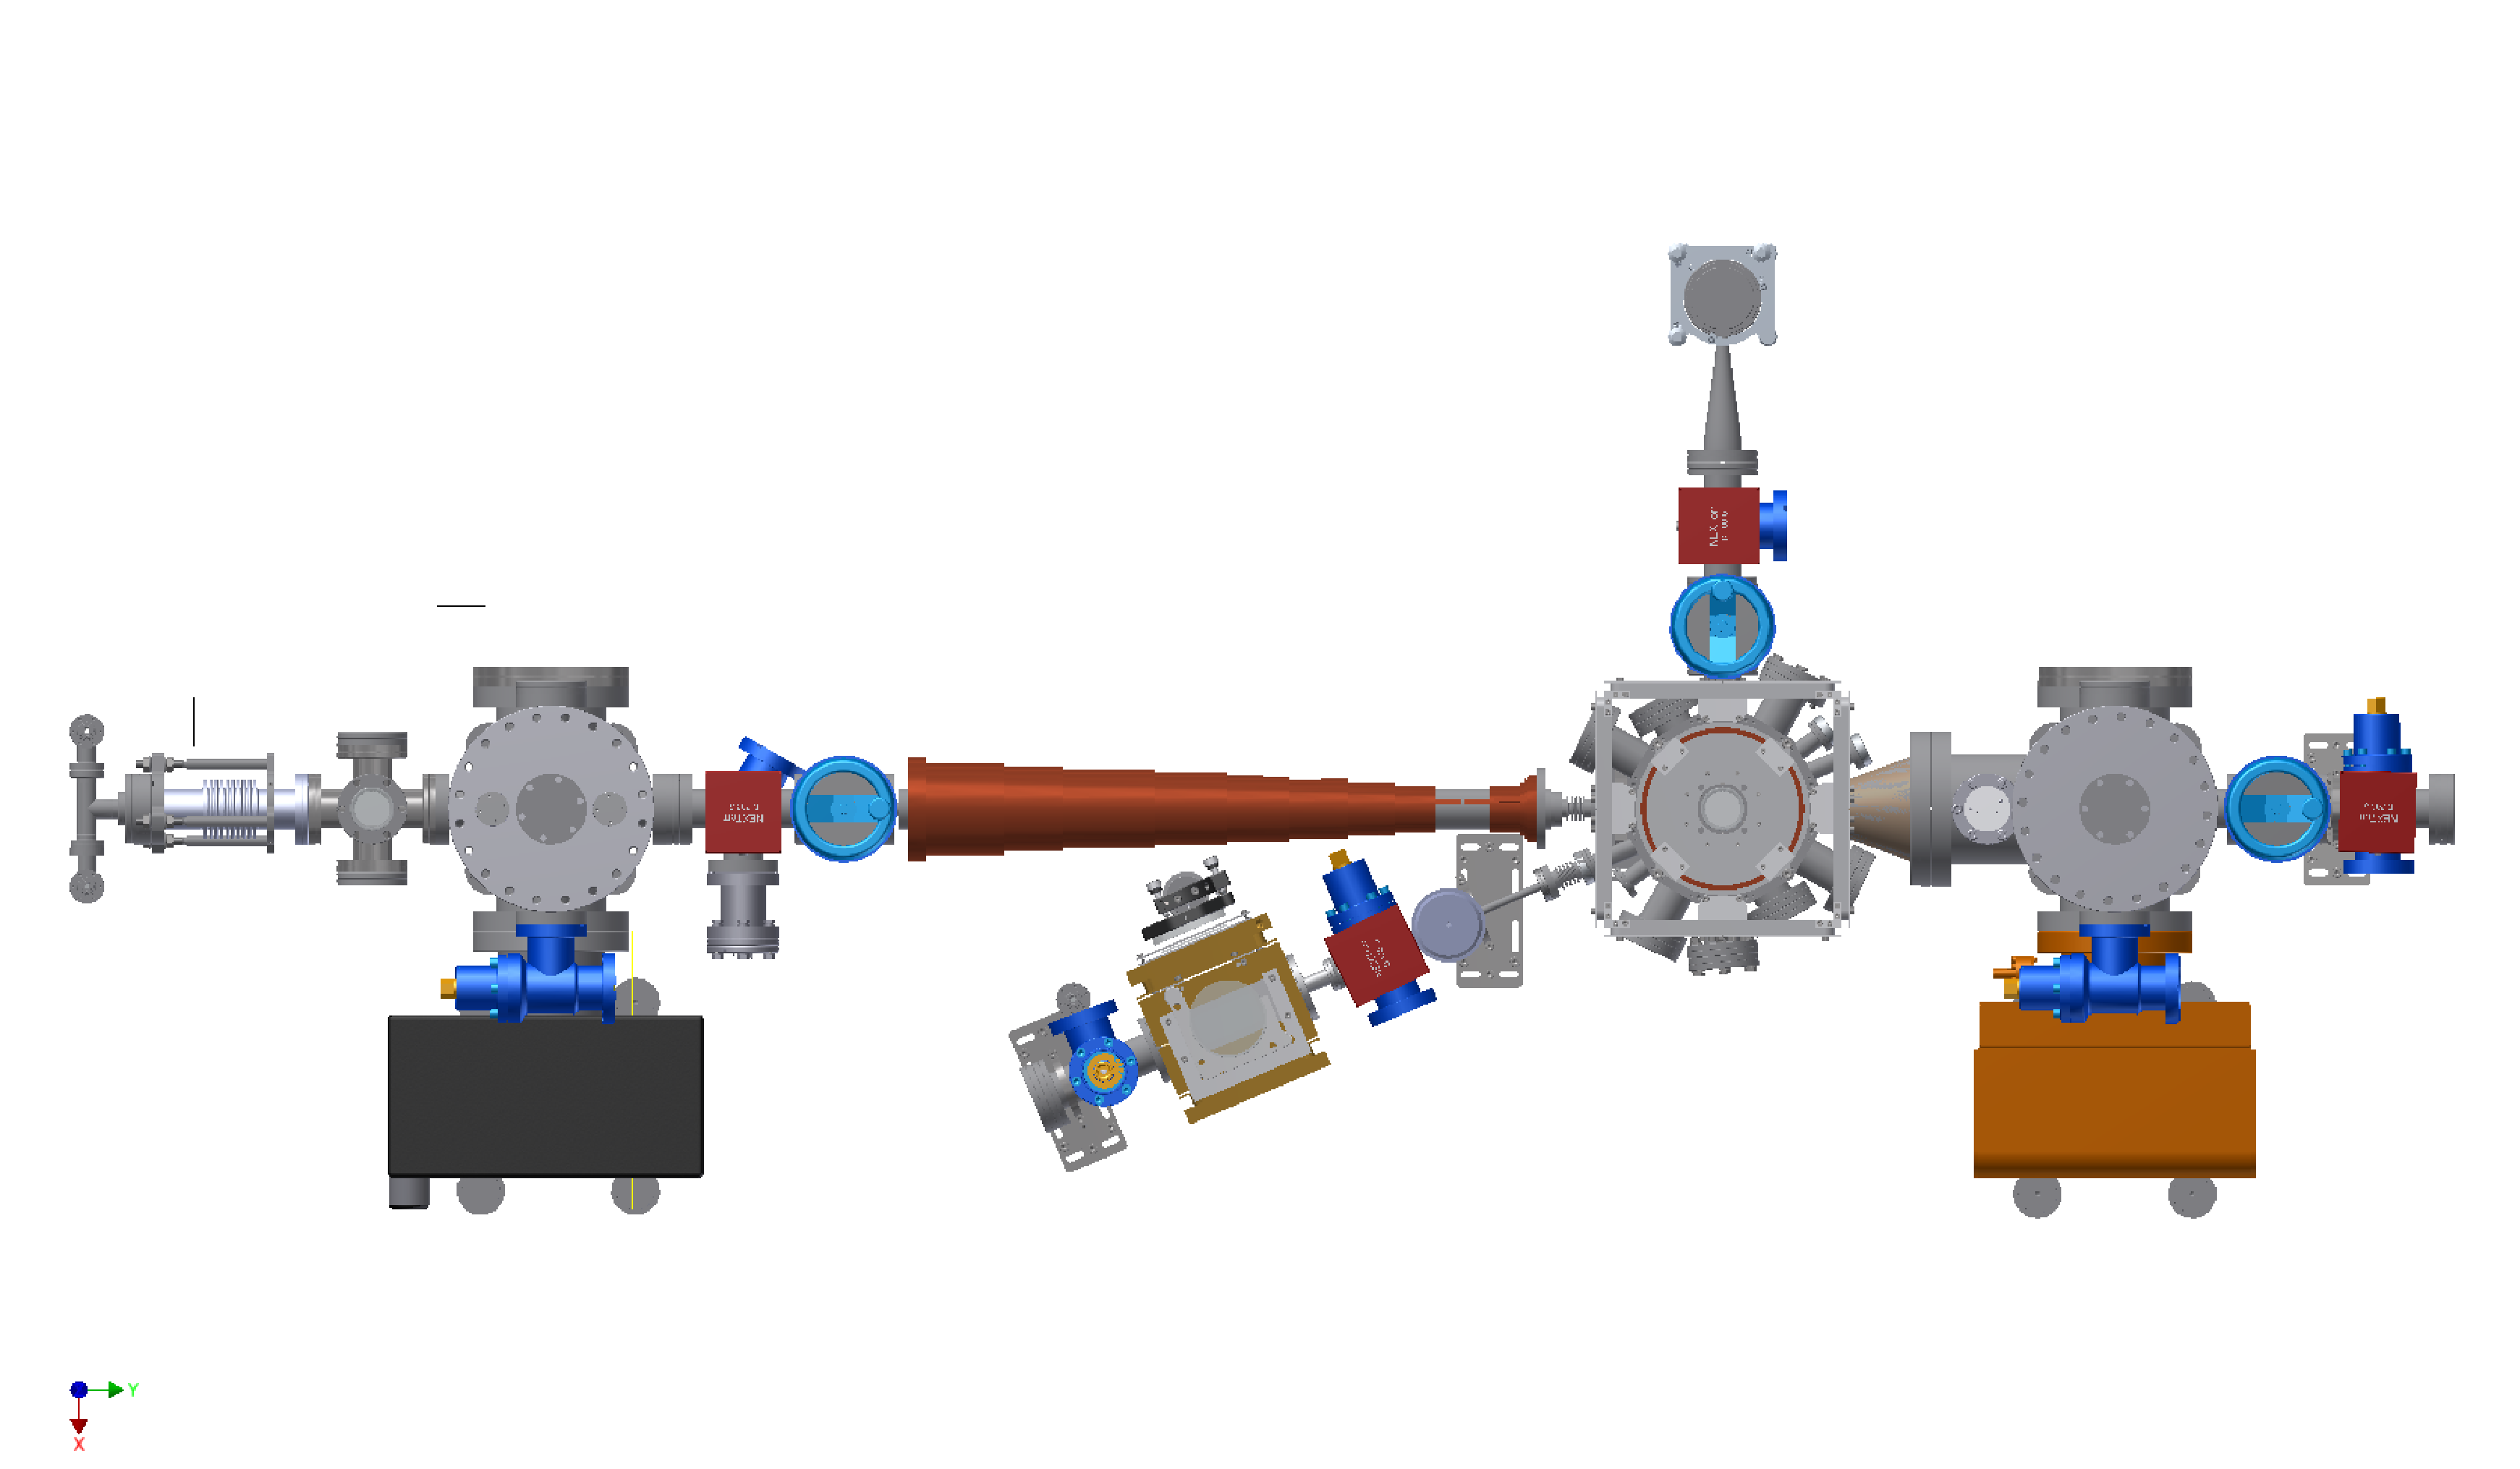
\includegraphics[width=\textwidth]{../media/image/apparatus.pdf}
  \caption{Apparatus of the cesium experiment. On the left-hand
    side an oven heats up the cesium source. A \gls{2d} \gls{mot} generates a
    particle beam twoards the pipe running through the Zeeman slower in the
    center. The Zeeman slower creates a magnetic field gradient, such that the
    atoms are in resonance with a cooling laser antiparallel to their flight
    direction. In the \gls{3d} \gls{mot} atoms are cooled even further until
    they are transported to a glass cell where they are loaded into the
    optical lattice and the actual experiments are conducted. Thank you to
    Till Klostermann and Hendrik v. Raven for providing the cesium apparatus
    render.}\label{fig:ultracold_atoms_setup}
\end{figure}
The apparatus used for ultracold-atom experiments comprises a vacuum system
with multiple chambers and windows for optical control and manipulation.
\Cref{fig:ultracold_atoms_setup} depicts an exemplary apparatus used
for such an experiment with cesium atoms. The oven on the left-hand side heats
up a cesium source to produce a hos gas of cesium atoms, which will then
diffuse to the right. Two orthogonal pairwise windows enable for transverse
cooling of the atoms in a \gls{2d} \gls{mot}. The Zeeman slower in the center
of the apparatus creates a magnetic field gradient such that the atoms are
always in resonance with a cooling laser antiparallel to the momentum
direction. Through this cooling step many of the atoms can be slowed down in
order to be captured in the \gls{3d} \gls{mot} where the atoms are cooled
further~\cite{Phillips1998}. Finally the atom cloud is transported to a glass
cell at the top, where they are loaded into an optical lattice. The glass
cell is placed between two high numerical aperture objectives for in-situ,
single site imaging and addressing.

One major ingredient to control and manipulate the ultracold atom ensemble in
the experimental chamber is the optical lattice itself. In
\Cref{fig:optical_lattice} a square \gls{2d} optical lattice is illustrated.
\begin{figure}[htb]
  \centering
  \begin{adjustbox}{width=\textwidth}
    %% Creator: Matplotlib, PGF backend
%%
%% To include the figure in your LaTeX document, write
%%   \input{<filename>.pgf}
%%
%% Make sure the required packages are loaded in your preamble
%%   \usepackage{pgf}
%%
%% Figures using additional raster images can only be included by \input if
%% they are in the same directory as the main LaTeX file. For loading figures
%% from other directories you can use the `import` package
%%   \usepackage{import}
%% and then include the figures with
%%   \import{<path to file>}{<filename>.pgf}
%%
%% Matplotlib used the following preamble
%%   \usepackage{amsmath}\usepackage{siunitx}\usepackage{lmodern}
%%   \usepackage{fontspec}
%%
\begingroup%
\makeatletter%
\begin{pgfpicture}%
\pgfpathrectangle{\pgfpointorigin}{\pgfqpoint{8.000000in}{8.000000in}}%
\pgfusepath{use as bounding box, clip}%
\begin{pgfscope}%
\pgfsetbuttcap%
\pgfsetmiterjoin%
\pgfsetlinewidth{0.000000pt}%
\definecolor{currentstroke}{rgb}{1.000000,1.000000,1.000000}%
\pgfsetstrokecolor{currentstroke}%
\pgfsetdash{}{0pt}%
\pgfpathmoveto{\pgfqpoint{0.000000in}{0.000000in}}%
\pgfpathlineto{\pgfqpoint{8.000000in}{0.000000in}}%
\pgfpathlineto{\pgfqpoint{8.000000in}{8.000000in}}%
\pgfpathlineto{\pgfqpoint{0.000000in}{8.000000in}}%
\pgfpathclose%
\pgfusepath{}%
\end{pgfscope}%
\begin{pgfscope}%
\pgfsetbuttcap%
\pgfsetmiterjoin%
\definecolor{currentfill}{rgb}{1.000000,1.000000,1.000000}%
\pgfsetfillcolor{currentfill}%
\pgfsetlinewidth{0.000000pt}%
\definecolor{currentstroke}{rgb}{0.000000,0.000000,0.000000}%
\pgfsetstrokecolor{currentstroke}%
\pgfsetstrokeopacity{0.000000}%
\pgfsetdash{}{0pt}%
\pgfpathmoveto{\pgfqpoint{2.300000in}{2.157576in}}%
\pgfpathlineto{\pgfqpoint{7.200000in}{2.157576in}}%
\pgfpathlineto{\pgfqpoint{7.200000in}{7.200000in}}%
\pgfpathlineto{\pgfqpoint{2.300000in}{7.200000in}}%
\pgfpathclose%
\pgfusepath{fill}%
\end{pgfscope}%
\begin{pgfscope}%
\pgfpathrectangle{\pgfqpoint{2.300000in}{2.157576in}}{\pgfqpoint{4.900000in}{5.042424in}}%
\pgfusepath{clip}%
\pgfsetbuttcap%
\pgfsetroundjoin%
\definecolor{currentfill}{rgb}{0.121569,0.466667,0.705882}%
\pgfsetfillcolor{currentfill}%
\pgfsetlinewidth{1.003750pt}%
\definecolor{currentstroke}{rgb}{0.121569,0.466667,0.705882}%
\pgfsetstrokecolor{currentstroke}%
\pgfsetdash{}{0pt}%
\pgfpathmoveto{\pgfqpoint{6.086364in}{5.553926in}}%
\pgfpathcurveto{\pgfqpoint{6.097414in}{5.553926in}}{\pgfqpoint{6.108013in}{5.558316in}}{\pgfqpoint{6.115826in}{5.566130in}}%
\pgfpathcurveto{\pgfqpoint{6.123640in}{5.573943in}}{\pgfqpoint{6.128030in}{5.584542in}}{\pgfqpoint{6.128030in}{5.595592in}}%
\pgfpathcurveto{\pgfqpoint{6.128030in}{5.606642in}}{\pgfqpoint{6.123640in}{5.617241in}}{\pgfqpoint{6.115826in}{5.625055in}}%
\pgfpathcurveto{\pgfqpoint{6.108013in}{5.632869in}}{\pgfqpoint{6.097414in}{5.637259in}}{\pgfqpoint{6.086364in}{5.637259in}}%
\pgfpathcurveto{\pgfqpoint{6.075314in}{5.637259in}}{\pgfqpoint{6.064714in}{5.632869in}}{\pgfqpoint{6.056901in}{5.625055in}}%
\pgfpathcurveto{\pgfqpoint{6.049087in}{5.617241in}}{\pgfqpoint{6.044697in}{5.606642in}}{\pgfqpoint{6.044697in}{5.595592in}}%
\pgfpathcurveto{\pgfqpoint{6.044697in}{5.584542in}}{\pgfqpoint{6.049087in}{5.573943in}}{\pgfqpoint{6.056901in}{5.566130in}}%
\pgfpathcurveto{\pgfqpoint{6.064714in}{5.558316in}}{\pgfqpoint{6.075314in}{5.553926in}}{\pgfqpoint{6.086364in}{5.553926in}}%
\pgfpathclose%
\pgfusepath{stroke,fill}%
\end{pgfscope}%
\begin{pgfscope}%
\pgfpathrectangle{\pgfqpoint{2.300000in}{2.157576in}}{\pgfqpoint{4.900000in}{5.042424in}}%
\pgfusepath{clip}%
\pgfsetbuttcap%
\pgfsetroundjoin%
\definecolor{currentfill}{rgb}{0.121569,0.466667,0.705882}%
\pgfsetfillcolor{currentfill}%
\pgfsetlinewidth{1.003750pt}%
\definecolor{currentstroke}{rgb}{0.121569,0.466667,0.705882}%
\pgfsetstrokecolor{currentstroke}%
\pgfsetdash{}{0pt}%
\pgfpathmoveto{\pgfqpoint{3.859091in}{3.261915in}}%
\pgfpathcurveto{\pgfqpoint{3.870141in}{3.261915in}}{\pgfqpoint{3.880740in}{3.266305in}}{\pgfqpoint{3.888554in}{3.274118in}}%
\pgfpathcurveto{\pgfqpoint{3.896367in}{3.281932in}}{\pgfqpoint{3.900758in}{3.292531in}}{\pgfqpoint{3.900758in}{3.303581in}}%
\pgfpathcurveto{\pgfqpoint{3.900758in}{3.314631in}}{\pgfqpoint{3.896367in}{3.325230in}}{\pgfqpoint{3.888554in}{3.333044in}}%
\pgfpathcurveto{\pgfqpoint{3.880740in}{3.340858in}}{\pgfqpoint{3.870141in}{3.345248in}}{\pgfqpoint{3.859091in}{3.345248in}}%
\pgfpathcurveto{\pgfqpoint{3.848041in}{3.345248in}}{\pgfqpoint{3.837442in}{3.340858in}}{\pgfqpoint{3.829628in}{3.333044in}}%
\pgfpathcurveto{\pgfqpoint{3.821815in}{3.325230in}}{\pgfqpoint{3.817424in}{3.314631in}}{\pgfqpoint{3.817424in}{3.303581in}}%
\pgfpathcurveto{\pgfqpoint{3.817424in}{3.292531in}}{\pgfqpoint{3.821815in}{3.281932in}}{\pgfqpoint{3.829628in}{3.274118in}}%
\pgfpathcurveto{\pgfqpoint{3.837442in}{3.266305in}}{\pgfqpoint{3.848041in}{3.261915in}}{\pgfqpoint{3.859091in}{3.261915in}}%
\pgfpathclose%
\pgfusepath{stroke,fill}%
\end{pgfscope}%
\begin{pgfscope}%
\pgfpathrectangle{\pgfqpoint{2.300000in}{2.157576in}}{\pgfqpoint{4.900000in}{5.042424in}}%
\pgfusepath{clip}%
\pgfsetbuttcap%
\pgfsetroundjoin%
\definecolor{currentfill}{rgb}{0.121569,0.466667,0.705882}%
\pgfsetfillcolor{currentfill}%
\pgfsetlinewidth{1.003750pt}%
\definecolor{currentstroke}{rgb}{0.121569,0.466667,0.705882}%
\pgfsetstrokecolor{currentstroke}%
\pgfsetdash{}{0pt}%
\pgfpathmoveto{\pgfqpoint{3.413636in}{6.470730in}}%
\pgfpathcurveto{\pgfqpoint{3.424686in}{6.470730in}}{\pgfqpoint{3.435286in}{6.475120in}}{\pgfqpoint{3.443099in}{6.482934in}}%
\pgfpathcurveto{\pgfqpoint{3.450913in}{6.490748in}}{\pgfqpoint{3.455303in}{6.501347in}}{\pgfqpoint{3.455303in}{6.512397in}}%
\pgfpathcurveto{\pgfqpoint{3.455303in}{6.523447in}}{\pgfqpoint{3.450913in}{6.534046in}}{\pgfqpoint{3.443099in}{6.541859in}}%
\pgfpathcurveto{\pgfqpoint{3.435286in}{6.549673in}}{\pgfqpoint{3.424686in}{6.554063in}}{\pgfqpoint{3.413636in}{6.554063in}}%
\pgfpathcurveto{\pgfqpoint{3.402586in}{6.554063in}}{\pgfqpoint{3.391987in}{6.549673in}}{\pgfqpoint{3.384174in}{6.541859in}}%
\pgfpathcurveto{\pgfqpoint{3.376360in}{6.534046in}}{\pgfqpoint{3.371970in}{6.523447in}}{\pgfqpoint{3.371970in}{6.512397in}}%
\pgfpathcurveto{\pgfqpoint{3.371970in}{6.501347in}}{\pgfqpoint{3.376360in}{6.490748in}}{\pgfqpoint{3.384174in}{6.482934in}}%
\pgfpathcurveto{\pgfqpoint{3.391987in}{6.475120in}}{\pgfqpoint{3.402586in}{6.470730in}}{\pgfqpoint{3.413636in}{6.470730in}}%
\pgfpathclose%
\pgfusepath{stroke,fill}%
\end{pgfscope}%
\begin{pgfscope}%
\pgfpathrectangle{\pgfqpoint{2.300000in}{2.157576in}}{\pgfqpoint{4.900000in}{5.042424in}}%
\pgfusepath{clip}%
\pgfsetbuttcap%
\pgfsetroundjoin%
\definecolor{currentfill}{rgb}{0.121569,0.466667,0.705882}%
\pgfsetfillcolor{currentfill}%
\pgfsetlinewidth{1.003750pt}%
\definecolor{currentstroke}{rgb}{0.121569,0.466667,0.705882}%
\pgfsetstrokecolor{currentstroke}%
\pgfsetdash{}{0pt}%
\pgfpathmoveto{\pgfqpoint{5.195455in}{5.553926in}}%
\pgfpathcurveto{\pgfqpoint{5.206505in}{5.553926in}}{\pgfqpoint{5.217104in}{5.558316in}}{\pgfqpoint{5.224917in}{5.566130in}}%
\pgfpathcurveto{\pgfqpoint{5.232731in}{5.573943in}}{\pgfqpoint{5.237121in}{5.584542in}}{\pgfqpoint{5.237121in}{5.595592in}}%
\pgfpathcurveto{\pgfqpoint{5.237121in}{5.606642in}}{\pgfqpoint{5.232731in}{5.617241in}}{\pgfqpoint{5.224917in}{5.625055in}}%
\pgfpathcurveto{\pgfqpoint{5.217104in}{5.632869in}}{\pgfqpoint{5.206505in}{5.637259in}}{\pgfqpoint{5.195455in}{5.637259in}}%
\pgfpathcurveto{\pgfqpoint{5.184404in}{5.637259in}}{\pgfqpoint{5.173805in}{5.632869in}}{\pgfqpoint{5.165992in}{5.625055in}}%
\pgfpathcurveto{\pgfqpoint{5.158178in}{5.617241in}}{\pgfqpoint{5.153788in}{5.606642in}}{\pgfqpoint{5.153788in}{5.595592in}}%
\pgfpathcurveto{\pgfqpoint{5.153788in}{5.584542in}}{\pgfqpoint{5.158178in}{5.573943in}}{\pgfqpoint{5.165992in}{5.566130in}}%
\pgfpathcurveto{\pgfqpoint{5.173805in}{5.558316in}}{\pgfqpoint{5.184404in}{5.553926in}}{\pgfqpoint{5.195455in}{5.553926in}}%
\pgfpathclose%
\pgfusepath{stroke,fill}%
\end{pgfscope}%
\begin{pgfscope}%
\pgfpathrectangle{\pgfqpoint{2.300000in}{2.157576in}}{\pgfqpoint{4.900000in}{5.042424in}}%
\pgfusepath{clip}%
\pgfsetbuttcap%
\pgfsetroundjoin%
\definecolor{currentfill}{rgb}{0.121569,0.466667,0.705882}%
\pgfsetfillcolor{currentfill}%
\pgfsetlinewidth{1.003750pt}%
\definecolor{currentstroke}{rgb}{0.121569,0.466667,0.705882}%
\pgfsetstrokecolor{currentstroke}%
\pgfsetdash{}{0pt}%
\pgfpathmoveto{\pgfqpoint{4.750000in}{6.470730in}}%
\pgfpathcurveto{\pgfqpoint{4.761050in}{6.470730in}}{\pgfqpoint{4.771649in}{6.475120in}}{\pgfqpoint{4.779463in}{6.482934in}}%
\pgfpathcurveto{\pgfqpoint{4.787276in}{6.490748in}}{\pgfqpoint{4.791667in}{6.501347in}}{\pgfqpoint{4.791667in}{6.512397in}}%
\pgfpathcurveto{\pgfqpoint{4.791667in}{6.523447in}}{\pgfqpoint{4.787276in}{6.534046in}}{\pgfqpoint{4.779463in}{6.541859in}}%
\pgfpathcurveto{\pgfqpoint{4.771649in}{6.549673in}}{\pgfqpoint{4.761050in}{6.554063in}}{\pgfqpoint{4.750000in}{6.554063in}}%
\pgfpathcurveto{\pgfqpoint{4.738950in}{6.554063in}}{\pgfqpoint{4.728351in}{6.549673in}}{\pgfqpoint{4.720537in}{6.541859in}}%
\pgfpathcurveto{\pgfqpoint{4.712724in}{6.534046in}}{\pgfqpoint{4.708333in}{6.523447in}}{\pgfqpoint{4.708333in}{6.512397in}}%
\pgfpathcurveto{\pgfqpoint{4.708333in}{6.501347in}}{\pgfqpoint{4.712724in}{6.490748in}}{\pgfqpoint{4.720537in}{6.482934in}}%
\pgfpathcurveto{\pgfqpoint{4.728351in}{6.475120in}}{\pgfqpoint{4.738950in}{6.470730in}}{\pgfqpoint{4.750000in}{6.470730in}}%
\pgfpathclose%
\pgfusepath{stroke,fill}%
\end{pgfscope}%
\begin{pgfscope}%
\pgfpathrectangle{\pgfqpoint{2.300000in}{2.157576in}}{\pgfqpoint{4.900000in}{5.042424in}}%
\pgfusepath{clip}%
\pgfsetbuttcap%
\pgfsetroundjoin%
\definecolor{currentfill}{rgb}{0.121569,0.466667,0.705882}%
\pgfsetfillcolor{currentfill}%
\pgfsetlinewidth{1.003750pt}%
\definecolor{currentstroke}{rgb}{0.121569,0.466667,0.705882}%
\pgfsetstrokecolor{currentstroke}%
\pgfsetdash{}{0pt}%
\pgfpathmoveto{\pgfqpoint{3.859091in}{6.470730in}}%
\pgfpathcurveto{\pgfqpoint{3.870141in}{6.470730in}}{\pgfqpoint{3.880740in}{6.475120in}}{\pgfqpoint{3.888554in}{6.482934in}}%
\pgfpathcurveto{\pgfqpoint{3.896367in}{6.490748in}}{\pgfqpoint{3.900758in}{6.501347in}}{\pgfqpoint{3.900758in}{6.512397in}}%
\pgfpathcurveto{\pgfqpoint{3.900758in}{6.523447in}}{\pgfqpoint{3.896367in}{6.534046in}}{\pgfqpoint{3.888554in}{6.541859in}}%
\pgfpathcurveto{\pgfqpoint{3.880740in}{6.549673in}}{\pgfqpoint{3.870141in}{6.554063in}}{\pgfqpoint{3.859091in}{6.554063in}}%
\pgfpathcurveto{\pgfqpoint{3.848041in}{6.554063in}}{\pgfqpoint{3.837442in}{6.549673in}}{\pgfqpoint{3.829628in}{6.541859in}}%
\pgfpathcurveto{\pgfqpoint{3.821815in}{6.534046in}}{\pgfqpoint{3.817424in}{6.523447in}}{\pgfqpoint{3.817424in}{6.512397in}}%
\pgfpathcurveto{\pgfqpoint{3.817424in}{6.501347in}}{\pgfqpoint{3.821815in}{6.490748in}}{\pgfqpoint{3.829628in}{6.482934in}}%
\pgfpathcurveto{\pgfqpoint{3.837442in}{6.475120in}}{\pgfqpoint{3.848041in}{6.470730in}}{\pgfqpoint{3.859091in}{6.470730in}}%
\pgfpathclose%
\pgfusepath{stroke,fill}%
\end{pgfscope}%
\begin{pgfscope}%
\pgfpathrectangle{\pgfqpoint{2.300000in}{2.157576in}}{\pgfqpoint{4.900000in}{5.042424in}}%
\pgfusepath{clip}%
\pgfsetbuttcap%
\pgfsetroundjoin%
\definecolor{currentfill}{rgb}{0.121569,0.466667,0.705882}%
\pgfsetfillcolor{currentfill}%
\pgfsetlinewidth{1.003750pt}%
\definecolor{currentstroke}{rgb}{0.121569,0.466667,0.705882}%
\pgfsetstrokecolor{currentstroke}%
\pgfsetdash{}{0pt}%
\pgfpathmoveto{\pgfqpoint{4.304545in}{3.261915in}}%
\pgfpathcurveto{\pgfqpoint{4.315596in}{3.261915in}}{\pgfqpoint{4.326195in}{3.266305in}}{\pgfqpoint{4.334008in}{3.274118in}}%
\pgfpathcurveto{\pgfqpoint{4.341822in}{3.281932in}}{\pgfqpoint{4.346212in}{3.292531in}}{\pgfqpoint{4.346212in}{3.303581in}}%
\pgfpathcurveto{\pgfqpoint{4.346212in}{3.314631in}}{\pgfqpoint{4.341822in}{3.325230in}}{\pgfqpoint{4.334008in}{3.333044in}}%
\pgfpathcurveto{\pgfqpoint{4.326195in}{3.340858in}}{\pgfqpoint{4.315596in}{3.345248in}}{\pgfqpoint{4.304545in}{3.345248in}}%
\pgfpathcurveto{\pgfqpoint{4.293495in}{3.345248in}}{\pgfqpoint{4.282896in}{3.340858in}}{\pgfqpoint{4.275083in}{3.333044in}}%
\pgfpathcurveto{\pgfqpoint{4.267269in}{3.325230in}}{\pgfqpoint{4.262879in}{3.314631in}}{\pgfqpoint{4.262879in}{3.303581in}}%
\pgfpathcurveto{\pgfqpoint{4.262879in}{3.292531in}}{\pgfqpoint{4.267269in}{3.281932in}}{\pgfqpoint{4.275083in}{3.274118in}}%
\pgfpathcurveto{\pgfqpoint{4.282896in}{3.266305in}}{\pgfqpoint{4.293495in}{3.261915in}}{\pgfqpoint{4.304545in}{3.261915in}}%
\pgfpathclose%
\pgfusepath{stroke,fill}%
\end{pgfscope}%
\begin{pgfscope}%
\pgfpathrectangle{\pgfqpoint{2.300000in}{2.157576in}}{\pgfqpoint{4.900000in}{5.042424in}}%
\pgfusepath{clip}%
\pgfsetbuttcap%
\pgfsetroundjoin%
\definecolor{currentfill}{rgb}{0.121569,0.466667,0.705882}%
\pgfsetfillcolor{currentfill}%
\pgfsetlinewidth{1.003750pt}%
\definecolor{currentstroke}{rgb}{0.121569,0.466667,0.705882}%
\pgfsetstrokecolor{currentstroke}%
\pgfsetdash{}{0pt}%
\pgfpathmoveto{\pgfqpoint{3.413636in}{6.012328in}}%
\pgfpathcurveto{\pgfqpoint{3.424686in}{6.012328in}}{\pgfqpoint{3.435286in}{6.016718in}}{\pgfqpoint{3.443099in}{6.024532in}}%
\pgfpathcurveto{\pgfqpoint{3.450913in}{6.032345in}}{\pgfqpoint{3.455303in}{6.042944in}}{\pgfqpoint{3.455303in}{6.053994in}}%
\pgfpathcurveto{\pgfqpoint{3.455303in}{6.065045in}}{\pgfqpoint{3.450913in}{6.075644in}}{\pgfqpoint{3.443099in}{6.083457in}}%
\pgfpathcurveto{\pgfqpoint{3.435286in}{6.091271in}}{\pgfqpoint{3.424686in}{6.095661in}}{\pgfqpoint{3.413636in}{6.095661in}}%
\pgfpathcurveto{\pgfqpoint{3.402586in}{6.095661in}}{\pgfqpoint{3.391987in}{6.091271in}}{\pgfqpoint{3.384174in}{6.083457in}}%
\pgfpathcurveto{\pgfqpoint{3.376360in}{6.075644in}}{\pgfqpoint{3.371970in}{6.065045in}}{\pgfqpoint{3.371970in}{6.053994in}}%
\pgfpathcurveto{\pgfqpoint{3.371970in}{6.042944in}}{\pgfqpoint{3.376360in}{6.032345in}}{\pgfqpoint{3.384174in}{6.024532in}}%
\pgfpathcurveto{\pgfqpoint{3.391987in}{6.016718in}}{\pgfqpoint{3.402586in}{6.012328in}}{\pgfqpoint{3.413636in}{6.012328in}}%
\pgfpathclose%
\pgfusepath{stroke,fill}%
\end{pgfscope}%
\begin{pgfscope}%
\pgfpathrectangle{\pgfqpoint{2.300000in}{2.157576in}}{\pgfqpoint{4.900000in}{5.042424in}}%
\pgfusepath{clip}%
\pgfsetbuttcap%
\pgfsetroundjoin%
\definecolor{currentfill}{rgb}{0.121569,0.466667,0.705882}%
\pgfsetfillcolor{currentfill}%
\pgfsetlinewidth{1.003750pt}%
\definecolor{currentstroke}{rgb}{0.121569,0.466667,0.705882}%
\pgfsetstrokecolor{currentstroke}%
\pgfsetdash{}{0pt}%
\pgfpathmoveto{\pgfqpoint{4.304545in}{3.720317in}}%
\pgfpathcurveto{\pgfqpoint{4.315596in}{3.720317in}}{\pgfqpoint{4.326195in}{3.724707in}}{\pgfqpoint{4.334008in}{3.732521in}}%
\pgfpathcurveto{\pgfqpoint{4.341822in}{3.740334in}}{\pgfqpoint{4.346212in}{3.750933in}}{\pgfqpoint{4.346212in}{3.761983in}}%
\pgfpathcurveto{\pgfqpoint{4.346212in}{3.773034in}}{\pgfqpoint{4.341822in}{3.783633in}}{\pgfqpoint{4.334008in}{3.791446in}}%
\pgfpathcurveto{\pgfqpoint{4.326195in}{3.799260in}}{\pgfqpoint{4.315596in}{3.803650in}}{\pgfqpoint{4.304545in}{3.803650in}}%
\pgfpathcurveto{\pgfqpoint{4.293495in}{3.803650in}}{\pgfqpoint{4.282896in}{3.799260in}}{\pgfqpoint{4.275083in}{3.791446in}}%
\pgfpathcurveto{\pgfqpoint{4.267269in}{3.783633in}}{\pgfqpoint{4.262879in}{3.773034in}}{\pgfqpoint{4.262879in}{3.761983in}}%
\pgfpathcurveto{\pgfqpoint{4.262879in}{3.750933in}}{\pgfqpoint{4.267269in}{3.740334in}}{\pgfqpoint{4.275083in}{3.732521in}}%
\pgfpathcurveto{\pgfqpoint{4.282896in}{3.724707in}}{\pgfqpoint{4.293495in}{3.720317in}}{\pgfqpoint{4.304545in}{3.720317in}}%
\pgfpathclose%
\pgfusepath{stroke,fill}%
\end{pgfscope}%
\begin{pgfscope}%
\pgfpathrectangle{\pgfqpoint{2.300000in}{2.157576in}}{\pgfqpoint{4.900000in}{5.042424in}}%
\pgfusepath{clip}%
\pgfsetbuttcap%
\pgfsetroundjoin%
\definecolor{currentfill}{rgb}{0.121569,0.466667,0.705882}%
\pgfsetfillcolor{currentfill}%
\pgfsetlinewidth{1.003750pt}%
\definecolor{currentstroke}{rgb}{0.121569,0.466667,0.705882}%
\pgfsetstrokecolor{currentstroke}%
\pgfsetdash{}{0pt}%
\pgfpathmoveto{\pgfqpoint{3.413636in}{3.261915in}}%
\pgfpathcurveto{\pgfqpoint{3.424686in}{3.261915in}}{\pgfqpoint{3.435286in}{3.266305in}}{\pgfqpoint{3.443099in}{3.274118in}}%
\pgfpathcurveto{\pgfqpoint{3.450913in}{3.281932in}}{\pgfqpoint{3.455303in}{3.292531in}}{\pgfqpoint{3.455303in}{3.303581in}}%
\pgfpathcurveto{\pgfqpoint{3.455303in}{3.314631in}}{\pgfqpoint{3.450913in}{3.325230in}}{\pgfqpoint{3.443099in}{3.333044in}}%
\pgfpathcurveto{\pgfqpoint{3.435286in}{3.340858in}}{\pgfqpoint{3.424686in}{3.345248in}}{\pgfqpoint{3.413636in}{3.345248in}}%
\pgfpathcurveto{\pgfqpoint{3.402586in}{3.345248in}}{\pgfqpoint{3.391987in}{3.340858in}}{\pgfqpoint{3.384174in}{3.333044in}}%
\pgfpathcurveto{\pgfqpoint{3.376360in}{3.325230in}}{\pgfqpoint{3.371970in}{3.314631in}}{\pgfqpoint{3.371970in}{3.303581in}}%
\pgfpathcurveto{\pgfqpoint{3.371970in}{3.292531in}}{\pgfqpoint{3.376360in}{3.281932in}}{\pgfqpoint{3.384174in}{3.274118in}}%
\pgfpathcurveto{\pgfqpoint{3.391987in}{3.266305in}}{\pgfqpoint{3.402586in}{3.261915in}}{\pgfqpoint{3.413636in}{3.261915in}}%
\pgfpathclose%
\pgfusepath{stroke,fill}%
\end{pgfscope}%
\begin{pgfscope}%
\pgfpathrectangle{\pgfqpoint{2.300000in}{2.157576in}}{\pgfqpoint{4.900000in}{5.042424in}}%
\pgfusepath{clip}%
\pgfsetbuttcap%
\pgfsetroundjoin%
\definecolor{currentfill}{rgb}{0.121569,0.466667,0.705882}%
\pgfsetfillcolor{currentfill}%
\pgfsetlinewidth{1.003750pt}%
\definecolor{currentstroke}{rgb}{0.121569,0.466667,0.705882}%
\pgfsetstrokecolor{currentstroke}%
\pgfsetdash{}{0pt}%
\pgfpathmoveto{\pgfqpoint{3.859091in}{5.553926in}}%
\pgfpathcurveto{\pgfqpoint{3.870141in}{5.553926in}}{\pgfqpoint{3.880740in}{5.558316in}}{\pgfqpoint{3.888554in}{5.566130in}}%
\pgfpathcurveto{\pgfqpoint{3.896367in}{5.573943in}}{\pgfqpoint{3.900758in}{5.584542in}}{\pgfqpoint{3.900758in}{5.595592in}}%
\pgfpathcurveto{\pgfqpoint{3.900758in}{5.606642in}}{\pgfqpoint{3.896367in}{5.617241in}}{\pgfqpoint{3.888554in}{5.625055in}}%
\pgfpathcurveto{\pgfqpoint{3.880740in}{5.632869in}}{\pgfqpoint{3.870141in}{5.637259in}}{\pgfqpoint{3.859091in}{5.637259in}}%
\pgfpathcurveto{\pgfqpoint{3.848041in}{5.637259in}}{\pgfqpoint{3.837442in}{5.632869in}}{\pgfqpoint{3.829628in}{5.625055in}}%
\pgfpathcurveto{\pgfqpoint{3.821815in}{5.617241in}}{\pgfqpoint{3.817424in}{5.606642in}}{\pgfqpoint{3.817424in}{5.595592in}}%
\pgfpathcurveto{\pgfqpoint{3.817424in}{5.584542in}}{\pgfqpoint{3.821815in}{5.573943in}}{\pgfqpoint{3.829628in}{5.566130in}}%
\pgfpathcurveto{\pgfqpoint{3.837442in}{5.558316in}}{\pgfqpoint{3.848041in}{5.553926in}}{\pgfqpoint{3.859091in}{5.553926in}}%
\pgfpathclose%
\pgfusepath{stroke,fill}%
\end{pgfscope}%
\begin{pgfscope}%
\pgfpathrectangle{\pgfqpoint{2.300000in}{2.157576in}}{\pgfqpoint{4.900000in}{5.042424in}}%
\pgfusepath{clip}%
\pgfsetbuttcap%
\pgfsetroundjoin%
\definecolor{currentfill}{rgb}{0.121569,0.466667,0.705882}%
\pgfsetfillcolor{currentfill}%
\pgfsetlinewidth{1.003750pt}%
\definecolor{currentstroke}{rgb}{0.121569,0.466667,0.705882}%
\pgfsetstrokecolor{currentstroke}%
\pgfsetdash{}{0pt}%
\pgfpathmoveto{\pgfqpoint{3.859091in}{4.178719in}}%
\pgfpathcurveto{\pgfqpoint{3.870141in}{4.178719in}}{\pgfqpoint{3.880740in}{4.183109in}}{\pgfqpoint{3.888554in}{4.190923in}}%
\pgfpathcurveto{\pgfqpoint{3.896367in}{4.198737in}}{\pgfqpoint{3.900758in}{4.209336in}}{\pgfqpoint{3.900758in}{4.220386in}}%
\pgfpathcurveto{\pgfqpoint{3.900758in}{4.231436in}}{\pgfqpoint{3.896367in}{4.242035in}}{\pgfqpoint{3.888554in}{4.249848in}}%
\pgfpathcurveto{\pgfqpoint{3.880740in}{4.257662in}}{\pgfqpoint{3.870141in}{4.262052in}}{\pgfqpoint{3.859091in}{4.262052in}}%
\pgfpathcurveto{\pgfqpoint{3.848041in}{4.262052in}}{\pgfqpoint{3.837442in}{4.257662in}}{\pgfqpoint{3.829628in}{4.249848in}}%
\pgfpathcurveto{\pgfqpoint{3.821815in}{4.242035in}}{\pgfqpoint{3.817424in}{4.231436in}}{\pgfqpoint{3.817424in}{4.220386in}}%
\pgfpathcurveto{\pgfqpoint{3.817424in}{4.209336in}}{\pgfqpoint{3.821815in}{4.198737in}}{\pgfqpoint{3.829628in}{4.190923in}}%
\pgfpathcurveto{\pgfqpoint{3.837442in}{4.183109in}}{\pgfqpoint{3.848041in}{4.178719in}}{\pgfqpoint{3.859091in}{4.178719in}}%
\pgfpathclose%
\pgfusepath{stroke,fill}%
\end{pgfscope}%
\begin{pgfscope}%
\pgfpathrectangle{\pgfqpoint{2.300000in}{2.157576in}}{\pgfqpoint{4.900000in}{5.042424in}}%
\pgfusepath{clip}%
\pgfsetbuttcap%
\pgfsetroundjoin%
\definecolor{currentfill}{rgb}{0.121569,0.466667,0.705882}%
\pgfsetfillcolor{currentfill}%
\pgfsetlinewidth{1.003750pt}%
\definecolor{currentstroke}{rgb}{0.121569,0.466667,0.705882}%
\pgfsetstrokecolor{currentstroke}%
\pgfsetdash{}{0pt}%
\pgfpathmoveto{\pgfqpoint{4.304545in}{4.637121in}}%
\pgfpathcurveto{\pgfqpoint{4.315596in}{4.637121in}}{\pgfqpoint{4.326195in}{4.641511in}}{\pgfqpoint{4.334008in}{4.649325in}}%
\pgfpathcurveto{\pgfqpoint{4.341822in}{4.657139in}}{\pgfqpoint{4.346212in}{4.667738in}}{\pgfqpoint{4.346212in}{4.678788in}}%
\pgfpathcurveto{\pgfqpoint{4.346212in}{4.689838in}}{\pgfqpoint{4.341822in}{4.700437in}}{\pgfqpoint{4.334008in}{4.708251in}}%
\pgfpathcurveto{\pgfqpoint{4.326195in}{4.716064in}}{\pgfqpoint{4.315596in}{4.720455in}}{\pgfqpoint{4.304545in}{4.720455in}}%
\pgfpathcurveto{\pgfqpoint{4.293495in}{4.720455in}}{\pgfqpoint{4.282896in}{4.716064in}}{\pgfqpoint{4.275083in}{4.708251in}}%
\pgfpathcurveto{\pgfqpoint{4.267269in}{4.700437in}}{\pgfqpoint{4.262879in}{4.689838in}}{\pgfqpoint{4.262879in}{4.678788in}}%
\pgfpathcurveto{\pgfqpoint{4.262879in}{4.667738in}}{\pgfqpoint{4.267269in}{4.657139in}}{\pgfqpoint{4.275083in}{4.649325in}}%
\pgfpathcurveto{\pgfqpoint{4.282896in}{4.641511in}}{\pgfqpoint{4.293495in}{4.637121in}}{\pgfqpoint{4.304545in}{4.637121in}}%
\pgfpathclose%
\pgfusepath{stroke,fill}%
\end{pgfscope}%
\begin{pgfscope}%
\pgfpathrectangle{\pgfqpoint{2.300000in}{2.157576in}}{\pgfqpoint{4.900000in}{5.042424in}}%
\pgfusepath{clip}%
\pgfsetbuttcap%
\pgfsetroundjoin%
\definecolor{currentfill}{rgb}{0.121569,0.466667,0.705882}%
\pgfsetfillcolor{currentfill}%
\pgfsetlinewidth{1.003750pt}%
\definecolor{currentstroke}{rgb}{0.121569,0.466667,0.705882}%
\pgfsetstrokecolor{currentstroke}%
\pgfsetdash{}{0pt}%
\pgfpathmoveto{\pgfqpoint{6.531818in}{3.720317in}}%
\pgfpathcurveto{\pgfqpoint{6.542868in}{3.720317in}}{\pgfqpoint{6.553467in}{3.724707in}}{\pgfqpoint{6.561281in}{3.732521in}}%
\pgfpathcurveto{\pgfqpoint{6.569095in}{3.740334in}}{\pgfqpoint{6.573485in}{3.750933in}}{\pgfqpoint{6.573485in}{3.761983in}}%
\pgfpathcurveto{\pgfqpoint{6.573485in}{3.773034in}}{\pgfqpoint{6.569095in}{3.783633in}}{\pgfqpoint{6.561281in}{3.791446in}}%
\pgfpathcurveto{\pgfqpoint{6.553467in}{3.799260in}}{\pgfqpoint{6.542868in}{3.803650in}}{\pgfqpoint{6.531818in}{3.803650in}}%
\pgfpathcurveto{\pgfqpoint{6.520768in}{3.803650in}}{\pgfqpoint{6.510169in}{3.799260in}}{\pgfqpoint{6.502355in}{3.791446in}}%
\pgfpathcurveto{\pgfqpoint{6.494542in}{3.783633in}}{\pgfqpoint{6.490152in}{3.773034in}}{\pgfqpoint{6.490152in}{3.761983in}}%
\pgfpathcurveto{\pgfqpoint{6.490152in}{3.750933in}}{\pgfqpoint{6.494542in}{3.740334in}}{\pgfqpoint{6.502355in}{3.732521in}}%
\pgfpathcurveto{\pgfqpoint{6.510169in}{3.724707in}}{\pgfqpoint{6.520768in}{3.720317in}}{\pgfqpoint{6.531818in}{3.720317in}}%
\pgfpathclose%
\pgfusepath{stroke,fill}%
\end{pgfscope}%
\begin{pgfscope}%
\pgfpathrectangle{\pgfqpoint{2.300000in}{2.157576in}}{\pgfqpoint{4.900000in}{5.042424in}}%
\pgfusepath{clip}%
\pgfsetbuttcap%
\pgfsetroundjoin%
\definecolor{currentfill}{rgb}{0.121569,0.466667,0.705882}%
\pgfsetfillcolor{currentfill}%
\pgfsetlinewidth{1.003750pt}%
\definecolor{currentstroke}{rgb}{0.121569,0.466667,0.705882}%
\pgfsetstrokecolor{currentstroke}%
\pgfsetdash{}{0pt}%
\pgfpathmoveto{\pgfqpoint{5.195455in}{4.637121in}}%
\pgfpathcurveto{\pgfqpoint{5.206505in}{4.637121in}}{\pgfqpoint{5.217104in}{4.641511in}}{\pgfqpoint{5.224917in}{4.649325in}}%
\pgfpathcurveto{\pgfqpoint{5.232731in}{4.657139in}}{\pgfqpoint{5.237121in}{4.667738in}}{\pgfqpoint{5.237121in}{4.678788in}}%
\pgfpathcurveto{\pgfqpoint{5.237121in}{4.689838in}}{\pgfqpoint{5.232731in}{4.700437in}}{\pgfqpoint{5.224917in}{4.708251in}}%
\pgfpathcurveto{\pgfqpoint{5.217104in}{4.716064in}}{\pgfqpoint{5.206505in}{4.720455in}}{\pgfqpoint{5.195455in}{4.720455in}}%
\pgfpathcurveto{\pgfqpoint{5.184404in}{4.720455in}}{\pgfqpoint{5.173805in}{4.716064in}}{\pgfqpoint{5.165992in}{4.708251in}}%
\pgfpathcurveto{\pgfqpoint{5.158178in}{4.700437in}}{\pgfqpoint{5.153788in}{4.689838in}}{\pgfqpoint{5.153788in}{4.678788in}}%
\pgfpathcurveto{\pgfqpoint{5.153788in}{4.667738in}}{\pgfqpoint{5.158178in}{4.657139in}}{\pgfqpoint{5.165992in}{4.649325in}}%
\pgfpathcurveto{\pgfqpoint{5.173805in}{4.641511in}}{\pgfqpoint{5.184404in}{4.637121in}}{\pgfqpoint{5.195455in}{4.637121in}}%
\pgfpathclose%
\pgfusepath{stroke,fill}%
\end{pgfscope}%
\begin{pgfscope}%
\pgfpathrectangle{\pgfqpoint{2.300000in}{2.157576in}}{\pgfqpoint{4.900000in}{5.042424in}}%
\pgfusepath{clip}%
\pgfsetbuttcap%
\pgfsetroundjoin%
\definecolor{currentfill}{rgb}{0.121569,0.466667,0.705882}%
\pgfsetfillcolor{currentfill}%
\pgfsetlinewidth{1.003750pt}%
\definecolor{currentstroke}{rgb}{0.121569,0.466667,0.705882}%
\pgfsetstrokecolor{currentstroke}%
\pgfsetdash{}{0pt}%
\pgfpathmoveto{\pgfqpoint{5.195455in}{2.803512in}}%
\pgfpathcurveto{\pgfqpoint{5.206505in}{2.803512in}}{\pgfqpoint{5.217104in}{2.807903in}}{\pgfqpoint{5.224917in}{2.815716in}}%
\pgfpathcurveto{\pgfqpoint{5.232731in}{2.823530in}}{\pgfqpoint{5.237121in}{2.834129in}}{\pgfqpoint{5.237121in}{2.845179in}}%
\pgfpathcurveto{\pgfqpoint{5.237121in}{2.856229in}}{\pgfqpoint{5.232731in}{2.866828in}}{\pgfqpoint{5.224917in}{2.874642in}}%
\pgfpathcurveto{\pgfqpoint{5.217104in}{2.882455in}}{\pgfqpoint{5.206505in}{2.886846in}}{\pgfqpoint{5.195455in}{2.886846in}}%
\pgfpathcurveto{\pgfqpoint{5.184404in}{2.886846in}}{\pgfqpoint{5.173805in}{2.882455in}}{\pgfqpoint{5.165992in}{2.874642in}}%
\pgfpathcurveto{\pgfqpoint{5.158178in}{2.866828in}}{\pgfqpoint{5.153788in}{2.856229in}}{\pgfqpoint{5.153788in}{2.845179in}}%
\pgfpathcurveto{\pgfqpoint{5.153788in}{2.834129in}}{\pgfqpoint{5.158178in}{2.823530in}}{\pgfqpoint{5.165992in}{2.815716in}}%
\pgfpathcurveto{\pgfqpoint{5.173805in}{2.807903in}}{\pgfqpoint{5.184404in}{2.803512in}}{\pgfqpoint{5.195455in}{2.803512in}}%
\pgfpathclose%
\pgfusepath{stroke,fill}%
\end{pgfscope}%
\begin{pgfscope}%
\pgfpathrectangle{\pgfqpoint{2.300000in}{2.157576in}}{\pgfqpoint{4.900000in}{5.042424in}}%
\pgfusepath{clip}%
\pgfsetbuttcap%
\pgfsetroundjoin%
\definecolor{currentfill}{rgb}{0.121569,0.466667,0.705882}%
\pgfsetfillcolor{currentfill}%
\pgfsetlinewidth{1.003750pt}%
\definecolor{currentstroke}{rgb}{0.121569,0.466667,0.705882}%
\pgfsetstrokecolor{currentstroke}%
\pgfsetdash{}{0pt}%
\pgfpathmoveto{\pgfqpoint{5.195455in}{2.803512in}}%
\pgfpathcurveto{\pgfqpoint{5.206505in}{2.803512in}}{\pgfqpoint{5.217104in}{2.807903in}}{\pgfqpoint{5.224917in}{2.815716in}}%
\pgfpathcurveto{\pgfqpoint{5.232731in}{2.823530in}}{\pgfqpoint{5.237121in}{2.834129in}}{\pgfqpoint{5.237121in}{2.845179in}}%
\pgfpathcurveto{\pgfqpoint{5.237121in}{2.856229in}}{\pgfqpoint{5.232731in}{2.866828in}}{\pgfqpoint{5.224917in}{2.874642in}}%
\pgfpathcurveto{\pgfqpoint{5.217104in}{2.882455in}}{\pgfqpoint{5.206505in}{2.886846in}}{\pgfqpoint{5.195455in}{2.886846in}}%
\pgfpathcurveto{\pgfqpoint{5.184404in}{2.886846in}}{\pgfqpoint{5.173805in}{2.882455in}}{\pgfqpoint{5.165992in}{2.874642in}}%
\pgfpathcurveto{\pgfqpoint{5.158178in}{2.866828in}}{\pgfqpoint{5.153788in}{2.856229in}}{\pgfqpoint{5.153788in}{2.845179in}}%
\pgfpathcurveto{\pgfqpoint{5.153788in}{2.834129in}}{\pgfqpoint{5.158178in}{2.823530in}}{\pgfqpoint{5.165992in}{2.815716in}}%
\pgfpathcurveto{\pgfqpoint{5.173805in}{2.807903in}}{\pgfqpoint{5.184404in}{2.803512in}}{\pgfqpoint{5.195455in}{2.803512in}}%
\pgfpathclose%
\pgfusepath{stroke,fill}%
\end{pgfscope}%
\begin{pgfscope}%
\pgfpathrectangle{\pgfqpoint{2.300000in}{2.157576in}}{\pgfqpoint{4.900000in}{5.042424in}}%
\pgfusepath{clip}%
\pgfsetbuttcap%
\pgfsetroundjoin%
\definecolor{currentfill}{rgb}{0.121569,0.466667,0.705882}%
\pgfsetfillcolor{currentfill}%
\pgfsetlinewidth{1.003750pt}%
\definecolor{currentstroke}{rgb}{0.121569,0.466667,0.705882}%
\pgfsetstrokecolor{currentstroke}%
\pgfsetdash{}{0pt}%
\pgfpathmoveto{\pgfqpoint{4.750000in}{4.178719in}}%
\pgfpathcurveto{\pgfqpoint{4.761050in}{4.178719in}}{\pgfqpoint{4.771649in}{4.183109in}}{\pgfqpoint{4.779463in}{4.190923in}}%
\pgfpathcurveto{\pgfqpoint{4.787276in}{4.198737in}}{\pgfqpoint{4.791667in}{4.209336in}}{\pgfqpoint{4.791667in}{4.220386in}}%
\pgfpathcurveto{\pgfqpoint{4.791667in}{4.231436in}}{\pgfqpoint{4.787276in}{4.242035in}}{\pgfqpoint{4.779463in}{4.249848in}}%
\pgfpathcurveto{\pgfqpoint{4.771649in}{4.257662in}}{\pgfqpoint{4.761050in}{4.262052in}}{\pgfqpoint{4.750000in}{4.262052in}}%
\pgfpathcurveto{\pgfqpoint{4.738950in}{4.262052in}}{\pgfqpoint{4.728351in}{4.257662in}}{\pgfqpoint{4.720537in}{4.249848in}}%
\pgfpathcurveto{\pgfqpoint{4.712724in}{4.242035in}}{\pgfqpoint{4.708333in}{4.231436in}}{\pgfqpoint{4.708333in}{4.220386in}}%
\pgfpathcurveto{\pgfqpoint{4.708333in}{4.209336in}}{\pgfqpoint{4.712724in}{4.198737in}}{\pgfqpoint{4.720537in}{4.190923in}}%
\pgfpathcurveto{\pgfqpoint{4.728351in}{4.183109in}}{\pgfqpoint{4.738950in}{4.178719in}}{\pgfqpoint{4.750000in}{4.178719in}}%
\pgfpathclose%
\pgfusepath{stroke,fill}%
\end{pgfscope}%
\begin{pgfscope}%
\pgfpathrectangle{\pgfqpoint{2.300000in}{2.157576in}}{\pgfqpoint{4.900000in}{5.042424in}}%
\pgfusepath{clip}%
\pgfsetbuttcap%
\pgfsetroundjoin%
\definecolor{currentfill}{rgb}{0.121569,0.466667,0.705882}%
\pgfsetfillcolor{currentfill}%
\pgfsetlinewidth{1.003750pt}%
\definecolor{currentstroke}{rgb}{0.121569,0.466667,0.705882}%
\pgfsetstrokecolor{currentstroke}%
\pgfsetdash{}{0pt}%
\pgfpathmoveto{\pgfqpoint{6.531818in}{5.095523in}}%
\pgfpathcurveto{\pgfqpoint{6.542868in}{5.095523in}}{\pgfqpoint{6.553467in}{5.099914in}}{\pgfqpoint{6.561281in}{5.107727in}}%
\pgfpathcurveto{\pgfqpoint{6.569095in}{5.115541in}}{\pgfqpoint{6.573485in}{5.126140in}}{\pgfqpoint{6.573485in}{5.137190in}}%
\pgfpathcurveto{\pgfqpoint{6.573485in}{5.148240in}}{\pgfqpoint{6.569095in}{5.158839in}}{\pgfqpoint{6.561281in}{5.166653in}}%
\pgfpathcurveto{\pgfqpoint{6.553467in}{5.174466in}}{\pgfqpoint{6.542868in}{5.178857in}}{\pgfqpoint{6.531818in}{5.178857in}}%
\pgfpathcurveto{\pgfqpoint{6.520768in}{5.178857in}}{\pgfqpoint{6.510169in}{5.174466in}}{\pgfqpoint{6.502355in}{5.166653in}}%
\pgfpathcurveto{\pgfqpoint{6.494542in}{5.158839in}}{\pgfqpoint{6.490152in}{5.148240in}}{\pgfqpoint{6.490152in}{5.137190in}}%
\pgfpathcurveto{\pgfqpoint{6.490152in}{5.126140in}}{\pgfqpoint{6.494542in}{5.115541in}}{\pgfqpoint{6.502355in}{5.107727in}}%
\pgfpathcurveto{\pgfqpoint{6.510169in}{5.099914in}}{\pgfqpoint{6.520768in}{5.095523in}}{\pgfqpoint{6.531818in}{5.095523in}}%
\pgfpathclose%
\pgfusepath{stroke,fill}%
\end{pgfscope}%
\begin{pgfscope}%
\pgfpathrectangle{\pgfqpoint{2.300000in}{2.157576in}}{\pgfqpoint{4.900000in}{5.042424in}}%
\pgfusepath{clip}%
\pgfsetbuttcap%
\pgfsetroundjoin%
\definecolor{currentfill}{rgb}{0.121569,0.466667,0.705882}%
\pgfsetfillcolor{currentfill}%
\pgfsetlinewidth{1.003750pt}%
\definecolor{currentstroke}{rgb}{0.121569,0.466667,0.705882}%
\pgfsetstrokecolor{currentstroke}%
\pgfsetdash{}{0pt}%
\pgfpathmoveto{\pgfqpoint{3.413636in}{4.178719in}}%
\pgfpathcurveto{\pgfqpoint{3.424686in}{4.178719in}}{\pgfqpoint{3.435286in}{4.183109in}}{\pgfqpoint{3.443099in}{4.190923in}}%
\pgfpathcurveto{\pgfqpoint{3.450913in}{4.198737in}}{\pgfqpoint{3.455303in}{4.209336in}}{\pgfqpoint{3.455303in}{4.220386in}}%
\pgfpathcurveto{\pgfqpoint{3.455303in}{4.231436in}}{\pgfqpoint{3.450913in}{4.242035in}}{\pgfqpoint{3.443099in}{4.249848in}}%
\pgfpathcurveto{\pgfqpoint{3.435286in}{4.257662in}}{\pgfqpoint{3.424686in}{4.262052in}}{\pgfqpoint{3.413636in}{4.262052in}}%
\pgfpathcurveto{\pgfqpoint{3.402586in}{4.262052in}}{\pgfqpoint{3.391987in}{4.257662in}}{\pgfqpoint{3.384174in}{4.249848in}}%
\pgfpathcurveto{\pgfqpoint{3.376360in}{4.242035in}}{\pgfqpoint{3.371970in}{4.231436in}}{\pgfqpoint{3.371970in}{4.220386in}}%
\pgfpathcurveto{\pgfqpoint{3.371970in}{4.209336in}}{\pgfqpoint{3.376360in}{4.198737in}}{\pgfqpoint{3.384174in}{4.190923in}}%
\pgfpathcurveto{\pgfqpoint{3.391987in}{4.183109in}}{\pgfqpoint{3.402586in}{4.178719in}}{\pgfqpoint{3.413636in}{4.178719in}}%
\pgfpathclose%
\pgfusepath{stroke,fill}%
\end{pgfscope}%
\begin{pgfscope}%
\pgfpathrectangle{\pgfqpoint{2.300000in}{2.157576in}}{\pgfqpoint{4.900000in}{5.042424in}}%
\pgfusepath{clip}%
\pgfsetbuttcap%
\pgfsetroundjoin%
\definecolor{currentfill}{rgb}{0.121569,0.466667,0.705882}%
\pgfsetfillcolor{currentfill}%
\pgfsetlinewidth{1.003750pt}%
\definecolor{currentstroke}{rgb}{0.121569,0.466667,0.705882}%
\pgfsetstrokecolor{currentstroke}%
\pgfsetdash{}{0pt}%
\pgfpathmoveto{\pgfqpoint{6.531818in}{5.095523in}}%
\pgfpathcurveto{\pgfqpoint{6.542868in}{5.095523in}}{\pgfqpoint{6.553467in}{5.099914in}}{\pgfqpoint{6.561281in}{5.107727in}}%
\pgfpathcurveto{\pgfqpoint{6.569095in}{5.115541in}}{\pgfqpoint{6.573485in}{5.126140in}}{\pgfqpoint{6.573485in}{5.137190in}}%
\pgfpathcurveto{\pgfqpoint{6.573485in}{5.148240in}}{\pgfqpoint{6.569095in}{5.158839in}}{\pgfqpoint{6.561281in}{5.166653in}}%
\pgfpathcurveto{\pgfqpoint{6.553467in}{5.174466in}}{\pgfqpoint{6.542868in}{5.178857in}}{\pgfqpoint{6.531818in}{5.178857in}}%
\pgfpathcurveto{\pgfqpoint{6.520768in}{5.178857in}}{\pgfqpoint{6.510169in}{5.174466in}}{\pgfqpoint{6.502355in}{5.166653in}}%
\pgfpathcurveto{\pgfqpoint{6.494542in}{5.158839in}}{\pgfqpoint{6.490152in}{5.148240in}}{\pgfqpoint{6.490152in}{5.137190in}}%
\pgfpathcurveto{\pgfqpoint{6.490152in}{5.126140in}}{\pgfqpoint{6.494542in}{5.115541in}}{\pgfqpoint{6.502355in}{5.107727in}}%
\pgfpathcurveto{\pgfqpoint{6.510169in}{5.099914in}}{\pgfqpoint{6.520768in}{5.095523in}}{\pgfqpoint{6.531818in}{5.095523in}}%
\pgfpathclose%
\pgfusepath{stroke,fill}%
\end{pgfscope}%
\begin{pgfscope}%
\pgfpathrectangle{\pgfqpoint{2.300000in}{2.157576in}}{\pgfqpoint{4.900000in}{5.042424in}}%
\pgfusepath{clip}%
\pgfsetbuttcap%
\pgfsetroundjoin%
\definecolor{currentfill}{rgb}{0.121569,0.466667,0.705882}%
\pgfsetfillcolor{currentfill}%
\pgfsetlinewidth{1.003750pt}%
\definecolor{currentstroke}{rgb}{0.121569,0.466667,0.705882}%
\pgfsetstrokecolor{currentstroke}%
\pgfsetdash{}{0pt}%
\pgfpathmoveto{\pgfqpoint{4.750000in}{4.178719in}}%
\pgfpathcurveto{\pgfqpoint{4.761050in}{4.178719in}}{\pgfqpoint{4.771649in}{4.183109in}}{\pgfqpoint{4.779463in}{4.190923in}}%
\pgfpathcurveto{\pgfqpoint{4.787276in}{4.198737in}}{\pgfqpoint{4.791667in}{4.209336in}}{\pgfqpoint{4.791667in}{4.220386in}}%
\pgfpathcurveto{\pgfqpoint{4.791667in}{4.231436in}}{\pgfqpoint{4.787276in}{4.242035in}}{\pgfqpoint{4.779463in}{4.249848in}}%
\pgfpathcurveto{\pgfqpoint{4.771649in}{4.257662in}}{\pgfqpoint{4.761050in}{4.262052in}}{\pgfqpoint{4.750000in}{4.262052in}}%
\pgfpathcurveto{\pgfqpoint{4.738950in}{4.262052in}}{\pgfqpoint{4.728351in}{4.257662in}}{\pgfqpoint{4.720537in}{4.249848in}}%
\pgfpathcurveto{\pgfqpoint{4.712724in}{4.242035in}}{\pgfqpoint{4.708333in}{4.231436in}}{\pgfqpoint{4.708333in}{4.220386in}}%
\pgfpathcurveto{\pgfqpoint{4.708333in}{4.209336in}}{\pgfqpoint{4.712724in}{4.198737in}}{\pgfqpoint{4.720537in}{4.190923in}}%
\pgfpathcurveto{\pgfqpoint{4.728351in}{4.183109in}}{\pgfqpoint{4.738950in}{4.178719in}}{\pgfqpoint{4.750000in}{4.178719in}}%
\pgfpathclose%
\pgfusepath{stroke,fill}%
\end{pgfscope}%
\begin{pgfscope}%
\pgfpathrectangle{\pgfqpoint{2.300000in}{2.157576in}}{\pgfqpoint{4.900000in}{5.042424in}}%
\pgfusepath{clip}%
\pgfsetbuttcap%
\pgfsetroundjoin%
\definecolor{currentfill}{rgb}{0.121569,0.466667,0.705882}%
\pgfsetfillcolor{currentfill}%
\pgfsetlinewidth{1.003750pt}%
\definecolor{currentstroke}{rgb}{0.121569,0.466667,0.705882}%
\pgfsetstrokecolor{currentstroke}%
\pgfsetdash{}{0pt}%
\pgfpathmoveto{\pgfqpoint{6.086364in}{2.803512in}}%
\pgfpathcurveto{\pgfqpoint{6.097414in}{2.803512in}}{\pgfqpoint{6.108013in}{2.807903in}}{\pgfqpoint{6.115826in}{2.815716in}}%
\pgfpathcurveto{\pgfqpoint{6.123640in}{2.823530in}}{\pgfqpoint{6.128030in}{2.834129in}}{\pgfqpoint{6.128030in}{2.845179in}}%
\pgfpathcurveto{\pgfqpoint{6.128030in}{2.856229in}}{\pgfqpoint{6.123640in}{2.866828in}}{\pgfqpoint{6.115826in}{2.874642in}}%
\pgfpathcurveto{\pgfqpoint{6.108013in}{2.882455in}}{\pgfqpoint{6.097414in}{2.886846in}}{\pgfqpoint{6.086364in}{2.886846in}}%
\pgfpathcurveto{\pgfqpoint{6.075314in}{2.886846in}}{\pgfqpoint{6.064714in}{2.882455in}}{\pgfqpoint{6.056901in}{2.874642in}}%
\pgfpathcurveto{\pgfqpoint{6.049087in}{2.866828in}}{\pgfqpoint{6.044697in}{2.856229in}}{\pgfqpoint{6.044697in}{2.845179in}}%
\pgfpathcurveto{\pgfqpoint{6.044697in}{2.834129in}}{\pgfqpoint{6.049087in}{2.823530in}}{\pgfqpoint{6.056901in}{2.815716in}}%
\pgfpathcurveto{\pgfqpoint{6.064714in}{2.807903in}}{\pgfqpoint{6.075314in}{2.803512in}}{\pgfqpoint{6.086364in}{2.803512in}}%
\pgfpathclose%
\pgfusepath{stroke,fill}%
\end{pgfscope}%
\begin{pgfscope}%
\pgfpathrectangle{\pgfqpoint{2.300000in}{2.157576in}}{\pgfqpoint{4.900000in}{5.042424in}}%
\pgfusepath{clip}%
\pgfsetbuttcap%
\pgfsetroundjoin%
\definecolor{currentfill}{rgb}{0.121569,0.466667,0.705882}%
\pgfsetfillcolor{currentfill}%
\pgfsetlinewidth{1.003750pt}%
\definecolor{currentstroke}{rgb}{0.121569,0.466667,0.705882}%
\pgfsetstrokecolor{currentstroke}%
\pgfsetdash{}{0pt}%
\pgfpathmoveto{\pgfqpoint{4.304545in}{5.095523in}}%
\pgfpathcurveto{\pgfqpoint{4.315596in}{5.095523in}}{\pgfqpoint{4.326195in}{5.099914in}}{\pgfqpoint{4.334008in}{5.107727in}}%
\pgfpathcurveto{\pgfqpoint{4.341822in}{5.115541in}}{\pgfqpoint{4.346212in}{5.126140in}}{\pgfqpoint{4.346212in}{5.137190in}}%
\pgfpathcurveto{\pgfqpoint{4.346212in}{5.148240in}}{\pgfqpoint{4.341822in}{5.158839in}}{\pgfqpoint{4.334008in}{5.166653in}}%
\pgfpathcurveto{\pgfqpoint{4.326195in}{5.174466in}}{\pgfqpoint{4.315596in}{5.178857in}}{\pgfqpoint{4.304545in}{5.178857in}}%
\pgfpathcurveto{\pgfqpoint{4.293495in}{5.178857in}}{\pgfqpoint{4.282896in}{5.174466in}}{\pgfqpoint{4.275083in}{5.166653in}}%
\pgfpathcurveto{\pgfqpoint{4.267269in}{5.158839in}}{\pgfqpoint{4.262879in}{5.148240in}}{\pgfqpoint{4.262879in}{5.137190in}}%
\pgfpathcurveto{\pgfqpoint{4.262879in}{5.126140in}}{\pgfqpoint{4.267269in}{5.115541in}}{\pgfqpoint{4.275083in}{5.107727in}}%
\pgfpathcurveto{\pgfqpoint{4.282896in}{5.099914in}}{\pgfqpoint{4.293495in}{5.095523in}}{\pgfqpoint{4.304545in}{5.095523in}}%
\pgfpathclose%
\pgfusepath{stroke,fill}%
\end{pgfscope}%
\begin{pgfscope}%
\pgfpathrectangle{\pgfqpoint{2.300000in}{2.157576in}}{\pgfqpoint{4.900000in}{5.042424in}}%
\pgfusepath{clip}%
\pgfsetbuttcap%
\pgfsetroundjoin%
\definecolor{currentfill}{rgb}{0.121569,0.466667,0.705882}%
\pgfsetfillcolor{currentfill}%
\pgfsetlinewidth{1.003750pt}%
\definecolor{currentstroke}{rgb}{0.121569,0.466667,0.705882}%
\pgfsetstrokecolor{currentstroke}%
\pgfsetdash{}{0pt}%
\pgfpathmoveto{\pgfqpoint{6.086364in}{4.178719in}}%
\pgfpathcurveto{\pgfqpoint{6.097414in}{4.178719in}}{\pgfqpoint{6.108013in}{4.183109in}}{\pgfqpoint{6.115826in}{4.190923in}}%
\pgfpathcurveto{\pgfqpoint{6.123640in}{4.198737in}}{\pgfqpoint{6.128030in}{4.209336in}}{\pgfqpoint{6.128030in}{4.220386in}}%
\pgfpathcurveto{\pgfqpoint{6.128030in}{4.231436in}}{\pgfqpoint{6.123640in}{4.242035in}}{\pgfqpoint{6.115826in}{4.249848in}}%
\pgfpathcurveto{\pgfqpoint{6.108013in}{4.257662in}}{\pgfqpoint{6.097414in}{4.262052in}}{\pgfqpoint{6.086364in}{4.262052in}}%
\pgfpathcurveto{\pgfqpoint{6.075314in}{4.262052in}}{\pgfqpoint{6.064714in}{4.257662in}}{\pgfqpoint{6.056901in}{4.249848in}}%
\pgfpathcurveto{\pgfqpoint{6.049087in}{4.242035in}}{\pgfqpoint{6.044697in}{4.231436in}}{\pgfqpoint{6.044697in}{4.220386in}}%
\pgfpathcurveto{\pgfqpoint{6.044697in}{4.209336in}}{\pgfqpoint{6.049087in}{4.198737in}}{\pgfqpoint{6.056901in}{4.190923in}}%
\pgfpathcurveto{\pgfqpoint{6.064714in}{4.183109in}}{\pgfqpoint{6.075314in}{4.178719in}}{\pgfqpoint{6.086364in}{4.178719in}}%
\pgfpathclose%
\pgfusepath{stroke,fill}%
\end{pgfscope}%
\begin{pgfscope}%
\pgfpathrectangle{\pgfqpoint{2.300000in}{2.157576in}}{\pgfqpoint{4.900000in}{5.042424in}}%
\pgfusepath{clip}%
\pgfsetbuttcap%
\pgfsetroundjoin%
\definecolor{currentfill}{rgb}{0.121569,0.466667,0.705882}%
\pgfsetfillcolor{currentfill}%
\pgfsetlinewidth{1.003750pt}%
\definecolor{currentstroke}{rgb}{0.121569,0.466667,0.705882}%
\pgfsetstrokecolor{currentstroke}%
\pgfsetdash{}{0pt}%
\pgfpathmoveto{\pgfqpoint{3.859091in}{2.803512in}}%
\pgfpathcurveto{\pgfqpoint{3.870141in}{2.803512in}}{\pgfqpoint{3.880740in}{2.807903in}}{\pgfqpoint{3.888554in}{2.815716in}}%
\pgfpathcurveto{\pgfqpoint{3.896367in}{2.823530in}}{\pgfqpoint{3.900758in}{2.834129in}}{\pgfqpoint{3.900758in}{2.845179in}}%
\pgfpathcurveto{\pgfqpoint{3.900758in}{2.856229in}}{\pgfqpoint{3.896367in}{2.866828in}}{\pgfqpoint{3.888554in}{2.874642in}}%
\pgfpathcurveto{\pgfqpoint{3.880740in}{2.882455in}}{\pgfqpoint{3.870141in}{2.886846in}}{\pgfqpoint{3.859091in}{2.886846in}}%
\pgfpathcurveto{\pgfqpoint{3.848041in}{2.886846in}}{\pgfqpoint{3.837442in}{2.882455in}}{\pgfqpoint{3.829628in}{2.874642in}}%
\pgfpathcurveto{\pgfqpoint{3.821815in}{2.866828in}}{\pgfqpoint{3.817424in}{2.856229in}}{\pgfqpoint{3.817424in}{2.845179in}}%
\pgfpathcurveto{\pgfqpoint{3.817424in}{2.834129in}}{\pgfqpoint{3.821815in}{2.823530in}}{\pgfqpoint{3.829628in}{2.815716in}}%
\pgfpathcurveto{\pgfqpoint{3.837442in}{2.807903in}}{\pgfqpoint{3.848041in}{2.803512in}}{\pgfqpoint{3.859091in}{2.803512in}}%
\pgfpathclose%
\pgfusepath{stroke,fill}%
\end{pgfscope}%
\begin{pgfscope}%
\pgfpathrectangle{\pgfqpoint{2.300000in}{2.157576in}}{\pgfqpoint{4.900000in}{5.042424in}}%
\pgfusepath{clip}%
\pgfsetbuttcap%
\pgfsetroundjoin%
\definecolor{currentfill}{rgb}{0.121569,0.466667,0.705882}%
\pgfsetfillcolor{currentfill}%
\pgfsetlinewidth{1.003750pt}%
\definecolor{currentstroke}{rgb}{0.121569,0.466667,0.705882}%
\pgfsetstrokecolor{currentstroke}%
\pgfsetdash{}{0pt}%
\pgfpathmoveto{\pgfqpoint{4.750000in}{4.637121in}}%
\pgfpathcurveto{\pgfqpoint{4.761050in}{4.637121in}}{\pgfqpoint{4.771649in}{4.641511in}}{\pgfqpoint{4.779463in}{4.649325in}}%
\pgfpathcurveto{\pgfqpoint{4.787276in}{4.657139in}}{\pgfqpoint{4.791667in}{4.667738in}}{\pgfqpoint{4.791667in}{4.678788in}}%
\pgfpathcurveto{\pgfqpoint{4.791667in}{4.689838in}}{\pgfqpoint{4.787276in}{4.700437in}}{\pgfqpoint{4.779463in}{4.708251in}}%
\pgfpathcurveto{\pgfqpoint{4.771649in}{4.716064in}}{\pgfqpoint{4.761050in}{4.720455in}}{\pgfqpoint{4.750000in}{4.720455in}}%
\pgfpathcurveto{\pgfqpoint{4.738950in}{4.720455in}}{\pgfqpoint{4.728351in}{4.716064in}}{\pgfqpoint{4.720537in}{4.708251in}}%
\pgfpathcurveto{\pgfqpoint{4.712724in}{4.700437in}}{\pgfqpoint{4.708333in}{4.689838in}}{\pgfqpoint{4.708333in}{4.678788in}}%
\pgfpathcurveto{\pgfqpoint{4.708333in}{4.667738in}}{\pgfqpoint{4.712724in}{4.657139in}}{\pgfqpoint{4.720537in}{4.649325in}}%
\pgfpathcurveto{\pgfqpoint{4.728351in}{4.641511in}}{\pgfqpoint{4.738950in}{4.637121in}}{\pgfqpoint{4.750000in}{4.637121in}}%
\pgfpathclose%
\pgfusepath{stroke,fill}%
\end{pgfscope}%
\begin{pgfscope}%
\pgfpathrectangle{\pgfqpoint{2.300000in}{2.157576in}}{\pgfqpoint{4.900000in}{5.042424in}}%
\pgfusepath{clip}%
\pgfsetbuttcap%
\pgfsetroundjoin%
\definecolor{currentfill}{rgb}{0.121569,0.466667,0.705882}%
\pgfsetfillcolor{currentfill}%
\pgfsetlinewidth{1.003750pt}%
\definecolor{currentstroke}{rgb}{0.121569,0.466667,0.705882}%
\pgfsetstrokecolor{currentstroke}%
\pgfsetdash{}{0pt}%
\pgfpathmoveto{\pgfqpoint{3.859091in}{5.553926in}}%
\pgfpathcurveto{\pgfqpoint{3.870141in}{5.553926in}}{\pgfqpoint{3.880740in}{5.558316in}}{\pgfqpoint{3.888554in}{5.566130in}}%
\pgfpathcurveto{\pgfqpoint{3.896367in}{5.573943in}}{\pgfqpoint{3.900758in}{5.584542in}}{\pgfqpoint{3.900758in}{5.595592in}}%
\pgfpathcurveto{\pgfqpoint{3.900758in}{5.606642in}}{\pgfqpoint{3.896367in}{5.617241in}}{\pgfqpoint{3.888554in}{5.625055in}}%
\pgfpathcurveto{\pgfqpoint{3.880740in}{5.632869in}}{\pgfqpoint{3.870141in}{5.637259in}}{\pgfqpoint{3.859091in}{5.637259in}}%
\pgfpathcurveto{\pgfqpoint{3.848041in}{5.637259in}}{\pgfqpoint{3.837442in}{5.632869in}}{\pgfqpoint{3.829628in}{5.625055in}}%
\pgfpathcurveto{\pgfqpoint{3.821815in}{5.617241in}}{\pgfqpoint{3.817424in}{5.606642in}}{\pgfqpoint{3.817424in}{5.595592in}}%
\pgfpathcurveto{\pgfqpoint{3.817424in}{5.584542in}}{\pgfqpoint{3.821815in}{5.573943in}}{\pgfqpoint{3.829628in}{5.566130in}}%
\pgfpathcurveto{\pgfqpoint{3.837442in}{5.558316in}}{\pgfqpoint{3.848041in}{5.553926in}}{\pgfqpoint{3.859091in}{5.553926in}}%
\pgfpathclose%
\pgfusepath{stroke,fill}%
\end{pgfscope}%
\begin{pgfscope}%
\pgfpathrectangle{\pgfqpoint{2.300000in}{2.157576in}}{\pgfqpoint{4.900000in}{5.042424in}}%
\pgfusepath{clip}%
\pgfsetbuttcap%
\pgfsetroundjoin%
\definecolor{currentfill}{rgb}{0.121569,0.466667,0.705882}%
\pgfsetfillcolor{currentfill}%
\pgfsetlinewidth{1.003750pt}%
\definecolor{currentstroke}{rgb}{0.121569,0.466667,0.705882}%
\pgfsetstrokecolor{currentstroke}%
\pgfsetdash{}{0pt}%
\pgfpathmoveto{\pgfqpoint{5.640909in}{5.095523in}}%
\pgfpathcurveto{\pgfqpoint{5.651959in}{5.095523in}}{\pgfqpoint{5.662558in}{5.099914in}}{\pgfqpoint{5.670372in}{5.107727in}}%
\pgfpathcurveto{\pgfqpoint{5.678185in}{5.115541in}}{\pgfqpoint{5.682576in}{5.126140in}}{\pgfqpoint{5.682576in}{5.137190in}}%
\pgfpathcurveto{\pgfqpoint{5.682576in}{5.148240in}}{\pgfqpoint{5.678185in}{5.158839in}}{\pgfqpoint{5.670372in}{5.166653in}}%
\pgfpathcurveto{\pgfqpoint{5.662558in}{5.174466in}}{\pgfqpoint{5.651959in}{5.178857in}}{\pgfqpoint{5.640909in}{5.178857in}}%
\pgfpathcurveto{\pgfqpoint{5.629859in}{5.178857in}}{\pgfqpoint{5.619260in}{5.174466in}}{\pgfqpoint{5.611446in}{5.166653in}}%
\pgfpathcurveto{\pgfqpoint{5.603633in}{5.158839in}}{\pgfqpoint{5.599242in}{5.148240in}}{\pgfqpoint{5.599242in}{5.137190in}}%
\pgfpathcurveto{\pgfqpoint{5.599242in}{5.126140in}}{\pgfqpoint{5.603633in}{5.115541in}}{\pgfqpoint{5.611446in}{5.107727in}}%
\pgfpathcurveto{\pgfqpoint{5.619260in}{5.099914in}}{\pgfqpoint{5.629859in}{5.095523in}}{\pgfqpoint{5.640909in}{5.095523in}}%
\pgfpathclose%
\pgfusepath{stroke,fill}%
\end{pgfscope}%
\begin{pgfscope}%
\pgfpathrectangle{\pgfqpoint{2.300000in}{2.157576in}}{\pgfqpoint{4.900000in}{5.042424in}}%
\pgfusepath{clip}%
\pgfsetbuttcap%
\pgfsetroundjoin%
\definecolor{currentfill}{rgb}{0.121569,0.466667,0.705882}%
\pgfsetfillcolor{currentfill}%
\pgfsetlinewidth{1.003750pt}%
\definecolor{currentstroke}{rgb}{0.121569,0.466667,0.705882}%
\pgfsetstrokecolor{currentstroke}%
\pgfsetdash{}{0pt}%
\pgfpathmoveto{\pgfqpoint{4.304545in}{3.720317in}}%
\pgfpathcurveto{\pgfqpoint{4.315596in}{3.720317in}}{\pgfqpoint{4.326195in}{3.724707in}}{\pgfqpoint{4.334008in}{3.732521in}}%
\pgfpathcurveto{\pgfqpoint{4.341822in}{3.740334in}}{\pgfqpoint{4.346212in}{3.750933in}}{\pgfqpoint{4.346212in}{3.761983in}}%
\pgfpathcurveto{\pgfqpoint{4.346212in}{3.773034in}}{\pgfqpoint{4.341822in}{3.783633in}}{\pgfqpoint{4.334008in}{3.791446in}}%
\pgfpathcurveto{\pgfqpoint{4.326195in}{3.799260in}}{\pgfqpoint{4.315596in}{3.803650in}}{\pgfqpoint{4.304545in}{3.803650in}}%
\pgfpathcurveto{\pgfqpoint{4.293495in}{3.803650in}}{\pgfqpoint{4.282896in}{3.799260in}}{\pgfqpoint{4.275083in}{3.791446in}}%
\pgfpathcurveto{\pgfqpoint{4.267269in}{3.783633in}}{\pgfqpoint{4.262879in}{3.773034in}}{\pgfqpoint{4.262879in}{3.761983in}}%
\pgfpathcurveto{\pgfqpoint{4.262879in}{3.750933in}}{\pgfqpoint{4.267269in}{3.740334in}}{\pgfqpoint{4.275083in}{3.732521in}}%
\pgfpathcurveto{\pgfqpoint{4.282896in}{3.724707in}}{\pgfqpoint{4.293495in}{3.720317in}}{\pgfqpoint{4.304545in}{3.720317in}}%
\pgfpathclose%
\pgfusepath{stroke,fill}%
\end{pgfscope}%
\begin{pgfscope}%
\pgfpathrectangle{\pgfqpoint{2.300000in}{2.157576in}}{\pgfqpoint{4.900000in}{5.042424in}}%
\pgfusepath{clip}%
\pgfsetbuttcap%
\pgfsetroundjoin%
\definecolor{currentfill}{rgb}{0.121569,0.466667,0.705882}%
\pgfsetfillcolor{currentfill}%
\pgfsetlinewidth{1.003750pt}%
\definecolor{currentstroke}{rgb}{0.121569,0.466667,0.705882}%
\pgfsetstrokecolor{currentstroke}%
\pgfsetdash{}{0pt}%
\pgfpathmoveto{\pgfqpoint{6.086364in}{2.803512in}}%
\pgfpathcurveto{\pgfqpoint{6.097414in}{2.803512in}}{\pgfqpoint{6.108013in}{2.807903in}}{\pgfqpoint{6.115826in}{2.815716in}}%
\pgfpathcurveto{\pgfqpoint{6.123640in}{2.823530in}}{\pgfqpoint{6.128030in}{2.834129in}}{\pgfqpoint{6.128030in}{2.845179in}}%
\pgfpathcurveto{\pgfqpoint{6.128030in}{2.856229in}}{\pgfqpoint{6.123640in}{2.866828in}}{\pgfqpoint{6.115826in}{2.874642in}}%
\pgfpathcurveto{\pgfqpoint{6.108013in}{2.882455in}}{\pgfqpoint{6.097414in}{2.886846in}}{\pgfqpoint{6.086364in}{2.886846in}}%
\pgfpathcurveto{\pgfqpoint{6.075314in}{2.886846in}}{\pgfqpoint{6.064714in}{2.882455in}}{\pgfqpoint{6.056901in}{2.874642in}}%
\pgfpathcurveto{\pgfqpoint{6.049087in}{2.866828in}}{\pgfqpoint{6.044697in}{2.856229in}}{\pgfqpoint{6.044697in}{2.845179in}}%
\pgfpathcurveto{\pgfqpoint{6.044697in}{2.834129in}}{\pgfqpoint{6.049087in}{2.823530in}}{\pgfqpoint{6.056901in}{2.815716in}}%
\pgfpathcurveto{\pgfqpoint{6.064714in}{2.807903in}}{\pgfqpoint{6.075314in}{2.803512in}}{\pgfqpoint{6.086364in}{2.803512in}}%
\pgfpathclose%
\pgfusepath{stroke,fill}%
\end{pgfscope}%
\begin{pgfscope}%
\pgfpathrectangle{\pgfqpoint{2.300000in}{2.157576in}}{\pgfqpoint{4.900000in}{5.042424in}}%
\pgfusepath{clip}%
\pgfsetbuttcap%
\pgfsetroundjoin%
\definecolor{currentfill}{rgb}{0.121569,0.466667,0.705882}%
\pgfsetfillcolor{currentfill}%
\pgfsetlinewidth{1.003750pt}%
\definecolor{currentstroke}{rgb}{0.121569,0.466667,0.705882}%
\pgfsetstrokecolor{currentstroke}%
\pgfsetdash{}{0pt}%
\pgfpathmoveto{\pgfqpoint{3.859091in}{2.803512in}}%
\pgfpathcurveto{\pgfqpoint{3.870141in}{2.803512in}}{\pgfqpoint{3.880740in}{2.807903in}}{\pgfqpoint{3.888554in}{2.815716in}}%
\pgfpathcurveto{\pgfqpoint{3.896367in}{2.823530in}}{\pgfqpoint{3.900758in}{2.834129in}}{\pgfqpoint{3.900758in}{2.845179in}}%
\pgfpathcurveto{\pgfqpoint{3.900758in}{2.856229in}}{\pgfqpoint{3.896367in}{2.866828in}}{\pgfqpoint{3.888554in}{2.874642in}}%
\pgfpathcurveto{\pgfqpoint{3.880740in}{2.882455in}}{\pgfqpoint{3.870141in}{2.886846in}}{\pgfqpoint{3.859091in}{2.886846in}}%
\pgfpathcurveto{\pgfqpoint{3.848041in}{2.886846in}}{\pgfqpoint{3.837442in}{2.882455in}}{\pgfqpoint{3.829628in}{2.874642in}}%
\pgfpathcurveto{\pgfqpoint{3.821815in}{2.866828in}}{\pgfqpoint{3.817424in}{2.856229in}}{\pgfqpoint{3.817424in}{2.845179in}}%
\pgfpathcurveto{\pgfqpoint{3.817424in}{2.834129in}}{\pgfqpoint{3.821815in}{2.823530in}}{\pgfqpoint{3.829628in}{2.815716in}}%
\pgfpathcurveto{\pgfqpoint{3.837442in}{2.807903in}}{\pgfqpoint{3.848041in}{2.803512in}}{\pgfqpoint{3.859091in}{2.803512in}}%
\pgfpathclose%
\pgfusepath{stroke,fill}%
\end{pgfscope}%
\begin{pgfscope}%
\pgfpathrectangle{\pgfqpoint{2.300000in}{2.157576in}}{\pgfqpoint{4.900000in}{5.042424in}}%
\pgfusepath{clip}%
\pgfsetbuttcap%
\pgfsetroundjoin%
\definecolor{currentfill}{rgb}{0.121569,0.466667,0.705882}%
\pgfsetfillcolor{currentfill}%
\pgfsetlinewidth{1.003750pt}%
\definecolor{currentstroke}{rgb}{0.121569,0.466667,0.705882}%
\pgfsetstrokecolor{currentstroke}%
\pgfsetdash{}{0pt}%
\pgfpathmoveto{\pgfqpoint{3.413636in}{4.178719in}}%
\pgfpathcurveto{\pgfqpoint{3.424686in}{4.178719in}}{\pgfqpoint{3.435286in}{4.183109in}}{\pgfqpoint{3.443099in}{4.190923in}}%
\pgfpathcurveto{\pgfqpoint{3.450913in}{4.198737in}}{\pgfqpoint{3.455303in}{4.209336in}}{\pgfqpoint{3.455303in}{4.220386in}}%
\pgfpathcurveto{\pgfqpoint{3.455303in}{4.231436in}}{\pgfqpoint{3.450913in}{4.242035in}}{\pgfqpoint{3.443099in}{4.249848in}}%
\pgfpathcurveto{\pgfqpoint{3.435286in}{4.257662in}}{\pgfqpoint{3.424686in}{4.262052in}}{\pgfqpoint{3.413636in}{4.262052in}}%
\pgfpathcurveto{\pgfqpoint{3.402586in}{4.262052in}}{\pgfqpoint{3.391987in}{4.257662in}}{\pgfqpoint{3.384174in}{4.249848in}}%
\pgfpathcurveto{\pgfqpoint{3.376360in}{4.242035in}}{\pgfqpoint{3.371970in}{4.231436in}}{\pgfqpoint{3.371970in}{4.220386in}}%
\pgfpathcurveto{\pgfqpoint{3.371970in}{4.209336in}}{\pgfqpoint{3.376360in}{4.198737in}}{\pgfqpoint{3.384174in}{4.190923in}}%
\pgfpathcurveto{\pgfqpoint{3.391987in}{4.183109in}}{\pgfqpoint{3.402586in}{4.178719in}}{\pgfqpoint{3.413636in}{4.178719in}}%
\pgfpathclose%
\pgfusepath{stroke,fill}%
\end{pgfscope}%
\begin{pgfscope}%
\pgfpathrectangle{\pgfqpoint{2.300000in}{2.157576in}}{\pgfqpoint{4.900000in}{5.042424in}}%
\pgfusepath{clip}%
\pgfsetbuttcap%
\pgfsetroundjoin%
\definecolor{currentfill}{rgb}{0.121569,0.466667,0.705882}%
\pgfsetfillcolor{currentfill}%
\pgfsetlinewidth{1.003750pt}%
\definecolor{currentstroke}{rgb}{0.121569,0.466667,0.705882}%
\pgfsetstrokecolor{currentstroke}%
\pgfsetdash{}{0pt}%
\pgfpathmoveto{\pgfqpoint{3.859091in}{3.720317in}}%
\pgfpathcurveto{\pgfqpoint{3.870141in}{3.720317in}}{\pgfqpoint{3.880740in}{3.724707in}}{\pgfqpoint{3.888554in}{3.732521in}}%
\pgfpathcurveto{\pgfqpoint{3.896367in}{3.740334in}}{\pgfqpoint{3.900758in}{3.750933in}}{\pgfqpoint{3.900758in}{3.761983in}}%
\pgfpathcurveto{\pgfqpoint{3.900758in}{3.773034in}}{\pgfqpoint{3.896367in}{3.783633in}}{\pgfqpoint{3.888554in}{3.791446in}}%
\pgfpathcurveto{\pgfqpoint{3.880740in}{3.799260in}}{\pgfqpoint{3.870141in}{3.803650in}}{\pgfqpoint{3.859091in}{3.803650in}}%
\pgfpathcurveto{\pgfqpoint{3.848041in}{3.803650in}}{\pgfqpoint{3.837442in}{3.799260in}}{\pgfqpoint{3.829628in}{3.791446in}}%
\pgfpathcurveto{\pgfqpoint{3.821815in}{3.783633in}}{\pgfqpoint{3.817424in}{3.773034in}}{\pgfqpoint{3.817424in}{3.761983in}}%
\pgfpathcurveto{\pgfqpoint{3.817424in}{3.750933in}}{\pgfqpoint{3.821815in}{3.740334in}}{\pgfqpoint{3.829628in}{3.732521in}}%
\pgfpathcurveto{\pgfqpoint{3.837442in}{3.724707in}}{\pgfqpoint{3.848041in}{3.720317in}}{\pgfqpoint{3.859091in}{3.720317in}}%
\pgfpathclose%
\pgfusepath{stroke,fill}%
\end{pgfscope}%
\begin{pgfscope}%
\pgfpathrectangle{\pgfqpoint{2.300000in}{2.157576in}}{\pgfqpoint{4.900000in}{5.042424in}}%
\pgfusepath{clip}%
\pgfsetbuttcap%
\pgfsetroundjoin%
\definecolor{currentfill}{rgb}{0.121569,0.466667,0.705882}%
\pgfsetfillcolor{currentfill}%
\pgfsetlinewidth{1.003750pt}%
\definecolor{currentstroke}{rgb}{0.121569,0.466667,0.705882}%
\pgfsetstrokecolor{currentstroke}%
\pgfsetdash{}{0pt}%
\pgfpathmoveto{\pgfqpoint{5.640909in}{2.803512in}}%
\pgfpathcurveto{\pgfqpoint{5.651959in}{2.803512in}}{\pgfqpoint{5.662558in}{2.807903in}}{\pgfqpoint{5.670372in}{2.815716in}}%
\pgfpathcurveto{\pgfqpoint{5.678185in}{2.823530in}}{\pgfqpoint{5.682576in}{2.834129in}}{\pgfqpoint{5.682576in}{2.845179in}}%
\pgfpathcurveto{\pgfqpoint{5.682576in}{2.856229in}}{\pgfqpoint{5.678185in}{2.866828in}}{\pgfqpoint{5.670372in}{2.874642in}}%
\pgfpathcurveto{\pgfqpoint{5.662558in}{2.882455in}}{\pgfqpoint{5.651959in}{2.886846in}}{\pgfqpoint{5.640909in}{2.886846in}}%
\pgfpathcurveto{\pgfqpoint{5.629859in}{2.886846in}}{\pgfqpoint{5.619260in}{2.882455in}}{\pgfqpoint{5.611446in}{2.874642in}}%
\pgfpathcurveto{\pgfqpoint{5.603633in}{2.866828in}}{\pgfqpoint{5.599242in}{2.856229in}}{\pgfqpoint{5.599242in}{2.845179in}}%
\pgfpathcurveto{\pgfqpoint{5.599242in}{2.834129in}}{\pgfqpoint{5.603633in}{2.823530in}}{\pgfqpoint{5.611446in}{2.815716in}}%
\pgfpathcurveto{\pgfqpoint{5.619260in}{2.807903in}}{\pgfqpoint{5.629859in}{2.803512in}}{\pgfqpoint{5.640909in}{2.803512in}}%
\pgfpathclose%
\pgfusepath{stroke,fill}%
\end{pgfscope}%
\begin{pgfscope}%
\pgfpathrectangle{\pgfqpoint{2.300000in}{2.157576in}}{\pgfqpoint{4.900000in}{5.042424in}}%
\pgfusepath{clip}%
\pgfsetbuttcap%
\pgfsetroundjoin%
\definecolor{currentfill}{rgb}{0.121569,0.466667,0.705882}%
\pgfsetfillcolor{currentfill}%
\pgfsetlinewidth{1.003750pt}%
\definecolor{currentstroke}{rgb}{0.121569,0.466667,0.705882}%
\pgfsetstrokecolor{currentstroke}%
\pgfsetdash{}{0pt}%
\pgfpathmoveto{\pgfqpoint{4.304545in}{5.553926in}}%
\pgfpathcurveto{\pgfqpoint{4.315596in}{5.553926in}}{\pgfqpoint{4.326195in}{5.558316in}}{\pgfqpoint{4.334008in}{5.566130in}}%
\pgfpathcurveto{\pgfqpoint{4.341822in}{5.573943in}}{\pgfqpoint{4.346212in}{5.584542in}}{\pgfqpoint{4.346212in}{5.595592in}}%
\pgfpathcurveto{\pgfqpoint{4.346212in}{5.606642in}}{\pgfqpoint{4.341822in}{5.617241in}}{\pgfqpoint{4.334008in}{5.625055in}}%
\pgfpathcurveto{\pgfqpoint{4.326195in}{5.632869in}}{\pgfqpoint{4.315596in}{5.637259in}}{\pgfqpoint{4.304545in}{5.637259in}}%
\pgfpathcurveto{\pgfqpoint{4.293495in}{5.637259in}}{\pgfqpoint{4.282896in}{5.632869in}}{\pgfqpoint{4.275083in}{5.625055in}}%
\pgfpathcurveto{\pgfqpoint{4.267269in}{5.617241in}}{\pgfqpoint{4.262879in}{5.606642in}}{\pgfqpoint{4.262879in}{5.595592in}}%
\pgfpathcurveto{\pgfqpoint{4.262879in}{5.584542in}}{\pgfqpoint{4.267269in}{5.573943in}}{\pgfqpoint{4.275083in}{5.566130in}}%
\pgfpathcurveto{\pgfqpoint{4.282896in}{5.558316in}}{\pgfqpoint{4.293495in}{5.553926in}}{\pgfqpoint{4.304545in}{5.553926in}}%
\pgfpathclose%
\pgfusepath{stroke,fill}%
\end{pgfscope}%
\begin{pgfscope}%
\pgfpathrectangle{\pgfqpoint{2.300000in}{2.157576in}}{\pgfqpoint{4.900000in}{5.042424in}}%
\pgfusepath{clip}%
\pgfsetbuttcap%
\pgfsetroundjoin%
\definecolor{currentfill}{rgb}{0.121569,0.466667,0.705882}%
\pgfsetfillcolor{currentfill}%
\pgfsetlinewidth{1.003750pt}%
\definecolor{currentstroke}{rgb}{0.121569,0.466667,0.705882}%
\pgfsetstrokecolor{currentstroke}%
\pgfsetdash{}{0pt}%
\pgfpathmoveto{\pgfqpoint{4.304545in}{3.261915in}}%
\pgfpathcurveto{\pgfqpoint{4.315596in}{3.261915in}}{\pgfqpoint{4.326195in}{3.266305in}}{\pgfqpoint{4.334008in}{3.274118in}}%
\pgfpathcurveto{\pgfqpoint{4.341822in}{3.281932in}}{\pgfqpoint{4.346212in}{3.292531in}}{\pgfqpoint{4.346212in}{3.303581in}}%
\pgfpathcurveto{\pgfqpoint{4.346212in}{3.314631in}}{\pgfqpoint{4.341822in}{3.325230in}}{\pgfqpoint{4.334008in}{3.333044in}}%
\pgfpathcurveto{\pgfqpoint{4.326195in}{3.340858in}}{\pgfqpoint{4.315596in}{3.345248in}}{\pgfqpoint{4.304545in}{3.345248in}}%
\pgfpathcurveto{\pgfqpoint{4.293495in}{3.345248in}}{\pgfqpoint{4.282896in}{3.340858in}}{\pgfqpoint{4.275083in}{3.333044in}}%
\pgfpathcurveto{\pgfqpoint{4.267269in}{3.325230in}}{\pgfqpoint{4.262879in}{3.314631in}}{\pgfqpoint{4.262879in}{3.303581in}}%
\pgfpathcurveto{\pgfqpoint{4.262879in}{3.292531in}}{\pgfqpoint{4.267269in}{3.281932in}}{\pgfqpoint{4.275083in}{3.274118in}}%
\pgfpathcurveto{\pgfqpoint{4.282896in}{3.266305in}}{\pgfqpoint{4.293495in}{3.261915in}}{\pgfqpoint{4.304545in}{3.261915in}}%
\pgfpathclose%
\pgfusepath{stroke,fill}%
\end{pgfscope}%
\begin{pgfscope}%
\pgfpathrectangle{\pgfqpoint{2.300000in}{2.157576in}}{\pgfqpoint{4.900000in}{5.042424in}}%
\pgfusepath{clip}%
\pgfsetbuttcap%
\pgfsetroundjoin%
\definecolor{currentfill}{rgb}{0.121569,0.466667,0.705882}%
\pgfsetfillcolor{currentfill}%
\pgfsetlinewidth{1.003750pt}%
\definecolor{currentstroke}{rgb}{0.121569,0.466667,0.705882}%
\pgfsetstrokecolor{currentstroke}%
\pgfsetdash{}{0pt}%
\pgfpathmoveto{\pgfqpoint{5.195455in}{5.095523in}}%
\pgfpathcurveto{\pgfqpoint{5.206505in}{5.095523in}}{\pgfqpoint{5.217104in}{5.099914in}}{\pgfqpoint{5.224917in}{5.107727in}}%
\pgfpathcurveto{\pgfqpoint{5.232731in}{5.115541in}}{\pgfqpoint{5.237121in}{5.126140in}}{\pgfqpoint{5.237121in}{5.137190in}}%
\pgfpathcurveto{\pgfqpoint{5.237121in}{5.148240in}}{\pgfqpoint{5.232731in}{5.158839in}}{\pgfqpoint{5.224917in}{5.166653in}}%
\pgfpathcurveto{\pgfqpoint{5.217104in}{5.174466in}}{\pgfqpoint{5.206505in}{5.178857in}}{\pgfqpoint{5.195455in}{5.178857in}}%
\pgfpathcurveto{\pgfqpoint{5.184404in}{5.178857in}}{\pgfqpoint{5.173805in}{5.174466in}}{\pgfqpoint{5.165992in}{5.166653in}}%
\pgfpathcurveto{\pgfqpoint{5.158178in}{5.158839in}}{\pgfqpoint{5.153788in}{5.148240in}}{\pgfqpoint{5.153788in}{5.137190in}}%
\pgfpathcurveto{\pgfqpoint{5.153788in}{5.126140in}}{\pgfqpoint{5.158178in}{5.115541in}}{\pgfqpoint{5.165992in}{5.107727in}}%
\pgfpathcurveto{\pgfqpoint{5.173805in}{5.099914in}}{\pgfqpoint{5.184404in}{5.095523in}}{\pgfqpoint{5.195455in}{5.095523in}}%
\pgfpathclose%
\pgfusepath{stroke,fill}%
\end{pgfscope}%
\begin{pgfscope}%
\pgfpathrectangle{\pgfqpoint{2.300000in}{2.157576in}}{\pgfqpoint{4.900000in}{5.042424in}}%
\pgfusepath{clip}%
\pgfsetbuttcap%
\pgfsetroundjoin%
\definecolor{currentfill}{rgb}{0.121569,0.466667,0.705882}%
\pgfsetfillcolor{currentfill}%
\pgfsetlinewidth{1.003750pt}%
\definecolor{currentstroke}{rgb}{0.121569,0.466667,0.705882}%
\pgfsetstrokecolor{currentstroke}%
\pgfsetdash{}{0pt}%
\pgfpathmoveto{\pgfqpoint{3.859091in}{3.720317in}}%
\pgfpathcurveto{\pgfqpoint{3.870141in}{3.720317in}}{\pgfqpoint{3.880740in}{3.724707in}}{\pgfqpoint{3.888554in}{3.732521in}}%
\pgfpathcurveto{\pgfqpoint{3.896367in}{3.740334in}}{\pgfqpoint{3.900758in}{3.750933in}}{\pgfqpoint{3.900758in}{3.761983in}}%
\pgfpathcurveto{\pgfqpoint{3.900758in}{3.773034in}}{\pgfqpoint{3.896367in}{3.783633in}}{\pgfqpoint{3.888554in}{3.791446in}}%
\pgfpathcurveto{\pgfqpoint{3.880740in}{3.799260in}}{\pgfqpoint{3.870141in}{3.803650in}}{\pgfqpoint{3.859091in}{3.803650in}}%
\pgfpathcurveto{\pgfqpoint{3.848041in}{3.803650in}}{\pgfqpoint{3.837442in}{3.799260in}}{\pgfqpoint{3.829628in}{3.791446in}}%
\pgfpathcurveto{\pgfqpoint{3.821815in}{3.783633in}}{\pgfqpoint{3.817424in}{3.773034in}}{\pgfqpoint{3.817424in}{3.761983in}}%
\pgfpathcurveto{\pgfqpoint{3.817424in}{3.750933in}}{\pgfqpoint{3.821815in}{3.740334in}}{\pgfqpoint{3.829628in}{3.732521in}}%
\pgfpathcurveto{\pgfqpoint{3.837442in}{3.724707in}}{\pgfqpoint{3.848041in}{3.720317in}}{\pgfqpoint{3.859091in}{3.720317in}}%
\pgfpathclose%
\pgfusepath{stroke,fill}%
\end{pgfscope}%
\begin{pgfscope}%
\pgfpathrectangle{\pgfqpoint{2.300000in}{2.157576in}}{\pgfqpoint{4.900000in}{5.042424in}}%
\pgfusepath{clip}%
\pgfsetbuttcap%
\pgfsetroundjoin%
\definecolor{currentfill}{rgb}{0.121569,0.466667,0.705882}%
\pgfsetfillcolor{currentfill}%
\pgfsetlinewidth{1.003750pt}%
\definecolor{currentstroke}{rgb}{0.121569,0.466667,0.705882}%
\pgfsetstrokecolor{currentstroke}%
\pgfsetdash{}{0pt}%
\pgfpathmoveto{\pgfqpoint{6.531818in}{5.553926in}}%
\pgfpathcurveto{\pgfqpoint{6.542868in}{5.553926in}}{\pgfqpoint{6.553467in}{5.558316in}}{\pgfqpoint{6.561281in}{5.566130in}}%
\pgfpathcurveto{\pgfqpoint{6.569095in}{5.573943in}}{\pgfqpoint{6.573485in}{5.584542in}}{\pgfqpoint{6.573485in}{5.595592in}}%
\pgfpathcurveto{\pgfqpoint{6.573485in}{5.606642in}}{\pgfqpoint{6.569095in}{5.617241in}}{\pgfqpoint{6.561281in}{5.625055in}}%
\pgfpathcurveto{\pgfqpoint{6.553467in}{5.632869in}}{\pgfqpoint{6.542868in}{5.637259in}}{\pgfqpoint{6.531818in}{5.637259in}}%
\pgfpathcurveto{\pgfqpoint{6.520768in}{5.637259in}}{\pgfqpoint{6.510169in}{5.632869in}}{\pgfqpoint{6.502355in}{5.625055in}}%
\pgfpathcurveto{\pgfqpoint{6.494542in}{5.617241in}}{\pgfqpoint{6.490152in}{5.606642in}}{\pgfqpoint{6.490152in}{5.595592in}}%
\pgfpathcurveto{\pgfqpoint{6.490152in}{5.584542in}}{\pgfqpoint{6.494542in}{5.573943in}}{\pgfqpoint{6.502355in}{5.566130in}}%
\pgfpathcurveto{\pgfqpoint{6.510169in}{5.558316in}}{\pgfqpoint{6.520768in}{5.553926in}}{\pgfqpoint{6.531818in}{5.553926in}}%
\pgfpathclose%
\pgfusepath{stroke,fill}%
\end{pgfscope}%
\begin{pgfscope}%
\pgfpathrectangle{\pgfqpoint{2.300000in}{2.157576in}}{\pgfqpoint{4.900000in}{5.042424in}}%
\pgfusepath{clip}%
\pgfsetbuttcap%
\pgfsetroundjoin%
\definecolor{currentfill}{rgb}{0.121569,0.466667,0.705882}%
\pgfsetfillcolor{currentfill}%
\pgfsetlinewidth{1.003750pt}%
\definecolor{currentstroke}{rgb}{0.121569,0.466667,0.705882}%
\pgfsetstrokecolor{currentstroke}%
\pgfsetdash{}{0pt}%
\pgfpathmoveto{\pgfqpoint{3.413636in}{4.637121in}}%
\pgfpathcurveto{\pgfqpoint{3.424686in}{4.637121in}}{\pgfqpoint{3.435286in}{4.641511in}}{\pgfqpoint{3.443099in}{4.649325in}}%
\pgfpathcurveto{\pgfqpoint{3.450913in}{4.657139in}}{\pgfqpoint{3.455303in}{4.667738in}}{\pgfqpoint{3.455303in}{4.678788in}}%
\pgfpathcurveto{\pgfqpoint{3.455303in}{4.689838in}}{\pgfqpoint{3.450913in}{4.700437in}}{\pgfqpoint{3.443099in}{4.708251in}}%
\pgfpathcurveto{\pgfqpoint{3.435286in}{4.716064in}}{\pgfqpoint{3.424686in}{4.720455in}}{\pgfqpoint{3.413636in}{4.720455in}}%
\pgfpathcurveto{\pgfqpoint{3.402586in}{4.720455in}}{\pgfqpoint{3.391987in}{4.716064in}}{\pgfqpoint{3.384174in}{4.708251in}}%
\pgfpathcurveto{\pgfqpoint{3.376360in}{4.700437in}}{\pgfqpoint{3.371970in}{4.689838in}}{\pgfqpoint{3.371970in}{4.678788in}}%
\pgfpathcurveto{\pgfqpoint{3.371970in}{4.667738in}}{\pgfqpoint{3.376360in}{4.657139in}}{\pgfqpoint{3.384174in}{4.649325in}}%
\pgfpathcurveto{\pgfqpoint{3.391987in}{4.641511in}}{\pgfqpoint{3.402586in}{4.637121in}}{\pgfqpoint{3.413636in}{4.637121in}}%
\pgfpathclose%
\pgfusepath{stroke,fill}%
\end{pgfscope}%
\begin{pgfscope}%
\pgfpathrectangle{\pgfqpoint{2.300000in}{2.157576in}}{\pgfqpoint{4.900000in}{5.042424in}}%
\pgfusepath{clip}%
\pgfsetbuttcap%
\pgfsetroundjoin%
\definecolor{currentfill}{rgb}{0.121569,0.466667,0.705882}%
\pgfsetfillcolor{currentfill}%
\pgfsetlinewidth{1.003750pt}%
\definecolor{currentstroke}{rgb}{0.121569,0.466667,0.705882}%
\pgfsetstrokecolor{currentstroke}%
\pgfsetdash{}{0pt}%
\pgfpathmoveto{\pgfqpoint{5.640909in}{5.095523in}}%
\pgfpathcurveto{\pgfqpoint{5.651959in}{5.095523in}}{\pgfqpoint{5.662558in}{5.099914in}}{\pgfqpoint{5.670372in}{5.107727in}}%
\pgfpathcurveto{\pgfqpoint{5.678185in}{5.115541in}}{\pgfqpoint{5.682576in}{5.126140in}}{\pgfqpoint{5.682576in}{5.137190in}}%
\pgfpathcurveto{\pgfqpoint{5.682576in}{5.148240in}}{\pgfqpoint{5.678185in}{5.158839in}}{\pgfqpoint{5.670372in}{5.166653in}}%
\pgfpathcurveto{\pgfqpoint{5.662558in}{5.174466in}}{\pgfqpoint{5.651959in}{5.178857in}}{\pgfqpoint{5.640909in}{5.178857in}}%
\pgfpathcurveto{\pgfqpoint{5.629859in}{5.178857in}}{\pgfqpoint{5.619260in}{5.174466in}}{\pgfqpoint{5.611446in}{5.166653in}}%
\pgfpathcurveto{\pgfqpoint{5.603633in}{5.158839in}}{\pgfqpoint{5.599242in}{5.148240in}}{\pgfqpoint{5.599242in}{5.137190in}}%
\pgfpathcurveto{\pgfqpoint{5.599242in}{5.126140in}}{\pgfqpoint{5.603633in}{5.115541in}}{\pgfqpoint{5.611446in}{5.107727in}}%
\pgfpathcurveto{\pgfqpoint{5.619260in}{5.099914in}}{\pgfqpoint{5.629859in}{5.095523in}}{\pgfqpoint{5.640909in}{5.095523in}}%
\pgfpathclose%
\pgfusepath{stroke,fill}%
\end{pgfscope}%
\begin{pgfscope}%
\pgfpathrectangle{\pgfqpoint{2.300000in}{2.157576in}}{\pgfqpoint{4.900000in}{5.042424in}}%
\pgfusepath{clip}%
\pgfsetbuttcap%
\pgfsetroundjoin%
\definecolor{currentfill}{rgb}{0.121569,0.466667,0.705882}%
\pgfsetfillcolor{currentfill}%
\pgfsetlinewidth{1.003750pt}%
\definecolor{currentstroke}{rgb}{0.121569,0.466667,0.705882}%
\pgfsetstrokecolor{currentstroke}%
\pgfsetdash{}{0pt}%
\pgfpathmoveto{\pgfqpoint{3.859091in}{3.720317in}}%
\pgfpathcurveto{\pgfqpoint{3.870141in}{3.720317in}}{\pgfqpoint{3.880740in}{3.724707in}}{\pgfqpoint{3.888554in}{3.732521in}}%
\pgfpathcurveto{\pgfqpoint{3.896367in}{3.740334in}}{\pgfqpoint{3.900758in}{3.750933in}}{\pgfqpoint{3.900758in}{3.761983in}}%
\pgfpathcurveto{\pgfqpoint{3.900758in}{3.773034in}}{\pgfqpoint{3.896367in}{3.783633in}}{\pgfqpoint{3.888554in}{3.791446in}}%
\pgfpathcurveto{\pgfqpoint{3.880740in}{3.799260in}}{\pgfqpoint{3.870141in}{3.803650in}}{\pgfqpoint{3.859091in}{3.803650in}}%
\pgfpathcurveto{\pgfqpoint{3.848041in}{3.803650in}}{\pgfqpoint{3.837442in}{3.799260in}}{\pgfqpoint{3.829628in}{3.791446in}}%
\pgfpathcurveto{\pgfqpoint{3.821815in}{3.783633in}}{\pgfqpoint{3.817424in}{3.773034in}}{\pgfqpoint{3.817424in}{3.761983in}}%
\pgfpathcurveto{\pgfqpoint{3.817424in}{3.750933in}}{\pgfqpoint{3.821815in}{3.740334in}}{\pgfqpoint{3.829628in}{3.732521in}}%
\pgfpathcurveto{\pgfqpoint{3.837442in}{3.724707in}}{\pgfqpoint{3.848041in}{3.720317in}}{\pgfqpoint{3.859091in}{3.720317in}}%
\pgfpathclose%
\pgfusepath{stroke,fill}%
\end{pgfscope}%
\begin{pgfscope}%
\pgfpathrectangle{\pgfqpoint{2.300000in}{2.157576in}}{\pgfqpoint{4.900000in}{5.042424in}}%
\pgfusepath{clip}%
\pgfsetbuttcap%
\pgfsetroundjoin%
\definecolor{currentfill}{rgb}{0.121569,0.466667,0.705882}%
\pgfsetfillcolor{currentfill}%
\pgfsetlinewidth{1.003750pt}%
\definecolor{currentstroke}{rgb}{0.121569,0.466667,0.705882}%
\pgfsetstrokecolor{currentstroke}%
\pgfsetdash{}{0pt}%
\pgfpathmoveto{\pgfqpoint{4.304545in}{6.470730in}}%
\pgfpathcurveto{\pgfqpoint{4.315596in}{6.470730in}}{\pgfqpoint{4.326195in}{6.475120in}}{\pgfqpoint{4.334008in}{6.482934in}}%
\pgfpathcurveto{\pgfqpoint{4.341822in}{6.490748in}}{\pgfqpoint{4.346212in}{6.501347in}}{\pgfqpoint{4.346212in}{6.512397in}}%
\pgfpathcurveto{\pgfqpoint{4.346212in}{6.523447in}}{\pgfqpoint{4.341822in}{6.534046in}}{\pgfqpoint{4.334008in}{6.541859in}}%
\pgfpathcurveto{\pgfqpoint{4.326195in}{6.549673in}}{\pgfqpoint{4.315596in}{6.554063in}}{\pgfqpoint{4.304545in}{6.554063in}}%
\pgfpathcurveto{\pgfqpoint{4.293495in}{6.554063in}}{\pgfqpoint{4.282896in}{6.549673in}}{\pgfqpoint{4.275083in}{6.541859in}}%
\pgfpathcurveto{\pgfqpoint{4.267269in}{6.534046in}}{\pgfqpoint{4.262879in}{6.523447in}}{\pgfqpoint{4.262879in}{6.512397in}}%
\pgfpathcurveto{\pgfqpoint{4.262879in}{6.501347in}}{\pgfqpoint{4.267269in}{6.490748in}}{\pgfqpoint{4.275083in}{6.482934in}}%
\pgfpathcurveto{\pgfqpoint{4.282896in}{6.475120in}}{\pgfqpoint{4.293495in}{6.470730in}}{\pgfqpoint{4.304545in}{6.470730in}}%
\pgfpathclose%
\pgfusepath{stroke,fill}%
\end{pgfscope}%
\begin{pgfscope}%
\pgfpathrectangle{\pgfqpoint{2.300000in}{2.157576in}}{\pgfqpoint{4.900000in}{5.042424in}}%
\pgfusepath{clip}%
\pgfsetbuttcap%
\pgfsetroundjoin%
\definecolor{currentfill}{rgb}{0.121569,0.466667,0.705882}%
\pgfsetfillcolor{currentfill}%
\pgfsetlinewidth{1.003750pt}%
\definecolor{currentstroke}{rgb}{0.121569,0.466667,0.705882}%
\pgfsetstrokecolor{currentstroke}%
\pgfsetdash{}{0pt}%
\pgfpathmoveto{\pgfqpoint{6.086364in}{5.553926in}}%
\pgfpathcurveto{\pgfqpoint{6.097414in}{5.553926in}}{\pgfqpoint{6.108013in}{5.558316in}}{\pgfqpoint{6.115826in}{5.566130in}}%
\pgfpathcurveto{\pgfqpoint{6.123640in}{5.573943in}}{\pgfqpoint{6.128030in}{5.584542in}}{\pgfqpoint{6.128030in}{5.595592in}}%
\pgfpathcurveto{\pgfqpoint{6.128030in}{5.606642in}}{\pgfqpoint{6.123640in}{5.617241in}}{\pgfqpoint{6.115826in}{5.625055in}}%
\pgfpathcurveto{\pgfqpoint{6.108013in}{5.632869in}}{\pgfqpoint{6.097414in}{5.637259in}}{\pgfqpoint{6.086364in}{5.637259in}}%
\pgfpathcurveto{\pgfqpoint{6.075314in}{5.637259in}}{\pgfqpoint{6.064714in}{5.632869in}}{\pgfqpoint{6.056901in}{5.625055in}}%
\pgfpathcurveto{\pgfqpoint{6.049087in}{5.617241in}}{\pgfqpoint{6.044697in}{5.606642in}}{\pgfqpoint{6.044697in}{5.595592in}}%
\pgfpathcurveto{\pgfqpoint{6.044697in}{5.584542in}}{\pgfqpoint{6.049087in}{5.573943in}}{\pgfqpoint{6.056901in}{5.566130in}}%
\pgfpathcurveto{\pgfqpoint{6.064714in}{5.558316in}}{\pgfqpoint{6.075314in}{5.553926in}}{\pgfqpoint{6.086364in}{5.553926in}}%
\pgfpathclose%
\pgfusepath{stroke,fill}%
\end{pgfscope}%
\begin{pgfscope}%
\pgfpathrectangle{\pgfqpoint{2.300000in}{2.157576in}}{\pgfqpoint{4.900000in}{5.042424in}}%
\pgfusepath{clip}%
\pgfsetbuttcap%
\pgfsetroundjoin%
\definecolor{currentfill}{rgb}{0.121569,0.466667,0.705882}%
\pgfsetfillcolor{currentfill}%
\pgfsetlinewidth{1.003750pt}%
\definecolor{currentstroke}{rgb}{0.121569,0.466667,0.705882}%
\pgfsetstrokecolor{currentstroke}%
\pgfsetdash{}{0pt}%
\pgfpathmoveto{\pgfqpoint{3.859091in}{3.720317in}}%
\pgfpathcurveto{\pgfqpoint{3.870141in}{3.720317in}}{\pgfqpoint{3.880740in}{3.724707in}}{\pgfqpoint{3.888554in}{3.732521in}}%
\pgfpathcurveto{\pgfqpoint{3.896367in}{3.740334in}}{\pgfqpoint{3.900758in}{3.750933in}}{\pgfqpoint{3.900758in}{3.761983in}}%
\pgfpathcurveto{\pgfqpoint{3.900758in}{3.773034in}}{\pgfqpoint{3.896367in}{3.783633in}}{\pgfqpoint{3.888554in}{3.791446in}}%
\pgfpathcurveto{\pgfqpoint{3.880740in}{3.799260in}}{\pgfqpoint{3.870141in}{3.803650in}}{\pgfqpoint{3.859091in}{3.803650in}}%
\pgfpathcurveto{\pgfqpoint{3.848041in}{3.803650in}}{\pgfqpoint{3.837442in}{3.799260in}}{\pgfqpoint{3.829628in}{3.791446in}}%
\pgfpathcurveto{\pgfqpoint{3.821815in}{3.783633in}}{\pgfqpoint{3.817424in}{3.773034in}}{\pgfqpoint{3.817424in}{3.761983in}}%
\pgfpathcurveto{\pgfqpoint{3.817424in}{3.750933in}}{\pgfqpoint{3.821815in}{3.740334in}}{\pgfqpoint{3.829628in}{3.732521in}}%
\pgfpathcurveto{\pgfqpoint{3.837442in}{3.724707in}}{\pgfqpoint{3.848041in}{3.720317in}}{\pgfqpoint{3.859091in}{3.720317in}}%
\pgfpathclose%
\pgfusepath{stroke,fill}%
\end{pgfscope}%
\begin{pgfscope}%
\pgfpathrectangle{\pgfqpoint{2.300000in}{2.157576in}}{\pgfqpoint{4.900000in}{5.042424in}}%
\pgfusepath{clip}%
\pgfsetbuttcap%
\pgfsetroundjoin%
\definecolor{currentfill}{rgb}{0.121569,0.466667,0.705882}%
\pgfsetfillcolor{currentfill}%
\pgfsetlinewidth{1.003750pt}%
\definecolor{currentstroke}{rgb}{0.121569,0.466667,0.705882}%
\pgfsetstrokecolor{currentstroke}%
\pgfsetdash{}{0pt}%
\pgfpathmoveto{\pgfqpoint{2.968182in}{5.553926in}}%
\pgfpathcurveto{\pgfqpoint{2.979232in}{5.553926in}}{\pgfqpoint{2.989831in}{5.558316in}}{\pgfqpoint{2.997645in}{5.566130in}}%
\pgfpathcurveto{\pgfqpoint{3.005458in}{5.573943in}}{\pgfqpoint{3.009848in}{5.584542in}}{\pgfqpoint{3.009848in}{5.595592in}}%
\pgfpathcurveto{\pgfqpoint{3.009848in}{5.606642in}}{\pgfqpoint{3.005458in}{5.617241in}}{\pgfqpoint{2.997645in}{5.625055in}}%
\pgfpathcurveto{\pgfqpoint{2.989831in}{5.632869in}}{\pgfqpoint{2.979232in}{5.637259in}}{\pgfqpoint{2.968182in}{5.637259in}}%
\pgfpathcurveto{\pgfqpoint{2.957132in}{5.637259in}}{\pgfqpoint{2.946533in}{5.632869in}}{\pgfqpoint{2.938719in}{5.625055in}}%
\pgfpathcurveto{\pgfqpoint{2.930905in}{5.617241in}}{\pgfqpoint{2.926515in}{5.606642in}}{\pgfqpoint{2.926515in}{5.595592in}}%
\pgfpathcurveto{\pgfqpoint{2.926515in}{5.584542in}}{\pgfqpoint{2.930905in}{5.573943in}}{\pgfqpoint{2.938719in}{5.566130in}}%
\pgfpathcurveto{\pgfqpoint{2.946533in}{5.558316in}}{\pgfqpoint{2.957132in}{5.553926in}}{\pgfqpoint{2.968182in}{5.553926in}}%
\pgfpathclose%
\pgfusepath{stroke,fill}%
\end{pgfscope}%
\begin{pgfscope}%
\pgfpathrectangle{\pgfqpoint{2.300000in}{2.157576in}}{\pgfqpoint{4.900000in}{5.042424in}}%
\pgfusepath{clip}%
\pgfsetbuttcap%
\pgfsetroundjoin%
\definecolor{currentfill}{rgb}{0.121569,0.466667,0.705882}%
\pgfsetfillcolor{currentfill}%
\pgfsetlinewidth{1.003750pt}%
\definecolor{currentstroke}{rgb}{0.121569,0.466667,0.705882}%
\pgfsetstrokecolor{currentstroke}%
\pgfsetdash{}{0pt}%
\pgfpathmoveto{\pgfqpoint{5.195455in}{4.178719in}}%
\pgfpathcurveto{\pgfqpoint{5.206505in}{4.178719in}}{\pgfqpoint{5.217104in}{4.183109in}}{\pgfqpoint{5.224917in}{4.190923in}}%
\pgfpathcurveto{\pgfqpoint{5.232731in}{4.198737in}}{\pgfqpoint{5.237121in}{4.209336in}}{\pgfqpoint{5.237121in}{4.220386in}}%
\pgfpathcurveto{\pgfqpoint{5.237121in}{4.231436in}}{\pgfqpoint{5.232731in}{4.242035in}}{\pgfqpoint{5.224917in}{4.249848in}}%
\pgfpathcurveto{\pgfqpoint{5.217104in}{4.257662in}}{\pgfqpoint{5.206505in}{4.262052in}}{\pgfqpoint{5.195455in}{4.262052in}}%
\pgfpathcurveto{\pgfqpoint{5.184404in}{4.262052in}}{\pgfqpoint{5.173805in}{4.257662in}}{\pgfqpoint{5.165992in}{4.249848in}}%
\pgfpathcurveto{\pgfqpoint{5.158178in}{4.242035in}}{\pgfqpoint{5.153788in}{4.231436in}}{\pgfqpoint{5.153788in}{4.220386in}}%
\pgfpathcurveto{\pgfqpoint{5.153788in}{4.209336in}}{\pgfqpoint{5.158178in}{4.198737in}}{\pgfqpoint{5.165992in}{4.190923in}}%
\pgfpathcurveto{\pgfqpoint{5.173805in}{4.183109in}}{\pgfqpoint{5.184404in}{4.178719in}}{\pgfqpoint{5.195455in}{4.178719in}}%
\pgfpathclose%
\pgfusepath{stroke,fill}%
\end{pgfscope}%
\begin{pgfscope}%
\pgfpathrectangle{\pgfqpoint{2.300000in}{2.157576in}}{\pgfqpoint{4.900000in}{5.042424in}}%
\pgfusepath{clip}%
\pgfsetbuttcap%
\pgfsetroundjoin%
\definecolor{currentfill}{rgb}{0.121569,0.466667,0.705882}%
\pgfsetfillcolor{currentfill}%
\pgfsetlinewidth{1.003750pt}%
\definecolor{currentstroke}{rgb}{0.121569,0.466667,0.705882}%
\pgfsetstrokecolor{currentstroke}%
\pgfsetdash{}{0pt}%
\pgfpathmoveto{\pgfqpoint{5.640909in}{6.012328in}}%
\pgfpathcurveto{\pgfqpoint{5.651959in}{6.012328in}}{\pgfqpoint{5.662558in}{6.016718in}}{\pgfqpoint{5.670372in}{6.024532in}}%
\pgfpathcurveto{\pgfqpoint{5.678185in}{6.032345in}}{\pgfqpoint{5.682576in}{6.042944in}}{\pgfqpoint{5.682576in}{6.053994in}}%
\pgfpathcurveto{\pgfqpoint{5.682576in}{6.065045in}}{\pgfqpoint{5.678185in}{6.075644in}}{\pgfqpoint{5.670372in}{6.083457in}}%
\pgfpathcurveto{\pgfqpoint{5.662558in}{6.091271in}}{\pgfqpoint{5.651959in}{6.095661in}}{\pgfqpoint{5.640909in}{6.095661in}}%
\pgfpathcurveto{\pgfqpoint{5.629859in}{6.095661in}}{\pgfqpoint{5.619260in}{6.091271in}}{\pgfqpoint{5.611446in}{6.083457in}}%
\pgfpathcurveto{\pgfqpoint{5.603633in}{6.075644in}}{\pgfqpoint{5.599242in}{6.065045in}}{\pgfqpoint{5.599242in}{6.053994in}}%
\pgfpathcurveto{\pgfqpoint{5.599242in}{6.042944in}}{\pgfqpoint{5.603633in}{6.032345in}}{\pgfqpoint{5.611446in}{6.024532in}}%
\pgfpathcurveto{\pgfqpoint{5.619260in}{6.016718in}}{\pgfqpoint{5.629859in}{6.012328in}}{\pgfqpoint{5.640909in}{6.012328in}}%
\pgfpathclose%
\pgfusepath{stroke,fill}%
\end{pgfscope}%
\begin{pgfscope}%
\pgfpathrectangle{\pgfqpoint{2.300000in}{2.157576in}}{\pgfqpoint{4.900000in}{5.042424in}}%
\pgfusepath{clip}%
\pgfsetbuttcap%
\pgfsetroundjoin%
\definecolor{currentfill}{rgb}{0.121569,0.466667,0.705882}%
\pgfsetfillcolor{currentfill}%
\pgfsetlinewidth{1.003750pt}%
\definecolor{currentstroke}{rgb}{0.121569,0.466667,0.705882}%
\pgfsetstrokecolor{currentstroke}%
\pgfsetdash{}{0pt}%
\pgfpathmoveto{\pgfqpoint{2.968182in}{6.012328in}}%
\pgfpathcurveto{\pgfqpoint{2.979232in}{6.012328in}}{\pgfqpoint{2.989831in}{6.016718in}}{\pgfqpoint{2.997645in}{6.024532in}}%
\pgfpathcurveto{\pgfqpoint{3.005458in}{6.032345in}}{\pgfqpoint{3.009848in}{6.042944in}}{\pgfqpoint{3.009848in}{6.053994in}}%
\pgfpathcurveto{\pgfqpoint{3.009848in}{6.065045in}}{\pgfqpoint{3.005458in}{6.075644in}}{\pgfqpoint{2.997645in}{6.083457in}}%
\pgfpathcurveto{\pgfqpoint{2.989831in}{6.091271in}}{\pgfqpoint{2.979232in}{6.095661in}}{\pgfqpoint{2.968182in}{6.095661in}}%
\pgfpathcurveto{\pgfqpoint{2.957132in}{6.095661in}}{\pgfqpoint{2.946533in}{6.091271in}}{\pgfqpoint{2.938719in}{6.083457in}}%
\pgfpathcurveto{\pgfqpoint{2.930905in}{6.075644in}}{\pgfqpoint{2.926515in}{6.065045in}}{\pgfqpoint{2.926515in}{6.053994in}}%
\pgfpathcurveto{\pgfqpoint{2.926515in}{6.042944in}}{\pgfqpoint{2.930905in}{6.032345in}}{\pgfqpoint{2.938719in}{6.024532in}}%
\pgfpathcurveto{\pgfqpoint{2.946533in}{6.016718in}}{\pgfqpoint{2.957132in}{6.012328in}}{\pgfqpoint{2.968182in}{6.012328in}}%
\pgfpathclose%
\pgfusepath{stroke,fill}%
\end{pgfscope}%
\begin{pgfscope}%
\pgfpathrectangle{\pgfqpoint{2.300000in}{2.157576in}}{\pgfqpoint{4.900000in}{5.042424in}}%
\pgfusepath{clip}%
\pgfsetbuttcap%
\pgfsetroundjoin%
\definecolor{currentfill}{rgb}{0.121569,0.466667,0.705882}%
\pgfsetfillcolor{currentfill}%
\pgfsetlinewidth{1.003750pt}%
\definecolor{currentstroke}{rgb}{0.121569,0.466667,0.705882}%
\pgfsetstrokecolor{currentstroke}%
\pgfsetdash{}{0pt}%
\pgfpathmoveto{\pgfqpoint{6.086364in}{2.803512in}}%
\pgfpathcurveto{\pgfqpoint{6.097414in}{2.803512in}}{\pgfqpoint{6.108013in}{2.807903in}}{\pgfqpoint{6.115826in}{2.815716in}}%
\pgfpathcurveto{\pgfqpoint{6.123640in}{2.823530in}}{\pgfqpoint{6.128030in}{2.834129in}}{\pgfqpoint{6.128030in}{2.845179in}}%
\pgfpathcurveto{\pgfqpoint{6.128030in}{2.856229in}}{\pgfqpoint{6.123640in}{2.866828in}}{\pgfqpoint{6.115826in}{2.874642in}}%
\pgfpathcurveto{\pgfqpoint{6.108013in}{2.882455in}}{\pgfqpoint{6.097414in}{2.886846in}}{\pgfqpoint{6.086364in}{2.886846in}}%
\pgfpathcurveto{\pgfqpoint{6.075314in}{2.886846in}}{\pgfqpoint{6.064714in}{2.882455in}}{\pgfqpoint{6.056901in}{2.874642in}}%
\pgfpathcurveto{\pgfqpoint{6.049087in}{2.866828in}}{\pgfqpoint{6.044697in}{2.856229in}}{\pgfqpoint{6.044697in}{2.845179in}}%
\pgfpathcurveto{\pgfqpoint{6.044697in}{2.834129in}}{\pgfqpoint{6.049087in}{2.823530in}}{\pgfqpoint{6.056901in}{2.815716in}}%
\pgfpathcurveto{\pgfqpoint{6.064714in}{2.807903in}}{\pgfqpoint{6.075314in}{2.803512in}}{\pgfqpoint{6.086364in}{2.803512in}}%
\pgfpathclose%
\pgfusepath{stroke,fill}%
\end{pgfscope}%
\begin{pgfscope}%
\pgfpathrectangle{\pgfqpoint{2.300000in}{2.157576in}}{\pgfqpoint{4.900000in}{5.042424in}}%
\pgfusepath{clip}%
\pgfsetbuttcap%
\pgfsetroundjoin%
\definecolor{currentfill}{rgb}{0.121569,0.466667,0.705882}%
\pgfsetfillcolor{currentfill}%
\pgfsetlinewidth{1.003750pt}%
\definecolor{currentstroke}{rgb}{0.121569,0.466667,0.705882}%
\pgfsetstrokecolor{currentstroke}%
\pgfsetdash{}{0pt}%
\pgfpathmoveto{\pgfqpoint{6.531818in}{4.178719in}}%
\pgfpathcurveto{\pgfqpoint{6.542868in}{4.178719in}}{\pgfqpoint{6.553467in}{4.183109in}}{\pgfqpoint{6.561281in}{4.190923in}}%
\pgfpathcurveto{\pgfqpoint{6.569095in}{4.198737in}}{\pgfqpoint{6.573485in}{4.209336in}}{\pgfqpoint{6.573485in}{4.220386in}}%
\pgfpathcurveto{\pgfqpoint{6.573485in}{4.231436in}}{\pgfqpoint{6.569095in}{4.242035in}}{\pgfqpoint{6.561281in}{4.249848in}}%
\pgfpathcurveto{\pgfqpoint{6.553467in}{4.257662in}}{\pgfqpoint{6.542868in}{4.262052in}}{\pgfqpoint{6.531818in}{4.262052in}}%
\pgfpathcurveto{\pgfqpoint{6.520768in}{4.262052in}}{\pgfqpoint{6.510169in}{4.257662in}}{\pgfqpoint{6.502355in}{4.249848in}}%
\pgfpathcurveto{\pgfqpoint{6.494542in}{4.242035in}}{\pgfqpoint{6.490152in}{4.231436in}}{\pgfqpoint{6.490152in}{4.220386in}}%
\pgfpathcurveto{\pgfqpoint{6.490152in}{4.209336in}}{\pgfqpoint{6.494542in}{4.198737in}}{\pgfqpoint{6.502355in}{4.190923in}}%
\pgfpathcurveto{\pgfqpoint{6.510169in}{4.183109in}}{\pgfqpoint{6.520768in}{4.178719in}}{\pgfqpoint{6.531818in}{4.178719in}}%
\pgfpathclose%
\pgfusepath{stroke,fill}%
\end{pgfscope}%
\begin{pgfscope}%
\pgfpathrectangle{\pgfqpoint{2.300000in}{2.157576in}}{\pgfqpoint{4.900000in}{5.042424in}}%
\pgfusepath{clip}%
\pgfsetbuttcap%
\pgfsetroundjoin%
\definecolor{currentfill}{rgb}{0.121569,0.466667,0.705882}%
\pgfsetfillcolor{currentfill}%
\pgfsetlinewidth{1.003750pt}%
\definecolor{currentstroke}{rgb}{0.121569,0.466667,0.705882}%
\pgfsetstrokecolor{currentstroke}%
\pgfsetdash{}{0pt}%
\pgfpathmoveto{\pgfqpoint{3.413636in}{4.178719in}}%
\pgfpathcurveto{\pgfqpoint{3.424686in}{4.178719in}}{\pgfqpoint{3.435286in}{4.183109in}}{\pgfqpoint{3.443099in}{4.190923in}}%
\pgfpathcurveto{\pgfqpoint{3.450913in}{4.198737in}}{\pgfqpoint{3.455303in}{4.209336in}}{\pgfqpoint{3.455303in}{4.220386in}}%
\pgfpathcurveto{\pgfqpoint{3.455303in}{4.231436in}}{\pgfqpoint{3.450913in}{4.242035in}}{\pgfqpoint{3.443099in}{4.249848in}}%
\pgfpathcurveto{\pgfqpoint{3.435286in}{4.257662in}}{\pgfqpoint{3.424686in}{4.262052in}}{\pgfqpoint{3.413636in}{4.262052in}}%
\pgfpathcurveto{\pgfqpoint{3.402586in}{4.262052in}}{\pgfqpoint{3.391987in}{4.257662in}}{\pgfqpoint{3.384174in}{4.249848in}}%
\pgfpathcurveto{\pgfqpoint{3.376360in}{4.242035in}}{\pgfqpoint{3.371970in}{4.231436in}}{\pgfqpoint{3.371970in}{4.220386in}}%
\pgfpathcurveto{\pgfqpoint{3.371970in}{4.209336in}}{\pgfqpoint{3.376360in}{4.198737in}}{\pgfqpoint{3.384174in}{4.190923in}}%
\pgfpathcurveto{\pgfqpoint{3.391987in}{4.183109in}}{\pgfqpoint{3.402586in}{4.178719in}}{\pgfqpoint{3.413636in}{4.178719in}}%
\pgfpathclose%
\pgfusepath{stroke,fill}%
\end{pgfscope}%
\begin{pgfscope}%
\pgfpathrectangle{\pgfqpoint{2.300000in}{2.157576in}}{\pgfqpoint{4.900000in}{5.042424in}}%
\pgfusepath{clip}%
\pgfsetbuttcap%
\pgfsetroundjoin%
\definecolor{currentfill}{rgb}{0.121569,0.466667,0.705882}%
\pgfsetfillcolor{currentfill}%
\pgfsetlinewidth{1.003750pt}%
\definecolor{currentstroke}{rgb}{0.121569,0.466667,0.705882}%
\pgfsetstrokecolor{currentstroke}%
\pgfsetdash{}{0pt}%
\pgfpathmoveto{\pgfqpoint{6.531818in}{5.095523in}}%
\pgfpathcurveto{\pgfqpoint{6.542868in}{5.095523in}}{\pgfqpoint{6.553467in}{5.099914in}}{\pgfqpoint{6.561281in}{5.107727in}}%
\pgfpathcurveto{\pgfqpoint{6.569095in}{5.115541in}}{\pgfqpoint{6.573485in}{5.126140in}}{\pgfqpoint{6.573485in}{5.137190in}}%
\pgfpathcurveto{\pgfqpoint{6.573485in}{5.148240in}}{\pgfqpoint{6.569095in}{5.158839in}}{\pgfqpoint{6.561281in}{5.166653in}}%
\pgfpathcurveto{\pgfqpoint{6.553467in}{5.174466in}}{\pgfqpoint{6.542868in}{5.178857in}}{\pgfqpoint{6.531818in}{5.178857in}}%
\pgfpathcurveto{\pgfqpoint{6.520768in}{5.178857in}}{\pgfqpoint{6.510169in}{5.174466in}}{\pgfqpoint{6.502355in}{5.166653in}}%
\pgfpathcurveto{\pgfqpoint{6.494542in}{5.158839in}}{\pgfqpoint{6.490152in}{5.148240in}}{\pgfqpoint{6.490152in}{5.137190in}}%
\pgfpathcurveto{\pgfqpoint{6.490152in}{5.126140in}}{\pgfqpoint{6.494542in}{5.115541in}}{\pgfqpoint{6.502355in}{5.107727in}}%
\pgfpathcurveto{\pgfqpoint{6.510169in}{5.099914in}}{\pgfqpoint{6.520768in}{5.095523in}}{\pgfqpoint{6.531818in}{5.095523in}}%
\pgfpathclose%
\pgfusepath{stroke,fill}%
\end{pgfscope}%
\begin{pgfscope}%
\pgfpathrectangle{\pgfqpoint{2.300000in}{2.157576in}}{\pgfqpoint{4.900000in}{5.042424in}}%
\pgfusepath{clip}%
\pgfsetbuttcap%
\pgfsetroundjoin%
\definecolor{currentfill}{rgb}{0.121569,0.466667,0.705882}%
\pgfsetfillcolor{currentfill}%
\pgfsetlinewidth{1.003750pt}%
\definecolor{currentstroke}{rgb}{0.121569,0.466667,0.705882}%
\pgfsetstrokecolor{currentstroke}%
\pgfsetdash{}{0pt}%
\pgfpathmoveto{\pgfqpoint{4.750000in}{3.261915in}}%
\pgfpathcurveto{\pgfqpoint{4.761050in}{3.261915in}}{\pgfqpoint{4.771649in}{3.266305in}}{\pgfqpoint{4.779463in}{3.274118in}}%
\pgfpathcurveto{\pgfqpoint{4.787276in}{3.281932in}}{\pgfqpoint{4.791667in}{3.292531in}}{\pgfqpoint{4.791667in}{3.303581in}}%
\pgfpathcurveto{\pgfqpoint{4.791667in}{3.314631in}}{\pgfqpoint{4.787276in}{3.325230in}}{\pgfqpoint{4.779463in}{3.333044in}}%
\pgfpathcurveto{\pgfqpoint{4.771649in}{3.340858in}}{\pgfqpoint{4.761050in}{3.345248in}}{\pgfqpoint{4.750000in}{3.345248in}}%
\pgfpathcurveto{\pgfqpoint{4.738950in}{3.345248in}}{\pgfqpoint{4.728351in}{3.340858in}}{\pgfqpoint{4.720537in}{3.333044in}}%
\pgfpathcurveto{\pgfqpoint{4.712724in}{3.325230in}}{\pgfqpoint{4.708333in}{3.314631in}}{\pgfqpoint{4.708333in}{3.303581in}}%
\pgfpathcurveto{\pgfqpoint{4.708333in}{3.292531in}}{\pgfqpoint{4.712724in}{3.281932in}}{\pgfqpoint{4.720537in}{3.274118in}}%
\pgfpathcurveto{\pgfqpoint{4.728351in}{3.266305in}}{\pgfqpoint{4.738950in}{3.261915in}}{\pgfqpoint{4.750000in}{3.261915in}}%
\pgfpathclose%
\pgfusepath{stroke,fill}%
\end{pgfscope}%
\begin{pgfscope}%
\pgfpathrectangle{\pgfqpoint{2.300000in}{2.157576in}}{\pgfqpoint{4.900000in}{5.042424in}}%
\pgfusepath{clip}%
\pgfsetbuttcap%
\pgfsetroundjoin%
\definecolor{currentfill}{rgb}{0.121569,0.466667,0.705882}%
\pgfsetfillcolor{currentfill}%
\pgfsetlinewidth{1.003750pt}%
\definecolor{currentstroke}{rgb}{0.121569,0.466667,0.705882}%
\pgfsetstrokecolor{currentstroke}%
\pgfsetdash{}{0pt}%
\pgfpathmoveto{\pgfqpoint{4.750000in}{4.178719in}}%
\pgfpathcurveto{\pgfqpoint{4.761050in}{4.178719in}}{\pgfqpoint{4.771649in}{4.183109in}}{\pgfqpoint{4.779463in}{4.190923in}}%
\pgfpathcurveto{\pgfqpoint{4.787276in}{4.198737in}}{\pgfqpoint{4.791667in}{4.209336in}}{\pgfqpoint{4.791667in}{4.220386in}}%
\pgfpathcurveto{\pgfqpoint{4.791667in}{4.231436in}}{\pgfqpoint{4.787276in}{4.242035in}}{\pgfqpoint{4.779463in}{4.249848in}}%
\pgfpathcurveto{\pgfqpoint{4.771649in}{4.257662in}}{\pgfqpoint{4.761050in}{4.262052in}}{\pgfqpoint{4.750000in}{4.262052in}}%
\pgfpathcurveto{\pgfqpoint{4.738950in}{4.262052in}}{\pgfqpoint{4.728351in}{4.257662in}}{\pgfqpoint{4.720537in}{4.249848in}}%
\pgfpathcurveto{\pgfqpoint{4.712724in}{4.242035in}}{\pgfqpoint{4.708333in}{4.231436in}}{\pgfqpoint{4.708333in}{4.220386in}}%
\pgfpathcurveto{\pgfqpoint{4.708333in}{4.209336in}}{\pgfqpoint{4.712724in}{4.198737in}}{\pgfqpoint{4.720537in}{4.190923in}}%
\pgfpathcurveto{\pgfqpoint{4.728351in}{4.183109in}}{\pgfqpoint{4.738950in}{4.178719in}}{\pgfqpoint{4.750000in}{4.178719in}}%
\pgfpathclose%
\pgfusepath{stroke,fill}%
\end{pgfscope}%
\begin{pgfscope}%
\pgfpathrectangle{\pgfqpoint{2.300000in}{2.157576in}}{\pgfqpoint{4.900000in}{5.042424in}}%
\pgfusepath{clip}%
\pgfsetbuttcap%
\pgfsetroundjoin%
\definecolor{currentfill}{rgb}{0.121569,0.466667,0.705882}%
\pgfsetfillcolor{currentfill}%
\pgfsetlinewidth{1.003750pt}%
\definecolor{currentstroke}{rgb}{0.121569,0.466667,0.705882}%
\pgfsetstrokecolor{currentstroke}%
\pgfsetdash{}{0pt}%
\pgfpathmoveto{\pgfqpoint{2.968182in}{3.261915in}}%
\pgfpathcurveto{\pgfqpoint{2.979232in}{3.261915in}}{\pgfqpoint{2.989831in}{3.266305in}}{\pgfqpoint{2.997645in}{3.274118in}}%
\pgfpathcurveto{\pgfqpoint{3.005458in}{3.281932in}}{\pgfqpoint{3.009848in}{3.292531in}}{\pgfqpoint{3.009848in}{3.303581in}}%
\pgfpathcurveto{\pgfqpoint{3.009848in}{3.314631in}}{\pgfqpoint{3.005458in}{3.325230in}}{\pgfqpoint{2.997645in}{3.333044in}}%
\pgfpathcurveto{\pgfqpoint{2.989831in}{3.340858in}}{\pgfqpoint{2.979232in}{3.345248in}}{\pgfqpoint{2.968182in}{3.345248in}}%
\pgfpathcurveto{\pgfqpoint{2.957132in}{3.345248in}}{\pgfqpoint{2.946533in}{3.340858in}}{\pgfqpoint{2.938719in}{3.333044in}}%
\pgfpathcurveto{\pgfqpoint{2.930905in}{3.325230in}}{\pgfqpoint{2.926515in}{3.314631in}}{\pgfqpoint{2.926515in}{3.303581in}}%
\pgfpathcurveto{\pgfqpoint{2.926515in}{3.292531in}}{\pgfqpoint{2.930905in}{3.281932in}}{\pgfqpoint{2.938719in}{3.274118in}}%
\pgfpathcurveto{\pgfqpoint{2.946533in}{3.266305in}}{\pgfqpoint{2.957132in}{3.261915in}}{\pgfqpoint{2.968182in}{3.261915in}}%
\pgfpathclose%
\pgfusepath{stroke,fill}%
\end{pgfscope}%
\begin{pgfscope}%
\pgfpathrectangle{\pgfqpoint{2.300000in}{2.157576in}}{\pgfqpoint{4.900000in}{5.042424in}}%
\pgfusepath{clip}%
\pgfsetbuttcap%
\pgfsetroundjoin%
\definecolor{currentfill}{rgb}{0.121569,0.466667,0.705882}%
\pgfsetfillcolor{currentfill}%
\pgfsetlinewidth{1.003750pt}%
\definecolor{currentstroke}{rgb}{0.121569,0.466667,0.705882}%
\pgfsetstrokecolor{currentstroke}%
\pgfsetdash{}{0pt}%
\pgfpathmoveto{\pgfqpoint{4.304545in}{3.261915in}}%
\pgfpathcurveto{\pgfqpoint{4.315596in}{3.261915in}}{\pgfqpoint{4.326195in}{3.266305in}}{\pgfqpoint{4.334008in}{3.274118in}}%
\pgfpathcurveto{\pgfqpoint{4.341822in}{3.281932in}}{\pgfqpoint{4.346212in}{3.292531in}}{\pgfqpoint{4.346212in}{3.303581in}}%
\pgfpathcurveto{\pgfqpoint{4.346212in}{3.314631in}}{\pgfqpoint{4.341822in}{3.325230in}}{\pgfqpoint{4.334008in}{3.333044in}}%
\pgfpathcurveto{\pgfqpoint{4.326195in}{3.340858in}}{\pgfqpoint{4.315596in}{3.345248in}}{\pgfqpoint{4.304545in}{3.345248in}}%
\pgfpathcurveto{\pgfqpoint{4.293495in}{3.345248in}}{\pgfqpoint{4.282896in}{3.340858in}}{\pgfqpoint{4.275083in}{3.333044in}}%
\pgfpathcurveto{\pgfqpoint{4.267269in}{3.325230in}}{\pgfqpoint{4.262879in}{3.314631in}}{\pgfqpoint{4.262879in}{3.303581in}}%
\pgfpathcurveto{\pgfqpoint{4.262879in}{3.292531in}}{\pgfqpoint{4.267269in}{3.281932in}}{\pgfqpoint{4.275083in}{3.274118in}}%
\pgfpathcurveto{\pgfqpoint{4.282896in}{3.266305in}}{\pgfqpoint{4.293495in}{3.261915in}}{\pgfqpoint{4.304545in}{3.261915in}}%
\pgfpathclose%
\pgfusepath{stroke,fill}%
\end{pgfscope}%
\begin{pgfscope}%
\pgfpathrectangle{\pgfqpoint{2.300000in}{2.157576in}}{\pgfqpoint{4.900000in}{5.042424in}}%
\pgfusepath{clip}%
\pgfsetbuttcap%
\pgfsetroundjoin%
\definecolor{currentfill}{rgb}{0.121569,0.466667,0.705882}%
\pgfsetfillcolor{currentfill}%
\pgfsetlinewidth{1.003750pt}%
\definecolor{currentstroke}{rgb}{0.121569,0.466667,0.705882}%
\pgfsetstrokecolor{currentstroke}%
\pgfsetdash{}{0pt}%
\pgfpathmoveto{\pgfqpoint{5.195455in}{4.178719in}}%
\pgfpathcurveto{\pgfqpoint{5.206505in}{4.178719in}}{\pgfqpoint{5.217104in}{4.183109in}}{\pgfqpoint{5.224917in}{4.190923in}}%
\pgfpathcurveto{\pgfqpoint{5.232731in}{4.198737in}}{\pgfqpoint{5.237121in}{4.209336in}}{\pgfqpoint{5.237121in}{4.220386in}}%
\pgfpathcurveto{\pgfqpoint{5.237121in}{4.231436in}}{\pgfqpoint{5.232731in}{4.242035in}}{\pgfqpoint{5.224917in}{4.249848in}}%
\pgfpathcurveto{\pgfqpoint{5.217104in}{4.257662in}}{\pgfqpoint{5.206505in}{4.262052in}}{\pgfqpoint{5.195455in}{4.262052in}}%
\pgfpathcurveto{\pgfqpoint{5.184404in}{4.262052in}}{\pgfqpoint{5.173805in}{4.257662in}}{\pgfqpoint{5.165992in}{4.249848in}}%
\pgfpathcurveto{\pgfqpoint{5.158178in}{4.242035in}}{\pgfqpoint{5.153788in}{4.231436in}}{\pgfqpoint{5.153788in}{4.220386in}}%
\pgfpathcurveto{\pgfqpoint{5.153788in}{4.209336in}}{\pgfqpoint{5.158178in}{4.198737in}}{\pgfqpoint{5.165992in}{4.190923in}}%
\pgfpathcurveto{\pgfqpoint{5.173805in}{4.183109in}}{\pgfqpoint{5.184404in}{4.178719in}}{\pgfqpoint{5.195455in}{4.178719in}}%
\pgfpathclose%
\pgfusepath{stroke,fill}%
\end{pgfscope}%
\begin{pgfscope}%
\pgfpathrectangle{\pgfqpoint{2.300000in}{2.157576in}}{\pgfqpoint{4.900000in}{5.042424in}}%
\pgfusepath{clip}%
\pgfsetbuttcap%
\pgfsetroundjoin%
\definecolor{currentfill}{rgb}{0.121569,0.466667,0.705882}%
\pgfsetfillcolor{currentfill}%
\pgfsetlinewidth{1.003750pt}%
\definecolor{currentstroke}{rgb}{0.121569,0.466667,0.705882}%
\pgfsetstrokecolor{currentstroke}%
\pgfsetdash{}{0pt}%
\pgfpathmoveto{\pgfqpoint{5.195455in}{3.261915in}}%
\pgfpathcurveto{\pgfqpoint{5.206505in}{3.261915in}}{\pgfqpoint{5.217104in}{3.266305in}}{\pgfqpoint{5.224917in}{3.274118in}}%
\pgfpathcurveto{\pgfqpoint{5.232731in}{3.281932in}}{\pgfqpoint{5.237121in}{3.292531in}}{\pgfqpoint{5.237121in}{3.303581in}}%
\pgfpathcurveto{\pgfqpoint{5.237121in}{3.314631in}}{\pgfqpoint{5.232731in}{3.325230in}}{\pgfqpoint{5.224917in}{3.333044in}}%
\pgfpathcurveto{\pgfqpoint{5.217104in}{3.340858in}}{\pgfqpoint{5.206505in}{3.345248in}}{\pgfqpoint{5.195455in}{3.345248in}}%
\pgfpathcurveto{\pgfqpoint{5.184404in}{3.345248in}}{\pgfqpoint{5.173805in}{3.340858in}}{\pgfqpoint{5.165992in}{3.333044in}}%
\pgfpathcurveto{\pgfqpoint{5.158178in}{3.325230in}}{\pgfqpoint{5.153788in}{3.314631in}}{\pgfqpoint{5.153788in}{3.303581in}}%
\pgfpathcurveto{\pgfqpoint{5.153788in}{3.292531in}}{\pgfqpoint{5.158178in}{3.281932in}}{\pgfqpoint{5.165992in}{3.274118in}}%
\pgfpathcurveto{\pgfqpoint{5.173805in}{3.266305in}}{\pgfqpoint{5.184404in}{3.261915in}}{\pgfqpoint{5.195455in}{3.261915in}}%
\pgfpathclose%
\pgfusepath{stroke,fill}%
\end{pgfscope}%
\begin{pgfscope}%
\pgfpathrectangle{\pgfqpoint{2.300000in}{2.157576in}}{\pgfqpoint{4.900000in}{5.042424in}}%
\pgfusepath{clip}%
\pgfsetbuttcap%
\pgfsetroundjoin%
\definecolor{currentfill}{rgb}{0.121569,0.466667,0.705882}%
\pgfsetfillcolor{currentfill}%
\pgfsetlinewidth{1.003750pt}%
\definecolor{currentstroke}{rgb}{0.121569,0.466667,0.705882}%
\pgfsetstrokecolor{currentstroke}%
\pgfsetdash{}{0pt}%
\pgfpathmoveto{\pgfqpoint{5.195455in}{5.553926in}}%
\pgfpathcurveto{\pgfqpoint{5.206505in}{5.553926in}}{\pgfqpoint{5.217104in}{5.558316in}}{\pgfqpoint{5.224917in}{5.566130in}}%
\pgfpathcurveto{\pgfqpoint{5.232731in}{5.573943in}}{\pgfqpoint{5.237121in}{5.584542in}}{\pgfqpoint{5.237121in}{5.595592in}}%
\pgfpathcurveto{\pgfqpoint{5.237121in}{5.606642in}}{\pgfqpoint{5.232731in}{5.617241in}}{\pgfqpoint{5.224917in}{5.625055in}}%
\pgfpathcurveto{\pgfqpoint{5.217104in}{5.632869in}}{\pgfqpoint{5.206505in}{5.637259in}}{\pgfqpoint{5.195455in}{5.637259in}}%
\pgfpathcurveto{\pgfqpoint{5.184404in}{5.637259in}}{\pgfqpoint{5.173805in}{5.632869in}}{\pgfqpoint{5.165992in}{5.625055in}}%
\pgfpathcurveto{\pgfqpoint{5.158178in}{5.617241in}}{\pgfqpoint{5.153788in}{5.606642in}}{\pgfqpoint{5.153788in}{5.595592in}}%
\pgfpathcurveto{\pgfqpoint{5.153788in}{5.584542in}}{\pgfqpoint{5.158178in}{5.573943in}}{\pgfqpoint{5.165992in}{5.566130in}}%
\pgfpathcurveto{\pgfqpoint{5.173805in}{5.558316in}}{\pgfqpoint{5.184404in}{5.553926in}}{\pgfqpoint{5.195455in}{5.553926in}}%
\pgfpathclose%
\pgfusepath{stroke,fill}%
\end{pgfscope}%
\begin{pgfscope}%
\pgfpathrectangle{\pgfqpoint{2.300000in}{2.157576in}}{\pgfqpoint{4.900000in}{5.042424in}}%
\pgfusepath{clip}%
\pgfsetbuttcap%
\pgfsetroundjoin%
\definecolor{currentfill}{rgb}{0.121569,0.466667,0.705882}%
\pgfsetfillcolor{currentfill}%
\pgfsetlinewidth{1.003750pt}%
\definecolor{currentstroke}{rgb}{0.121569,0.466667,0.705882}%
\pgfsetstrokecolor{currentstroke}%
\pgfsetdash{}{0pt}%
\pgfpathmoveto{\pgfqpoint{5.640909in}{4.637121in}}%
\pgfpathcurveto{\pgfqpoint{5.651959in}{4.637121in}}{\pgfqpoint{5.662558in}{4.641511in}}{\pgfqpoint{5.670372in}{4.649325in}}%
\pgfpathcurveto{\pgfqpoint{5.678185in}{4.657139in}}{\pgfqpoint{5.682576in}{4.667738in}}{\pgfqpoint{5.682576in}{4.678788in}}%
\pgfpathcurveto{\pgfqpoint{5.682576in}{4.689838in}}{\pgfqpoint{5.678185in}{4.700437in}}{\pgfqpoint{5.670372in}{4.708251in}}%
\pgfpathcurveto{\pgfqpoint{5.662558in}{4.716064in}}{\pgfqpoint{5.651959in}{4.720455in}}{\pgfqpoint{5.640909in}{4.720455in}}%
\pgfpathcurveto{\pgfqpoint{5.629859in}{4.720455in}}{\pgfqpoint{5.619260in}{4.716064in}}{\pgfqpoint{5.611446in}{4.708251in}}%
\pgfpathcurveto{\pgfqpoint{5.603633in}{4.700437in}}{\pgfqpoint{5.599242in}{4.689838in}}{\pgfqpoint{5.599242in}{4.678788in}}%
\pgfpathcurveto{\pgfqpoint{5.599242in}{4.667738in}}{\pgfqpoint{5.603633in}{4.657139in}}{\pgfqpoint{5.611446in}{4.649325in}}%
\pgfpathcurveto{\pgfqpoint{5.619260in}{4.641511in}}{\pgfqpoint{5.629859in}{4.637121in}}{\pgfqpoint{5.640909in}{4.637121in}}%
\pgfpathclose%
\pgfusepath{stroke,fill}%
\end{pgfscope}%
\begin{pgfscope}%
\pgfpathrectangle{\pgfqpoint{2.300000in}{2.157576in}}{\pgfqpoint{4.900000in}{5.042424in}}%
\pgfusepath{clip}%
\pgfsetbuttcap%
\pgfsetroundjoin%
\definecolor{currentfill}{rgb}{0.121569,0.466667,0.705882}%
\pgfsetfillcolor{currentfill}%
\pgfsetlinewidth{1.003750pt}%
\definecolor{currentstroke}{rgb}{0.121569,0.466667,0.705882}%
\pgfsetstrokecolor{currentstroke}%
\pgfsetdash{}{0pt}%
\pgfpathmoveto{\pgfqpoint{5.640909in}{4.637121in}}%
\pgfpathcurveto{\pgfqpoint{5.651959in}{4.637121in}}{\pgfqpoint{5.662558in}{4.641511in}}{\pgfqpoint{5.670372in}{4.649325in}}%
\pgfpathcurveto{\pgfqpoint{5.678185in}{4.657139in}}{\pgfqpoint{5.682576in}{4.667738in}}{\pgfqpoint{5.682576in}{4.678788in}}%
\pgfpathcurveto{\pgfqpoint{5.682576in}{4.689838in}}{\pgfqpoint{5.678185in}{4.700437in}}{\pgfqpoint{5.670372in}{4.708251in}}%
\pgfpathcurveto{\pgfqpoint{5.662558in}{4.716064in}}{\pgfqpoint{5.651959in}{4.720455in}}{\pgfqpoint{5.640909in}{4.720455in}}%
\pgfpathcurveto{\pgfqpoint{5.629859in}{4.720455in}}{\pgfqpoint{5.619260in}{4.716064in}}{\pgfqpoint{5.611446in}{4.708251in}}%
\pgfpathcurveto{\pgfqpoint{5.603633in}{4.700437in}}{\pgfqpoint{5.599242in}{4.689838in}}{\pgfqpoint{5.599242in}{4.678788in}}%
\pgfpathcurveto{\pgfqpoint{5.599242in}{4.667738in}}{\pgfqpoint{5.603633in}{4.657139in}}{\pgfqpoint{5.611446in}{4.649325in}}%
\pgfpathcurveto{\pgfqpoint{5.619260in}{4.641511in}}{\pgfqpoint{5.629859in}{4.637121in}}{\pgfqpoint{5.640909in}{4.637121in}}%
\pgfpathclose%
\pgfusepath{stroke,fill}%
\end{pgfscope}%
\begin{pgfscope}%
\pgfpathrectangle{\pgfqpoint{2.300000in}{2.157576in}}{\pgfqpoint{4.900000in}{5.042424in}}%
\pgfusepath{clip}%
\pgfsetbuttcap%
\pgfsetroundjoin%
\definecolor{currentfill}{rgb}{0.121569,0.466667,0.705882}%
\pgfsetfillcolor{currentfill}%
\pgfsetlinewidth{1.003750pt}%
\definecolor{currentstroke}{rgb}{0.121569,0.466667,0.705882}%
\pgfsetstrokecolor{currentstroke}%
\pgfsetdash{}{0pt}%
\pgfpathmoveto{\pgfqpoint{4.304545in}{3.720317in}}%
\pgfpathcurveto{\pgfqpoint{4.315596in}{3.720317in}}{\pgfqpoint{4.326195in}{3.724707in}}{\pgfqpoint{4.334008in}{3.732521in}}%
\pgfpathcurveto{\pgfqpoint{4.341822in}{3.740334in}}{\pgfqpoint{4.346212in}{3.750933in}}{\pgfqpoint{4.346212in}{3.761983in}}%
\pgfpathcurveto{\pgfqpoint{4.346212in}{3.773034in}}{\pgfqpoint{4.341822in}{3.783633in}}{\pgfqpoint{4.334008in}{3.791446in}}%
\pgfpathcurveto{\pgfqpoint{4.326195in}{3.799260in}}{\pgfqpoint{4.315596in}{3.803650in}}{\pgfqpoint{4.304545in}{3.803650in}}%
\pgfpathcurveto{\pgfqpoint{4.293495in}{3.803650in}}{\pgfqpoint{4.282896in}{3.799260in}}{\pgfqpoint{4.275083in}{3.791446in}}%
\pgfpathcurveto{\pgfqpoint{4.267269in}{3.783633in}}{\pgfqpoint{4.262879in}{3.773034in}}{\pgfqpoint{4.262879in}{3.761983in}}%
\pgfpathcurveto{\pgfqpoint{4.262879in}{3.750933in}}{\pgfqpoint{4.267269in}{3.740334in}}{\pgfqpoint{4.275083in}{3.732521in}}%
\pgfpathcurveto{\pgfqpoint{4.282896in}{3.724707in}}{\pgfqpoint{4.293495in}{3.720317in}}{\pgfqpoint{4.304545in}{3.720317in}}%
\pgfpathclose%
\pgfusepath{stroke,fill}%
\end{pgfscope}%
\begin{pgfscope}%
\pgfpathrectangle{\pgfqpoint{2.300000in}{2.157576in}}{\pgfqpoint{4.900000in}{5.042424in}}%
\pgfusepath{clip}%
\pgfsetbuttcap%
\pgfsetroundjoin%
\definecolor{currentfill}{rgb}{0.121569,0.466667,0.705882}%
\pgfsetfillcolor{currentfill}%
\pgfsetlinewidth{1.003750pt}%
\definecolor{currentstroke}{rgb}{0.121569,0.466667,0.705882}%
\pgfsetstrokecolor{currentstroke}%
\pgfsetdash{}{0pt}%
\pgfpathmoveto{\pgfqpoint{2.968182in}{5.553926in}}%
\pgfpathcurveto{\pgfqpoint{2.979232in}{5.553926in}}{\pgfqpoint{2.989831in}{5.558316in}}{\pgfqpoint{2.997645in}{5.566130in}}%
\pgfpathcurveto{\pgfqpoint{3.005458in}{5.573943in}}{\pgfqpoint{3.009848in}{5.584542in}}{\pgfqpoint{3.009848in}{5.595592in}}%
\pgfpathcurveto{\pgfqpoint{3.009848in}{5.606642in}}{\pgfqpoint{3.005458in}{5.617241in}}{\pgfqpoint{2.997645in}{5.625055in}}%
\pgfpathcurveto{\pgfqpoint{2.989831in}{5.632869in}}{\pgfqpoint{2.979232in}{5.637259in}}{\pgfqpoint{2.968182in}{5.637259in}}%
\pgfpathcurveto{\pgfqpoint{2.957132in}{5.637259in}}{\pgfqpoint{2.946533in}{5.632869in}}{\pgfqpoint{2.938719in}{5.625055in}}%
\pgfpathcurveto{\pgfqpoint{2.930905in}{5.617241in}}{\pgfqpoint{2.926515in}{5.606642in}}{\pgfqpoint{2.926515in}{5.595592in}}%
\pgfpathcurveto{\pgfqpoint{2.926515in}{5.584542in}}{\pgfqpoint{2.930905in}{5.573943in}}{\pgfqpoint{2.938719in}{5.566130in}}%
\pgfpathcurveto{\pgfqpoint{2.946533in}{5.558316in}}{\pgfqpoint{2.957132in}{5.553926in}}{\pgfqpoint{2.968182in}{5.553926in}}%
\pgfpathclose%
\pgfusepath{stroke,fill}%
\end{pgfscope}%
\begin{pgfscope}%
\pgfpathrectangle{\pgfqpoint{2.300000in}{2.157576in}}{\pgfqpoint{4.900000in}{5.042424in}}%
\pgfusepath{clip}%
\pgfsetbuttcap%
\pgfsetroundjoin%
\definecolor{currentfill}{rgb}{0.121569,0.466667,0.705882}%
\pgfsetfillcolor{currentfill}%
\pgfsetlinewidth{1.003750pt}%
\definecolor{currentstroke}{rgb}{0.121569,0.466667,0.705882}%
\pgfsetstrokecolor{currentstroke}%
\pgfsetdash{}{0pt}%
\pgfpathmoveto{\pgfqpoint{4.750000in}{6.470730in}}%
\pgfpathcurveto{\pgfqpoint{4.761050in}{6.470730in}}{\pgfqpoint{4.771649in}{6.475120in}}{\pgfqpoint{4.779463in}{6.482934in}}%
\pgfpathcurveto{\pgfqpoint{4.787276in}{6.490748in}}{\pgfqpoint{4.791667in}{6.501347in}}{\pgfqpoint{4.791667in}{6.512397in}}%
\pgfpathcurveto{\pgfqpoint{4.791667in}{6.523447in}}{\pgfqpoint{4.787276in}{6.534046in}}{\pgfqpoint{4.779463in}{6.541859in}}%
\pgfpathcurveto{\pgfqpoint{4.771649in}{6.549673in}}{\pgfqpoint{4.761050in}{6.554063in}}{\pgfqpoint{4.750000in}{6.554063in}}%
\pgfpathcurveto{\pgfqpoint{4.738950in}{6.554063in}}{\pgfqpoint{4.728351in}{6.549673in}}{\pgfqpoint{4.720537in}{6.541859in}}%
\pgfpathcurveto{\pgfqpoint{4.712724in}{6.534046in}}{\pgfqpoint{4.708333in}{6.523447in}}{\pgfqpoint{4.708333in}{6.512397in}}%
\pgfpathcurveto{\pgfqpoint{4.708333in}{6.501347in}}{\pgfqpoint{4.712724in}{6.490748in}}{\pgfqpoint{4.720537in}{6.482934in}}%
\pgfpathcurveto{\pgfqpoint{4.728351in}{6.475120in}}{\pgfqpoint{4.738950in}{6.470730in}}{\pgfqpoint{4.750000in}{6.470730in}}%
\pgfpathclose%
\pgfusepath{stroke,fill}%
\end{pgfscope}%
\begin{pgfscope}%
\pgfpathrectangle{\pgfqpoint{2.300000in}{2.157576in}}{\pgfqpoint{4.900000in}{5.042424in}}%
\pgfusepath{clip}%
\pgfsetbuttcap%
\pgfsetroundjoin%
\definecolor{currentfill}{rgb}{0.121569,0.466667,0.705882}%
\pgfsetfillcolor{currentfill}%
\pgfsetlinewidth{1.003750pt}%
\definecolor{currentstroke}{rgb}{0.121569,0.466667,0.705882}%
\pgfsetstrokecolor{currentstroke}%
\pgfsetdash{}{0pt}%
\pgfpathmoveto{\pgfqpoint{3.859091in}{6.470730in}}%
\pgfpathcurveto{\pgfqpoint{3.870141in}{6.470730in}}{\pgfqpoint{3.880740in}{6.475120in}}{\pgfqpoint{3.888554in}{6.482934in}}%
\pgfpathcurveto{\pgfqpoint{3.896367in}{6.490748in}}{\pgfqpoint{3.900758in}{6.501347in}}{\pgfqpoint{3.900758in}{6.512397in}}%
\pgfpathcurveto{\pgfqpoint{3.900758in}{6.523447in}}{\pgfqpoint{3.896367in}{6.534046in}}{\pgfqpoint{3.888554in}{6.541859in}}%
\pgfpathcurveto{\pgfqpoint{3.880740in}{6.549673in}}{\pgfqpoint{3.870141in}{6.554063in}}{\pgfqpoint{3.859091in}{6.554063in}}%
\pgfpathcurveto{\pgfqpoint{3.848041in}{6.554063in}}{\pgfqpoint{3.837442in}{6.549673in}}{\pgfqpoint{3.829628in}{6.541859in}}%
\pgfpathcurveto{\pgfqpoint{3.821815in}{6.534046in}}{\pgfqpoint{3.817424in}{6.523447in}}{\pgfqpoint{3.817424in}{6.512397in}}%
\pgfpathcurveto{\pgfqpoint{3.817424in}{6.501347in}}{\pgfqpoint{3.821815in}{6.490748in}}{\pgfqpoint{3.829628in}{6.482934in}}%
\pgfpathcurveto{\pgfqpoint{3.837442in}{6.475120in}}{\pgfqpoint{3.848041in}{6.470730in}}{\pgfqpoint{3.859091in}{6.470730in}}%
\pgfpathclose%
\pgfusepath{stroke,fill}%
\end{pgfscope}%
\begin{pgfscope}%
\pgfpathrectangle{\pgfqpoint{2.300000in}{2.157576in}}{\pgfqpoint{4.900000in}{5.042424in}}%
\pgfusepath{clip}%
\pgfsetbuttcap%
\pgfsetroundjoin%
\definecolor{currentfill}{rgb}{0.121569,0.466667,0.705882}%
\pgfsetfillcolor{currentfill}%
\pgfsetlinewidth{1.003750pt}%
\definecolor{currentstroke}{rgb}{0.121569,0.466667,0.705882}%
\pgfsetstrokecolor{currentstroke}%
\pgfsetdash{}{0pt}%
\pgfpathmoveto{\pgfqpoint{5.195455in}{6.012328in}}%
\pgfpathcurveto{\pgfqpoint{5.206505in}{6.012328in}}{\pgfqpoint{5.217104in}{6.016718in}}{\pgfqpoint{5.224917in}{6.024532in}}%
\pgfpathcurveto{\pgfqpoint{5.232731in}{6.032345in}}{\pgfqpoint{5.237121in}{6.042944in}}{\pgfqpoint{5.237121in}{6.053994in}}%
\pgfpathcurveto{\pgfqpoint{5.237121in}{6.065045in}}{\pgfqpoint{5.232731in}{6.075644in}}{\pgfqpoint{5.224917in}{6.083457in}}%
\pgfpathcurveto{\pgfqpoint{5.217104in}{6.091271in}}{\pgfqpoint{5.206505in}{6.095661in}}{\pgfqpoint{5.195455in}{6.095661in}}%
\pgfpathcurveto{\pgfqpoint{5.184404in}{6.095661in}}{\pgfqpoint{5.173805in}{6.091271in}}{\pgfqpoint{5.165992in}{6.083457in}}%
\pgfpathcurveto{\pgfqpoint{5.158178in}{6.075644in}}{\pgfqpoint{5.153788in}{6.065045in}}{\pgfqpoint{5.153788in}{6.053994in}}%
\pgfpathcurveto{\pgfqpoint{5.153788in}{6.042944in}}{\pgfqpoint{5.158178in}{6.032345in}}{\pgfqpoint{5.165992in}{6.024532in}}%
\pgfpathcurveto{\pgfqpoint{5.173805in}{6.016718in}}{\pgfqpoint{5.184404in}{6.012328in}}{\pgfqpoint{5.195455in}{6.012328in}}%
\pgfpathclose%
\pgfusepath{stroke,fill}%
\end{pgfscope}%
\begin{pgfscope}%
\pgfpathrectangle{\pgfqpoint{2.300000in}{2.157576in}}{\pgfqpoint{4.900000in}{5.042424in}}%
\pgfusepath{clip}%
\pgfsetbuttcap%
\pgfsetroundjoin%
\definecolor{currentfill}{rgb}{0.121569,0.466667,0.705882}%
\pgfsetfillcolor{currentfill}%
\pgfsetlinewidth{1.003750pt}%
\definecolor{currentstroke}{rgb}{0.121569,0.466667,0.705882}%
\pgfsetstrokecolor{currentstroke}%
\pgfsetdash{}{0pt}%
\pgfpathmoveto{\pgfqpoint{6.531818in}{2.803512in}}%
\pgfpathcurveto{\pgfqpoint{6.542868in}{2.803512in}}{\pgfqpoint{6.553467in}{2.807903in}}{\pgfqpoint{6.561281in}{2.815716in}}%
\pgfpathcurveto{\pgfqpoint{6.569095in}{2.823530in}}{\pgfqpoint{6.573485in}{2.834129in}}{\pgfqpoint{6.573485in}{2.845179in}}%
\pgfpathcurveto{\pgfqpoint{6.573485in}{2.856229in}}{\pgfqpoint{6.569095in}{2.866828in}}{\pgfqpoint{6.561281in}{2.874642in}}%
\pgfpathcurveto{\pgfqpoint{6.553467in}{2.882455in}}{\pgfqpoint{6.542868in}{2.886846in}}{\pgfqpoint{6.531818in}{2.886846in}}%
\pgfpathcurveto{\pgfqpoint{6.520768in}{2.886846in}}{\pgfqpoint{6.510169in}{2.882455in}}{\pgfqpoint{6.502355in}{2.874642in}}%
\pgfpathcurveto{\pgfqpoint{6.494542in}{2.866828in}}{\pgfqpoint{6.490152in}{2.856229in}}{\pgfqpoint{6.490152in}{2.845179in}}%
\pgfpathcurveto{\pgfqpoint{6.490152in}{2.834129in}}{\pgfqpoint{6.494542in}{2.823530in}}{\pgfqpoint{6.502355in}{2.815716in}}%
\pgfpathcurveto{\pgfqpoint{6.510169in}{2.807903in}}{\pgfqpoint{6.520768in}{2.803512in}}{\pgfqpoint{6.531818in}{2.803512in}}%
\pgfpathclose%
\pgfusepath{stroke,fill}%
\end{pgfscope}%
\begin{pgfscope}%
\pgfpathrectangle{\pgfqpoint{2.300000in}{2.157576in}}{\pgfqpoint{4.900000in}{5.042424in}}%
\pgfusepath{clip}%
\pgfsetbuttcap%
\pgfsetroundjoin%
\definecolor{currentfill}{rgb}{0.121569,0.466667,0.705882}%
\pgfsetfillcolor{currentfill}%
\pgfsetlinewidth{1.003750pt}%
\definecolor{currentstroke}{rgb}{0.121569,0.466667,0.705882}%
\pgfsetstrokecolor{currentstroke}%
\pgfsetdash{}{0pt}%
\pgfpathmoveto{\pgfqpoint{6.086364in}{3.720317in}}%
\pgfpathcurveto{\pgfqpoint{6.097414in}{3.720317in}}{\pgfqpoint{6.108013in}{3.724707in}}{\pgfqpoint{6.115826in}{3.732521in}}%
\pgfpathcurveto{\pgfqpoint{6.123640in}{3.740334in}}{\pgfqpoint{6.128030in}{3.750933in}}{\pgfqpoint{6.128030in}{3.761983in}}%
\pgfpathcurveto{\pgfqpoint{6.128030in}{3.773034in}}{\pgfqpoint{6.123640in}{3.783633in}}{\pgfqpoint{6.115826in}{3.791446in}}%
\pgfpathcurveto{\pgfqpoint{6.108013in}{3.799260in}}{\pgfqpoint{6.097414in}{3.803650in}}{\pgfqpoint{6.086364in}{3.803650in}}%
\pgfpathcurveto{\pgfqpoint{6.075314in}{3.803650in}}{\pgfqpoint{6.064714in}{3.799260in}}{\pgfqpoint{6.056901in}{3.791446in}}%
\pgfpathcurveto{\pgfqpoint{6.049087in}{3.783633in}}{\pgfqpoint{6.044697in}{3.773034in}}{\pgfqpoint{6.044697in}{3.761983in}}%
\pgfpathcurveto{\pgfqpoint{6.044697in}{3.750933in}}{\pgfqpoint{6.049087in}{3.740334in}}{\pgfqpoint{6.056901in}{3.732521in}}%
\pgfpathcurveto{\pgfqpoint{6.064714in}{3.724707in}}{\pgfqpoint{6.075314in}{3.720317in}}{\pgfqpoint{6.086364in}{3.720317in}}%
\pgfpathclose%
\pgfusepath{stroke,fill}%
\end{pgfscope}%
\begin{pgfscope}%
\pgfpathrectangle{\pgfqpoint{2.300000in}{2.157576in}}{\pgfqpoint{4.900000in}{5.042424in}}%
\pgfusepath{clip}%
\pgfsetbuttcap%
\pgfsetroundjoin%
\definecolor{currentfill}{rgb}{0.121569,0.466667,0.705882}%
\pgfsetfillcolor{currentfill}%
\pgfsetlinewidth{1.003750pt}%
\definecolor{currentstroke}{rgb}{0.121569,0.466667,0.705882}%
\pgfsetstrokecolor{currentstroke}%
\pgfsetdash{}{0pt}%
\pgfpathmoveto{\pgfqpoint{3.413636in}{6.012328in}}%
\pgfpathcurveto{\pgfqpoint{3.424686in}{6.012328in}}{\pgfqpoint{3.435286in}{6.016718in}}{\pgfqpoint{3.443099in}{6.024532in}}%
\pgfpathcurveto{\pgfqpoint{3.450913in}{6.032345in}}{\pgfqpoint{3.455303in}{6.042944in}}{\pgfqpoint{3.455303in}{6.053994in}}%
\pgfpathcurveto{\pgfqpoint{3.455303in}{6.065045in}}{\pgfqpoint{3.450913in}{6.075644in}}{\pgfqpoint{3.443099in}{6.083457in}}%
\pgfpathcurveto{\pgfqpoint{3.435286in}{6.091271in}}{\pgfqpoint{3.424686in}{6.095661in}}{\pgfqpoint{3.413636in}{6.095661in}}%
\pgfpathcurveto{\pgfqpoint{3.402586in}{6.095661in}}{\pgfqpoint{3.391987in}{6.091271in}}{\pgfqpoint{3.384174in}{6.083457in}}%
\pgfpathcurveto{\pgfqpoint{3.376360in}{6.075644in}}{\pgfqpoint{3.371970in}{6.065045in}}{\pgfqpoint{3.371970in}{6.053994in}}%
\pgfpathcurveto{\pgfqpoint{3.371970in}{6.042944in}}{\pgfqpoint{3.376360in}{6.032345in}}{\pgfqpoint{3.384174in}{6.024532in}}%
\pgfpathcurveto{\pgfqpoint{3.391987in}{6.016718in}}{\pgfqpoint{3.402586in}{6.012328in}}{\pgfqpoint{3.413636in}{6.012328in}}%
\pgfpathclose%
\pgfusepath{stroke,fill}%
\end{pgfscope}%
\begin{pgfscope}%
\pgfpathrectangle{\pgfqpoint{2.300000in}{2.157576in}}{\pgfqpoint{4.900000in}{5.042424in}}%
\pgfusepath{clip}%
\pgfsetbuttcap%
\pgfsetroundjoin%
\definecolor{currentfill}{rgb}{0.121569,0.466667,0.705882}%
\pgfsetfillcolor{currentfill}%
\pgfsetlinewidth{1.003750pt}%
\definecolor{currentstroke}{rgb}{0.121569,0.466667,0.705882}%
\pgfsetstrokecolor{currentstroke}%
\pgfsetdash{}{0pt}%
\pgfpathmoveto{\pgfqpoint{5.640909in}{5.095523in}}%
\pgfpathcurveto{\pgfqpoint{5.651959in}{5.095523in}}{\pgfqpoint{5.662558in}{5.099914in}}{\pgfqpoint{5.670372in}{5.107727in}}%
\pgfpathcurveto{\pgfqpoint{5.678185in}{5.115541in}}{\pgfqpoint{5.682576in}{5.126140in}}{\pgfqpoint{5.682576in}{5.137190in}}%
\pgfpathcurveto{\pgfqpoint{5.682576in}{5.148240in}}{\pgfqpoint{5.678185in}{5.158839in}}{\pgfqpoint{5.670372in}{5.166653in}}%
\pgfpathcurveto{\pgfqpoint{5.662558in}{5.174466in}}{\pgfqpoint{5.651959in}{5.178857in}}{\pgfqpoint{5.640909in}{5.178857in}}%
\pgfpathcurveto{\pgfqpoint{5.629859in}{5.178857in}}{\pgfqpoint{5.619260in}{5.174466in}}{\pgfqpoint{5.611446in}{5.166653in}}%
\pgfpathcurveto{\pgfqpoint{5.603633in}{5.158839in}}{\pgfqpoint{5.599242in}{5.148240in}}{\pgfqpoint{5.599242in}{5.137190in}}%
\pgfpathcurveto{\pgfqpoint{5.599242in}{5.126140in}}{\pgfqpoint{5.603633in}{5.115541in}}{\pgfqpoint{5.611446in}{5.107727in}}%
\pgfpathcurveto{\pgfqpoint{5.619260in}{5.099914in}}{\pgfqpoint{5.629859in}{5.095523in}}{\pgfqpoint{5.640909in}{5.095523in}}%
\pgfpathclose%
\pgfusepath{stroke,fill}%
\end{pgfscope}%
\begin{pgfscope}%
\pgfpathrectangle{\pgfqpoint{2.300000in}{2.157576in}}{\pgfqpoint{4.900000in}{5.042424in}}%
\pgfusepath{clip}%
\pgfsetbuttcap%
\pgfsetroundjoin%
\definecolor{currentfill}{rgb}{0.121569,0.466667,0.705882}%
\pgfsetfillcolor{currentfill}%
\pgfsetlinewidth{1.003750pt}%
\definecolor{currentstroke}{rgb}{0.121569,0.466667,0.705882}%
\pgfsetstrokecolor{currentstroke}%
\pgfsetdash{}{0pt}%
\pgfpathmoveto{\pgfqpoint{4.304545in}{3.720317in}}%
\pgfpathcurveto{\pgfqpoint{4.315596in}{3.720317in}}{\pgfqpoint{4.326195in}{3.724707in}}{\pgfqpoint{4.334008in}{3.732521in}}%
\pgfpathcurveto{\pgfqpoint{4.341822in}{3.740334in}}{\pgfqpoint{4.346212in}{3.750933in}}{\pgfqpoint{4.346212in}{3.761983in}}%
\pgfpathcurveto{\pgfqpoint{4.346212in}{3.773034in}}{\pgfqpoint{4.341822in}{3.783633in}}{\pgfqpoint{4.334008in}{3.791446in}}%
\pgfpathcurveto{\pgfqpoint{4.326195in}{3.799260in}}{\pgfqpoint{4.315596in}{3.803650in}}{\pgfqpoint{4.304545in}{3.803650in}}%
\pgfpathcurveto{\pgfqpoint{4.293495in}{3.803650in}}{\pgfqpoint{4.282896in}{3.799260in}}{\pgfqpoint{4.275083in}{3.791446in}}%
\pgfpathcurveto{\pgfqpoint{4.267269in}{3.783633in}}{\pgfqpoint{4.262879in}{3.773034in}}{\pgfqpoint{4.262879in}{3.761983in}}%
\pgfpathcurveto{\pgfqpoint{4.262879in}{3.750933in}}{\pgfqpoint{4.267269in}{3.740334in}}{\pgfqpoint{4.275083in}{3.732521in}}%
\pgfpathcurveto{\pgfqpoint{4.282896in}{3.724707in}}{\pgfqpoint{4.293495in}{3.720317in}}{\pgfqpoint{4.304545in}{3.720317in}}%
\pgfpathclose%
\pgfusepath{stroke,fill}%
\end{pgfscope}%
\begin{pgfscope}%
\pgfpathrectangle{\pgfqpoint{2.300000in}{2.157576in}}{\pgfqpoint{4.900000in}{5.042424in}}%
\pgfusepath{clip}%
\pgfsetbuttcap%
\pgfsetroundjoin%
\definecolor{currentfill}{rgb}{0.121569,0.466667,0.705882}%
\pgfsetfillcolor{currentfill}%
\pgfsetlinewidth{1.003750pt}%
\definecolor{currentstroke}{rgb}{0.121569,0.466667,0.705882}%
\pgfsetstrokecolor{currentstroke}%
\pgfsetdash{}{0pt}%
\pgfpathmoveto{\pgfqpoint{6.086364in}{4.178719in}}%
\pgfpathcurveto{\pgfqpoint{6.097414in}{4.178719in}}{\pgfqpoint{6.108013in}{4.183109in}}{\pgfqpoint{6.115826in}{4.190923in}}%
\pgfpathcurveto{\pgfqpoint{6.123640in}{4.198737in}}{\pgfqpoint{6.128030in}{4.209336in}}{\pgfqpoint{6.128030in}{4.220386in}}%
\pgfpathcurveto{\pgfqpoint{6.128030in}{4.231436in}}{\pgfqpoint{6.123640in}{4.242035in}}{\pgfqpoint{6.115826in}{4.249848in}}%
\pgfpathcurveto{\pgfqpoint{6.108013in}{4.257662in}}{\pgfqpoint{6.097414in}{4.262052in}}{\pgfqpoint{6.086364in}{4.262052in}}%
\pgfpathcurveto{\pgfqpoint{6.075314in}{4.262052in}}{\pgfqpoint{6.064714in}{4.257662in}}{\pgfqpoint{6.056901in}{4.249848in}}%
\pgfpathcurveto{\pgfqpoint{6.049087in}{4.242035in}}{\pgfqpoint{6.044697in}{4.231436in}}{\pgfqpoint{6.044697in}{4.220386in}}%
\pgfpathcurveto{\pgfqpoint{6.044697in}{4.209336in}}{\pgfqpoint{6.049087in}{4.198737in}}{\pgfqpoint{6.056901in}{4.190923in}}%
\pgfpathcurveto{\pgfqpoint{6.064714in}{4.183109in}}{\pgfqpoint{6.075314in}{4.178719in}}{\pgfqpoint{6.086364in}{4.178719in}}%
\pgfpathclose%
\pgfusepath{stroke,fill}%
\end{pgfscope}%
\begin{pgfscope}%
\pgfpathrectangle{\pgfqpoint{2.300000in}{2.157576in}}{\pgfqpoint{4.900000in}{5.042424in}}%
\pgfusepath{clip}%
\pgfsetbuttcap%
\pgfsetroundjoin%
\definecolor{currentfill}{rgb}{0.121569,0.466667,0.705882}%
\pgfsetfillcolor{currentfill}%
\pgfsetlinewidth{1.003750pt}%
\definecolor{currentstroke}{rgb}{0.121569,0.466667,0.705882}%
\pgfsetstrokecolor{currentstroke}%
\pgfsetdash{}{0pt}%
\pgfpathmoveto{\pgfqpoint{6.531818in}{5.553926in}}%
\pgfpathcurveto{\pgfqpoint{6.542868in}{5.553926in}}{\pgfqpoint{6.553467in}{5.558316in}}{\pgfqpoint{6.561281in}{5.566130in}}%
\pgfpathcurveto{\pgfqpoint{6.569095in}{5.573943in}}{\pgfqpoint{6.573485in}{5.584542in}}{\pgfqpoint{6.573485in}{5.595592in}}%
\pgfpathcurveto{\pgfqpoint{6.573485in}{5.606642in}}{\pgfqpoint{6.569095in}{5.617241in}}{\pgfqpoint{6.561281in}{5.625055in}}%
\pgfpathcurveto{\pgfqpoint{6.553467in}{5.632869in}}{\pgfqpoint{6.542868in}{5.637259in}}{\pgfqpoint{6.531818in}{5.637259in}}%
\pgfpathcurveto{\pgfqpoint{6.520768in}{5.637259in}}{\pgfqpoint{6.510169in}{5.632869in}}{\pgfqpoint{6.502355in}{5.625055in}}%
\pgfpathcurveto{\pgfqpoint{6.494542in}{5.617241in}}{\pgfqpoint{6.490152in}{5.606642in}}{\pgfqpoint{6.490152in}{5.595592in}}%
\pgfpathcurveto{\pgfqpoint{6.490152in}{5.584542in}}{\pgfqpoint{6.494542in}{5.573943in}}{\pgfqpoint{6.502355in}{5.566130in}}%
\pgfpathcurveto{\pgfqpoint{6.510169in}{5.558316in}}{\pgfqpoint{6.520768in}{5.553926in}}{\pgfqpoint{6.531818in}{5.553926in}}%
\pgfpathclose%
\pgfusepath{stroke,fill}%
\end{pgfscope}%
\begin{pgfscope}%
\pgfpathrectangle{\pgfqpoint{2.300000in}{2.157576in}}{\pgfqpoint{4.900000in}{5.042424in}}%
\pgfusepath{clip}%
\pgfsetbuttcap%
\pgfsetroundjoin%
\definecolor{currentfill}{rgb}{0.121569,0.466667,0.705882}%
\pgfsetfillcolor{currentfill}%
\pgfsetlinewidth{1.003750pt}%
\definecolor{currentstroke}{rgb}{0.121569,0.466667,0.705882}%
\pgfsetstrokecolor{currentstroke}%
\pgfsetdash{}{0pt}%
\pgfpathmoveto{\pgfqpoint{2.968182in}{4.637121in}}%
\pgfpathcurveto{\pgfqpoint{2.979232in}{4.637121in}}{\pgfqpoint{2.989831in}{4.641511in}}{\pgfqpoint{2.997645in}{4.649325in}}%
\pgfpathcurveto{\pgfqpoint{3.005458in}{4.657139in}}{\pgfqpoint{3.009848in}{4.667738in}}{\pgfqpoint{3.009848in}{4.678788in}}%
\pgfpathcurveto{\pgfqpoint{3.009848in}{4.689838in}}{\pgfqpoint{3.005458in}{4.700437in}}{\pgfqpoint{2.997645in}{4.708251in}}%
\pgfpathcurveto{\pgfqpoint{2.989831in}{4.716064in}}{\pgfqpoint{2.979232in}{4.720455in}}{\pgfqpoint{2.968182in}{4.720455in}}%
\pgfpathcurveto{\pgfqpoint{2.957132in}{4.720455in}}{\pgfqpoint{2.946533in}{4.716064in}}{\pgfqpoint{2.938719in}{4.708251in}}%
\pgfpathcurveto{\pgfqpoint{2.930905in}{4.700437in}}{\pgfqpoint{2.926515in}{4.689838in}}{\pgfqpoint{2.926515in}{4.678788in}}%
\pgfpathcurveto{\pgfqpoint{2.926515in}{4.667738in}}{\pgfqpoint{2.930905in}{4.657139in}}{\pgfqpoint{2.938719in}{4.649325in}}%
\pgfpathcurveto{\pgfqpoint{2.946533in}{4.641511in}}{\pgfqpoint{2.957132in}{4.637121in}}{\pgfqpoint{2.968182in}{4.637121in}}%
\pgfpathclose%
\pgfusepath{stroke,fill}%
\end{pgfscope}%
\begin{pgfscope}%
\pgfpathrectangle{\pgfqpoint{2.300000in}{2.157576in}}{\pgfqpoint{4.900000in}{5.042424in}}%
\pgfusepath{clip}%
\pgfsetbuttcap%
\pgfsetroundjoin%
\definecolor{currentfill}{rgb}{0.121569,0.466667,0.705882}%
\pgfsetfillcolor{currentfill}%
\pgfsetlinewidth{1.003750pt}%
\definecolor{currentstroke}{rgb}{0.121569,0.466667,0.705882}%
\pgfsetstrokecolor{currentstroke}%
\pgfsetdash{}{0pt}%
\pgfpathmoveto{\pgfqpoint{6.086364in}{4.637121in}}%
\pgfpathcurveto{\pgfqpoint{6.097414in}{4.637121in}}{\pgfqpoint{6.108013in}{4.641511in}}{\pgfqpoint{6.115826in}{4.649325in}}%
\pgfpathcurveto{\pgfqpoint{6.123640in}{4.657139in}}{\pgfqpoint{6.128030in}{4.667738in}}{\pgfqpoint{6.128030in}{4.678788in}}%
\pgfpathcurveto{\pgfqpoint{6.128030in}{4.689838in}}{\pgfqpoint{6.123640in}{4.700437in}}{\pgfqpoint{6.115826in}{4.708251in}}%
\pgfpathcurveto{\pgfqpoint{6.108013in}{4.716064in}}{\pgfqpoint{6.097414in}{4.720455in}}{\pgfqpoint{6.086364in}{4.720455in}}%
\pgfpathcurveto{\pgfqpoint{6.075314in}{4.720455in}}{\pgfqpoint{6.064714in}{4.716064in}}{\pgfqpoint{6.056901in}{4.708251in}}%
\pgfpathcurveto{\pgfqpoint{6.049087in}{4.700437in}}{\pgfqpoint{6.044697in}{4.689838in}}{\pgfqpoint{6.044697in}{4.678788in}}%
\pgfpathcurveto{\pgfqpoint{6.044697in}{4.667738in}}{\pgfqpoint{6.049087in}{4.657139in}}{\pgfqpoint{6.056901in}{4.649325in}}%
\pgfpathcurveto{\pgfqpoint{6.064714in}{4.641511in}}{\pgfqpoint{6.075314in}{4.637121in}}{\pgfqpoint{6.086364in}{4.637121in}}%
\pgfpathclose%
\pgfusepath{stroke,fill}%
\end{pgfscope}%
\begin{pgfscope}%
\pgfpathrectangle{\pgfqpoint{2.300000in}{2.157576in}}{\pgfqpoint{4.900000in}{5.042424in}}%
\pgfusepath{clip}%
\pgfsetbuttcap%
\pgfsetroundjoin%
\definecolor{currentfill}{rgb}{0.121569,0.466667,0.705882}%
\pgfsetfillcolor{currentfill}%
\pgfsetlinewidth{1.003750pt}%
\definecolor{currentstroke}{rgb}{0.121569,0.466667,0.705882}%
\pgfsetstrokecolor{currentstroke}%
\pgfsetdash{}{0pt}%
\pgfpathmoveto{\pgfqpoint{4.304545in}{5.095523in}}%
\pgfpathcurveto{\pgfqpoint{4.315596in}{5.095523in}}{\pgfqpoint{4.326195in}{5.099914in}}{\pgfqpoint{4.334008in}{5.107727in}}%
\pgfpathcurveto{\pgfqpoint{4.341822in}{5.115541in}}{\pgfqpoint{4.346212in}{5.126140in}}{\pgfqpoint{4.346212in}{5.137190in}}%
\pgfpathcurveto{\pgfqpoint{4.346212in}{5.148240in}}{\pgfqpoint{4.341822in}{5.158839in}}{\pgfqpoint{4.334008in}{5.166653in}}%
\pgfpathcurveto{\pgfqpoint{4.326195in}{5.174466in}}{\pgfqpoint{4.315596in}{5.178857in}}{\pgfqpoint{4.304545in}{5.178857in}}%
\pgfpathcurveto{\pgfqpoint{4.293495in}{5.178857in}}{\pgfqpoint{4.282896in}{5.174466in}}{\pgfqpoint{4.275083in}{5.166653in}}%
\pgfpathcurveto{\pgfqpoint{4.267269in}{5.158839in}}{\pgfqpoint{4.262879in}{5.148240in}}{\pgfqpoint{4.262879in}{5.137190in}}%
\pgfpathcurveto{\pgfqpoint{4.262879in}{5.126140in}}{\pgfqpoint{4.267269in}{5.115541in}}{\pgfqpoint{4.275083in}{5.107727in}}%
\pgfpathcurveto{\pgfqpoint{4.282896in}{5.099914in}}{\pgfqpoint{4.293495in}{5.095523in}}{\pgfqpoint{4.304545in}{5.095523in}}%
\pgfpathclose%
\pgfusepath{stroke,fill}%
\end{pgfscope}%
\begin{pgfscope}%
\pgfpathrectangle{\pgfqpoint{2.300000in}{2.157576in}}{\pgfqpoint{4.900000in}{5.042424in}}%
\pgfusepath{clip}%
\pgfsetbuttcap%
\pgfsetroundjoin%
\definecolor{currentfill}{rgb}{0.121569,0.466667,0.705882}%
\pgfsetfillcolor{currentfill}%
\pgfsetlinewidth{1.003750pt}%
\definecolor{currentstroke}{rgb}{0.121569,0.466667,0.705882}%
\pgfsetstrokecolor{currentstroke}%
\pgfsetdash{}{0pt}%
\pgfpathmoveto{\pgfqpoint{6.531818in}{6.470730in}}%
\pgfpathcurveto{\pgfqpoint{6.542868in}{6.470730in}}{\pgfqpoint{6.553467in}{6.475120in}}{\pgfqpoint{6.561281in}{6.482934in}}%
\pgfpathcurveto{\pgfqpoint{6.569095in}{6.490748in}}{\pgfqpoint{6.573485in}{6.501347in}}{\pgfqpoint{6.573485in}{6.512397in}}%
\pgfpathcurveto{\pgfqpoint{6.573485in}{6.523447in}}{\pgfqpoint{6.569095in}{6.534046in}}{\pgfqpoint{6.561281in}{6.541859in}}%
\pgfpathcurveto{\pgfqpoint{6.553467in}{6.549673in}}{\pgfqpoint{6.542868in}{6.554063in}}{\pgfqpoint{6.531818in}{6.554063in}}%
\pgfpathcurveto{\pgfqpoint{6.520768in}{6.554063in}}{\pgfqpoint{6.510169in}{6.549673in}}{\pgfqpoint{6.502355in}{6.541859in}}%
\pgfpathcurveto{\pgfqpoint{6.494542in}{6.534046in}}{\pgfqpoint{6.490152in}{6.523447in}}{\pgfqpoint{6.490152in}{6.512397in}}%
\pgfpathcurveto{\pgfqpoint{6.490152in}{6.501347in}}{\pgfqpoint{6.494542in}{6.490748in}}{\pgfqpoint{6.502355in}{6.482934in}}%
\pgfpathcurveto{\pgfqpoint{6.510169in}{6.475120in}}{\pgfqpoint{6.520768in}{6.470730in}}{\pgfqpoint{6.531818in}{6.470730in}}%
\pgfpathclose%
\pgfusepath{stroke,fill}%
\end{pgfscope}%
\begin{pgfscope}%
\pgfpathrectangle{\pgfqpoint{2.300000in}{2.157576in}}{\pgfqpoint{4.900000in}{5.042424in}}%
\pgfusepath{clip}%
\pgfsetbuttcap%
\pgfsetroundjoin%
\definecolor{currentfill}{rgb}{0.121569,0.466667,0.705882}%
\pgfsetfillcolor{currentfill}%
\pgfsetlinewidth{1.003750pt}%
\definecolor{currentstroke}{rgb}{0.121569,0.466667,0.705882}%
\pgfsetstrokecolor{currentstroke}%
\pgfsetdash{}{0pt}%
\pgfpathmoveto{\pgfqpoint{4.750000in}{5.095523in}}%
\pgfpathcurveto{\pgfqpoint{4.761050in}{5.095523in}}{\pgfqpoint{4.771649in}{5.099914in}}{\pgfqpoint{4.779463in}{5.107727in}}%
\pgfpathcurveto{\pgfqpoint{4.787276in}{5.115541in}}{\pgfqpoint{4.791667in}{5.126140in}}{\pgfqpoint{4.791667in}{5.137190in}}%
\pgfpathcurveto{\pgfqpoint{4.791667in}{5.148240in}}{\pgfqpoint{4.787276in}{5.158839in}}{\pgfqpoint{4.779463in}{5.166653in}}%
\pgfpathcurveto{\pgfqpoint{4.771649in}{5.174466in}}{\pgfqpoint{4.761050in}{5.178857in}}{\pgfqpoint{4.750000in}{5.178857in}}%
\pgfpathcurveto{\pgfqpoint{4.738950in}{5.178857in}}{\pgfqpoint{4.728351in}{5.174466in}}{\pgfqpoint{4.720537in}{5.166653in}}%
\pgfpathcurveto{\pgfqpoint{4.712724in}{5.158839in}}{\pgfqpoint{4.708333in}{5.148240in}}{\pgfqpoint{4.708333in}{5.137190in}}%
\pgfpathcurveto{\pgfqpoint{4.708333in}{5.126140in}}{\pgfqpoint{4.712724in}{5.115541in}}{\pgfqpoint{4.720537in}{5.107727in}}%
\pgfpathcurveto{\pgfqpoint{4.728351in}{5.099914in}}{\pgfqpoint{4.738950in}{5.095523in}}{\pgfqpoint{4.750000in}{5.095523in}}%
\pgfpathclose%
\pgfusepath{stroke,fill}%
\end{pgfscope}%
\begin{pgfscope}%
\pgfpathrectangle{\pgfqpoint{2.300000in}{2.157576in}}{\pgfqpoint{4.900000in}{5.042424in}}%
\pgfusepath{clip}%
\pgfsetbuttcap%
\pgfsetroundjoin%
\definecolor{currentfill}{rgb}{0.121569,0.466667,0.705882}%
\pgfsetfillcolor{currentfill}%
\pgfsetlinewidth{1.003750pt}%
\definecolor{currentstroke}{rgb}{0.121569,0.466667,0.705882}%
\pgfsetstrokecolor{currentstroke}%
\pgfsetdash{}{0pt}%
\pgfpathmoveto{\pgfqpoint{6.531818in}{4.637121in}}%
\pgfpathcurveto{\pgfqpoint{6.542868in}{4.637121in}}{\pgfqpoint{6.553467in}{4.641511in}}{\pgfqpoint{6.561281in}{4.649325in}}%
\pgfpathcurveto{\pgfqpoint{6.569095in}{4.657139in}}{\pgfqpoint{6.573485in}{4.667738in}}{\pgfqpoint{6.573485in}{4.678788in}}%
\pgfpathcurveto{\pgfqpoint{6.573485in}{4.689838in}}{\pgfqpoint{6.569095in}{4.700437in}}{\pgfqpoint{6.561281in}{4.708251in}}%
\pgfpathcurveto{\pgfqpoint{6.553467in}{4.716064in}}{\pgfqpoint{6.542868in}{4.720455in}}{\pgfqpoint{6.531818in}{4.720455in}}%
\pgfpathcurveto{\pgfqpoint{6.520768in}{4.720455in}}{\pgfqpoint{6.510169in}{4.716064in}}{\pgfqpoint{6.502355in}{4.708251in}}%
\pgfpathcurveto{\pgfqpoint{6.494542in}{4.700437in}}{\pgfqpoint{6.490152in}{4.689838in}}{\pgfqpoint{6.490152in}{4.678788in}}%
\pgfpathcurveto{\pgfqpoint{6.490152in}{4.667738in}}{\pgfqpoint{6.494542in}{4.657139in}}{\pgfqpoint{6.502355in}{4.649325in}}%
\pgfpathcurveto{\pgfqpoint{6.510169in}{4.641511in}}{\pgfqpoint{6.520768in}{4.637121in}}{\pgfqpoint{6.531818in}{4.637121in}}%
\pgfpathclose%
\pgfusepath{stroke,fill}%
\end{pgfscope}%
\begin{pgfscope}%
\pgfpathrectangle{\pgfqpoint{2.300000in}{2.157576in}}{\pgfqpoint{4.900000in}{5.042424in}}%
\pgfusepath{clip}%
\pgfsetbuttcap%
\pgfsetroundjoin%
\definecolor{currentfill}{rgb}{0.121569,0.466667,0.705882}%
\pgfsetfillcolor{currentfill}%
\pgfsetlinewidth{1.003750pt}%
\definecolor{currentstroke}{rgb}{0.121569,0.466667,0.705882}%
\pgfsetstrokecolor{currentstroke}%
\pgfsetdash{}{0pt}%
\pgfpathmoveto{\pgfqpoint{2.968182in}{6.012328in}}%
\pgfpathcurveto{\pgfqpoint{2.979232in}{6.012328in}}{\pgfqpoint{2.989831in}{6.016718in}}{\pgfqpoint{2.997645in}{6.024532in}}%
\pgfpathcurveto{\pgfqpoint{3.005458in}{6.032345in}}{\pgfqpoint{3.009848in}{6.042944in}}{\pgfqpoint{3.009848in}{6.053994in}}%
\pgfpathcurveto{\pgfqpoint{3.009848in}{6.065045in}}{\pgfqpoint{3.005458in}{6.075644in}}{\pgfqpoint{2.997645in}{6.083457in}}%
\pgfpathcurveto{\pgfqpoint{2.989831in}{6.091271in}}{\pgfqpoint{2.979232in}{6.095661in}}{\pgfqpoint{2.968182in}{6.095661in}}%
\pgfpathcurveto{\pgfqpoint{2.957132in}{6.095661in}}{\pgfqpoint{2.946533in}{6.091271in}}{\pgfqpoint{2.938719in}{6.083457in}}%
\pgfpathcurveto{\pgfqpoint{2.930905in}{6.075644in}}{\pgfqpoint{2.926515in}{6.065045in}}{\pgfqpoint{2.926515in}{6.053994in}}%
\pgfpathcurveto{\pgfqpoint{2.926515in}{6.042944in}}{\pgfqpoint{2.930905in}{6.032345in}}{\pgfqpoint{2.938719in}{6.024532in}}%
\pgfpathcurveto{\pgfqpoint{2.946533in}{6.016718in}}{\pgfqpoint{2.957132in}{6.012328in}}{\pgfqpoint{2.968182in}{6.012328in}}%
\pgfpathclose%
\pgfusepath{stroke,fill}%
\end{pgfscope}%
\begin{pgfscope}%
\pgfpathrectangle{\pgfqpoint{2.300000in}{2.157576in}}{\pgfqpoint{4.900000in}{5.042424in}}%
\pgfusepath{clip}%
\pgfsetbuttcap%
\pgfsetroundjoin%
\definecolor{currentfill}{rgb}{0.121569,0.466667,0.705882}%
\pgfsetfillcolor{currentfill}%
\pgfsetlinewidth{1.003750pt}%
\definecolor{currentstroke}{rgb}{0.121569,0.466667,0.705882}%
\pgfsetstrokecolor{currentstroke}%
\pgfsetdash{}{0pt}%
\pgfpathmoveto{\pgfqpoint{2.968182in}{5.553926in}}%
\pgfpathcurveto{\pgfqpoint{2.979232in}{5.553926in}}{\pgfqpoint{2.989831in}{5.558316in}}{\pgfqpoint{2.997645in}{5.566130in}}%
\pgfpathcurveto{\pgfqpoint{3.005458in}{5.573943in}}{\pgfqpoint{3.009848in}{5.584542in}}{\pgfqpoint{3.009848in}{5.595592in}}%
\pgfpathcurveto{\pgfqpoint{3.009848in}{5.606642in}}{\pgfqpoint{3.005458in}{5.617241in}}{\pgfqpoint{2.997645in}{5.625055in}}%
\pgfpathcurveto{\pgfqpoint{2.989831in}{5.632869in}}{\pgfqpoint{2.979232in}{5.637259in}}{\pgfqpoint{2.968182in}{5.637259in}}%
\pgfpathcurveto{\pgfqpoint{2.957132in}{5.637259in}}{\pgfqpoint{2.946533in}{5.632869in}}{\pgfqpoint{2.938719in}{5.625055in}}%
\pgfpathcurveto{\pgfqpoint{2.930905in}{5.617241in}}{\pgfqpoint{2.926515in}{5.606642in}}{\pgfqpoint{2.926515in}{5.595592in}}%
\pgfpathcurveto{\pgfqpoint{2.926515in}{5.584542in}}{\pgfqpoint{2.930905in}{5.573943in}}{\pgfqpoint{2.938719in}{5.566130in}}%
\pgfpathcurveto{\pgfqpoint{2.946533in}{5.558316in}}{\pgfqpoint{2.957132in}{5.553926in}}{\pgfqpoint{2.968182in}{5.553926in}}%
\pgfpathclose%
\pgfusepath{stroke,fill}%
\end{pgfscope}%
\begin{pgfscope}%
\pgfpathrectangle{\pgfqpoint{2.300000in}{2.157576in}}{\pgfqpoint{4.900000in}{5.042424in}}%
\pgfusepath{clip}%
\pgfsetbuttcap%
\pgfsetroundjoin%
\definecolor{currentfill}{rgb}{0.121569,0.466667,0.705882}%
\pgfsetfillcolor{currentfill}%
\pgfsetlinewidth{1.003750pt}%
\definecolor{currentstroke}{rgb}{0.121569,0.466667,0.705882}%
\pgfsetstrokecolor{currentstroke}%
\pgfsetdash{}{0pt}%
\pgfpathmoveto{\pgfqpoint{2.968182in}{3.720317in}}%
\pgfpathcurveto{\pgfqpoint{2.979232in}{3.720317in}}{\pgfqpoint{2.989831in}{3.724707in}}{\pgfqpoint{2.997645in}{3.732521in}}%
\pgfpathcurveto{\pgfqpoint{3.005458in}{3.740334in}}{\pgfqpoint{3.009848in}{3.750933in}}{\pgfqpoint{3.009848in}{3.761983in}}%
\pgfpathcurveto{\pgfqpoint{3.009848in}{3.773034in}}{\pgfqpoint{3.005458in}{3.783633in}}{\pgfqpoint{2.997645in}{3.791446in}}%
\pgfpathcurveto{\pgfqpoint{2.989831in}{3.799260in}}{\pgfqpoint{2.979232in}{3.803650in}}{\pgfqpoint{2.968182in}{3.803650in}}%
\pgfpathcurveto{\pgfqpoint{2.957132in}{3.803650in}}{\pgfqpoint{2.946533in}{3.799260in}}{\pgfqpoint{2.938719in}{3.791446in}}%
\pgfpathcurveto{\pgfqpoint{2.930905in}{3.783633in}}{\pgfqpoint{2.926515in}{3.773034in}}{\pgfqpoint{2.926515in}{3.761983in}}%
\pgfpathcurveto{\pgfqpoint{2.926515in}{3.750933in}}{\pgfqpoint{2.930905in}{3.740334in}}{\pgfqpoint{2.938719in}{3.732521in}}%
\pgfpathcurveto{\pgfqpoint{2.946533in}{3.724707in}}{\pgfqpoint{2.957132in}{3.720317in}}{\pgfqpoint{2.968182in}{3.720317in}}%
\pgfpathclose%
\pgfusepath{stroke,fill}%
\end{pgfscope}%
\begin{pgfscope}%
\pgfpathrectangle{\pgfqpoint{2.300000in}{2.157576in}}{\pgfqpoint{4.900000in}{5.042424in}}%
\pgfusepath{clip}%
\pgfsetbuttcap%
\pgfsetroundjoin%
\definecolor{currentfill}{rgb}{0.121569,0.466667,0.705882}%
\pgfsetfillcolor{currentfill}%
\pgfsetlinewidth{1.003750pt}%
\definecolor{currentstroke}{rgb}{0.121569,0.466667,0.705882}%
\pgfsetstrokecolor{currentstroke}%
\pgfsetdash{}{0pt}%
\pgfpathmoveto{\pgfqpoint{5.640909in}{3.261915in}}%
\pgfpathcurveto{\pgfqpoint{5.651959in}{3.261915in}}{\pgfqpoint{5.662558in}{3.266305in}}{\pgfqpoint{5.670372in}{3.274118in}}%
\pgfpathcurveto{\pgfqpoint{5.678185in}{3.281932in}}{\pgfqpoint{5.682576in}{3.292531in}}{\pgfqpoint{5.682576in}{3.303581in}}%
\pgfpathcurveto{\pgfqpoint{5.682576in}{3.314631in}}{\pgfqpoint{5.678185in}{3.325230in}}{\pgfqpoint{5.670372in}{3.333044in}}%
\pgfpathcurveto{\pgfqpoint{5.662558in}{3.340858in}}{\pgfqpoint{5.651959in}{3.345248in}}{\pgfqpoint{5.640909in}{3.345248in}}%
\pgfpathcurveto{\pgfqpoint{5.629859in}{3.345248in}}{\pgfqpoint{5.619260in}{3.340858in}}{\pgfqpoint{5.611446in}{3.333044in}}%
\pgfpathcurveto{\pgfqpoint{5.603633in}{3.325230in}}{\pgfqpoint{5.599242in}{3.314631in}}{\pgfqpoint{5.599242in}{3.303581in}}%
\pgfpathcurveto{\pgfqpoint{5.599242in}{3.292531in}}{\pgfqpoint{5.603633in}{3.281932in}}{\pgfqpoint{5.611446in}{3.274118in}}%
\pgfpathcurveto{\pgfqpoint{5.619260in}{3.266305in}}{\pgfqpoint{5.629859in}{3.261915in}}{\pgfqpoint{5.640909in}{3.261915in}}%
\pgfpathclose%
\pgfusepath{stroke,fill}%
\end{pgfscope}%
\begin{pgfscope}%
\pgfpathrectangle{\pgfqpoint{2.300000in}{2.157576in}}{\pgfqpoint{4.900000in}{5.042424in}}%
\pgfusepath{clip}%
\pgfsetbuttcap%
\pgfsetroundjoin%
\definecolor{currentfill}{rgb}{0.121569,0.466667,0.705882}%
\pgfsetfillcolor{currentfill}%
\pgfsetlinewidth{1.003750pt}%
\definecolor{currentstroke}{rgb}{0.121569,0.466667,0.705882}%
\pgfsetstrokecolor{currentstroke}%
\pgfsetdash{}{0pt}%
\pgfpathmoveto{\pgfqpoint{4.750000in}{6.012328in}}%
\pgfpathcurveto{\pgfqpoint{4.761050in}{6.012328in}}{\pgfqpoint{4.771649in}{6.016718in}}{\pgfqpoint{4.779463in}{6.024532in}}%
\pgfpathcurveto{\pgfqpoint{4.787276in}{6.032345in}}{\pgfqpoint{4.791667in}{6.042944in}}{\pgfqpoint{4.791667in}{6.053994in}}%
\pgfpathcurveto{\pgfqpoint{4.791667in}{6.065045in}}{\pgfqpoint{4.787276in}{6.075644in}}{\pgfqpoint{4.779463in}{6.083457in}}%
\pgfpathcurveto{\pgfqpoint{4.771649in}{6.091271in}}{\pgfqpoint{4.761050in}{6.095661in}}{\pgfqpoint{4.750000in}{6.095661in}}%
\pgfpathcurveto{\pgfqpoint{4.738950in}{6.095661in}}{\pgfqpoint{4.728351in}{6.091271in}}{\pgfqpoint{4.720537in}{6.083457in}}%
\pgfpathcurveto{\pgfqpoint{4.712724in}{6.075644in}}{\pgfqpoint{4.708333in}{6.065045in}}{\pgfqpoint{4.708333in}{6.053994in}}%
\pgfpathcurveto{\pgfqpoint{4.708333in}{6.042944in}}{\pgfqpoint{4.712724in}{6.032345in}}{\pgfqpoint{4.720537in}{6.024532in}}%
\pgfpathcurveto{\pgfqpoint{4.728351in}{6.016718in}}{\pgfqpoint{4.738950in}{6.012328in}}{\pgfqpoint{4.750000in}{6.012328in}}%
\pgfpathclose%
\pgfusepath{stroke,fill}%
\end{pgfscope}%
\begin{pgfscope}%
\pgfpathrectangle{\pgfqpoint{2.300000in}{2.157576in}}{\pgfqpoint{4.900000in}{5.042424in}}%
\pgfusepath{clip}%
\pgfsetbuttcap%
\pgfsetroundjoin%
\definecolor{currentfill}{rgb}{0.121569,0.466667,0.705882}%
\pgfsetfillcolor{currentfill}%
\pgfsetlinewidth{1.003750pt}%
\definecolor{currentstroke}{rgb}{0.121569,0.466667,0.705882}%
\pgfsetstrokecolor{currentstroke}%
\pgfsetdash{}{0pt}%
\pgfpathmoveto{\pgfqpoint{2.968182in}{4.637121in}}%
\pgfpathcurveto{\pgfqpoint{2.979232in}{4.637121in}}{\pgfqpoint{2.989831in}{4.641511in}}{\pgfqpoint{2.997645in}{4.649325in}}%
\pgfpathcurveto{\pgfqpoint{3.005458in}{4.657139in}}{\pgfqpoint{3.009848in}{4.667738in}}{\pgfqpoint{3.009848in}{4.678788in}}%
\pgfpathcurveto{\pgfqpoint{3.009848in}{4.689838in}}{\pgfqpoint{3.005458in}{4.700437in}}{\pgfqpoint{2.997645in}{4.708251in}}%
\pgfpathcurveto{\pgfqpoint{2.989831in}{4.716064in}}{\pgfqpoint{2.979232in}{4.720455in}}{\pgfqpoint{2.968182in}{4.720455in}}%
\pgfpathcurveto{\pgfqpoint{2.957132in}{4.720455in}}{\pgfqpoint{2.946533in}{4.716064in}}{\pgfqpoint{2.938719in}{4.708251in}}%
\pgfpathcurveto{\pgfqpoint{2.930905in}{4.700437in}}{\pgfqpoint{2.926515in}{4.689838in}}{\pgfqpoint{2.926515in}{4.678788in}}%
\pgfpathcurveto{\pgfqpoint{2.926515in}{4.667738in}}{\pgfqpoint{2.930905in}{4.657139in}}{\pgfqpoint{2.938719in}{4.649325in}}%
\pgfpathcurveto{\pgfqpoint{2.946533in}{4.641511in}}{\pgfqpoint{2.957132in}{4.637121in}}{\pgfqpoint{2.968182in}{4.637121in}}%
\pgfpathclose%
\pgfusepath{stroke,fill}%
\end{pgfscope}%
\begin{pgfscope}%
\pgfpathrectangle{\pgfqpoint{2.300000in}{2.157576in}}{\pgfqpoint{4.900000in}{5.042424in}}%
\pgfusepath{clip}%
\pgfsetbuttcap%
\pgfsetroundjoin%
\definecolor{currentfill}{rgb}{0.121569,0.466667,0.705882}%
\pgfsetfillcolor{currentfill}%
\pgfsetlinewidth{1.003750pt}%
\definecolor{currentstroke}{rgb}{0.121569,0.466667,0.705882}%
\pgfsetstrokecolor{currentstroke}%
\pgfsetdash{}{0pt}%
\pgfpathmoveto{\pgfqpoint{3.413636in}{3.261915in}}%
\pgfpathcurveto{\pgfqpoint{3.424686in}{3.261915in}}{\pgfqpoint{3.435286in}{3.266305in}}{\pgfqpoint{3.443099in}{3.274118in}}%
\pgfpathcurveto{\pgfqpoint{3.450913in}{3.281932in}}{\pgfqpoint{3.455303in}{3.292531in}}{\pgfqpoint{3.455303in}{3.303581in}}%
\pgfpathcurveto{\pgfqpoint{3.455303in}{3.314631in}}{\pgfqpoint{3.450913in}{3.325230in}}{\pgfqpoint{3.443099in}{3.333044in}}%
\pgfpathcurveto{\pgfqpoint{3.435286in}{3.340858in}}{\pgfqpoint{3.424686in}{3.345248in}}{\pgfqpoint{3.413636in}{3.345248in}}%
\pgfpathcurveto{\pgfqpoint{3.402586in}{3.345248in}}{\pgfqpoint{3.391987in}{3.340858in}}{\pgfqpoint{3.384174in}{3.333044in}}%
\pgfpathcurveto{\pgfqpoint{3.376360in}{3.325230in}}{\pgfqpoint{3.371970in}{3.314631in}}{\pgfqpoint{3.371970in}{3.303581in}}%
\pgfpathcurveto{\pgfqpoint{3.371970in}{3.292531in}}{\pgfqpoint{3.376360in}{3.281932in}}{\pgfqpoint{3.384174in}{3.274118in}}%
\pgfpathcurveto{\pgfqpoint{3.391987in}{3.266305in}}{\pgfqpoint{3.402586in}{3.261915in}}{\pgfqpoint{3.413636in}{3.261915in}}%
\pgfpathclose%
\pgfusepath{stroke,fill}%
\end{pgfscope}%
\begin{pgfscope}%
\pgfpathrectangle{\pgfqpoint{2.300000in}{2.157576in}}{\pgfqpoint{4.900000in}{5.042424in}}%
\pgfusepath{clip}%
\pgfsetbuttcap%
\pgfsetroundjoin%
\definecolor{currentfill}{rgb}{0.121569,0.466667,0.705882}%
\pgfsetfillcolor{currentfill}%
\pgfsetlinewidth{1.003750pt}%
\definecolor{currentstroke}{rgb}{0.121569,0.466667,0.705882}%
\pgfsetstrokecolor{currentstroke}%
\pgfsetdash{}{0pt}%
\pgfpathmoveto{\pgfqpoint{5.195455in}{4.178719in}}%
\pgfpathcurveto{\pgfqpoint{5.206505in}{4.178719in}}{\pgfqpoint{5.217104in}{4.183109in}}{\pgfqpoint{5.224917in}{4.190923in}}%
\pgfpathcurveto{\pgfqpoint{5.232731in}{4.198737in}}{\pgfqpoint{5.237121in}{4.209336in}}{\pgfqpoint{5.237121in}{4.220386in}}%
\pgfpathcurveto{\pgfqpoint{5.237121in}{4.231436in}}{\pgfqpoint{5.232731in}{4.242035in}}{\pgfqpoint{5.224917in}{4.249848in}}%
\pgfpathcurveto{\pgfqpoint{5.217104in}{4.257662in}}{\pgfqpoint{5.206505in}{4.262052in}}{\pgfqpoint{5.195455in}{4.262052in}}%
\pgfpathcurveto{\pgfqpoint{5.184404in}{4.262052in}}{\pgfqpoint{5.173805in}{4.257662in}}{\pgfqpoint{5.165992in}{4.249848in}}%
\pgfpathcurveto{\pgfqpoint{5.158178in}{4.242035in}}{\pgfqpoint{5.153788in}{4.231436in}}{\pgfqpoint{5.153788in}{4.220386in}}%
\pgfpathcurveto{\pgfqpoint{5.153788in}{4.209336in}}{\pgfqpoint{5.158178in}{4.198737in}}{\pgfqpoint{5.165992in}{4.190923in}}%
\pgfpathcurveto{\pgfqpoint{5.173805in}{4.183109in}}{\pgfqpoint{5.184404in}{4.178719in}}{\pgfqpoint{5.195455in}{4.178719in}}%
\pgfpathclose%
\pgfusepath{stroke,fill}%
\end{pgfscope}%
\begin{pgfscope}%
\pgfpathrectangle{\pgfqpoint{2.300000in}{2.157576in}}{\pgfqpoint{4.900000in}{5.042424in}}%
\pgfusepath{clip}%
\pgfsetbuttcap%
\pgfsetroundjoin%
\definecolor{currentfill}{rgb}{0.121569,0.466667,0.705882}%
\pgfsetfillcolor{currentfill}%
\pgfsetlinewidth{1.003750pt}%
\definecolor{currentstroke}{rgb}{0.121569,0.466667,0.705882}%
\pgfsetstrokecolor{currentstroke}%
\pgfsetdash{}{0pt}%
\pgfpathmoveto{\pgfqpoint{4.304545in}{6.012328in}}%
\pgfpathcurveto{\pgfqpoint{4.315596in}{6.012328in}}{\pgfqpoint{4.326195in}{6.016718in}}{\pgfqpoint{4.334008in}{6.024532in}}%
\pgfpathcurveto{\pgfqpoint{4.341822in}{6.032345in}}{\pgfqpoint{4.346212in}{6.042944in}}{\pgfqpoint{4.346212in}{6.053994in}}%
\pgfpathcurveto{\pgfqpoint{4.346212in}{6.065045in}}{\pgfqpoint{4.341822in}{6.075644in}}{\pgfqpoint{4.334008in}{6.083457in}}%
\pgfpathcurveto{\pgfqpoint{4.326195in}{6.091271in}}{\pgfqpoint{4.315596in}{6.095661in}}{\pgfqpoint{4.304545in}{6.095661in}}%
\pgfpathcurveto{\pgfqpoint{4.293495in}{6.095661in}}{\pgfqpoint{4.282896in}{6.091271in}}{\pgfqpoint{4.275083in}{6.083457in}}%
\pgfpathcurveto{\pgfqpoint{4.267269in}{6.075644in}}{\pgfqpoint{4.262879in}{6.065045in}}{\pgfqpoint{4.262879in}{6.053994in}}%
\pgfpathcurveto{\pgfqpoint{4.262879in}{6.042944in}}{\pgfqpoint{4.267269in}{6.032345in}}{\pgfqpoint{4.275083in}{6.024532in}}%
\pgfpathcurveto{\pgfqpoint{4.282896in}{6.016718in}}{\pgfqpoint{4.293495in}{6.012328in}}{\pgfqpoint{4.304545in}{6.012328in}}%
\pgfpathclose%
\pgfusepath{stroke,fill}%
\end{pgfscope}%
\begin{pgfscope}%
\pgfpathrectangle{\pgfqpoint{2.300000in}{2.157576in}}{\pgfqpoint{4.900000in}{5.042424in}}%
\pgfusepath{clip}%
\pgfsetbuttcap%
\pgfsetroundjoin%
\definecolor{currentfill}{rgb}{0.121569,0.466667,0.705882}%
\pgfsetfillcolor{currentfill}%
\pgfsetlinewidth{1.003750pt}%
\definecolor{currentstroke}{rgb}{0.121569,0.466667,0.705882}%
\pgfsetstrokecolor{currentstroke}%
\pgfsetdash{}{0pt}%
\pgfpathmoveto{\pgfqpoint{5.195455in}{3.261915in}}%
\pgfpathcurveto{\pgfqpoint{5.206505in}{3.261915in}}{\pgfqpoint{5.217104in}{3.266305in}}{\pgfqpoint{5.224917in}{3.274118in}}%
\pgfpathcurveto{\pgfqpoint{5.232731in}{3.281932in}}{\pgfqpoint{5.237121in}{3.292531in}}{\pgfqpoint{5.237121in}{3.303581in}}%
\pgfpathcurveto{\pgfqpoint{5.237121in}{3.314631in}}{\pgfqpoint{5.232731in}{3.325230in}}{\pgfqpoint{5.224917in}{3.333044in}}%
\pgfpathcurveto{\pgfqpoint{5.217104in}{3.340858in}}{\pgfqpoint{5.206505in}{3.345248in}}{\pgfqpoint{5.195455in}{3.345248in}}%
\pgfpathcurveto{\pgfqpoint{5.184404in}{3.345248in}}{\pgfqpoint{5.173805in}{3.340858in}}{\pgfqpoint{5.165992in}{3.333044in}}%
\pgfpathcurveto{\pgfqpoint{5.158178in}{3.325230in}}{\pgfqpoint{5.153788in}{3.314631in}}{\pgfqpoint{5.153788in}{3.303581in}}%
\pgfpathcurveto{\pgfqpoint{5.153788in}{3.292531in}}{\pgfqpoint{5.158178in}{3.281932in}}{\pgfqpoint{5.165992in}{3.274118in}}%
\pgfpathcurveto{\pgfqpoint{5.173805in}{3.266305in}}{\pgfqpoint{5.184404in}{3.261915in}}{\pgfqpoint{5.195455in}{3.261915in}}%
\pgfpathclose%
\pgfusepath{stroke,fill}%
\end{pgfscope}%
\begin{pgfscope}%
\pgfpathrectangle{\pgfqpoint{2.300000in}{2.157576in}}{\pgfqpoint{4.900000in}{5.042424in}}%
\pgfusepath{clip}%
\pgfsetbuttcap%
\pgfsetroundjoin%
\definecolor{currentfill}{rgb}{0.121569,0.466667,0.705882}%
\pgfsetfillcolor{currentfill}%
\pgfsetlinewidth{1.003750pt}%
\definecolor{currentstroke}{rgb}{0.121569,0.466667,0.705882}%
\pgfsetstrokecolor{currentstroke}%
\pgfsetdash{}{0pt}%
\pgfpathmoveto{\pgfqpoint{5.640909in}{6.470730in}}%
\pgfpathcurveto{\pgfqpoint{5.651959in}{6.470730in}}{\pgfqpoint{5.662558in}{6.475120in}}{\pgfqpoint{5.670372in}{6.482934in}}%
\pgfpathcurveto{\pgfqpoint{5.678185in}{6.490748in}}{\pgfqpoint{5.682576in}{6.501347in}}{\pgfqpoint{5.682576in}{6.512397in}}%
\pgfpathcurveto{\pgfqpoint{5.682576in}{6.523447in}}{\pgfqpoint{5.678185in}{6.534046in}}{\pgfqpoint{5.670372in}{6.541859in}}%
\pgfpathcurveto{\pgfqpoint{5.662558in}{6.549673in}}{\pgfqpoint{5.651959in}{6.554063in}}{\pgfqpoint{5.640909in}{6.554063in}}%
\pgfpathcurveto{\pgfqpoint{5.629859in}{6.554063in}}{\pgfqpoint{5.619260in}{6.549673in}}{\pgfqpoint{5.611446in}{6.541859in}}%
\pgfpathcurveto{\pgfqpoint{5.603633in}{6.534046in}}{\pgfqpoint{5.599242in}{6.523447in}}{\pgfqpoint{5.599242in}{6.512397in}}%
\pgfpathcurveto{\pgfqpoint{5.599242in}{6.501347in}}{\pgfqpoint{5.603633in}{6.490748in}}{\pgfqpoint{5.611446in}{6.482934in}}%
\pgfpathcurveto{\pgfqpoint{5.619260in}{6.475120in}}{\pgfqpoint{5.629859in}{6.470730in}}{\pgfqpoint{5.640909in}{6.470730in}}%
\pgfpathclose%
\pgfusepath{stroke,fill}%
\end{pgfscope}%
\begin{pgfscope}%
\pgfpathrectangle{\pgfqpoint{2.300000in}{2.157576in}}{\pgfqpoint{4.900000in}{5.042424in}}%
\pgfusepath{clip}%
\pgfsetbuttcap%
\pgfsetroundjoin%
\definecolor{currentfill}{rgb}{0.121569,0.466667,0.705882}%
\pgfsetfillcolor{currentfill}%
\pgfsetlinewidth{1.003750pt}%
\definecolor{currentstroke}{rgb}{0.121569,0.466667,0.705882}%
\pgfsetstrokecolor{currentstroke}%
\pgfsetdash{}{0pt}%
\pgfpathmoveto{\pgfqpoint{5.195455in}{4.637121in}}%
\pgfpathcurveto{\pgfqpoint{5.206505in}{4.637121in}}{\pgfqpoint{5.217104in}{4.641511in}}{\pgfqpoint{5.224917in}{4.649325in}}%
\pgfpathcurveto{\pgfqpoint{5.232731in}{4.657139in}}{\pgfqpoint{5.237121in}{4.667738in}}{\pgfqpoint{5.237121in}{4.678788in}}%
\pgfpathcurveto{\pgfqpoint{5.237121in}{4.689838in}}{\pgfqpoint{5.232731in}{4.700437in}}{\pgfqpoint{5.224917in}{4.708251in}}%
\pgfpathcurveto{\pgfqpoint{5.217104in}{4.716064in}}{\pgfqpoint{5.206505in}{4.720455in}}{\pgfqpoint{5.195455in}{4.720455in}}%
\pgfpathcurveto{\pgfqpoint{5.184404in}{4.720455in}}{\pgfqpoint{5.173805in}{4.716064in}}{\pgfqpoint{5.165992in}{4.708251in}}%
\pgfpathcurveto{\pgfqpoint{5.158178in}{4.700437in}}{\pgfqpoint{5.153788in}{4.689838in}}{\pgfqpoint{5.153788in}{4.678788in}}%
\pgfpathcurveto{\pgfqpoint{5.153788in}{4.667738in}}{\pgfqpoint{5.158178in}{4.657139in}}{\pgfqpoint{5.165992in}{4.649325in}}%
\pgfpathcurveto{\pgfqpoint{5.173805in}{4.641511in}}{\pgfqpoint{5.184404in}{4.637121in}}{\pgfqpoint{5.195455in}{4.637121in}}%
\pgfpathclose%
\pgfusepath{stroke,fill}%
\end{pgfscope}%
\begin{pgfscope}%
\pgfpathrectangle{\pgfqpoint{2.300000in}{2.157576in}}{\pgfqpoint{4.900000in}{5.042424in}}%
\pgfusepath{clip}%
\pgfsetbuttcap%
\pgfsetroundjoin%
\definecolor{currentfill}{rgb}{0.121569,0.466667,0.705882}%
\pgfsetfillcolor{currentfill}%
\pgfsetlinewidth{1.003750pt}%
\definecolor{currentstroke}{rgb}{0.121569,0.466667,0.705882}%
\pgfsetstrokecolor{currentstroke}%
\pgfsetdash{}{0pt}%
\pgfpathmoveto{\pgfqpoint{3.413636in}{6.012328in}}%
\pgfpathcurveto{\pgfqpoint{3.424686in}{6.012328in}}{\pgfqpoint{3.435286in}{6.016718in}}{\pgfqpoint{3.443099in}{6.024532in}}%
\pgfpathcurveto{\pgfqpoint{3.450913in}{6.032345in}}{\pgfqpoint{3.455303in}{6.042944in}}{\pgfqpoint{3.455303in}{6.053994in}}%
\pgfpathcurveto{\pgfqpoint{3.455303in}{6.065045in}}{\pgfqpoint{3.450913in}{6.075644in}}{\pgfqpoint{3.443099in}{6.083457in}}%
\pgfpathcurveto{\pgfqpoint{3.435286in}{6.091271in}}{\pgfqpoint{3.424686in}{6.095661in}}{\pgfqpoint{3.413636in}{6.095661in}}%
\pgfpathcurveto{\pgfqpoint{3.402586in}{6.095661in}}{\pgfqpoint{3.391987in}{6.091271in}}{\pgfqpoint{3.384174in}{6.083457in}}%
\pgfpathcurveto{\pgfqpoint{3.376360in}{6.075644in}}{\pgfqpoint{3.371970in}{6.065045in}}{\pgfqpoint{3.371970in}{6.053994in}}%
\pgfpathcurveto{\pgfqpoint{3.371970in}{6.042944in}}{\pgfqpoint{3.376360in}{6.032345in}}{\pgfqpoint{3.384174in}{6.024532in}}%
\pgfpathcurveto{\pgfqpoint{3.391987in}{6.016718in}}{\pgfqpoint{3.402586in}{6.012328in}}{\pgfqpoint{3.413636in}{6.012328in}}%
\pgfpathclose%
\pgfusepath{stroke,fill}%
\end{pgfscope}%
\begin{pgfscope}%
\pgfpathrectangle{\pgfqpoint{2.300000in}{2.157576in}}{\pgfqpoint{4.900000in}{5.042424in}}%
\pgfusepath{clip}%
\pgfsetbuttcap%
\pgfsetroundjoin%
\definecolor{currentfill}{rgb}{0.121569,0.466667,0.705882}%
\pgfsetfillcolor{currentfill}%
\pgfsetlinewidth{1.003750pt}%
\definecolor{currentstroke}{rgb}{0.121569,0.466667,0.705882}%
\pgfsetstrokecolor{currentstroke}%
\pgfsetdash{}{0pt}%
\pgfpathmoveto{\pgfqpoint{4.750000in}{5.095523in}}%
\pgfpathcurveto{\pgfqpoint{4.761050in}{5.095523in}}{\pgfqpoint{4.771649in}{5.099914in}}{\pgfqpoint{4.779463in}{5.107727in}}%
\pgfpathcurveto{\pgfqpoint{4.787276in}{5.115541in}}{\pgfqpoint{4.791667in}{5.126140in}}{\pgfqpoint{4.791667in}{5.137190in}}%
\pgfpathcurveto{\pgfqpoint{4.791667in}{5.148240in}}{\pgfqpoint{4.787276in}{5.158839in}}{\pgfqpoint{4.779463in}{5.166653in}}%
\pgfpathcurveto{\pgfqpoint{4.771649in}{5.174466in}}{\pgfqpoint{4.761050in}{5.178857in}}{\pgfqpoint{4.750000in}{5.178857in}}%
\pgfpathcurveto{\pgfqpoint{4.738950in}{5.178857in}}{\pgfqpoint{4.728351in}{5.174466in}}{\pgfqpoint{4.720537in}{5.166653in}}%
\pgfpathcurveto{\pgfqpoint{4.712724in}{5.158839in}}{\pgfqpoint{4.708333in}{5.148240in}}{\pgfqpoint{4.708333in}{5.137190in}}%
\pgfpathcurveto{\pgfqpoint{4.708333in}{5.126140in}}{\pgfqpoint{4.712724in}{5.115541in}}{\pgfqpoint{4.720537in}{5.107727in}}%
\pgfpathcurveto{\pgfqpoint{4.728351in}{5.099914in}}{\pgfqpoint{4.738950in}{5.095523in}}{\pgfqpoint{4.750000in}{5.095523in}}%
\pgfpathclose%
\pgfusepath{stroke,fill}%
\end{pgfscope}%
\begin{pgfscope}%
\pgfpathrectangle{\pgfqpoint{2.300000in}{2.157576in}}{\pgfqpoint{4.900000in}{5.042424in}}%
\pgfusepath{clip}%
\pgfsetbuttcap%
\pgfsetroundjoin%
\definecolor{currentfill}{rgb}{0.121569,0.466667,0.705882}%
\pgfsetfillcolor{currentfill}%
\pgfsetlinewidth{1.003750pt}%
\definecolor{currentstroke}{rgb}{0.121569,0.466667,0.705882}%
\pgfsetstrokecolor{currentstroke}%
\pgfsetdash{}{0pt}%
\pgfpathmoveto{\pgfqpoint{2.968182in}{4.637121in}}%
\pgfpathcurveto{\pgfqpoint{2.979232in}{4.637121in}}{\pgfqpoint{2.989831in}{4.641511in}}{\pgfqpoint{2.997645in}{4.649325in}}%
\pgfpathcurveto{\pgfqpoint{3.005458in}{4.657139in}}{\pgfqpoint{3.009848in}{4.667738in}}{\pgfqpoint{3.009848in}{4.678788in}}%
\pgfpathcurveto{\pgfqpoint{3.009848in}{4.689838in}}{\pgfqpoint{3.005458in}{4.700437in}}{\pgfqpoint{2.997645in}{4.708251in}}%
\pgfpathcurveto{\pgfqpoint{2.989831in}{4.716064in}}{\pgfqpoint{2.979232in}{4.720455in}}{\pgfqpoint{2.968182in}{4.720455in}}%
\pgfpathcurveto{\pgfqpoint{2.957132in}{4.720455in}}{\pgfqpoint{2.946533in}{4.716064in}}{\pgfqpoint{2.938719in}{4.708251in}}%
\pgfpathcurveto{\pgfqpoint{2.930905in}{4.700437in}}{\pgfqpoint{2.926515in}{4.689838in}}{\pgfqpoint{2.926515in}{4.678788in}}%
\pgfpathcurveto{\pgfqpoint{2.926515in}{4.667738in}}{\pgfqpoint{2.930905in}{4.657139in}}{\pgfqpoint{2.938719in}{4.649325in}}%
\pgfpathcurveto{\pgfqpoint{2.946533in}{4.641511in}}{\pgfqpoint{2.957132in}{4.637121in}}{\pgfqpoint{2.968182in}{4.637121in}}%
\pgfpathclose%
\pgfusepath{stroke,fill}%
\end{pgfscope}%
\begin{pgfscope}%
\pgfpathrectangle{\pgfqpoint{2.300000in}{2.157576in}}{\pgfqpoint{4.900000in}{5.042424in}}%
\pgfusepath{clip}%
\pgfsetbuttcap%
\pgfsetroundjoin%
\definecolor{currentfill}{rgb}{0.121569,0.466667,0.705882}%
\pgfsetfillcolor{currentfill}%
\pgfsetlinewidth{1.003750pt}%
\definecolor{currentstroke}{rgb}{0.121569,0.466667,0.705882}%
\pgfsetstrokecolor{currentstroke}%
\pgfsetdash{}{0pt}%
\pgfpathmoveto{\pgfqpoint{4.750000in}{4.637121in}}%
\pgfpathcurveto{\pgfqpoint{4.761050in}{4.637121in}}{\pgfqpoint{4.771649in}{4.641511in}}{\pgfqpoint{4.779463in}{4.649325in}}%
\pgfpathcurveto{\pgfqpoint{4.787276in}{4.657139in}}{\pgfqpoint{4.791667in}{4.667738in}}{\pgfqpoint{4.791667in}{4.678788in}}%
\pgfpathcurveto{\pgfqpoint{4.791667in}{4.689838in}}{\pgfqpoint{4.787276in}{4.700437in}}{\pgfqpoint{4.779463in}{4.708251in}}%
\pgfpathcurveto{\pgfqpoint{4.771649in}{4.716064in}}{\pgfqpoint{4.761050in}{4.720455in}}{\pgfqpoint{4.750000in}{4.720455in}}%
\pgfpathcurveto{\pgfqpoint{4.738950in}{4.720455in}}{\pgfqpoint{4.728351in}{4.716064in}}{\pgfqpoint{4.720537in}{4.708251in}}%
\pgfpathcurveto{\pgfqpoint{4.712724in}{4.700437in}}{\pgfqpoint{4.708333in}{4.689838in}}{\pgfqpoint{4.708333in}{4.678788in}}%
\pgfpathcurveto{\pgfqpoint{4.708333in}{4.667738in}}{\pgfqpoint{4.712724in}{4.657139in}}{\pgfqpoint{4.720537in}{4.649325in}}%
\pgfpathcurveto{\pgfqpoint{4.728351in}{4.641511in}}{\pgfqpoint{4.738950in}{4.637121in}}{\pgfqpoint{4.750000in}{4.637121in}}%
\pgfpathclose%
\pgfusepath{stroke,fill}%
\end{pgfscope}%
\begin{pgfscope}%
\pgfpathrectangle{\pgfqpoint{2.300000in}{2.157576in}}{\pgfqpoint{4.900000in}{5.042424in}}%
\pgfusepath{clip}%
\pgfsetbuttcap%
\pgfsetroundjoin%
\definecolor{currentfill}{rgb}{0.121569,0.466667,0.705882}%
\pgfsetfillcolor{currentfill}%
\pgfsetlinewidth{1.003750pt}%
\definecolor{currentstroke}{rgb}{0.121569,0.466667,0.705882}%
\pgfsetstrokecolor{currentstroke}%
\pgfsetdash{}{0pt}%
\pgfpathmoveto{\pgfqpoint{3.413636in}{4.637121in}}%
\pgfpathcurveto{\pgfqpoint{3.424686in}{4.637121in}}{\pgfqpoint{3.435286in}{4.641511in}}{\pgfqpoint{3.443099in}{4.649325in}}%
\pgfpathcurveto{\pgfqpoint{3.450913in}{4.657139in}}{\pgfqpoint{3.455303in}{4.667738in}}{\pgfqpoint{3.455303in}{4.678788in}}%
\pgfpathcurveto{\pgfqpoint{3.455303in}{4.689838in}}{\pgfqpoint{3.450913in}{4.700437in}}{\pgfqpoint{3.443099in}{4.708251in}}%
\pgfpathcurveto{\pgfqpoint{3.435286in}{4.716064in}}{\pgfqpoint{3.424686in}{4.720455in}}{\pgfqpoint{3.413636in}{4.720455in}}%
\pgfpathcurveto{\pgfqpoint{3.402586in}{4.720455in}}{\pgfqpoint{3.391987in}{4.716064in}}{\pgfqpoint{3.384174in}{4.708251in}}%
\pgfpathcurveto{\pgfqpoint{3.376360in}{4.700437in}}{\pgfqpoint{3.371970in}{4.689838in}}{\pgfqpoint{3.371970in}{4.678788in}}%
\pgfpathcurveto{\pgfqpoint{3.371970in}{4.667738in}}{\pgfqpoint{3.376360in}{4.657139in}}{\pgfqpoint{3.384174in}{4.649325in}}%
\pgfpathcurveto{\pgfqpoint{3.391987in}{4.641511in}}{\pgfqpoint{3.402586in}{4.637121in}}{\pgfqpoint{3.413636in}{4.637121in}}%
\pgfpathclose%
\pgfusepath{stroke,fill}%
\end{pgfscope}%
\begin{pgfscope}%
\pgfpathrectangle{\pgfqpoint{2.300000in}{2.157576in}}{\pgfqpoint{4.900000in}{5.042424in}}%
\pgfusepath{clip}%
\pgfsetbuttcap%
\pgfsetroundjoin%
\definecolor{currentfill}{rgb}{0.121569,0.466667,0.705882}%
\pgfsetfillcolor{currentfill}%
\pgfsetlinewidth{1.003750pt}%
\definecolor{currentstroke}{rgb}{0.121569,0.466667,0.705882}%
\pgfsetstrokecolor{currentstroke}%
\pgfsetdash{}{0pt}%
\pgfpathmoveto{\pgfqpoint{2.968182in}{5.095523in}}%
\pgfpathcurveto{\pgfqpoint{2.979232in}{5.095523in}}{\pgfqpoint{2.989831in}{5.099914in}}{\pgfqpoint{2.997645in}{5.107727in}}%
\pgfpathcurveto{\pgfqpoint{3.005458in}{5.115541in}}{\pgfqpoint{3.009848in}{5.126140in}}{\pgfqpoint{3.009848in}{5.137190in}}%
\pgfpathcurveto{\pgfqpoint{3.009848in}{5.148240in}}{\pgfqpoint{3.005458in}{5.158839in}}{\pgfqpoint{2.997645in}{5.166653in}}%
\pgfpathcurveto{\pgfqpoint{2.989831in}{5.174466in}}{\pgfqpoint{2.979232in}{5.178857in}}{\pgfqpoint{2.968182in}{5.178857in}}%
\pgfpathcurveto{\pgfqpoint{2.957132in}{5.178857in}}{\pgfqpoint{2.946533in}{5.174466in}}{\pgfqpoint{2.938719in}{5.166653in}}%
\pgfpathcurveto{\pgfqpoint{2.930905in}{5.158839in}}{\pgfqpoint{2.926515in}{5.148240in}}{\pgfqpoint{2.926515in}{5.137190in}}%
\pgfpathcurveto{\pgfqpoint{2.926515in}{5.126140in}}{\pgfqpoint{2.930905in}{5.115541in}}{\pgfqpoint{2.938719in}{5.107727in}}%
\pgfpathcurveto{\pgfqpoint{2.946533in}{5.099914in}}{\pgfqpoint{2.957132in}{5.095523in}}{\pgfqpoint{2.968182in}{5.095523in}}%
\pgfpathclose%
\pgfusepath{stroke,fill}%
\end{pgfscope}%
\begin{pgfscope}%
\pgfpathrectangle{\pgfqpoint{2.300000in}{2.157576in}}{\pgfqpoint{4.900000in}{5.042424in}}%
\pgfusepath{clip}%
\pgfsetbuttcap%
\pgfsetroundjoin%
\definecolor{currentfill}{rgb}{0.121569,0.466667,0.705882}%
\pgfsetfillcolor{currentfill}%
\pgfsetlinewidth{1.003750pt}%
\definecolor{currentstroke}{rgb}{0.121569,0.466667,0.705882}%
\pgfsetstrokecolor{currentstroke}%
\pgfsetdash{}{0pt}%
\pgfpathmoveto{\pgfqpoint{4.750000in}{2.803512in}}%
\pgfpathcurveto{\pgfqpoint{4.761050in}{2.803512in}}{\pgfqpoint{4.771649in}{2.807903in}}{\pgfqpoint{4.779463in}{2.815716in}}%
\pgfpathcurveto{\pgfqpoint{4.787276in}{2.823530in}}{\pgfqpoint{4.791667in}{2.834129in}}{\pgfqpoint{4.791667in}{2.845179in}}%
\pgfpathcurveto{\pgfqpoint{4.791667in}{2.856229in}}{\pgfqpoint{4.787276in}{2.866828in}}{\pgfqpoint{4.779463in}{2.874642in}}%
\pgfpathcurveto{\pgfqpoint{4.771649in}{2.882455in}}{\pgfqpoint{4.761050in}{2.886846in}}{\pgfqpoint{4.750000in}{2.886846in}}%
\pgfpathcurveto{\pgfqpoint{4.738950in}{2.886846in}}{\pgfqpoint{4.728351in}{2.882455in}}{\pgfqpoint{4.720537in}{2.874642in}}%
\pgfpathcurveto{\pgfqpoint{4.712724in}{2.866828in}}{\pgfqpoint{4.708333in}{2.856229in}}{\pgfqpoint{4.708333in}{2.845179in}}%
\pgfpathcurveto{\pgfqpoint{4.708333in}{2.834129in}}{\pgfqpoint{4.712724in}{2.823530in}}{\pgfqpoint{4.720537in}{2.815716in}}%
\pgfpathcurveto{\pgfqpoint{4.728351in}{2.807903in}}{\pgfqpoint{4.738950in}{2.803512in}}{\pgfqpoint{4.750000in}{2.803512in}}%
\pgfpathclose%
\pgfusepath{stroke,fill}%
\end{pgfscope}%
\begin{pgfscope}%
\pgfpathrectangle{\pgfqpoint{2.300000in}{2.157576in}}{\pgfqpoint{4.900000in}{5.042424in}}%
\pgfusepath{clip}%
\pgfsetbuttcap%
\pgfsetroundjoin%
\pgfsetlinewidth{0.803000pt}%
\definecolor{currentstroke}{rgb}{0.501961,0.501961,0.501961}%
\pgfsetstrokecolor{currentstroke}%
\pgfsetdash{{0.800000pt}{1.320000pt}}{0.000000pt}%
\pgfpathmoveto{\pgfqpoint{2.522727in}{2.157576in}}%
\pgfpathlineto{\pgfqpoint{2.522727in}{7.200000in}}%
\pgfusepath{stroke}%
\end{pgfscope}%
\begin{pgfscope}%
\pgfsetbuttcap%
\pgfsetroundjoin%
\definecolor{currentfill}{rgb}{0.000000,0.000000,0.000000}%
\pgfsetfillcolor{currentfill}%
\pgfsetlinewidth{1.003750pt}%
\definecolor{currentstroke}{rgb}{0.000000,0.000000,0.000000}%
\pgfsetstrokecolor{currentstroke}%
\pgfsetdash{}{0pt}%
\pgfsys@defobject{currentmarker}{\pgfqpoint{0.000000in}{-0.055556in}}{\pgfqpoint{0.000000in}{0.000000in}}{%
\pgfpathmoveto{\pgfqpoint{0.000000in}{0.000000in}}%
\pgfpathlineto{\pgfqpoint{0.000000in}{-0.055556in}}%
\pgfusepath{stroke,fill}%
}%
\begin{pgfscope}%
\pgfsys@transformshift{2.522727in}{7.200000in}%
\pgfsys@useobject{currentmarker}{}%
\end{pgfscope}%
\end{pgfscope}%
\begin{pgfscope}%
\pgftext[x=2.522727in,y=7.297222in,,bottom]{\fontsize{10.000000}{12.000000}\selectfont 0}%
\end{pgfscope}%
\begin{pgfscope}%
\pgfpathrectangle{\pgfqpoint{2.300000in}{2.157576in}}{\pgfqpoint{4.900000in}{5.042424in}}%
\pgfusepath{clip}%
\pgfsetbuttcap%
\pgfsetroundjoin%
\pgfsetlinewidth{0.803000pt}%
\definecolor{currentstroke}{rgb}{0.501961,0.501961,0.501961}%
\pgfsetstrokecolor{currentstroke}%
\pgfsetdash{{0.800000pt}{1.320000pt}}{0.000000pt}%
\pgfpathmoveto{\pgfqpoint{2.968182in}{2.157576in}}%
\pgfpathlineto{\pgfqpoint{2.968182in}{7.200000in}}%
\pgfusepath{stroke}%
\end{pgfscope}%
\begin{pgfscope}%
\pgfsetbuttcap%
\pgfsetroundjoin%
\definecolor{currentfill}{rgb}{0.000000,0.000000,0.000000}%
\pgfsetfillcolor{currentfill}%
\pgfsetlinewidth{1.003750pt}%
\definecolor{currentstroke}{rgb}{0.000000,0.000000,0.000000}%
\pgfsetstrokecolor{currentstroke}%
\pgfsetdash{}{0pt}%
\pgfsys@defobject{currentmarker}{\pgfqpoint{0.000000in}{-0.055556in}}{\pgfqpoint{0.000000in}{0.000000in}}{%
\pgfpathmoveto{\pgfqpoint{0.000000in}{0.000000in}}%
\pgfpathlineto{\pgfqpoint{0.000000in}{-0.055556in}}%
\pgfusepath{stroke,fill}%
}%
\begin{pgfscope}%
\pgfsys@transformshift{2.968182in}{7.200000in}%
\pgfsys@useobject{currentmarker}{}%
\end{pgfscope}%
\end{pgfscope}%
\begin{pgfscope}%
\pgftext[x=2.968182in,y=7.297222in,,bottom]{\fontsize{10.000000}{12.000000}\selectfont 1}%
\end{pgfscope}%
\begin{pgfscope}%
\pgfpathrectangle{\pgfqpoint{2.300000in}{2.157576in}}{\pgfqpoint{4.900000in}{5.042424in}}%
\pgfusepath{clip}%
\pgfsetbuttcap%
\pgfsetroundjoin%
\pgfsetlinewidth{0.803000pt}%
\definecolor{currentstroke}{rgb}{0.501961,0.501961,0.501961}%
\pgfsetstrokecolor{currentstroke}%
\pgfsetdash{{0.800000pt}{1.320000pt}}{0.000000pt}%
\pgfpathmoveto{\pgfqpoint{3.413636in}{2.157576in}}%
\pgfpathlineto{\pgfqpoint{3.413636in}{7.200000in}}%
\pgfusepath{stroke}%
\end{pgfscope}%
\begin{pgfscope}%
\pgfsetbuttcap%
\pgfsetroundjoin%
\definecolor{currentfill}{rgb}{0.000000,0.000000,0.000000}%
\pgfsetfillcolor{currentfill}%
\pgfsetlinewidth{1.003750pt}%
\definecolor{currentstroke}{rgb}{0.000000,0.000000,0.000000}%
\pgfsetstrokecolor{currentstroke}%
\pgfsetdash{}{0pt}%
\pgfsys@defobject{currentmarker}{\pgfqpoint{0.000000in}{-0.055556in}}{\pgfqpoint{0.000000in}{0.000000in}}{%
\pgfpathmoveto{\pgfqpoint{0.000000in}{0.000000in}}%
\pgfpathlineto{\pgfqpoint{0.000000in}{-0.055556in}}%
\pgfusepath{stroke,fill}%
}%
\begin{pgfscope}%
\pgfsys@transformshift{3.413636in}{7.200000in}%
\pgfsys@useobject{currentmarker}{}%
\end{pgfscope}%
\end{pgfscope}%
\begin{pgfscope}%
\pgftext[x=3.413636in,y=7.297222in,,bottom]{\fontsize{10.000000}{12.000000}\selectfont 2}%
\end{pgfscope}%
\begin{pgfscope}%
\pgfpathrectangle{\pgfqpoint{2.300000in}{2.157576in}}{\pgfqpoint{4.900000in}{5.042424in}}%
\pgfusepath{clip}%
\pgfsetbuttcap%
\pgfsetroundjoin%
\pgfsetlinewidth{0.803000pt}%
\definecolor{currentstroke}{rgb}{0.501961,0.501961,0.501961}%
\pgfsetstrokecolor{currentstroke}%
\pgfsetdash{{0.800000pt}{1.320000pt}}{0.000000pt}%
\pgfpathmoveto{\pgfqpoint{3.859091in}{2.157576in}}%
\pgfpathlineto{\pgfqpoint{3.859091in}{7.200000in}}%
\pgfusepath{stroke}%
\end{pgfscope}%
\begin{pgfscope}%
\pgfsetbuttcap%
\pgfsetroundjoin%
\definecolor{currentfill}{rgb}{0.000000,0.000000,0.000000}%
\pgfsetfillcolor{currentfill}%
\pgfsetlinewidth{1.003750pt}%
\definecolor{currentstroke}{rgb}{0.000000,0.000000,0.000000}%
\pgfsetstrokecolor{currentstroke}%
\pgfsetdash{}{0pt}%
\pgfsys@defobject{currentmarker}{\pgfqpoint{0.000000in}{-0.055556in}}{\pgfqpoint{0.000000in}{0.000000in}}{%
\pgfpathmoveto{\pgfqpoint{0.000000in}{0.000000in}}%
\pgfpathlineto{\pgfqpoint{0.000000in}{-0.055556in}}%
\pgfusepath{stroke,fill}%
}%
\begin{pgfscope}%
\pgfsys@transformshift{3.859091in}{7.200000in}%
\pgfsys@useobject{currentmarker}{}%
\end{pgfscope}%
\end{pgfscope}%
\begin{pgfscope}%
\pgftext[x=3.859091in,y=7.297222in,,bottom]{\fontsize{10.000000}{12.000000}\selectfont 3}%
\end{pgfscope}%
\begin{pgfscope}%
\pgfpathrectangle{\pgfqpoint{2.300000in}{2.157576in}}{\pgfqpoint{4.900000in}{5.042424in}}%
\pgfusepath{clip}%
\pgfsetbuttcap%
\pgfsetroundjoin%
\pgfsetlinewidth{0.803000pt}%
\definecolor{currentstroke}{rgb}{0.501961,0.501961,0.501961}%
\pgfsetstrokecolor{currentstroke}%
\pgfsetdash{{0.800000pt}{1.320000pt}}{0.000000pt}%
\pgfpathmoveto{\pgfqpoint{4.304545in}{2.157576in}}%
\pgfpathlineto{\pgfqpoint{4.304545in}{7.200000in}}%
\pgfusepath{stroke}%
\end{pgfscope}%
\begin{pgfscope}%
\pgfsetbuttcap%
\pgfsetroundjoin%
\definecolor{currentfill}{rgb}{0.000000,0.000000,0.000000}%
\pgfsetfillcolor{currentfill}%
\pgfsetlinewidth{1.003750pt}%
\definecolor{currentstroke}{rgb}{0.000000,0.000000,0.000000}%
\pgfsetstrokecolor{currentstroke}%
\pgfsetdash{}{0pt}%
\pgfsys@defobject{currentmarker}{\pgfqpoint{0.000000in}{-0.055556in}}{\pgfqpoint{0.000000in}{0.000000in}}{%
\pgfpathmoveto{\pgfqpoint{0.000000in}{0.000000in}}%
\pgfpathlineto{\pgfqpoint{0.000000in}{-0.055556in}}%
\pgfusepath{stroke,fill}%
}%
\begin{pgfscope}%
\pgfsys@transformshift{4.304545in}{7.200000in}%
\pgfsys@useobject{currentmarker}{}%
\end{pgfscope}%
\end{pgfscope}%
\begin{pgfscope}%
\pgftext[x=4.304545in,y=7.297222in,,bottom]{\fontsize{10.000000}{12.000000}\selectfont 4}%
\end{pgfscope}%
\begin{pgfscope}%
\pgfpathrectangle{\pgfqpoint{2.300000in}{2.157576in}}{\pgfqpoint{4.900000in}{5.042424in}}%
\pgfusepath{clip}%
\pgfsetbuttcap%
\pgfsetroundjoin%
\pgfsetlinewidth{0.803000pt}%
\definecolor{currentstroke}{rgb}{0.501961,0.501961,0.501961}%
\pgfsetstrokecolor{currentstroke}%
\pgfsetdash{{0.800000pt}{1.320000pt}}{0.000000pt}%
\pgfpathmoveto{\pgfqpoint{4.750000in}{2.157576in}}%
\pgfpathlineto{\pgfqpoint{4.750000in}{7.200000in}}%
\pgfusepath{stroke}%
\end{pgfscope}%
\begin{pgfscope}%
\pgfsetbuttcap%
\pgfsetroundjoin%
\definecolor{currentfill}{rgb}{0.000000,0.000000,0.000000}%
\pgfsetfillcolor{currentfill}%
\pgfsetlinewidth{1.003750pt}%
\definecolor{currentstroke}{rgb}{0.000000,0.000000,0.000000}%
\pgfsetstrokecolor{currentstroke}%
\pgfsetdash{}{0pt}%
\pgfsys@defobject{currentmarker}{\pgfqpoint{0.000000in}{-0.055556in}}{\pgfqpoint{0.000000in}{0.000000in}}{%
\pgfpathmoveto{\pgfqpoint{0.000000in}{0.000000in}}%
\pgfpathlineto{\pgfqpoint{0.000000in}{-0.055556in}}%
\pgfusepath{stroke,fill}%
}%
\begin{pgfscope}%
\pgfsys@transformshift{4.750000in}{7.200000in}%
\pgfsys@useobject{currentmarker}{}%
\end{pgfscope}%
\end{pgfscope}%
\begin{pgfscope}%
\pgftext[x=4.750000in,y=7.297222in,,bottom]{\fontsize{10.000000}{12.000000}\selectfont 5}%
\end{pgfscope}%
\begin{pgfscope}%
\pgfpathrectangle{\pgfqpoint{2.300000in}{2.157576in}}{\pgfqpoint{4.900000in}{5.042424in}}%
\pgfusepath{clip}%
\pgfsetbuttcap%
\pgfsetroundjoin%
\pgfsetlinewidth{0.803000pt}%
\definecolor{currentstroke}{rgb}{0.501961,0.501961,0.501961}%
\pgfsetstrokecolor{currentstroke}%
\pgfsetdash{{0.800000pt}{1.320000pt}}{0.000000pt}%
\pgfpathmoveto{\pgfqpoint{5.195455in}{2.157576in}}%
\pgfpathlineto{\pgfqpoint{5.195455in}{7.200000in}}%
\pgfusepath{stroke}%
\end{pgfscope}%
\begin{pgfscope}%
\pgfsetbuttcap%
\pgfsetroundjoin%
\definecolor{currentfill}{rgb}{0.000000,0.000000,0.000000}%
\pgfsetfillcolor{currentfill}%
\pgfsetlinewidth{1.003750pt}%
\definecolor{currentstroke}{rgb}{0.000000,0.000000,0.000000}%
\pgfsetstrokecolor{currentstroke}%
\pgfsetdash{}{0pt}%
\pgfsys@defobject{currentmarker}{\pgfqpoint{0.000000in}{-0.055556in}}{\pgfqpoint{0.000000in}{0.000000in}}{%
\pgfpathmoveto{\pgfqpoint{0.000000in}{0.000000in}}%
\pgfpathlineto{\pgfqpoint{0.000000in}{-0.055556in}}%
\pgfusepath{stroke,fill}%
}%
\begin{pgfscope}%
\pgfsys@transformshift{5.195455in}{7.200000in}%
\pgfsys@useobject{currentmarker}{}%
\end{pgfscope}%
\end{pgfscope}%
\begin{pgfscope}%
\pgftext[x=5.195455in,y=7.297222in,,bottom]{\fontsize{10.000000}{12.000000}\selectfont 6}%
\end{pgfscope}%
\begin{pgfscope}%
\pgfpathrectangle{\pgfqpoint{2.300000in}{2.157576in}}{\pgfqpoint{4.900000in}{5.042424in}}%
\pgfusepath{clip}%
\pgfsetbuttcap%
\pgfsetroundjoin%
\pgfsetlinewidth{0.803000pt}%
\definecolor{currentstroke}{rgb}{0.501961,0.501961,0.501961}%
\pgfsetstrokecolor{currentstroke}%
\pgfsetdash{{0.800000pt}{1.320000pt}}{0.000000pt}%
\pgfpathmoveto{\pgfqpoint{5.640909in}{2.157576in}}%
\pgfpathlineto{\pgfqpoint{5.640909in}{7.200000in}}%
\pgfusepath{stroke}%
\end{pgfscope}%
\begin{pgfscope}%
\pgfsetbuttcap%
\pgfsetroundjoin%
\definecolor{currentfill}{rgb}{0.000000,0.000000,0.000000}%
\pgfsetfillcolor{currentfill}%
\pgfsetlinewidth{1.003750pt}%
\definecolor{currentstroke}{rgb}{0.000000,0.000000,0.000000}%
\pgfsetstrokecolor{currentstroke}%
\pgfsetdash{}{0pt}%
\pgfsys@defobject{currentmarker}{\pgfqpoint{0.000000in}{-0.055556in}}{\pgfqpoint{0.000000in}{0.000000in}}{%
\pgfpathmoveto{\pgfqpoint{0.000000in}{0.000000in}}%
\pgfpathlineto{\pgfqpoint{0.000000in}{-0.055556in}}%
\pgfusepath{stroke,fill}%
}%
\begin{pgfscope}%
\pgfsys@transformshift{5.640909in}{7.200000in}%
\pgfsys@useobject{currentmarker}{}%
\end{pgfscope}%
\end{pgfscope}%
\begin{pgfscope}%
\pgftext[x=5.640909in,y=7.297222in,,bottom]{\fontsize{10.000000}{12.000000}\selectfont 7}%
\end{pgfscope}%
\begin{pgfscope}%
\pgfpathrectangle{\pgfqpoint{2.300000in}{2.157576in}}{\pgfqpoint{4.900000in}{5.042424in}}%
\pgfusepath{clip}%
\pgfsetbuttcap%
\pgfsetroundjoin%
\pgfsetlinewidth{0.803000pt}%
\definecolor{currentstroke}{rgb}{0.501961,0.501961,0.501961}%
\pgfsetstrokecolor{currentstroke}%
\pgfsetdash{{0.800000pt}{1.320000pt}}{0.000000pt}%
\pgfpathmoveto{\pgfqpoint{6.086364in}{2.157576in}}%
\pgfpathlineto{\pgfqpoint{6.086364in}{7.200000in}}%
\pgfusepath{stroke}%
\end{pgfscope}%
\begin{pgfscope}%
\pgfsetbuttcap%
\pgfsetroundjoin%
\definecolor{currentfill}{rgb}{0.000000,0.000000,0.000000}%
\pgfsetfillcolor{currentfill}%
\pgfsetlinewidth{1.003750pt}%
\definecolor{currentstroke}{rgb}{0.000000,0.000000,0.000000}%
\pgfsetstrokecolor{currentstroke}%
\pgfsetdash{}{0pt}%
\pgfsys@defobject{currentmarker}{\pgfqpoint{0.000000in}{-0.055556in}}{\pgfqpoint{0.000000in}{0.000000in}}{%
\pgfpathmoveto{\pgfqpoint{0.000000in}{0.000000in}}%
\pgfpathlineto{\pgfqpoint{0.000000in}{-0.055556in}}%
\pgfusepath{stroke,fill}%
}%
\begin{pgfscope}%
\pgfsys@transformshift{6.086364in}{7.200000in}%
\pgfsys@useobject{currentmarker}{}%
\end{pgfscope}%
\end{pgfscope}%
\begin{pgfscope}%
\pgftext[x=6.086364in,y=7.297222in,,bottom]{\fontsize{10.000000}{12.000000}\selectfont 8}%
\end{pgfscope}%
\begin{pgfscope}%
\pgfpathrectangle{\pgfqpoint{2.300000in}{2.157576in}}{\pgfqpoint{4.900000in}{5.042424in}}%
\pgfusepath{clip}%
\pgfsetbuttcap%
\pgfsetroundjoin%
\pgfsetlinewidth{0.803000pt}%
\definecolor{currentstroke}{rgb}{0.501961,0.501961,0.501961}%
\pgfsetstrokecolor{currentstroke}%
\pgfsetdash{{0.800000pt}{1.320000pt}}{0.000000pt}%
\pgfpathmoveto{\pgfqpoint{6.531818in}{2.157576in}}%
\pgfpathlineto{\pgfqpoint{6.531818in}{7.200000in}}%
\pgfusepath{stroke}%
\end{pgfscope}%
\begin{pgfscope}%
\pgfsetbuttcap%
\pgfsetroundjoin%
\definecolor{currentfill}{rgb}{0.000000,0.000000,0.000000}%
\pgfsetfillcolor{currentfill}%
\pgfsetlinewidth{1.003750pt}%
\definecolor{currentstroke}{rgb}{0.000000,0.000000,0.000000}%
\pgfsetstrokecolor{currentstroke}%
\pgfsetdash{}{0pt}%
\pgfsys@defobject{currentmarker}{\pgfqpoint{0.000000in}{-0.055556in}}{\pgfqpoint{0.000000in}{0.000000in}}{%
\pgfpathmoveto{\pgfqpoint{0.000000in}{0.000000in}}%
\pgfpathlineto{\pgfqpoint{0.000000in}{-0.055556in}}%
\pgfusepath{stroke,fill}%
}%
\begin{pgfscope}%
\pgfsys@transformshift{6.531818in}{7.200000in}%
\pgfsys@useobject{currentmarker}{}%
\end{pgfscope}%
\end{pgfscope}%
\begin{pgfscope}%
\pgftext[x=6.531818in,y=7.297222in,,bottom]{\fontsize{10.000000}{12.000000}\selectfont 9}%
\end{pgfscope}%
\begin{pgfscope}%
\pgfpathrectangle{\pgfqpoint{2.300000in}{2.157576in}}{\pgfqpoint{4.900000in}{5.042424in}}%
\pgfusepath{clip}%
\pgfsetbuttcap%
\pgfsetroundjoin%
\pgfsetlinewidth{0.803000pt}%
\definecolor{currentstroke}{rgb}{0.501961,0.501961,0.501961}%
\pgfsetstrokecolor{currentstroke}%
\pgfsetdash{{0.800000pt}{1.320000pt}}{0.000000pt}%
\pgfpathmoveto{\pgfqpoint{6.977273in}{2.157576in}}%
\pgfpathlineto{\pgfqpoint{6.977273in}{7.200000in}}%
\pgfusepath{stroke}%
\end{pgfscope}%
\begin{pgfscope}%
\pgfsetbuttcap%
\pgfsetroundjoin%
\definecolor{currentfill}{rgb}{0.000000,0.000000,0.000000}%
\pgfsetfillcolor{currentfill}%
\pgfsetlinewidth{1.003750pt}%
\definecolor{currentstroke}{rgb}{0.000000,0.000000,0.000000}%
\pgfsetstrokecolor{currentstroke}%
\pgfsetdash{}{0pt}%
\pgfsys@defobject{currentmarker}{\pgfqpoint{0.000000in}{-0.055556in}}{\pgfqpoint{0.000000in}{0.000000in}}{%
\pgfpathmoveto{\pgfqpoint{0.000000in}{0.000000in}}%
\pgfpathlineto{\pgfqpoint{0.000000in}{-0.055556in}}%
\pgfusepath{stroke,fill}%
}%
\begin{pgfscope}%
\pgfsys@transformshift{6.977273in}{7.200000in}%
\pgfsys@useobject{currentmarker}{}%
\end{pgfscope}%
\end{pgfscope}%
\begin{pgfscope}%
\pgftext[x=6.977273in,y=7.297222in,,bottom]{\fontsize{10.000000}{12.000000}\selectfont 10}%
\end{pgfscope}%
\begin{pgfscope}%
\pgftext[x=4.750000in,y=7.531667in,,base]{\fontsize{14.000000}{16.800000}\selectfont \(\displaystyle x/a\)}%
\end{pgfscope}%
\begin{pgfscope}%
\pgfpathrectangle{\pgfqpoint{2.300000in}{2.157576in}}{\pgfqpoint{4.900000in}{5.042424in}}%
\pgfusepath{clip}%
\pgfsetbuttcap%
\pgfsetroundjoin%
\pgfsetlinewidth{0.803000pt}%
\definecolor{currentstroke}{rgb}{0.501961,0.501961,0.501961}%
\pgfsetstrokecolor{currentstroke}%
\pgfsetdash{{0.800000pt}{1.320000pt}}{0.000000pt}%
\pgfpathmoveto{\pgfqpoint{2.300000in}{2.386777in}}%
\pgfpathlineto{\pgfqpoint{7.200000in}{2.386777in}}%
\pgfusepath{stroke}%
\end{pgfscope}%
\begin{pgfscope}%
\pgfsetbuttcap%
\pgfsetroundjoin%
\definecolor{currentfill}{rgb}{0.000000,0.000000,0.000000}%
\pgfsetfillcolor{currentfill}%
\pgfsetlinewidth{1.003750pt}%
\definecolor{currentstroke}{rgb}{0.000000,0.000000,0.000000}%
\pgfsetstrokecolor{currentstroke}%
\pgfsetdash{}{0pt}%
\pgfsys@defobject{currentmarker}{\pgfqpoint{-0.055556in}{0.000000in}}{\pgfqpoint{0.000000in}{0.000000in}}{%
\pgfpathmoveto{\pgfqpoint{0.000000in}{0.000000in}}%
\pgfpathlineto{\pgfqpoint{-0.055556in}{0.000000in}}%
\pgfusepath{stroke,fill}%
}%
\begin{pgfscope}%
\pgfsys@transformshift{7.200000in}{2.386777in}%
\pgfsys@useobject{currentmarker}{}%
\end{pgfscope}%
\end{pgfscope}%
\begin{pgfscope}%
\pgftext[x=7.297222in,y=2.338582in,left,base]{\fontsize{10.000000}{12.000000}\selectfont 0}%
\end{pgfscope}%
\begin{pgfscope}%
\pgfpathrectangle{\pgfqpoint{2.300000in}{2.157576in}}{\pgfqpoint{4.900000in}{5.042424in}}%
\pgfusepath{clip}%
\pgfsetbuttcap%
\pgfsetroundjoin%
\pgfsetlinewidth{0.803000pt}%
\definecolor{currentstroke}{rgb}{0.501961,0.501961,0.501961}%
\pgfsetstrokecolor{currentstroke}%
\pgfsetdash{{0.800000pt}{1.320000pt}}{0.000000pt}%
\pgfpathmoveto{\pgfqpoint{2.300000in}{2.845179in}}%
\pgfpathlineto{\pgfqpoint{7.200000in}{2.845179in}}%
\pgfusepath{stroke}%
\end{pgfscope}%
\begin{pgfscope}%
\pgfsetbuttcap%
\pgfsetroundjoin%
\definecolor{currentfill}{rgb}{0.000000,0.000000,0.000000}%
\pgfsetfillcolor{currentfill}%
\pgfsetlinewidth{1.003750pt}%
\definecolor{currentstroke}{rgb}{0.000000,0.000000,0.000000}%
\pgfsetstrokecolor{currentstroke}%
\pgfsetdash{}{0pt}%
\pgfsys@defobject{currentmarker}{\pgfqpoint{-0.055556in}{0.000000in}}{\pgfqpoint{0.000000in}{0.000000in}}{%
\pgfpathmoveto{\pgfqpoint{0.000000in}{0.000000in}}%
\pgfpathlineto{\pgfqpoint{-0.055556in}{0.000000in}}%
\pgfusepath{stroke,fill}%
}%
\begin{pgfscope}%
\pgfsys@transformshift{7.200000in}{2.845179in}%
\pgfsys@useobject{currentmarker}{}%
\end{pgfscope}%
\end{pgfscope}%
\begin{pgfscope}%
\pgftext[x=7.297222in,y=2.796985in,left,base]{\fontsize{10.000000}{12.000000}\selectfont 1}%
\end{pgfscope}%
\begin{pgfscope}%
\pgfpathrectangle{\pgfqpoint{2.300000in}{2.157576in}}{\pgfqpoint{4.900000in}{5.042424in}}%
\pgfusepath{clip}%
\pgfsetbuttcap%
\pgfsetroundjoin%
\pgfsetlinewidth{0.803000pt}%
\definecolor{currentstroke}{rgb}{0.501961,0.501961,0.501961}%
\pgfsetstrokecolor{currentstroke}%
\pgfsetdash{{0.800000pt}{1.320000pt}}{0.000000pt}%
\pgfpathmoveto{\pgfqpoint{2.300000in}{3.303581in}}%
\pgfpathlineto{\pgfqpoint{7.200000in}{3.303581in}}%
\pgfusepath{stroke}%
\end{pgfscope}%
\begin{pgfscope}%
\pgfsetbuttcap%
\pgfsetroundjoin%
\definecolor{currentfill}{rgb}{0.000000,0.000000,0.000000}%
\pgfsetfillcolor{currentfill}%
\pgfsetlinewidth{1.003750pt}%
\definecolor{currentstroke}{rgb}{0.000000,0.000000,0.000000}%
\pgfsetstrokecolor{currentstroke}%
\pgfsetdash{}{0pt}%
\pgfsys@defobject{currentmarker}{\pgfqpoint{-0.055556in}{0.000000in}}{\pgfqpoint{0.000000in}{0.000000in}}{%
\pgfpathmoveto{\pgfqpoint{0.000000in}{0.000000in}}%
\pgfpathlineto{\pgfqpoint{-0.055556in}{0.000000in}}%
\pgfusepath{stroke,fill}%
}%
\begin{pgfscope}%
\pgfsys@transformshift{7.200000in}{3.303581in}%
\pgfsys@useobject{currentmarker}{}%
\end{pgfscope}%
\end{pgfscope}%
\begin{pgfscope}%
\pgftext[x=7.297222in,y=3.255387in,left,base]{\fontsize{10.000000}{12.000000}\selectfont 2}%
\end{pgfscope}%
\begin{pgfscope}%
\pgfpathrectangle{\pgfqpoint{2.300000in}{2.157576in}}{\pgfqpoint{4.900000in}{5.042424in}}%
\pgfusepath{clip}%
\pgfsetbuttcap%
\pgfsetroundjoin%
\pgfsetlinewidth{0.803000pt}%
\definecolor{currentstroke}{rgb}{0.501961,0.501961,0.501961}%
\pgfsetstrokecolor{currentstroke}%
\pgfsetdash{{0.800000pt}{1.320000pt}}{0.000000pt}%
\pgfpathmoveto{\pgfqpoint{2.300000in}{3.761983in}}%
\pgfpathlineto{\pgfqpoint{7.200000in}{3.761983in}}%
\pgfusepath{stroke}%
\end{pgfscope}%
\begin{pgfscope}%
\pgfsetbuttcap%
\pgfsetroundjoin%
\definecolor{currentfill}{rgb}{0.000000,0.000000,0.000000}%
\pgfsetfillcolor{currentfill}%
\pgfsetlinewidth{1.003750pt}%
\definecolor{currentstroke}{rgb}{0.000000,0.000000,0.000000}%
\pgfsetstrokecolor{currentstroke}%
\pgfsetdash{}{0pt}%
\pgfsys@defobject{currentmarker}{\pgfqpoint{-0.055556in}{0.000000in}}{\pgfqpoint{0.000000in}{0.000000in}}{%
\pgfpathmoveto{\pgfqpoint{0.000000in}{0.000000in}}%
\pgfpathlineto{\pgfqpoint{-0.055556in}{0.000000in}}%
\pgfusepath{stroke,fill}%
}%
\begin{pgfscope}%
\pgfsys@transformshift{7.200000in}{3.761983in}%
\pgfsys@useobject{currentmarker}{}%
\end{pgfscope}%
\end{pgfscope}%
\begin{pgfscope}%
\pgftext[x=7.297222in,y=3.713789in,left,base]{\fontsize{10.000000}{12.000000}\selectfont 3}%
\end{pgfscope}%
\begin{pgfscope}%
\pgfpathrectangle{\pgfqpoint{2.300000in}{2.157576in}}{\pgfqpoint{4.900000in}{5.042424in}}%
\pgfusepath{clip}%
\pgfsetbuttcap%
\pgfsetroundjoin%
\pgfsetlinewidth{0.803000pt}%
\definecolor{currentstroke}{rgb}{0.501961,0.501961,0.501961}%
\pgfsetstrokecolor{currentstroke}%
\pgfsetdash{{0.800000pt}{1.320000pt}}{0.000000pt}%
\pgfpathmoveto{\pgfqpoint{2.300000in}{4.220386in}}%
\pgfpathlineto{\pgfqpoint{7.200000in}{4.220386in}}%
\pgfusepath{stroke}%
\end{pgfscope}%
\begin{pgfscope}%
\pgfsetbuttcap%
\pgfsetroundjoin%
\definecolor{currentfill}{rgb}{0.000000,0.000000,0.000000}%
\pgfsetfillcolor{currentfill}%
\pgfsetlinewidth{1.003750pt}%
\definecolor{currentstroke}{rgb}{0.000000,0.000000,0.000000}%
\pgfsetstrokecolor{currentstroke}%
\pgfsetdash{}{0pt}%
\pgfsys@defobject{currentmarker}{\pgfqpoint{-0.055556in}{0.000000in}}{\pgfqpoint{0.000000in}{0.000000in}}{%
\pgfpathmoveto{\pgfqpoint{0.000000in}{0.000000in}}%
\pgfpathlineto{\pgfqpoint{-0.055556in}{0.000000in}}%
\pgfusepath{stroke,fill}%
}%
\begin{pgfscope}%
\pgfsys@transformshift{7.200000in}{4.220386in}%
\pgfsys@useobject{currentmarker}{}%
\end{pgfscope}%
\end{pgfscope}%
\begin{pgfscope}%
\pgftext[x=7.297222in,y=4.172191in,left,base]{\fontsize{10.000000}{12.000000}\selectfont 4}%
\end{pgfscope}%
\begin{pgfscope}%
\pgfpathrectangle{\pgfqpoint{2.300000in}{2.157576in}}{\pgfqpoint{4.900000in}{5.042424in}}%
\pgfusepath{clip}%
\pgfsetbuttcap%
\pgfsetroundjoin%
\pgfsetlinewidth{0.803000pt}%
\definecolor{currentstroke}{rgb}{0.501961,0.501961,0.501961}%
\pgfsetstrokecolor{currentstroke}%
\pgfsetdash{{0.800000pt}{1.320000pt}}{0.000000pt}%
\pgfpathmoveto{\pgfqpoint{2.300000in}{4.678788in}}%
\pgfpathlineto{\pgfqpoint{7.200000in}{4.678788in}}%
\pgfusepath{stroke}%
\end{pgfscope}%
\begin{pgfscope}%
\pgfsetbuttcap%
\pgfsetroundjoin%
\definecolor{currentfill}{rgb}{0.000000,0.000000,0.000000}%
\pgfsetfillcolor{currentfill}%
\pgfsetlinewidth{1.003750pt}%
\definecolor{currentstroke}{rgb}{0.000000,0.000000,0.000000}%
\pgfsetstrokecolor{currentstroke}%
\pgfsetdash{}{0pt}%
\pgfsys@defobject{currentmarker}{\pgfqpoint{-0.055556in}{0.000000in}}{\pgfqpoint{0.000000in}{0.000000in}}{%
\pgfpathmoveto{\pgfqpoint{0.000000in}{0.000000in}}%
\pgfpathlineto{\pgfqpoint{-0.055556in}{0.000000in}}%
\pgfusepath{stroke,fill}%
}%
\begin{pgfscope}%
\pgfsys@transformshift{7.200000in}{4.678788in}%
\pgfsys@useobject{currentmarker}{}%
\end{pgfscope}%
\end{pgfscope}%
\begin{pgfscope}%
\pgftext[x=7.297222in,y=4.630593in,left,base]{\fontsize{10.000000}{12.000000}\selectfont 5}%
\end{pgfscope}%
\begin{pgfscope}%
\pgfpathrectangle{\pgfqpoint{2.300000in}{2.157576in}}{\pgfqpoint{4.900000in}{5.042424in}}%
\pgfusepath{clip}%
\pgfsetbuttcap%
\pgfsetroundjoin%
\pgfsetlinewidth{0.803000pt}%
\definecolor{currentstroke}{rgb}{0.501961,0.501961,0.501961}%
\pgfsetstrokecolor{currentstroke}%
\pgfsetdash{{0.800000pt}{1.320000pt}}{0.000000pt}%
\pgfpathmoveto{\pgfqpoint{2.300000in}{5.137190in}}%
\pgfpathlineto{\pgfqpoint{7.200000in}{5.137190in}}%
\pgfusepath{stroke}%
\end{pgfscope}%
\begin{pgfscope}%
\pgfsetbuttcap%
\pgfsetroundjoin%
\definecolor{currentfill}{rgb}{0.000000,0.000000,0.000000}%
\pgfsetfillcolor{currentfill}%
\pgfsetlinewidth{1.003750pt}%
\definecolor{currentstroke}{rgb}{0.000000,0.000000,0.000000}%
\pgfsetstrokecolor{currentstroke}%
\pgfsetdash{}{0pt}%
\pgfsys@defobject{currentmarker}{\pgfqpoint{-0.055556in}{0.000000in}}{\pgfqpoint{0.000000in}{0.000000in}}{%
\pgfpathmoveto{\pgfqpoint{0.000000in}{0.000000in}}%
\pgfpathlineto{\pgfqpoint{-0.055556in}{0.000000in}}%
\pgfusepath{stroke,fill}%
}%
\begin{pgfscope}%
\pgfsys@transformshift{7.200000in}{5.137190in}%
\pgfsys@useobject{currentmarker}{}%
\end{pgfscope}%
\end{pgfscope}%
\begin{pgfscope}%
\pgftext[x=7.297222in,y=5.088996in,left,base]{\fontsize{10.000000}{12.000000}\selectfont 6}%
\end{pgfscope}%
\begin{pgfscope}%
\pgfpathrectangle{\pgfqpoint{2.300000in}{2.157576in}}{\pgfqpoint{4.900000in}{5.042424in}}%
\pgfusepath{clip}%
\pgfsetbuttcap%
\pgfsetroundjoin%
\pgfsetlinewidth{0.803000pt}%
\definecolor{currentstroke}{rgb}{0.501961,0.501961,0.501961}%
\pgfsetstrokecolor{currentstroke}%
\pgfsetdash{{0.800000pt}{1.320000pt}}{0.000000pt}%
\pgfpathmoveto{\pgfqpoint{2.300000in}{5.595592in}}%
\pgfpathlineto{\pgfqpoint{7.200000in}{5.595592in}}%
\pgfusepath{stroke}%
\end{pgfscope}%
\begin{pgfscope}%
\pgfsetbuttcap%
\pgfsetroundjoin%
\definecolor{currentfill}{rgb}{0.000000,0.000000,0.000000}%
\pgfsetfillcolor{currentfill}%
\pgfsetlinewidth{1.003750pt}%
\definecolor{currentstroke}{rgb}{0.000000,0.000000,0.000000}%
\pgfsetstrokecolor{currentstroke}%
\pgfsetdash{}{0pt}%
\pgfsys@defobject{currentmarker}{\pgfqpoint{-0.055556in}{0.000000in}}{\pgfqpoint{0.000000in}{0.000000in}}{%
\pgfpathmoveto{\pgfqpoint{0.000000in}{0.000000in}}%
\pgfpathlineto{\pgfqpoint{-0.055556in}{0.000000in}}%
\pgfusepath{stroke,fill}%
}%
\begin{pgfscope}%
\pgfsys@transformshift{7.200000in}{5.595592in}%
\pgfsys@useobject{currentmarker}{}%
\end{pgfscope}%
\end{pgfscope}%
\begin{pgfscope}%
\pgftext[x=7.297222in,y=5.547398in,left,base]{\fontsize{10.000000}{12.000000}\selectfont 7}%
\end{pgfscope}%
\begin{pgfscope}%
\pgfpathrectangle{\pgfqpoint{2.300000in}{2.157576in}}{\pgfqpoint{4.900000in}{5.042424in}}%
\pgfusepath{clip}%
\pgfsetbuttcap%
\pgfsetroundjoin%
\pgfsetlinewidth{0.803000pt}%
\definecolor{currentstroke}{rgb}{0.501961,0.501961,0.501961}%
\pgfsetstrokecolor{currentstroke}%
\pgfsetdash{{0.800000pt}{1.320000pt}}{0.000000pt}%
\pgfpathmoveto{\pgfqpoint{2.300000in}{6.053994in}}%
\pgfpathlineto{\pgfqpoint{7.200000in}{6.053994in}}%
\pgfusepath{stroke}%
\end{pgfscope}%
\begin{pgfscope}%
\pgfsetbuttcap%
\pgfsetroundjoin%
\definecolor{currentfill}{rgb}{0.000000,0.000000,0.000000}%
\pgfsetfillcolor{currentfill}%
\pgfsetlinewidth{1.003750pt}%
\definecolor{currentstroke}{rgb}{0.000000,0.000000,0.000000}%
\pgfsetstrokecolor{currentstroke}%
\pgfsetdash{}{0pt}%
\pgfsys@defobject{currentmarker}{\pgfqpoint{-0.055556in}{0.000000in}}{\pgfqpoint{0.000000in}{0.000000in}}{%
\pgfpathmoveto{\pgfqpoint{0.000000in}{0.000000in}}%
\pgfpathlineto{\pgfqpoint{-0.055556in}{0.000000in}}%
\pgfusepath{stroke,fill}%
}%
\begin{pgfscope}%
\pgfsys@transformshift{7.200000in}{6.053994in}%
\pgfsys@useobject{currentmarker}{}%
\end{pgfscope}%
\end{pgfscope}%
\begin{pgfscope}%
\pgftext[x=7.297222in,y=6.005800in,left,base]{\fontsize{10.000000}{12.000000}\selectfont 8}%
\end{pgfscope}%
\begin{pgfscope}%
\pgfpathrectangle{\pgfqpoint{2.300000in}{2.157576in}}{\pgfqpoint{4.900000in}{5.042424in}}%
\pgfusepath{clip}%
\pgfsetbuttcap%
\pgfsetroundjoin%
\pgfsetlinewidth{0.803000pt}%
\definecolor{currentstroke}{rgb}{0.501961,0.501961,0.501961}%
\pgfsetstrokecolor{currentstroke}%
\pgfsetdash{{0.800000pt}{1.320000pt}}{0.000000pt}%
\pgfpathmoveto{\pgfqpoint{2.300000in}{6.512397in}}%
\pgfpathlineto{\pgfqpoint{7.200000in}{6.512397in}}%
\pgfusepath{stroke}%
\end{pgfscope}%
\begin{pgfscope}%
\pgfsetbuttcap%
\pgfsetroundjoin%
\definecolor{currentfill}{rgb}{0.000000,0.000000,0.000000}%
\pgfsetfillcolor{currentfill}%
\pgfsetlinewidth{1.003750pt}%
\definecolor{currentstroke}{rgb}{0.000000,0.000000,0.000000}%
\pgfsetstrokecolor{currentstroke}%
\pgfsetdash{}{0pt}%
\pgfsys@defobject{currentmarker}{\pgfqpoint{-0.055556in}{0.000000in}}{\pgfqpoint{0.000000in}{0.000000in}}{%
\pgfpathmoveto{\pgfqpoint{0.000000in}{0.000000in}}%
\pgfpathlineto{\pgfqpoint{-0.055556in}{0.000000in}}%
\pgfusepath{stroke,fill}%
}%
\begin{pgfscope}%
\pgfsys@transformshift{7.200000in}{6.512397in}%
\pgfsys@useobject{currentmarker}{}%
\end{pgfscope}%
\end{pgfscope}%
\begin{pgfscope}%
\pgftext[x=7.297222in,y=6.464202in,left,base]{\fontsize{10.000000}{12.000000}\selectfont 9}%
\end{pgfscope}%
\begin{pgfscope}%
\pgfpathrectangle{\pgfqpoint{2.300000in}{2.157576in}}{\pgfqpoint{4.900000in}{5.042424in}}%
\pgfusepath{clip}%
\pgfsetbuttcap%
\pgfsetroundjoin%
\pgfsetlinewidth{0.803000pt}%
\definecolor{currentstroke}{rgb}{0.501961,0.501961,0.501961}%
\pgfsetstrokecolor{currentstroke}%
\pgfsetdash{{0.800000pt}{1.320000pt}}{0.000000pt}%
\pgfpathmoveto{\pgfqpoint{2.300000in}{6.970799in}}%
\pgfpathlineto{\pgfqpoint{7.200000in}{6.970799in}}%
\pgfusepath{stroke}%
\end{pgfscope}%
\begin{pgfscope}%
\pgfsetbuttcap%
\pgfsetroundjoin%
\definecolor{currentfill}{rgb}{0.000000,0.000000,0.000000}%
\pgfsetfillcolor{currentfill}%
\pgfsetlinewidth{1.003750pt}%
\definecolor{currentstroke}{rgb}{0.000000,0.000000,0.000000}%
\pgfsetstrokecolor{currentstroke}%
\pgfsetdash{}{0pt}%
\pgfsys@defobject{currentmarker}{\pgfqpoint{-0.055556in}{0.000000in}}{\pgfqpoint{0.000000in}{0.000000in}}{%
\pgfpathmoveto{\pgfqpoint{0.000000in}{0.000000in}}%
\pgfpathlineto{\pgfqpoint{-0.055556in}{0.000000in}}%
\pgfusepath{stroke,fill}%
}%
\begin{pgfscope}%
\pgfsys@transformshift{7.200000in}{6.970799in}%
\pgfsys@useobject{currentmarker}{}%
\end{pgfscope}%
\end{pgfscope}%
\begin{pgfscope}%
\pgftext[x=7.297222in,y=6.922604in,left,base]{\fontsize{10.000000}{12.000000}\selectfont 10}%
\end{pgfscope}%
\begin{pgfscope}%
\pgfsetbuttcap%
\pgfsetroundjoin%
\definecolor{currentfill}{rgb}{0.000000,0.000000,0.000000}%
\pgfsetfillcolor{currentfill}%
\pgfsetlinewidth{0.501875pt}%
\definecolor{currentstroke}{rgb}{0.000000,0.000000,0.000000}%
\pgfsetstrokecolor{currentstroke}%
\pgfsetdash{}{0pt}%
\pgfsys@defobject{currentmarker}{\pgfqpoint{-0.027778in}{0.000000in}}{\pgfqpoint{0.000000in}{0.000000in}}{%
\pgfpathmoveto{\pgfqpoint{0.000000in}{0.000000in}}%
\pgfpathlineto{\pgfqpoint{-0.027778in}{0.000000in}}%
\pgfusepath{stroke,fill}%
}%
\begin{pgfscope}%
\pgfsys@transformshift{7.200000in}{2.203416in}%
\pgfsys@useobject{currentmarker}{}%
\end{pgfscope}%
\end{pgfscope}%
\begin{pgfscope}%
\pgfsetbuttcap%
\pgfsetroundjoin%
\definecolor{currentfill}{rgb}{0.000000,0.000000,0.000000}%
\pgfsetfillcolor{currentfill}%
\pgfsetlinewidth{0.501875pt}%
\definecolor{currentstroke}{rgb}{0.000000,0.000000,0.000000}%
\pgfsetstrokecolor{currentstroke}%
\pgfsetdash{}{0pt}%
\pgfsys@defobject{currentmarker}{\pgfqpoint{-0.027778in}{0.000000in}}{\pgfqpoint{0.000000in}{0.000000in}}{%
\pgfpathmoveto{\pgfqpoint{0.000000in}{0.000000in}}%
\pgfpathlineto{\pgfqpoint{-0.027778in}{0.000000in}}%
\pgfusepath{stroke,fill}%
}%
\begin{pgfscope}%
\pgfsys@transformshift{7.200000in}{2.295096in}%
\pgfsys@useobject{currentmarker}{}%
\end{pgfscope}%
\end{pgfscope}%
\begin{pgfscope}%
\pgfsetbuttcap%
\pgfsetroundjoin%
\definecolor{currentfill}{rgb}{0.000000,0.000000,0.000000}%
\pgfsetfillcolor{currentfill}%
\pgfsetlinewidth{0.501875pt}%
\definecolor{currentstroke}{rgb}{0.000000,0.000000,0.000000}%
\pgfsetstrokecolor{currentstroke}%
\pgfsetdash{}{0pt}%
\pgfsys@defobject{currentmarker}{\pgfqpoint{-0.027778in}{0.000000in}}{\pgfqpoint{0.000000in}{0.000000in}}{%
\pgfpathmoveto{\pgfqpoint{0.000000in}{0.000000in}}%
\pgfpathlineto{\pgfqpoint{-0.027778in}{0.000000in}}%
\pgfusepath{stroke,fill}%
}%
\begin{pgfscope}%
\pgfsys@transformshift{7.200000in}{2.478457in}%
\pgfsys@useobject{currentmarker}{}%
\end{pgfscope}%
\end{pgfscope}%
\begin{pgfscope}%
\pgfsetbuttcap%
\pgfsetroundjoin%
\definecolor{currentfill}{rgb}{0.000000,0.000000,0.000000}%
\pgfsetfillcolor{currentfill}%
\pgfsetlinewidth{0.501875pt}%
\definecolor{currentstroke}{rgb}{0.000000,0.000000,0.000000}%
\pgfsetstrokecolor{currentstroke}%
\pgfsetdash{}{0pt}%
\pgfsys@defobject{currentmarker}{\pgfqpoint{-0.027778in}{0.000000in}}{\pgfqpoint{0.000000in}{0.000000in}}{%
\pgfpathmoveto{\pgfqpoint{0.000000in}{0.000000in}}%
\pgfpathlineto{\pgfqpoint{-0.027778in}{0.000000in}}%
\pgfusepath{stroke,fill}%
}%
\begin{pgfscope}%
\pgfsys@transformshift{7.200000in}{2.570138in}%
\pgfsys@useobject{currentmarker}{}%
\end{pgfscope}%
\end{pgfscope}%
\begin{pgfscope}%
\pgfsetbuttcap%
\pgfsetroundjoin%
\definecolor{currentfill}{rgb}{0.000000,0.000000,0.000000}%
\pgfsetfillcolor{currentfill}%
\pgfsetlinewidth{0.501875pt}%
\definecolor{currentstroke}{rgb}{0.000000,0.000000,0.000000}%
\pgfsetstrokecolor{currentstroke}%
\pgfsetdash{}{0pt}%
\pgfsys@defobject{currentmarker}{\pgfqpoint{-0.027778in}{0.000000in}}{\pgfqpoint{0.000000in}{0.000000in}}{%
\pgfpathmoveto{\pgfqpoint{0.000000in}{0.000000in}}%
\pgfpathlineto{\pgfqpoint{-0.027778in}{0.000000in}}%
\pgfusepath{stroke,fill}%
}%
\begin{pgfscope}%
\pgfsys@transformshift{7.200000in}{2.661818in}%
\pgfsys@useobject{currentmarker}{}%
\end{pgfscope}%
\end{pgfscope}%
\begin{pgfscope}%
\pgfsetbuttcap%
\pgfsetroundjoin%
\definecolor{currentfill}{rgb}{0.000000,0.000000,0.000000}%
\pgfsetfillcolor{currentfill}%
\pgfsetlinewidth{0.501875pt}%
\definecolor{currentstroke}{rgb}{0.000000,0.000000,0.000000}%
\pgfsetstrokecolor{currentstroke}%
\pgfsetdash{}{0pt}%
\pgfsys@defobject{currentmarker}{\pgfqpoint{-0.027778in}{0.000000in}}{\pgfqpoint{0.000000in}{0.000000in}}{%
\pgfpathmoveto{\pgfqpoint{0.000000in}{0.000000in}}%
\pgfpathlineto{\pgfqpoint{-0.027778in}{0.000000in}}%
\pgfusepath{stroke,fill}%
}%
\begin{pgfscope}%
\pgfsys@transformshift{7.200000in}{2.753499in}%
\pgfsys@useobject{currentmarker}{}%
\end{pgfscope}%
\end{pgfscope}%
\begin{pgfscope}%
\pgfsetbuttcap%
\pgfsetroundjoin%
\definecolor{currentfill}{rgb}{0.000000,0.000000,0.000000}%
\pgfsetfillcolor{currentfill}%
\pgfsetlinewidth{0.501875pt}%
\definecolor{currentstroke}{rgb}{0.000000,0.000000,0.000000}%
\pgfsetstrokecolor{currentstroke}%
\pgfsetdash{}{0pt}%
\pgfsys@defobject{currentmarker}{\pgfqpoint{-0.027778in}{0.000000in}}{\pgfqpoint{0.000000in}{0.000000in}}{%
\pgfpathmoveto{\pgfqpoint{0.000000in}{0.000000in}}%
\pgfpathlineto{\pgfqpoint{-0.027778in}{0.000000in}}%
\pgfusepath{stroke,fill}%
}%
\begin{pgfscope}%
\pgfsys@transformshift{7.200000in}{2.936860in}%
\pgfsys@useobject{currentmarker}{}%
\end{pgfscope}%
\end{pgfscope}%
\begin{pgfscope}%
\pgfsetbuttcap%
\pgfsetroundjoin%
\definecolor{currentfill}{rgb}{0.000000,0.000000,0.000000}%
\pgfsetfillcolor{currentfill}%
\pgfsetlinewidth{0.501875pt}%
\definecolor{currentstroke}{rgb}{0.000000,0.000000,0.000000}%
\pgfsetstrokecolor{currentstroke}%
\pgfsetdash{}{0pt}%
\pgfsys@defobject{currentmarker}{\pgfqpoint{-0.027778in}{0.000000in}}{\pgfqpoint{0.000000in}{0.000000in}}{%
\pgfpathmoveto{\pgfqpoint{0.000000in}{0.000000in}}%
\pgfpathlineto{\pgfqpoint{-0.027778in}{0.000000in}}%
\pgfusepath{stroke,fill}%
}%
\begin{pgfscope}%
\pgfsys@transformshift{7.200000in}{3.028540in}%
\pgfsys@useobject{currentmarker}{}%
\end{pgfscope}%
\end{pgfscope}%
\begin{pgfscope}%
\pgfsetbuttcap%
\pgfsetroundjoin%
\definecolor{currentfill}{rgb}{0.000000,0.000000,0.000000}%
\pgfsetfillcolor{currentfill}%
\pgfsetlinewidth{0.501875pt}%
\definecolor{currentstroke}{rgb}{0.000000,0.000000,0.000000}%
\pgfsetstrokecolor{currentstroke}%
\pgfsetdash{}{0pt}%
\pgfsys@defobject{currentmarker}{\pgfqpoint{-0.027778in}{0.000000in}}{\pgfqpoint{0.000000in}{0.000000in}}{%
\pgfpathmoveto{\pgfqpoint{0.000000in}{0.000000in}}%
\pgfpathlineto{\pgfqpoint{-0.027778in}{0.000000in}}%
\pgfusepath{stroke,fill}%
}%
\begin{pgfscope}%
\pgfsys@transformshift{7.200000in}{3.120220in}%
\pgfsys@useobject{currentmarker}{}%
\end{pgfscope}%
\end{pgfscope}%
\begin{pgfscope}%
\pgfsetbuttcap%
\pgfsetroundjoin%
\definecolor{currentfill}{rgb}{0.000000,0.000000,0.000000}%
\pgfsetfillcolor{currentfill}%
\pgfsetlinewidth{0.501875pt}%
\definecolor{currentstroke}{rgb}{0.000000,0.000000,0.000000}%
\pgfsetstrokecolor{currentstroke}%
\pgfsetdash{}{0pt}%
\pgfsys@defobject{currentmarker}{\pgfqpoint{-0.027778in}{0.000000in}}{\pgfqpoint{0.000000in}{0.000000in}}{%
\pgfpathmoveto{\pgfqpoint{0.000000in}{0.000000in}}%
\pgfpathlineto{\pgfqpoint{-0.027778in}{0.000000in}}%
\pgfusepath{stroke,fill}%
}%
\begin{pgfscope}%
\pgfsys@transformshift{7.200000in}{3.211901in}%
\pgfsys@useobject{currentmarker}{}%
\end{pgfscope}%
\end{pgfscope}%
\begin{pgfscope}%
\pgfsetbuttcap%
\pgfsetroundjoin%
\definecolor{currentfill}{rgb}{0.000000,0.000000,0.000000}%
\pgfsetfillcolor{currentfill}%
\pgfsetlinewidth{0.501875pt}%
\definecolor{currentstroke}{rgb}{0.000000,0.000000,0.000000}%
\pgfsetstrokecolor{currentstroke}%
\pgfsetdash{}{0pt}%
\pgfsys@defobject{currentmarker}{\pgfqpoint{-0.027778in}{0.000000in}}{\pgfqpoint{0.000000in}{0.000000in}}{%
\pgfpathmoveto{\pgfqpoint{0.000000in}{0.000000in}}%
\pgfpathlineto{\pgfqpoint{-0.027778in}{0.000000in}}%
\pgfusepath{stroke,fill}%
}%
\begin{pgfscope}%
\pgfsys@transformshift{7.200000in}{3.395262in}%
\pgfsys@useobject{currentmarker}{}%
\end{pgfscope}%
\end{pgfscope}%
\begin{pgfscope}%
\pgfsetbuttcap%
\pgfsetroundjoin%
\definecolor{currentfill}{rgb}{0.000000,0.000000,0.000000}%
\pgfsetfillcolor{currentfill}%
\pgfsetlinewidth{0.501875pt}%
\definecolor{currentstroke}{rgb}{0.000000,0.000000,0.000000}%
\pgfsetstrokecolor{currentstroke}%
\pgfsetdash{}{0pt}%
\pgfsys@defobject{currentmarker}{\pgfqpoint{-0.027778in}{0.000000in}}{\pgfqpoint{0.000000in}{0.000000in}}{%
\pgfpathmoveto{\pgfqpoint{0.000000in}{0.000000in}}%
\pgfpathlineto{\pgfqpoint{-0.027778in}{0.000000in}}%
\pgfusepath{stroke,fill}%
}%
\begin{pgfscope}%
\pgfsys@transformshift{7.200000in}{3.486942in}%
\pgfsys@useobject{currentmarker}{}%
\end{pgfscope}%
\end{pgfscope}%
\begin{pgfscope}%
\pgfsetbuttcap%
\pgfsetroundjoin%
\definecolor{currentfill}{rgb}{0.000000,0.000000,0.000000}%
\pgfsetfillcolor{currentfill}%
\pgfsetlinewidth{0.501875pt}%
\definecolor{currentstroke}{rgb}{0.000000,0.000000,0.000000}%
\pgfsetstrokecolor{currentstroke}%
\pgfsetdash{}{0pt}%
\pgfsys@defobject{currentmarker}{\pgfqpoint{-0.027778in}{0.000000in}}{\pgfqpoint{0.000000in}{0.000000in}}{%
\pgfpathmoveto{\pgfqpoint{0.000000in}{0.000000in}}%
\pgfpathlineto{\pgfqpoint{-0.027778in}{0.000000in}}%
\pgfusepath{stroke,fill}%
}%
\begin{pgfscope}%
\pgfsys@transformshift{7.200000in}{3.578623in}%
\pgfsys@useobject{currentmarker}{}%
\end{pgfscope}%
\end{pgfscope}%
\begin{pgfscope}%
\pgfsetbuttcap%
\pgfsetroundjoin%
\definecolor{currentfill}{rgb}{0.000000,0.000000,0.000000}%
\pgfsetfillcolor{currentfill}%
\pgfsetlinewidth{0.501875pt}%
\definecolor{currentstroke}{rgb}{0.000000,0.000000,0.000000}%
\pgfsetstrokecolor{currentstroke}%
\pgfsetdash{}{0pt}%
\pgfsys@defobject{currentmarker}{\pgfqpoint{-0.027778in}{0.000000in}}{\pgfqpoint{0.000000in}{0.000000in}}{%
\pgfpathmoveto{\pgfqpoint{0.000000in}{0.000000in}}%
\pgfpathlineto{\pgfqpoint{-0.027778in}{0.000000in}}%
\pgfusepath{stroke,fill}%
}%
\begin{pgfscope}%
\pgfsys@transformshift{7.200000in}{3.670303in}%
\pgfsys@useobject{currentmarker}{}%
\end{pgfscope}%
\end{pgfscope}%
\begin{pgfscope}%
\pgfsetbuttcap%
\pgfsetroundjoin%
\definecolor{currentfill}{rgb}{0.000000,0.000000,0.000000}%
\pgfsetfillcolor{currentfill}%
\pgfsetlinewidth{0.501875pt}%
\definecolor{currentstroke}{rgb}{0.000000,0.000000,0.000000}%
\pgfsetstrokecolor{currentstroke}%
\pgfsetdash{}{0pt}%
\pgfsys@defobject{currentmarker}{\pgfqpoint{-0.027778in}{0.000000in}}{\pgfqpoint{0.000000in}{0.000000in}}{%
\pgfpathmoveto{\pgfqpoint{0.000000in}{0.000000in}}%
\pgfpathlineto{\pgfqpoint{-0.027778in}{0.000000in}}%
\pgfusepath{stroke,fill}%
}%
\begin{pgfscope}%
\pgfsys@transformshift{7.200000in}{3.853664in}%
\pgfsys@useobject{currentmarker}{}%
\end{pgfscope}%
\end{pgfscope}%
\begin{pgfscope}%
\pgfsetbuttcap%
\pgfsetroundjoin%
\definecolor{currentfill}{rgb}{0.000000,0.000000,0.000000}%
\pgfsetfillcolor{currentfill}%
\pgfsetlinewidth{0.501875pt}%
\definecolor{currentstroke}{rgb}{0.000000,0.000000,0.000000}%
\pgfsetstrokecolor{currentstroke}%
\pgfsetdash{}{0pt}%
\pgfsys@defobject{currentmarker}{\pgfqpoint{-0.027778in}{0.000000in}}{\pgfqpoint{0.000000in}{0.000000in}}{%
\pgfpathmoveto{\pgfqpoint{0.000000in}{0.000000in}}%
\pgfpathlineto{\pgfqpoint{-0.027778in}{0.000000in}}%
\pgfusepath{stroke,fill}%
}%
\begin{pgfscope}%
\pgfsys@transformshift{7.200000in}{3.945344in}%
\pgfsys@useobject{currentmarker}{}%
\end{pgfscope}%
\end{pgfscope}%
\begin{pgfscope}%
\pgfsetbuttcap%
\pgfsetroundjoin%
\definecolor{currentfill}{rgb}{0.000000,0.000000,0.000000}%
\pgfsetfillcolor{currentfill}%
\pgfsetlinewidth{0.501875pt}%
\definecolor{currentstroke}{rgb}{0.000000,0.000000,0.000000}%
\pgfsetstrokecolor{currentstroke}%
\pgfsetdash{}{0pt}%
\pgfsys@defobject{currentmarker}{\pgfqpoint{-0.027778in}{0.000000in}}{\pgfqpoint{0.000000in}{0.000000in}}{%
\pgfpathmoveto{\pgfqpoint{0.000000in}{0.000000in}}%
\pgfpathlineto{\pgfqpoint{-0.027778in}{0.000000in}}%
\pgfusepath{stroke,fill}%
}%
\begin{pgfscope}%
\pgfsys@transformshift{7.200000in}{4.037025in}%
\pgfsys@useobject{currentmarker}{}%
\end{pgfscope}%
\end{pgfscope}%
\begin{pgfscope}%
\pgfsetbuttcap%
\pgfsetroundjoin%
\definecolor{currentfill}{rgb}{0.000000,0.000000,0.000000}%
\pgfsetfillcolor{currentfill}%
\pgfsetlinewidth{0.501875pt}%
\definecolor{currentstroke}{rgb}{0.000000,0.000000,0.000000}%
\pgfsetstrokecolor{currentstroke}%
\pgfsetdash{}{0pt}%
\pgfsys@defobject{currentmarker}{\pgfqpoint{-0.027778in}{0.000000in}}{\pgfqpoint{0.000000in}{0.000000in}}{%
\pgfpathmoveto{\pgfqpoint{0.000000in}{0.000000in}}%
\pgfpathlineto{\pgfqpoint{-0.027778in}{0.000000in}}%
\pgfusepath{stroke,fill}%
}%
\begin{pgfscope}%
\pgfsys@transformshift{7.200000in}{4.128705in}%
\pgfsys@useobject{currentmarker}{}%
\end{pgfscope}%
\end{pgfscope}%
\begin{pgfscope}%
\pgfsetbuttcap%
\pgfsetroundjoin%
\definecolor{currentfill}{rgb}{0.000000,0.000000,0.000000}%
\pgfsetfillcolor{currentfill}%
\pgfsetlinewidth{0.501875pt}%
\definecolor{currentstroke}{rgb}{0.000000,0.000000,0.000000}%
\pgfsetstrokecolor{currentstroke}%
\pgfsetdash{}{0pt}%
\pgfsys@defobject{currentmarker}{\pgfqpoint{-0.027778in}{0.000000in}}{\pgfqpoint{0.000000in}{0.000000in}}{%
\pgfpathmoveto{\pgfqpoint{0.000000in}{0.000000in}}%
\pgfpathlineto{\pgfqpoint{-0.027778in}{0.000000in}}%
\pgfusepath{stroke,fill}%
}%
\begin{pgfscope}%
\pgfsys@transformshift{7.200000in}{4.312066in}%
\pgfsys@useobject{currentmarker}{}%
\end{pgfscope}%
\end{pgfscope}%
\begin{pgfscope}%
\pgfsetbuttcap%
\pgfsetroundjoin%
\definecolor{currentfill}{rgb}{0.000000,0.000000,0.000000}%
\pgfsetfillcolor{currentfill}%
\pgfsetlinewidth{0.501875pt}%
\definecolor{currentstroke}{rgb}{0.000000,0.000000,0.000000}%
\pgfsetstrokecolor{currentstroke}%
\pgfsetdash{}{0pt}%
\pgfsys@defobject{currentmarker}{\pgfqpoint{-0.027778in}{0.000000in}}{\pgfqpoint{0.000000in}{0.000000in}}{%
\pgfpathmoveto{\pgfqpoint{0.000000in}{0.000000in}}%
\pgfpathlineto{\pgfqpoint{-0.027778in}{0.000000in}}%
\pgfusepath{stroke,fill}%
}%
\begin{pgfscope}%
\pgfsys@transformshift{7.200000in}{4.403747in}%
\pgfsys@useobject{currentmarker}{}%
\end{pgfscope}%
\end{pgfscope}%
\begin{pgfscope}%
\pgfsetbuttcap%
\pgfsetroundjoin%
\definecolor{currentfill}{rgb}{0.000000,0.000000,0.000000}%
\pgfsetfillcolor{currentfill}%
\pgfsetlinewidth{0.501875pt}%
\definecolor{currentstroke}{rgb}{0.000000,0.000000,0.000000}%
\pgfsetstrokecolor{currentstroke}%
\pgfsetdash{}{0pt}%
\pgfsys@defobject{currentmarker}{\pgfqpoint{-0.027778in}{0.000000in}}{\pgfqpoint{0.000000in}{0.000000in}}{%
\pgfpathmoveto{\pgfqpoint{0.000000in}{0.000000in}}%
\pgfpathlineto{\pgfqpoint{-0.027778in}{0.000000in}}%
\pgfusepath{stroke,fill}%
}%
\begin{pgfscope}%
\pgfsys@transformshift{7.200000in}{4.495427in}%
\pgfsys@useobject{currentmarker}{}%
\end{pgfscope}%
\end{pgfscope}%
\begin{pgfscope}%
\pgfsetbuttcap%
\pgfsetroundjoin%
\definecolor{currentfill}{rgb}{0.000000,0.000000,0.000000}%
\pgfsetfillcolor{currentfill}%
\pgfsetlinewidth{0.501875pt}%
\definecolor{currentstroke}{rgb}{0.000000,0.000000,0.000000}%
\pgfsetstrokecolor{currentstroke}%
\pgfsetdash{}{0pt}%
\pgfsys@defobject{currentmarker}{\pgfqpoint{-0.027778in}{0.000000in}}{\pgfqpoint{0.000000in}{0.000000in}}{%
\pgfpathmoveto{\pgfqpoint{0.000000in}{0.000000in}}%
\pgfpathlineto{\pgfqpoint{-0.027778in}{0.000000in}}%
\pgfusepath{stroke,fill}%
}%
\begin{pgfscope}%
\pgfsys@transformshift{7.200000in}{4.587107in}%
\pgfsys@useobject{currentmarker}{}%
\end{pgfscope}%
\end{pgfscope}%
\begin{pgfscope}%
\pgfsetbuttcap%
\pgfsetroundjoin%
\definecolor{currentfill}{rgb}{0.000000,0.000000,0.000000}%
\pgfsetfillcolor{currentfill}%
\pgfsetlinewidth{0.501875pt}%
\definecolor{currentstroke}{rgb}{0.000000,0.000000,0.000000}%
\pgfsetstrokecolor{currentstroke}%
\pgfsetdash{}{0pt}%
\pgfsys@defobject{currentmarker}{\pgfqpoint{-0.027778in}{0.000000in}}{\pgfqpoint{0.000000in}{0.000000in}}{%
\pgfpathmoveto{\pgfqpoint{0.000000in}{0.000000in}}%
\pgfpathlineto{\pgfqpoint{-0.027778in}{0.000000in}}%
\pgfusepath{stroke,fill}%
}%
\begin{pgfscope}%
\pgfsys@transformshift{7.200000in}{4.770468in}%
\pgfsys@useobject{currentmarker}{}%
\end{pgfscope}%
\end{pgfscope}%
\begin{pgfscope}%
\pgfsetbuttcap%
\pgfsetroundjoin%
\definecolor{currentfill}{rgb}{0.000000,0.000000,0.000000}%
\pgfsetfillcolor{currentfill}%
\pgfsetlinewidth{0.501875pt}%
\definecolor{currentstroke}{rgb}{0.000000,0.000000,0.000000}%
\pgfsetstrokecolor{currentstroke}%
\pgfsetdash{}{0pt}%
\pgfsys@defobject{currentmarker}{\pgfqpoint{-0.027778in}{0.000000in}}{\pgfqpoint{0.000000in}{0.000000in}}{%
\pgfpathmoveto{\pgfqpoint{0.000000in}{0.000000in}}%
\pgfpathlineto{\pgfqpoint{-0.027778in}{0.000000in}}%
\pgfusepath{stroke,fill}%
}%
\begin{pgfscope}%
\pgfsys@transformshift{7.200000in}{4.862149in}%
\pgfsys@useobject{currentmarker}{}%
\end{pgfscope}%
\end{pgfscope}%
\begin{pgfscope}%
\pgfsetbuttcap%
\pgfsetroundjoin%
\definecolor{currentfill}{rgb}{0.000000,0.000000,0.000000}%
\pgfsetfillcolor{currentfill}%
\pgfsetlinewidth{0.501875pt}%
\definecolor{currentstroke}{rgb}{0.000000,0.000000,0.000000}%
\pgfsetstrokecolor{currentstroke}%
\pgfsetdash{}{0pt}%
\pgfsys@defobject{currentmarker}{\pgfqpoint{-0.027778in}{0.000000in}}{\pgfqpoint{0.000000in}{0.000000in}}{%
\pgfpathmoveto{\pgfqpoint{0.000000in}{0.000000in}}%
\pgfpathlineto{\pgfqpoint{-0.027778in}{0.000000in}}%
\pgfusepath{stroke,fill}%
}%
\begin{pgfscope}%
\pgfsys@transformshift{7.200000in}{4.953829in}%
\pgfsys@useobject{currentmarker}{}%
\end{pgfscope}%
\end{pgfscope}%
\begin{pgfscope}%
\pgfsetbuttcap%
\pgfsetroundjoin%
\definecolor{currentfill}{rgb}{0.000000,0.000000,0.000000}%
\pgfsetfillcolor{currentfill}%
\pgfsetlinewidth{0.501875pt}%
\definecolor{currentstroke}{rgb}{0.000000,0.000000,0.000000}%
\pgfsetstrokecolor{currentstroke}%
\pgfsetdash{}{0pt}%
\pgfsys@defobject{currentmarker}{\pgfqpoint{-0.027778in}{0.000000in}}{\pgfqpoint{0.000000in}{0.000000in}}{%
\pgfpathmoveto{\pgfqpoint{0.000000in}{0.000000in}}%
\pgfpathlineto{\pgfqpoint{-0.027778in}{0.000000in}}%
\pgfusepath{stroke,fill}%
}%
\begin{pgfscope}%
\pgfsys@transformshift{7.200000in}{5.045510in}%
\pgfsys@useobject{currentmarker}{}%
\end{pgfscope}%
\end{pgfscope}%
\begin{pgfscope}%
\pgfsetbuttcap%
\pgfsetroundjoin%
\definecolor{currentfill}{rgb}{0.000000,0.000000,0.000000}%
\pgfsetfillcolor{currentfill}%
\pgfsetlinewidth{0.501875pt}%
\definecolor{currentstroke}{rgb}{0.000000,0.000000,0.000000}%
\pgfsetstrokecolor{currentstroke}%
\pgfsetdash{}{0pt}%
\pgfsys@defobject{currentmarker}{\pgfqpoint{-0.027778in}{0.000000in}}{\pgfqpoint{0.000000in}{0.000000in}}{%
\pgfpathmoveto{\pgfqpoint{0.000000in}{0.000000in}}%
\pgfpathlineto{\pgfqpoint{-0.027778in}{0.000000in}}%
\pgfusepath{stroke,fill}%
}%
\begin{pgfscope}%
\pgfsys@transformshift{7.200000in}{5.228871in}%
\pgfsys@useobject{currentmarker}{}%
\end{pgfscope}%
\end{pgfscope}%
\begin{pgfscope}%
\pgfsetbuttcap%
\pgfsetroundjoin%
\definecolor{currentfill}{rgb}{0.000000,0.000000,0.000000}%
\pgfsetfillcolor{currentfill}%
\pgfsetlinewidth{0.501875pt}%
\definecolor{currentstroke}{rgb}{0.000000,0.000000,0.000000}%
\pgfsetstrokecolor{currentstroke}%
\pgfsetdash{}{0pt}%
\pgfsys@defobject{currentmarker}{\pgfqpoint{-0.027778in}{0.000000in}}{\pgfqpoint{0.000000in}{0.000000in}}{%
\pgfpathmoveto{\pgfqpoint{0.000000in}{0.000000in}}%
\pgfpathlineto{\pgfqpoint{-0.027778in}{0.000000in}}%
\pgfusepath{stroke,fill}%
}%
\begin{pgfscope}%
\pgfsys@transformshift{7.200000in}{5.320551in}%
\pgfsys@useobject{currentmarker}{}%
\end{pgfscope}%
\end{pgfscope}%
\begin{pgfscope}%
\pgfsetbuttcap%
\pgfsetroundjoin%
\definecolor{currentfill}{rgb}{0.000000,0.000000,0.000000}%
\pgfsetfillcolor{currentfill}%
\pgfsetlinewidth{0.501875pt}%
\definecolor{currentstroke}{rgb}{0.000000,0.000000,0.000000}%
\pgfsetstrokecolor{currentstroke}%
\pgfsetdash{}{0pt}%
\pgfsys@defobject{currentmarker}{\pgfqpoint{-0.027778in}{0.000000in}}{\pgfqpoint{0.000000in}{0.000000in}}{%
\pgfpathmoveto{\pgfqpoint{0.000000in}{0.000000in}}%
\pgfpathlineto{\pgfqpoint{-0.027778in}{0.000000in}}%
\pgfusepath{stroke,fill}%
}%
\begin{pgfscope}%
\pgfsys@transformshift{7.200000in}{5.412231in}%
\pgfsys@useobject{currentmarker}{}%
\end{pgfscope}%
\end{pgfscope}%
\begin{pgfscope}%
\pgfsetbuttcap%
\pgfsetroundjoin%
\definecolor{currentfill}{rgb}{0.000000,0.000000,0.000000}%
\pgfsetfillcolor{currentfill}%
\pgfsetlinewidth{0.501875pt}%
\definecolor{currentstroke}{rgb}{0.000000,0.000000,0.000000}%
\pgfsetstrokecolor{currentstroke}%
\pgfsetdash{}{0pt}%
\pgfsys@defobject{currentmarker}{\pgfqpoint{-0.027778in}{0.000000in}}{\pgfqpoint{0.000000in}{0.000000in}}{%
\pgfpathmoveto{\pgfqpoint{0.000000in}{0.000000in}}%
\pgfpathlineto{\pgfqpoint{-0.027778in}{0.000000in}}%
\pgfusepath{stroke,fill}%
}%
\begin{pgfscope}%
\pgfsys@transformshift{7.200000in}{5.503912in}%
\pgfsys@useobject{currentmarker}{}%
\end{pgfscope}%
\end{pgfscope}%
\begin{pgfscope}%
\pgfsetbuttcap%
\pgfsetroundjoin%
\definecolor{currentfill}{rgb}{0.000000,0.000000,0.000000}%
\pgfsetfillcolor{currentfill}%
\pgfsetlinewidth{0.501875pt}%
\definecolor{currentstroke}{rgb}{0.000000,0.000000,0.000000}%
\pgfsetstrokecolor{currentstroke}%
\pgfsetdash{}{0pt}%
\pgfsys@defobject{currentmarker}{\pgfqpoint{-0.027778in}{0.000000in}}{\pgfqpoint{0.000000in}{0.000000in}}{%
\pgfpathmoveto{\pgfqpoint{0.000000in}{0.000000in}}%
\pgfpathlineto{\pgfqpoint{-0.027778in}{0.000000in}}%
\pgfusepath{stroke,fill}%
}%
\begin{pgfscope}%
\pgfsys@transformshift{7.200000in}{5.687273in}%
\pgfsys@useobject{currentmarker}{}%
\end{pgfscope}%
\end{pgfscope}%
\begin{pgfscope}%
\pgfsetbuttcap%
\pgfsetroundjoin%
\definecolor{currentfill}{rgb}{0.000000,0.000000,0.000000}%
\pgfsetfillcolor{currentfill}%
\pgfsetlinewidth{0.501875pt}%
\definecolor{currentstroke}{rgb}{0.000000,0.000000,0.000000}%
\pgfsetstrokecolor{currentstroke}%
\pgfsetdash{}{0pt}%
\pgfsys@defobject{currentmarker}{\pgfqpoint{-0.027778in}{0.000000in}}{\pgfqpoint{0.000000in}{0.000000in}}{%
\pgfpathmoveto{\pgfqpoint{0.000000in}{0.000000in}}%
\pgfpathlineto{\pgfqpoint{-0.027778in}{0.000000in}}%
\pgfusepath{stroke,fill}%
}%
\begin{pgfscope}%
\pgfsys@transformshift{7.200000in}{5.778953in}%
\pgfsys@useobject{currentmarker}{}%
\end{pgfscope}%
\end{pgfscope}%
\begin{pgfscope}%
\pgfsetbuttcap%
\pgfsetroundjoin%
\definecolor{currentfill}{rgb}{0.000000,0.000000,0.000000}%
\pgfsetfillcolor{currentfill}%
\pgfsetlinewidth{0.501875pt}%
\definecolor{currentstroke}{rgb}{0.000000,0.000000,0.000000}%
\pgfsetstrokecolor{currentstroke}%
\pgfsetdash{}{0pt}%
\pgfsys@defobject{currentmarker}{\pgfqpoint{-0.027778in}{0.000000in}}{\pgfqpoint{0.000000in}{0.000000in}}{%
\pgfpathmoveto{\pgfqpoint{0.000000in}{0.000000in}}%
\pgfpathlineto{\pgfqpoint{-0.027778in}{0.000000in}}%
\pgfusepath{stroke,fill}%
}%
\begin{pgfscope}%
\pgfsys@transformshift{7.200000in}{5.870634in}%
\pgfsys@useobject{currentmarker}{}%
\end{pgfscope}%
\end{pgfscope}%
\begin{pgfscope}%
\pgfsetbuttcap%
\pgfsetroundjoin%
\definecolor{currentfill}{rgb}{0.000000,0.000000,0.000000}%
\pgfsetfillcolor{currentfill}%
\pgfsetlinewidth{0.501875pt}%
\definecolor{currentstroke}{rgb}{0.000000,0.000000,0.000000}%
\pgfsetstrokecolor{currentstroke}%
\pgfsetdash{}{0pt}%
\pgfsys@defobject{currentmarker}{\pgfqpoint{-0.027778in}{0.000000in}}{\pgfqpoint{0.000000in}{0.000000in}}{%
\pgfpathmoveto{\pgfqpoint{0.000000in}{0.000000in}}%
\pgfpathlineto{\pgfqpoint{-0.027778in}{0.000000in}}%
\pgfusepath{stroke,fill}%
}%
\begin{pgfscope}%
\pgfsys@transformshift{7.200000in}{5.962314in}%
\pgfsys@useobject{currentmarker}{}%
\end{pgfscope}%
\end{pgfscope}%
\begin{pgfscope}%
\pgfsetbuttcap%
\pgfsetroundjoin%
\definecolor{currentfill}{rgb}{0.000000,0.000000,0.000000}%
\pgfsetfillcolor{currentfill}%
\pgfsetlinewidth{0.501875pt}%
\definecolor{currentstroke}{rgb}{0.000000,0.000000,0.000000}%
\pgfsetstrokecolor{currentstroke}%
\pgfsetdash{}{0pt}%
\pgfsys@defobject{currentmarker}{\pgfqpoint{-0.027778in}{0.000000in}}{\pgfqpoint{0.000000in}{0.000000in}}{%
\pgfpathmoveto{\pgfqpoint{0.000000in}{0.000000in}}%
\pgfpathlineto{\pgfqpoint{-0.027778in}{0.000000in}}%
\pgfusepath{stroke,fill}%
}%
\begin{pgfscope}%
\pgfsys@transformshift{7.200000in}{6.145675in}%
\pgfsys@useobject{currentmarker}{}%
\end{pgfscope}%
\end{pgfscope}%
\begin{pgfscope}%
\pgfsetbuttcap%
\pgfsetroundjoin%
\definecolor{currentfill}{rgb}{0.000000,0.000000,0.000000}%
\pgfsetfillcolor{currentfill}%
\pgfsetlinewidth{0.501875pt}%
\definecolor{currentstroke}{rgb}{0.000000,0.000000,0.000000}%
\pgfsetstrokecolor{currentstroke}%
\pgfsetdash{}{0pt}%
\pgfsys@defobject{currentmarker}{\pgfqpoint{-0.027778in}{0.000000in}}{\pgfqpoint{0.000000in}{0.000000in}}{%
\pgfpathmoveto{\pgfqpoint{0.000000in}{0.000000in}}%
\pgfpathlineto{\pgfqpoint{-0.027778in}{0.000000in}}%
\pgfusepath{stroke,fill}%
}%
\begin{pgfscope}%
\pgfsys@transformshift{7.200000in}{6.237355in}%
\pgfsys@useobject{currentmarker}{}%
\end{pgfscope}%
\end{pgfscope}%
\begin{pgfscope}%
\pgfsetbuttcap%
\pgfsetroundjoin%
\definecolor{currentfill}{rgb}{0.000000,0.000000,0.000000}%
\pgfsetfillcolor{currentfill}%
\pgfsetlinewidth{0.501875pt}%
\definecolor{currentstroke}{rgb}{0.000000,0.000000,0.000000}%
\pgfsetstrokecolor{currentstroke}%
\pgfsetdash{}{0pt}%
\pgfsys@defobject{currentmarker}{\pgfqpoint{-0.027778in}{0.000000in}}{\pgfqpoint{0.000000in}{0.000000in}}{%
\pgfpathmoveto{\pgfqpoint{0.000000in}{0.000000in}}%
\pgfpathlineto{\pgfqpoint{-0.027778in}{0.000000in}}%
\pgfusepath{stroke,fill}%
}%
\begin{pgfscope}%
\pgfsys@transformshift{7.200000in}{6.329036in}%
\pgfsys@useobject{currentmarker}{}%
\end{pgfscope}%
\end{pgfscope}%
\begin{pgfscope}%
\pgfsetbuttcap%
\pgfsetroundjoin%
\definecolor{currentfill}{rgb}{0.000000,0.000000,0.000000}%
\pgfsetfillcolor{currentfill}%
\pgfsetlinewidth{0.501875pt}%
\definecolor{currentstroke}{rgb}{0.000000,0.000000,0.000000}%
\pgfsetstrokecolor{currentstroke}%
\pgfsetdash{}{0pt}%
\pgfsys@defobject{currentmarker}{\pgfqpoint{-0.027778in}{0.000000in}}{\pgfqpoint{0.000000in}{0.000000in}}{%
\pgfpathmoveto{\pgfqpoint{0.000000in}{0.000000in}}%
\pgfpathlineto{\pgfqpoint{-0.027778in}{0.000000in}}%
\pgfusepath{stroke,fill}%
}%
\begin{pgfscope}%
\pgfsys@transformshift{7.200000in}{6.420716in}%
\pgfsys@useobject{currentmarker}{}%
\end{pgfscope}%
\end{pgfscope}%
\begin{pgfscope}%
\pgfsetbuttcap%
\pgfsetroundjoin%
\definecolor{currentfill}{rgb}{0.000000,0.000000,0.000000}%
\pgfsetfillcolor{currentfill}%
\pgfsetlinewidth{0.501875pt}%
\definecolor{currentstroke}{rgb}{0.000000,0.000000,0.000000}%
\pgfsetstrokecolor{currentstroke}%
\pgfsetdash{}{0pt}%
\pgfsys@defobject{currentmarker}{\pgfqpoint{-0.027778in}{0.000000in}}{\pgfqpoint{0.000000in}{0.000000in}}{%
\pgfpathmoveto{\pgfqpoint{0.000000in}{0.000000in}}%
\pgfpathlineto{\pgfqpoint{-0.027778in}{0.000000in}}%
\pgfusepath{stroke,fill}%
}%
\begin{pgfscope}%
\pgfsys@transformshift{7.200000in}{6.604077in}%
\pgfsys@useobject{currentmarker}{}%
\end{pgfscope}%
\end{pgfscope}%
\begin{pgfscope}%
\pgfsetbuttcap%
\pgfsetroundjoin%
\definecolor{currentfill}{rgb}{0.000000,0.000000,0.000000}%
\pgfsetfillcolor{currentfill}%
\pgfsetlinewidth{0.501875pt}%
\definecolor{currentstroke}{rgb}{0.000000,0.000000,0.000000}%
\pgfsetstrokecolor{currentstroke}%
\pgfsetdash{}{0pt}%
\pgfsys@defobject{currentmarker}{\pgfqpoint{-0.027778in}{0.000000in}}{\pgfqpoint{0.000000in}{0.000000in}}{%
\pgfpathmoveto{\pgfqpoint{0.000000in}{0.000000in}}%
\pgfpathlineto{\pgfqpoint{-0.027778in}{0.000000in}}%
\pgfusepath{stroke,fill}%
}%
\begin{pgfscope}%
\pgfsys@transformshift{7.200000in}{6.695758in}%
\pgfsys@useobject{currentmarker}{}%
\end{pgfscope}%
\end{pgfscope}%
\begin{pgfscope}%
\pgfsetbuttcap%
\pgfsetroundjoin%
\definecolor{currentfill}{rgb}{0.000000,0.000000,0.000000}%
\pgfsetfillcolor{currentfill}%
\pgfsetlinewidth{0.501875pt}%
\definecolor{currentstroke}{rgb}{0.000000,0.000000,0.000000}%
\pgfsetstrokecolor{currentstroke}%
\pgfsetdash{}{0pt}%
\pgfsys@defobject{currentmarker}{\pgfqpoint{-0.027778in}{0.000000in}}{\pgfqpoint{0.000000in}{0.000000in}}{%
\pgfpathmoveto{\pgfqpoint{0.000000in}{0.000000in}}%
\pgfpathlineto{\pgfqpoint{-0.027778in}{0.000000in}}%
\pgfusepath{stroke,fill}%
}%
\begin{pgfscope}%
\pgfsys@transformshift{7.200000in}{6.787438in}%
\pgfsys@useobject{currentmarker}{}%
\end{pgfscope}%
\end{pgfscope}%
\begin{pgfscope}%
\pgfsetbuttcap%
\pgfsetroundjoin%
\definecolor{currentfill}{rgb}{0.000000,0.000000,0.000000}%
\pgfsetfillcolor{currentfill}%
\pgfsetlinewidth{0.501875pt}%
\definecolor{currentstroke}{rgb}{0.000000,0.000000,0.000000}%
\pgfsetstrokecolor{currentstroke}%
\pgfsetdash{}{0pt}%
\pgfsys@defobject{currentmarker}{\pgfqpoint{-0.027778in}{0.000000in}}{\pgfqpoint{0.000000in}{0.000000in}}{%
\pgfpathmoveto{\pgfqpoint{0.000000in}{0.000000in}}%
\pgfpathlineto{\pgfqpoint{-0.027778in}{0.000000in}}%
\pgfusepath{stroke,fill}%
}%
\begin{pgfscope}%
\pgfsys@transformshift{7.200000in}{6.879118in}%
\pgfsys@useobject{currentmarker}{}%
\end{pgfscope}%
\end{pgfscope}%
\begin{pgfscope}%
\pgfsetbuttcap%
\pgfsetroundjoin%
\definecolor{currentfill}{rgb}{0.000000,0.000000,0.000000}%
\pgfsetfillcolor{currentfill}%
\pgfsetlinewidth{0.501875pt}%
\definecolor{currentstroke}{rgb}{0.000000,0.000000,0.000000}%
\pgfsetstrokecolor{currentstroke}%
\pgfsetdash{}{0pt}%
\pgfsys@defobject{currentmarker}{\pgfqpoint{-0.027778in}{0.000000in}}{\pgfqpoint{0.000000in}{0.000000in}}{%
\pgfpathmoveto{\pgfqpoint{0.000000in}{0.000000in}}%
\pgfpathlineto{\pgfqpoint{-0.027778in}{0.000000in}}%
\pgfusepath{stroke,fill}%
}%
\begin{pgfscope}%
\pgfsys@transformshift{7.200000in}{7.062479in}%
\pgfsys@useobject{currentmarker}{}%
\end{pgfscope}%
\end{pgfscope}%
\begin{pgfscope}%
\pgfsetbuttcap%
\pgfsetroundjoin%
\definecolor{currentfill}{rgb}{0.000000,0.000000,0.000000}%
\pgfsetfillcolor{currentfill}%
\pgfsetlinewidth{0.501875pt}%
\definecolor{currentstroke}{rgb}{0.000000,0.000000,0.000000}%
\pgfsetstrokecolor{currentstroke}%
\pgfsetdash{}{0pt}%
\pgfsys@defobject{currentmarker}{\pgfqpoint{-0.027778in}{0.000000in}}{\pgfqpoint{0.000000in}{0.000000in}}{%
\pgfpathmoveto{\pgfqpoint{0.000000in}{0.000000in}}%
\pgfpathlineto{\pgfqpoint{-0.027778in}{0.000000in}}%
\pgfusepath{stroke,fill}%
}%
\begin{pgfscope}%
\pgfsys@transformshift{7.200000in}{7.154160in}%
\pgfsys@useobject{currentmarker}{}%
\end{pgfscope}%
\end{pgfscope}%
\begin{pgfscope}%
\pgftext[x=7.547222in,y=4.678788in,,top,rotate=90.000000]{\fontsize{14.000000}{16.800000}\selectfont \(\displaystyle y/a\)}%
\end{pgfscope}%
\begin{pgfscope}%
\pgfsetrectcap%
\pgfsetmiterjoin%
\pgfsetlinewidth{1.003750pt}%
\definecolor{currentstroke}{rgb}{0.000000,0.000000,0.000000}%
\pgfsetstrokecolor{currentstroke}%
\pgfsetdash{}{0pt}%
\pgfpathmoveto{\pgfqpoint{2.300000in}{2.157576in}}%
\pgfpathlineto{\pgfqpoint{2.300000in}{7.200000in}}%
\pgfusepath{stroke}%
\end{pgfscope}%
\begin{pgfscope}%
\pgfsetrectcap%
\pgfsetmiterjoin%
\pgfsetlinewidth{1.003750pt}%
\definecolor{currentstroke}{rgb}{0.000000,0.000000,0.000000}%
\pgfsetstrokecolor{currentstroke}%
\pgfsetdash{}{0pt}%
\pgfpathmoveto{\pgfqpoint{7.200000in}{2.157576in}}%
\pgfpathlineto{\pgfqpoint{7.200000in}{7.200000in}}%
\pgfusepath{stroke}%
\end{pgfscope}%
\begin{pgfscope}%
\pgfsetrectcap%
\pgfsetmiterjoin%
\pgfsetlinewidth{1.003750pt}%
\definecolor{currentstroke}{rgb}{0.000000,0.000000,0.000000}%
\pgfsetstrokecolor{currentstroke}%
\pgfsetdash{}{0pt}%
\pgfpathmoveto{\pgfqpoint{2.300000in}{2.157576in}}%
\pgfpathlineto{\pgfqpoint{7.200000in}{2.157576in}}%
\pgfusepath{stroke}%
\end{pgfscope}%
\begin{pgfscope}%
\pgfsetrectcap%
\pgfsetmiterjoin%
\pgfsetlinewidth{1.003750pt}%
\definecolor{currentstroke}{rgb}{0.000000,0.000000,0.000000}%
\pgfsetstrokecolor{currentstroke}%
\pgfsetdash{}{0pt}%
\pgfpathmoveto{\pgfqpoint{2.300000in}{7.200000in}}%
\pgfpathlineto{\pgfqpoint{7.200000in}{7.200000in}}%
\pgfusepath{stroke}%
\end{pgfscope}%
\begin{pgfscope}%
\pgfsetbuttcap%
\pgfsetmiterjoin%
\definecolor{currentfill}{rgb}{1.000000,1.000000,1.000000}%
\pgfsetfillcolor{currentfill}%
\pgfsetlinewidth{0.000000pt}%
\definecolor{currentstroke}{rgb}{0.000000,0.000000,0.000000}%
\pgfsetstrokecolor{currentstroke}%
\pgfsetstrokeopacity{0.000000}%
\pgfsetdash{}{0pt}%
\pgfpathmoveto{\pgfqpoint{1.000000in}{2.157576in}}%
\pgfpathlineto{\pgfqpoint{2.000000in}{2.157576in}}%
\pgfpathlineto{\pgfqpoint{2.000000in}{7.200000in}}%
\pgfpathlineto{\pgfqpoint{1.000000in}{7.200000in}}%
\pgfpathclose%
\pgfusepath{fill}%
\end{pgfscope}%
\begin{pgfscope}%
\pgfsetbuttcap%
\pgfsetroundjoin%
\definecolor{currentfill}{rgb}{0.000000,0.000000,0.000000}%
\pgfsetfillcolor{currentfill}%
\pgfsetlinewidth{1.003750pt}%
\definecolor{currentstroke}{rgb}{0.000000,0.000000,0.000000}%
\pgfsetstrokecolor{currentstroke}%
\pgfsetdash{}{0pt}%
\pgfsys@defobject{currentmarker}{\pgfqpoint{0.000000in}{-0.055556in}}{\pgfqpoint{0.000000in}{0.000000in}}{%
\pgfpathmoveto{\pgfqpoint{0.000000in}{0.000000in}}%
\pgfpathlineto{\pgfqpoint{0.000000in}{-0.055556in}}%
\pgfusepath{stroke,fill}%
}%
\begin{pgfscope}%
\pgfsys@transformshift{1.045455in}{7.200000in}%
\pgfsys@useobject{currentmarker}{}%
\end{pgfscope}%
\end{pgfscope}%
\begin{pgfscope}%
\pgftext[x=1.045455in,y=7.297222in,,bottom]{\fontsize{10.000000}{12.000000}\selectfont \(\displaystyle -10\)}%
\end{pgfscope}%
\begin{pgfscope}%
\pgfsetbuttcap%
\pgfsetroundjoin%
\definecolor{currentfill}{rgb}{0.000000,0.000000,0.000000}%
\pgfsetfillcolor{currentfill}%
\pgfsetlinewidth{1.003750pt}%
\definecolor{currentstroke}{rgb}{0.000000,0.000000,0.000000}%
\pgfsetstrokecolor{currentstroke}%
\pgfsetdash{}{0pt}%
\pgfsys@defobject{currentmarker}{\pgfqpoint{0.000000in}{-0.055556in}}{\pgfqpoint{0.000000in}{0.000000in}}{%
\pgfpathmoveto{\pgfqpoint{0.000000in}{0.000000in}}%
\pgfpathlineto{\pgfqpoint{0.000000in}{-0.055556in}}%
\pgfusepath{stroke,fill}%
}%
\begin{pgfscope}%
\pgfsys@transformshift{1.954602in}{7.200000in}%
\pgfsys@useobject{currentmarker}{}%
\end{pgfscope}%
\end{pgfscope}%
\begin{pgfscope}%
\pgftext[x=1.954602in,y=7.297222in,,bottom]{\fontsize{10.000000}{12.000000}\selectfont \(\displaystyle 0\)}%
\end{pgfscope}%
\begin{pgfscope}%
\pgftext[x=1.500000in,y=7.531667in,,base]{\fontsize{14.000000}{16.800000}\selectfont \(\displaystyle E/E_r\)}%
\end{pgfscope}%
\begin{pgfscope}%
\pgfsetbuttcap%
\pgfsetroundjoin%
\definecolor{currentfill}{rgb}{0.000000,0.000000,0.000000}%
\pgfsetfillcolor{currentfill}%
\pgfsetlinewidth{1.003750pt}%
\definecolor{currentstroke}{rgb}{0.000000,0.000000,0.000000}%
\pgfsetstrokecolor{currentstroke}%
\pgfsetdash{}{0pt}%
\pgfsys@defobject{currentmarker}{\pgfqpoint{0.000000in}{0.000000in}}{\pgfqpoint{0.055556in}{0.000000in}}{%
\pgfpathmoveto{\pgfqpoint{0.000000in}{0.000000in}}%
\pgfpathlineto{\pgfqpoint{0.055556in}{0.000000in}}%
\pgfusepath{stroke,fill}%
}%
\begin{pgfscope}%
\pgfsys@transformshift{1.000000in}{2.386777in}%
\pgfsys@useobject{currentmarker}{}%
\end{pgfscope}%
\end{pgfscope}%
\begin{pgfscope}%
\pgfsetbuttcap%
\pgfsetroundjoin%
\definecolor{currentfill}{rgb}{0.000000,0.000000,0.000000}%
\pgfsetfillcolor{currentfill}%
\pgfsetlinewidth{1.003750pt}%
\definecolor{currentstroke}{rgb}{0.000000,0.000000,0.000000}%
\pgfsetstrokecolor{currentstroke}%
\pgfsetdash{}{0pt}%
\pgfsys@defobject{currentmarker}{\pgfqpoint{-0.055556in}{0.000000in}}{\pgfqpoint{0.000000in}{0.000000in}}{%
\pgfpathmoveto{\pgfqpoint{0.000000in}{0.000000in}}%
\pgfpathlineto{\pgfqpoint{-0.055556in}{0.000000in}}%
\pgfusepath{stroke,fill}%
}%
\begin{pgfscope}%
\pgfsys@transformshift{2.000000in}{2.386777in}%
\pgfsys@useobject{currentmarker}{}%
\end{pgfscope}%
\end{pgfscope}%
\begin{pgfscope}%
\pgftext[x=0.833333in,y=2.338582in,left,base]{\fontsize{10.000000}{12.000000}\selectfont 0}%
\end{pgfscope}%
\begin{pgfscope}%
\pgfsetbuttcap%
\pgfsetroundjoin%
\definecolor{currentfill}{rgb}{0.000000,0.000000,0.000000}%
\pgfsetfillcolor{currentfill}%
\pgfsetlinewidth{1.003750pt}%
\definecolor{currentstroke}{rgb}{0.000000,0.000000,0.000000}%
\pgfsetstrokecolor{currentstroke}%
\pgfsetdash{}{0pt}%
\pgfsys@defobject{currentmarker}{\pgfqpoint{0.000000in}{0.000000in}}{\pgfqpoint{0.055556in}{0.000000in}}{%
\pgfpathmoveto{\pgfqpoint{0.000000in}{0.000000in}}%
\pgfpathlineto{\pgfqpoint{0.055556in}{0.000000in}}%
\pgfusepath{stroke,fill}%
}%
\begin{pgfscope}%
\pgfsys@transformshift{1.000000in}{2.845179in}%
\pgfsys@useobject{currentmarker}{}%
\end{pgfscope}%
\end{pgfscope}%
\begin{pgfscope}%
\pgfsetbuttcap%
\pgfsetroundjoin%
\definecolor{currentfill}{rgb}{0.000000,0.000000,0.000000}%
\pgfsetfillcolor{currentfill}%
\pgfsetlinewidth{1.003750pt}%
\definecolor{currentstroke}{rgb}{0.000000,0.000000,0.000000}%
\pgfsetstrokecolor{currentstroke}%
\pgfsetdash{}{0pt}%
\pgfsys@defobject{currentmarker}{\pgfqpoint{-0.055556in}{0.000000in}}{\pgfqpoint{0.000000in}{0.000000in}}{%
\pgfpathmoveto{\pgfqpoint{0.000000in}{0.000000in}}%
\pgfpathlineto{\pgfqpoint{-0.055556in}{0.000000in}}%
\pgfusepath{stroke,fill}%
}%
\begin{pgfscope}%
\pgfsys@transformshift{2.000000in}{2.845179in}%
\pgfsys@useobject{currentmarker}{}%
\end{pgfscope}%
\end{pgfscope}%
\begin{pgfscope}%
\pgftext[x=0.833333in,y=2.796985in,left,base]{\fontsize{10.000000}{12.000000}\selectfont 1}%
\end{pgfscope}%
\begin{pgfscope}%
\pgfsetbuttcap%
\pgfsetroundjoin%
\definecolor{currentfill}{rgb}{0.000000,0.000000,0.000000}%
\pgfsetfillcolor{currentfill}%
\pgfsetlinewidth{1.003750pt}%
\definecolor{currentstroke}{rgb}{0.000000,0.000000,0.000000}%
\pgfsetstrokecolor{currentstroke}%
\pgfsetdash{}{0pt}%
\pgfsys@defobject{currentmarker}{\pgfqpoint{0.000000in}{0.000000in}}{\pgfqpoint{0.055556in}{0.000000in}}{%
\pgfpathmoveto{\pgfqpoint{0.000000in}{0.000000in}}%
\pgfpathlineto{\pgfqpoint{0.055556in}{0.000000in}}%
\pgfusepath{stroke,fill}%
}%
\begin{pgfscope}%
\pgfsys@transformshift{1.000000in}{3.303581in}%
\pgfsys@useobject{currentmarker}{}%
\end{pgfscope}%
\end{pgfscope}%
\begin{pgfscope}%
\pgfsetbuttcap%
\pgfsetroundjoin%
\definecolor{currentfill}{rgb}{0.000000,0.000000,0.000000}%
\pgfsetfillcolor{currentfill}%
\pgfsetlinewidth{1.003750pt}%
\definecolor{currentstroke}{rgb}{0.000000,0.000000,0.000000}%
\pgfsetstrokecolor{currentstroke}%
\pgfsetdash{}{0pt}%
\pgfsys@defobject{currentmarker}{\pgfqpoint{-0.055556in}{0.000000in}}{\pgfqpoint{0.000000in}{0.000000in}}{%
\pgfpathmoveto{\pgfqpoint{0.000000in}{0.000000in}}%
\pgfpathlineto{\pgfqpoint{-0.055556in}{0.000000in}}%
\pgfusepath{stroke,fill}%
}%
\begin{pgfscope}%
\pgfsys@transformshift{2.000000in}{3.303581in}%
\pgfsys@useobject{currentmarker}{}%
\end{pgfscope}%
\end{pgfscope}%
\begin{pgfscope}%
\pgftext[x=0.833333in,y=3.255387in,left,base]{\fontsize{10.000000}{12.000000}\selectfont 2}%
\end{pgfscope}%
\begin{pgfscope}%
\pgfsetbuttcap%
\pgfsetroundjoin%
\definecolor{currentfill}{rgb}{0.000000,0.000000,0.000000}%
\pgfsetfillcolor{currentfill}%
\pgfsetlinewidth{1.003750pt}%
\definecolor{currentstroke}{rgb}{0.000000,0.000000,0.000000}%
\pgfsetstrokecolor{currentstroke}%
\pgfsetdash{}{0pt}%
\pgfsys@defobject{currentmarker}{\pgfqpoint{0.000000in}{0.000000in}}{\pgfqpoint{0.055556in}{0.000000in}}{%
\pgfpathmoveto{\pgfqpoint{0.000000in}{0.000000in}}%
\pgfpathlineto{\pgfqpoint{0.055556in}{0.000000in}}%
\pgfusepath{stroke,fill}%
}%
\begin{pgfscope}%
\pgfsys@transformshift{1.000000in}{3.761983in}%
\pgfsys@useobject{currentmarker}{}%
\end{pgfscope}%
\end{pgfscope}%
\begin{pgfscope}%
\pgfsetbuttcap%
\pgfsetroundjoin%
\definecolor{currentfill}{rgb}{0.000000,0.000000,0.000000}%
\pgfsetfillcolor{currentfill}%
\pgfsetlinewidth{1.003750pt}%
\definecolor{currentstroke}{rgb}{0.000000,0.000000,0.000000}%
\pgfsetstrokecolor{currentstroke}%
\pgfsetdash{}{0pt}%
\pgfsys@defobject{currentmarker}{\pgfqpoint{-0.055556in}{0.000000in}}{\pgfqpoint{0.000000in}{0.000000in}}{%
\pgfpathmoveto{\pgfqpoint{0.000000in}{0.000000in}}%
\pgfpathlineto{\pgfqpoint{-0.055556in}{0.000000in}}%
\pgfusepath{stroke,fill}%
}%
\begin{pgfscope}%
\pgfsys@transformshift{2.000000in}{3.761983in}%
\pgfsys@useobject{currentmarker}{}%
\end{pgfscope}%
\end{pgfscope}%
\begin{pgfscope}%
\pgftext[x=0.833333in,y=3.713789in,left,base]{\fontsize{10.000000}{12.000000}\selectfont 3}%
\end{pgfscope}%
\begin{pgfscope}%
\pgfsetbuttcap%
\pgfsetroundjoin%
\definecolor{currentfill}{rgb}{0.000000,0.000000,0.000000}%
\pgfsetfillcolor{currentfill}%
\pgfsetlinewidth{1.003750pt}%
\definecolor{currentstroke}{rgb}{0.000000,0.000000,0.000000}%
\pgfsetstrokecolor{currentstroke}%
\pgfsetdash{}{0pt}%
\pgfsys@defobject{currentmarker}{\pgfqpoint{0.000000in}{0.000000in}}{\pgfqpoint{0.055556in}{0.000000in}}{%
\pgfpathmoveto{\pgfqpoint{0.000000in}{0.000000in}}%
\pgfpathlineto{\pgfqpoint{0.055556in}{0.000000in}}%
\pgfusepath{stroke,fill}%
}%
\begin{pgfscope}%
\pgfsys@transformshift{1.000000in}{4.220386in}%
\pgfsys@useobject{currentmarker}{}%
\end{pgfscope}%
\end{pgfscope}%
\begin{pgfscope}%
\pgfsetbuttcap%
\pgfsetroundjoin%
\definecolor{currentfill}{rgb}{0.000000,0.000000,0.000000}%
\pgfsetfillcolor{currentfill}%
\pgfsetlinewidth{1.003750pt}%
\definecolor{currentstroke}{rgb}{0.000000,0.000000,0.000000}%
\pgfsetstrokecolor{currentstroke}%
\pgfsetdash{}{0pt}%
\pgfsys@defobject{currentmarker}{\pgfqpoint{-0.055556in}{0.000000in}}{\pgfqpoint{0.000000in}{0.000000in}}{%
\pgfpathmoveto{\pgfqpoint{0.000000in}{0.000000in}}%
\pgfpathlineto{\pgfqpoint{-0.055556in}{0.000000in}}%
\pgfusepath{stroke,fill}%
}%
\begin{pgfscope}%
\pgfsys@transformshift{2.000000in}{4.220386in}%
\pgfsys@useobject{currentmarker}{}%
\end{pgfscope}%
\end{pgfscope}%
\begin{pgfscope}%
\pgftext[x=0.833333in,y=4.172191in,left,base]{\fontsize{10.000000}{12.000000}\selectfont 4}%
\end{pgfscope}%
\begin{pgfscope}%
\pgfsetbuttcap%
\pgfsetroundjoin%
\definecolor{currentfill}{rgb}{0.000000,0.000000,0.000000}%
\pgfsetfillcolor{currentfill}%
\pgfsetlinewidth{1.003750pt}%
\definecolor{currentstroke}{rgb}{0.000000,0.000000,0.000000}%
\pgfsetstrokecolor{currentstroke}%
\pgfsetdash{}{0pt}%
\pgfsys@defobject{currentmarker}{\pgfqpoint{0.000000in}{0.000000in}}{\pgfqpoint{0.055556in}{0.000000in}}{%
\pgfpathmoveto{\pgfqpoint{0.000000in}{0.000000in}}%
\pgfpathlineto{\pgfqpoint{0.055556in}{0.000000in}}%
\pgfusepath{stroke,fill}%
}%
\begin{pgfscope}%
\pgfsys@transformshift{1.000000in}{4.678788in}%
\pgfsys@useobject{currentmarker}{}%
\end{pgfscope}%
\end{pgfscope}%
\begin{pgfscope}%
\pgfsetbuttcap%
\pgfsetroundjoin%
\definecolor{currentfill}{rgb}{0.000000,0.000000,0.000000}%
\pgfsetfillcolor{currentfill}%
\pgfsetlinewidth{1.003750pt}%
\definecolor{currentstroke}{rgb}{0.000000,0.000000,0.000000}%
\pgfsetstrokecolor{currentstroke}%
\pgfsetdash{}{0pt}%
\pgfsys@defobject{currentmarker}{\pgfqpoint{-0.055556in}{0.000000in}}{\pgfqpoint{0.000000in}{0.000000in}}{%
\pgfpathmoveto{\pgfqpoint{0.000000in}{0.000000in}}%
\pgfpathlineto{\pgfqpoint{-0.055556in}{0.000000in}}%
\pgfusepath{stroke,fill}%
}%
\begin{pgfscope}%
\pgfsys@transformshift{2.000000in}{4.678788in}%
\pgfsys@useobject{currentmarker}{}%
\end{pgfscope}%
\end{pgfscope}%
\begin{pgfscope}%
\pgftext[x=0.833333in,y=4.630593in,left,base]{\fontsize{10.000000}{12.000000}\selectfont 5}%
\end{pgfscope}%
\begin{pgfscope}%
\pgfsetbuttcap%
\pgfsetroundjoin%
\definecolor{currentfill}{rgb}{0.000000,0.000000,0.000000}%
\pgfsetfillcolor{currentfill}%
\pgfsetlinewidth{1.003750pt}%
\definecolor{currentstroke}{rgb}{0.000000,0.000000,0.000000}%
\pgfsetstrokecolor{currentstroke}%
\pgfsetdash{}{0pt}%
\pgfsys@defobject{currentmarker}{\pgfqpoint{0.000000in}{0.000000in}}{\pgfqpoint{0.055556in}{0.000000in}}{%
\pgfpathmoveto{\pgfqpoint{0.000000in}{0.000000in}}%
\pgfpathlineto{\pgfqpoint{0.055556in}{0.000000in}}%
\pgfusepath{stroke,fill}%
}%
\begin{pgfscope}%
\pgfsys@transformshift{1.000000in}{5.137190in}%
\pgfsys@useobject{currentmarker}{}%
\end{pgfscope}%
\end{pgfscope}%
\begin{pgfscope}%
\pgfsetbuttcap%
\pgfsetroundjoin%
\definecolor{currentfill}{rgb}{0.000000,0.000000,0.000000}%
\pgfsetfillcolor{currentfill}%
\pgfsetlinewidth{1.003750pt}%
\definecolor{currentstroke}{rgb}{0.000000,0.000000,0.000000}%
\pgfsetstrokecolor{currentstroke}%
\pgfsetdash{}{0pt}%
\pgfsys@defobject{currentmarker}{\pgfqpoint{-0.055556in}{0.000000in}}{\pgfqpoint{0.000000in}{0.000000in}}{%
\pgfpathmoveto{\pgfqpoint{0.000000in}{0.000000in}}%
\pgfpathlineto{\pgfqpoint{-0.055556in}{0.000000in}}%
\pgfusepath{stroke,fill}%
}%
\begin{pgfscope}%
\pgfsys@transformshift{2.000000in}{5.137190in}%
\pgfsys@useobject{currentmarker}{}%
\end{pgfscope}%
\end{pgfscope}%
\begin{pgfscope}%
\pgftext[x=0.833333in,y=5.088996in,left,base]{\fontsize{10.000000}{12.000000}\selectfont 6}%
\end{pgfscope}%
\begin{pgfscope}%
\pgfsetbuttcap%
\pgfsetroundjoin%
\definecolor{currentfill}{rgb}{0.000000,0.000000,0.000000}%
\pgfsetfillcolor{currentfill}%
\pgfsetlinewidth{1.003750pt}%
\definecolor{currentstroke}{rgb}{0.000000,0.000000,0.000000}%
\pgfsetstrokecolor{currentstroke}%
\pgfsetdash{}{0pt}%
\pgfsys@defobject{currentmarker}{\pgfqpoint{0.000000in}{0.000000in}}{\pgfqpoint{0.055556in}{0.000000in}}{%
\pgfpathmoveto{\pgfqpoint{0.000000in}{0.000000in}}%
\pgfpathlineto{\pgfqpoint{0.055556in}{0.000000in}}%
\pgfusepath{stroke,fill}%
}%
\begin{pgfscope}%
\pgfsys@transformshift{1.000000in}{5.595592in}%
\pgfsys@useobject{currentmarker}{}%
\end{pgfscope}%
\end{pgfscope}%
\begin{pgfscope}%
\pgfsetbuttcap%
\pgfsetroundjoin%
\definecolor{currentfill}{rgb}{0.000000,0.000000,0.000000}%
\pgfsetfillcolor{currentfill}%
\pgfsetlinewidth{1.003750pt}%
\definecolor{currentstroke}{rgb}{0.000000,0.000000,0.000000}%
\pgfsetstrokecolor{currentstroke}%
\pgfsetdash{}{0pt}%
\pgfsys@defobject{currentmarker}{\pgfqpoint{-0.055556in}{0.000000in}}{\pgfqpoint{0.000000in}{0.000000in}}{%
\pgfpathmoveto{\pgfqpoint{0.000000in}{0.000000in}}%
\pgfpathlineto{\pgfqpoint{-0.055556in}{0.000000in}}%
\pgfusepath{stroke,fill}%
}%
\begin{pgfscope}%
\pgfsys@transformshift{2.000000in}{5.595592in}%
\pgfsys@useobject{currentmarker}{}%
\end{pgfscope}%
\end{pgfscope}%
\begin{pgfscope}%
\pgftext[x=0.833333in,y=5.547398in,left,base]{\fontsize{10.000000}{12.000000}\selectfont 7}%
\end{pgfscope}%
\begin{pgfscope}%
\pgfsetbuttcap%
\pgfsetroundjoin%
\definecolor{currentfill}{rgb}{0.000000,0.000000,0.000000}%
\pgfsetfillcolor{currentfill}%
\pgfsetlinewidth{1.003750pt}%
\definecolor{currentstroke}{rgb}{0.000000,0.000000,0.000000}%
\pgfsetstrokecolor{currentstroke}%
\pgfsetdash{}{0pt}%
\pgfsys@defobject{currentmarker}{\pgfqpoint{0.000000in}{0.000000in}}{\pgfqpoint{0.055556in}{0.000000in}}{%
\pgfpathmoveto{\pgfqpoint{0.000000in}{0.000000in}}%
\pgfpathlineto{\pgfqpoint{0.055556in}{0.000000in}}%
\pgfusepath{stroke,fill}%
}%
\begin{pgfscope}%
\pgfsys@transformshift{1.000000in}{6.053994in}%
\pgfsys@useobject{currentmarker}{}%
\end{pgfscope}%
\end{pgfscope}%
\begin{pgfscope}%
\pgfsetbuttcap%
\pgfsetroundjoin%
\definecolor{currentfill}{rgb}{0.000000,0.000000,0.000000}%
\pgfsetfillcolor{currentfill}%
\pgfsetlinewidth{1.003750pt}%
\definecolor{currentstroke}{rgb}{0.000000,0.000000,0.000000}%
\pgfsetstrokecolor{currentstroke}%
\pgfsetdash{}{0pt}%
\pgfsys@defobject{currentmarker}{\pgfqpoint{-0.055556in}{0.000000in}}{\pgfqpoint{0.000000in}{0.000000in}}{%
\pgfpathmoveto{\pgfqpoint{0.000000in}{0.000000in}}%
\pgfpathlineto{\pgfqpoint{-0.055556in}{0.000000in}}%
\pgfusepath{stroke,fill}%
}%
\begin{pgfscope}%
\pgfsys@transformshift{2.000000in}{6.053994in}%
\pgfsys@useobject{currentmarker}{}%
\end{pgfscope}%
\end{pgfscope}%
\begin{pgfscope}%
\pgftext[x=0.833333in,y=6.005800in,left,base]{\fontsize{10.000000}{12.000000}\selectfont 8}%
\end{pgfscope}%
\begin{pgfscope}%
\pgfsetbuttcap%
\pgfsetroundjoin%
\definecolor{currentfill}{rgb}{0.000000,0.000000,0.000000}%
\pgfsetfillcolor{currentfill}%
\pgfsetlinewidth{1.003750pt}%
\definecolor{currentstroke}{rgb}{0.000000,0.000000,0.000000}%
\pgfsetstrokecolor{currentstroke}%
\pgfsetdash{}{0pt}%
\pgfsys@defobject{currentmarker}{\pgfqpoint{0.000000in}{0.000000in}}{\pgfqpoint{0.055556in}{0.000000in}}{%
\pgfpathmoveto{\pgfqpoint{0.000000in}{0.000000in}}%
\pgfpathlineto{\pgfqpoint{0.055556in}{0.000000in}}%
\pgfusepath{stroke,fill}%
}%
\begin{pgfscope}%
\pgfsys@transformshift{1.000000in}{6.512397in}%
\pgfsys@useobject{currentmarker}{}%
\end{pgfscope}%
\end{pgfscope}%
\begin{pgfscope}%
\pgfsetbuttcap%
\pgfsetroundjoin%
\definecolor{currentfill}{rgb}{0.000000,0.000000,0.000000}%
\pgfsetfillcolor{currentfill}%
\pgfsetlinewidth{1.003750pt}%
\definecolor{currentstroke}{rgb}{0.000000,0.000000,0.000000}%
\pgfsetstrokecolor{currentstroke}%
\pgfsetdash{}{0pt}%
\pgfsys@defobject{currentmarker}{\pgfqpoint{-0.055556in}{0.000000in}}{\pgfqpoint{0.000000in}{0.000000in}}{%
\pgfpathmoveto{\pgfqpoint{0.000000in}{0.000000in}}%
\pgfpathlineto{\pgfqpoint{-0.055556in}{0.000000in}}%
\pgfusepath{stroke,fill}%
}%
\begin{pgfscope}%
\pgfsys@transformshift{2.000000in}{6.512397in}%
\pgfsys@useobject{currentmarker}{}%
\end{pgfscope}%
\end{pgfscope}%
\begin{pgfscope}%
\pgftext[x=0.833333in,y=6.464202in,left,base]{\fontsize{10.000000}{12.000000}\selectfont 9}%
\end{pgfscope}%
\begin{pgfscope}%
\pgfsetbuttcap%
\pgfsetroundjoin%
\definecolor{currentfill}{rgb}{0.000000,0.000000,0.000000}%
\pgfsetfillcolor{currentfill}%
\pgfsetlinewidth{1.003750pt}%
\definecolor{currentstroke}{rgb}{0.000000,0.000000,0.000000}%
\pgfsetstrokecolor{currentstroke}%
\pgfsetdash{}{0pt}%
\pgfsys@defobject{currentmarker}{\pgfqpoint{0.000000in}{0.000000in}}{\pgfqpoint{0.055556in}{0.000000in}}{%
\pgfpathmoveto{\pgfqpoint{0.000000in}{0.000000in}}%
\pgfpathlineto{\pgfqpoint{0.055556in}{0.000000in}}%
\pgfusepath{stroke,fill}%
}%
\begin{pgfscope}%
\pgfsys@transformshift{1.000000in}{6.970799in}%
\pgfsys@useobject{currentmarker}{}%
\end{pgfscope}%
\end{pgfscope}%
\begin{pgfscope}%
\pgfsetbuttcap%
\pgfsetroundjoin%
\definecolor{currentfill}{rgb}{0.000000,0.000000,0.000000}%
\pgfsetfillcolor{currentfill}%
\pgfsetlinewidth{1.003750pt}%
\definecolor{currentstroke}{rgb}{0.000000,0.000000,0.000000}%
\pgfsetstrokecolor{currentstroke}%
\pgfsetdash{}{0pt}%
\pgfsys@defobject{currentmarker}{\pgfqpoint{-0.055556in}{0.000000in}}{\pgfqpoint{0.000000in}{0.000000in}}{%
\pgfpathmoveto{\pgfqpoint{0.000000in}{0.000000in}}%
\pgfpathlineto{\pgfqpoint{-0.055556in}{0.000000in}}%
\pgfusepath{stroke,fill}%
}%
\begin{pgfscope}%
\pgfsys@transformshift{2.000000in}{6.970799in}%
\pgfsys@useobject{currentmarker}{}%
\end{pgfscope}%
\end{pgfscope}%
\begin{pgfscope}%
\pgftext[x=0.763889in,y=6.922604in,left,base]{\fontsize{10.000000}{12.000000}\selectfont 10}%
\end{pgfscope}%
\begin{pgfscope}%
\pgfsetbuttcap%
\pgfsetroundjoin%
\definecolor{currentfill}{rgb}{0.000000,0.000000,0.000000}%
\pgfsetfillcolor{currentfill}%
\pgfsetlinewidth{0.501875pt}%
\definecolor{currentstroke}{rgb}{0.000000,0.000000,0.000000}%
\pgfsetstrokecolor{currentstroke}%
\pgfsetdash{}{0pt}%
\pgfsys@defobject{currentmarker}{\pgfqpoint{0.000000in}{0.000000in}}{\pgfqpoint{0.027778in}{0.000000in}}{%
\pgfpathmoveto{\pgfqpoint{0.000000in}{0.000000in}}%
\pgfpathlineto{\pgfqpoint{0.027778in}{0.000000in}}%
\pgfusepath{stroke,fill}%
}%
\begin{pgfscope}%
\pgfsys@transformshift{1.000000in}{2.203416in}%
\pgfsys@useobject{currentmarker}{}%
\end{pgfscope}%
\end{pgfscope}%
\begin{pgfscope}%
\pgfsetbuttcap%
\pgfsetroundjoin%
\definecolor{currentfill}{rgb}{0.000000,0.000000,0.000000}%
\pgfsetfillcolor{currentfill}%
\pgfsetlinewidth{0.501875pt}%
\definecolor{currentstroke}{rgb}{0.000000,0.000000,0.000000}%
\pgfsetstrokecolor{currentstroke}%
\pgfsetdash{}{0pt}%
\pgfsys@defobject{currentmarker}{\pgfqpoint{-0.027778in}{0.000000in}}{\pgfqpoint{0.000000in}{0.000000in}}{%
\pgfpathmoveto{\pgfqpoint{0.000000in}{0.000000in}}%
\pgfpathlineto{\pgfqpoint{-0.027778in}{0.000000in}}%
\pgfusepath{stroke,fill}%
}%
\begin{pgfscope}%
\pgfsys@transformshift{2.000000in}{2.203416in}%
\pgfsys@useobject{currentmarker}{}%
\end{pgfscope}%
\end{pgfscope}%
\begin{pgfscope}%
\pgfsetbuttcap%
\pgfsetroundjoin%
\definecolor{currentfill}{rgb}{0.000000,0.000000,0.000000}%
\pgfsetfillcolor{currentfill}%
\pgfsetlinewidth{0.501875pt}%
\definecolor{currentstroke}{rgb}{0.000000,0.000000,0.000000}%
\pgfsetstrokecolor{currentstroke}%
\pgfsetdash{}{0pt}%
\pgfsys@defobject{currentmarker}{\pgfqpoint{0.000000in}{0.000000in}}{\pgfqpoint{0.027778in}{0.000000in}}{%
\pgfpathmoveto{\pgfqpoint{0.000000in}{0.000000in}}%
\pgfpathlineto{\pgfqpoint{0.027778in}{0.000000in}}%
\pgfusepath{stroke,fill}%
}%
\begin{pgfscope}%
\pgfsys@transformshift{1.000000in}{2.295096in}%
\pgfsys@useobject{currentmarker}{}%
\end{pgfscope}%
\end{pgfscope}%
\begin{pgfscope}%
\pgfsetbuttcap%
\pgfsetroundjoin%
\definecolor{currentfill}{rgb}{0.000000,0.000000,0.000000}%
\pgfsetfillcolor{currentfill}%
\pgfsetlinewidth{0.501875pt}%
\definecolor{currentstroke}{rgb}{0.000000,0.000000,0.000000}%
\pgfsetstrokecolor{currentstroke}%
\pgfsetdash{}{0pt}%
\pgfsys@defobject{currentmarker}{\pgfqpoint{-0.027778in}{0.000000in}}{\pgfqpoint{0.000000in}{0.000000in}}{%
\pgfpathmoveto{\pgfqpoint{0.000000in}{0.000000in}}%
\pgfpathlineto{\pgfqpoint{-0.027778in}{0.000000in}}%
\pgfusepath{stroke,fill}%
}%
\begin{pgfscope}%
\pgfsys@transformshift{2.000000in}{2.295096in}%
\pgfsys@useobject{currentmarker}{}%
\end{pgfscope}%
\end{pgfscope}%
\begin{pgfscope}%
\pgfsetbuttcap%
\pgfsetroundjoin%
\definecolor{currentfill}{rgb}{0.000000,0.000000,0.000000}%
\pgfsetfillcolor{currentfill}%
\pgfsetlinewidth{0.501875pt}%
\definecolor{currentstroke}{rgb}{0.000000,0.000000,0.000000}%
\pgfsetstrokecolor{currentstroke}%
\pgfsetdash{}{0pt}%
\pgfsys@defobject{currentmarker}{\pgfqpoint{0.000000in}{0.000000in}}{\pgfqpoint{0.027778in}{0.000000in}}{%
\pgfpathmoveto{\pgfqpoint{0.000000in}{0.000000in}}%
\pgfpathlineto{\pgfqpoint{0.027778in}{0.000000in}}%
\pgfusepath{stroke,fill}%
}%
\begin{pgfscope}%
\pgfsys@transformshift{1.000000in}{2.478457in}%
\pgfsys@useobject{currentmarker}{}%
\end{pgfscope}%
\end{pgfscope}%
\begin{pgfscope}%
\pgfsetbuttcap%
\pgfsetroundjoin%
\definecolor{currentfill}{rgb}{0.000000,0.000000,0.000000}%
\pgfsetfillcolor{currentfill}%
\pgfsetlinewidth{0.501875pt}%
\definecolor{currentstroke}{rgb}{0.000000,0.000000,0.000000}%
\pgfsetstrokecolor{currentstroke}%
\pgfsetdash{}{0pt}%
\pgfsys@defobject{currentmarker}{\pgfqpoint{-0.027778in}{0.000000in}}{\pgfqpoint{0.000000in}{0.000000in}}{%
\pgfpathmoveto{\pgfqpoint{0.000000in}{0.000000in}}%
\pgfpathlineto{\pgfqpoint{-0.027778in}{0.000000in}}%
\pgfusepath{stroke,fill}%
}%
\begin{pgfscope}%
\pgfsys@transformshift{2.000000in}{2.478457in}%
\pgfsys@useobject{currentmarker}{}%
\end{pgfscope}%
\end{pgfscope}%
\begin{pgfscope}%
\pgfsetbuttcap%
\pgfsetroundjoin%
\definecolor{currentfill}{rgb}{0.000000,0.000000,0.000000}%
\pgfsetfillcolor{currentfill}%
\pgfsetlinewidth{0.501875pt}%
\definecolor{currentstroke}{rgb}{0.000000,0.000000,0.000000}%
\pgfsetstrokecolor{currentstroke}%
\pgfsetdash{}{0pt}%
\pgfsys@defobject{currentmarker}{\pgfqpoint{0.000000in}{0.000000in}}{\pgfqpoint{0.027778in}{0.000000in}}{%
\pgfpathmoveto{\pgfqpoint{0.000000in}{0.000000in}}%
\pgfpathlineto{\pgfqpoint{0.027778in}{0.000000in}}%
\pgfusepath{stroke,fill}%
}%
\begin{pgfscope}%
\pgfsys@transformshift{1.000000in}{2.570138in}%
\pgfsys@useobject{currentmarker}{}%
\end{pgfscope}%
\end{pgfscope}%
\begin{pgfscope}%
\pgfsetbuttcap%
\pgfsetroundjoin%
\definecolor{currentfill}{rgb}{0.000000,0.000000,0.000000}%
\pgfsetfillcolor{currentfill}%
\pgfsetlinewidth{0.501875pt}%
\definecolor{currentstroke}{rgb}{0.000000,0.000000,0.000000}%
\pgfsetstrokecolor{currentstroke}%
\pgfsetdash{}{0pt}%
\pgfsys@defobject{currentmarker}{\pgfqpoint{-0.027778in}{0.000000in}}{\pgfqpoint{0.000000in}{0.000000in}}{%
\pgfpathmoveto{\pgfqpoint{0.000000in}{0.000000in}}%
\pgfpathlineto{\pgfqpoint{-0.027778in}{0.000000in}}%
\pgfusepath{stroke,fill}%
}%
\begin{pgfscope}%
\pgfsys@transformshift{2.000000in}{2.570138in}%
\pgfsys@useobject{currentmarker}{}%
\end{pgfscope}%
\end{pgfscope}%
\begin{pgfscope}%
\pgfsetbuttcap%
\pgfsetroundjoin%
\definecolor{currentfill}{rgb}{0.000000,0.000000,0.000000}%
\pgfsetfillcolor{currentfill}%
\pgfsetlinewidth{0.501875pt}%
\definecolor{currentstroke}{rgb}{0.000000,0.000000,0.000000}%
\pgfsetstrokecolor{currentstroke}%
\pgfsetdash{}{0pt}%
\pgfsys@defobject{currentmarker}{\pgfqpoint{0.000000in}{0.000000in}}{\pgfqpoint{0.027778in}{0.000000in}}{%
\pgfpathmoveto{\pgfqpoint{0.000000in}{0.000000in}}%
\pgfpathlineto{\pgfqpoint{0.027778in}{0.000000in}}%
\pgfusepath{stroke,fill}%
}%
\begin{pgfscope}%
\pgfsys@transformshift{1.000000in}{2.661818in}%
\pgfsys@useobject{currentmarker}{}%
\end{pgfscope}%
\end{pgfscope}%
\begin{pgfscope}%
\pgfsetbuttcap%
\pgfsetroundjoin%
\definecolor{currentfill}{rgb}{0.000000,0.000000,0.000000}%
\pgfsetfillcolor{currentfill}%
\pgfsetlinewidth{0.501875pt}%
\definecolor{currentstroke}{rgb}{0.000000,0.000000,0.000000}%
\pgfsetstrokecolor{currentstroke}%
\pgfsetdash{}{0pt}%
\pgfsys@defobject{currentmarker}{\pgfqpoint{-0.027778in}{0.000000in}}{\pgfqpoint{0.000000in}{0.000000in}}{%
\pgfpathmoveto{\pgfqpoint{0.000000in}{0.000000in}}%
\pgfpathlineto{\pgfqpoint{-0.027778in}{0.000000in}}%
\pgfusepath{stroke,fill}%
}%
\begin{pgfscope}%
\pgfsys@transformshift{2.000000in}{2.661818in}%
\pgfsys@useobject{currentmarker}{}%
\end{pgfscope}%
\end{pgfscope}%
\begin{pgfscope}%
\pgfsetbuttcap%
\pgfsetroundjoin%
\definecolor{currentfill}{rgb}{0.000000,0.000000,0.000000}%
\pgfsetfillcolor{currentfill}%
\pgfsetlinewidth{0.501875pt}%
\definecolor{currentstroke}{rgb}{0.000000,0.000000,0.000000}%
\pgfsetstrokecolor{currentstroke}%
\pgfsetdash{}{0pt}%
\pgfsys@defobject{currentmarker}{\pgfqpoint{0.000000in}{0.000000in}}{\pgfqpoint{0.027778in}{0.000000in}}{%
\pgfpathmoveto{\pgfqpoint{0.000000in}{0.000000in}}%
\pgfpathlineto{\pgfqpoint{0.027778in}{0.000000in}}%
\pgfusepath{stroke,fill}%
}%
\begin{pgfscope}%
\pgfsys@transformshift{1.000000in}{2.753499in}%
\pgfsys@useobject{currentmarker}{}%
\end{pgfscope}%
\end{pgfscope}%
\begin{pgfscope}%
\pgfsetbuttcap%
\pgfsetroundjoin%
\definecolor{currentfill}{rgb}{0.000000,0.000000,0.000000}%
\pgfsetfillcolor{currentfill}%
\pgfsetlinewidth{0.501875pt}%
\definecolor{currentstroke}{rgb}{0.000000,0.000000,0.000000}%
\pgfsetstrokecolor{currentstroke}%
\pgfsetdash{}{0pt}%
\pgfsys@defobject{currentmarker}{\pgfqpoint{-0.027778in}{0.000000in}}{\pgfqpoint{0.000000in}{0.000000in}}{%
\pgfpathmoveto{\pgfqpoint{0.000000in}{0.000000in}}%
\pgfpathlineto{\pgfqpoint{-0.027778in}{0.000000in}}%
\pgfusepath{stroke,fill}%
}%
\begin{pgfscope}%
\pgfsys@transformshift{2.000000in}{2.753499in}%
\pgfsys@useobject{currentmarker}{}%
\end{pgfscope}%
\end{pgfscope}%
\begin{pgfscope}%
\pgfsetbuttcap%
\pgfsetroundjoin%
\definecolor{currentfill}{rgb}{0.000000,0.000000,0.000000}%
\pgfsetfillcolor{currentfill}%
\pgfsetlinewidth{0.501875pt}%
\definecolor{currentstroke}{rgb}{0.000000,0.000000,0.000000}%
\pgfsetstrokecolor{currentstroke}%
\pgfsetdash{}{0pt}%
\pgfsys@defobject{currentmarker}{\pgfqpoint{0.000000in}{0.000000in}}{\pgfqpoint{0.027778in}{0.000000in}}{%
\pgfpathmoveto{\pgfqpoint{0.000000in}{0.000000in}}%
\pgfpathlineto{\pgfqpoint{0.027778in}{0.000000in}}%
\pgfusepath{stroke,fill}%
}%
\begin{pgfscope}%
\pgfsys@transformshift{1.000000in}{2.936860in}%
\pgfsys@useobject{currentmarker}{}%
\end{pgfscope}%
\end{pgfscope}%
\begin{pgfscope}%
\pgfsetbuttcap%
\pgfsetroundjoin%
\definecolor{currentfill}{rgb}{0.000000,0.000000,0.000000}%
\pgfsetfillcolor{currentfill}%
\pgfsetlinewidth{0.501875pt}%
\definecolor{currentstroke}{rgb}{0.000000,0.000000,0.000000}%
\pgfsetstrokecolor{currentstroke}%
\pgfsetdash{}{0pt}%
\pgfsys@defobject{currentmarker}{\pgfqpoint{-0.027778in}{0.000000in}}{\pgfqpoint{0.000000in}{0.000000in}}{%
\pgfpathmoveto{\pgfqpoint{0.000000in}{0.000000in}}%
\pgfpathlineto{\pgfqpoint{-0.027778in}{0.000000in}}%
\pgfusepath{stroke,fill}%
}%
\begin{pgfscope}%
\pgfsys@transformshift{2.000000in}{2.936860in}%
\pgfsys@useobject{currentmarker}{}%
\end{pgfscope}%
\end{pgfscope}%
\begin{pgfscope}%
\pgfsetbuttcap%
\pgfsetroundjoin%
\definecolor{currentfill}{rgb}{0.000000,0.000000,0.000000}%
\pgfsetfillcolor{currentfill}%
\pgfsetlinewidth{0.501875pt}%
\definecolor{currentstroke}{rgb}{0.000000,0.000000,0.000000}%
\pgfsetstrokecolor{currentstroke}%
\pgfsetdash{}{0pt}%
\pgfsys@defobject{currentmarker}{\pgfqpoint{0.000000in}{0.000000in}}{\pgfqpoint{0.027778in}{0.000000in}}{%
\pgfpathmoveto{\pgfqpoint{0.000000in}{0.000000in}}%
\pgfpathlineto{\pgfqpoint{0.027778in}{0.000000in}}%
\pgfusepath{stroke,fill}%
}%
\begin{pgfscope}%
\pgfsys@transformshift{1.000000in}{3.028540in}%
\pgfsys@useobject{currentmarker}{}%
\end{pgfscope}%
\end{pgfscope}%
\begin{pgfscope}%
\pgfsetbuttcap%
\pgfsetroundjoin%
\definecolor{currentfill}{rgb}{0.000000,0.000000,0.000000}%
\pgfsetfillcolor{currentfill}%
\pgfsetlinewidth{0.501875pt}%
\definecolor{currentstroke}{rgb}{0.000000,0.000000,0.000000}%
\pgfsetstrokecolor{currentstroke}%
\pgfsetdash{}{0pt}%
\pgfsys@defobject{currentmarker}{\pgfqpoint{-0.027778in}{0.000000in}}{\pgfqpoint{0.000000in}{0.000000in}}{%
\pgfpathmoveto{\pgfqpoint{0.000000in}{0.000000in}}%
\pgfpathlineto{\pgfqpoint{-0.027778in}{0.000000in}}%
\pgfusepath{stroke,fill}%
}%
\begin{pgfscope}%
\pgfsys@transformshift{2.000000in}{3.028540in}%
\pgfsys@useobject{currentmarker}{}%
\end{pgfscope}%
\end{pgfscope}%
\begin{pgfscope}%
\pgfsetbuttcap%
\pgfsetroundjoin%
\definecolor{currentfill}{rgb}{0.000000,0.000000,0.000000}%
\pgfsetfillcolor{currentfill}%
\pgfsetlinewidth{0.501875pt}%
\definecolor{currentstroke}{rgb}{0.000000,0.000000,0.000000}%
\pgfsetstrokecolor{currentstroke}%
\pgfsetdash{}{0pt}%
\pgfsys@defobject{currentmarker}{\pgfqpoint{0.000000in}{0.000000in}}{\pgfqpoint{0.027778in}{0.000000in}}{%
\pgfpathmoveto{\pgfqpoint{0.000000in}{0.000000in}}%
\pgfpathlineto{\pgfqpoint{0.027778in}{0.000000in}}%
\pgfusepath{stroke,fill}%
}%
\begin{pgfscope}%
\pgfsys@transformshift{1.000000in}{3.120220in}%
\pgfsys@useobject{currentmarker}{}%
\end{pgfscope}%
\end{pgfscope}%
\begin{pgfscope}%
\pgfsetbuttcap%
\pgfsetroundjoin%
\definecolor{currentfill}{rgb}{0.000000,0.000000,0.000000}%
\pgfsetfillcolor{currentfill}%
\pgfsetlinewidth{0.501875pt}%
\definecolor{currentstroke}{rgb}{0.000000,0.000000,0.000000}%
\pgfsetstrokecolor{currentstroke}%
\pgfsetdash{}{0pt}%
\pgfsys@defobject{currentmarker}{\pgfqpoint{-0.027778in}{0.000000in}}{\pgfqpoint{0.000000in}{0.000000in}}{%
\pgfpathmoveto{\pgfqpoint{0.000000in}{0.000000in}}%
\pgfpathlineto{\pgfqpoint{-0.027778in}{0.000000in}}%
\pgfusepath{stroke,fill}%
}%
\begin{pgfscope}%
\pgfsys@transformshift{2.000000in}{3.120220in}%
\pgfsys@useobject{currentmarker}{}%
\end{pgfscope}%
\end{pgfscope}%
\begin{pgfscope}%
\pgfsetbuttcap%
\pgfsetroundjoin%
\definecolor{currentfill}{rgb}{0.000000,0.000000,0.000000}%
\pgfsetfillcolor{currentfill}%
\pgfsetlinewidth{0.501875pt}%
\definecolor{currentstroke}{rgb}{0.000000,0.000000,0.000000}%
\pgfsetstrokecolor{currentstroke}%
\pgfsetdash{}{0pt}%
\pgfsys@defobject{currentmarker}{\pgfqpoint{0.000000in}{0.000000in}}{\pgfqpoint{0.027778in}{0.000000in}}{%
\pgfpathmoveto{\pgfqpoint{0.000000in}{0.000000in}}%
\pgfpathlineto{\pgfqpoint{0.027778in}{0.000000in}}%
\pgfusepath{stroke,fill}%
}%
\begin{pgfscope}%
\pgfsys@transformshift{1.000000in}{3.211901in}%
\pgfsys@useobject{currentmarker}{}%
\end{pgfscope}%
\end{pgfscope}%
\begin{pgfscope}%
\pgfsetbuttcap%
\pgfsetroundjoin%
\definecolor{currentfill}{rgb}{0.000000,0.000000,0.000000}%
\pgfsetfillcolor{currentfill}%
\pgfsetlinewidth{0.501875pt}%
\definecolor{currentstroke}{rgb}{0.000000,0.000000,0.000000}%
\pgfsetstrokecolor{currentstroke}%
\pgfsetdash{}{0pt}%
\pgfsys@defobject{currentmarker}{\pgfqpoint{-0.027778in}{0.000000in}}{\pgfqpoint{0.000000in}{0.000000in}}{%
\pgfpathmoveto{\pgfqpoint{0.000000in}{0.000000in}}%
\pgfpathlineto{\pgfqpoint{-0.027778in}{0.000000in}}%
\pgfusepath{stroke,fill}%
}%
\begin{pgfscope}%
\pgfsys@transformshift{2.000000in}{3.211901in}%
\pgfsys@useobject{currentmarker}{}%
\end{pgfscope}%
\end{pgfscope}%
\begin{pgfscope}%
\pgfsetbuttcap%
\pgfsetroundjoin%
\definecolor{currentfill}{rgb}{0.000000,0.000000,0.000000}%
\pgfsetfillcolor{currentfill}%
\pgfsetlinewidth{0.501875pt}%
\definecolor{currentstroke}{rgb}{0.000000,0.000000,0.000000}%
\pgfsetstrokecolor{currentstroke}%
\pgfsetdash{}{0pt}%
\pgfsys@defobject{currentmarker}{\pgfqpoint{0.000000in}{0.000000in}}{\pgfqpoint{0.027778in}{0.000000in}}{%
\pgfpathmoveto{\pgfqpoint{0.000000in}{0.000000in}}%
\pgfpathlineto{\pgfqpoint{0.027778in}{0.000000in}}%
\pgfusepath{stroke,fill}%
}%
\begin{pgfscope}%
\pgfsys@transformshift{1.000000in}{3.395262in}%
\pgfsys@useobject{currentmarker}{}%
\end{pgfscope}%
\end{pgfscope}%
\begin{pgfscope}%
\pgfsetbuttcap%
\pgfsetroundjoin%
\definecolor{currentfill}{rgb}{0.000000,0.000000,0.000000}%
\pgfsetfillcolor{currentfill}%
\pgfsetlinewidth{0.501875pt}%
\definecolor{currentstroke}{rgb}{0.000000,0.000000,0.000000}%
\pgfsetstrokecolor{currentstroke}%
\pgfsetdash{}{0pt}%
\pgfsys@defobject{currentmarker}{\pgfqpoint{-0.027778in}{0.000000in}}{\pgfqpoint{0.000000in}{0.000000in}}{%
\pgfpathmoveto{\pgfqpoint{0.000000in}{0.000000in}}%
\pgfpathlineto{\pgfqpoint{-0.027778in}{0.000000in}}%
\pgfusepath{stroke,fill}%
}%
\begin{pgfscope}%
\pgfsys@transformshift{2.000000in}{3.395262in}%
\pgfsys@useobject{currentmarker}{}%
\end{pgfscope}%
\end{pgfscope}%
\begin{pgfscope}%
\pgfsetbuttcap%
\pgfsetroundjoin%
\definecolor{currentfill}{rgb}{0.000000,0.000000,0.000000}%
\pgfsetfillcolor{currentfill}%
\pgfsetlinewidth{0.501875pt}%
\definecolor{currentstroke}{rgb}{0.000000,0.000000,0.000000}%
\pgfsetstrokecolor{currentstroke}%
\pgfsetdash{}{0pt}%
\pgfsys@defobject{currentmarker}{\pgfqpoint{0.000000in}{0.000000in}}{\pgfqpoint{0.027778in}{0.000000in}}{%
\pgfpathmoveto{\pgfqpoint{0.000000in}{0.000000in}}%
\pgfpathlineto{\pgfqpoint{0.027778in}{0.000000in}}%
\pgfusepath{stroke,fill}%
}%
\begin{pgfscope}%
\pgfsys@transformshift{1.000000in}{3.486942in}%
\pgfsys@useobject{currentmarker}{}%
\end{pgfscope}%
\end{pgfscope}%
\begin{pgfscope}%
\pgfsetbuttcap%
\pgfsetroundjoin%
\definecolor{currentfill}{rgb}{0.000000,0.000000,0.000000}%
\pgfsetfillcolor{currentfill}%
\pgfsetlinewidth{0.501875pt}%
\definecolor{currentstroke}{rgb}{0.000000,0.000000,0.000000}%
\pgfsetstrokecolor{currentstroke}%
\pgfsetdash{}{0pt}%
\pgfsys@defobject{currentmarker}{\pgfqpoint{-0.027778in}{0.000000in}}{\pgfqpoint{0.000000in}{0.000000in}}{%
\pgfpathmoveto{\pgfqpoint{0.000000in}{0.000000in}}%
\pgfpathlineto{\pgfqpoint{-0.027778in}{0.000000in}}%
\pgfusepath{stroke,fill}%
}%
\begin{pgfscope}%
\pgfsys@transformshift{2.000000in}{3.486942in}%
\pgfsys@useobject{currentmarker}{}%
\end{pgfscope}%
\end{pgfscope}%
\begin{pgfscope}%
\pgfsetbuttcap%
\pgfsetroundjoin%
\definecolor{currentfill}{rgb}{0.000000,0.000000,0.000000}%
\pgfsetfillcolor{currentfill}%
\pgfsetlinewidth{0.501875pt}%
\definecolor{currentstroke}{rgb}{0.000000,0.000000,0.000000}%
\pgfsetstrokecolor{currentstroke}%
\pgfsetdash{}{0pt}%
\pgfsys@defobject{currentmarker}{\pgfqpoint{0.000000in}{0.000000in}}{\pgfqpoint{0.027778in}{0.000000in}}{%
\pgfpathmoveto{\pgfqpoint{0.000000in}{0.000000in}}%
\pgfpathlineto{\pgfqpoint{0.027778in}{0.000000in}}%
\pgfusepath{stroke,fill}%
}%
\begin{pgfscope}%
\pgfsys@transformshift{1.000000in}{3.578623in}%
\pgfsys@useobject{currentmarker}{}%
\end{pgfscope}%
\end{pgfscope}%
\begin{pgfscope}%
\pgfsetbuttcap%
\pgfsetroundjoin%
\definecolor{currentfill}{rgb}{0.000000,0.000000,0.000000}%
\pgfsetfillcolor{currentfill}%
\pgfsetlinewidth{0.501875pt}%
\definecolor{currentstroke}{rgb}{0.000000,0.000000,0.000000}%
\pgfsetstrokecolor{currentstroke}%
\pgfsetdash{}{0pt}%
\pgfsys@defobject{currentmarker}{\pgfqpoint{-0.027778in}{0.000000in}}{\pgfqpoint{0.000000in}{0.000000in}}{%
\pgfpathmoveto{\pgfqpoint{0.000000in}{0.000000in}}%
\pgfpathlineto{\pgfqpoint{-0.027778in}{0.000000in}}%
\pgfusepath{stroke,fill}%
}%
\begin{pgfscope}%
\pgfsys@transformshift{2.000000in}{3.578623in}%
\pgfsys@useobject{currentmarker}{}%
\end{pgfscope}%
\end{pgfscope}%
\begin{pgfscope}%
\pgfsetbuttcap%
\pgfsetroundjoin%
\definecolor{currentfill}{rgb}{0.000000,0.000000,0.000000}%
\pgfsetfillcolor{currentfill}%
\pgfsetlinewidth{0.501875pt}%
\definecolor{currentstroke}{rgb}{0.000000,0.000000,0.000000}%
\pgfsetstrokecolor{currentstroke}%
\pgfsetdash{}{0pt}%
\pgfsys@defobject{currentmarker}{\pgfqpoint{0.000000in}{0.000000in}}{\pgfqpoint{0.027778in}{0.000000in}}{%
\pgfpathmoveto{\pgfqpoint{0.000000in}{0.000000in}}%
\pgfpathlineto{\pgfqpoint{0.027778in}{0.000000in}}%
\pgfusepath{stroke,fill}%
}%
\begin{pgfscope}%
\pgfsys@transformshift{1.000000in}{3.670303in}%
\pgfsys@useobject{currentmarker}{}%
\end{pgfscope}%
\end{pgfscope}%
\begin{pgfscope}%
\pgfsetbuttcap%
\pgfsetroundjoin%
\definecolor{currentfill}{rgb}{0.000000,0.000000,0.000000}%
\pgfsetfillcolor{currentfill}%
\pgfsetlinewidth{0.501875pt}%
\definecolor{currentstroke}{rgb}{0.000000,0.000000,0.000000}%
\pgfsetstrokecolor{currentstroke}%
\pgfsetdash{}{0pt}%
\pgfsys@defobject{currentmarker}{\pgfqpoint{-0.027778in}{0.000000in}}{\pgfqpoint{0.000000in}{0.000000in}}{%
\pgfpathmoveto{\pgfqpoint{0.000000in}{0.000000in}}%
\pgfpathlineto{\pgfqpoint{-0.027778in}{0.000000in}}%
\pgfusepath{stroke,fill}%
}%
\begin{pgfscope}%
\pgfsys@transformshift{2.000000in}{3.670303in}%
\pgfsys@useobject{currentmarker}{}%
\end{pgfscope}%
\end{pgfscope}%
\begin{pgfscope}%
\pgfsetbuttcap%
\pgfsetroundjoin%
\definecolor{currentfill}{rgb}{0.000000,0.000000,0.000000}%
\pgfsetfillcolor{currentfill}%
\pgfsetlinewidth{0.501875pt}%
\definecolor{currentstroke}{rgb}{0.000000,0.000000,0.000000}%
\pgfsetstrokecolor{currentstroke}%
\pgfsetdash{}{0pt}%
\pgfsys@defobject{currentmarker}{\pgfqpoint{0.000000in}{0.000000in}}{\pgfqpoint{0.027778in}{0.000000in}}{%
\pgfpathmoveto{\pgfqpoint{0.000000in}{0.000000in}}%
\pgfpathlineto{\pgfqpoint{0.027778in}{0.000000in}}%
\pgfusepath{stroke,fill}%
}%
\begin{pgfscope}%
\pgfsys@transformshift{1.000000in}{3.853664in}%
\pgfsys@useobject{currentmarker}{}%
\end{pgfscope}%
\end{pgfscope}%
\begin{pgfscope}%
\pgfsetbuttcap%
\pgfsetroundjoin%
\definecolor{currentfill}{rgb}{0.000000,0.000000,0.000000}%
\pgfsetfillcolor{currentfill}%
\pgfsetlinewidth{0.501875pt}%
\definecolor{currentstroke}{rgb}{0.000000,0.000000,0.000000}%
\pgfsetstrokecolor{currentstroke}%
\pgfsetdash{}{0pt}%
\pgfsys@defobject{currentmarker}{\pgfqpoint{-0.027778in}{0.000000in}}{\pgfqpoint{0.000000in}{0.000000in}}{%
\pgfpathmoveto{\pgfqpoint{0.000000in}{0.000000in}}%
\pgfpathlineto{\pgfqpoint{-0.027778in}{0.000000in}}%
\pgfusepath{stroke,fill}%
}%
\begin{pgfscope}%
\pgfsys@transformshift{2.000000in}{3.853664in}%
\pgfsys@useobject{currentmarker}{}%
\end{pgfscope}%
\end{pgfscope}%
\begin{pgfscope}%
\pgfsetbuttcap%
\pgfsetroundjoin%
\definecolor{currentfill}{rgb}{0.000000,0.000000,0.000000}%
\pgfsetfillcolor{currentfill}%
\pgfsetlinewidth{0.501875pt}%
\definecolor{currentstroke}{rgb}{0.000000,0.000000,0.000000}%
\pgfsetstrokecolor{currentstroke}%
\pgfsetdash{}{0pt}%
\pgfsys@defobject{currentmarker}{\pgfqpoint{0.000000in}{0.000000in}}{\pgfqpoint{0.027778in}{0.000000in}}{%
\pgfpathmoveto{\pgfqpoint{0.000000in}{0.000000in}}%
\pgfpathlineto{\pgfqpoint{0.027778in}{0.000000in}}%
\pgfusepath{stroke,fill}%
}%
\begin{pgfscope}%
\pgfsys@transformshift{1.000000in}{3.945344in}%
\pgfsys@useobject{currentmarker}{}%
\end{pgfscope}%
\end{pgfscope}%
\begin{pgfscope}%
\pgfsetbuttcap%
\pgfsetroundjoin%
\definecolor{currentfill}{rgb}{0.000000,0.000000,0.000000}%
\pgfsetfillcolor{currentfill}%
\pgfsetlinewidth{0.501875pt}%
\definecolor{currentstroke}{rgb}{0.000000,0.000000,0.000000}%
\pgfsetstrokecolor{currentstroke}%
\pgfsetdash{}{0pt}%
\pgfsys@defobject{currentmarker}{\pgfqpoint{-0.027778in}{0.000000in}}{\pgfqpoint{0.000000in}{0.000000in}}{%
\pgfpathmoveto{\pgfqpoint{0.000000in}{0.000000in}}%
\pgfpathlineto{\pgfqpoint{-0.027778in}{0.000000in}}%
\pgfusepath{stroke,fill}%
}%
\begin{pgfscope}%
\pgfsys@transformshift{2.000000in}{3.945344in}%
\pgfsys@useobject{currentmarker}{}%
\end{pgfscope}%
\end{pgfscope}%
\begin{pgfscope}%
\pgfsetbuttcap%
\pgfsetroundjoin%
\definecolor{currentfill}{rgb}{0.000000,0.000000,0.000000}%
\pgfsetfillcolor{currentfill}%
\pgfsetlinewidth{0.501875pt}%
\definecolor{currentstroke}{rgb}{0.000000,0.000000,0.000000}%
\pgfsetstrokecolor{currentstroke}%
\pgfsetdash{}{0pt}%
\pgfsys@defobject{currentmarker}{\pgfqpoint{0.000000in}{0.000000in}}{\pgfqpoint{0.027778in}{0.000000in}}{%
\pgfpathmoveto{\pgfqpoint{0.000000in}{0.000000in}}%
\pgfpathlineto{\pgfqpoint{0.027778in}{0.000000in}}%
\pgfusepath{stroke,fill}%
}%
\begin{pgfscope}%
\pgfsys@transformshift{1.000000in}{4.037025in}%
\pgfsys@useobject{currentmarker}{}%
\end{pgfscope}%
\end{pgfscope}%
\begin{pgfscope}%
\pgfsetbuttcap%
\pgfsetroundjoin%
\definecolor{currentfill}{rgb}{0.000000,0.000000,0.000000}%
\pgfsetfillcolor{currentfill}%
\pgfsetlinewidth{0.501875pt}%
\definecolor{currentstroke}{rgb}{0.000000,0.000000,0.000000}%
\pgfsetstrokecolor{currentstroke}%
\pgfsetdash{}{0pt}%
\pgfsys@defobject{currentmarker}{\pgfqpoint{-0.027778in}{0.000000in}}{\pgfqpoint{0.000000in}{0.000000in}}{%
\pgfpathmoveto{\pgfqpoint{0.000000in}{0.000000in}}%
\pgfpathlineto{\pgfqpoint{-0.027778in}{0.000000in}}%
\pgfusepath{stroke,fill}%
}%
\begin{pgfscope}%
\pgfsys@transformshift{2.000000in}{4.037025in}%
\pgfsys@useobject{currentmarker}{}%
\end{pgfscope}%
\end{pgfscope}%
\begin{pgfscope}%
\pgfsetbuttcap%
\pgfsetroundjoin%
\definecolor{currentfill}{rgb}{0.000000,0.000000,0.000000}%
\pgfsetfillcolor{currentfill}%
\pgfsetlinewidth{0.501875pt}%
\definecolor{currentstroke}{rgb}{0.000000,0.000000,0.000000}%
\pgfsetstrokecolor{currentstroke}%
\pgfsetdash{}{0pt}%
\pgfsys@defobject{currentmarker}{\pgfqpoint{0.000000in}{0.000000in}}{\pgfqpoint{0.027778in}{0.000000in}}{%
\pgfpathmoveto{\pgfqpoint{0.000000in}{0.000000in}}%
\pgfpathlineto{\pgfqpoint{0.027778in}{0.000000in}}%
\pgfusepath{stroke,fill}%
}%
\begin{pgfscope}%
\pgfsys@transformshift{1.000000in}{4.128705in}%
\pgfsys@useobject{currentmarker}{}%
\end{pgfscope}%
\end{pgfscope}%
\begin{pgfscope}%
\pgfsetbuttcap%
\pgfsetroundjoin%
\definecolor{currentfill}{rgb}{0.000000,0.000000,0.000000}%
\pgfsetfillcolor{currentfill}%
\pgfsetlinewidth{0.501875pt}%
\definecolor{currentstroke}{rgb}{0.000000,0.000000,0.000000}%
\pgfsetstrokecolor{currentstroke}%
\pgfsetdash{}{0pt}%
\pgfsys@defobject{currentmarker}{\pgfqpoint{-0.027778in}{0.000000in}}{\pgfqpoint{0.000000in}{0.000000in}}{%
\pgfpathmoveto{\pgfqpoint{0.000000in}{0.000000in}}%
\pgfpathlineto{\pgfqpoint{-0.027778in}{0.000000in}}%
\pgfusepath{stroke,fill}%
}%
\begin{pgfscope}%
\pgfsys@transformshift{2.000000in}{4.128705in}%
\pgfsys@useobject{currentmarker}{}%
\end{pgfscope}%
\end{pgfscope}%
\begin{pgfscope}%
\pgfsetbuttcap%
\pgfsetroundjoin%
\definecolor{currentfill}{rgb}{0.000000,0.000000,0.000000}%
\pgfsetfillcolor{currentfill}%
\pgfsetlinewidth{0.501875pt}%
\definecolor{currentstroke}{rgb}{0.000000,0.000000,0.000000}%
\pgfsetstrokecolor{currentstroke}%
\pgfsetdash{}{0pt}%
\pgfsys@defobject{currentmarker}{\pgfqpoint{0.000000in}{0.000000in}}{\pgfqpoint{0.027778in}{0.000000in}}{%
\pgfpathmoveto{\pgfqpoint{0.000000in}{0.000000in}}%
\pgfpathlineto{\pgfqpoint{0.027778in}{0.000000in}}%
\pgfusepath{stroke,fill}%
}%
\begin{pgfscope}%
\pgfsys@transformshift{1.000000in}{4.312066in}%
\pgfsys@useobject{currentmarker}{}%
\end{pgfscope}%
\end{pgfscope}%
\begin{pgfscope}%
\pgfsetbuttcap%
\pgfsetroundjoin%
\definecolor{currentfill}{rgb}{0.000000,0.000000,0.000000}%
\pgfsetfillcolor{currentfill}%
\pgfsetlinewidth{0.501875pt}%
\definecolor{currentstroke}{rgb}{0.000000,0.000000,0.000000}%
\pgfsetstrokecolor{currentstroke}%
\pgfsetdash{}{0pt}%
\pgfsys@defobject{currentmarker}{\pgfqpoint{-0.027778in}{0.000000in}}{\pgfqpoint{0.000000in}{0.000000in}}{%
\pgfpathmoveto{\pgfqpoint{0.000000in}{0.000000in}}%
\pgfpathlineto{\pgfqpoint{-0.027778in}{0.000000in}}%
\pgfusepath{stroke,fill}%
}%
\begin{pgfscope}%
\pgfsys@transformshift{2.000000in}{4.312066in}%
\pgfsys@useobject{currentmarker}{}%
\end{pgfscope}%
\end{pgfscope}%
\begin{pgfscope}%
\pgfsetbuttcap%
\pgfsetroundjoin%
\definecolor{currentfill}{rgb}{0.000000,0.000000,0.000000}%
\pgfsetfillcolor{currentfill}%
\pgfsetlinewidth{0.501875pt}%
\definecolor{currentstroke}{rgb}{0.000000,0.000000,0.000000}%
\pgfsetstrokecolor{currentstroke}%
\pgfsetdash{}{0pt}%
\pgfsys@defobject{currentmarker}{\pgfqpoint{0.000000in}{0.000000in}}{\pgfqpoint{0.027778in}{0.000000in}}{%
\pgfpathmoveto{\pgfqpoint{0.000000in}{0.000000in}}%
\pgfpathlineto{\pgfqpoint{0.027778in}{0.000000in}}%
\pgfusepath{stroke,fill}%
}%
\begin{pgfscope}%
\pgfsys@transformshift{1.000000in}{4.403747in}%
\pgfsys@useobject{currentmarker}{}%
\end{pgfscope}%
\end{pgfscope}%
\begin{pgfscope}%
\pgfsetbuttcap%
\pgfsetroundjoin%
\definecolor{currentfill}{rgb}{0.000000,0.000000,0.000000}%
\pgfsetfillcolor{currentfill}%
\pgfsetlinewidth{0.501875pt}%
\definecolor{currentstroke}{rgb}{0.000000,0.000000,0.000000}%
\pgfsetstrokecolor{currentstroke}%
\pgfsetdash{}{0pt}%
\pgfsys@defobject{currentmarker}{\pgfqpoint{-0.027778in}{0.000000in}}{\pgfqpoint{0.000000in}{0.000000in}}{%
\pgfpathmoveto{\pgfqpoint{0.000000in}{0.000000in}}%
\pgfpathlineto{\pgfqpoint{-0.027778in}{0.000000in}}%
\pgfusepath{stroke,fill}%
}%
\begin{pgfscope}%
\pgfsys@transformshift{2.000000in}{4.403747in}%
\pgfsys@useobject{currentmarker}{}%
\end{pgfscope}%
\end{pgfscope}%
\begin{pgfscope}%
\pgfsetbuttcap%
\pgfsetroundjoin%
\definecolor{currentfill}{rgb}{0.000000,0.000000,0.000000}%
\pgfsetfillcolor{currentfill}%
\pgfsetlinewidth{0.501875pt}%
\definecolor{currentstroke}{rgb}{0.000000,0.000000,0.000000}%
\pgfsetstrokecolor{currentstroke}%
\pgfsetdash{}{0pt}%
\pgfsys@defobject{currentmarker}{\pgfqpoint{0.000000in}{0.000000in}}{\pgfqpoint{0.027778in}{0.000000in}}{%
\pgfpathmoveto{\pgfqpoint{0.000000in}{0.000000in}}%
\pgfpathlineto{\pgfqpoint{0.027778in}{0.000000in}}%
\pgfusepath{stroke,fill}%
}%
\begin{pgfscope}%
\pgfsys@transformshift{1.000000in}{4.495427in}%
\pgfsys@useobject{currentmarker}{}%
\end{pgfscope}%
\end{pgfscope}%
\begin{pgfscope}%
\pgfsetbuttcap%
\pgfsetroundjoin%
\definecolor{currentfill}{rgb}{0.000000,0.000000,0.000000}%
\pgfsetfillcolor{currentfill}%
\pgfsetlinewidth{0.501875pt}%
\definecolor{currentstroke}{rgb}{0.000000,0.000000,0.000000}%
\pgfsetstrokecolor{currentstroke}%
\pgfsetdash{}{0pt}%
\pgfsys@defobject{currentmarker}{\pgfqpoint{-0.027778in}{0.000000in}}{\pgfqpoint{0.000000in}{0.000000in}}{%
\pgfpathmoveto{\pgfqpoint{0.000000in}{0.000000in}}%
\pgfpathlineto{\pgfqpoint{-0.027778in}{0.000000in}}%
\pgfusepath{stroke,fill}%
}%
\begin{pgfscope}%
\pgfsys@transformshift{2.000000in}{4.495427in}%
\pgfsys@useobject{currentmarker}{}%
\end{pgfscope}%
\end{pgfscope}%
\begin{pgfscope}%
\pgfsetbuttcap%
\pgfsetroundjoin%
\definecolor{currentfill}{rgb}{0.000000,0.000000,0.000000}%
\pgfsetfillcolor{currentfill}%
\pgfsetlinewidth{0.501875pt}%
\definecolor{currentstroke}{rgb}{0.000000,0.000000,0.000000}%
\pgfsetstrokecolor{currentstroke}%
\pgfsetdash{}{0pt}%
\pgfsys@defobject{currentmarker}{\pgfqpoint{0.000000in}{0.000000in}}{\pgfqpoint{0.027778in}{0.000000in}}{%
\pgfpathmoveto{\pgfqpoint{0.000000in}{0.000000in}}%
\pgfpathlineto{\pgfqpoint{0.027778in}{0.000000in}}%
\pgfusepath{stroke,fill}%
}%
\begin{pgfscope}%
\pgfsys@transformshift{1.000000in}{4.587107in}%
\pgfsys@useobject{currentmarker}{}%
\end{pgfscope}%
\end{pgfscope}%
\begin{pgfscope}%
\pgfsetbuttcap%
\pgfsetroundjoin%
\definecolor{currentfill}{rgb}{0.000000,0.000000,0.000000}%
\pgfsetfillcolor{currentfill}%
\pgfsetlinewidth{0.501875pt}%
\definecolor{currentstroke}{rgb}{0.000000,0.000000,0.000000}%
\pgfsetstrokecolor{currentstroke}%
\pgfsetdash{}{0pt}%
\pgfsys@defobject{currentmarker}{\pgfqpoint{-0.027778in}{0.000000in}}{\pgfqpoint{0.000000in}{0.000000in}}{%
\pgfpathmoveto{\pgfqpoint{0.000000in}{0.000000in}}%
\pgfpathlineto{\pgfqpoint{-0.027778in}{0.000000in}}%
\pgfusepath{stroke,fill}%
}%
\begin{pgfscope}%
\pgfsys@transformshift{2.000000in}{4.587107in}%
\pgfsys@useobject{currentmarker}{}%
\end{pgfscope}%
\end{pgfscope}%
\begin{pgfscope}%
\pgfsetbuttcap%
\pgfsetroundjoin%
\definecolor{currentfill}{rgb}{0.000000,0.000000,0.000000}%
\pgfsetfillcolor{currentfill}%
\pgfsetlinewidth{0.501875pt}%
\definecolor{currentstroke}{rgb}{0.000000,0.000000,0.000000}%
\pgfsetstrokecolor{currentstroke}%
\pgfsetdash{}{0pt}%
\pgfsys@defobject{currentmarker}{\pgfqpoint{0.000000in}{0.000000in}}{\pgfqpoint{0.027778in}{0.000000in}}{%
\pgfpathmoveto{\pgfqpoint{0.000000in}{0.000000in}}%
\pgfpathlineto{\pgfqpoint{0.027778in}{0.000000in}}%
\pgfusepath{stroke,fill}%
}%
\begin{pgfscope}%
\pgfsys@transformshift{1.000000in}{4.770468in}%
\pgfsys@useobject{currentmarker}{}%
\end{pgfscope}%
\end{pgfscope}%
\begin{pgfscope}%
\pgfsetbuttcap%
\pgfsetroundjoin%
\definecolor{currentfill}{rgb}{0.000000,0.000000,0.000000}%
\pgfsetfillcolor{currentfill}%
\pgfsetlinewidth{0.501875pt}%
\definecolor{currentstroke}{rgb}{0.000000,0.000000,0.000000}%
\pgfsetstrokecolor{currentstroke}%
\pgfsetdash{}{0pt}%
\pgfsys@defobject{currentmarker}{\pgfqpoint{-0.027778in}{0.000000in}}{\pgfqpoint{0.000000in}{0.000000in}}{%
\pgfpathmoveto{\pgfqpoint{0.000000in}{0.000000in}}%
\pgfpathlineto{\pgfqpoint{-0.027778in}{0.000000in}}%
\pgfusepath{stroke,fill}%
}%
\begin{pgfscope}%
\pgfsys@transformshift{2.000000in}{4.770468in}%
\pgfsys@useobject{currentmarker}{}%
\end{pgfscope}%
\end{pgfscope}%
\begin{pgfscope}%
\pgfsetbuttcap%
\pgfsetroundjoin%
\definecolor{currentfill}{rgb}{0.000000,0.000000,0.000000}%
\pgfsetfillcolor{currentfill}%
\pgfsetlinewidth{0.501875pt}%
\definecolor{currentstroke}{rgb}{0.000000,0.000000,0.000000}%
\pgfsetstrokecolor{currentstroke}%
\pgfsetdash{}{0pt}%
\pgfsys@defobject{currentmarker}{\pgfqpoint{0.000000in}{0.000000in}}{\pgfqpoint{0.027778in}{0.000000in}}{%
\pgfpathmoveto{\pgfqpoint{0.000000in}{0.000000in}}%
\pgfpathlineto{\pgfqpoint{0.027778in}{0.000000in}}%
\pgfusepath{stroke,fill}%
}%
\begin{pgfscope}%
\pgfsys@transformshift{1.000000in}{4.862149in}%
\pgfsys@useobject{currentmarker}{}%
\end{pgfscope}%
\end{pgfscope}%
\begin{pgfscope}%
\pgfsetbuttcap%
\pgfsetroundjoin%
\definecolor{currentfill}{rgb}{0.000000,0.000000,0.000000}%
\pgfsetfillcolor{currentfill}%
\pgfsetlinewidth{0.501875pt}%
\definecolor{currentstroke}{rgb}{0.000000,0.000000,0.000000}%
\pgfsetstrokecolor{currentstroke}%
\pgfsetdash{}{0pt}%
\pgfsys@defobject{currentmarker}{\pgfqpoint{-0.027778in}{0.000000in}}{\pgfqpoint{0.000000in}{0.000000in}}{%
\pgfpathmoveto{\pgfqpoint{0.000000in}{0.000000in}}%
\pgfpathlineto{\pgfqpoint{-0.027778in}{0.000000in}}%
\pgfusepath{stroke,fill}%
}%
\begin{pgfscope}%
\pgfsys@transformshift{2.000000in}{4.862149in}%
\pgfsys@useobject{currentmarker}{}%
\end{pgfscope}%
\end{pgfscope}%
\begin{pgfscope}%
\pgfsetbuttcap%
\pgfsetroundjoin%
\definecolor{currentfill}{rgb}{0.000000,0.000000,0.000000}%
\pgfsetfillcolor{currentfill}%
\pgfsetlinewidth{0.501875pt}%
\definecolor{currentstroke}{rgb}{0.000000,0.000000,0.000000}%
\pgfsetstrokecolor{currentstroke}%
\pgfsetdash{}{0pt}%
\pgfsys@defobject{currentmarker}{\pgfqpoint{0.000000in}{0.000000in}}{\pgfqpoint{0.027778in}{0.000000in}}{%
\pgfpathmoveto{\pgfqpoint{0.000000in}{0.000000in}}%
\pgfpathlineto{\pgfqpoint{0.027778in}{0.000000in}}%
\pgfusepath{stroke,fill}%
}%
\begin{pgfscope}%
\pgfsys@transformshift{1.000000in}{4.953829in}%
\pgfsys@useobject{currentmarker}{}%
\end{pgfscope}%
\end{pgfscope}%
\begin{pgfscope}%
\pgfsetbuttcap%
\pgfsetroundjoin%
\definecolor{currentfill}{rgb}{0.000000,0.000000,0.000000}%
\pgfsetfillcolor{currentfill}%
\pgfsetlinewidth{0.501875pt}%
\definecolor{currentstroke}{rgb}{0.000000,0.000000,0.000000}%
\pgfsetstrokecolor{currentstroke}%
\pgfsetdash{}{0pt}%
\pgfsys@defobject{currentmarker}{\pgfqpoint{-0.027778in}{0.000000in}}{\pgfqpoint{0.000000in}{0.000000in}}{%
\pgfpathmoveto{\pgfqpoint{0.000000in}{0.000000in}}%
\pgfpathlineto{\pgfqpoint{-0.027778in}{0.000000in}}%
\pgfusepath{stroke,fill}%
}%
\begin{pgfscope}%
\pgfsys@transformshift{2.000000in}{4.953829in}%
\pgfsys@useobject{currentmarker}{}%
\end{pgfscope}%
\end{pgfscope}%
\begin{pgfscope}%
\pgfsetbuttcap%
\pgfsetroundjoin%
\definecolor{currentfill}{rgb}{0.000000,0.000000,0.000000}%
\pgfsetfillcolor{currentfill}%
\pgfsetlinewidth{0.501875pt}%
\definecolor{currentstroke}{rgb}{0.000000,0.000000,0.000000}%
\pgfsetstrokecolor{currentstroke}%
\pgfsetdash{}{0pt}%
\pgfsys@defobject{currentmarker}{\pgfqpoint{0.000000in}{0.000000in}}{\pgfqpoint{0.027778in}{0.000000in}}{%
\pgfpathmoveto{\pgfqpoint{0.000000in}{0.000000in}}%
\pgfpathlineto{\pgfqpoint{0.027778in}{0.000000in}}%
\pgfusepath{stroke,fill}%
}%
\begin{pgfscope}%
\pgfsys@transformshift{1.000000in}{5.045510in}%
\pgfsys@useobject{currentmarker}{}%
\end{pgfscope}%
\end{pgfscope}%
\begin{pgfscope}%
\pgfsetbuttcap%
\pgfsetroundjoin%
\definecolor{currentfill}{rgb}{0.000000,0.000000,0.000000}%
\pgfsetfillcolor{currentfill}%
\pgfsetlinewidth{0.501875pt}%
\definecolor{currentstroke}{rgb}{0.000000,0.000000,0.000000}%
\pgfsetstrokecolor{currentstroke}%
\pgfsetdash{}{0pt}%
\pgfsys@defobject{currentmarker}{\pgfqpoint{-0.027778in}{0.000000in}}{\pgfqpoint{0.000000in}{0.000000in}}{%
\pgfpathmoveto{\pgfqpoint{0.000000in}{0.000000in}}%
\pgfpathlineto{\pgfqpoint{-0.027778in}{0.000000in}}%
\pgfusepath{stroke,fill}%
}%
\begin{pgfscope}%
\pgfsys@transformshift{2.000000in}{5.045510in}%
\pgfsys@useobject{currentmarker}{}%
\end{pgfscope}%
\end{pgfscope}%
\begin{pgfscope}%
\pgfsetbuttcap%
\pgfsetroundjoin%
\definecolor{currentfill}{rgb}{0.000000,0.000000,0.000000}%
\pgfsetfillcolor{currentfill}%
\pgfsetlinewidth{0.501875pt}%
\definecolor{currentstroke}{rgb}{0.000000,0.000000,0.000000}%
\pgfsetstrokecolor{currentstroke}%
\pgfsetdash{}{0pt}%
\pgfsys@defobject{currentmarker}{\pgfqpoint{0.000000in}{0.000000in}}{\pgfqpoint{0.027778in}{0.000000in}}{%
\pgfpathmoveto{\pgfqpoint{0.000000in}{0.000000in}}%
\pgfpathlineto{\pgfqpoint{0.027778in}{0.000000in}}%
\pgfusepath{stroke,fill}%
}%
\begin{pgfscope}%
\pgfsys@transformshift{1.000000in}{5.228871in}%
\pgfsys@useobject{currentmarker}{}%
\end{pgfscope}%
\end{pgfscope}%
\begin{pgfscope}%
\pgfsetbuttcap%
\pgfsetroundjoin%
\definecolor{currentfill}{rgb}{0.000000,0.000000,0.000000}%
\pgfsetfillcolor{currentfill}%
\pgfsetlinewidth{0.501875pt}%
\definecolor{currentstroke}{rgb}{0.000000,0.000000,0.000000}%
\pgfsetstrokecolor{currentstroke}%
\pgfsetdash{}{0pt}%
\pgfsys@defobject{currentmarker}{\pgfqpoint{-0.027778in}{0.000000in}}{\pgfqpoint{0.000000in}{0.000000in}}{%
\pgfpathmoveto{\pgfqpoint{0.000000in}{0.000000in}}%
\pgfpathlineto{\pgfqpoint{-0.027778in}{0.000000in}}%
\pgfusepath{stroke,fill}%
}%
\begin{pgfscope}%
\pgfsys@transformshift{2.000000in}{5.228871in}%
\pgfsys@useobject{currentmarker}{}%
\end{pgfscope}%
\end{pgfscope}%
\begin{pgfscope}%
\pgfsetbuttcap%
\pgfsetroundjoin%
\definecolor{currentfill}{rgb}{0.000000,0.000000,0.000000}%
\pgfsetfillcolor{currentfill}%
\pgfsetlinewidth{0.501875pt}%
\definecolor{currentstroke}{rgb}{0.000000,0.000000,0.000000}%
\pgfsetstrokecolor{currentstroke}%
\pgfsetdash{}{0pt}%
\pgfsys@defobject{currentmarker}{\pgfqpoint{0.000000in}{0.000000in}}{\pgfqpoint{0.027778in}{0.000000in}}{%
\pgfpathmoveto{\pgfqpoint{0.000000in}{0.000000in}}%
\pgfpathlineto{\pgfqpoint{0.027778in}{0.000000in}}%
\pgfusepath{stroke,fill}%
}%
\begin{pgfscope}%
\pgfsys@transformshift{1.000000in}{5.320551in}%
\pgfsys@useobject{currentmarker}{}%
\end{pgfscope}%
\end{pgfscope}%
\begin{pgfscope}%
\pgfsetbuttcap%
\pgfsetroundjoin%
\definecolor{currentfill}{rgb}{0.000000,0.000000,0.000000}%
\pgfsetfillcolor{currentfill}%
\pgfsetlinewidth{0.501875pt}%
\definecolor{currentstroke}{rgb}{0.000000,0.000000,0.000000}%
\pgfsetstrokecolor{currentstroke}%
\pgfsetdash{}{0pt}%
\pgfsys@defobject{currentmarker}{\pgfqpoint{-0.027778in}{0.000000in}}{\pgfqpoint{0.000000in}{0.000000in}}{%
\pgfpathmoveto{\pgfqpoint{0.000000in}{0.000000in}}%
\pgfpathlineto{\pgfqpoint{-0.027778in}{0.000000in}}%
\pgfusepath{stroke,fill}%
}%
\begin{pgfscope}%
\pgfsys@transformshift{2.000000in}{5.320551in}%
\pgfsys@useobject{currentmarker}{}%
\end{pgfscope}%
\end{pgfscope}%
\begin{pgfscope}%
\pgfsetbuttcap%
\pgfsetroundjoin%
\definecolor{currentfill}{rgb}{0.000000,0.000000,0.000000}%
\pgfsetfillcolor{currentfill}%
\pgfsetlinewidth{0.501875pt}%
\definecolor{currentstroke}{rgb}{0.000000,0.000000,0.000000}%
\pgfsetstrokecolor{currentstroke}%
\pgfsetdash{}{0pt}%
\pgfsys@defobject{currentmarker}{\pgfqpoint{0.000000in}{0.000000in}}{\pgfqpoint{0.027778in}{0.000000in}}{%
\pgfpathmoveto{\pgfqpoint{0.000000in}{0.000000in}}%
\pgfpathlineto{\pgfqpoint{0.027778in}{0.000000in}}%
\pgfusepath{stroke,fill}%
}%
\begin{pgfscope}%
\pgfsys@transformshift{1.000000in}{5.412231in}%
\pgfsys@useobject{currentmarker}{}%
\end{pgfscope}%
\end{pgfscope}%
\begin{pgfscope}%
\pgfsetbuttcap%
\pgfsetroundjoin%
\definecolor{currentfill}{rgb}{0.000000,0.000000,0.000000}%
\pgfsetfillcolor{currentfill}%
\pgfsetlinewidth{0.501875pt}%
\definecolor{currentstroke}{rgb}{0.000000,0.000000,0.000000}%
\pgfsetstrokecolor{currentstroke}%
\pgfsetdash{}{0pt}%
\pgfsys@defobject{currentmarker}{\pgfqpoint{-0.027778in}{0.000000in}}{\pgfqpoint{0.000000in}{0.000000in}}{%
\pgfpathmoveto{\pgfqpoint{0.000000in}{0.000000in}}%
\pgfpathlineto{\pgfqpoint{-0.027778in}{0.000000in}}%
\pgfusepath{stroke,fill}%
}%
\begin{pgfscope}%
\pgfsys@transformshift{2.000000in}{5.412231in}%
\pgfsys@useobject{currentmarker}{}%
\end{pgfscope}%
\end{pgfscope}%
\begin{pgfscope}%
\pgfsetbuttcap%
\pgfsetroundjoin%
\definecolor{currentfill}{rgb}{0.000000,0.000000,0.000000}%
\pgfsetfillcolor{currentfill}%
\pgfsetlinewidth{0.501875pt}%
\definecolor{currentstroke}{rgb}{0.000000,0.000000,0.000000}%
\pgfsetstrokecolor{currentstroke}%
\pgfsetdash{}{0pt}%
\pgfsys@defobject{currentmarker}{\pgfqpoint{0.000000in}{0.000000in}}{\pgfqpoint{0.027778in}{0.000000in}}{%
\pgfpathmoveto{\pgfqpoint{0.000000in}{0.000000in}}%
\pgfpathlineto{\pgfqpoint{0.027778in}{0.000000in}}%
\pgfusepath{stroke,fill}%
}%
\begin{pgfscope}%
\pgfsys@transformshift{1.000000in}{5.503912in}%
\pgfsys@useobject{currentmarker}{}%
\end{pgfscope}%
\end{pgfscope}%
\begin{pgfscope}%
\pgfsetbuttcap%
\pgfsetroundjoin%
\definecolor{currentfill}{rgb}{0.000000,0.000000,0.000000}%
\pgfsetfillcolor{currentfill}%
\pgfsetlinewidth{0.501875pt}%
\definecolor{currentstroke}{rgb}{0.000000,0.000000,0.000000}%
\pgfsetstrokecolor{currentstroke}%
\pgfsetdash{}{0pt}%
\pgfsys@defobject{currentmarker}{\pgfqpoint{-0.027778in}{0.000000in}}{\pgfqpoint{0.000000in}{0.000000in}}{%
\pgfpathmoveto{\pgfqpoint{0.000000in}{0.000000in}}%
\pgfpathlineto{\pgfqpoint{-0.027778in}{0.000000in}}%
\pgfusepath{stroke,fill}%
}%
\begin{pgfscope}%
\pgfsys@transformshift{2.000000in}{5.503912in}%
\pgfsys@useobject{currentmarker}{}%
\end{pgfscope}%
\end{pgfscope}%
\begin{pgfscope}%
\pgfsetbuttcap%
\pgfsetroundjoin%
\definecolor{currentfill}{rgb}{0.000000,0.000000,0.000000}%
\pgfsetfillcolor{currentfill}%
\pgfsetlinewidth{0.501875pt}%
\definecolor{currentstroke}{rgb}{0.000000,0.000000,0.000000}%
\pgfsetstrokecolor{currentstroke}%
\pgfsetdash{}{0pt}%
\pgfsys@defobject{currentmarker}{\pgfqpoint{0.000000in}{0.000000in}}{\pgfqpoint{0.027778in}{0.000000in}}{%
\pgfpathmoveto{\pgfqpoint{0.000000in}{0.000000in}}%
\pgfpathlineto{\pgfqpoint{0.027778in}{0.000000in}}%
\pgfusepath{stroke,fill}%
}%
\begin{pgfscope}%
\pgfsys@transformshift{1.000000in}{5.687273in}%
\pgfsys@useobject{currentmarker}{}%
\end{pgfscope}%
\end{pgfscope}%
\begin{pgfscope}%
\pgfsetbuttcap%
\pgfsetroundjoin%
\definecolor{currentfill}{rgb}{0.000000,0.000000,0.000000}%
\pgfsetfillcolor{currentfill}%
\pgfsetlinewidth{0.501875pt}%
\definecolor{currentstroke}{rgb}{0.000000,0.000000,0.000000}%
\pgfsetstrokecolor{currentstroke}%
\pgfsetdash{}{0pt}%
\pgfsys@defobject{currentmarker}{\pgfqpoint{-0.027778in}{0.000000in}}{\pgfqpoint{0.000000in}{0.000000in}}{%
\pgfpathmoveto{\pgfqpoint{0.000000in}{0.000000in}}%
\pgfpathlineto{\pgfqpoint{-0.027778in}{0.000000in}}%
\pgfusepath{stroke,fill}%
}%
\begin{pgfscope}%
\pgfsys@transformshift{2.000000in}{5.687273in}%
\pgfsys@useobject{currentmarker}{}%
\end{pgfscope}%
\end{pgfscope}%
\begin{pgfscope}%
\pgfsetbuttcap%
\pgfsetroundjoin%
\definecolor{currentfill}{rgb}{0.000000,0.000000,0.000000}%
\pgfsetfillcolor{currentfill}%
\pgfsetlinewidth{0.501875pt}%
\definecolor{currentstroke}{rgb}{0.000000,0.000000,0.000000}%
\pgfsetstrokecolor{currentstroke}%
\pgfsetdash{}{0pt}%
\pgfsys@defobject{currentmarker}{\pgfqpoint{0.000000in}{0.000000in}}{\pgfqpoint{0.027778in}{0.000000in}}{%
\pgfpathmoveto{\pgfqpoint{0.000000in}{0.000000in}}%
\pgfpathlineto{\pgfqpoint{0.027778in}{0.000000in}}%
\pgfusepath{stroke,fill}%
}%
\begin{pgfscope}%
\pgfsys@transformshift{1.000000in}{5.778953in}%
\pgfsys@useobject{currentmarker}{}%
\end{pgfscope}%
\end{pgfscope}%
\begin{pgfscope}%
\pgfsetbuttcap%
\pgfsetroundjoin%
\definecolor{currentfill}{rgb}{0.000000,0.000000,0.000000}%
\pgfsetfillcolor{currentfill}%
\pgfsetlinewidth{0.501875pt}%
\definecolor{currentstroke}{rgb}{0.000000,0.000000,0.000000}%
\pgfsetstrokecolor{currentstroke}%
\pgfsetdash{}{0pt}%
\pgfsys@defobject{currentmarker}{\pgfqpoint{-0.027778in}{0.000000in}}{\pgfqpoint{0.000000in}{0.000000in}}{%
\pgfpathmoveto{\pgfqpoint{0.000000in}{0.000000in}}%
\pgfpathlineto{\pgfqpoint{-0.027778in}{0.000000in}}%
\pgfusepath{stroke,fill}%
}%
\begin{pgfscope}%
\pgfsys@transformshift{2.000000in}{5.778953in}%
\pgfsys@useobject{currentmarker}{}%
\end{pgfscope}%
\end{pgfscope}%
\begin{pgfscope}%
\pgfsetbuttcap%
\pgfsetroundjoin%
\definecolor{currentfill}{rgb}{0.000000,0.000000,0.000000}%
\pgfsetfillcolor{currentfill}%
\pgfsetlinewidth{0.501875pt}%
\definecolor{currentstroke}{rgb}{0.000000,0.000000,0.000000}%
\pgfsetstrokecolor{currentstroke}%
\pgfsetdash{}{0pt}%
\pgfsys@defobject{currentmarker}{\pgfqpoint{0.000000in}{0.000000in}}{\pgfqpoint{0.027778in}{0.000000in}}{%
\pgfpathmoveto{\pgfqpoint{0.000000in}{0.000000in}}%
\pgfpathlineto{\pgfqpoint{0.027778in}{0.000000in}}%
\pgfusepath{stroke,fill}%
}%
\begin{pgfscope}%
\pgfsys@transformshift{1.000000in}{5.870634in}%
\pgfsys@useobject{currentmarker}{}%
\end{pgfscope}%
\end{pgfscope}%
\begin{pgfscope}%
\pgfsetbuttcap%
\pgfsetroundjoin%
\definecolor{currentfill}{rgb}{0.000000,0.000000,0.000000}%
\pgfsetfillcolor{currentfill}%
\pgfsetlinewidth{0.501875pt}%
\definecolor{currentstroke}{rgb}{0.000000,0.000000,0.000000}%
\pgfsetstrokecolor{currentstroke}%
\pgfsetdash{}{0pt}%
\pgfsys@defobject{currentmarker}{\pgfqpoint{-0.027778in}{0.000000in}}{\pgfqpoint{0.000000in}{0.000000in}}{%
\pgfpathmoveto{\pgfqpoint{0.000000in}{0.000000in}}%
\pgfpathlineto{\pgfqpoint{-0.027778in}{0.000000in}}%
\pgfusepath{stroke,fill}%
}%
\begin{pgfscope}%
\pgfsys@transformshift{2.000000in}{5.870634in}%
\pgfsys@useobject{currentmarker}{}%
\end{pgfscope}%
\end{pgfscope}%
\begin{pgfscope}%
\pgfsetbuttcap%
\pgfsetroundjoin%
\definecolor{currentfill}{rgb}{0.000000,0.000000,0.000000}%
\pgfsetfillcolor{currentfill}%
\pgfsetlinewidth{0.501875pt}%
\definecolor{currentstroke}{rgb}{0.000000,0.000000,0.000000}%
\pgfsetstrokecolor{currentstroke}%
\pgfsetdash{}{0pt}%
\pgfsys@defobject{currentmarker}{\pgfqpoint{0.000000in}{0.000000in}}{\pgfqpoint{0.027778in}{0.000000in}}{%
\pgfpathmoveto{\pgfqpoint{0.000000in}{0.000000in}}%
\pgfpathlineto{\pgfqpoint{0.027778in}{0.000000in}}%
\pgfusepath{stroke,fill}%
}%
\begin{pgfscope}%
\pgfsys@transformshift{1.000000in}{5.962314in}%
\pgfsys@useobject{currentmarker}{}%
\end{pgfscope}%
\end{pgfscope}%
\begin{pgfscope}%
\pgfsetbuttcap%
\pgfsetroundjoin%
\definecolor{currentfill}{rgb}{0.000000,0.000000,0.000000}%
\pgfsetfillcolor{currentfill}%
\pgfsetlinewidth{0.501875pt}%
\definecolor{currentstroke}{rgb}{0.000000,0.000000,0.000000}%
\pgfsetstrokecolor{currentstroke}%
\pgfsetdash{}{0pt}%
\pgfsys@defobject{currentmarker}{\pgfqpoint{-0.027778in}{0.000000in}}{\pgfqpoint{0.000000in}{0.000000in}}{%
\pgfpathmoveto{\pgfqpoint{0.000000in}{0.000000in}}%
\pgfpathlineto{\pgfqpoint{-0.027778in}{0.000000in}}%
\pgfusepath{stroke,fill}%
}%
\begin{pgfscope}%
\pgfsys@transformshift{2.000000in}{5.962314in}%
\pgfsys@useobject{currentmarker}{}%
\end{pgfscope}%
\end{pgfscope}%
\begin{pgfscope}%
\pgfsetbuttcap%
\pgfsetroundjoin%
\definecolor{currentfill}{rgb}{0.000000,0.000000,0.000000}%
\pgfsetfillcolor{currentfill}%
\pgfsetlinewidth{0.501875pt}%
\definecolor{currentstroke}{rgb}{0.000000,0.000000,0.000000}%
\pgfsetstrokecolor{currentstroke}%
\pgfsetdash{}{0pt}%
\pgfsys@defobject{currentmarker}{\pgfqpoint{0.000000in}{0.000000in}}{\pgfqpoint{0.027778in}{0.000000in}}{%
\pgfpathmoveto{\pgfqpoint{0.000000in}{0.000000in}}%
\pgfpathlineto{\pgfqpoint{0.027778in}{0.000000in}}%
\pgfusepath{stroke,fill}%
}%
\begin{pgfscope}%
\pgfsys@transformshift{1.000000in}{6.145675in}%
\pgfsys@useobject{currentmarker}{}%
\end{pgfscope}%
\end{pgfscope}%
\begin{pgfscope}%
\pgfsetbuttcap%
\pgfsetroundjoin%
\definecolor{currentfill}{rgb}{0.000000,0.000000,0.000000}%
\pgfsetfillcolor{currentfill}%
\pgfsetlinewidth{0.501875pt}%
\definecolor{currentstroke}{rgb}{0.000000,0.000000,0.000000}%
\pgfsetstrokecolor{currentstroke}%
\pgfsetdash{}{0pt}%
\pgfsys@defobject{currentmarker}{\pgfqpoint{-0.027778in}{0.000000in}}{\pgfqpoint{0.000000in}{0.000000in}}{%
\pgfpathmoveto{\pgfqpoint{0.000000in}{0.000000in}}%
\pgfpathlineto{\pgfqpoint{-0.027778in}{0.000000in}}%
\pgfusepath{stroke,fill}%
}%
\begin{pgfscope}%
\pgfsys@transformshift{2.000000in}{6.145675in}%
\pgfsys@useobject{currentmarker}{}%
\end{pgfscope}%
\end{pgfscope}%
\begin{pgfscope}%
\pgfsetbuttcap%
\pgfsetroundjoin%
\definecolor{currentfill}{rgb}{0.000000,0.000000,0.000000}%
\pgfsetfillcolor{currentfill}%
\pgfsetlinewidth{0.501875pt}%
\definecolor{currentstroke}{rgb}{0.000000,0.000000,0.000000}%
\pgfsetstrokecolor{currentstroke}%
\pgfsetdash{}{0pt}%
\pgfsys@defobject{currentmarker}{\pgfqpoint{0.000000in}{0.000000in}}{\pgfqpoint{0.027778in}{0.000000in}}{%
\pgfpathmoveto{\pgfqpoint{0.000000in}{0.000000in}}%
\pgfpathlineto{\pgfqpoint{0.027778in}{0.000000in}}%
\pgfusepath{stroke,fill}%
}%
\begin{pgfscope}%
\pgfsys@transformshift{1.000000in}{6.237355in}%
\pgfsys@useobject{currentmarker}{}%
\end{pgfscope}%
\end{pgfscope}%
\begin{pgfscope}%
\pgfsetbuttcap%
\pgfsetroundjoin%
\definecolor{currentfill}{rgb}{0.000000,0.000000,0.000000}%
\pgfsetfillcolor{currentfill}%
\pgfsetlinewidth{0.501875pt}%
\definecolor{currentstroke}{rgb}{0.000000,0.000000,0.000000}%
\pgfsetstrokecolor{currentstroke}%
\pgfsetdash{}{0pt}%
\pgfsys@defobject{currentmarker}{\pgfqpoint{-0.027778in}{0.000000in}}{\pgfqpoint{0.000000in}{0.000000in}}{%
\pgfpathmoveto{\pgfqpoint{0.000000in}{0.000000in}}%
\pgfpathlineto{\pgfqpoint{-0.027778in}{0.000000in}}%
\pgfusepath{stroke,fill}%
}%
\begin{pgfscope}%
\pgfsys@transformshift{2.000000in}{6.237355in}%
\pgfsys@useobject{currentmarker}{}%
\end{pgfscope}%
\end{pgfscope}%
\begin{pgfscope}%
\pgfsetbuttcap%
\pgfsetroundjoin%
\definecolor{currentfill}{rgb}{0.000000,0.000000,0.000000}%
\pgfsetfillcolor{currentfill}%
\pgfsetlinewidth{0.501875pt}%
\definecolor{currentstroke}{rgb}{0.000000,0.000000,0.000000}%
\pgfsetstrokecolor{currentstroke}%
\pgfsetdash{}{0pt}%
\pgfsys@defobject{currentmarker}{\pgfqpoint{0.000000in}{0.000000in}}{\pgfqpoint{0.027778in}{0.000000in}}{%
\pgfpathmoveto{\pgfqpoint{0.000000in}{0.000000in}}%
\pgfpathlineto{\pgfqpoint{0.027778in}{0.000000in}}%
\pgfusepath{stroke,fill}%
}%
\begin{pgfscope}%
\pgfsys@transformshift{1.000000in}{6.329036in}%
\pgfsys@useobject{currentmarker}{}%
\end{pgfscope}%
\end{pgfscope}%
\begin{pgfscope}%
\pgfsetbuttcap%
\pgfsetroundjoin%
\definecolor{currentfill}{rgb}{0.000000,0.000000,0.000000}%
\pgfsetfillcolor{currentfill}%
\pgfsetlinewidth{0.501875pt}%
\definecolor{currentstroke}{rgb}{0.000000,0.000000,0.000000}%
\pgfsetstrokecolor{currentstroke}%
\pgfsetdash{}{0pt}%
\pgfsys@defobject{currentmarker}{\pgfqpoint{-0.027778in}{0.000000in}}{\pgfqpoint{0.000000in}{0.000000in}}{%
\pgfpathmoveto{\pgfqpoint{0.000000in}{0.000000in}}%
\pgfpathlineto{\pgfqpoint{-0.027778in}{0.000000in}}%
\pgfusepath{stroke,fill}%
}%
\begin{pgfscope}%
\pgfsys@transformshift{2.000000in}{6.329036in}%
\pgfsys@useobject{currentmarker}{}%
\end{pgfscope}%
\end{pgfscope}%
\begin{pgfscope}%
\pgfsetbuttcap%
\pgfsetroundjoin%
\definecolor{currentfill}{rgb}{0.000000,0.000000,0.000000}%
\pgfsetfillcolor{currentfill}%
\pgfsetlinewidth{0.501875pt}%
\definecolor{currentstroke}{rgb}{0.000000,0.000000,0.000000}%
\pgfsetstrokecolor{currentstroke}%
\pgfsetdash{}{0pt}%
\pgfsys@defobject{currentmarker}{\pgfqpoint{0.000000in}{0.000000in}}{\pgfqpoint{0.027778in}{0.000000in}}{%
\pgfpathmoveto{\pgfqpoint{0.000000in}{0.000000in}}%
\pgfpathlineto{\pgfqpoint{0.027778in}{0.000000in}}%
\pgfusepath{stroke,fill}%
}%
\begin{pgfscope}%
\pgfsys@transformshift{1.000000in}{6.420716in}%
\pgfsys@useobject{currentmarker}{}%
\end{pgfscope}%
\end{pgfscope}%
\begin{pgfscope}%
\pgfsetbuttcap%
\pgfsetroundjoin%
\definecolor{currentfill}{rgb}{0.000000,0.000000,0.000000}%
\pgfsetfillcolor{currentfill}%
\pgfsetlinewidth{0.501875pt}%
\definecolor{currentstroke}{rgb}{0.000000,0.000000,0.000000}%
\pgfsetstrokecolor{currentstroke}%
\pgfsetdash{}{0pt}%
\pgfsys@defobject{currentmarker}{\pgfqpoint{-0.027778in}{0.000000in}}{\pgfqpoint{0.000000in}{0.000000in}}{%
\pgfpathmoveto{\pgfqpoint{0.000000in}{0.000000in}}%
\pgfpathlineto{\pgfqpoint{-0.027778in}{0.000000in}}%
\pgfusepath{stroke,fill}%
}%
\begin{pgfscope}%
\pgfsys@transformshift{2.000000in}{6.420716in}%
\pgfsys@useobject{currentmarker}{}%
\end{pgfscope}%
\end{pgfscope}%
\begin{pgfscope}%
\pgfsetbuttcap%
\pgfsetroundjoin%
\definecolor{currentfill}{rgb}{0.000000,0.000000,0.000000}%
\pgfsetfillcolor{currentfill}%
\pgfsetlinewidth{0.501875pt}%
\definecolor{currentstroke}{rgb}{0.000000,0.000000,0.000000}%
\pgfsetstrokecolor{currentstroke}%
\pgfsetdash{}{0pt}%
\pgfsys@defobject{currentmarker}{\pgfqpoint{0.000000in}{0.000000in}}{\pgfqpoint{0.027778in}{0.000000in}}{%
\pgfpathmoveto{\pgfqpoint{0.000000in}{0.000000in}}%
\pgfpathlineto{\pgfqpoint{0.027778in}{0.000000in}}%
\pgfusepath{stroke,fill}%
}%
\begin{pgfscope}%
\pgfsys@transformshift{1.000000in}{6.604077in}%
\pgfsys@useobject{currentmarker}{}%
\end{pgfscope}%
\end{pgfscope}%
\begin{pgfscope}%
\pgfsetbuttcap%
\pgfsetroundjoin%
\definecolor{currentfill}{rgb}{0.000000,0.000000,0.000000}%
\pgfsetfillcolor{currentfill}%
\pgfsetlinewidth{0.501875pt}%
\definecolor{currentstroke}{rgb}{0.000000,0.000000,0.000000}%
\pgfsetstrokecolor{currentstroke}%
\pgfsetdash{}{0pt}%
\pgfsys@defobject{currentmarker}{\pgfqpoint{-0.027778in}{0.000000in}}{\pgfqpoint{0.000000in}{0.000000in}}{%
\pgfpathmoveto{\pgfqpoint{0.000000in}{0.000000in}}%
\pgfpathlineto{\pgfqpoint{-0.027778in}{0.000000in}}%
\pgfusepath{stroke,fill}%
}%
\begin{pgfscope}%
\pgfsys@transformshift{2.000000in}{6.604077in}%
\pgfsys@useobject{currentmarker}{}%
\end{pgfscope}%
\end{pgfscope}%
\begin{pgfscope}%
\pgfsetbuttcap%
\pgfsetroundjoin%
\definecolor{currentfill}{rgb}{0.000000,0.000000,0.000000}%
\pgfsetfillcolor{currentfill}%
\pgfsetlinewidth{0.501875pt}%
\definecolor{currentstroke}{rgb}{0.000000,0.000000,0.000000}%
\pgfsetstrokecolor{currentstroke}%
\pgfsetdash{}{0pt}%
\pgfsys@defobject{currentmarker}{\pgfqpoint{0.000000in}{0.000000in}}{\pgfqpoint{0.027778in}{0.000000in}}{%
\pgfpathmoveto{\pgfqpoint{0.000000in}{0.000000in}}%
\pgfpathlineto{\pgfqpoint{0.027778in}{0.000000in}}%
\pgfusepath{stroke,fill}%
}%
\begin{pgfscope}%
\pgfsys@transformshift{1.000000in}{6.695758in}%
\pgfsys@useobject{currentmarker}{}%
\end{pgfscope}%
\end{pgfscope}%
\begin{pgfscope}%
\pgfsetbuttcap%
\pgfsetroundjoin%
\definecolor{currentfill}{rgb}{0.000000,0.000000,0.000000}%
\pgfsetfillcolor{currentfill}%
\pgfsetlinewidth{0.501875pt}%
\definecolor{currentstroke}{rgb}{0.000000,0.000000,0.000000}%
\pgfsetstrokecolor{currentstroke}%
\pgfsetdash{}{0pt}%
\pgfsys@defobject{currentmarker}{\pgfqpoint{-0.027778in}{0.000000in}}{\pgfqpoint{0.000000in}{0.000000in}}{%
\pgfpathmoveto{\pgfqpoint{0.000000in}{0.000000in}}%
\pgfpathlineto{\pgfqpoint{-0.027778in}{0.000000in}}%
\pgfusepath{stroke,fill}%
}%
\begin{pgfscope}%
\pgfsys@transformshift{2.000000in}{6.695758in}%
\pgfsys@useobject{currentmarker}{}%
\end{pgfscope}%
\end{pgfscope}%
\begin{pgfscope}%
\pgfsetbuttcap%
\pgfsetroundjoin%
\definecolor{currentfill}{rgb}{0.000000,0.000000,0.000000}%
\pgfsetfillcolor{currentfill}%
\pgfsetlinewidth{0.501875pt}%
\definecolor{currentstroke}{rgb}{0.000000,0.000000,0.000000}%
\pgfsetstrokecolor{currentstroke}%
\pgfsetdash{}{0pt}%
\pgfsys@defobject{currentmarker}{\pgfqpoint{0.000000in}{0.000000in}}{\pgfqpoint{0.027778in}{0.000000in}}{%
\pgfpathmoveto{\pgfqpoint{0.000000in}{0.000000in}}%
\pgfpathlineto{\pgfqpoint{0.027778in}{0.000000in}}%
\pgfusepath{stroke,fill}%
}%
\begin{pgfscope}%
\pgfsys@transformshift{1.000000in}{6.787438in}%
\pgfsys@useobject{currentmarker}{}%
\end{pgfscope}%
\end{pgfscope}%
\begin{pgfscope}%
\pgfsetbuttcap%
\pgfsetroundjoin%
\definecolor{currentfill}{rgb}{0.000000,0.000000,0.000000}%
\pgfsetfillcolor{currentfill}%
\pgfsetlinewidth{0.501875pt}%
\definecolor{currentstroke}{rgb}{0.000000,0.000000,0.000000}%
\pgfsetstrokecolor{currentstroke}%
\pgfsetdash{}{0pt}%
\pgfsys@defobject{currentmarker}{\pgfqpoint{-0.027778in}{0.000000in}}{\pgfqpoint{0.000000in}{0.000000in}}{%
\pgfpathmoveto{\pgfqpoint{0.000000in}{0.000000in}}%
\pgfpathlineto{\pgfqpoint{-0.027778in}{0.000000in}}%
\pgfusepath{stroke,fill}%
}%
\begin{pgfscope}%
\pgfsys@transformshift{2.000000in}{6.787438in}%
\pgfsys@useobject{currentmarker}{}%
\end{pgfscope}%
\end{pgfscope}%
\begin{pgfscope}%
\pgfsetbuttcap%
\pgfsetroundjoin%
\definecolor{currentfill}{rgb}{0.000000,0.000000,0.000000}%
\pgfsetfillcolor{currentfill}%
\pgfsetlinewidth{0.501875pt}%
\definecolor{currentstroke}{rgb}{0.000000,0.000000,0.000000}%
\pgfsetstrokecolor{currentstroke}%
\pgfsetdash{}{0pt}%
\pgfsys@defobject{currentmarker}{\pgfqpoint{0.000000in}{0.000000in}}{\pgfqpoint{0.027778in}{0.000000in}}{%
\pgfpathmoveto{\pgfqpoint{0.000000in}{0.000000in}}%
\pgfpathlineto{\pgfqpoint{0.027778in}{0.000000in}}%
\pgfusepath{stroke,fill}%
}%
\begin{pgfscope}%
\pgfsys@transformshift{1.000000in}{6.879118in}%
\pgfsys@useobject{currentmarker}{}%
\end{pgfscope}%
\end{pgfscope}%
\begin{pgfscope}%
\pgfsetbuttcap%
\pgfsetroundjoin%
\definecolor{currentfill}{rgb}{0.000000,0.000000,0.000000}%
\pgfsetfillcolor{currentfill}%
\pgfsetlinewidth{0.501875pt}%
\definecolor{currentstroke}{rgb}{0.000000,0.000000,0.000000}%
\pgfsetstrokecolor{currentstroke}%
\pgfsetdash{}{0pt}%
\pgfsys@defobject{currentmarker}{\pgfqpoint{-0.027778in}{0.000000in}}{\pgfqpoint{0.000000in}{0.000000in}}{%
\pgfpathmoveto{\pgfqpoint{0.000000in}{0.000000in}}%
\pgfpathlineto{\pgfqpoint{-0.027778in}{0.000000in}}%
\pgfusepath{stroke,fill}%
}%
\begin{pgfscope}%
\pgfsys@transformshift{2.000000in}{6.879118in}%
\pgfsys@useobject{currentmarker}{}%
\end{pgfscope}%
\end{pgfscope}%
\begin{pgfscope}%
\pgfsetbuttcap%
\pgfsetroundjoin%
\definecolor{currentfill}{rgb}{0.000000,0.000000,0.000000}%
\pgfsetfillcolor{currentfill}%
\pgfsetlinewidth{0.501875pt}%
\definecolor{currentstroke}{rgb}{0.000000,0.000000,0.000000}%
\pgfsetstrokecolor{currentstroke}%
\pgfsetdash{}{0pt}%
\pgfsys@defobject{currentmarker}{\pgfqpoint{0.000000in}{0.000000in}}{\pgfqpoint{0.027778in}{0.000000in}}{%
\pgfpathmoveto{\pgfqpoint{0.000000in}{0.000000in}}%
\pgfpathlineto{\pgfqpoint{0.027778in}{0.000000in}}%
\pgfusepath{stroke,fill}%
}%
\begin{pgfscope}%
\pgfsys@transformshift{1.000000in}{7.062479in}%
\pgfsys@useobject{currentmarker}{}%
\end{pgfscope}%
\end{pgfscope}%
\begin{pgfscope}%
\pgfsetbuttcap%
\pgfsetroundjoin%
\definecolor{currentfill}{rgb}{0.000000,0.000000,0.000000}%
\pgfsetfillcolor{currentfill}%
\pgfsetlinewidth{0.501875pt}%
\definecolor{currentstroke}{rgb}{0.000000,0.000000,0.000000}%
\pgfsetstrokecolor{currentstroke}%
\pgfsetdash{}{0pt}%
\pgfsys@defobject{currentmarker}{\pgfqpoint{-0.027778in}{0.000000in}}{\pgfqpoint{0.000000in}{0.000000in}}{%
\pgfpathmoveto{\pgfqpoint{0.000000in}{0.000000in}}%
\pgfpathlineto{\pgfqpoint{-0.027778in}{0.000000in}}%
\pgfusepath{stroke,fill}%
}%
\begin{pgfscope}%
\pgfsys@transformshift{2.000000in}{7.062479in}%
\pgfsys@useobject{currentmarker}{}%
\end{pgfscope}%
\end{pgfscope}%
\begin{pgfscope}%
\pgfsetbuttcap%
\pgfsetroundjoin%
\definecolor{currentfill}{rgb}{0.000000,0.000000,0.000000}%
\pgfsetfillcolor{currentfill}%
\pgfsetlinewidth{0.501875pt}%
\definecolor{currentstroke}{rgb}{0.000000,0.000000,0.000000}%
\pgfsetstrokecolor{currentstroke}%
\pgfsetdash{}{0pt}%
\pgfsys@defobject{currentmarker}{\pgfqpoint{0.000000in}{0.000000in}}{\pgfqpoint{0.027778in}{0.000000in}}{%
\pgfpathmoveto{\pgfqpoint{0.000000in}{0.000000in}}%
\pgfpathlineto{\pgfqpoint{0.027778in}{0.000000in}}%
\pgfusepath{stroke,fill}%
}%
\begin{pgfscope}%
\pgfsys@transformshift{1.000000in}{7.154160in}%
\pgfsys@useobject{currentmarker}{}%
\end{pgfscope}%
\end{pgfscope}%
\begin{pgfscope}%
\pgfsetbuttcap%
\pgfsetroundjoin%
\definecolor{currentfill}{rgb}{0.000000,0.000000,0.000000}%
\pgfsetfillcolor{currentfill}%
\pgfsetlinewidth{0.501875pt}%
\definecolor{currentstroke}{rgb}{0.000000,0.000000,0.000000}%
\pgfsetstrokecolor{currentstroke}%
\pgfsetdash{}{0pt}%
\pgfsys@defobject{currentmarker}{\pgfqpoint{-0.027778in}{0.000000in}}{\pgfqpoint{0.000000in}{0.000000in}}{%
\pgfpathmoveto{\pgfqpoint{0.000000in}{0.000000in}}%
\pgfpathlineto{\pgfqpoint{-0.027778in}{0.000000in}}%
\pgfusepath{stroke,fill}%
}%
\begin{pgfscope}%
\pgfsys@transformshift{2.000000in}{7.154160in}%
\pgfsys@useobject{currentmarker}{}%
\end{pgfscope}%
\end{pgfscope}%
\begin{pgfscope}%
\pgftext[x=0.652778in,y=4.678788in,,bottom,rotate=90.000000]{\fontsize{14.000000}{16.800000}\selectfont \(\displaystyle y\) (\si{\micro\meter})}%
\end{pgfscope}%
\begin{pgfscope}%
\pgfpathrectangle{\pgfqpoint{1.000000in}{2.157576in}}{\pgfqpoint{1.000000in}{5.042424in}}%
\pgfusepath{clip}%
\pgfsetrectcap%
\pgfsetroundjoin%
\pgfsetlinewidth{2.007500pt}%
\definecolor{currentstroke}{rgb}{0.121569,0.466667,0.705882}%
\pgfsetstrokecolor{currentstroke}%
\pgfsetdash{}{0pt}%
\pgfpathmoveto{\pgfqpoint{1.045455in}{2.386777in}}%
\pgfpathlineto{\pgfqpoint{1.067925in}{2.409812in}}%
\pgfpathlineto{\pgfqpoint{1.133116in}{2.432847in}}%
\pgfpathlineto{\pgfqpoint{1.234581in}{2.455883in}}%
\pgfpathlineto{\pgfqpoint{1.362290in}{2.478918in}}%
\pgfpathlineto{\pgfqpoint{1.644588in}{2.524989in}}%
\pgfpathlineto{\pgfqpoint{1.771268in}{2.548024in}}%
\pgfpathlineto{\pgfqpoint{1.871131in}{2.571059in}}%
\pgfpathlineto{\pgfqpoint{1.934306in}{2.594094in}}%
\pgfpathlineto{\pgfqpoint{1.954545in}{2.617130in}}%
\pgfpathlineto{\pgfqpoint{1.929849in}{2.640165in}}%
\pgfpathlineto{\pgfqpoint{1.862659in}{2.663200in}}%
\pgfpathlineto{\pgfqpoint{1.759617in}{2.686236in}}%
\pgfpathlineto{\pgfqpoint{1.630911in}{2.709271in}}%
\pgfpathlineto{\pgfqpoint{1.348683in}{2.755341in}}%
\pgfpathlineto{\pgfqpoint{1.223064in}{2.778377in}}%
\pgfpathlineto{\pgfqpoint{1.124827in}{2.801412in}}%
\pgfpathlineto{\pgfqpoint{1.063685in}{2.824447in}}%
\pgfpathlineto{\pgfqpoint{1.045681in}{2.847483in}}%
\pgfpathlineto{\pgfqpoint{1.072597in}{2.870518in}}%
\pgfpathlineto{\pgfqpoint{1.141770in}{2.893553in}}%
\pgfpathlineto{\pgfqpoint{1.246363in}{2.916588in}}%
\pgfpathlineto{\pgfqpoint{1.376034in}{2.939624in}}%
\pgfpathlineto{\pgfqpoint{1.658121in}{2.985694in}}%
\pgfpathlineto{\pgfqpoint{1.782648in}{3.008730in}}%
\pgfpathlineto{\pgfqpoint{1.879234in}{3.031765in}}%
\pgfpathlineto{\pgfqpoint{1.938329in}{3.054800in}}%
\pgfpathlineto{\pgfqpoint{1.954092in}{3.077835in}}%
\pgfpathlineto{\pgfqpoint{1.924964in}{3.100871in}}%
\pgfpathlineto{\pgfqpoint{1.853825in}{3.123906in}}%
\pgfpathlineto{\pgfqpoint{1.747707in}{3.146941in}}%
\pgfpathlineto{\pgfqpoint{1.617103in}{3.169977in}}%
\pgfpathlineto{\pgfqpoint{1.474924in}{3.193012in}}%
\pgfpathlineto{\pgfqpoint{1.335227in}{3.216047in}}%
\pgfpathlineto{\pgfqpoint{1.211823in}{3.239082in}}%
\pgfpathlineto{\pgfqpoint{1.116913in}{3.262118in}}%
\pgfpathlineto{\pgfqpoint{1.059879in}{3.285153in}}%
\pgfpathlineto{\pgfqpoint{1.046361in}{3.308188in}}%
\pgfpathlineto{\pgfqpoint{1.077694in}{3.331224in}}%
\pgfpathlineto{\pgfqpoint{1.150782in}{3.354259in}}%
\pgfpathlineto{\pgfqpoint{1.258398in}{3.377294in}}%
\pgfpathlineto{\pgfqpoint{1.389902in}{3.400329in}}%
\pgfpathlineto{\pgfqpoint{1.532295in}{3.423365in}}%
\pgfpathlineto{\pgfqpoint{1.671497in}{3.446400in}}%
\pgfpathlineto{\pgfqpoint{1.793747in}{3.469435in}}%
\pgfpathlineto{\pgfqpoint{1.886959in}{3.492471in}}%
\pgfpathlineto{\pgfqpoint{1.941916in}{3.515506in}}%
\pgfpathlineto{\pgfqpoint{1.953187in}{3.538541in}}%
\pgfpathlineto{\pgfqpoint{1.919656in}{3.561576in}}%
\pgfpathlineto{\pgfqpoint{1.844638in}{3.584612in}}%
\pgfpathlineto{\pgfqpoint{1.735551in}{3.607647in}}%
\pgfpathlineto{\pgfqpoint{1.603178in}{3.630682in}}%
\pgfpathlineto{\pgfqpoint{1.460608in}{3.653718in}}%
\pgfpathlineto{\pgfqpoint{1.321935in}{3.676753in}}%
\pgfpathlineto{\pgfqpoint{1.200869in}{3.699788in}}%
\pgfpathlineto{\pgfqpoint{1.109380in}{3.722823in}}%
\pgfpathlineto{\pgfqpoint{1.056512in}{3.745859in}}%
\pgfpathlineto{\pgfqpoint{1.047492in}{3.768894in}}%
\pgfpathlineto{\pgfqpoint{1.083213in}{3.791929in}}%
\pgfpathlineto{\pgfqpoint{1.160141in}{3.814965in}}%
\pgfpathlineto{\pgfqpoint{1.270673in}{3.838000in}}%
\pgfpathlineto{\pgfqpoint{1.403880in}{3.861035in}}%
\pgfpathlineto{\pgfqpoint{1.546593in}{3.884070in}}%
\pgfpathlineto{\pgfqpoint{1.684702in}{3.907106in}}%
\pgfpathlineto{\pgfqpoint{1.804553in}{3.930141in}}%
\pgfpathlineto{\pgfqpoint{1.894297in}{3.953176in}}%
\pgfpathlineto{\pgfqpoint{1.945063in}{3.976212in}}%
\pgfpathlineto{\pgfqpoint{1.951829in}{3.999247in}}%
\pgfpathlineto{\pgfqpoint{1.913929in}{4.022282in}}%
\pgfpathlineto{\pgfqpoint{1.835108in}{4.045317in}}%
\pgfpathlineto{\pgfqpoint{1.723159in}{4.068353in}}%
\pgfpathlineto{\pgfqpoint{1.589151in}{4.091388in}}%
\pgfpathlineto{\pgfqpoint{1.446332in}{4.114423in}}%
\pgfpathlineto{\pgfqpoint{1.308821in}{4.137459in}}%
\pgfpathlineto{\pgfqpoint{1.190214in}{4.160494in}}%
\pgfpathlineto{\pgfqpoint{1.102237in}{4.183529in}}%
\pgfpathlineto{\pgfqpoint{1.053587in}{4.206565in}}%
\pgfpathlineto{\pgfqpoint{1.049075in}{4.229600in}}%
\pgfpathlineto{\pgfqpoint{1.089146in}{4.252635in}}%
\pgfpathlineto{\pgfqpoint{1.169840in}{4.275670in}}%
\pgfpathlineto{\pgfqpoint{1.283177in}{4.298706in}}%
\pgfpathlineto{\pgfqpoint{1.417953in}{4.321741in}}%
\pgfpathlineto{\pgfqpoint{1.560844in}{4.344776in}}%
\pgfpathlineto{\pgfqpoint{1.697722in}{4.367812in}}%
\pgfpathlineto{\pgfqpoint{1.815055in}{4.390847in}}%
\pgfpathlineto{\pgfqpoint{1.901243in}{4.413882in}}%
\pgfpathlineto{\pgfqpoint{1.947765in}{4.436917in}}%
\pgfpathlineto{\pgfqpoint{1.950022in}{4.459953in}}%
\pgfpathlineto{\pgfqpoint{1.907789in}{4.482988in}}%
\pgfpathlineto{\pgfqpoint{1.825244in}{4.506023in}}%
\pgfpathlineto{\pgfqpoint{1.710546in}{4.529059in}}%
\pgfpathlineto{\pgfqpoint{1.575035in}{4.552094in}}%
\pgfpathlineto{\pgfqpoint{1.432109in}{4.575129in}}%
\pgfpathlineto{\pgfqpoint{1.295897in}{4.598164in}}%
\pgfpathlineto{\pgfqpoint{1.179867in}{4.621200in}}%
\pgfpathlineto{\pgfqpoint{1.095490in}{4.644235in}}%
\pgfpathlineto{\pgfqpoint{1.051107in}{4.667270in}}%
\pgfpathlineto{\pgfqpoint{1.051107in}{4.690306in}}%
\pgfpathlineto{\pgfqpoint{1.095490in}{4.713341in}}%
\pgfpathlineto{\pgfqpoint{1.179867in}{4.736376in}}%
\pgfpathlineto{\pgfqpoint{1.295897in}{4.759411in}}%
\pgfpathlineto{\pgfqpoint{1.432109in}{4.782447in}}%
\pgfpathlineto{\pgfqpoint{1.575035in}{4.805482in}}%
\pgfpathlineto{\pgfqpoint{1.710546in}{4.828517in}}%
\pgfpathlineto{\pgfqpoint{1.825244in}{4.851553in}}%
\pgfpathlineto{\pgfqpoint{1.907789in}{4.874588in}}%
\pgfpathlineto{\pgfqpoint{1.950022in}{4.897623in}}%
\pgfpathlineto{\pgfqpoint{1.947765in}{4.920658in}}%
\pgfpathlineto{\pgfqpoint{1.901243in}{4.943694in}}%
\pgfpathlineto{\pgfqpoint{1.815055in}{4.966729in}}%
\pgfpathlineto{\pgfqpoint{1.697722in}{4.989764in}}%
\pgfpathlineto{\pgfqpoint{1.560844in}{5.012800in}}%
\pgfpathlineto{\pgfqpoint{1.417953in}{5.035835in}}%
\pgfpathlineto{\pgfqpoint{1.283177in}{5.058870in}}%
\pgfpathlineto{\pgfqpoint{1.169840in}{5.081905in}}%
\pgfpathlineto{\pgfqpoint{1.089146in}{5.104941in}}%
\pgfpathlineto{\pgfqpoint{1.049075in}{5.127976in}}%
\pgfpathlineto{\pgfqpoint{1.053587in}{5.151011in}}%
\pgfpathlineto{\pgfqpoint{1.102237in}{5.174047in}}%
\pgfpathlineto{\pgfqpoint{1.190214in}{5.197082in}}%
\pgfpathlineto{\pgfqpoint{1.308821in}{5.220117in}}%
\pgfpathlineto{\pgfqpoint{1.446332in}{5.243152in}}%
\pgfpathlineto{\pgfqpoint{1.589151in}{5.266188in}}%
\pgfpathlineto{\pgfqpoint{1.723159in}{5.289223in}}%
\pgfpathlineto{\pgfqpoint{1.835108in}{5.312258in}}%
\pgfpathlineto{\pgfqpoint{1.913929in}{5.335294in}}%
\pgfpathlineto{\pgfqpoint{1.951829in}{5.358329in}}%
\pgfpathlineto{\pgfqpoint{1.945063in}{5.381364in}}%
\pgfpathlineto{\pgfqpoint{1.894297in}{5.404399in}}%
\pgfpathlineto{\pgfqpoint{1.804553in}{5.427435in}}%
\pgfpathlineto{\pgfqpoint{1.684702in}{5.450470in}}%
\pgfpathlineto{\pgfqpoint{1.546593in}{5.473505in}}%
\pgfpathlineto{\pgfqpoint{1.403880in}{5.496541in}}%
\pgfpathlineto{\pgfqpoint{1.270673in}{5.519576in}}%
\pgfpathlineto{\pgfqpoint{1.160141in}{5.542611in}}%
\pgfpathlineto{\pgfqpoint{1.083213in}{5.565646in}}%
\pgfpathlineto{\pgfqpoint{1.047492in}{5.588682in}}%
\pgfpathlineto{\pgfqpoint{1.056512in}{5.611717in}}%
\pgfpathlineto{\pgfqpoint{1.109380in}{5.634752in}}%
\pgfpathlineto{\pgfqpoint{1.200869in}{5.657788in}}%
\pgfpathlineto{\pgfqpoint{1.321935in}{5.680823in}}%
\pgfpathlineto{\pgfqpoint{1.460608in}{5.703858in}}%
\pgfpathlineto{\pgfqpoint{1.603178in}{5.726893in}}%
\pgfpathlineto{\pgfqpoint{1.735551in}{5.749929in}}%
\pgfpathlineto{\pgfqpoint{1.844638in}{5.772964in}}%
\pgfpathlineto{\pgfqpoint{1.919656in}{5.795999in}}%
\pgfpathlineto{\pgfqpoint{1.953187in}{5.819035in}}%
\pgfpathlineto{\pgfqpoint{1.941916in}{5.842070in}}%
\pgfpathlineto{\pgfqpoint{1.886959in}{5.865105in}}%
\pgfpathlineto{\pgfqpoint{1.793747in}{5.888140in}}%
\pgfpathlineto{\pgfqpoint{1.671497in}{5.911176in}}%
\pgfpathlineto{\pgfqpoint{1.532295in}{5.934211in}}%
\pgfpathlineto{\pgfqpoint{1.389902in}{5.957246in}}%
\pgfpathlineto{\pgfqpoint{1.258398in}{5.980282in}}%
\pgfpathlineto{\pgfqpoint{1.150782in}{6.003317in}}%
\pgfpathlineto{\pgfqpoint{1.077694in}{6.026352in}}%
\pgfpathlineto{\pgfqpoint{1.046361in}{6.049387in}}%
\pgfpathlineto{\pgfqpoint{1.059879in}{6.072423in}}%
\pgfpathlineto{\pgfqpoint{1.116913in}{6.095458in}}%
\pgfpathlineto{\pgfqpoint{1.211823in}{6.118493in}}%
\pgfpathlineto{\pgfqpoint{1.335227in}{6.141529in}}%
\pgfpathlineto{\pgfqpoint{1.474924in}{6.164564in}}%
\pgfpathlineto{\pgfqpoint{1.617103in}{6.187599in}}%
\pgfpathlineto{\pgfqpoint{1.747707in}{6.210634in}}%
\pgfpathlineto{\pgfqpoint{1.853825in}{6.233670in}}%
\pgfpathlineto{\pgfqpoint{1.924964in}{6.256705in}}%
\pgfpathlineto{\pgfqpoint{1.954092in}{6.279740in}}%
\pgfpathlineto{\pgfqpoint{1.938329in}{6.302776in}}%
\pgfpathlineto{\pgfqpoint{1.879234in}{6.325811in}}%
\pgfpathlineto{\pgfqpoint{1.782648in}{6.348846in}}%
\pgfpathlineto{\pgfqpoint{1.658121in}{6.371881in}}%
\pgfpathlineto{\pgfqpoint{1.376034in}{6.417952in}}%
\pgfpathlineto{\pgfqpoint{1.246363in}{6.440987in}}%
\pgfpathlineto{\pgfqpoint{1.141770in}{6.464023in}}%
\pgfpathlineto{\pgfqpoint{1.072597in}{6.487058in}}%
\pgfpathlineto{\pgfqpoint{1.045681in}{6.510093in}}%
\pgfpathlineto{\pgfqpoint{1.063685in}{6.533128in}}%
\pgfpathlineto{\pgfqpoint{1.124827in}{6.556164in}}%
\pgfpathlineto{\pgfqpoint{1.223064in}{6.579199in}}%
\pgfpathlineto{\pgfqpoint{1.348683in}{6.602234in}}%
\pgfpathlineto{\pgfqpoint{1.630911in}{6.648305in}}%
\pgfpathlineto{\pgfqpoint{1.759617in}{6.671340in}}%
\pgfpathlineto{\pgfqpoint{1.862659in}{6.694375in}}%
\pgfpathlineto{\pgfqpoint{1.929849in}{6.717411in}}%
\pgfpathlineto{\pgfqpoint{1.954545in}{6.740446in}}%
\pgfpathlineto{\pgfqpoint{1.934306in}{6.763481in}}%
\pgfpathlineto{\pgfqpoint{1.871131in}{6.786517in}}%
\pgfpathlineto{\pgfqpoint{1.771268in}{6.809552in}}%
\pgfpathlineto{\pgfqpoint{1.644588in}{6.832587in}}%
\pgfpathlineto{\pgfqpoint{1.362290in}{6.878658in}}%
\pgfpathlineto{\pgfqpoint{1.234581in}{6.901693in}}%
\pgfpathlineto{\pgfqpoint{1.133116in}{6.924728in}}%
\pgfpathlineto{\pgfqpoint{1.067925in}{6.947764in}}%
\pgfpathlineto{\pgfqpoint{1.045455in}{6.970799in}}%
\pgfpathlineto{\pgfqpoint{1.045455in}{6.970799in}}%
\pgfusepath{stroke}%
\end{pgfscope}%
\begin{pgfscope}%
\pgfsetrectcap%
\pgfsetmiterjoin%
\pgfsetlinewidth{1.003750pt}%
\definecolor{currentstroke}{rgb}{0.000000,0.000000,0.000000}%
\pgfsetstrokecolor{currentstroke}%
\pgfsetdash{}{0pt}%
\pgfpathmoveto{\pgfqpoint{1.000000in}{2.157576in}}%
\pgfpathlineto{\pgfqpoint{1.000000in}{7.200000in}}%
\pgfusepath{stroke}%
\end{pgfscope}%
\begin{pgfscope}%
\pgfsetrectcap%
\pgfsetmiterjoin%
\pgfsetlinewidth{1.003750pt}%
\definecolor{currentstroke}{rgb}{0.000000,0.000000,0.000000}%
\pgfsetstrokecolor{currentstroke}%
\pgfsetdash{}{0pt}%
\pgfpathmoveto{\pgfqpoint{2.000000in}{2.157576in}}%
\pgfpathlineto{\pgfqpoint{2.000000in}{7.200000in}}%
\pgfusepath{stroke}%
\end{pgfscope}%
\begin{pgfscope}%
\pgfsetrectcap%
\pgfsetmiterjoin%
\pgfsetlinewidth{1.003750pt}%
\definecolor{currentstroke}{rgb}{0.000000,0.000000,0.000000}%
\pgfsetstrokecolor{currentstroke}%
\pgfsetdash{}{0pt}%
\pgfpathmoveto{\pgfqpoint{1.000000in}{2.157576in}}%
\pgfpathlineto{\pgfqpoint{2.000000in}{2.157576in}}%
\pgfusepath{stroke}%
\end{pgfscope}%
\begin{pgfscope}%
\pgfsetrectcap%
\pgfsetmiterjoin%
\pgfsetlinewidth{1.003750pt}%
\definecolor{currentstroke}{rgb}{0.000000,0.000000,0.000000}%
\pgfsetstrokecolor{currentstroke}%
\pgfsetdash{}{0pt}%
\pgfpathmoveto{\pgfqpoint{1.000000in}{7.200000in}}%
\pgfpathlineto{\pgfqpoint{2.000000in}{7.200000in}}%
\pgfusepath{stroke}%
\end{pgfscope}%
\begin{pgfscope}%
\pgfsetbuttcap%
\pgfsetmiterjoin%
\definecolor{currentfill}{rgb}{1.000000,1.000000,1.000000}%
\pgfsetfillcolor{currentfill}%
\pgfsetlinewidth{0.000000pt}%
\definecolor{currentstroke}{rgb}{0.000000,0.000000,0.000000}%
\pgfsetstrokecolor{currentstroke}%
\pgfsetstrokeopacity{0.000000}%
\pgfsetdash{}{0pt}%
\pgfpathmoveto{\pgfqpoint{2.300000in}{0.800000in}}%
\pgfpathlineto{\pgfqpoint{7.200000in}{0.800000in}}%
\pgfpathlineto{\pgfqpoint{7.200000in}{1.769697in}}%
\pgfpathlineto{\pgfqpoint{2.300000in}{1.769697in}}%
\pgfpathclose%
\pgfusepath{fill}%
\end{pgfscope}%
\begin{pgfscope}%
\pgfsetbuttcap%
\pgfsetroundjoin%
\definecolor{currentfill}{rgb}{0.000000,0.000000,0.000000}%
\pgfsetfillcolor{currentfill}%
\pgfsetlinewidth{1.003750pt}%
\definecolor{currentstroke}{rgb}{0.000000,0.000000,0.000000}%
\pgfsetstrokecolor{currentstroke}%
\pgfsetdash{}{0pt}%
\pgfsys@defobject{currentmarker}{\pgfqpoint{0.000000in}{0.000000in}}{\pgfqpoint{0.000000in}{0.055556in}}{%
\pgfpathmoveto{\pgfqpoint{0.000000in}{0.000000in}}%
\pgfpathlineto{\pgfqpoint{0.000000in}{0.055556in}}%
\pgfusepath{stroke,fill}%
}%
\begin{pgfscope}%
\pgfsys@transformshift{2.522727in}{0.800000in}%
\pgfsys@useobject{currentmarker}{}%
\end{pgfscope}%
\end{pgfscope}%
\begin{pgfscope}%
\pgfsetbuttcap%
\pgfsetroundjoin%
\definecolor{currentfill}{rgb}{0.000000,0.000000,0.000000}%
\pgfsetfillcolor{currentfill}%
\pgfsetlinewidth{1.003750pt}%
\definecolor{currentstroke}{rgb}{0.000000,0.000000,0.000000}%
\pgfsetstrokecolor{currentstroke}%
\pgfsetdash{}{0pt}%
\pgfsys@defobject{currentmarker}{\pgfqpoint{0.000000in}{-0.055556in}}{\pgfqpoint{0.000000in}{0.000000in}}{%
\pgfpathmoveto{\pgfqpoint{0.000000in}{0.000000in}}%
\pgfpathlineto{\pgfqpoint{0.000000in}{-0.055556in}}%
\pgfusepath{stroke,fill}%
}%
\begin{pgfscope}%
\pgfsys@transformshift{2.522727in}{1.769697in}%
\pgfsys@useobject{currentmarker}{}%
\end{pgfscope}%
\end{pgfscope}%
\begin{pgfscope}%
\pgftext[x=2.522727in,y=0.702778in,,top]{\fontsize{10.000000}{12.000000}\selectfont 0}%
\end{pgfscope}%
\begin{pgfscope}%
\pgfsetbuttcap%
\pgfsetroundjoin%
\definecolor{currentfill}{rgb}{0.000000,0.000000,0.000000}%
\pgfsetfillcolor{currentfill}%
\pgfsetlinewidth{1.003750pt}%
\definecolor{currentstroke}{rgb}{0.000000,0.000000,0.000000}%
\pgfsetstrokecolor{currentstroke}%
\pgfsetdash{}{0pt}%
\pgfsys@defobject{currentmarker}{\pgfqpoint{0.000000in}{0.000000in}}{\pgfqpoint{0.000000in}{0.055556in}}{%
\pgfpathmoveto{\pgfqpoint{0.000000in}{0.000000in}}%
\pgfpathlineto{\pgfqpoint{0.000000in}{0.055556in}}%
\pgfusepath{stroke,fill}%
}%
\begin{pgfscope}%
\pgfsys@transformshift{2.968182in}{0.800000in}%
\pgfsys@useobject{currentmarker}{}%
\end{pgfscope}%
\end{pgfscope}%
\begin{pgfscope}%
\pgfsetbuttcap%
\pgfsetroundjoin%
\definecolor{currentfill}{rgb}{0.000000,0.000000,0.000000}%
\pgfsetfillcolor{currentfill}%
\pgfsetlinewidth{1.003750pt}%
\definecolor{currentstroke}{rgb}{0.000000,0.000000,0.000000}%
\pgfsetstrokecolor{currentstroke}%
\pgfsetdash{}{0pt}%
\pgfsys@defobject{currentmarker}{\pgfqpoint{0.000000in}{-0.055556in}}{\pgfqpoint{0.000000in}{0.000000in}}{%
\pgfpathmoveto{\pgfqpoint{0.000000in}{0.000000in}}%
\pgfpathlineto{\pgfqpoint{0.000000in}{-0.055556in}}%
\pgfusepath{stroke,fill}%
}%
\begin{pgfscope}%
\pgfsys@transformshift{2.968182in}{1.769697in}%
\pgfsys@useobject{currentmarker}{}%
\end{pgfscope}%
\end{pgfscope}%
\begin{pgfscope}%
\pgftext[x=2.968182in,y=0.702778in,,top]{\fontsize{10.000000}{12.000000}\selectfont 1}%
\end{pgfscope}%
\begin{pgfscope}%
\pgfsetbuttcap%
\pgfsetroundjoin%
\definecolor{currentfill}{rgb}{0.000000,0.000000,0.000000}%
\pgfsetfillcolor{currentfill}%
\pgfsetlinewidth{1.003750pt}%
\definecolor{currentstroke}{rgb}{0.000000,0.000000,0.000000}%
\pgfsetstrokecolor{currentstroke}%
\pgfsetdash{}{0pt}%
\pgfsys@defobject{currentmarker}{\pgfqpoint{0.000000in}{0.000000in}}{\pgfqpoint{0.000000in}{0.055556in}}{%
\pgfpathmoveto{\pgfqpoint{0.000000in}{0.000000in}}%
\pgfpathlineto{\pgfqpoint{0.000000in}{0.055556in}}%
\pgfusepath{stroke,fill}%
}%
\begin{pgfscope}%
\pgfsys@transformshift{3.413636in}{0.800000in}%
\pgfsys@useobject{currentmarker}{}%
\end{pgfscope}%
\end{pgfscope}%
\begin{pgfscope}%
\pgfsetbuttcap%
\pgfsetroundjoin%
\definecolor{currentfill}{rgb}{0.000000,0.000000,0.000000}%
\pgfsetfillcolor{currentfill}%
\pgfsetlinewidth{1.003750pt}%
\definecolor{currentstroke}{rgb}{0.000000,0.000000,0.000000}%
\pgfsetstrokecolor{currentstroke}%
\pgfsetdash{}{0pt}%
\pgfsys@defobject{currentmarker}{\pgfqpoint{0.000000in}{-0.055556in}}{\pgfqpoint{0.000000in}{0.000000in}}{%
\pgfpathmoveto{\pgfqpoint{0.000000in}{0.000000in}}%
\pgfpathlineto{\pgfqpoint{0.000000in}{-0.055556in}}%
\pgfusepath{stroke,fill}%
}%
\begin{pgfscope}%
\pgfsys@transformshift{3.413636in}{1.769697in}%
\pgfsys@useobject{currentmarker}{}%
\end{pgfscope}%
\end{pgfscope}%
\begin{pgfscope}%
\pgftext[x=3.413636in,y=0.702778in,,top]{\fontsize{10.000000}{12.000000}\selectfont 2}%
\end{pgfscope}%
\begin{pgfscope}%
\pgfsetbuttcap%
\pgfsetroundjoin%
\definecolor{currentfill}{rgb}{0.000000,0.000000,0.000000}%
\pgfsetfillcolor{currentfill}%
\pgfsetlinewidth{1.003750pt}%
\definecolor{currentstroke}{rgb}{0.000000,0.000000,0.000000}%
\pgfsetstrokecolor{currentstroke}%
\pgfsetdash{}{0pt}%
\pgfsys@defobject{currentmarker}{\pgfqpoint{0.000000in}{0.000000in}}{\pgfqpoint{0.000000in}{0.055556in}}{%
\pgfpathmoveto{\pgfqpoint{0.000000in}{0.000000in}}%
\pgfpathlineto{\pgfqpoint{0.000000in}{0.055556in}}%
\pgfusepath{stroke,fill}%
}%
\begin{pgfscope}%
\pgfsys@transformshift{3.859091in}{0.800000in}%
\pgfsys@useobject{currentmarker}{}%
\end{pgfscope}%
\end{pgfscope}%
\begin{pgfscope}%
\pgfsetbuttcap%
\pgfsetroundjoin%
\definecolor{currentfill}{rgb}{0.000000,0.000000,0.000000}%
\pgfsetfillcolor{currentfill}%
\pgfsetlinewidth{1.003750pt}%
\definecolor{currentstroke}{rgb}{0.000000,0.000000,0.000000}%
\pgfsetstrokecolor{currentstroke}%
\pgfsetdash{}{0pt}%
\pgfsys@defobject{currentmarker}{\pgfqpoint{0.000000in}{-0.055556in}}{\pgfqpoint{0.000000in}{0.000000in}}{%
\pgfpathmoveto{\pgfqpoint{0.000000in}{0.000000in}}%
\pgfpathlineto{\pgfqpoint{0.000000in}{-0.055556in}}%
\pgfusepath{stroke,fill}%
}%
\begin{pgfscope}%
\pgfsys@transformshift{3.859091in}{1.769697in}%
\pgfsys@useobject{currentmarker}{}%
\end{pgfscope}%
\end{pgfscope}%
\begin{pgfscope}%
\pgftext[x=3.859091in,y=0.702778in,,top]{\fontsize{10.000000}{12.000000}\selectfont 3}%
\end{pgfscope}%
\begin{pgfscope}%
\pgfsetbuttcap%
\pgfsetroundjoin%
\definecolor{currentfill}{rgb}{0.000000,0.000000,0.000000}%
\pgfsetfillcolor{currentfill}%
\pgfsetlinewidth{1.003750pt}%
\definecolor{currentstroke}{rgb}{0.000000,0.000000,0.000000}%
\pgfsetstrokecolor{currentstroke}%
\pgfsetdash{}{0pt}%
\pgfsys@defobject{currentmarker}{\pgfqpoint{0.000000in}{0.000000in}}{\pgfqpoint{0.000000in}{0.055556in}}{%
\pgfpathmoveto{\pgfqpoint{0.000000in}{0.000000in}}%
\pgfpathlineto{\pgfqpoint{0.000000in}{0.055556in}}%
\pgfusepath{stroke,fill}%
}%
\begin{pgfscope}%
\pgfsys@transformshift{4.304545in}{0.800000in}%
\pgfsys@useobject{currentmarker}{}%
\end{pgfscope}%
\end{pgfscope}%
\begin{pgfscope}%
\pgfsetbuttcap%
\pgfsetroundjoin%
\definecolor{currentfill}{rgb}{0.000000,0.000000,0.000000}%
\pgfsetfillcolor{currentfill}%
\pgfsetlinewidth{1.003750pt}%
\definecolor{currentstroke}{rgb}{0.000000,0.000000,0.000000}%
\pgfsetstrokecolor{currentstroke}%
\pgfsetdash{}{0pt}%
\pgfsys@defobject{currentmarker}{\pgfqpoint{0.000000in}{-0.055556in}}{\pgfqpoint{0.000000in}{0.000000in}}{%
\pgfpathmoveto{\pgfqpoint{0.000000in}{0.000000in}}%
\pgfpathlineto{\pgfqpoint{0.000000in}{-0.055556in}}%
\pgfusepath{stroke,fill}%
}%
\begin{pgfscope}%
\pgfsys@transformshift{4.304545in}{1.769697in}%
\pgfsys@useobject{currentmarker}{}%
\end{pgfscope}%
\end{pgfscope}%
\begin{pgfscope}%
\pgftext[x=4.304545in,y=0.702778in,,top]{\fontsize{10.000000}{12.000000}\selectfont 4}%
\end{pgfscope}%
\begin{pgfscope}%
\pgfsetbuttcap%
\pgfsetroundjoin%
\definecolor{currentfill}{rgb}{0.000000,0.000000,0.000000}%
\pgfsetfillcolor{currentfill}%
\pgfsetlinewidth{1.003750pt}%
\definecolor{currentstroke}{rgb}{0.000000,0.000000,0.000000}%
\pgfsetstrokecolor{currentstroke}%
\pgfsetdash{}{0pt}%
\pgfsys@defobject{currentmarker}{\pgfqpoint{0.000000in}{0.000000in}}{\pgfqpoint{0.000000in}{0.055556in}}{%
\pgfpathmoveto{\pgfqpoint{0.000000in}{0.000000in}}%
\pgfpathlineto{\pgfqpoint{0.000000in}{0.055556in}}%
\pgfusepath{stroke,fill}%
}%
\begin{pgfscope}%
\pgfsys@transformshift{4.750000in}{0.800000in}%
\pgfsys@useobject{currentmarker}{}%
\end{pgfscope}%
\end{pgfscope}%
\begin{pgfscope}%
\pgfsetbuttcap%
\pgfsetroundjoin%
\definecolor{currentfill}{rgb}{0.000000,0.000000,0.000000}%
\pgfsetfillcolor{currentfill}%
\pgfsetlinewidth{1.003750pt}%
\definecolor{currentstroke}{rgb}{0.000000,0.000000,0.000000}%
\pgfsetstrokecolor{currentstroke}%
\pgfsetdash{}{0pt}%
\pgfsys@defobject{currentmarker}{\pgfqpoint{0.000000in}{-0.055556in}}{\pgfqpoint{0.000000in}{0.000000in}}{%
\pgfpathmoveto{\pgfqpoint{0.000000in}{0.000000in}}%
\pgfpathlineto{\pgfqpoint{0.000000in}{-0.055556in}}%
\pgfusepath{stroke,fill}%
}%
\begin{pgfscope}%
\pgfsys@transformshift{4.750000in}{1.769697in}%
\pgfsys@useobject{currentmarker}{}%
\end{pgfscope}%
\end{pgfscope}%
\begin{pgfscope}%
\pgftext[x=4.750000in,y=0.702778in,,top]{\fontsize{10.000000}{12.000000}\selectfont 5}%
\end{pgfscope}%
\begin{pgfscope}%
\pgfsetbuttcap%
\pgfsetroundjoin%
\definecolor{currentfill}{rgb}{0.000000,0.000000,0.000000}%
\pgfsetfillcolor{currentfill}%
\pgfsetlinewidth{1.003750pt}%
\definecolor{currentstroke}{rgb}{0.000000,0.000000,0.000000}%
\pgfsetstrokecolor{currentstroke}%
\pgfsetdash{}{0pt}%
\pgfsys@defobject{currentmarker}{\pgfqpoint{0.000000in}{0.000000in}}{\pgfqpoint{0.000000in}{0.055556in}}{%
\pgfpathmoveto{\pgfqpoint{0.000000in}{0.000000in}}%
\pgfpathlineto{\pgfqpoint{0.000000in}{0.055556in}}%
\pgfusepath{stroke,fill}%
}%
\begin{pgfscope}%
\pgfsys@transformshift{5.195455in}{0.800000in}%
\pgfsys@useobject{currentmarker}{}%
\end{pgfscope}%
\end{pgfscope}%
\begin{pgfscope}%
\pgfsetbuttcap%
\pgfsetroundjoin%
\definecolor{currentfill}{rgb}{0.000000,0.000000,0.000000}%
\pgfsetfillcolor{currentfill}%
\pgfsetlinewidth{1.003750pt}%
\definecolor{currentstroke}{rgb}{0.000000,0.000000,0.000000}%
\pgfsetstrokecolor{currentstroke}%
\pgfsetdash{}{0pt}%
\pgfsys@defobject{currentmarker}{\pgfqpoint{0.000000in}{-0.055556in}}{\pgfqpoint{0.000000in}{0.000000in}}{%
\pgfpathmoveto{\pgfqpoint{0.000000in}{0.000000in}}%
\pgfpathlineto{\pgfqpoint{0.000000in}{-0.055556in}}%
\pgfusepath{stroke,fill}%
}%
\begin{pgfscope}%
\pgfsys@transformshift{5.195455in}{1.769697in}%
\pgfsys@useobject{currentmarker}{}%
\end{pgfscope}%
\end{pgfscope}%
\begin{pgfscope}%
\pgftext[x=5.195455in,y=0.702778in,,top]{\fontsize{10.000000}{12.000000}\selectfont 6}%
\end{pgfscope}%
\begin{pgfscope}%
\pgfsetbuttcap%
\pgfsetroundjoin%
\definecolor{currentfill}{rgb}{0.000000,0.000000,0.000000}%
\pgfsetfillcolor{currentfill}%
\pgfsetlinewidth{1.003750pt}%
\definecolor{currentstroke}{rgb}{0.000000,0.000000,0.000000}%
\pgfsetstrokecolor{currentstroke}%
\pgfsetdash{}{0pt}%
\pgfsys@defobject{currentmarker}{\pgfqpoint{0.000000in}{0.000000in}}{\pgfqpoint{0.000000in}{0.055556in}}{%
\pgfpathmoveto{\pgfqpoint{0.000000in}{0.000000in}}%
\pgfpathlineto{\pgfqpoint{0.000000in}{0.055556in}}%
\pgfusepath{stroke,fill}%
}%
\begin{pgfscope}%
\pgfsys@transformshift{5.640909in}{0.800000in}%
\pgfsys@useobject{currentmarker}{}%
\end{pgfscope}%
\end{pgfscope}%
\begin{pgfscope}%
\pgfsetbuttcap%
\pgfsetroundjoin%
\definecolor{currentfill}{rgb}{0.000000,0.000000,0.000000}%
\pgfsetfillcolor{currentfill}%
\pgfsetlinewidth{1.003750pt}%
\definecolor{currentstroke}{rgb}{0.000000,0.000000,0.000000}%
\pgfsetstrokecolor{currentstroke}%
\pgfsetdash{}{0pt}%
\pgfsys@defobject{currentmarker}{\pgfqpoint{0.000000in}{-0.055556in}}{\pgfqpoint{0.000000in}{0.000000in}}{%
\pgfpathmoveto{\pgfqpoint{0.000000in}{0.000000in}}%
\pgfpathlineto{\pgfqpoint{0.000000in}{-0.055556in}}%
\pgfusepath{stroke,fill}%
}%
\begin{pgfscope}%
\pgfsys@transformshift{5.640909in}{1.769697in}%
\pgfsys@useobject{currentmarker}{}%
\end{pgfscope}%
\end{pgfscope}%
\begin{pgfscope}%
\pgftext[x=5.640909in,y=0.702778in,,top]{\fontsize{10.000000}{12.000000}\selectfont 7}%
\end{pgfscope}%
\begin{pgfscope}%
\pgfsetbuttcap%
\pgfsetroundjoin%
\definecolor{currentfill}{rgb}{0.000000,0.000000,0.000000}%
\pgfsetfillcolor{currentfill}%
\pgfsetlinewidth{1.003750pt}%
\definecolor{currentstroke}{rgb}{0.000000,0.000000,0.000000}%
\pgfsetstrokecolor{currentstroke}%
\pgfsetdash{}{0pt}%
\pgfsys@defobject{currentmarker}{\pgfqpoint{0.000000in}{0.000000in}}{\pgfqpoint{0.000000in}{0.055556in}}{%
\pgfpathmoveto{\pgfqpoint{0.000000in}{0.000000in}}%
\pgfpathlineto{\pgfqpoint{0.000000in}{0.055556in}}%
\pgfusepath{stroke,fill}%
}%
\begin{pgfscope}%
\pgfsys@transformshift{6.086364in}{0.800000in}%
\pgfsys@useobject{currentmarker}{}%
\end{pgfscope}%
\end{pgfscope}%
\begin{pgfscope}%
\pgfsetbuttcap%
\pgfsetroundjoin%
\definecolor{currentfill}{rgb}{0.000000,0.000000,0.000000}%
\pgfsetfillcolor{currentfill}%
\pgfsetlinewidth{1.003750pt}%
\definecolor{currentstroke}{rgb}{0.000000,0.000000,0.000000}%
\pgfsetstrokecolor{currentstroke}%
\pgfsetdash{}{0pt}%
\pgfsys@defobject{currentmarker}{\pgfqpoint{0.000000in}{-0.055556in}}{\pgfqpoint{0.000000in}{0.000000in}}{%
\pgfpathmoveto{\pgfqpoint{0.000000in}{0.000000in}}%
\pgfpathlineto{\pgfqpoint{0.000000in}{-0.055556in}}%
\pgfusepath{stroke,fill}%
}%
\begin{pgfscope}%
\pgfsys@transformshift{6.086364in}{1.769697in}%
\pgfsys@useobject{currentmarker}{}%
\end{pgfscope}%
\end{pgfscope}%
\begin{pgfscope}%
\pgftext[x=6.086364in,y=0.702778in,,top]{\fontsize{10.000000}{12.000000}\selectfont 8}%
\end{pgfscope}%
\begin{pgfscope}%
\pgfsetbuttcap%
\pgfsetroundjoin%
\definecolor{currentfill}{rgb}{0.000000,0.000000,0.000000}%
\pgfsetfillcolor{currentfill}%
\pgfsetlinewidth{1.003750pt}%
\definecolor{currentstroke}{rgb}{0.000000,0.000000,0.000000}%
\pgfsetstrokecolor{currentstroke}%
\pgfsetdash{}{0pt}%
\pgfsys@defobject{currentmarker}{\pgfqpoint{0.000000in}{0.000000in}}{\pgfqpoint{0.000000in}{0.055556in}}{%
\pgfpathmoveto{\pgfqpoint{0.000000in}{0.000000in}}%
\pgfpathlineto{\pgfqpoint{0.000000in}{0.055556in}}%
\pgfusepath{stroke,fill}%
}%
\begin{pgfscope}%
\pgfsys@transformshift{6.531818in}{0.800000in}%
\pgfsys@useobject{currentmarker}{}%
\end{pgfscope}%
\end{pgfscope}%
\begin{pgfscope}%
\pgfsetbuttcap%
\pgfsetroundjoin%
\definecolor{currentfill}{rgb}{0.000000,0.000000,0.000000}%
\pgfsetfillcolor{currentfill}%
\pgfsetlinewidth{1.003750pt}%
\definecolor{currentstroke}{rgb}{0.000000,0.000000,0.000000}%
\pgfsetstrokecolor{currentstroke}%
\pgfsetdash{}{0pt}%
\pgfsys@defobject{currentmarker}{\pgfqpoint{0.000000in}{-0.055556in}}{\pgfqpoint{0.000000in}{0.000000in}}{%
\pgfpathmoveto{\pgfqpoint{0.000000in}{0.000000in}}%
\pgfpathlineto{\pgfqpoint{0.000000in}{-0.055556in}}%
\pgfusepath{stroke,fill}%
}%
\begin{pgfscope}%
\pgfsys@transformshift{6.531818in}{1.769697in}%
\pgfsys@useobject{currentmarker}{}%
\end{pgfscope}%
\end{pgfscope}%
\begin{pgfscope}%
\pgftext[x=6.531818in,y=0.702778in,,top]{\fontsize{10.000000}{12.000000}\selectfont 9}%
\end{pgfscope}%
\begin{pgfscope}%
\pgfsetbuttcap%
\pgfsetroundjoin%
\definecolor{currentfill}{rgb}{0.000000,0.000000,0.000000}%
\pgfsetfillcolor{currentfill}%
\pgfsetlinewidth{1.003750pt}%
\definecolor{currentstroke}{rgb}{0.000000,0.000000,0.000000}%
\pgfsetstrokecolor{currentstroke}%
\pgfsetdash{}{0pt}%
\pgfsys@defobject{currentmarker}{\pgfqpoint{0.000000in}{0.000000in}}{\pgfqpoint{0.000000in}{0.055556in}}{%
\pgfpathmoveto{\pgfqpoint{0.000000in}{0.000000in}}%
\pgfpathlineto{\pgfqpoint{0.000000in}{0.055556in}}%
\pgfusepath{stroke,fill}%
}%
\begin{pgfscope}%
\pgfsys@transformshift{6.977273in}{0.800000in}%
\pgfsys@useobject{currentmarker}{}%
\end{pgfscope}%
\end{pgfscope}%
\begin{pgfscope}%
\pgfsetbuttcap%
\pgfsetroundjoin%
\definecolor{currentfill}{rgb}{0.000000,0.000000,0.000000}%
\pgfsetfillcolor{currentfill}%
\pgfsetlinewidth{1.003750pt}%
\definecolor{currentstroke}{rgb}{0.000000,0.000000,0.000000}%
\pgfsetstrokecolor{currentstroke}%
\pgfsetdash{}{0pt}%
\pgfsys@defobject{currentmarker}{\pgfqpoint{0.000000in}{-0.055556in}}{\pgfqpoint{0.000000in}{0.000000in}}{%
\pgfpathmoveto{\pgfqpoint{0.000000in}{0.000000in}}%
\pgfpathlineto{\pgfqpoint{0.000000in}{-0.055556in}}%
\pgfusepath{stroke,fill}%
}%
\begin{pgfscope}%
\pgfsys@transformshift{6.977273in}{1.769697in}%
\pgfsys@useobject{currentmarker}{}%
\end{pgfscope}%
\end{pgfscope}%
\begin{pgfscope}%
\pgftext[x=6.977273in,y=0.702778in,,top]{\fontsize{10.000000}{12.000000}\selectfont 10}%
\end{pgfscope}%
\begin{pgfscope}%
\pgftext[x=4.750000in,y=0.468333in,,top]{\fontsize{14.000000}{16.800000}\selectfont \(\displaystyle x\) (\si{\micro\meter})}%
\end{pgfscope}%
\begin{pgfscope}%
\pgfsetbuttcap%
\pgfsetroundjoin%
\definecolor{currentfill}{rgb}{0.000000,0.000000,0.000000}%
\pgfsetfillcolor{currentfill}%
\pgfsetlinewidth{1.003750pt}%
\definecolor{currentstroke}{rgb}{0.000000,0.000000,0.000000}%
\pgfsetstrokecolor{currentstroke}%
\pgfsetdash{}{0pt}%
\pgfsys@defobject{currentmarker}{\pgfqpoint{-0.055556in}{0.000000in}}{\pgfqpoint{0.000000in}{0.000000in}}{%
\pgfpathmoveto{\pgfqpoint{0.000000in}{0.000000in}}%
\pgfpathlineto{\pgfqpoint{-0.055556in}{0.000000in}}%
\pgfusepath{stroke,fill}%
}%
\begin{pgfscope}%
\pgfsys@transformshift{7.200000in}{0.844077in}%
\pgfsys@useobject{currentmarker}{}%
\end{pgfscope}%
\end{pgfscope}%
\begin{pgfscope}%
\pgftext[x=7.297222in,y=0.795883in,left,base]{\fontsize{10.000000}{12.000000}\selectfont \(\displaystyle -10\)}%
\end{pgfscope}%
\begin{pgfscope}%
\pgfsetbuttcap%
\pgfsetroundjoin%
\definecolor{currentfill}{rgb}{0.000000,0.000000,0.000000}%
\pgfsetfillcolor{currentfill}%
\pgfsetlinewidth{1.003750pt}%
\definecolor{currentstroke}{rgb}{0.000000,0.000000,0.000000}%
\pgfsetstrokecolor{currentstroke}%
\pgfsetdash{}{0pt}%
\pgfsys@defobject{currentmarker}{\pgfqpoint{-0.055556in}{0.000000in}}{\pgfqpoint{0.000000in}{0.000000in}}{%
\pgfpathmoveto{\pgfqpoint{0.000000in}{0.000000in}}%
\pgfpathlineto{\pgfqpoint{-0.055556in}{0.000000in}}%
\pgfusepath{stroke,fill}%
}%
\begin{pgfscope}%
\pgfsys@transformshift{7.200000in}{1.284876in}%
\pgfsys@useobject{currentmarker}{}%
\end{pgfscope}%
\end{pgfscope}%
\begin{pgfscope}%
\pgftext[x=7.297222in,y=1.236682in,left,base]{\fontsize{10.000000}{12.000000}\selectfont \(\displaystyle -5\)}%
\end{pgfscope}%
\begin{pgfscope}%
\pgfsetbuttcap%
\pgfsetroundjoin%
\definecolor{currentfill}{rgb}{0.000000,0.000000,0.000000}%
\pgfsetfillcolor{currentfill}%
\pgfsetlinewidth{1.003750pt}%
\definecolor{currentstroke}{rgb}{0.000000,0.000000,0.000000}%
\pgfsetstrokecolor{currentstroke}%
\pgfsetdash{}{0pt}%
\pgfsys@defobject{currentmarker}{\pgfqpoint{-0.055556in}{0.000000in}}{\pgfqpoint{0.000000in}{0.000000in}}{%
\pgfpathmoveto{\pgfqpoint{0.000000in}{0.000000in}}%
\pgfpathlineto{\pgfqpoint{-0.055556in}{0.000000in}}%
\pgfusepath{stroke,fill}%
}%
\begin{pgfscope}%
\pgfsys@transformshift{7.200000in}{1.725675in}%
\pgfsys@useobject{currentmarker}{}%
\end{pgfscope}%
\end{pgfscope}%
\begin{pgfscope}%
\pgftext[x=7.297222in,y=1.677480in,left,base]{\fontsize{10.000000}{12.000000}\selectfont \(\displaystyle 0\)}%
\end{pgfscope}%
\begin{pgfscope}%
\pgfsetbuttcap%
\pgfsetroundjoin%
\definecolor{currentfill}{rgb}{0.000000,0.000000,0.000000}%
\pgfsetfillcolor{currentfill}%
\pgfsetlinewidth{0.501875pt}%
\definecolor{currentstroke}{rgb}{0.000000,0.000000,0.000000}%
\pgfsetstrokecolor{currentstroke}%
\pgfsetdash{}{0pt}%
\pgfsys@defobject{currentmarker}{\pgfqpoint{-0.027778in}{0.000000in}}{\pgfqpoint{0.000000in}{0.000000in}}{%
\pgfpathmoveto{\pgfqpoint{0.000000in}{0.000000in}}%
\pgfpathlineto{\pgfqpoint{-0.027778in}{0.000000in}}%
\pgfusepath{stroke,fill}%
}%
\begin{pgfscope}%
\pgfsys@transformshift{7.200000in}{0.932237in}%
\pgfsys@useobject{currentmarker}{}%
\end{pgfscope}%
\end{pgfscope}%
\begin{pgfscope}%
\pgfsetbuttcap%
\pgfsetroundjoin%
\definecolor{currentfill}{rgb}{0.000000,0.000000,0.000000}%
\pgfsetfillcolor{currentfill}%
\pgfsetlinewidth{0.501875pt}%
\definecolor{currentstroke}{rgb}{0.000000,0.000000,0.000000}%
\pgfsetstrokecolor{currentstroke}%
\pgfsetdash{}{0pt}%
\pgfsys@defobject{currentmarker}{\pgfqpoint{-0.027778in}{0.000000in}}{\pgfqpoint{0.000000in}{0.000000in}}{%
\pgfpathmoveto{\pgfqpoint{0.000000in}{0.000000in}}%
\pgfpathlineto{\pgfqpoint{-0.027778in}{0.000000in}}%
\pgfusepath{stroke,fill}%
}%
\begin{pgfscope}%
\pgfsys@transformshift{7.200000in}{1.020397in}%
\pgfsys@useobject{currentmarker}{}%
\end{pgfscope}%
\end{pgfscope}%
\begin{pgfscope}%
\pgfsetbuttcap%
\pgfsetroundjoin%
\definecolor{currentfill}{rgb}{0.000000,0.000000,0.000000}%
\pgfsetfillcolor{currentfill}%
\pgfsetlinewidth{0.501875pt}%
\definecolor{currentstroke}{rgb}{0.000000,0.000000,0.000000}%
\pgfsetstrokecolor{currentstroke}%
\pgfsetdash{}{0pt}%
\pgfsys@defobject{currentmarker}{\pgfqpoint{-0.027778in}{0.000000in}}{\pgfqpoint{0.000000in}{0.000000in}}{%
\pgfpathmoveto{\pgfqpoint{0.000000in}{0.000000in}}%
\pgfpathlineto{\pgfqpoint{-0.027778in}{0.000000in}}%
\pgfusepath{stroke,fill}%
}%
\begin{pgfscope}%
\pgfsys@transformshift{7.200000in}{1.108556in}%
\pgfsys@useobject{currentmarker}{}%
\end{pgfscope}%
\end{pgfscope}%
\begin{pgfscope}%
\pgfsetbuttcap%
\pgfsetroundjoin%
\definecolor{currentfill}{rgb}{0.000000,0.000000,0.000000}%
\pgfsetfillcolor{currentfill}%
\pgfsetlinewidth{0.501875pt}%
\definecolor{currentstroke}{rgb}{0.000000,0.000000,0.000000}%
\pgfsetstrokecolor{currentstroke}%
\pgfsetdash{}{0pt}%
\pgfsys@defobject{currentmarker}{\pgfqpoint{-0.027778in}{0.000000in}}{\pgfqpoint{0.000000in}{0.000000in}}{%
\pgfpathmoveto{\pgfqpoint{0.000000in}{0.000000in}}%
\pgfpathlineto{\pgfqpoint{-0.027778in}{0.000000in}}%
\pgfusepath{stroke,fill}%
}%
\begin{pgfscope}%
\pgfsys@transformshift{7.200000in}{1.196716in}%
\pgfsys@useobject{currentmarker}{}%
\end{pgfscope}%
\end{pgfscope}%
\begin{pgfscope}%
\pgfsetbuttcap%
\pgfsetroundjoin%
\definecolor{currentfill}{rgb}{0.000000,0.000000,0.000000}%
\pgfsetfillcolor{currentfill}%
\pgfsetlinewidth{0.501875pt}%
\definecolor{currentstroke}{rgb}{0.000000,0.000000,0.000000}%
\pgfsetstrokecolor{currentstroke}%
\pgfsetdash{}{0pt}%
\pgfsys@defobject{currentmarker}{\pgfqpoint{-0.027778in}{0.000000in}}{\pgfqpoint{0.000000in}{0.000000in}}{%
\pgfpathmoveto{\pgfqpoint{0.000000in}{0.000000in}}%
\pgfpathlineto{\pgfqpoint{-0.027778in}{0.000000in}}%
\pgfusepath{stroke,fill}%
}%
\begin{pgfscope}%
\pgfsys@transformshift{7.200000in}{1.373036in}%
\pgfsys@useobject{currentmarker}{}%
\end{pgfscope}%
\end{pgfscope}%
\begin{pgfscope}%
\pgfsetbuttcap%
\pgfsetroundjoin%
\definecolor{currentfill}{rgb}{0.000000,0.000000,0.000000}%
\pgfsetfillcolor{currentfill}%
\pgfsetlinewidth{0.501875pt}%
\definecolor{currentstroke}{rgb}{0.000000,0.000000,0.000000}%
\pgfsetstrokecolor{currentstroke}%
\pgfsetdash{}{0pt}%
\pgfsys@defobject{currentmarker}{\pgfqpoint{-0.027778in}{0.000000in}}{\pgfqpoint{0.000000in}{0.000000in}}{%
\pgfpathmoveto{\pgfqpoint{0.000000in}{0.000000in}}%
\pgfpathlineto{\pgfqpoint{-0.027778in}{0.000000in}}%
\pgfusepath{stroke,fill}%
}%
\begin{pgfscope}%
\pgfsys@transformshift{7.200000in}{1.461195in}%
\pgfsys@useobject{currentmarker}{}%
\end{pgfscope}%
\end{pgfscope}%
\begin{pgfscope}%
\pgfsetbuttcap%
\pgfsetroundjoin%
\definecolor{currentfill}{rgb}{0.000000,0.000000,0.000000}%
\pgfsetfillcolor{currentfill}%
\pgfsetlinewidth{0.501875pt}%
\definecolor{currentstroke}{rgb}{0.000000,0.000000,0.000000}%
\pgfsetstrokecolor{currentstroke}%
\pgfsetdash{}{0pt}%
\pgfsys@defobject{currentmarker}{\pgfqpoint{-0.027778in}{0.000000in}}{\pgfqpoint{0.000000in}{0.000000in}}{%
\pgfpathmoveto{\pgfqpoint{0.000000in}{0.000000in}}%
\pgfpathlineto{\pgfqpoint{-0.027778in}{0.000000in}}%
\pgfusepath{stroke,fill}%
}%
\begin{pgfscope}%
\pgfsys@transformshift{7.200000in}{1.549355in}%
\pgfsys@useobject{currentmarker}{}%
\end{pgfscope}%
\end{pgfscope}%
\begin{pgfscope}%
\pgfsetbuttcap%
\pgfsetroundjoin%
\definecolor{currentfill}{rgb}{0.000000,0.000000,0.000000}%
\pgfsetfillcolor{currentfill}%
\pgfsetlinewidth{0.501875pt}%
\definecolor{currentstroke}{rgb}{0.000000,0.000000,0.000000}%
\pgfsetstrokecolor{currentstroke}%
\pgfsetdash{}{0pt}%
\pgfsys@defobject{currentmarker}{\pgfqpoint{-0.027778in}{0.000000in}}{\pgfqpoint{0.000000in}{0.000000in}}{%
\pgfpathmoveto{\pgfqpoint{0.000000in}{0.000000in}}%
\pgfpathlineto{\pgfqpoint{-0.027778in}{0.000000in}}%
\pgfusepath{stroke,fill}%
}%
\begin{pgfscope}%
\pgfsys@transformshift{7.200000in}{1.637515in}%
\pgfsys@useobject{currentmarker}{}%
\end{pgfscope}%
\end{pgfscope}%
\begin{pgfscope}%
\pgftext[x=7.655247in,y=1.284848in,,top,rotate=90.000000]{\fontsize{14.000000}{16.800000}\selectfont \(\displaystyle E/E_r\)}%
\end{pgfscope}%
\begin{pgfscope}%
\pgfpathrectangle{\pgfqpoint{2.300000in}{0.800000in}}{\pgfqpoint{4.900000in}{0.969697in}}%
\pgfusepath{clip}%
\pgfsetrectcap%
\pgfsetroundjoin%
\pgfsetlinewidth{2.007500pt}%
\definecolor{currentstroke}{rgb}{0.121569,0.466667,0.705882}%
\pgfsetstrokecolor{currentstroke}%
\pgfsetdash{}{0pt}%
\pgfpathmoveto{\pgfqpoint{2.522727in}{0.844077in}}%
\pgfpathlineto{\pgfqpoint{2.545112in}{0.865867in}}%
\pgfpathlineto{\pgfqpoint{2.567497in}{0.929082in}}%
\pgfpathlineto{\pgfqpoint{2.589881in}{1.027473in}}%
\pgfpathlineto{\pgfqpoint{2.612266in}{1.151312in}}%
\pgfpathlineto{\pgfqpoint{2.657035in}{1.425055in}}%
\pgfpathlineto{\pgfqpoint{2.679420in}{1.547896in}}%
\pgfpathlineto{\pgfqpoint{2.701804in}{1.644733in}}%
\pgfpathlineto{\pgfqpoint{2.724189in}{1.705994in}}%
\pgfpathlineto{\pgfqpoint{2.746574in}{1.725620in}}%
\pgfpathlineto{\pgfqpoint{2.768958in}{1.701672in}}%
\pgfpathlineto{\pgfqpoint{2.791343in}{1.636518in}}%
\pgfpathlineto{\pgfqpoint{2.813728in}{1.536598in}}%
\pgfpathlineto{\pgfqpoint{2.836112in}{1.411792in}}%
\pgfpathlineto{\pgfqpoint{2.880882in}{1.138117in}}%
\pgfpathlineto{\pgfqpoint{2.903266in}{1.016305in}}%
\pgfpathlineto{\pgfqpoint{2.925651in}{0.921045in}}%
\pgfpathlineto{\pgfqpoint{2.948036in}{0.861755in}}%
\pgfpathlineto{\pgfqpoint{2.970420in}{0.844297in}}%
\pgfpathlineto{\pgfqpoint{2.992805in}{0.870397in}}%
\pgfpathlineto{\pgfqpoint{3.015190in}{0.937474in}}%
\pgfpathlineto{\pgfqpoint{3.037574in}{1.038897in}}%
\pgfpathlineto{\pgfqpoint{3.059959in}{1.164639in}}%
\pgfpathlineto{\pgfqpoint{3.104728in}{1.438178in}}%
\pgfpathlineto{\pgfqpoint{3.127113in}{1.558932in}}%
\pgfpathlineto{\pgfqpoint{3.149497in}{1.652590in}}%
\pgfpathlineto{\pgfqpoint{3.171882in}{1.709895in}}%
\pgfpathlineto{\pgfqpoint{3.194267in}{1.725180in}}%
\pgfpathlineto{\pgfqpoint{3.216651in}{1.696935in}}%
\pgfpathlineto{\pgfqpoint{3.239036in}{1.627951in}}%
\pgfpathlineto{\pgfqpoint{3.261421in}{1.525049in}}%
\pgfpathlineto{\pgfqpoint{3.283805in}{1.398403in}}%
\pgfpathlineto{\pgfqpoint{3.306190in}{1.260532in}}%
\pgfpathlineto{\pgfqpoint{3.328575in}{1.125069in}}%
\pgfpathlineto{\pgfqpoint{3.350959in}{1.005404in}}%
\pgfpathlineto{\pgfqpoint{3.373344in}{0.913370in}}%
\pgfpathlineto{\pgfqpoint{3.395729in}{0.858064in}}%
\pgfpathlineto{\pgfqpoint{3.418113in}{0.844956in}}%
\pgfpathlineto{\pgfqpoint{3.440498in}{0.875340in}}%
\pgfpathlineto{\pgfqpoint{3.462883in}{0.946213in}}%
\pgfpathlineto{\pgfqpoint{3.485267in}{1.050567in}}%
\pgfpathlineto{\pgfqpoint{3.507652in}{1.178087in}}%
\pgfpathlineto{\pgfqpoint{3.530037in}{1.316164in}}%
\pgfpathlineto{\pgfqpoint{3.552421in}{1.451148in}}%
\pgfpathlineto{\pgfqpoint{3.574806in}{1.569694in}}%
\pgfpathlineto{\pgfqpoint{3.597190in}{1.660081in}}%
\pgfpathlineto{\pgfqpoint{3.619575in}{1.713373in}}%
\pgfpathlineto{\pgfqpoint{3.641960in}{1.724302in}}%
\pgfpathlineto{\pgfqpoint{3.664344in}{1.691787in}}%
\pgfpathlineto{\pgfqpoint{3.686729in}{1.619043in}}%
\pgfpathlineto{\pgfqpoint{3.709114in}{1.513261in}}%
\pgfpathlineto{\pgfqpoint{3.731498in}{1.384900in}}%
\pgfpathlineto{\pgfqpoint{3.753883in}{1.246650in}}%
\pgfpathlineto{\pgfqpoint{3.776268in}{1.112180in}}%
\pgfpathlineto{\pgfqpoint{3.798652in}{0.994782in}}%
\pgfpathlineto{\pgfqpoint{3.821037in}{0.906065in}}%
\pgfpathlineto{\pgfqpoint{3.843422in}{0.854800in}}%
\pgfpathlineto{\pgfqpoint{3.865806in}{0.846053in}}%
\pgfpathlineto{\pgfqpoint{3.888191in}{0.880691in}}%
\pgfpathlineto{\pgfqpoint{3.910576in}{0.955289in}}%
\pgfpathlineto{\pgfqpoint{3.932960in}{1.062471in}}%
\pgfpathlineto{\pgfqpoint{3.955345in}{1.191641in}}%
\pgfpathlineto{\pgfqpoint{3.977730in}{1.330029in}}%
\pgfpathlineto{\pgfqpoint{4.000114in}{1.463953in}}%
\pgfpathlineto{\pgfqpoint{4.022499in}{1.580173in}}%
\pgfpathlineto{\pgfqpoint{4.044884in}{1.667198in}}%
\pgfpathlineto{\pgfqpoint{4.067268in}{1.716424in}}%
\pgfpathlineto{\pgfqpoint{4.089653in}{1.722986in}}%
\pgfpathlineto{\pgfqpoint{4.112037in}{1.686234in}}%
\pgfpathlineto{\pgfqpoint{4.134422in}{1.609802in}}%
\pgfpathlineto{\pgfqpoint{4.156807in}{1.501246in}}%
\pgfpathlineto{\pgfqpoint{4.179191in}{1.371298in}}%
\pgfpathlineto{\pgfqpoint{4.201576in}{1.232806in}}%
\pgfpathlineto{\pgfqpoint{4.223961in}{1.099463in}}%
\pgfpathlineto{\pgfqpoint{4.246345in}{0.984450in}}%
\pgfpathlineto{\pgfqpoint{4.268730in}{0.899139in}}%
\pgfpathlineto{\pgfqpoint{4.291115in}{0.851963in}}%
\pgfpathlineto{\pgfqpoint{4.313499in}{0.847588in}}%
\pgfpathlineto{\pgfqpoint{4.335884in}{0.886445in}}%
\pgfpathlineto{\pgfqpoint{4.358269in}{0.964693in}}%
\pgfpathlineto{\pgfqpoint{4.380653in}{1.074596in}}%
\pgfpathlineto{\pgfqpoint{4.403038in}{1.205288in}}%
\pgfpathlineto{\pgfqpoint{4.425423in}{1.343849in}}%
\pgfpathlineto{\pgfqpoint{4.447807in}{1.476579in}}%
\pgfpathlineto{\pgfqpoint{4.470192in}{1.590357in}}%
\pgfpathlineto{\pgfqpoint{4.492577in}{1.673933in}}%
\pgfpathlineto{\pgfqpoint{4.514961in}{1.719045in}}%
\pgfpathlineto{\pgfqpoint{4.537346in}{1.721233in}}%
\pgfpathlineto{\pgfqpoint{4.559730in}{1.680280in}}%
\pgfpathlineto{\pgfqpoint{4.582115in}{1.600236in}}%
\pgfpathlineto{\pgfqpoint{4.604500in}{1.489014in}}%
\pgfpathlineto{\pgfqpoint{4.626884in}{1.357610in}}%
\pgfpathlineto{\pgfqpoint{4.649269in}{1.219014in}}%
\pgfpathlineto{\pgfqpoint{4.671654in}{1.086931in}}%
\pgfpathlineto{\pgfqpoint{4.694038in}{0.974417in}}%
\pgfpathlineto{\pgfqpoint{4.716423in}{0.892596in}}%
\pgfpathlineto{\pgfqpoint{4.738808in}{0.849559in}}%
\pgfpathlineto{\pgfqpoint{4.761192in}{0.849559in}}%
\pgfpathlineto{\pgfqpoint{4.783577in}{0.892596in}}%
\pgfpathlineto{\pgfqpoint{4.805962in}{0.974417in}}%
\pgfpathlineto{\pgfqpoint{4.828346in}{1.086931in}}%
\pgfpathlineto{\pgfqpoint{4.850731in}{1.219014in}}%
\pgfpathlineto{\pgfqpoint{4.873116in}{1.357610in}}%
\pgfpathlineto{\pgfqpoint{4.895500in}{1.489014in}}%
\pgfpathlineto{\pgfqpoint{4.917885in}{1.600236in}}%
\pgfpathlineto{\pgfqpoint{4.940270in}{1.680280in}}%
\pgfpathlineto{\pgfqpoint{4.962654in}{1.721233in}}%
\pgfpathlineto{\pgfqpoint{4.985039in}{1.719045in}}%
\pgfpathlineto{\pgfqpoint{5.007423in}{1.673933in}}%
\pgfpathlineto{\pgfqpoint{5.029808in}{1.590357in}}%
\pgfpathlineto{\pgfqpoint{5.052193in}{1.476579in}}%
\pgfpathlineto{\pgfqpoint{5.074577in}{1.343849in}}%
\pgfpathlineto{\pgfqpoint{5.096962in}{1.205288in}}%
\pgfpathlineto{\pgfqpoint{5.119347in}{1.074596in}}%
\pgfpathlineto{\pgfqpoint{5.141731in}{0.964693in}}%
\pgfpathlineto{\pgfqpoint{5.164116in}{0.886445in}}%
\pgfpathlineto{\pgfqpoint{5.186501in}{0.847588in}}%
\pgfpathlineto{\pgfqpoint{5.208885in}{0.851963in}}%
\pgfpathlineto{\pgfqpoint{5.231270in}{0.899139in}}%
\pgfpathlineto{\pgfqpoint{5.253655in}{0.984450in}}%
\pgfpathlineto{\pgfqpoint{5.276039in}{1.099463in}}%
\pgfpathlineto{\pgfqpoint{5.298424in}{1.232806in}}%
\pgfpathlineto{\pgfqpoint{5.320809in}{1.371298in}}%
\pgfpathlineto{\pgfqpoint{5.343193in}{1.501246in}}%
\pgfpathlineto{\pgfqpoint{5.365578in}{1.609802in}}%
\pgfpathlineto{\pgfqpoint{5.387963in}{1.686234in}}%
\pgfpathlineto{\pgfqpoint{5.410347in}{1.722986in}}%
\pgfpathlineto{\pgfqpoint{5.432732in}{1.716424in}}%
\pgfpathlineto{\pgfqpoint{5.455116in}{1.667198in}}%
\pgfpathlineto{\pgfqpoint{5.477501in}{1.580173in}}%
\pgfpathlineto{\pgfqpoint{5.499886in}{1.463953in}}%
\pgfpathlineto{\pgfqpoint{5.522270in}{1.330029in}}%
\pgfpathlineto{\pgfqpoint{5.544655in}{1.191641in}}%
\pgfpathlineto{\pgfqpoint{5.567040in}{1.062471in}}%
\pgfpathlineto{\pgfqpoint{5.589424in}{0.955289in}}%
\pgfpathlineto{\pgfqpoint{5.611809in}{0.880691in}}%
\pgfpathlineto{\pgfqpoint{5.634194in}{0.846053in}}%
\pgfpathlineto{\pgfqpoint{5.656578in}{0.854800in}}%
\pgfpathlineto{\pgfqpoint{5.678963in}{0.906065in}}%
\pgfpathlineto{\pgfqpoint{5.701348in}{0.994782in}}%
\pgfpathlineto{\pgfqpoint{5.723732in}{1.112180in}}%
\pgfpathlineto{\pgfqpoint{5.746117in}{1.246650in}}%
\pgfpathlineto{\pgfqpoint{5.768502in}{1.384900in}}%
\pgfpathlineto{\pgfqpoint{5.790886in}{1.513261in}}%
\pgfpathlineto{\pgfqpoint{5.813271in}{1.619043in}}%
\pgfpathlineto{\pgfqpoint{5.835656in}{1.691787in}}%
\pgfpathlineto{\pgfqpoint{5.858040in}{1.724302in}}%
\pgfpathlineto{\pgfqpoint{5.880425in}{1.713373in}}%
\pgfpathlineto{\pgfqpoint{5.902810in}{1.660081in}}%
\pgfpathlineto{\pgfqpoint{5.925194in}{1.569694in}}%
\pgfpathlineto{\pgfqpoint{5.947579in}{1.451148in}}%
\pgfpathlineto{\pgfqpoint{5.969963in}{1.316164in}}%
\pgfpathlineto{\pgfqpoint{5.992348in}{1.178087in}}%
\pgfpathlineto{\pgfqpoint{6.014733in}{1.050567in}}%
\pgfpathlineto{\pgfqpoint{6.037117in}{0.946213in}}%
\pgfpathlineto{\pgfqpoint{6.059502in}{0.875340in}}%
\pgfpathlineto{\pgfqpoint{6.081887in}{0.844956in}}%
\pgfpathlineto{\pgfqpoint{6.104271in}{0.858064in}}%
\pgfpathlineto{\pgfqpoint{6.126656in}{0.913370in}}%
\pgfpathlineto{\pgfqpoint{6.149041in}{1.005404in}}%
\pgfpathlineto{\pgfqpoint{6.171425in}{1.125069in}}%
\pgfpathlineto{\pgfqpoint{6.193810in}{1.260532in}}%
\pgfpathlineto{\pgfqpoint{6.216195in}{1.398403in}}%
\pgfpathlineto{\pgfqpoint{6.238579in}{1.525049in}}%
\pgfpathlineto{\pgfqpoint{6.260964in}{1.627951in}}%
\pgfpathlineto{\pgfqpoint{6.283349in}{1.696935in}}%
\pgfpathlineto{\pgfqpoint{6.305733in}{1.725180in}}%
\pgfpathlineto{\pgfqpoint{6.328118in}{1.709895in}}%
\pgfpathlineto{\pgfqpoint{6.350503in}{1.652590in}}%
\pgfpathlineto{\pgfqpoint{6.372887in}{1.558932in}}%
\pgfpathlineto{\pgfqpoint{6.395272in}{1.438178in}}%
\pgfpathlineto{\pgfqpoint{6.440041in}{1.164639in}}%
\pgfpathlineto{\pgfqpoint{6.462426in}{1.038897in}}%
\pgfpathlineto{\pgfqpoint{6.484810in}{0.937474in}}%
\pgfpathlineto{\pgfqpoint{6.507195in}{0.870397in}}%
\pgfpathlineto{\pgfqpoint{6.529580in}{0.844297in}}%
\pgfpathlineto{\pgfqpoint{6.551964in}{0.861755in}}%
\pgfpathlineto{\pgfqpoint{6.574349in}{0.921045in}}%
\pgfpathlineto{\pgfqpoint{6.596734in}{1.016305in}}%
\pgfpathlineto{\pgfqpoint{6.619118in}{1.138117in}}%
\pgfpathlineto{\pgfqpoint{6.663888in}{1.411792in}}%
\pgfpathlineto{\pgfqpoint{6.686272in}{1.536598in}}%
\pgfpathlineto{\pgfqpoint{6.708657in}{1.636518in}}%
\pgfpathlineto{\pgfqpoint{6.731042in}{1.701672in}}%
\pgfpathlineto{\pgfqpoint{6.753426in}{1.725620in}}%
\pgfpathlineto{\pgfqpoint{6.775811in}{1.705994in}}%
\pgfpathlineto{\pgfqpoint{6.798196in}{1.644733in}}%
\pgfpathlineto{\pgfqpoint{6.820580in}{1.547896in}}%
\pgfpathlineto{\pgfqpoint{6.842965in}{1.425055in}}%
\pgfpathlineto{\pgfqpoint{6.887734in}{1.151312in}}%
\pgfpathlineto{\pgfqpoint{6.910119in}{1.027473in}}%
\pgfpathlineto{\pgfqpoint{6.932503in}{0.929082in}}%
\pgfpathlineto{\pgfqpoint{6.954888in}{0.865867in}}%
\pgfpathlineto{\pgfqpoint{6.977273in}{0.844077in}}%
\pgfpathlineto{\pgfqpoint{6.977273in}{0.844077in}}%
\pgfusepath{stroke}%
\end{pgfscope}%
\begin{pgfscope}%
\pgfsetrectcap%
\pgfsetmiterjoin%
\pgfsetlinewidth{1.003750pt}%
\definecolor{currentstroke}{rgb}{0.000000,0.000000,0.000000}%
\pgfsetstrokecolor{currentstroke}%
\pgfsetdash{}{0pt}%
\pgfpathmoveto{\pgfqpoint{2.300000in}{0.800000in}}%
\pgfpathlineto{\pgfqpoint{2.300000in}{1.769697in}}%
\pgfusepath{stroke}%
\end{pgfscope}%
\begin{pgfscope}%
\pgfsetrectcap%
\pgfsetmiterjoin%
\pgfsetlinewidth{1.003750pt}%
\definecolor{currentstroke}{rgb}{0.000000,0.000000,0.000000}%
\pgfsetstrokecolor{currentstroke}%
\pgfsetdash{}{0pt}%
\pgfpathmoveto{\pgfqpoint{7.200000in}{0.800000in}}%
\pgfpathlineto{\pgfqpoint{7.200000in}{1.769697in}}%
\pgfusepath{stroke}%
\end{pgfscope}%
\begin{pgfscope}%
\pgfsetrectcap%
\pgfsetmiterjoin%
\pgfsetlinewidth{1.003750pt}%
\definecolor{currentstroke}{rgb}{0.000000,0.000000,0.000000}%
\pgfsetstrokecolor{currentstroke}%
\pgfsetdash{}{0pt}%
\pgfpathmoveto{\pgfqpoint{2.300000in}{0.800000in}}%
\pgfpathlineto{\pgfqpoint{7.200000in}{0.800000in}}%
\pgfusepath{stroke}%
\end{pgfscope}%
\begin{pgfscope}%
\pgfsetrectcap%
\pgfsetmiterjoin%
\pgfsetlinewidth{1.003750pt}%
\definecolor{currentstroke}{rgb}{0.000000,0.000000,0.000000}%
\pgfsetstrokecolor{currentstroke}%
\pgfsetdash{}{0pt}%
\pgfpathmoveto{\pgfqpoint{2.300000in}{1.769697in}}%
\pgfpathlineto{\pgfqpoint{7.200000in}{1.769697in}}%
\pgfusepath{stroke}%
\end{pgfscope}%
\end{pgfpicture}%
\makeatother%
\endgroup%

  \end{adjustbox}
  \caption{Simple square \gls{2d} optical lattice. The atoms (blue points) sit
    on their respective lattice site created by the superposition of two
    periodic potentials.
  }\label{fig:optical_lattice}
\end{figure}
The atoms (blue points) sit on their respective lattice sites (nodes in the
gray grid) which are created by the superposition of two orthogonal optical
lattice potentials (outer diagrams)~\cite{Grimm2000}. In such periodic
structures the atomic wave functions already show amazing similarity to the
electron wave functions known from solid states physics but with much higher
energies and longer time scales because of the greater
mass~\cite{Fisher1989,Jaksch1998}. Though the square \gls{2d} optical lattice
already offers many possiblities, one can think of many more variations in
terms of lattice structures like hexagonal lattices or even lattices with a
substructure in the literature known as superlattices. Beside changes to the
global lattice structure we can also think of local changes. In
\Cref{fig:optical_lattice_local_barrier} we show an embodiment of a local
optical lattice used to confine particles.
\begin{figure}[htb]
  \centering
  \begin{adjustbox}{width=\textwidth}
    %% Creator: Matplotlib, PGF backend
%%
%% To include the figure in your LaTeX document, write
%%   \input{<filename>.pgf}
%%
%% Make sure the required packages are loaded in your preamble
%%   \usepackage{pgf}
%%
%% Figures using additional raster images can only be included by \input if
%% they are in the same directory as the main LaTeX file. For loading figures
%% from other directories you can use the `import` package
%%   \usepackage{import}
%% and then include the figures with
%%   \import{<path to file>}{<filename>.pgf}
%%
%% Matplotlib used the following preamble
%%   \usepackage{amsmath}\usepackage{siunitx}\usepackage{lmodern}
%%   \usepackage{fontspec}
%%
\begingroup%
\makeatletter%
\begin{pgfpicture}%
\pgfpathrectangle{\pgfpointorigin}{\pgfqpoint{8.000000in}{8.000000in}}%
\pgfusepath{use as bounding box, clip}%
\begin{pgfscope}%
\pgfsetbuttcap%
\pgfsetmiterjoin%
\pgfsetlinewidth{0.000000pt}%
\definecolor{currentstroke}{rgb}{1.000000,1.000000,1.000000}%
\pgfsetstrokecolor{currentstroke}%
\pgfsetdash{}{0pt}%
\pgfpathmoveto{\pgfqpoint{0.000000in}{0.000000in}}%
\pgfpathlineto{\pgfqpoint{8.000000in}{0.000000in}}%
\pgfpathlineto{\pgfqpoint{8.000000in}{8.000000in}}%
\pgfpathlineto{\pgfqpoint{0.000000in}{8.000000in}}%
\pgfpathclose%
\pgfusepath{}%
\end{pgfscope}%
\begin{pgfscope}%
\pgfsetbuttcap%
\pgfsetmiterjoin%
\definecolor{currentfill}{rgb}{1.000000,1.000000,1.000000}%
\pgfsetfillcolor{currentfill}%
\pgfsetlinewidth{0.000000pt}%
\definecolor{currentstroke}{rgb}{0.000000,0.000000,0.000000}%
\pgfsetstrokecolor{currentstroke}%
\pgfsetstrokeopacity{0.000000}%
\pgfsetdash{}{0pt}%
\pgfpathmoveto{\pgfqpoint{2.300000in}{2.157576in}}%
\pgfpathlineto{\pgfqpoint{7.200000in}{2.157576in}}%
\pgfpathlineto{\pgfqpoint{7.200000in}{7.200000in}}%
\pgfpathlineto{\pgfqpoint{2.300000in}{7.200000in}}%
\pgfpathclose%
\pgfusepath{fill}%
\end{pgfscope}%
\begin{pgfscope}%
\pgfpathrectangle{\pgfqpoint{2.300000in}{2.157576in}}{\pgfqpoint{4.900000in}{5.042424in}}%
\pgfusepath{clip}%
\pgfsetbuttcap%
\pgfsetroundjoin%
\definecolor{currentfill}{rgb}{0.121569,0.466667,0.705882}%
\pgfsetfillcolor{currentfill}%
\pgfsetlinewidth{1.003750pt}%
\definecolor{currentstroke}{rgb}{0.121569,0.466667,0.705882}%
\pgfsetstrokecolor{currentstroke}%
\pgfsetdash{}{0pt}%
\pgfpathmoveto{\pgfqpoint{6.086364in}{5.553926in}}%
\pgfpathcurveto{\pgfqpoint{6.097414in}{5.553926in}}{\pgfqpoint{6.108013in}{5.558316in}}{\pgfqpoint{6.115826in}{5.566130in}}%
\pgfpathcurveto{\pgfqpoint{6.123640in}{5.573943in}}{\pgfqpoint{6.128030in}{5.584542in}}{\pgfqpoint{6.128030in}{5.595592in}}%
\pgfpathcurveto{\pgfqpoint{6.128030in}{5.606642in}}{\pgfqpoint{6.123640in}{5.617241in}}{\pgfqpoint{6.115826in}{5.625055in}}%
\pgfpathcurveto{\pgfqpoint{6.108013in}{5.632869in}}{\pgfqpoint{6.097414in}{5.637259in}}{\pgfqpoint{6.086364in}{5.637259in}}%
\pgfpathcurveto{\pgfqpoint{6.075314in}{5.637259in}}{\pgfqpoint{6.064714in}{5.632869in}}{\pgfqpoint{6.056901in}{5.625055in}}%
\pgfpathcurveto{\pgfqpoint{6.049087in}{5.617241in}}{\pgfqpoint{6.044697in}{5.606642in}}{\pgfqpoint{6.044697in}{5.595592in}}%
\pgfpathcurveto{\pgfqpoint{6.044697in}{5.584542in}}{\pgfqpoint{6.049087in}{5.573943in}}{\pgfqpoint{6.056901in}{5.566130in}}%
\pgfpathcurveto{\pgfqpoint{6.064714in}{5.558316in}}{\pgfqpoint{6.075314in}{5.553926in}}{\pgfqpoint{6.086364in}{5.553926in}}%
\pgfpathclose%
\pgfusepath{stroke,fill}%
\end{pgfscope}%
\begin{pgfscope}%
\pgfpathrectangle{\pgfqpoint{2.300000in}{2.157576in}}{\pgfqpoint{4.900000in}{5.042424in}}%
\pgfusepath{clip}%
\pgfsetbuttcap%
\pgfsetroundjoin%
\definecolor{currentfill}{rgb}{0.121569,0.466667,0.705882}%
\pgfsetfillcolor{currentfill}%
\pgfsetlinewidth{1.003750pt}%
\definecolor{currentstroke}{rgb}{0.121569,0.466667,0.705882}%
\pgfsetstrokecolor{currentstroke}%
\pgfsetdash{}{0pt}%
\pgfpathmoveto{\pgfqpoint{3.859091in}{3.261915in}}%
\pgfpathcurveto{\pgfqpoint{3.870141in}{3.261915in}}{\pgfqpoint{3.880740in}{3.266305in}}{\pgfqpoint{3.888554in}{3.274118in}}%
\pgfpathcurveto{\pgfqpoint{3.896367in}{3.281932in}}{\pgfqpoint{3.900758in}{3.292531in}}{\pgfqpoint{3.900758in}{3.303581in}}%
\pgfpathcurveto{\pgfqpoint{3.900758in}{3.314631in}}{\pgfqpoint{3.896367in}{3.325230in}}{\pgfqpoint{3.888554in}{3.333044in}}%
\pgfpathcurveto{\pgfqpoint{3.880740in}{3.340858in}}{\pgfqpoint{3.870141in}{3.345248in}}{\pgfqpoint{3.859091in}{3.345248in}}%
\pgfpathcurveto{\pgfqpoint{3.848041in}{3.345248in}}{\pgfqpoint{3.837442in}{3.340858in}}{\pgfqpoint{3.829628in}{3.333044in}}%
\pgfpathcurveto{\pgfqpoint{3.821815in}{3.325230in}}{\pgfqpoint{3.817424in}{3.314631in}}{\pgfqpoint{3.817424in}{3.303581in}}%
\pgfpathcurveto{\pgfqpoint{3.817424in}{3.292531in}}{\pgfqpoint{3.821815in}{3.281932in}}{\pgfqpoint{3.829628in}{3.274118in}}%
\pgfpathcurveto{\pgfqpoint{3.837442in}{3.266305in}}{\pgfqpoint{3.848041in}{3.261915in}}{\pgfqpoint{3.859091in}{3.261915in}}%
\pgfpathclose%
\pgfusepath{stroke,fill}%
\end{pgfscope}%
\begin{pgfscope}%
\pgfpathrectangle{\pgfqpoint{2.300000in}{2.157576in}}{\pgfqpoint{4.900000in}{5.042424in}}%
\pgfusepath{clip}%
\pgfsetbuttcap%
\pgfsetroundjoin%
\definecolor{currentfill}{rgb}{0.121569,0.466667,0.705882}%
\pgfsetfillcolor{currentfill}%
\pgfsetlinewidth{1.003750pt}%
\definecolor{currentstroke}{rgb}{0.121569,0.466667,0.705882}%
\pgfsetstrokecolor{currentstroke}%
\pgfsetdash{}{0pt}%
\pgfpathmoveto{\pgfqpoint{3.413636in}{6.470730in}}%
\pgfpathcurveto{\pgfqpoint{3.424686in}{6.470730in}}{\pgfqpoint{3.435286in}{6.475120in}}{\pgfqpoint{3.443099in}{6.482934in}}%
\pgfpathcurveto{\pgfqpoint{3.450913in}{6.490748in}}{\pgfqpoint{3.455303in}{6.501347in}}{\pgfqpoint{3.455303in}{6.512397in}}%
\pgfpathcurveto{\pgfqpoint{3.455303in}{6.523447in}}{\pgfqpoint{3.450913in}{6.534046in}}{\pgfqpoint{3.443099in}{6.541859in}}%
\pgfpathcurveto{\pgfqpoint{3.435286in}{6.549673in}}{\pgfqpoint{3.424686in}{6.554063in}}{\pgfqpoint{3.413636in}{6.554063in}}%
\pgfpathcurveto{\pgfqpoint{3.402586in}{6.554063in}}{\pgfqpoint{3.391987in}{6.549673in}}{\pgfqpoint{3.384174in}{6.541859in}}%
\pgfpathcurveto{\pgfqpoint{3.376360in}{6.534046in}}{\pgfqpoint{3.371970in}{6.523447in}}{\pgfqpoint{3.371970in}{6.512397in}}%
\pgfpathcurveto{\pgfqpoint{3.371970in}{6.501347in}}{\pgfqpoint{3.376360in}{6.490748in}}{\pgfqpoint{3.384174in}{6.482934in}}%
\pgfpathcurveto{\pgfqpoint{3.391987in}{6.475120in}}{\pgfqpoint{3.402586in}{6.470730in}}{\pgfqpoint{3.413636in}{6.470730in}}%
\pgfpathclose%
\pgfusepath{stroke,fill}%
\end{pgfscope}%
\begin{pgfscope}%
\pgfpathrectangle{\pgfqpoint{2.300000in}{2.157576in}}{\pgfqpoint{4.900000in}{5.042424in}}%
\pgfusepath{clip}%
\pgfsetbuttcap%
\pgfsetroundjoin%
\definecolor{currentfill}{rgb}{0.121569,0.466667,0.705882}%
\pgfsetfillcolor{currentfill}%
\pgfsetlinewidth{1.003750pt}%
\definecolor{currentstroke}{rgb}{0.121569,0.466667,0.705882}%
\pgfsetstrokecolor{currentstroke}%
\pgfsetdash{}{0pt}%
\pgfpathmoveto{\pgfqpoint{5.195455in}{5.553926in}}%
\pgfpathcurveto{\pgfqpoint{5.206505in}{5.553926in}}{\pgfqpoint{5.217104in}{5.558316in}}{\pgfqpoint{5.224917in}{5.566130in}}%
\pgfpathcurveto{\pgfqpoint{5.232731in}{5.573943in}}{\pgfqpoint{5.237121in}{5.584542in}}{\pgfqpoint{5.237121in}{5.595592in}}%
\pgfpathcurveto{\pgfqpoint{5.237121in}{5.606642in}}{\pgfqpoint{5.232731in}{5.617241in}}{\pgfqpoint{5.224917in}{5.625055in}}%
\pgfpathcurveto{\pgfqpoint{5.217104in}{5.632869in}}{\pgfqpoint{5.206505in}{5.637259in}}{\pgfqpoint{5.195455in}{5.637259in}}%
\pgfpathcurveto{\pgfqpoint{5.184404in}{5.637259in}}{\pgfqpoint{5.173805in}{5.632869in}}{\pgfqpoint{5.165992in}{5.625055in}}%
\pgfpathcurveto{\pgfqpoint{5.158178in}{5.617241in}}{\pgfqpoint{5.153788in}{5.606642in}}{\pgfqpoint{5.153788in}{5.595592in}}%
\pgfpathcurveto{\pgfqpoint{5.153788in}{5.584542in}}{\pgfqpoint{5.158178in}{5.573943in}}{\pgfqpoint{5.165992in}{5.566130in}}%
\pgfpathcurveto{\pgfqpoint{5.173805in}{5.558316in}}{\pgfqpoint{5.184404in}{5.553926in}}{\pgfqpoint{5.195455in}{5.553926in}}%
\pgfpathclose%
\pgfusepath{stroke,fill}%
\end{pgfscope}%
\begin{pgfscope}%
\pgfpathrectangle{\pgfqpoint{2.300000in}{2.157576in}}{\pgfqpoint{4.900000in}{5.042424in}}%
\pgfusepath{clip}%
\pgfsetbuttcap%
\pgfsetroundjoin%
\definecolor{currentfill}{rgb}{0.121569,0.466667,0.705882}%
\pgfsetfillcolor{currentfill}%
\pgfsetlinewidth{1.003750pt}%
\definecolor{currentstroke}{rgb}{0.121569,0.466667,0.705882}%
\pgfsetstrokecolor{currentstroke}%
\pgfsetdash{}{0pt}%
\pgfpathmoveto{\pgfqpoint{4.750000in}{6.470730in}}%
\pgfpathcurveto{\pgfqpoint{4.761050in}{6.470730in}}{\pgfqpoint{4.771649in}{6.475120in}}{\pgfqpoint{4.779463in}{6.482934in}}%
\pgfpathcurveto{\pgfqpoint{4.787276in}{6.490748in}}{\pgfqpoint{4.791667in}{6.501347in}}{\pgfqpoint{4.791667in}{6.512397in}}%
\pgfpathcurveto{\pgfqpoint{4.791667in}{6.523447in}}{\pgfqpoint{4.787276in}{6.534046in}}{\pgfqpoint{4.779463in}{6.541859in}}%
\pgfpathcurveto{\pgfqpoint{4.771649in}{6.549673in}}{\pgfqpoint{4.761050in}{6.554063in}}{\pgfqpoint{4.750000in}{6.554063in}}%
\pgfpathcurveto{\pgfqpoint{4.738950in}{6.554063in}}{\pgfqpoint{4.728351in}{6.549673in}}{\pgfqpoint{4.720537in}{6.541859in}}%
\pgfpathcurveto{\pgfqpoint{4.712724in}{6.534046in}}{\pgfqpoint{4.708333in}{6.523447in}}{\pgfqpoint{4.708333in}{6.512397in}}%
\pgfpathcurveto{\pgfqpoint{4.708333in}{6.501347in}}{\pgfqpoint{4.712724in}{6.490748in}}{\pgfqpoint{4.720537in}{6.482934in}}%
\pgfpathcurveto{\pgfqpoint{4.728351in}{6.475120in}}{\pgfqpoint{4.738950in}{6.470730in}}{\pgfqpoint{4.750000in}{6.470730in}}%
\pgfpathclose%
\pgfusepath{stroke,fill}%
\end{pgfscope}%
\begin{pgfscope}%
\pgfpathrectangle{\pgfqpoint{2.300000in}{2.157576in}}{\pgfqpoint{4.900000in}{5.042424in}}%
\pgfusepath{clip}%
\pgfsetbuttcap%
\pgfsetroundjoin%
\definecolor{currentfill}{rgb}{0.121569,0.466667,0.705882}%
\pgfsetfillcolor{currentfill}%
\pgfsetlinewidth{1.003750pt}%
\definecolor{currentstroke}{rgb}{0.121569,0.466667,0.705882}%
\pgfsetstrokecolor{currentstroke}%
\pgfsetdash{}{0pt}%
\pgfpathmoveto{\pgfqpoint{3.859091in}{6.470730in}}%
\pgfpathcurveto{\pgfqpoint{3.870141in}{6.470730in}}{\pgfqpoint{3.880740in}{6.475120in}}{\pgfqpoint{3.888554in}{6.482934in}}%
\pgfpathcurveto{\pgfqpoint{3.896367in}{6.490748in}}{\pgfqpoint{3.900758in}{6.501347in}}{\pgfqpoint{3.900758in}{6.512397in}}%
\pgfpathcurveto{\pgfqpoint{3.900758in}{6.523447in}}{\pgfqpoint{3.896367in}{6.534046in}}{\pgfqpoint{3.888554in}{6.541859in}}%
\pgfpathcurveto{\pgfqpoint{3.880740in}{6.549673in}}{\pgfqpoint{3.870141in}{6.554063in}}{\pgfqpoint{3.859091in}{6.554063in}}%
\pgfpathcurveto{\pgfqpoint{3.848041in}{6.554063in}}{\pgfqpoint{3.837442in}{6.549673in}}{\pgfqpoint{3.829628in}{6.541859in}}%
\pgfpathcurveto{\pgfqpoint{3.821815in}{6.534046in}}{\pgfqpoint{3.817424in}{6.523447in}}{\pgfqpoint{3.817424in}{6.512397in}}%
\pgfpathcurveto{\pgfqpoint{3.817424in}{6.501347in}}{\pgfqpoint{3.821815in}{6.490748in}}{\pgfqpoint{3.829628in}{6.482934in}}%
\pgfpathcurveto{\pgfqpoint{3.837442in}{6.475120in}}{\pgfqpoint{3.848041in}{6.470730in}}{\pgfqpoint{3.859091in}{6.470730in}}%
\pgfpathclose%
\pgfusepath{stroke,fill}%
\end{pgfscope}%
\begin{pgfscope}%
\pgfpathrectangle{\pgfqpoint{2.300000in}{2.157576in}}{\pgfqpoint{4.900000in}{5.042424in}}%
\pgfusepath{clip}%
\pgfsetbuttcap%
\pgfsetroundjoin%
\definecolor{currentfill}{rgb}{0.121569,0.466667,0.705882}%
\pgfsetfillcolor{currentfill}%
\pgfsetlinewidth{1.003750pt}%
\definecolor{currentstroke}{rgb}{0.121569,0.466667,0.705882}%
\pgfsetstrokecolor{currentstroke}%
\pgfsetdash{}{0pt}%
\pgfpathmoveto{\pgfqpoint{4.304545in}{3.261915in}}%
\pgfpathcurveto{\pgfqpoint{4.315596in}{3.261915in}}{\pgfqpoint{4.326195in}{3.266305in}}{\pgfqpoint{4.334008in}{3.274118in}}%
\pgfpathcurveto{\pgfqpoint{4.341822in}{3.281932in}}{\pgfqpoint{4.346212in}{3.292531in}}{\pgfqpoint{4.346212in}{3.303581in}}%
\pgfpathcurveto{\pgfqpoint{4.346212in}{3.314631in}}{\pgfqpoint{4.341822in}{3.325230in}}{\pgfqpoint{4.334008in}{3.333044in}}%
\pgfpathcurveto{\pgfqpoint{4.326195in}{3.340858in}}{\pgfqpoint{4.315596in}{3.345248in}}{\pgfqpoint{4.304545in}{3.345248in}}%
\pgfpathcurveto{\pgfqpoint{4.293495in}{3.345248in}}{\pgfqpoint{4.282896in}{3.340858in}}{\pgfqpoint{4.275083in}{3.333044in}}%
\pgfpathcurveto{\pgfqpoint{4.267269in}{3.325230in}}{\pgfqpoint{4.262879in}{3.314631in}}{\pgfqpoint{4.262879in}{3.303581in}}%
\pgfpathcurveto{\pgfqpoint{4.262879in}{3.292531in}}{\pgfqpoint{4.267269in}{3.281932in}}{\pgfqpoint{4.275083in}{3.274118in}}%
\pgfpathcurveto{\pgfqpoint{4.282896in}{3.266305in}}{\pgfqpoint{4.293495in}{3.261915in}}{\pgfqpoint{4.304545in}{3.261915in}}%
\pgfpathclose%
\pgfusepath{stroke,fill}%
\end{pgfscope}%
\begin{pgfscope}%
\pgfpathrectangle{\pgfqpoint{2.300000in}{2.157576in}}{\pgfqpoint{4.900000in}{5.042424in}}%
\pgfusepath{clip}%
\pgfsetbuttcap%
\pgfsetroundjoin%
\definecolor{currentfill}{rgb}{0.121569,0.466667,0.705882}%
\pgfsetfillcolor{currentfill}%
\pgfsetlinewidth{1.003750pt}%
\definecolor{currentstroke}{rgb}{0.121569,0.466667,0.705882}%
\pgfsetstrokecolor{currentstroke}%
\pgfsetdash{}{0pt}%
\pgfpathmoveto{\pgfqpoint{3.413636in}{6.012328in}}%
\pgfpathcurveto{\pgfqpoint{3.424686in}{6.012328in}}{\pgfqpoint{3.435286in}{6.016718in}}{\pgfqpoint{3.443099in}{6.024532in}}%
\pgfpathcurveto{\pgfqpoint{3.450913in}{6.032345in}}{\pgfqpoint{3.455303in}{6.042944in}}{\pgfqpoint{3.455303in}{6.053994in}}%
\pgfpathcurveto{\pgfqpoint{3.455303in}{6.065045in}}{\pgfqpoint{3.450913in}{6.075644in}}{\pgfqpoint{3.443099in}{6.083457in}}%
\pgfpathcurveto{\pgfqpoint{3.435286in}{6.091271in}}{\pgfqpoint{3.424686in}{6.095661in}}{\pgfqpoint{3.413636in}{6.095661in}}%
\pgfpathcurveto{\pgfqpoint{3.402586in}{6.095661in}}{\pgfqpoint{3.391987in}{6.091271in}}{\pgfqpoint{3.384174in}{6.083457in}}%
\pgfpathcurveto{\pgfqpoint{3.376360in}{6.075644in}}{\pgfqpoint{3.371970in}{6.065045in}}{\pgfqpoint{3.371970in}{6.053994in}}%
\pgfpathcurveto{\pgfqpoint{3.371970in}{6.042944in}}{\pgfqpoint{3.376360in}{6.032345in}}{\pgfqpoint{3.384174in}{6.024532in}}%
\pgfpathcurveto{\pgfqpoint{3.391987in}{6.016718in}}{\pgfqpoint{3.402586in}{6.012328in}}{\pgfqpoint{3.413636in}{6.012328in}}%
\pgfpathclose%
\pgfusepath{stroke,fill}%
\end{pgfscope}%
\begin{pgfscope}%
\pgfpathrectangle{\pgfqpoint{2.300000in}{2.157576in}}{\pgfqpoint{4.900000in}{5.042424in}}%
\pgfusepath{clip}%
\pgfsetbuttcap%
\pgfsetroundjoin%
\definecolor{currentfill}{rgb}{0.121569,0.466667,0.705882}%
\pgfsetfillcolor{currentfill}%
\pgfsetlinewidth{1.003750pt}%
\definecolor{currentstroke}{rgb}{0.121569,0.466667,0.705882}%
\pgfsetstrokecolor{currentstroke}%
\pgfsetdash{}{0pt}%
\pgfpathmoveto{\pgfqpoint{4.304545in}{3.720317in}}%
\pgfpathcurveto{\pgfqpoint{4.315596in}{3.720317in}}{\pgfqpoint{4.326195in}{3.724707in}}{\pgfqpoint{4.334008in}{3.732521in}}%
\pgfpathcurveto{\pgfqpoint{4.341822in}{3.740334in}}{\pgfqpoint{4.346212in}{3.750933in}}{\pgfqpoint{4.346212in}{3.761983in}}%
\pgfpathcurveto{\pgfqpoint{4.346212in}{3.773034in}}{\pgfqpoint{4.341822in}{3.783633in}}{\pgfqpoint{4.334008in}{3.791446in}}%
\pgfpathcurveto{\pgfqpoint{4.326195in}{3.799260in}}{\pgfqpoint{4.315596in}{3.803650in}}{\pgfqpoint{4.304545in}{3.803650in}}%
\pgfpathcurveto{\pgfqpoint{4.293495in}{3.803650in}}{\pgfqpoint{4.282896in}{3.799260in}}{\pgfqpoint{4.275083in}{3.791446in}}%
\pgfpathcurveto{\pgfqpoint{4.267269in}{3.783633in}}{\pgfqpoint{4.262879in}{3.773034in}}{\pgfqpoint{4.262879in}{3.761983in}}%
\pgfpathcurveto{\pgfqpoint{4.262879in}{3.750933in}}{\pgfqpoint{4.267269in}{3.740334in}}{\pgfqpoint{4.275083in}{3.732521in}}%
\pgfpathcurveto{\pgfqpoint{4.282896in}{3.724707in}}{\pgfqpoint{4.293495in}{3.720317in}}{\pgfqpoint{4.304545in}{3.720317in}}%
\pgfpathclose%
\pgfusepath{stroke,fill}%
\end{pgfscope}%
\begin{pgfscope}%
\pgfpathrectangle{\pgfqpoint{2.300000in}{2.157576in}}{\pgfqpoint{4.900000in}{5.042424in}}%
\pgfusepath{clip}%
\pgfsetbuttcap%
\pgfsetroundjoin%
\definecolor{currentfill}{rgb}{0.121569,0.466667,0.705882}%
\pgfsetfillcolor{currentfill}%
\pgfsetlinewidth{1.003750pt}%
\definecolor{currentstroke}{rgb}{0.121569,0.466667,0.705882}%
\pgfsetstrokecolor{currentstroke}%
\pgfsetdash{}{0pt}%
\pgfpathmoveto{\pgfqpoint{3.413636in}{3.261915in}}%
\pgfpathcurveto{\pgfqpoint{3.424686in}{3.261915in}}{\pgfqpoint{3.435286in}{3.266305in}}{\pgfqpoint{3.443099in}{3.274118in}}%
\pgfpathcurveto{\pgfqpoint{3.450913in}{3.281932in}}{\pgfqpoint{3.455303in}{3.292531in}}{\pgfqpoint{3.455303in}{3.303581in}}%
\pgfpathcurveto{\pgfqpoint{3.455303in}{3.314631in}}{\pgfqpoint{3.450913in}{3.325230in}}{\pgfqpoint{3.443099in}{3.333044in}}%
\pgfpathcurveto{\pgfqpoint{3.435286in}{3.340858in}}{\pgfqpoint{3.424686in}{3.345248in}}{\pgfqpoint{3.413636in}{3.345248in}}%
\pgfpathcurveto{\pgfqpoint{3.402586in}{3.345248in}}{\pgfqpoint{3.391987in}{3.340858in}}{\pgfqpoint{3.384174in}{3.333044in}}%
\pgfpathcurveto{\pgfqpoint{3.376360in}{3.325230in}}{\pgfqpoint{3.371970in}{3.314631in}}{\pgfqpoint{3.371970in}{3.303581in}}%
\pgfpathcurveto{\pgfqpoint{3.371970in}{3.292531in}}{\pgfqpoint{3.376360in}{3.281932in}}{\pgfqpoint{3.384174in}{3.274118in}}%
\pgfpathcurveto{\pgfqpoint{3.391987in}{3.266305in}}{\pgfqpoint{3.402586in}{3.261915in}}{\pgfqpoint{3.413636in}{3.261915in}}%
\pgfpathclose%
\pgfusepath{stroke,fill}%
\end{pgfscope}%
\begin{pgfscope}%
\pgfpathrectangle{\pgfqpoint{2.300000in}{2.157576in}}{\pgfqpoint{4.900000in}{5.042424in}}%
\pgfusepath{clip}%
\pgfsetbuttcap%
\pgfsetroundjoin%
\definecolor{currentfill}{rgb}{0.121569,0.466667,0.705882}%
\pgfsetfillcolor{currentfill}%
\pgfsetlinewidth{1.003750pt}%
\definecolor{currentstroke}{rgb}{0.121569,0.466667,0.705882}%
\pgfsetstrokecolor{currentstroke}%
\pgfsetdash{}{0pt}%
\pgfpathmoveto{\pgfqpoint{3.859091in}{5.553926in}}%
\pgfpathcurveto{\pgfqpoint{3.870141in}{5.553926in}}{\pgfqpoint{3.880740in}{5.558316in}}{\pgfqpoint{3.888554in}{5.566130in}}%
\pgfpathcurveto{\pgfqpoint{3.896367in}{5.573943in}}{\pgfqpoint{3.900758in}{5.584542in}}{\pgfqpoint{3.900758in}{5.595592in}}%
\pgfpathcurveto{\pgfqpoint{3.900758in}{5.606642in}}{\pgfqpoint{3.896367in}{5.617241in}}{\pgfqpoint{3.888554in}{5.625055in}}%
\pgfpathcurveto{\pgfqpoint{3.880740in}{5.632869in}}{\pgfqpoint{3.870141in}{5.637259in}}{\pgfqpoint{3.859091in}{5.637259in}}%
\pgfpathcurveto{\pgfqpoint{3.848041in}{5.637259in}}{\pgfqpoint{3.837442in}{5.632869in}}{\pgfqpoint{3.829628in}{5.625055in}}%
\pgfpathcurveto{\pgfqpoint{3.821815in}{5.617241in}}{\pgfqpoint{3.817424in}{5.606642in}}{\pgfqpoint{3.817424in}{5.595592in}}%
\pgfpathcurveto{\pgfqpoint{3.817424in}{5.584542in}}{\pgfqpoint{3.821815in}{5.573943in}}{\pgfqpoint{3.829628in}{5.566130in}}%
\pgfpathcurveto{\pgfqpoint{3.837442in}{5.558316in}}{\pgfqpoint{3.848041in}{5.553926in}}{\pgfqpoint{3.859091in}{5.553926in}}%
\pgfpathclose%
\pgfusepath{stroke,fill}%
\end{pgfscope}%
\begin{pgfscope}%
\pgfpathrectangle{\pgfqpoint{2.300000in}{2.157576in}}{\pgfqpoint{4.900000in}{5.042424in}}%
\pgfusepath{clip}%
\pgfsetbuttcap%
\pgfsetroundjoin%
\definecolor{currentfill}{rgb}{0.121569,0.466667,0.705882}%
\pgfsetfillcolor{currentfill}%
\pgfsetlinewidth{1.003750pt}%
\definecolor{currentstroke}{rgb}{0.121569,0.466667,0.705882}%
\pgfsetstrokecolor{currentstroke}%
\pgfsetdash{}{0pt}%
\pgfpathmoveto{\pgfqpoint{3.859091in}{4.178719in}}%
\pgfpathcurveto{\pgfqpoint{3.870141in}{4.178719in}}{\pgfqpoint{3.880740in}{4.183109in}}{\pgfqpoint{3.888554in}{4.190923in}}%
\pgfpathcurveto{\pgfqpoint{3.896367in}{4.198737in}}{\pgfqpoint{3.900758in}{4.209336in}}{\pgfqpoint{3.900758in}{4.220386in}}%
\pgfpathcurveto{\pgfqpoint{3.900758in}{4.231436in}}{\pgfqpoint{3.896367in}{4.242035in}}{\pgfqpoint{3.888554in}{4.249848in}}%
\pgfpathcurveto{\pgfqpoint{3.880740in}{4.257662in}}{\pgfqpoint{3.870141in}{4.262052in}}{\pgfqpoint{3.859091in}{4.262052in}}%
\pgfpathcurveto{\pgfqpoint{3.848041in}{4.262052in}}{\pgfqpoint{3.837442in}{4.257662in}}{\pgfqpoint{3.829628in}{4.249848in}}%
\pgfpathcurveto{\pgfqpoint{3.821815in}{4.242035in}}{\pgfqpoint{3.817424in}{4.231436in}}{\pgfqpoint{3.817424in}{4.220386in}}%
\pgfpathcurveto{\pgfqpoint{3.817424in}{4.209336in}}{\pgfqpoint{3.821815in}{4.198737in}}{\pgfqpoint{3.829628in}{4.190923in}}%
\pgfpathcurveto{\pgfqpoint{3.837442in}{4.183109in}}{\pgfqpoint{3.848041in}{4.178719in}}{\pgfqpoint{3.859091in}{4.178719in}}%
\pgfpathclose%
\pgfusepath{stroke,fill}%
\end{pgfscope}%
\begin{pgfscope}%
\pgfpathrectangle{\pgfqpoint{2.300000in}{2.157576in}}{\pgfqpoint{4.900000in}{5.042424in}}%
\pgfusepath{clip}%
\pgfsetbuttcap%
\pgfsetroundjoin%
\definecolor{currentfill}{rgb}{0.121569,0.466667,0.705882}%
\pgfsetfillcolor{currentfill}%
\pgfsetlinewidth{1.003750pt}%
\definecolor{currentstroke}{rgb}{0.121569,0.466667,0.705882}%
\pgfsetstrokecolor{currentstroke}%
\pgfsetdash{}{0pt}%
\pgfpathmoveto{\pgfqpoint{4.304545in}{4.637121in}}%
\pgfpathcurveto{\pgfqpoint{4.315596in}{4.637121in}}{\pgfqpoint{4.326195in}{4.641511in}}{\pgfqpoint{4.334008in}{4.649325in}}%
\pgfpathcurveto{\pgfqpoint{4.341822in}{4.657139in}}{\pgfqpoint{4.346212in}{4.667738in}}{\pgfqpoint{4.346212in}{4.678788in}}%
\pgfpathcurveto{\pgfqpoint{4.346212in}{4.689838in}}{\pgfqpoint{4.341822in}{4.700437in}}{\pgfqpoint{4.334008in}{4.708251in}}%
\pgfpathcurveto{\pgfqpoint{4.326195in}{4.716064in}}{\pgfqpoint{4.315596in}{4.720455in}}{\pgfqpoint{4.304545in}{4.720455in}}%
\pgfpathcurveto{\pgfqpoint{4.293495in}{4.720455in}}{\pgfqpoint{4.282896in}{4.716064in}}{\pgfqpoint{4.275083in}{4.708251in}}%
\pgfpathcurveto{\pgfqpoint{4.267269in}{4.700437in}}{\pgfqpoint{4.262879in}{4.689838in}}{\pgfqpoint{4.262879in}{4.678788in}}%
\pgfpathcurveto{\pgfqpoint{4.262879in}{4.667738in}}{\pgfqpoint{4.267269in}{4.657139in}}{\pgfqpoint{4.275083in}{4.649325in}}%
\pgfpathcurveto{\pgfqpoint{4.282896in}{4.641511in}}{\pgfqpoint{4.293495in}{4.637121in}}{\pgfqpoint{4.304545in}{4.637121in}}%
\pgfpathclose%
\pgfusepath{stroke,fill}%
\end{pgfscope}%
\begin{pgfscope}%
\pgfpathrectangle{\pgfqpoint{2.300000in}{2.157576in}}{\pgfqpoint{4.900000in}{5.042424in}}%
\pgfusepath{clip}%
\pgfsetbuttcap%
\pgfsetroundjoin%
\definecolor{currentfill}{rgb}{0.121569,0.466667,0.705882}%
\pgfsetfillcolor{currentfill}%
\pgfsetlinewidth{1.003750pt}%
\definecolor{currentstroke}{rgb}{0.121569,0.466667,0.705882}%
\pgfsetstrokecolor{currentstroke}%
\pgfsetdash{}{0pt}%
\pgfpathmoveto{\pgfqpoint{6.531818in}{3.720317in}}%
\pgfpathcurveto{\pgfqpoint{6.542868in}{3.720317in}}{\pgfqpoint{6.553467in}{3.724707in}}{\pgfqpoint{6.561281in}{3.732521in}}%
\pgfpathcurveto{\pgfqpoint{6.569095in}{3.740334in}}{\pgfqpoint{6.573485in}{3.750933in}}{\pgfqpoint{6.573485in}{3.761983in}}%
\pgfpathcurveto{\pgfqpoint{6.573485in}{3.773034in}}{\pgfqpoint{6.569095in}{3.783633in}}{\pgfqpoint{6.561281in}{3.791446in}}%
\pgfpathcurveto{\pgfqpoint{6.553467in}{3.799260in}}{\pgfqpoint{6.542868in}{3.803650in}}{\pgfqpoint{6.531818in}{3.803650in}}%
\pgfpathcurveto{\pgfqpoint{6.520768in}{3.803650in}}{\pgfqpoint{6.510169in}{3.799260in}}{\pgfqpoint{6.502355in}{3.791446in}}%
\pgfpathcurveto{\pgfqpoint{6.494542in}{3.783633in}}{\pgfqpoint{6.490152in}{3.773034in}}{\pgfqpoint{6.490152in}{3.761983in}}%
\pgfpathcurveto{\pgfqpoint{6.490152in}{3.750933in}}{\pgfqpoint{6.494542in}{3.740334in}}{\pgfqpoint{6.502355in}{3.732521in}}%
\pgfpathcurveto{\pgfqpoint{6.510169in}{3.724707in}}{\pgfqpoint{6.520768in}{3.720317in}}{\pgfqpoint{6.531818in}{3.720317in}}%
\pgfpathclose%
\pgfusepath{stroke,fill}%
\end{pgfscope}%
\begin{pgfscope}%
\pgfpathrectangle{\pgfqpoint{2.300000in}{2.157576in}}{\pgfqpoint{4.900000in}{5.042424in}}%
\pgfusepath{clip}%
\pgfsetbuttcap%
\pgfsetroundjoin%
\definecolor{currentfill}{rgb}{0.121569,0.466667,0.705882}%
\pgfsetfillcolor{currentfill}%
\pgfsetlinewidth{1.003750pt}%
\definecolor{currentstroke}{rgb}{0.121569,0.466667,0.705882}%
\pgfsetstrokecolor{currentstroke}%
\pgfsetdash{}{0pt}%
\pgfpathmoveto{\pgfqpoint{5.195455in}{4.637121in}}%
\pgfpathcurveto{\pgfqpoint{5.206505in}{4.637121in}}{\pgfqpoint{5.217104in}{4.641511in}}{\pgfqpoint{5.224917in}{4.649325in}}%
\pgfpathcurveto{\pgfqpoint{5.232731in}{4.657139in}}{\pgfqpoint{5.237121in}{4.667738in}}{\pgfqpoint{5.237121in}{4.678788in}}%
\pgfpathcurveto{\pgfqpoint{5.237121in}{4.689838in}}{\pgfqpoint{5.232731in}{4.700437in}}{\pgfqpoint{5.224917in}{4.708251in}}%
\pgfpathcurveto{\pgfqpoint{5.217104in}{4.716064in}}{\pgfqpoint{5.206505in}{4.720455in}}{\pgfqpoint{5.195455in}{4.720455in}}%
\pgfpathcurveto{\pgfqpoint{5.184404in}{4.720455in}}{\pgfqpoint{5.173805in}{4.716064in}}{\pgfqpoint{5.165992in}{4.708251in}}%
\pgfpathcurveto{\pgfqpoint{5.158178in}{4.700437in}}{\pgfqpoint{5.153788in}{4.689838in}}{\pgfqpoint{5.153788in}{4.678788in}}%
\pgfpathcurveto{\pgfqpoint{5.153788in}{4.667738in}}{\pgfqpoint{5.158178in}{4.657139in}}{\pgfqpoint{5.165992in}{4.649325in}}%
\pgfpathcurveto{\pgfqpoint{5.173805in}{4.641511in}}{\pgfqpoint{5.184404in}{4.637121in}}{\pgfqpoint{5.195455in}{4.637121in}}%
\pgfpathclose%
\pgfusepath{stroke,fill}%
\end{pgfscope}%
\begin{pgfscope}%
\pgfpathrectangle{\pgfqpoint{2.300000in}{2.157576in}}{\pgfqpoint{4.900000in}{5.042424in}}%
\pgfusepath{clip}%
\pgfsetbuttcap%
\pgfsetroundjoin%
\definecolor{currentfill}{rgb}{0.121569,0.466667,0.705882}%
\pgfsetfillcolor{currentfill}%
\pgfsetlinewidth{1.003750pt}%
\definecolor{currentstroke}{rgb}{0.121569,0.466667,0.705882}%
\pgfsetstrokecolor{currentstroke}%
\pgfsetdash{}{0pt}%
\pgfpathmoveto{\pgfqpoint{5.195455in}{2.803512in}}%
\pgfpathcurveto{\pgfqpoint{5.206505in}{2.803512in}}{\pgfqpoint{5.217104in}{2.807903in}}{\pgfqpoint{5.224917in}{2.815716in}}%
\pgfpathcurveto{\pgfqpoint{5.232731in}{2.823530in}}{\pgfqpoint{5.237121in}{2.834129in}}{\pgfqpoint{5.237121in}{2.845179in}}%
\pgfpathcurveto{\pgfqpoint{5.237121in}{2.856229in}}{\pgfqpoint{5.232731in}{2.866828in}}{\pgfqpoint{5.224917in}{2.874642in}}%
\pgfpathcurveto{\pgfqpoint{5.217104in}{2.882455in}}{\pgfqpoint{5.206505in}{2.886846in}}{\pgfqpoint{5.195455in}{2.886846in}}%
\pgfpathcurveto{\pgfqpoint{5.184404in}{2.886846in}}{\pgfqpoint{5.173805in}{2.882455in}}{\pgfqpoint{5.165992in}{2.874642in}}%
\pgfpathcurveto{\pgfqpoint{5.158178in}{2.866828in}}{\pgfqpoint{5.153788in}{2.856229in}}{\pgfqpoint{5.153788in}{2.845179in}}%
\pgfpathcurveto{\pgfqpoint{5.153788in}{2.834129in}}{\pgfqpoint{5.158178in}{2.823530in}}{\pgfqpoint{5.165992in}{2.815716in}}%
\pgfpathcurveto{\pgfqpoint{5.173805in}{2.807903in}}{\pgfqpoint{5.184404in}{2.803512in}}{\pgfqpoint{5.195455in}{2.803512in}}%
\pgfpathclose%
\pgfusepath{stroke,fill}%
\end{pgfscope}%
\begin{pgfscope}%
\pgfpathrectangle{\pgfqpoint{2.300000in}{2.157576in}}{\pgfqpoint{4.900000in}{5.042424in}}%
\pgfusepath{clip}%
\pgfsetbuttcap%
\pgfsetroundjoin%
\definecolor{currentfill}{rgb}{0.121569,0.466667,0.705882}%
\pgfsetfillcolor{currentfill}%
\pgfsetlinewidth{1.003750pt}%
\definecolor{currentstroke}{rgb}{0.121569,0.466667,0.705882}%
\pgfsetstrokecolor{currentstroke}%
\pgfsetdash{}{0pt}%
\pgfpathmoveto{\pgfqpoint{5.195455in}{2.803512in}}%
\pgfpathcurveto{\pgfqpoint{5.206505in}{2.803512in}}{\pgfqpoint{5.217104in}{2.807903in}}{\pgfqpoint{5.224917in}{2.815716in}}%
\pgfpathcurveto{\pgfqpoint{5.232731in}{2.823530in}}{\pgfqpoint{5.237121in}{2.834129in}}{\pgfqpoint{5.237121in}{2.845179in}}%
\pgfpathcurveto{\pgfqpoint{5.237121in}{2.856229in}}{\pgfqpoint{5.232731in}{2.866828in}}{\pgfqpoint{5.224917in}{2.874642in}}%
\pgfpathcurveto{\pgfqpoint{5.217104in}{2.882455in}}{\pgfqpoint{5.206505in}{2.886846in}}{\pgfqpoint{5.195455in}{2.886846in}}%
\pgfpathcurveto{\pgfqpoint{5.184404in}{2.886846in}}{\pgfqpoint{5.173805in}{2.882455in}}{\pgfqpoint{5.165992in}{2.874642in}}%
\pgfpathcurveto{\pgfqpoint{5.158178in}{2.866828in}}{\pgfqpoint{5.153788in}{2.856229in}}{\pgfqpoint{5.153788in}{2.845179in}}%
\pgfpathcurveto{\pgfqpoint{5.153788in}{2.834129in}}{\pgfqpoint{5.158178in}{2.823530in}}{\pgfqpoint{5.165992in}{2.815716in}}%
\pgfpathcurveto{\pgfqpoint{5.173805in}{2.807903in}}{\pgfqpoint{5.184404in}{2.803512in}}{\pgfqpoint{5.195455in}{2.803512in}}%
\pgfpathclose%
\pgfusepath{stroke,fill}%
\end{pgfscope}%
\begin{pgfscope}%
\pgfpathrectangle{\pgfqpoint{2.300000in}{2.157576in}}{\pgfqpoint{4.900000in}{5.042424in}}%
\pgfusepath{clip}%
\pgfsetbuttcap%
\pgfsetroundjoin%
\definecolor{currentfill}{rgb}{0.121569,0.466667,0.705882}%
\pgfsetfillcolor{currentfill}%
\pgfsetlinewidth{1.003750pt}%
\definecolor{currentstroke}{rgb}{0.121569,0.466667,0.705882}%
\pgfsetstrokecolor{currentstroke}%
\pgfsetdash{}{0pt}%
\pgfpathmoveto{\pgfqpoint{4.750000in}{4.178719in}}%
\pgfpathcurveto{\pgfqpoint{4.761050in}{4.178719in}}{\pgfqpoint{4.771649in}{4.183109in}}{\pgfqpoint{4.779463in}{4.190923in}}%
\pgfpathcurveto{\pgfqpoint{4.787276in}{4.198737in}}{\pgfqpoint{4.791667in}{4.209336in}}{\pgfqpoint{4.791667in}{4.220386in}}%
\pgfpathcurveto{\pgfqpoint{4.791667in}{4.231436in}}{\pgfqpoint{4.787276in}{4.242035in}}{\pgfqpoint{4.779463in}{4.249848in}}%
\pgfpathcurveto{\pgfqpoint{4.771649in}{4.257662in}}{\pgfqpoint{4.761050in}{4.262052in}}{\pgfqpoint{4.750000in}{4.262052in}}%
\pgfpathcurveto{\pgfqpoint{4.738950in}{4.262052in}}{\pgfqpoint{4.728351in}{4.257662in}}{\pgfqpoint{4.720537in}{4.249848in}}%
\pgfpathcurveto{\pgfqpoint{4.712724in}{4.242035in}}{\pgfqpoint{4.708333in}{4.231436in}}{\pgfqpoint{4.708333in}{4.220386in}}%
\pgfpathcurveto{\pgfqpoint{4.708333in}{4.209336in}}{\pgfqpoint{4.712724in}{4.198737in}}{\pgfqpoint{4.720537in}{4.190923in}}%
\pgfpathcurveto{\pgfqpoint{4.728351in}{4.183109in}}{\pgfqpoint{4.738950in}{4.178719in}}{\pgfqpoint{4.750000in}{4.178719in}}%
\pgfpathclose%
\pgfusepath{stroke,fill}%
\end{pgfscope}%
\begin{pgfscope}%
\pgfpathrectangle{\pgfqpoint{2.300000in}{2.157576in}}{\pgfqpoint{4.900000in}{5.042424in}}%
\pgfusepath{clip}%
\pgfsetbuttcap%
\pgfsetroundjoin%
\definecolor{currentfill}{rgb}{0.121569,0.466667,0.705882}%
\pgfsetfillcolor{currentfill}%
\pgfsetlinewidth{1.003750pt}%
\definecolor{currentstroke}{rgb}{0.121569,0.466667,0.705882}%
\pgfsetstrokecolor{currentstroke}%
\pgfsetdash{}{0pt}%
\pgfpathmoveto{\pgfqpoint{6.531818in}{5.095523in}}%
\pgfpathcurveto{\pgfqpoint{6.542868in}{5.095523in}}{\pgfqpoint{6.553467in}{5.099914in}}{\pgfqpoint{6.561281in}{5.107727in}}%
\pgfpathcurveto{\pgfqpoint{6.569095in}{5.115541in}}{\pgfqpoint{6.573485in}{5.126140in}}{\pgfqpoint{6.573485in}{5.137190in}}%
\pgfpathcurveto{\pgfqpoint{6.573485in}{5.148240in}}{\pgfqpoint{6.569095in}{5.158839in}}{\pgfqpoint{6.561281in}{5.166653in}}%
\pgfpathcurveto{\pgfqpoint{6.553467in}{5.174466in}}{\pgfqpoint{6.542868in}{5.178857in}}{\pgfqpoint{6.531818in}{5.178857in}}%
\pgfpathcurveto{\pgfqpoint{6.520768in}{5.178857in}}{\pgfqpoint{6.510169in}{5.174466in}}{\pgfqpoint{6.502355in}{5.166653in}}%
\pgfpathcurveto{\pgfqpoint{6.494542in}{5.158839in}}{\pgfqpoint{6.490152in}{5.148240in}}{\pgfqpoint{6.490152in}{5.137190in}}%
\pgfpathcurveto{\pgfqpoint{6.490152in}{5.126140in}}{\pgfqpoint{6.494542in}{5.115541in}}{\pgfqpoint{6.502355in}{5.107727in}}%
\pgfpathcurveto{\pgfqpoint{6.510169in}{5.099914in}}{\pgfqpoint{6.520768in}{5.095523in}}{\pgfqpoint{6.531818in}{5.095523in}}%
\pgfpathclose%
\pgfusepath{stroke,fill}%
\end{pgfscope}%
\begin{pgfscope}%
\pgfpathrectangle{\pgfqpoint{2.300000in}{2.157576in}}{\pgfqpoint{4.900000in}{5.042424in}}%
\pgfusepath{clip}%
\pgfsetbuttcap%
\pgfsetroundjoin%
\definecolor{currentfill}{rgb}{0.121569,0.466667,0.705882}%
\pgfsetfillcolor{currentfill}%
\pgfsetlinewidth{1.003750pt}%
\definecolor{currentstroke}{rgb}{0.121569,0.466667,0.705882}%
\pgfsetstrokecolor{currentstroke}%
\pgfsetdash{}{0pt}%
\pgfpathmoveto{\pgfqpoint{3.413636in}{4.178719in}}%
\pgfpathcurveto{\pgfqpoint{3.424686in}{4.178719in}}{\pgfqpoint{3.435286in}{4.183109in}}{\pgfqpoint{3.443099in}{4.190923in}}%
\pgfpathcurveto{\pgfqpoint{3.450913in}{4.198737in}}{\pgfqpoint{3.455303in}{4.209336in}}{\pgfqpoint{3.455303in}{4.220386in}}%
\pgfpathcurveto{\pgfqpoint{3.455303in}{4.231436in}}{\pgfqpoint{3.450913in}{4.242035in}}{\pgfqpoint{3.443099in}{4.249848in}}%
\pgfpathcurveto{\pgfqpoint{3.435286in}{4.257662in}}{\pgfqpoint{3.424686in}{4.262052in}}{\pgfqpoint{3.413636in}{4.262052in}}%
\pgfpathcurveto{\pgfqpoint{3.402586in}{4.262052in}}{\pgfqpoint{3.391987in}{4.257662in}}{\pgfqpoint{3.384174in}{4.249848in}}%
\pgfpathcurveto{\pgfqpoint{3.376360in}{4.242035in}}{\pgfqpoint{3.371970in}{4.231436in}}{\pgfqpoint{3.371970in}{4.220386in}}%
\pgfpathcurveto{\pgfqpoint{3.371970in}{4.209336in}}{\pgfqpoint{3.376360in}{4.198737in}}{\pgfqpoint{3.384174in}{4.190923in}}%
\pgfpathcurveto{\pgfqpoint{3.391987in}{4.183109in}}{\pgfqpoint{3.402586in}{4.178719in}}{\pgfqpoint{3.413636in}{4.178719in}}%
\pgfpathclose%
\pgfusepath{stroke,fill}%
\end{pgfscope}%
\begin{pgfscope}%
\pgfpathrectangle{\pgfqpoint{2.300000in}{2.157576in}}{\pgfqpoint{4.900000in}{5.042424in}}%
\pgfusepath{clip}%
\pgfsetbuttcap%
\pgfsetroundjoin%
\definecolor{currentfill}{rgb}{0.121569,0.466667,0.705882}%
\pgfsetfillcolor{currentfill}%
\pgfsetlinewidth{1.003750pt}%
\definecolor{currentstroke}{rgb}{0.121569,0.466667,0.705882}%
\pgfsetstrokecolor{currentstroke}%
\pgfsetdash{}{0pt}%
\pgfpathmoveto{\pgfqpoint{6.531818in}{5.095523in}}%
\pgfpathcurveto{\pgfqpoint{6.542868in}{5.095523in}}{\pgfqpoint{6.553467in}{5.099914in}}{\pgfqpoint{6.561281in}{5.107727in}}%
\pgfpathcurveto{\pgfqpoint{6.569095in}{5.115541in}}{\pgfqpoint{6.573485in}{5.126140in}}{\pgfqpoint{6.573485in}{5.137190in}}%
\pgfpathcurveto{\pgfqpoint{6.573485in}{5.148240in}}{\pgfqpoint{6.569095in}{5.158839in}}{\pgfqpoint{6.561281in}{5.166653in}}%
\pgfpathcurveto{\pgfqpoint{6.553467in}{5.174466in}}{\pgfqpoint{6.542868in}{5.178857in}}{\pgfqpoint{6.531818in}{5.178857in}}%
\pgfpathcurveto{\pgfqpoint{6.520768in}{5.178857in}}{\pgfqpoint{6.510169in}{5.174466in}}{\pgfqpoint{6.502355in}{5.166653in}}%
\pgfpathcurveto{\pgfqpoint{6.494542in}{5.158839in}}{\pgfqpoint{6.490152in}{5.148240in}}{\pgfqpoint{6.490152in}{5.137190in}}%
\pgfpathcurveto{\pgfqpoint{6.490152in}{5.126140in}}{\pgfqpoint{6.494542in}{5.115541in}}{\pgfqpoint{6.502355in}{5.107727in}}%
\pgfpathcurveto{\pgfqpoint{6.510169in}{5.099914in}}{\pgfqpoint{6.520768in}{5.095523in}}{\pgfqpoint{6.531818in}{5.095523in}}%
\pgfpathclose%
\pgfusepath{stroke,fill}%
\end{pgfscope}%
\begin{pgfscope}%
\pgfpathrectangle{\pgfqpoint{2.300000in}{2.157576in}}{\pgfqpoint{4.900000in}{5.042424in}}%
\pgfusepath{clip}%
\pgfsetbuttcap%
\pgfsetroundjoin%
\definecolor{currentfill}{rgb}{0.121569,0.466667,0.705882}%
\pgfsetfillcolor{currentfill}%
\pgfsetlinewidth{1.003750pt}%
\definecolor{currentstroke}{rgb}{0.121569,0.466667,0.705882}%
\pgfsetstrokecolor{currentstroke}%
\pgfsetdash{}{0pt}%
\pgfpathmoveto{\pgfqpoint{4.750000in}{4.178719in}}%
\pgfpathcurveto{\pgfqpoint{4.761050in}{4.178719in}}{\pgfqpoint{4.771649in}{4.183109in}}{\pgfqpoint{4.779463in}{4.190923in}}%
\pgfpathcurveto{\pgfqpoint{4.787276in}{4.198737in}}{\pgfqpoint{4.791667in}{4.209336in}}{\pgfqpoint{4.791667in}{4.220386in}}%
\pgfpathcurveto{\pgfqpoint{4.791667in}{4.231436in}}{\pgfqpoint{4.787276in}{4.242035in}}{\pgfqpoint{4.779463in}{4.249848in}}%
\pgfpathcurveto{\pgfqpoint{4.771649in}{4.257662in}}{\pgfqpoint{4.761050in}{4.262052in}}{\pgfqpoint{4.750000in}{4.262052in}}%
\pgfpathcurveto{\pgfqpoint{4.738950in}{4.262052in}}{\pgfqpoint{4.728351in}{4.257662in}}{\pgfqpoint{4.720537in}{4.249848in}}%
\pgfpathcurveto{\pgfqpoint{4.712724in}{4.242035in}}{\pgfqpoint{4.708333in}{4.231436in}}{\pgfqpoint{4.708333in}{4.220386in}}%
\pgfpathcurveto{\pgfqpoint{4.708333in}{4.209336in}}{\pgfqpoint{4.712724in}{4.198737in}}{\pgfqpoint{4.720537in}{4.190923in}}%
\pgfpathcurveto{\pgfqpoint{4.728351in}{4.183109in}}{\pgfqpoint{4.738950in}{4.178719in}}{\pgfqpoint{4.750000in}{4.178719in}}%
\pgfpathclose%
\pgfusepath{stroke,fill}%
\end{pgfscope}%
\begin{pgfscope}%
\pgfpathrectangle{\pgfqpoint{2.300000in}{2.157576in}}{\pgfqpoint{4.900000in}{5.042424in}}%
\pgfusepath{clip}%
\pgfsetbuttcap%
\pgfsetroundjoin%
\definecolor{currentfill}{rgb}{0.121569,0.466667,0.705882}%
\pgfsetfillcolor{currentfill}%
\pgfsetlinewidth{1.003750pt}%
\definecolor{currentstroke}{rgb}{0.121569,0.466667,0.705882}%
\pgfsetstrokecolor{currentstroke}%
\pgfsetdash{}{0pt}%
\pgfpathmoveto{\pgfqpoint{6.086364in}{2.803512in}}%
\pgfpathcurveto{\pgfqpoint{6.097414in}{2.803512in}}{\pgfqpoint{6.108013in}{2.807903in}}{\pgfqpoint{6.115826in}{2.815716in}}%
\pgfpathcurveto{\pgfqpoint{6.123640in}{2.823530in}}{\pgfqpoint{6.128030in}{2.834129in}}{\pgfqpoint{6.128030in}{2.845179in}}%
\pgfpathcurveto{\pgfqpoint{6.128030in}{2.856229in}}{\pgfqpoint{6.123640in}{2.866828in}}{\pgfqpoint{6.115826in}{2.874642in}}%
\pgfpathcurveto{\pgfqpoint{6.108013in}{2.882455in}}{\pgfqpoint{6.097414in}{2.886846in}}{\pgfqpoint{6.086364in}{2.886846in}}%
\pgfpathcurveto{\pgfqpoint{6.075314in}{2.886846in}}{\pgfqpoint{6.064714in}{2.882455in}}{\pgfqpoint{6.056901in}{2.874642in}}%
\pgfpathcurveto{\pgfqpoint{6.049087in}{2.866828in}}{\pgfqpoint{6.044697in}{2.856229in}}{\pgfqpoint{6.044697in}{2.845179in}}%
\pgfpathcurveto{\pgfqpoint{6.044697in}{2.834129in}}{\pgfqpoint{6.049087in}{2.823530in}}{\pgfqpoint{6.056901in}{2.815716in}}%
\pgfpathcurveto{\pgfqpoint{6.064714in}{2.807903in}}{\pgfqpoint{6.075314in}{2.803512in}}{\pgfqpoint{6.086364in}{2.803512in}}%
\pgfpathclose%
\pgfusepath{stroke,fill}%
\end{pgfscope}%
\begin{pgfscope}%
\pgfpathrectangle{\pgfqpoint{2.300000in}{2.157576in}}{\pgfqpoint{4.900000in}{5.042424in}}%
\pgfusepath{clip}%
\pgfsetbuttcap%
\pgfsetroundjoin%
\definecolor{currentfill}{rgb}{0.121569,0.466667,0.705882}%
\pgfsetfillcolor{currentfill}%
\pgfsetlinewidth{1.003750pt}%
\definecolor{currentstroke}{rgb}{0.121569,0.466667,0.705882}%
\pgfsetstrokecolor{currentstroke}%
\pgfsetdash{}{0pt}%
\pgfpathmoveto{\pgfqpoint{4.304545in}{5.095523in}}%
\pgfpathcurveto{\pgfqpoint{4.315596in}{5.095523in}}{\pgfqpoint{4.326195in}{5.099914in}}{\pgfqpoint{4.334008in}{5.107727in}}%
\pgfpathcurveto{\pgfqpoint{4.341822in}{5.115541in}}{\pgfqpoint{4.346212in}{5.126140in}}{\pgfqpoint{4.346212in}{5.137190in}}%
\pgfpathcurveto{\pgfqpoint{4.346212in}{5.148240in}}{\pgfqpoint{4.341822in}{5.158839in}}{\pgfqpoint{4.334008in}{5.166653in}}%
\pgfpathcurveto{\pgfqpoint{4.326195in}{5.174466in}}{\pgfqpoint{4.315596in}{5.178857in}}{\pgfqpoint{4.304545in}{5.178857in}}%
\pgfpathcurveto{\pgfqpoint{4.293495in}{5.178857in}}{\pgfqpoint{4.282896in}{5.174466in}}{\pgfqpoint{4.275083in}{5.166653in}}%
\pgfpathcurveto{\pgfqpoint{4.267269in}{5.158839in}}{\pgfqpoint{4.262879in}{5.148240in}}{\pgfqpoint{4.262879in}{5.137190in}}%
\pgfpathcurveto{\pgfqpoint{4.262879in}{5.126140in}}{\pgfqpoint{4.267269in}{5.115541in}}{\pgfqpoint{4.275083in}{5.107727in}}%
\pgfpathcurveto{\pgfqpoint{4.282896in}{5.099914in}}{\pgfqpoint{4.293495in}{5.095523in}}{\pgfqpoint{4.304545in}{5.095523in}}%
\pgfpathclose%
\pgfusepath{stroke,fill}%
\end{pgfscope}%
\begin{pgfscope}%
\pgfpathrectangle{\pgfqpoint{2.300000in}{2.157576in}}{\pgfqpoint{4.900000in}{5.042424in}}%
\pgfusepath{clip}%
\pgfsetbuttcap%
\pgfsetroundjoin%
\definecolor{currentfill}{rgb}{0.121569,0.466667,0.705882}%
\pgfsetfillcolor{currentfill}%
\pgfsetlinewidth{1.003750pt}%
\definecolor{currentstroke}{rgb}{0.121569,0.466667,0.705882}%
\pgfsetstrokecolor{currentstroke}%
\pgfsetdash{}{0pt}%
\pgfpathmoveto{\pgfqpoint{6.086364in}{4.178719in}}%
\pgfpathcurveto{\pgfqpoint{6.097414in}{4.178719in}}{\pgfqpoint{6.108013in}{4.183109in}}{\pgfqpoint{6.115826in}{4.190923in}}%
\pgfpathcurveto{\pgfqpoint{6.123640in}{4.198737in}}{\pgfqpoint{6.128030in}{4.209336in}}{\pgfqpoint{6.128030in}{4.220386in}}%
\pgfpathcurveto{\pgfqpoint{6.128030in}{4.231436in}}{\pgfqpoint{6.123640in}{4.242035in}}{\pgfqpoint{6.115826in}{4.249848in}}%
\pgfpathcurveto{\pgfqpoint{6.108013in}{4.257662in}}{\pgfqpoint{6.097414in}{4.262052in}}{\pgfqpoint{6.086364in}{4.262052in}}%
\pgfpathcurveto{\pgfqpoint{6.075314in}{4.262052in}}{\pgfqpoint{6.064714in}{4.257662in}}{\pgfqpoint{6.056901in}{4.249848in}}%
\pgfpathcurveto{\pgfqpoint{6.049087in}{4.242035in}}{\pgfqpoint{6.044697in}{4.231436in}}{\pgfqpoint{6.044697in}{4.220386in}}%
\pgfpathcurveto{\pgfqpoint{6.044697in}{4.209336in}}{\pgfqpoint{6.049087in}{4.198737in}}{\pgfqpoint{6.056901in}{4.190923in}}%
\pgfpathcurveto{\pgfqpoint{6.064714in}{4.183109in}}{\pgfqpoint{6.075314in}{4.178719in}}{\pgfqpoint{6.086364in}{4.178719in}}%
\pgfpathclose%
\pgfusepath{stroke,fill}%
\end{pgfscope}%
\begin{pgfscope}%
\pgfpathrectangle{\pgfqpoint{2.300000in}{2.157576in}}{\pgfqpoint{4.900000in}{5.042424in}}%
\pgfusepath{clip}%
\pgfsetbuttcap%
\pgfsetroundjoin%
\definecolor{currentfill}{rgb}{0.121569,0.466667,0.705882}%
\pgfsetfillcolor{currentfill}%
\pgfsetlinewidth{1.003750pt}%
\definecolor{currentstroke}{rgb}{0.121569,0.466667,0.705882}%
\pgfsetstrokecolor{currentstroke}%
\pgfsetdash{}{0pt}%
\pgfpathmoveto{\pgfqpoint{3.859091in}{2.803512in}}%
\pgfpathcurveto{\pgfqpoint{3.870141in}{2.803512in}}{\pgfqpoint{3.880740in}{2.807903in}}{\pgfqpoint{3.888554in}{2.815716in}}%
\pgfpathcurveto{\pgfqpoint{3.896367in}{2.823530in}}{\pgfqpoint{3.900758in}{2.834129in}}{\pgfqpoint{3.900758in}{2.845179in}}%
\pgfpathcurveto{\pgfqpoint{3.900758in}{2.856229in}}{\pgfqpoint{3.896367in}{2.866828in}}{\pgfqpoint{3.888554in}{2.874642in}}%
\pgfpathcurveto{\pgfqpoint{3.880740in}{2.882455in}}{\pgfqpoint{3.870141in}{2.886846in}}{\pgfqpoint{3.859091in}{2.886846in}}%
\pgfpathcurveto{\pgfqpoint{3.848041in}{2.886846in}}{\pgfqpoint{3.837442in}{2.882455in}}{\pgfqpoint{3.829628in}{2.874642in}}%
\pgfpathcurveto{\pgfqpoint{3.821815in}{2.866828in}}{\pgfqpoint{3.817424in}{2.856229in}}{\pgfqpoint{3.817424in}{2.845179in}}%
\pgfpathcurveto{\pgfqpoint{3.817424in}{2.834129in}}{\pgfqpoint{3.821815in}{2.823530in}}{\pgfqpoint{3.829628in}{2.815716in}}%
\pgfpathcurveto{\pgfqpoint{3.837442in}{2.807903in}}{\pgfqpoint{3.848041in}{2.803512in}}{\pgfqpoint{3.859091in}{2.803512in}}%
\pgfpathclose%
\pgfusepath{stroke,fill}%
\end{pgfscope}%
\begin{pgfscope}%
\pgfpathrectangle{\pgfqpoint{2.300000in}{2.157576in}}{\pgfqpoint{4.900000in}{5.042424in}}%
\pgfusepath{clip}%
\pgfsetbuttcap%
\pgfsetroundjoin%
\definecolor{currentfill}{rgb}{0.121569,0.466667,0.705882}%
\pgfsetfillcolor{currentfill}%
\pgfsetlinewidth{1.003750pt}%
\definecolor{currentstroke}{rgb}{0.121569,0.466667,0.705882}%
\pgfsetstrokecolor{currentstroke}%
\pgfsetdash{}{0pt}%
\pgfpathmoveto{\pgfqpoint{4.750000in}{4.637121in}}%
\pgfpathcurveto{\pgfqpoint{4.761050in}{4.637121in}}{\pgfqpoint{4.771649in}{4.641511in}}{\pgfqpoint{4.779463in}{4.649325in}}%
\pgfpathcurveto{\pgfqpoint{4.787276in}{4.657139in}}{\pgfqpoint{4.791667in}{4.667738in}}{\pgfqpoint{4.791667in}{4.678788in}}%
\pgfpathcurveto{\pgfqpoint{4.791667in}{4.689838in}}{\pgfqpoint{4.787276in}{4.700437in}}{\pgfqpoint{4.779463in}{4.708251in}}%
\pgfpathcurveto{\pgfqpoint{4.771649in}{4.716064in}}{\pgfqpoint{4.761050in}{4.720455in}}{\pgfqpoint{4.750000in}{4.720455in}}%
\pgfpathcurveto{\pgfqpoint{4.738950in}{4.720455in}}{\pgfqpoint{4.728351in}{4.716064in}}{\pgfqpoint{4.720537in}{4.708251in}}%
\pgfpathcurveto{\pgfqpoint{4.712724in}{4.700437in}}{\pgfqpoint{4.708333in}{4.689838in}}{\pgfqpoint{4.708333in}{4.678788in}}%
\pgfpathcurveto{\pgfqpoint{4.708333in}{4.667738in}}{\pgfqpoint{4.712724in}{4.657139in}}{\pgfqpoint{4.720537in}{4.649325in}}%
\pgfpathcurveto{\pgfqpoint{4.728351in}{4.641511in}}{\pgfqpoint{4.738950in}{4.637121in}}{\pgfqpoint{4.750000in}{4.637121in}}%
\pgfpathclose%
\pgfusepath{stroke,fill}%
\end{pgfscope}%
\begin{pgfscope}%
\pgfpathrectangle{\pgfqpoint{2.300000in}{2.157576in}}{\pgfqpoint{4.900000in}{5.042424in}}%
\pgfusepath{clip}%
\pgfsetbuttcap%
\pgfsetroundjoin%
\definecolor{currentfill}{rgb}{0.121569,0.466667,0.705882}%
\pgfsetfillcolor{currentfill}%
\pgfsetlinewidth{1.003750pt}%
\definecolor{currentstroke}{rgb}{0.121569,0.466667,0.705882}%
\pgfsetstrokecolor{currentstroke}%
\pgfsetdash{}{0pt}%
\pgfpathmoveto{\pgfqpoint{3.859091in}{5.553926in}}%
\pgfpathcurveto{\pgfqpoint{3.870141in}{5.553926in}}{\pgfqpoint{3.880740in}{5.558316in}}{\pgfqpoint{3.888554in}{5.566130in}}%
\pgfpathcurveto{\pgfqpoint{3.896367in}{5.573943in}}{\pgfqpoint{3.900758in}{5.584542in}}{\pgfqpoint{3.900758in}{5.595592in}}%
\pgfpathcurveto{\pgfqpoint{3.900758in}{5.606642in}}{\pgfqpoint{3.896367in}{5.617241in}}{\pgfqpoint{3.888554in}{5.625055in}}%
\pgfpathcurveto{\pgfqpoint{3.880740in}{5.632869in}}{\pgfqpoint{3.870141in}{5.637259in}}{\pgfqpoint{3.859091in}{5.637259in}}%
\pgfpathcurveto{\pgfqpoint{3.848041in}{5.637259in}}{\pgfqpoint{3.837442in}{5.632869in}}{\pgfqpoint{3.829628in}{5.625055in}}%
\pgfpathcurveto{\pgfqpoint{3.821815in}{5.617241in}}{\pgfqpoint{3.817424in}{5.606642in}}{\pgfqpoint{3.817424in}{5.595592in}}%
\pgfpathcurveto{\pgfqpoint{3.817424in}{5.584542in}}{\pgfqpoint{3.821815in}{5.573943in}}{\pgfqpoint{3.829628in}{5.566130in}}%
\pgfpathcurveto{\pgfqpoint{3.837442in}{5.558316in}}{\pgfqpoint{3.848041in}{5.553926in}}{\pgfqpoint{3.859091in}{5.553926in}}%
\pgfpathclose%
\pgfusepath{stroke,fill}%
\end{pgfscope}%
\begin{pgfscope}%
\pgfpathrectangle{\pgfqpoint{2.300000in}{2.157576in}}{\pgfqpoint{4.900000in}{5.042424in}}%
\pgfusepath{clip}%
\pgfsetbuttcap%
\pgfsetroundjoin%
\definecolor{currentfill}{rgb}{0.121569,0.466667,0.705882}%
\pgfsetfillcolor{currentfill}%
\pgfsetlinewidth{1.003750pt}%
\definecolor{currentstroke}{rgb}{0.121569,0.466667,0.705882}%
\pgfsetstrokecolor{currentstroke}%
\pgfsetdash{}{0pt}%
\pgfpathmoveto{\pgfqpoint{5.640909in}{5.095523in}}%
\pgfpathcurveto{\pgfqpoint{5.651959in}{5.095523in}}{\pgfqpoint{5.662558in}{5.099914in}}{\pgfqpoint{5.670372in}{5.107727in}}%
\pgfpathcurveto{\pgfqpoint{5.678185in}{5.115541in}}{\pgfqpoint{5.682576in}{5.126140in}}{\pgfqpoint{5.682576in}{5.137190in}}%
\pgfpathcurveto{\pgfqpoint{5.682576in}{5.148240in}}{\pgfqpoint{5.678185in}{5.158839in}}{\pgfqpoint{5.670372in}{5.166653in}}%
\pgfpathcurveto{\pgfqpoint{5.662558in}{5.174466in}}{\pgfqpoint{5.651959in}{5.178857in}}{\pgfqpoint{5.640909in}{5.178857in}}%
\pgfpathcurveto{\pgfqpoint{5.629859in}{5.178857in}}{\pgfqpoint{5.619260in}{5.174466in}}{\pgfqpoint{5.611446in}{5.166653in}}%
\pgfpathcurveto{\pgfqpoint{5.603633in}{5.158839in}}{\pgfqpoint{5.599242in}{5.148240in}}{\pgfqpoint{5.599242in}{5.137190in}}%
\pgfpathcurveto{\pgfqpoint{5.599242in}{5.126140in}}{\pgfqpoint{5.603633in}{5.115541in}}{\pgfqpoint{5.611446in}{5.107727in}}%
\pgfpathcurveto{\pgfqpoint{5.619260in}{5.099914in}}{\pgfqpoint{5.629859in}{5.095523in}}{\pgfqpoint{5.640909in}{5.095523in}}%
\pgfpathclose%
\pgfusepath{stroke,fill}%
\end{pgfscope}%
\begin{pgfscope}%
\pgfpathrectangle{\pgfqpoint{2.300000in}{2.157576in}}{\pgfqpoint{4.900000in}{5.042424in}}%
\pgfusepath{clip}%
\pgfsetbuttcap%
\pgfsetroundjoin%
\definecolor{currentfill}{rgb}{0.121569,0.466667,0.705882}%
\pgfsetfillcolor{currentfill}%
\pgfsetlinewidth{1.003750pt}%
\definecolor{currentstroke}{rgb}{0.121569,0.466667,0.705882}%
\pgfsetstrokecolor{currentstroke}%
\pgfsetdash{}{0pt}%
\pgfpathmoveto{\pgfqpoint{4.304545in}{3.720317in}}%
\pgfpathcurveto{\pgfqpoint{4.315596in}{3.720317in}}{\pgfqpoint{4.326195in}{3.724707in}}{\pgfqpoint{4.334008in}{3.732521in}}%
\pgfpathcurveto{\pgfqpoint{4.341822in}{3.740334in}}{\pgfqpoint{4.346212in}{3.750933in}}{\pgfqpoint{4.346212in}{3.761983in}}%
\pgfpathcurveto{\pgfqpoint{4.346212in}{3.773034in}}{\pgfqpoint{4.341822in}{3.783633in}}{\pgfqpoint{4.334008in}{3.791446in}}%
\pgfpathcurveto{\pgfqpoint{4.326195in}{3.799260in}}{\pgfqpoint{4.315596in}{3.803650in}}{\pgfqpoint{4.304545in}{3.803650in}}%
\pgfpathcurveto{\pgfqpoint{4.293495in}{3.803650in}}{\pgfqpoint{4.282896in}{3.799260in}}{\pgfqpoint{4.275083in}{3.791446in}}%
\pgfpathcurveto{\pgfqpoint{4.267269in}{3.783633in}}{\pgfqpoint{4.262879in}{3.773034in}}{\pgfqpoint{4.262879in}{3.761983in}}%
\pgfpathcurveto{\pgfqpoint{4.262879in}{3.750933in}}{\pgfqpoint{4.267269in}{3.740334in}}{\pgfqpoint{4.275083in}{3.732521in}}%
\pgfpathcurveto{\pgfqpoint{4.282896in}{3.724707in}}{\pgfqpoint{4.293495in}{3.720317in}}{\pgfqpoint{4.304545in}{3.720317in}}%
\pgfpathclose%
\pgfusepath{stroke,fill}%
\end{pgfscope}%
\begin{pgfscope}%
\pgfpathrectangle{\pgfqpoint{2.300000in}{2.157576in}}{\pgfqpoint{4.900000in}{5.042424in}}%
\pgfusepath{clip}%
\pgfsetbuttcap%
\pgfsetroundjoin%
\definecolor{currentfill}{rgb}{0.121569,0.466667,0.705882}%
\pgfsetfillcolor{currentfill}%
\pgfsetlinewidth{1.003750pt}%
\definecolor{currentstroke}{rgb}{0.121569,0.466667,0.705882}%
\pgfsetstrokecolor{currentstroke}%
\pgfsetdash{}{0pt}%
\pgfpathmoveto{\pgfqpoint{6.086364in}{2.803512in}}%
\pgfpathcurveto{\pgfqpoint{6.097414in}{2.803512in}}{\pgfqpoint{6.108013in}{2.807903in}}{\pgfqpoint{6.115826in}{2.815716in}}%
\pgfpathcurveto{\pgfqpoint{6.123640in}{2.823530in}}{\pgfqpoint{6.128030in}{2.834129in}}{\pgfqpoint{6.128030in}{2.845179in}}%
\pgfpathcurveto{\pgfqpoint{6.128030in}{2.856229in}}{\pgfqpoint{6.123640in}{2.866828in}}{\pgfqpoint{6.115826in}{2.874642in}}%
\pgfpathcurveto{\pgfqpoint{6.108013in}{2.882455in}}{\pgfqpoint{6.097414in}{2.886846in}}{\pgfqpoint{6.086364in}{2.886846in}}%
\pgfpathcurveto{\pgfqpoint{6.075314in}{2.886846in}}{\pgfqpoint{6.064714in}{2.882455in}}{\pgfqpoint{6.056901in}{2.874642in}}%
\pgfpathcurveto{\pgfqpoint{6.049087in}{2.866828in}}{\pgfqpoint{6.044697in}{2.856229in}}{\pgfqpoint{6.044697in}{2.845179in}}%
\pgfpathcurveto{\pgfqpoint{6.044697in}{2.834129in}}{\pgfqpoint{6.049087in}{2.823530in}}{\pgfqpoint{6.056901in}{2.815716in}}%
\pgfpathcurveto{\pgfqpoint{6.064714in}{2.807903in}}{\pgfqpoint{6.075314in}{2.803512in}}{\pgfqpoint{6.086364in}{2.803512in}}%
\pgfpathclose%
\pgfusepath{stroke,fill}%
\end{pgfscope}%
\begin{pgfscope}%
\pgfpathrectangle{\pgfqpoint{2.300000in}{2.157576in}}{\pgfqpoint{4.900000in}{5.042424in}}%
\pgfusepath{clip}%
\pgfsetbuttcap%
\pgfsetroundjoin%
\definecolor{currentfill}{rgb}{0.121569,0.466667,0.705882}%
\pgfsetfillcolor{currentfill}%
\pgfsetlinewidth{1.003750pt}%
\definecolor{currentstroke}{rgb}{0.121569,0.466667,0.705882}%
\pgfsetstrokecolor{currentstroke}%
\pgfsetdash{}{0pt}%
\pgfpathmoveto{\pgfqpoint{3.859091in}{2.803512in}}%
\pgfpathcurveto{\pgfqpoint{3.870141in}{2.803512in}}{\pgfqpoint{3.880740in}{2.807903in}}{\pgfqpoint{3.888554in}{2.815716in}}%
\pgfpathcurveto{\pgfqpoint{3.896367in}{2.823530in}}{\pgfqpoint{3.900758in}{2.834129in}}{\pgfqpoint{3.900758in}{2.845179in}}%
\pgfpathcurveto{\pgfqpoint{3.900758in}{2.856229in}}{\pgfqpoint{3.896367in}{2.866828in}}{\pgfqpoint{3.888554in}{2.874642in}}%
\pgfpathcurveto{\pgfqpoint{3.880740in}{2.882455in}}{\pgfqpoint{3.870141in}{2.886846in}}{\pgfqpoint{3.859091in}{2.886846in}}%
\pgfpathcurveto{\pgfqpoint{3.848041in}{2.886846in}}{\pgfqpoint{3.837442in}{2.882455in}}{\pgfqpoint{3.829628in}{2.874642in}}%
\pgfpathcurveto{\pgfqpoint{3.821815in}{2.866828in}}{\pgfqpoint{3.817424in}{2.856229in}}{\pgfqpoint{3.817424in}{2.845179in}}%
\pgfpathcurveto{\pgfqpoint{3.817424in}{2.834129in}}{\pgfqpoint{3.821815in}{2.823530in}}{\pgfqpoint{3.829628in}{2.815716in}}%
\pgfpathcurveto{\pgfqpoint{3.837442in}{2.807903in}}{\pgfqpoint{3.848041in}{2.803512in}}{\pgfqpoint{3.859091in}{2.803512in}}%
\pgfpathclose%
\pgfusepath{stroke,fill}%
\end{pgfscope}%
\begin{pgfscope}%
\pgfpathrectangle{\pgfqpoint{2.300000in}{2.157576in}}{\pgfqpoint{4.900000in}{5.042424in}}%
\pgfusepath{clip}%
\pgfsetbuttcap%
\pgfsetroundjoin%
\definecolor{currentfill}{rgb}{0.121569,0.466667,0.705882}%
\pgfsetfillcolor{currentfill}%
\pgfsetlinewidth{1.003750pt}%
\definecolor{currentstroke}{rgb}{0.121569,0.466667,0.705882}%
\pgfsetstrokecolor{currentstroke}%
\pgfsetdash{}{0pt}%
\pgfpathmoveto{\pgfqpoint{3.413636in}{4.178719in}}%
\pgfpathcurveto{\pgfqpoint{3.424686in}{4.178719in}}{\pgfqpoint{3.435286in}{4.183109in}}{\pgfqpoint{3.443099in}{4.190923in}}%
\pgfpathcurveto{\pgfqpoint{3.450913in}{4.198737in}}{\pgfqpoint{3.455303in}{4.209336in}}{\pgfqpoint{3.455303in}{4.220386in}}%
\pgfpathcurveto{\pgfqpoint{3.455303in}{4.231436in}}{\pgfqpoint{3.450913in}{4.242035in}}{\pgfqpoint{3.443099in}{4.249848in}}%
\pgfpathcurveto{\pgfqpoint{3.435286in}{4.257662in}}{\pgfqpoint{3.424686in}{4.262052in}}{\pgfqpoint{3.413636in}{4.262052in}}%
\pgfpathcurveto{\pgfqpoint{3.402586in}{4.262052in}}{\pgfqpoint{3.391987in}{4.257662in}}{\pgfqpoint{3.384174in}{4.249848in}}%
\pgfpathcurveto{\pgfqpoint{3.376360in}{4.242035in}}{\pgfqpoint{3.371970in}{4.231436in}}{\pgfqpoint{3.371970in}{4.220386in}}%
\pgfpathcurveto{\pgfqpoint{3.371970in}{4.209336in}}{\pgfqpoint{3.376360in}{4.198737in}}{\pgfqpoint{3.384174in}{4.190923in}}%
\pgfpathcurveto{\pgfqpoint{3.391987in}{4.183109in}}{\pgfqpoint{3.402586in}{4.178719in}}{\pgfqpoint{3.413636in}{4.178719in}}%
\pgfpathclose%
\pgfusepath{stroke,fill}%
\end{pgfscope}%
\begin{pgfscope}%
\pgfpathrectangle{\pgfqpoint{2.300000in}{2.157576in}}{\pgfqpoint{4.900000in}{5.042424in}}%
\pgfusepath{clip}%
\pgfsetbuttcap%
\pgfsetroundjoin%
\definecolor{currentfill}{rgb}{0.121569,0.466667,0.705882}%
\pgfsetfillcolor{currentfill}%
\pgfsetlinewidth{1.003750pt}%
\definecolor{currentstroke}{rgb}{0.121569,0.466667,0.705882}%
\pgfsetstrokecolor{currentstroke}%
\pgfsetdash{}{0pt}%
\pgfpathmoveto{\pgfqpoint{3.859091in}{3.720317in}}%
\pgfpathcurveto{\pgfqpoint{3.870141in}{3.720317in}}{\pgfqpoint{3.880740in}{3.724707in}}{\pgfqpoint{3.888554in}{3.732521in}}%
\pgfpathcurveto{\pgfqpoint{3.896367in}{3.740334in}}{\pgfqpoint{3.900758in}{3.750933in}}{\pgfqpoint{3.900758in}{3.761983in}}%
\pgfpathcurveto{\pgfqpoint{3.900758in}{3.773034in}}{\pgfqpoint{3.896367in}{3.783633in}}{\pgfqpoint{3.888554in}{3.791446in}}%
\pgfpathcurveto{\pgfqpoint{3.880740in}{3.799260in}}{\pgfqpoint{3.870141in}{3.803650in}}{\pgfqpoint{3.859091in}{3.803650in}}%
\pgfpathcurveto{\pgfqpoint{3.848041in}{3.803650in}}{\pgfqpoint{3.837442in}{3.799260in}}{\pgfqpoint{3.829628in}{3.791446in}}%
\pgfpathcurveto{\pgfqpoint{3.821815in}{3.783633in}}{\pgfqpoint{3.817424in}{3.773034in}}{\pgfqpoint{3.817424in}{3.761983in}}%
\pgfpathcurveto{\pgfqpoint{3.817424in}{3.750933in}}{\pgfqpoint{3.821815in}{3.740334in}}{\pgfqpoint{3.829628in}{3.732521in}}%
\pgfpathcurveto{\pgfqpoint{3.837442in}{3.724707in}}{\pgfqpoint{3.848041in}{3.720317in}}{\pgfqpoint{3.859091in}{3.720317in}}%
\pgfpathclose%
\pgfusepath{stroke,fill}%
\end{pgfscope}%
\begin{pgfscope}%
\pgfpathrectangle{\pgfqpoint{2.300000in}{2.157576in}}{\pgfqpoint{4.900000in}{5.042424in}}%
\pgfusepath{clip}%
\pgfsetbuttcap%
\pgfsetroundjoin%
\definecolor{currentfill}{rgb}{0.121569,0.466667,0.705882}%
\pgfsetfillcolor{currentfill}%
\pgfsetlinewidth{1.003750pt}%
\definecolor{currentstroke}{rgb}{0.121569,0.466667,0.705882}%
\pgfsetstrokecolor{currentstroke}%
\pgfsetdash{}{0pt}%
\pgfpathmoveto{\pgfqpoint{5.640909in}{2.803512in}}%
\pgfpathcurveto{\pgfqpoint{5.651959in}{2.803512in}}{\pgfqpoint{5.662558in}{2.807903in}}{\pgfqpoint{5.670372in}{2.815716in}}%
\pgfpathcurveto{\pgfqpoint{5.678185in}{2.823530in}}{\pgfqpoint{5.682576in}{2.834129in}}{\pgfqpoint{5.682576in}{2.845179in}}%
\pgfpathcurveto{\pgfqpoint{5.682576in}{2.856229in}}{\pgfqpoint{5.678185in}{2.866828in}}{\pgfqpoint{5.670372in}{2.874642in}}%
\pgfpathcurveto{\pgfqpoint{5.662558in}{2.882455in}}{\pgfqpoint{5.651959in}{2.886846in}}{\pgfqpoint{5.640909in}{2.886846in}}%
\pgfpathcurveto{\pgfqpoint{5.629859in}{2.886846in}}{\pgfqpoint{5.619260in}{2.882455in}}{\pgfqpoint{5.611446in}{2.874642in}}%
\pgfpathcurveto{\pgfqpoint{5.603633in}{2.866828in}}{\pgfqpoint{5.599242in}{2.856229in}}{\pgfqpoint{5.599242in}{2.845179in}}%
\pgfpathcurveto{\pgfqpoint{5.599242in}{2.834129in}}{\pgfqpoint{5.603633in}{2.823530in}}{\pgfqpoint{5.611446in}{2.815716in}}%
\pgfpathcurveto{\pgfqpoint{5.619260in}{2.807903in}}{\pgfqpoint{5.629859in}{2.803512in}}{\pgfqpoint{5.640909in}{2.803512in}}%
\pgfpathclose%
\pgfusepath{stroke,fill}%
\end{pgfscope}%
\begin{pgfscope}%
\pgfpathrectangle{\pgfqpoint{2.300000in}{2.157576in}}{\pgfqpoint{4.900000in}{5.042424in}}%
\pgfusepath{clip}%
\pgfsetbuttcap%
\pgfsetroundjoin%
\definecolor{currentfill}{rgb}{0.121569,0.466667,0.705882}%
\pgfsetfillcolor{currentfill}%
\pgfsetlinewidth{1.003750pt}%
\definecolor{currentstroke}{rgb}{0.121569,0.466667,0.705882}%
\pgfsetstrokecolor{currentstroke}%
\pgfsetdash{}{0pt}%
\pgfpathmoveto{\pgfqpoint{4.304545in}{5.553926in}}%
\pgfpathcurveto{\pgfqpoint{4.315596in}{5.553926in}}{\pgfqpoint{4.326195in}{5.558316in}}{\pgfqpoint{4.334008in}{5.566130in}}%
\pgfpathcurveto{\pgfqpoint{4.341822in}{5.573943in}}{\pgfqpoint{4.346212in}{5.584542in}}{\pgfqpoint{4.346212in}{5.595592in}}%
\pgfpathcurveto{\pgfqpoint{4.346212in}{5.606642in}}{\pgfqpoint{4.341822in}{5.617241in}}{\pgfqpoint{4.334008in}{5.625055in}}%
\pgfpathcurveto{\pgfqpoint{4.326195in}{5.632869in}}{\pgfqpoint{4.315596in}{5.637259in}}{\pgfqpoint{4.304545in}{5.637259in}}%
\pgfpathcurveto{\pgfqpoint{4.293495in}{5.637259in}}{\pgfqpoint{4.282896in}{5.632869in}}{\pgfqpoint{4.275083in}{5.625055in}}%
\pgfpathcurveto{\pgfqpoint{4.267269in}{5.617241in}}{\pgfqpoint{4.262879in}{5.606642in}}{\pgfqpoint{4.262879in}{5.595592in}}%
\pgfpathcurveto{\pgfqpoint{4.262879in}{5.584542in}}{\pgfqpoint{4.267269in}{5.573943in}}{\pgfqpoint{4.275083in}{5.566130in}}%
\pgfpathcurveto{\pgfqpoint{4.282896in}{5.558316in}}{\pgfqpoint{4.293495in}{5.553926in}}{\pgfqpoint{4.304545in}{5.553926in}}%
\pgfpathclose%
\pgfusepath{stroke,fill}%
\end{pgfscope}%
\begin{pgfscope}%
\pgfpathrectangle{\pgfqpoint{2.300000in}{2.157576in}}{\pgfqpoint{4.900000in}{5.042424in}}%
\pgfusepath{clip}%
\pgfsetbuttcap%
\pgfsetroundjoin%
\definecolor{currentfill}{rgb}{0.121569,0.466667,0.705882}%
\pgfsetfillcolor{currentfill}%
\pgfsetlinewidth{1.003750pt}%
\definecolor{currentstroke}{rgb}{0.121569,0.466667,0.705882}%
\pgfsetstrokecolor{currentstroke}%
\pgfsetdash{}{0pt}%
\pgfpathmoveto{\pgfqpoint{4.304545in}{3.261915in}}%
\pgfpathcurveto{\pgfqpoint{4.315596in}{3.261915in}}{\pgfqpoint{4.326195in}{3.266305in}}{\pgfqpoint{4.334008in}{3.274118in}}%
\pgfpathcurveto{\pgfqpoint{4.341822in}{3.281932in}}{\pgfqpoint{4.346212in}{3.292531in}}{\pgfqpoint{4.346212in}{3.303581in}}%
\pgfpathcurveto{\pgfqpoint{4.346212in}{3.314631in}}{\pgfqpoint{4.341822in}{3.325230in}}{\pgfqpoint{4.334008in}{3.333044in}}%
\pgfpathcurveto{\pgfqpoint{4.326195in}{3.340858in}}{\pgfqpoint{4.315596in}{3.345248in}}{\pgfqpoint{4.304545in}{3.345248in}}%
\pgfpathcurveto{\pgfqpoint{4.293495in}{3.345248in}}{\pgfqpoint{4.282896in}{3.340858in}}{\pgfqpoint{4.275083in}{3.333044in}}%
\pgfpathcurveto{\pgfqpoint{4.267269in}{3.325230in}}{\pgfqpoint{4.262879in}{3.314631in}}{\pgfqpoint{4.262879in}{3.303581in}}%
\pgfpathcurveto{\pgfqpoint{4.262879in}{3.292531in}}{\pgfqpoint{4.267269in}{3.281932in}}{\pgfqpoint{4.275083in}{3.274118in}}%
\pgfpathcurveto{\pgfqpoint{4.282896in}{3.266305in}}{\pgfqpoint{4.293495in}{3.261915in}}{\pgfqpoint{4.304545in}{3.261915in}}%
\pgfpathclose%
\pgfusepath{stroke,fill}%
\end{pgfscope}%
\begin{pgfscope}%
\pgfpathrectangle{\pgfqpoint{2.300000in}{2.157576in}}{\pgfqpoint{4.900000in}{5.042424in}}%
\pgfusepath{clip}%
\pgfsetbuttcap%
\pgfsetroundjoin%
\definecolor{currentfill}{rgb}{0.121569,0.466667,0.705882}%
\pgfsetfillcolor{currentfill}%
\pgfsetlinewidth{1.003750pt}%
\definecolor{currentstroke}{rgb}{0.121569,0.466667,0.705882}%
\pgfsetstrokecolor{currentstroke}%
\pgfsetdash{}{0pt}%
\pgfpathmoveto{\pgfqpoint{5.195455in}{5.095523in}}%
\pgfpathcurveto{\pgfqpoint{5.206505in}{5.095523in}}{\pgfqpoint{5.217104in}{5.099914in}}{\pgfqpoint{5.224917in}{5.107727in}}%
\pgfpathcurveto{\pgfqpoint{5.232731in}{5.115541in}}{\pgfqpoint{5.237121in}{5.126140in}}{\pgfqpoint{5.237121in}{5.137190in}}%
\pgfpathcurveto{\pgfqpoint{5.237121in}{5.148240in}}{\pgfqpoint{5.232731in}{5.158839in}}{\pgfqpoint{5.224917in}{5.166653in}}%
\pgfpathcurveto{\pgfqpoint{5.217104in}{5.174466in}}{\pgfqpoint{5.206505in}{5.178857in}}{\pgfqpoint{5.195455in}{5.178857in}}%
\pgfpathcurveto{\pgfqpoint{5.184404in}{5.178857in}}{\pgfqpoint{5.173805in}{5.174466in}}{\pgfqpoint{5.165992in}{5.166653in}}%
\pgfpathcurveto{\pgfqpoint{5.158178in}{5.158839in}}{\pgfqpoint{5.153788in}{5.148240in}}{\pgfqpoint{5.153788in}{5.137190in}}%
\pgfpathcurveto{\pgfqpoint{5.153788in}{5.126140in}}{\pgfqpoint{5.158178in}{5.115541in}}{\pgfqpoint{5.165992in}{5.107727in}}%
\pgfpathcurveto{\pgfqpoint{5.173805in}{5.099914in}}{\pgfqpoint{5.184404in}{5.095523in}}{\pgfqpoint{5.195455in}{5.095523in}}%
\pgfpathclose%
\pgfusepath{stroke,fill}%
\end{pgfscope}%
\begin{pgfscope}%
\pgfpathrectangle{\pgfqpoint{2.300000in}{2.157576in}}{\pgfqpoint{4.900000in}{5.042424in}}%
\pgfusepath{clip}%
\pgfsetbuttcap%
\pgfsetroundjoin%
\definecolor{currentfill}{rgb}{0.121569,0.466667,0.705882}%
\pgfsetfillcolor{currentfill}%
\pgfsetlinewidth{1.003750pt}%
\definecolor{currentstroke}{rgb}{0.121569,0.466667,0.705882}%
\pgfsetstrokecolor{currentstroke}%
\pgfsetdash{}{0pt}%
\pgfpathmoveto{\pgfqpoint{3.859091in}{3.720317in}}%
\pgfpathcurveto{\pgfqpoint{3.870141in}{3.720317in}}{\pgfqpoint{3.880740in}{3.724707in}}{\pgfqpoint{3.888554in}{3.732521in}}%
\pgfpathcurveto{\pgfqpoint{3.896367in}{3.740334in}}{\pgfqpoint{3.900758in}{3.750933in}}{\pgfqpoint{3.900758in}{3.761983in}}%
\pgfpathcurveto{\pgfqpoint{3.900758in}{3.773034in}}{\pgfqpoint{3.896367in}{3.783633in}}{\pgfqpoint{3.888554in}{3.791446in}}%
\pgfpathcurveto{\pgfqpoint{3.880740in}{3.799260in}}{\pgfqpoint{3.870141in}{3.803650in}}{\pgfqpoint{3.859091in}{3.803650in}}%
\pgfpathcurveto{\pgfqpoint{3.848041in}{3.803650in}}{\pgfqpoint{3.837442in}{3.799260in}}{\pgfqpoint{3.829628in}{3.791446in}}%
\pgfpathcurveto{\pgfqpoint{3.821815in}{3.783633in}}{\pgfqpoint{3.817424in}{3.773034in}}{\pgfqpoint{3.817424in}{3.761983in}}%
\pgfpathcurveto{\pgfqpoint{3.817424in}{3.750933in}}{\pgfqpoint{3.821815in}{3.740334in}}{\pgfqpoint{3.829628in}{3.732521in}}%
\pgfpathcurveto{\pgfqpoint{3.837442in}{3.724707in}}{\pgfqpoint{3.848041in}{3.720317in}}{\pgfqpoint{3.859091in}{3.720317in}}%
\pgfpathclose%
\pgfusepath{stroke,fill}%
\end{pgfscope}%
\begin{pgfscope}%
\pgfpathrectangle{\pgfqpoint{2.300000in}{2.157576in}}{\pgfqpoint{4.900000in}{5.042424in}}%
\pgfusepath{clip}%
\pgfsetbuttcap%
\pgfsetroundjoin%
\definecolor{currentfill}{rgb}{0.121569,0.466667,0.705882}%
\pgfsetfillcolor{currentfill}%
\pgfsetlinewidth{1.003750pt}%
\definecolor{currentstroke}{rgb}{0.121569,0.466667,0.705882}%
\pgfsetstrokecolor{currentstroke}%
\pgfsetdash{}{0pt}%
\pgfpathmoveto{\pgfqpoint{6.531818in}{5.553926in}}%
\pgfpathcurveto{\pgfqpoint{6.542868in}{5.553926in}}{\pgfqpoint{6.553467in}{5.558316in}}{\pgfqpoint{6.561281in}{5.566130in}}%
\pgfpathcurveto{\pgfqpoint{6.569095in}{5.573943in}}{\pgfqpoint{6.573485in}{5.584542in}}{\pgfqpoint{6.573485in}{5.595592in}}%
\pgfpathcurveto{\pgfqpoint{6.573485in}{5.606642in}}{\pgfqpoint{6.569095in}{5.617241in}}{\pgfqpoint{6.561281in}{5.625055in}}%
\pgfpathcurveto{\pgfqpoint{6.553467in}{5.632869in}}{\pgfqpoint{6.542868in}{5.637259in}}{\pgfqpoint{6.531818in}{5.637259in}}%
\pgfpathcurveto{\pgfqpoint{6.520768in}{5.637259in}}{\pgfqpoint{6.510169in}{5.632869in}}{\pgfqpoint{6.502355in}{5.625055in}}%
\pgfpathcurveto{\pgfqpoint{6.494542in}{5.617241in}}{\pgfqpoint{6.490152in}{5.606642in}}{\pgfqpoint{6.490152in}{5.595592in}}%
\pgfpathcurveto{\pgfqpoint{6.490152in}{5.584542in}}{\pgfqpoint{6.494542in}{5.573943in}}{\pgfqpoint{6.502355in}{5.566130in}}%
\pgfpathcurveto{\pgfqpoint{6.510169in}{5.558316in}}{\pgfqpoint{6.520768in}{5.553926in}}{\pgfqpoint{6.531818in}{5.553926in}}%
\pgfpathclose%
\pgfusepath{stroke,fill}%
\end{pgfscope}%
\begin{pgfscope}%
\pgfpathrectangle{\pgfqpoint{2.300000in}{2.157576in}}{\pgfqpoint{4.900000in}{5.042424in}}%
\pgfusepath{clip}%
\pgfsetbuttcap%
\pgfsetroundjoin%
\definecolor{currentfill}{rgb}{0.121569,0.466667,0.705882}%
\pgfsetfillcolor{currentfill}%
\pgfsetlinewidth{1.003750pt}%
\definecolor{currentstroke}{rgb}{0.121569,0.466667,0.705882}%
\pgfsetstrokecolor{currentstroke}%
\pgfsetdash{}{0pt}%
\pgfpathmoveto{\pgfqpoint{3.413636in}{4.637121in}}%
\pgfpathcurveto{\pgfqpoint{3.424686in}{4.637121in}}{\pgfqpoint{3.435286in}{4.641511in}}{\pgfqpoint{3.443099in}{4.649325in}}%
\pgfpathcurveto{\pgfqpoint{3.450913in}{4.657139in}}{\pgfqpoint{3.455303in}{4.667738in}}{\pgfqpoint{3.455303in}{4.678788in}}%
\pgfpathcurveto{\pgfqpoint{3.455303in}{4.689838in}}{\pgfqpoint{3.450913in}{4.700437in}}{\pgfqpoint{3.443099in}{4.708251in}}%
\pgfpathcurveto{\pgfqpoint{3.435286in}{4.716064in}}{\pgfqpoint{3.424686in}{4.720455in}}{\pgfqpoint{3.413636in}{4.720455in}}%
\pgfpathcurveto{\pgfqpoint{3.402586in}{4.720455in}}{\pgfqpoint{3.391987in}{4.716064in}}{\pgfqpoint{3.384174in}{4.708251in}}%
\pgfpathcurveto{\pgfqpoint{3.376360in}{4.700437in}}{\pgfqpoint{3.371970in}{4.689838in}}{\pgfqpoint{3.371970in}{4.678788in}}%
\pgfpathcurveto{\pgfqpoint{3.371970in}{4.667738in}}{\pgfqpoint{3.376360in}{4.657139in}}{\pgfqpoint{3.384174in}{4.649325in}}%
\pgfpathcurveto{\pgfqpoint{3.391987in}{4.641511in}}{\pgfqpoint{3.402586in}{4.637121in}}{\pgfqpoint{3.413636in}{4.637121in}}%
\pgfpathclose%
\pgfusepath{stroke,fill}%
\end{pgfscope}%
\begin{pgfscope}%
\pgfpathrectangle{\pgfqpoint{2.300000in}{2.157576in}}{\pgfqpoint{4.900000in}{5.042424in}}%
\pgfusepath{clip}%
\pgfsetbuttcap%
\pgfsetroundjoin%
\definecolor{currentfill}{rgb}{0.121569,0.466667,0.705882}%
\pgfsetfillcolor{currentfill}%
\pgfsetlinewidth{1.003750pt}%
\definecolor{currentstroke}{rgb}{0.121569,0.466667,0.705882}%
\pgfsetstrokecolor{currentstroke}%
\pgfsetdash{}{0pt}%
\pgfpathmoveto{\pgfqpoint{5.640909in}{5.095523in}}%
\pgfpathcurveto{\pgfqpoint{5.651959in}{5.095523in}}{\pgfqpoint{5.662558in}{5.099914in}}{\pgfqpoint{5.670372in}{5.107727in}}%
\pgfpathcurveto{\pgfqpoint{5.678185in}{5.115541in}}{\pgfqpoint{5.682576in}{5.126140in}}{\pgfqpoint{5.682576in}{5.137190in}}%
\pgfpathcurveto{\pgfqpoint{5.682576in}{5.148240in}}{\pgfqpoint{5.678185in}{5.158839in}}{\pgfqpoint{5.670372in}{5.166653in}}%
\pgfpathcurveto{\pgfqpoint{5.662558in}{5.174466in}}{\pgfqpoint{5.651959in}{5.178857in}}{\pgfqpoint{5.640909in}{5.178857in}}%
\pgfpathcurveto{\pgfqpoint{5.629859in}{5.178857in}}{\pgfqpoint{5.619260in}{5.174466in}}{\pgfqpoint{5.611446in}{5.166653in}}%
\pgfpathcurveto{\pgfqpoint{5.603633in}{5.158839in}}{\pgfqpoint{5.599242in}{5.148240in}}{\pgfqpoint{5.599242in}{5.137190in}}%
\pgfpathcurveto{\pgfqpoint{5.599242in}{5.126140in}}{\pgfqpoint{5.603633in}{5.115541in}}{\pgfqpoint{5.611446in}{5.107727in}}%
\pgfpathcurveto{\pgfqpoint{5.619260in}{5.099914in}}{\pgfqpoint{5.629859in}{5.095523in}}{\pgfqpoint{5.640909in}{5.095523in}}%
\pgfpathclose%
\pgfusepath{stroke,fill}%
\end{pgfscope}%
\begin{pgfscope}%
\pgfpathrectangle{\pgfqpoint{2.300000in}{2.157576in}}{\pgfqpoint{4.900000in}{5.042424in}}%
\pgfusepath{clip}%
\pgfsetbuttcap%
\pgfsetroundjoin%
\definecolor{currentfill}{rgb}{0.121569,0.466667,0.705882}%
\pgfsetfillcolor{currentfill}%
\pgfsetlinewidth{1.003750pt}%
\definecolor{currentstroke}{rgb}{0.121569,0.466667,0.705882}%
\pgfsetstrokecolor{currentstroke}%
\pgfsetdash{}{0pt}%
\pgfpathmoveto{\pgfqpoint{3.859091in}{3.720317in}}%
\pgfpathcurveto{\pgfqpoint{3.870141in}{3.720317in}}{\pgfqpoint{3.880740in}{3.724707in}}{\pgfqpoint{3.888554in}{3.732521in}}%
\pgfpathcurveto{\pgfqpoint{3.896367in}{3.740334in}}{\pgfqpoint{3.900758in}{3.750933in}}{\pgfqpoint{3.900758in}{3.761983in}}%
\pgfpathcurveto{\pgfqpoint{3.900758in}{3.773034in}}{\pgfqpoint{3.896367in}{3.783633in}}{\pgfqpoint{3.888554in}{3.791446in}}%
\pgfpathcurveto{\pgfqpoint{3.880740in}{3.799260in}}{\pgfqpoint{3.870141in}{3.803650in}}{\pgfqpoint{3.859091in}{3.803650in}}%
\pgfpathcurveto{\pgfqpoint{3.848041in}{3.803650in}}{\pgfqpoint{3.837442in}{3.799260in}}{\pgfqpoint{3.829628in}{3.791446in}}%
\pgfpathcurveto{\pgfqpoint{3.821815in}{3.783633in}}{\pgfqpoint{3.817424in}{3.773034in}}{\pgfqpoint{3.817424in}{3.761983in}}%
\pgfpathcurveto{\pgfqpoint{3.817424in}{3.750933in}}{\pgfqpoint{3.821815in}{3.740334in}}{\pgfqpoint{3.829628in}{3.732521in}}%
\pgfpathcurveto{\pgfqpoint{3.837442in}{3.724707in}}{\pgfqpoint{3.848041in}{3.720317in}}{\pgfqpoint{3.859091in}{3.720317in}}%
\pgfpathclose%
\pgfusepath{stroke,fill}%
\end{pgfscope}%
\begin{pgfscope}%
\pgfpathrectangle{\pgfqpoint{2.300000in}{2.157576in}}{\pgfqpoint{4.900000in}{5.042424in}}%
\pgfusepath{clip}%
\pgfsetbuttcap%
\pgfsetroundjoin%
\definecolor{currentfill}{rgb}{0.121569,0.466667,0.705882}%
\pgfsetfillcolor{currentfill}%
\pgfsetlinewidth{1.003750pt}%
\definecolor{currentstroke}{rgb}{0.121569,0.466667,0.705882}%
\pgfsetstrokecolor{currentstroke}%
\pgfsetdash{}{0pt}%
\pgfpathmoveto{\pgfqpoint{4.304545in}{6.470730in}}%
\pgfpathcurveto{\pgfqpoint{4.315596in}{6.470730in}}{\pgfqpoint{4.326195in}{6.475120in}}{\pgfqpoint{4.334008in}{6.482934in}}%
\pgfpathcurveto{\pgfqpoint{4.341822in}{6.490748in}}{\pgfqpoint{4.346212in}{6.501347in}}{\pgfqpoint{4.346212in}{6.512397in}}%
\pgfpathcurveto{\pgfqpoint{4.346212in}{6.523447in}}{\pgfqpoint{4.341822in}{6.534046in}}{\pgfqpoint{4.334008in}{6.541859in}}%
\pgfpathcurveto{\pgfqpoint{4.326195in}{6.549673in}}{\pgfqpoint{4.315596in}{6.554063in}}{\pgfqpoint{4.304545in}{6.554063in}}%
\pgfpathcurveto{\pgfqpoint{4.293495in}{6.554063in}}{\pgfqpoint{4.282896in}{6.549673in}}{\pgfqpoint{4.275083in}{6.541859in}}%
\pgfpathcurveto{\pgfqpoint{4.267269in}{6.534046in}}{\pgfqpoint{4.262879in}{6.523447in}}{\pgfqpoint{4.262879in}{6.512397in}}%
\pgfpathcurveto{\pgfqpoint{4.262879in}{6.501347in}}{\pgfqpoint{4.267269in}{6.490748in}}{\pgfqpoint{4.275083in}{6.482934in}}%
\pgfpathcurveto{\pgfqpoint{4.282896in}{6.475120in}}{\pgfqpoint{4.293495in}{6.470730in}}{\pgfqpoint{4.304545in}{6.470730in}}%
\pgfpathclose%
\pgfusepath{stroke,fill}%
\end{pgfscope}%
\begin{pgfscope}%
\pgfpathrectangle{\pgfqpoint{2.300000in}{2.157576in}}{\pgfqpoint{4.900000in}{5.042424in}}%
\pgfusepath{clip}%
\pgfsetbuttcap%
\pgfsetroundjoin%
\definecolor{currentfill}{rgb}{0.121569,0.466667,0.705882}%
\pgfsetfillcolor{currentfill}%
\pgfsetlinewidth{1.003750pt}%
\definecolor{currentstroke}{rgb}{0.121569,0.466667,0.705882}%
\pgfsetstrokecolor{currentstroke}%
\pgfsetdash{}{0pt}%
\pgfpathmoveto{\pgfqpoint{6.086364in}{5.553926in}}%
\pgfpathcurveto{\pgfqpoint{6.097414in}{5.553926in}}{\pgfqpoint{6.108013in}{5.558316in}}{\pgfqpoint{6.115826in}{5.566130in}}%
\pgfpathcurveto{\pgfqpoint{6.123640in}{5.573943in}}{\pgfqpoint{6.128030in}{5.584542in}}{\pgfqpoint{6.128030in}{5.595592in}}%
\pgfpathcurveto{\pgfqpoint{6.128030in}{5.606642in}}{\pgfqpoint{6.123640in}{5.617241in}}{\pgfqpoint{6.115826in}{5.625055in}}%
\pgfpathcurveto{\pgfqpoint{6.108013in}{5.632869in}}{\pgfqpoint{6.097414in}{5.637259in}}{\pgfqpoint{6.086364in}{5.637259in}}%
\pgfpathcurveto{\pgfqpoint{6.075314in}{5.637259in}}{\pgfqpoint{6.064714in}{5.632869in}}{\pgfqpoint{6.056901in}{5.625055in}}%
\pgfpathcurveto{\pgfqpoint{6.049087in}{5.617241in}}{\pgfqpoint{6.044697in}{5.606642in}}{\pgfqpoint{6.044697in}{5.595592in}}%
\pgfpathcurveto{\pgfqpoint{6.044697in}{5.584542in}}{\pgfqpoint{6.049087in}{5.573943in}}{\pgfqpoint{6.056901in}{5.566130in}}%
\pgfpathcurveto{\pgfqpoint{6.064714in}{5.558316in}}{\pgfqpoint{6.075314in}{5.553926in}}{\pgfqpoint{6.086364in}{5.553926in}}%
\pgfpathclose%
\pgfusepath{stroke,fill}%
\end{pgfscope}%
\begin{pgfscope}%
\pgfpathrectangle{\pgfqpoint{2.300000in}{2.157576in}}{\pgfqpoint{4.900000in}{5.042424in}}%
\pgfusepath{clip}%
\pgfsetbuttcap%
\pgfsetroundjoin%
\definecolor{currentfill}{rgb}{0.121569,0.466667,0.705882}%
\pgfsetfillcolor{currentfill}%
\pgfsetlinewidth{1.003750pt}%
\definecolor{currentstroke}{rgb}{0.121569,0.466667,0.705882}%
\pgfsetstrokecolor{currentstroke}%
\pgfsetdash{}{0pt}%
\pgfpathmoveto{\pgfqpoint{3.859091in}{3.720317in}}%
\pgfpathcurveto{\pgfqpoint{3.870141in}{3.720317in}}{\pgfqpoint{3.880740in}{3.724707in}}{\pgfqpoint{3.888554in}{3.732521in}}%
\pgfpathcurveto{\pgfqpoint{3.896367in}{3.740334in}}{\pgfqpoint{3.900758in}{3.750933in}}{\pgfqpoint{3.900758in}{3.761983in}}%
\pgfpathcurveto{\pgfqpoint{3.900758in}{3.773034in}}{\pgfqpoint{3.896367in}{3.783633in}}{\pgfqpoint{3.888554in}{3.791446in}}%
\pgfpathcurveto{\pgfqpoint{3.880740in}{3.799260in}}{\pgfqpoint{3.870141in}{3.803650in}}{\pgfqpoint{3.859091in}{3.803650in}}%
\pgfpathcurveto{\pgfqpoint{3.848041in}{3.803650in}}{\pgfqpoint{3.837442in}{3.799260in}}{\pgfqpoint{3.829628in}{3.791446in}}%
\pgfpathcurveto{\pgfqpoint{3.821815in}{3.783633in}}{\pgfqpoint{3.817424in}{3.773034in}}{\pgfqpoint{3.817424in}{3.761983in}}%
\pgfpathcurveto{\pgfqpoint{3.817424in}{3.750933in}}{\pgfqpoint{3.821815in}{3.740334in}}{\pgfqpoint{3.829628in}{3.732521in}}%
\pgfpathcurveto{\pgfqpoint{3.837442in}{3.724707in}}{\pgfqpoint{3.848041in}{3.720317in}}{\pgfqpoint{3.859091in}{3.720317in}}%
\pgfpathclose%
\pgfusepath{stroke,fill}%
\end{pgfscope}%
\begin{pgfscope}%
\pgfpathrectangle{\pgfqpoint{2.300000in}{2.157576in}}{\pgfqpoint{4.900000in}{5.042424in}}%
\pgfusepath{clip}%
\pgfsetbuttcap%
\pgfsetroundjoin%
\definecolor{currentfill}{rgb}{0.121569,0.466667,0.705882}%
\pgfsetfillcolor{currentfill}%
\pgfsetlinewidth{1.003750pt}%
\definecolor{currentstroke}{rgb}{0.121569,0.466667,0.705882}%
\pgfsetstrokecolor{currentstroke}%
\pgfsetdash{}{0pt}%
\pgfpathmoveto{\pgfqpoint{2.968182in}{5.553926in}}%
\pgfpathcurveto{\pgfqpoint{2.979232in}{5.553926in}}{\pgfqpoint{2.989831in}{5.558316in}}{\pgfqpoint{2.997645in}{5.566130in}}%
\pgfpathcurveto{\pgfqpoint{3.005458in}{5.573943in}}{\pgfqpoint{3.009848in}{5.584542in}}{\pgfqpoint{3.009848in}{5.595592in}}%
\pgfpathcurveto{\pgfqpoint{3.009848in}{5.606642in}}{\pgfqpoint{3.005458in}{5.617241in}}{\pgfqpoint{2.997645in}{5.625055in}}%
\pgfpathcurveto{\pgfqpoint{2.989831in}{5.632869in}}{\pgfqpoint{2.979232in}{5.637259in}}{\pgfqpoint{2.968182in}{5.637259in}}%
\pgfpathcurveto{\pgfqpoint{2.957132in}{5.637259in}}{\pgfqpoint{2.946533in}{5.632869in}}{\pgfqpoint{2.938719in}{5.625055in}}%
\pgfpathcurveto{\pgfqpoint{2.930905in}{5.617241in}}{\pgfqpoint{2.926515in}{5.606642in}}{\pgfqpoint{2.926515in}{5.595592in}}%
\pgfpathcurveto{\pgfqpoint{2.926515in}{5.584542in}}{\pgfqpoint{2.930905in}{5.573943in}}{\pgfqpoint{2.938719in}{5.566130in}}%
\pgfpathcurveto{\pgfqpoint{2.946533in}{5.558316in}}{\pgfqpoint{2.957132in}{5.553926in}}{\pgfqpoint{2.968182in}{5.553926in}}%
\pgfpathclose%
\pgfusepath{stroke,fill}%
\end{pgfscope}%
\begin{pgfscope}%
\pgfpathrectangle{\pgfqpoint{2.300000in}{2.157576in}}{\pgfqpoint{4.900000in}{5.042424in}}%
\pgfusepath{clip}%
\pgfsetbuttcap%
\pgfsetroundjoin%
\definecolor{currentfill}{rgb}{0.121569,0.466667,0.705882}%
\pgfsetfillcolor{currentfill}%
\pgfsetlinewidth{1.003750pt}%
\definecolor{currentstroke}{rgb}{0.121569,0.466667,0.705882}%
\pgfsetstrokecolor{currentstroke}%
\pgfsetdash{}{0pt}%
\pgfpathmoveto{\pgfqpoint{5.195455in}{4.178719in}}%
\pgfpathcurveto{\pgfqpoint{5.206505in}{4.178719in}}{\pgfqpoint{5.217104in}{4.183109in}}{\pgfqpoint{5.224917in}{4.190923in}}%
\pgfpathcurveto{\pgfqpoint{5.232731in}{4.198737in}}{\pgfqpoint{5.237121in}{4.209336in}}{\pgfqpoint{5.237121in}{4.220386in}}%
\pgfpathcurveto{\pgfqpoint{5.237121in}{4.231436in}}{\pgfqpoint{5.232731in}{4.242035in}}{\pgfqpoint{5.224917in}{4.249848in}}%
\pgfpathcurveto{\pgfqpoint{5.217104in}{4.257662in}}{\pgfqpoint{5.206505in}{4.262052in}}{\pgfqpoint{5.195455in}{4.262052in}}%
\pgfpathcurveto{\pgfqpoint{5.184404in}{4.262052in}}{\pgfqpoint{5.173805in}{4.257662in}}{\pgfqpoint{5.165992in}{4.249848in}}%
\pgfpathcurveto{\pgfqpoint{5.158178in}{4.242035in}}{\pgfqpoint{5.153788in}{4.231436in}}{\pgfqpoint{5.153788in}{4.220386in}}%
\pgfpathcurveto{\pgfqpoint{5.153788in}{4.209336in}}{\pgfqpoint{5.158178in}{4.198737in}}{\pgfqpoint{5.165992in}{4.190923in}}%
\pgfpathcurveto{\pgfqpoint{5.173805in}{4.183109in}}{\pgfqpoint{5.184404in}{4.178719in}}{\pgfqpoint{5.195455in}{4.178719in}}%
\pgfpathclose%
\pgfusepath{stroke,fill}%
\end{pgfscope}%
\begin{pgfscope}%
\pgfpathrectangle{\pgfqpoint{2.300000in}{2.157576in}}{\pgfqpoint{4.900000in}{5.042424in}}%
\pgfusepath{clip}%
\pgfsetbuttcap%
\pgfsetroundjoin%
\definecolor{currentfill}{rgb}{0.121569,0.466667,0.705882}%
\pgfsetfillcolor{currentfill}%
\pgfsetlinewidth{1.003750pt}%
\definecolor{currentstroke}{rgb}{0.121569,0.466667,0.705882}%
\pgfsetstrokecolor{currentstroke}%
\pgfsetdash{}{0pt}%
\pgfpathmoveto{\pgfqpoint{5.640909in}{6.012328in}}%
\pgfpathcurveto{\pgfqpoint{5.651959in}{6.012328in}}{\pgfqpoint{5.662558in}{6.016718in}}{\pgfqpoint{5.670372in}{6.024532in}}%
\pgfpathcurveto{\pgfqpoint{5.678185in}{6.032345in}}{\pgfqpoint{5.682576in}{6.042944in}}{\pgfqpoint{5.682576in}{6.053994in}}%
\pgfpathcurveto{\pgfqpoint{5.682576in}{6.065045in}}{\pgfqpoint{5.678185in}{6.075644in}}{\pgfqpoint{5.670372in}{6.083457in}}%
\pgfpathcurveto{\pgfqpoint{5.662558in}{6.091271in}}{\pgfqpoint{5.651959in}{6.095661in}}{\pgfqpoint{5.640909in}{6.095661in}}%
\pgfpathcurveto{\pgfqpoint{5.629859in}{6.095661in}}{\pgfqpoint{5.619260in}{6.091271in}}{\pgfqpoint{5.611446in}{6.083457in}}%
\pgfpathcurveto{\pgfqpoint{5.603633in}{6.075644in}}{\pgfqpoint{5.599242in}{6.065045in}}{\pgfqpoint{5.599242in}{6.053994in}}%
\pgfpathcurveto{\pgfqpoint{5.599242in}{6.042944in}}{\pgfqpoint{5.603633in}{6.032345in}}{\pgfqpoint{5.611446in}{6.024532in}}%
\pgfpathcurveto{\pgfqpoint{5.619260in}{6.016718in}}{\pgfqpoint{5.629859in}{6.012328in}}{\pgfqpoint{5.640909in}{6.012328in}}%
\pgfpathclose%
\pgfusepath{stroke,fill}%
\end{pgfscope}%
\begin{pgfscope}%
\pgfpathrectangle{\pgfqpoint{2.300000in}{2.157576in}}{\pgfqpoint{4.900000in}{5.042424in}}%
\pgfusepath{clip}%
\pgfsetbuttcap%
\pgfsetroundjoin%
\definecolor{currentfill}{rgb}{0.121569,0.466667,0.705882}%
\pgfsetfillcolor{currentfill}%
\pgfsetlinewidth{1.003750pt}%
\definecolor{currentstroke}{rgb}{0.121569,0.466667,0.705882}%
\pgfsetstrokecolor{currentstroke}%
\pgfsetdash{}{0pt}%
\pgfpathmoveto{\pgfqpoint{2.968182in}{6.012328in}}%
\pgfpathcurveto{\pgfqpoint{2.979232in}{6.012328in}}{\pgfqpoint{2.989831in}{6.016718in}}{\pgfqpoint{2.997645in}{6.024532in}}%
\pgfpathcurveto{\pgfqpoint{3.005458in}{6.032345in}}{\pgfqpoint{3.009848in}{6.042944in}}{\pgfqpoint{3.009848in}{6.053994in}}%
\pgfpathcurveto{\pgfqpoint{3.009848in}{6.065045in}}{\pgfqpoint{3.005458in}{6.075644in}}{\pgfqpoint{2.997645in}{6.083457in}}%
\pgfpathcurveto{\pgfqpoint{2.989831in}{6.091271in}}{\pgfqpoint{2.979232in}{6.095661in}}{\pgfqpoint{2.968182in}{6.095661in}}%
\pgfpathcurveto{\pgfqpoint{2.957132in}{6.095661in}}{\pgfqpoint{2.946533in}{6.091271in}}{\pgfqpoint{2.938719in}{6.083457in}}%
\pgfpathcurveto{\pgfqpoint{2.930905in}{6.075644in}}{\pgfqpoint{2.926515in}{6.065045in}}{\pgfqpoint{2.926515in}{6.053994in}}%
\pgfpathcurveto{\pgfqpoint{2.926515in}{6.042944in}}{\pgfqpoint{2.930905in}{6.032345in}}{\pgfqpoint{2.938719in}{6.024532in}}%
\pgfpathcurveto{\pgfqpoint{2.946533in}{6.016718in}}{\pgfqpoint{2.957132in}{6.012328in}}{\pgfqpoint{2.968182in}{6.012328in}}%
\pgfpathclose%
\pgfusepath{stroke,fill}%
\end{pgfscope}%
\begin{pgfscope}%
\pgfpathrectangle{\pgfqpoint{2.300000in}{2.157576in}}{\pgfqpoint{4.900000in}{5.042424in}}%
\pgfusepath{clip}%
\pgfsetbuttcap%
\pgfsetroundjoin%
\definecolor{currentfill}{rgb}{0.121569,0.466667,0.705882}%
\pgfsetfillcolor{currentfill}%
\pgfsetlinewidth{1.003750pt}%
\definecolor{currentstroke}{rgb}{0.121569,0.466667,0.705882}%
\pgfsetstrokecolor{currentstroke}%
\pgfsetdash{}{0pt}%
\pgfpathmoveto{\pgfqpoint{6.086364in}{2.803512in}}%
\pgfpathcurveto{\pgfqpoint{6.097414in}{2.803512in}}{\pgfqpoint{6.108013in}{2.807903in}}{\pgfqpoint{6.115826in}{2.815716in}}%
\pgfpathcurveto{\pgfqpoint{6.123640in}{2.823530in}}{\pgfqpoint{6.128030in}{2.834129in}}{\pgfqpoint{6.128030in}{2.845179in}}%
\pgfpathcurveto{\pgfqpoint{6.128030in}{2.856229in}}{\pgfqpoint{6.123640in}{2.866828in}}{\pgfqpoint{6.115826in}{2.874642in}}%
\pgfpathcurveto{\pgfqpoint{6.108013in}{2.882455in}}{\pgfqpoint{6.097414in}{2.886846in}}{\pgfqpoint{6.086364in}{2.886846in}}%
\pgfpathcurveto{\pgfqpoint{6.075314in}{2.886846in}}{\pgfqpoint{6.064714in}{2.882455in}}{\pgfqpoint{6.056901in}{2.874642in}}%
\pgfpathcurveto{\pgfqpoint{6.049087in}{2.866828in}}{\pgfqpoint{6.044697in}{2.856229in}}{\pgfqpoint{6.044697in}{2.845179in}}%
\pgfpathcurveto{\pgfqpoint{6.044697in}{2.834129in}}{\pgfqpoint{6.049087in}{2.823530in}}{\pgfqpoint{6.056901in}{2.815716in}}%
\pgfpathcurveto{\pgfqpoint{6.064714in}{2.807903in}}{\pgfqpoint{6.075314in}{2.803512in}}{\pgfqpoint{6.086364in}{2.803512in}}%
\pgfpathclose%
\pgfusepath{stroke,fill}%
\end{pgfscope}%
\begin{pgfscope}%
\pgfpathrectangle{\pgfqpoint{2.300000in}{2.157576in}}{\pgfqpoint{4.900000in}{5.042424in}}%
\pgfusepath{clip}%
\pgfsetbuttcap%
\pgfsetroundjoin%
\definecolor{currentfill}{rgb}{0.121569,0.466667,0.705882}%
\pgfsetfillcolor{currentfill}%
\pgfsetlinewidth{1.003750pt}%
\definecolor{currentstroke}{rgb}{0.121569,0.466667,0.705882}%
\pgfsetstrokecolor{currentstroke}%
\pgfsetdash{}{0pt}%
\pgfpathmoveto{\pgfqpoint{6.531818in}{4.178719in}}%
\pgfpathcurveto{\pgfqpoint{6.542868in}{4.178719in}}{\pgfqpoint{6.553467in}{4.183109in}}{\pgfqpoint{6.561281in}{4.190923in}}%
\pgfpathcurveto{\pgfqpoint{6.569095in}{4.198737in}}{\pgfqpoint{6.573485in}{4.209336in}}{\pgfqpoint{6.573485in}{4.220386in}}%
\pgfpathcurveto{\pgfqpoint{6.573485in}{4.231436in}}{\pgfqpoint{6.569095in}{4.242035in}}{\pgfqpoint{6.561281in}{4.249848in}}%
\pgfpathcurveto{\pgfqpoint{6.553467in}{4.257662in}}{\pgfqpoint{6.542868in}{4.262052in}}{\pgfqpoint{6.531818in}{4.262052in}}%
\pgfpathcurveto{\pgfqpoint{6.520768in}{4.262052in}}{\pgfqpoint{6.510169in}{4.257662in}}{\pgfqpoint{6.502355in}{4.249848in}}%
\pgfpathcurveto{\pgfqpoint{6.494542in}{4.242035in}}{\pgfqpoint{6.490152in}{4.231436in}}{\pgfqpoint{6.490152in}{4.220386in}}%
\pgfpathcurveto{\pgfqpoint{6.490152in}{4.209336in}}{\pgfqpoint{6.494542in}{4.198737in}}{\pgfqpoint{6.502355in}{4.190923in}}%
\pgfpathcurveto{\pgfqpoint{6.510169in}{4.183109in}}{\pgfqpoint{6.520768in}{4.178719in}}{\pgfqpoint{6.531818in}{4.178719in}}%
\pgfpathclose%
\pgfusepath{stroke,fill}%
\end{pgfscope}%
\begin{pgfscope}%
\pgfpathrectangle{\pgfqpoint{2.300000in}{2.157576in}}{\pgfqpoint{4.900000in}{5.042424in}}%
\pgfusepath{clip}%
\pgfsetbuttcap%
\pgfsetroundjoin%
\definecolor{currentfill}{rgb}{0.121569,0.466667,0.705882}%
\pgfsetfillcolor{currentfill}%
\pgfsetlinewidth{1.003750pt}%
\definecolor{currentstroke}{rgb}{0.121569,0.466667,0.705882}%
\pgfsetstrokecolor{currentstroke}%
\pgfsetdash{}{0pt}%
\pgfpathmoveto{\pgfqpoint{3.413636in}{4.178719in}}%
\pgfpathcurveto{\pgfqpoint{3.424686in}{4.178719in}}{\pgfqpoint{3.435286in}{4.183109in}}{\pgfqpoint{3.443099in}{4.190923in}}%
\pgfpathcurveto{\pgfqpoint{3.450913in}{4.198737in}}{\pgfqpoint{3.455303in}{4.209336in}}{\pgfqpoint{3.455303in}{4.220386in}}%
\pgfpathcurveto{\pgfqpoint{3.455303in}{4.231436in}}{\pgfqpoint{3.450913in}{4.242035in}}{\pgfqpoint{3.443099in}{4.249848in}}%
\pgfpathcurveto{\pgfqpoint{3.435286in}{4.257662in}}{\pgfqpoint{3.424686in}{4.262052in}}{\pgfqpoint{3.413636in}{4.262052in}}%
\pgfpathcurveto{\pgfqpoint{3.402586in}{4.262052in}}{\pgfqpoint{3.391987in}{4.257662in}}{\pgfqpoint{3.384174in}{4.249848in}}%
\pgfpathcurveto{\pgfqpoint{3.376360in}{4.242035in}}{\pgfqpoint{3.371970in}{4.231436in}}{\pgfqpoint{3.371970in}{4.220386in}}%
\pgfpathcurveto{\pgfqpoint{3.371970in}{4.209336in}}{\pgfqpoint{3.376360in}{4.198737in}}{\pgfqpoint{3.384174in}{4.190923in}}%
\pgfpathcurveto{\pgfqpoint{3.391987in}{4.183109in}}{\pgfqpoint{3.402586in}{4.178719in}}{\pgfqpoint{3.413636in}{4.178719in}}%
\pgfpathclose%
\pgfusepath{stroke,fill}%
\end{pgfscope}%
\begin{pgfscope}%
\pgfpathrectangle{\pgfqpoint{2.300000in}{2.157576in}}{\pgfqpoint{4.900000in}{5.042424in}}%
\pgfusepath{clip}%
\pgfsetbuttcap%
\pgfsetroundjoin%
\definecolor{currentfill}{rgb}{0.121569,0.466667,0.705882}%
\pgfsetfillcolor{currentfill}%
\pgfsetlinewidth{1.003750pt}%
\definecolor{currentstroke}{rgb}{0.121569,0.466667,0.705882}%
\pgfsetstrokecolor{currentstroke}%
\pgfsetdash{}{0pt}%
\pgfpathmoveto{\pgfqpoint{6.531818in}{5.095523in}}%
\pgfpathcurveto{\pgfqpoint{6.542868in}{5.095523in}}{\pgfqpoint{6.553467in}{5.099914in}}{\pgfqpoint{6.561281in}{5.107727in}}%
\pgfpathcurveto{\pgfqpoint{6.569095in}{5.115541in}}{\pgfqpoint{6.573485in}{5.126140in}}{\pgfqpoint{6.573485in}{5.137190in}}%
\pgfpathcurveto{\pgfqpoint{6.573485in}{5.148240in}}{\pgfqpoint{6.569095in}{5.158839in}}{\pgfqpoint{6.561281in}{5.166653in}}%
\pgfpathcurveto{\pgfqpoint{6.553467in}{5.174466in}}{\pgfqpoint{6.542868in}{5.178857in}}{\pgfqpoint{6.531818in}{5.178857in}}%
\pgfpathcurveto{\pgfqpoint{6.520768in}{5.178857in}}{\pgfqpoint{6.510169in}{5.174466in}}{\pgfqpoint{6.502355in}{5.166653in}}%
\pgfpathcurveto{\pgfqpoint{6.494542in}{5.158839in}}{\pgfqpoint{6.490152in}{5.148240in}}{\pgfqpoint{6.490152in}{5.137190in}}%
\pgfpathcurveto{\pgfqpoint{6.490152in}{5.126140in}}{\pgfqpoint{6.494542in}{5.115541in}}{\pgfqpoint{6.502355in}{5.107727in}}%
\pgfpathcurveto{\pgfqpoint{6.510169in}{5.099914in}}{\pgfqpoint{6.520768in}{5.095523in}}{\pgfqpoint{6.531818in}{5.095523in}}%
\pgfpathclose%
\pgfusepath{stroke,fill}%
\end{pgfscope}%
\begin{pgfscope}%
\pgfpathrectangle{\pgfqpoint{2.300000in}{2.157576in}}{\pgfqpoint{4.900000in}{5.042424in}}%
\pgfusepath{clip}%
\pgfsetbuttcap%
\pgfsetroundjoin%
\definecolor{currentfill}{rgb}{0.121569,0.466667,0.705882}%
\pgfsetfillcolor{currentfill}%
\pgfsetlinewidth{1.003750pt}%
\definecolor{currentstroke}{rgb}{0.121569,0.466667,0.705882}%
\pgfsetstrokecolor{currentstroke}%
\pgfsetdash{}{0pt}%
\pgfpathmoveto{\pgfqpoint{4.750000in}{3.261915in}}%
\pgfpathcurveto{\pgfqpoint{4.761050in}{3.261915in}}{\pgfqpoint{4.771649in}{3.266305in}}{\pgfqpoint{4.779463in}{3.274118in}}%
\pgfpathcurveto{\pgfqpoint{4.787276in}{3.281932in}}{\pgfqpoint{4.791667in}{3.292531in}}{\pgfqpoint{4.791667in}{3.303581in}}%
\pgfpathcurveto{\pgfqpoint{4.791667in}{3.314631in}}{\pgfqpoint{4.787276in}{3.325230in}}{\pgfqpoint{4.779463in}{3.333044in}}%
\pgfpathcurveto{\pgfqpoint{4.771649in}{3.340858in}}{\pgfqpoint{4.761050in}{3.345248in}}{\pgfqpoint{4.750000in}{3.345248in}}%
\pgfpathcurveto{\pgfqpoint{4.738950in}{3.345248in}}{\pgfqpoint{4.728351in}{3.340858in}}{\pgfqpoint{4.720537in}{3.333044in}}%
\pgfpathcurveto{\pgfqpoint{4.712724in}{3.325230in}}{\pgfqpoint{4.708333in}{3.314631in}}{\pgfqpoint{4.708333in}{3.303581in}}%
\pgfpathcurveto{\pgfqpoint{4.708333in}{3.292531in}}{\pgfqpoint{4.712724in}{3.281932in}}{\pgfqpoint{4.720537in}{3.274118in}}%
\pgfpathcurveto{\pgfqpoint{4.728351in}{3.266305in}}{\pgfqpoint{4.738950in}{3.261915in}}{\pgfqpoint{4.750000in}{3.261915in}}%
\pgfpathclose%
\pgfusepath{stroke,fill}%
\end{pgfscope}%
\begin{pgfscope}%
\pgfpathrectangle{\pgfqpoint{2.300000in}{2.157576in}}{\pgfqpoint{4.900000in}{5.042424in}}%
\pgfusepath{clip}%
\pgfsetbuttcap%
\pgfsetroundjoin%
\definecolor{currentfill}{rgb}{0.121569,0.466667,0.705882}%
\pgfsetfillcolor{currentfill}%
\pgfsetlinewidth{1.003750pt}%
\definecolor{currentstroke}{rgb}{0.121569,0.466667,0.705882}%
\pgfsetstrokecolor{currentstroke}%
\pgfsetdash{}{0pt}%
\pgfpathmoveto{\pgfqpoint{4.750000in}{4.178719in}}%
\pgfpathcurveto{\pgfqpoint{4.761050in}{4.178719in}}{\pgfqpoint{4.771649in}{4.183109in}}{\pgfqpoint{4.779463in}{4.190923in}}%
\pgfpathcurveto{\pgfqpoint{4.787276in}{4.198737in}}{\pgfqpoint{4.791667in}{4.209336in}}{\pgfqpoint{4.791667in}{4.220386in}}%
\pgfpathcurveto{\pgfqpoint{4.791667in}{4.231436in}}{\pgfqpoint{4.787276in}{4.242035in}}{\pgfqpoint{4.779463in}{4.249848in}}%
\pgfpathcurveto{\pgfqpoint{4.771649in}{4.257662in}}{\pgfqpoint{4.761050in}{4.262052in}}{\pgfqpoint{4.750000in}{4.262052in}}%
\pgfpathcurveto{\pgfqpoint{4.738950in}{4.262052in}}{\pgfqpoint{4.728351in}{4.257662in}}{\pgfqpoint{4.720537in}{4.249848in}}%
\pgfpathcurveto{\pgfqpoint{4.712724in}{4.242035in}}{\pgfqpoint{4.708333in}{4.231436in}}{\pgfqpoint{4.708333in}{4.220386in}}%
\pgfpathcurveto{\pgfqpoint{4.708333in}{4.209336in}}{\pgfqpoint{4.712724in}{4.198737in}}{\pgfqpoint{4.720537in}{4.190923in}}%
\pgfpathcurveto{\pgfqpoint{4.728351in}{4.183109in}}{\pgfqpoint{4.738950in}{4.178719in}}{\pgfqpoint{4.750000in}{4.178719in}}%
\pgfpathclose%
\pgfusepath{stroke,fill}%
\end{pgfscope}%
\begin{pgfscope}%
\pgfpathrectangle{\pgfqpoint{2.300000in}{2.157576in}}{\pgfqpoint{4.900000in}{5.042424in}}%
\pgfusepath{clip}%
\pgfsetbuttcap%
\pgfsetroundjoin%
\definecolor{currentfill}{rgb}{0.121569,0.466667,0.705882}%
\pgfsetfillcolor{currentfill}%
\pgfsetlinewidth{1.003750pt}%
\definecolor{currentstroke}{rgb}{0.121569,0.466667,0.705882}%
\pgfsetstrokecolor{currentstroke}%
\pgfsetdash{}{0pt}%
\pgfpathmoveto{\pgfqpoint{2.968182in}{3.261915in}}%
\pgfpathcurveto{\pgfqpoint{2.979232in}{3.261915in}}{\pgfqpoint{2.989831in}{3.266305in}}{\pgfqpoint{2.997645in}{3.274118in}}%
\pgfpathcurveto{\pgfqpoint{3.005458in}{3.281932in}}{\pgfqpoint{3.009848in}{3.292531in}}{\pgfqpoint{3.009848in}{3.303581in}}%
\pgfpathcurveto{\pgfqpoint{3.009848in}{3.314631in}}{\pgfqpoint{3.005458in}{3.325230in}}{\pgfqpoint{2.997645in}{3.333044in}}%
\pgfpathcurveto{\pgfqpoint{2.989831in}{3.340858in}}{\pgfqpoint{2.979232in}{3.345248in}}{\pgfqpoint{2.968182in}{3.345248in}}%
\pgfpathcurveto{\pgfqpoint{2.957132in}{3.345248in}}{\pgfqpoint{2.946533in}{3.340858in}}{\pgfqpoint{2.938719in}{3.333044in}}%
\pgfpathcurveto{\pgfqpoint{2.930905in}{3.325230in}}{\pgfqpoint{2.926515in}{3.314631in}}{\pgfqpoint{2.926515in}{3.303581in}}%
\pgfpathcurveto{\pgfqpoint{2.926515in}{3.292531in}}{\pgfqpoint{2.930905in}{3.281932in}}{\pgfqpoint{2.938719in}{3.274118in}}%
\pgfpathcurveto{\pgfqpoint{2.946533in}{3.266305in}}{\pgfqpoint{2.957132in}{3.261915in}}{\pgfqpoint{2.968182in}{3.261915in}}%
\pgfpathclose%
\pgfusepath{stroke,fill}%
\end{pgfscope}%
\begin{pgfscope}%
\pgfpathrectangle{\pgfqpoint{2.300000in}{2.157576in}}{\pgfqpoint{4.900000in}{5.042424in}}%
\pgfusepath{clip}%
\pgfsetbuttcap%
\pgfsetroundjoin%
\definecolor{currentfill}{rgb}{0.121569,0.466667,0.705882}%
\pgfsetfillcolor{currentfill}%
\pgfsetlinewidth{1.003750pt}%
\definecolor{currentstroke}{rgb}{0.121569,0.466667,0.705882}%
\pgfsetstrokecolor{currentstroke}%
\pgfsetdash{}{0pt}%
\pgfpathmoveto{\pgfqpoint{4.304545in}{3.261915in}}%
\pgfpathcurveto{\pgfqpoint{4.315596in}{3.261915in}}{\pgfqpoint{4.326195in}{3.266305in}}{\pgfqpoint{4.334008in}{3.274118in}}%
\pgfpathcurveto{\pgfqpoint{4.341822in}{3.281932in}}{\pgfqpoint{4.346212in}{3.292531in}}{\pgfqpoint{4.346212in}{3.303581in}}%
\pgfpathcurveto{\pgfqpoint{4.346212in}{3.314631in}}{\pgfqpoint{4.341822in}{3.325230in}}{\pgfqpoint{4.334008in}{3.333044in}}%
\pgfpathcurveto{\pgfqpoint{4.326195in}{3.340858in}}{\pgfqpoint{4.315596in}{3.345248in}}{\pgfqpoint{4.304545in}{3.345248in}}%
\pgfpathcurveto{\pgfqpoint{4.293495in}{3.345248in}}{\pgfqpoint{4.282896in}{3.340858in}}{\pgfqpoint{4.275083in}{3.333044in}}%
\pgfpathcurveto{\pgfqpoint{4.267269in}{3.325230in}}{\pgfqpoint{4.262879in}{3.314631in}}{\pgfqpoint{4.262879in}{3.303581in}}%
\pgfpathcurveto{\pgfqpoint{4.262879in}{3.292531in}}{\pgfqpoint{4.267269in}{3.281932in}}{\pgfqpoint{4.275083in}{3.274118in}}%
\pgfpathcurveto{\pgfqpoint{4.282896in}{3.266305in}}{\pgfqpoint{4.293495in}{3.261915in}}{\pgfqpoint{4.304545in}{3.261915in}}%
\pgfpathclose%
\pgfusepath{stroke,fill}%
\end{pgfscope}%
\begin{pgfscope}%
\pgfpathrectangle{\pgfqpoint{2.300000in}{2.157576in}}{\pgfqpoint{4.900000in}{5.042424in}}%
\pgfusepath{clip}%
\pgfsetbuttcap%
\pgfsetroundjoin%
\definecolor{currentfill}{rgb}{0.121569,0.466667,0.705882}%
\pgfsetfillcolor{currentfill}%
\pgfsetlinewidth{1.003750pt}%
\definecolor{currentstroke}{rgb}{0.121569,0.466667,0.705882}%
\pgfsetstrokecolor{currentstroke}%
\pgfsetdash{}{0pt}%
\pgfpathmoveto{\pgfqpoint{5.195455in}{4.178719in}}%
\pgfpathcurveto{\pgfqpoint{5.206505in}{4.178719in}}{\pgfqpoint{5.217104in}{4.183109in}}{\pgfqpoint{5.224917in}{4.190923in}}%
\pgfpathcurveto{\pgfqpoint{5.232731in}{4.198737in}}{\pgfqpoint{5.237121in}{4.209336in}}{\pgfqpoint{5.237121in}{4.220386in}}%
\pgfpathcurveto{\pgfqpoint{5.237121in}{4.231436in}}{\pgfqpoint{5.232731in}{4.242035in}}{\pgfqpoint{5.224917in}{4.249848in}}%
\pgfpathcurveto{\pgfqpoint{5.217104in}{4.257662in}}{\pgfqpoint{5.206505in}{4.262052in}}{\pgfqpoint{5.195455in}{4.262052in}}%
\pgfpathcurveto{\pgfqpoint{5.184404in}{4.262052in}}{\pgfqpoint{5.173805in}{4.257662in}}{\pgfqpoint{5.165992in}{4.249848in}}%
\pgfpathcurveto{\pgfqpoint{5.158178in}{4.242035in}}{\pgfqpoint{5.153788in}{4.231436in}}{\pgfqpoint{5.153788in}{4.220386in}}%
\pgfpathcurveto{\pgfqpoint{5.153788in}{4.209336in}}{\pgfqpoint{5.158178in}{4.198737in}}{\pgfqpoint{5.165992in}{4.190923in}}%
\pgfpathcurveto{\pgfqpoint{5.173805in}{4.183109in}}{\pgfqpoint{5.184404in}{4.178719in}}{\pgfqpoint{5.195455in}{4.178719in}}%
\pgfpathclose%
\pgfusepath{stroke,fill}%
\end{pgfscope}%
\begin{pgfscope}%
\pgfpathrectangle{\pgfqpoint{2.300000in}{2.157576in}}{\pgfqpoint{4.900000in}{5.042424in}}%
\pgfusepath{clip}%
\pgfsetbuttcap%
\pgfsetroundjoin%
\definecolor{currentfill}{rgb}{0.121569,0.466667,0.705882}%
\pgfsetfillcolor{currentfill}%
\pgfsetlinewidth{1.003750pt}%
\definecolor{currentstroke}{rgb}{0.121569,0.466667,0.705882}%
\pgfsetstrokecolor{currentstroke}%
\pgfsetdash{}{0pt}%
\pgfpathmoveto{\pgfqpoint{5.195455in}{3.261915in}}%
\pgfpathcurveto{\pgfqpoint{5.206505in}{3.261915in}}{\pgfqpoint{5.217104in}{3.266305in}}{\pgfqpoint{5.224917in}{3.274118in}}%
\pgfpathcurveto{\pgfqpoint{5.232731in}{3.281932in}}{\pgfqpoint{5.237121in}{3.292531in}}{\pgfqpoint{5.237121in}{3.303581in}}%
\pgfpathcurveto{\pgfqpoint{5.237121in}{3.314631in}}{\pgfqpoint{5.232731in}{3.325230in}}{\pgfqpoint{5.224917in}{3.333044in}}%
\pgfpathcurveto{\pgfqpoint{5.217104in}{3.340858in}}{\pgfqpoint{5.206505in}{3.345248in}}{\pgfqpoint{5.195455in}{3.345248in}}%
\pgfpathcurveto{\pgfqpoint{5.184404in}{3.345248in}}{\pgfqpoint{5.173805in}{3.340858in}}{\pgfqpoint{5.165992in}{3.333044in}}%
\pgfpathcurveto{\pgfqpoint{5.158178in}{3.325230in}}{\pgfqpoint{5.153788in}{3.314631in}}{\pgfqpoint{5.153788in}{3.303581in}}%
\pgfpathcurveto{\pgfqpoint{5.153788in}{3.292531in}}{\pgfqpoint{5.158178in}{3.281932in}}{\pgfqpoint{5.165992in}{3.274118in}}%
\pgfpathcurveto{\pgfqpoint{5.173805in}{3.266305in}}{\pgfqpoint{5.184404in}{3.261915in}}{\pgfqpoint{5.195455in}{3.261915in}}%
\pgfpathclose%
\pgfusepath{stroke,fill}%
\end{pgfscope}%
\begin{pgfscope}%
\pgfpathrectangle{\pgfqpoint{2.300000in}{2.157576in}}{\pgfqpoint{4.900000in}{5.042424in}}%
\pgfusepath{clip}%
\pgfsetbuttcap%
\pgfsetroundjoin%
\definecolor{currentfill}{rgb}{0.121569,0.466667,0.705882}%
\pgfsetfillcolor{currentfill}%
\pgfsetlinewidth{1.003750pt}%
\definecolor{currentstroke}{rgb}{0.121569,0.466667,0.705882}%
\pgfsetstrokecolor{currentstroke}%
\pgfsetdash{}{0pt}%
\pgfpathmoveto{\pgfqpoint{5.195455in}{5.553926in}}%
\pgfpathcurveto{\pgfqpoint{5.206505in}{5.553926in}}{\pgfqpoint{5.217104in}{5.558316in}}{\pgfqpoint{5.224917in}{5.566130in}}%
\pgfpathcurveto{\pgfqpoint{5.232731in}{5.573943in}}{\pgfqpoint{5.237121in}{5.584542in}}{\pgfqpoint{5.237121in}{5.595592in}}%
\pgfpathcurveto{\pgfqpoint{5.237121in}{5.606642in}}{\pgfqpoint{5.232731in}{5.617241in}}{\pgfqpoint{5.224917in}{5.625055in}}%
\pgfpathcurveto{\pgfqpoint{5.217104in}{5.632869in}}{\pgfqpoint{5.206505in}{5.637259in}}{\pgfqpoint{5.195455in}{5.637259in}}%
\pgfpathcurveto{\pgfqpoint{5.184404in}{5.637259in}}{\pgfqpoint{5.173805in}{5.632869in}}{\pgfqpoint{5.165992in}{5.625055in}}%
\pgfpathcurveto{\pgfqpoint{5.158178in}{5.617241in}}{\pgfqpoint{5.153788in}{5.606642in}}{\pgfqpoint{5.153788in}{5.595592in}}%
\pgfpathcurveto{\pgfqpoint{5.153788in}{5.584542in}}{\pgfqpoint{5.158178in}{5.573943in}}{\pgfqpoint{5.165992in}{5.566130in}}%
\pgfpathcurveto{\pgfqpoint{5.173805in}{5.558316in}}{\pgfqpoint{5.184404in}{5.553926in}}{\pgfqpoint{5.195455in}{5.553926in}}%
\pgfpathclose%
\pgfusepath{stroke,fill}%
\end{pgfscope}%
\begin{pgfscope}%
\pgfpathrectangle{\pgfqpoint{2.300000in}{2.157576in}}{\pgfqpoint{4.900000in}{5.042424in}}%
\pgfusepath{clip}%
\pgfsetbuttcap%
\pgfsetroundjoin%
\definecolor{currentfill}{rgb}{0.121569,0.466667,0.705882}%
\pgfsetfillcolor{currentfill}%
\pgfsetlinewidth{1.003750pt}%
\definecolor{currentstroke}{rgb}{0.121569,0.466667,0.705882}%
\pgfsetstrokecolor{currentstroke}%
\pgfsetdash{}{0pt}%
\pgfpathmoveto{\pgfqpoint{5.640909in}{4.637121in}}%
\pgfpathcurveto{\pgfqpoint{5.651959in}{4.637121in}}{\pgfqpoint{5.662558in}{4.641511in}}{\pgfqpoint{5.670372in}{4.649325in}}%
\pgfpathcurveto{\pgfqpoint{5.678185in}{4.657139in}}{\pgfqpoint{5.682576in}{4.667738in}}{\pgfqpoint{5.682576in}{4.678788in}}%
\pgfpathcurveto{\pgfqpoint{5.682576in}{4.689838in}}{\pgfqpoint{5.678185in}{4.700437in}}{\pgfqpoint{5.670372in}{4.708251in}}%
\pgfpathcurveto{\pgfqpoint{5.662558in}{4.716064in}}{\pgfqpoint{5.651959in}{4.720455in}}{\pgfqpoint{5.640909in}{4.720455in}}%
\pgfpathcurveto{\pgfqpoint{5.629859in}{4.720455in}}{\pgfqpoint{5.619260in}{4.716064in}}{\pgfqpoint{5.611446in}{4.708251in}}%
\pgfpathcurveto{\pgfqpoint{5.603633in}{4.700437in}}{\pgfqpoint{5.599242in}{4.689838in}}{\pgfqpoint{5.599242in}{4.678788in}}%
\pgfpathcurveto{\pgfqpoint{5.599242in}{4.667738in}}{\pgfqpoint{5.603633in}{4.657139in}}{\pgfqpoint{5.611446in}{4.649325in}}%
\pgfpathcurveto{\pgfqpoint{5.619260in}{4.641511in}}{\pgfqpoint{5.629859in}{4.637121in}}{\pgfqpoint{5.640909in}{4.637121in}}%
\pgfpathclose%
\pgfusepath{stroke,fill}%
\end{pgfscope}%
\begin{pgfscope}%
\pgfpathrectangle{\pgfqpoint{2.300000in}{2.157576in}}{\pgfqpoint{4.900000in}{5.042424in}}%
\pgfusepath{clip}%
\pgfsetbuttcap%
\pgfsetroundjoin%
\definecolor{currentfill}{rgb}{0.121569,0.466667,0.705882}%
\pgfsetfillcolor{currentfill}%
\pgfsetlinewidth{1.003750pt}%
\definecolor{currentstroke}{rgb}{0.121569,0.466667,0.705882}%
\pgfsetstrokecolor{currentstroke}%
\pgfsetdash{}{0pt}%
\pgfpathmoveto{\pgfqpoint{5.640909in}{4.637121in}}%
\pgfpathcurveto{\pgfqpoint{5.651959in}{4.637121in}}{\pgfqpoint{5.662558in}{4.641511in}}{\pgfqpoint{5.670372in}{4.649325in}}%
\pgfpathcurveto{\pgfqpoint{5.678185in}{4.657139in}}{\pgfqpoint{5.682576in}{4.667738in}}{\pgfqpoint{5.682576in}{4.678788in}}%
\pgfpathcurveto{\pgfqpoint{5.682576in}{4.689838in}}{\pgfqpoint{5.678185in}{4.700437in}}{\pgfqpoint{5.670372in}{4.708251in}}%
\pgfpathcurveto{\pgfqpoint{5.662558in}{4.716064in}}{\pgfqpoint{5.651959in}{4.720455in}}{\pgfqpoint{5.640909in}{4.720455in}}%
\pgfpathcurveto{\pgfqpoint{5.629859in}{4.720455in}}{\pgfqpoint{5.619260in}{4.716064in}}{\pgfqpoint{5.611446in}{4.708251in}}%
\pgfpathcurveto{\pgfqpoint{5.603633in}{4.700437in}}{\pgfqpoint{5.599242in}{4.689838in}}{\pgfqpoint{5.599242in}{4.678788in}}%
\pgfpathcurveto{\pgfqpoint{5.599242in}{4.667738in}}{\pgfqpoint{5.603633in}{4.657139in}}{\pgfqpoint{5.611446in}{4.649325in}}%
\pgfpathcurveto{\pgfqpoint{5.619260in}{4.641511in}}{\pgfqpoint{5.629859in}{4.637121in}}{\pgfqpoint{5.640909in}{4.637121in}}%
\pgfpathclose%
\pgfusepath{stroke,fill}%
\end{pgfscope}%
\begin{pgfscope}%
\pgfpathrectangle{\pgfqpoint{2.300000in}{2.157576in}}{\pgfqpoint{4.900000in}{5.042424in}}%
\pgfusepath{clip}%
\pgfsetbuttcap%
\pgfsetroundjoin%
\definecolor{currentfill}{rgb}{0.121569,0.466667,0.705882}%
\pgfsetfillcolor{currentfill}%
\pgfsetlinewidth{1.003750pt}%
\definecolor{currentstroke}{rgb}{0.121569,0.466667,0.705882}%
\pgfsetstrokecolor{currentstroke}%
\pgfsetdash{}{0pt}%
\pgfpathmoveto{\pgfqpoint{4.304545in}{3.720317in}}%
\pgfpathcurveto{\pgfqpoint{4.315596in}{3.720317in}}{\pgfqpoint{4.326195in}{3.724707in}}{\pgfqpoint{4.334008in}{3.732521in}}%
\pgfpathcurveto{\pgfqpoint{4.341822in}{3.740334in}}{\pgfqpoint{4.346212in}{3.750933in}}{\pgfqpoint{4.346212in}{3.761983in}}%
\pgfpathcurveto{\pgfqpoint{4.346212in}{3.773034in}}{\pgfqpoint{4.341822in}{3.783633in}}{\pgfqpoint{4.334008in}{3.791446in}}%
\pgfpathcurveto{\pgfqpoint{4.326195in}{3.799260in}}{\pgfqpoint{4.315596in}{3.803650in}}{\pgfqpoint{4.304545in}{3.803650in}}%
\pgfpathcurveto{\pgfqpoint{4.293495in}{3.803650in}}{\pgfqpoint{4.282896in}{3.799260in}}{\pgfqpoint{4.275083in}{3.791446in}}%
\pgfpathcurveto{\pgfqpoint{4.267269in}{3.783633in}}{\pgfqpoint{4.262879in}{3.773034in}}{\pgfqpoint{4.262879in}{3.761983in}}%
\pgfpathcurveto{\pgfqpoint{4.262879in}{3.750933in}}{\pgfqpoint{4.267269in}{3.740334in}}{\pgfqpoint{4.275083in}{3.732521in}}%
\pgfpathcurveto{\pgfqpoint{4.282896in}{3.724707in}}{\pgfqpoint{4.293495in}{3.720317in}}{\pgfqpoint{4.304545in}{3.720317in}}%
\pgfpathclose%
\pgfusepath{stroke,fill}%
\end{pgfscope}%
\begin{pgfscope}%
\pgfpathrectangle{\pgfqpoint{2.300000in}{2.157576in}}{\pgfqpoint{4.900000in}{5.042424in}}%
\pgfusepath{clip}%
\pgfsetbuttcap%
\pgfsetroundjoin%
\definecolor{currentfill}{rgb}{0.121569,0.466667,0.705882}%
\pgfsetfillcolor{currentfill}%
\pgfsetlinewidth{1.003750pt}%
\definecolor{currentstroke}{rgb}{0.121569,0.466667,0.705882}%
\pgfsetstrokecolor{currentstroke}%
\pgfsetdash{}{0pt}%
\pgfpathmoveto{\pgfqpoint{2.968182in}{5.553926in}}%
\pgfpathcurveto{\pgfqpoint{2.979232in}{5.553926in}}{\pgfqpoint{2.989831in}{5.558316in}}{\pgfqpoint{2.997645in}{5.566130in}}%
\pgfpathcurveto{\pgfqpoint{3.005458in}{5.573943in}}{\pgfqpoint{3.009848in}{5.584542in}}{\pgfqpoint{3.009848in}{5.595592in}}%
\pgfpathcurveto{\pgfqpoint{3.009848in}{5.606642in}}{\pgfqpoint{3.005458in}{5.617241in}}{\pgfqpoint{2.997645in}{5.625055in}}%
\pgfpathcurveto{\pgfqpoint{2.989831in}{5.632869in}}{\pgfqpoint{2.979232in}{5.637259in}}{\pgfqpoint{2.968182in}{5.637259in}}%
\pgfpathcurveto{\pgfqpoint{2.957132in}{5.637259in}}{\pgfqpoint{2.946533in}{5.632869in}}{\pgfqpoint{2.938719in}{5.625055in}}%
\pgfpathcurveto{\pgfqpoint{2.930905in}{5.617241in}}{\pgfqpoint{2.926515in}{5.606642in}}{\pgfqpoint{2.926515in}{5.595592in}}%
\pgfpathcurveto{\pgfqpoint{2.926515in}{5.584542in}}{\pgfqpoint{2.930905in}{5.573943in}}{\pgfqpoint{2.938719in}{5.566130in}}%
\pgfpathcurveto{\pgfqpoint{2.946533in}{5.558316in}}{\pgfqpoint{2.957132in}{5.553926in}}{\pgfqpoint{2.968182in}{5.553926in}}%
\pgfpathclose%
\pgfusepath{stroke,fill}%
\end{pgfscope}%
\begin{pgfscope}%
\pgfpathrectangle{\pgfqpoint{2.300000in}{2.157576in}}{\pgfqpoint{4.900000in}{5.042424in}}%
\pgfusepath{clip}%
\pgfsetbuttcap%
\pgfsetroundjoin%
\definecolor{currentfill}{rgb}{0.121569,0.466667,0.705882}%
\pgfsetfillcolor{currentfill}%
\pgfsetlinewidth{1.003750pt}%
\definecolor{currentstroke}{rgb}{0.121569,0.466667,0.705882}%
\pgfsetstrokecolor{currentstroke}%
\pgfsetdash{}{0pt}%
\pgfpathmoveto{\pgfqpoint{4.750000in}{6.470730in}}%
\pgfpathcurveto{\pgfqpoint{4.761050in}{6.470730in}}{\pgfqpoint{4.771649in}{6.475120in}}{\pgfqpoint{4.779463in}{6.482934in}}%
\pgfpathcurveto{\pgfqpoint{4.787276in}{6.490748in}}{\pgfqpoint{4.791667in}{6.501347in}}{\pgfqpoint{4.791667in}{6.512397in}}%
\pgfpathcurveto{\pgfqpoint{4.791667in}{6.523447in}}{\pgfqpoint{4.787276in}{6.534046in}}{\pgfqpoint{4.779463in}{6.541859in}}%
\pgfpathcurveto{\pgfqpoint{4.771649in}{6.549673in}}{\pgfqpoint{4.761050in}{6.554063in}}{\pgfqpoint{4.750000in}{6.554063in}}%
\pgfpathcurveto{\pgfqpoint{4.738950in}{6.554063in}}{\pgfqpoint{4.728351in}{6.549673in}}{\pgfqpoint{4.720537in}{6.541859in}}%
\pgfpathcurveto{\pgfqpoint{4.712724in}{6.534046in}}{\pgfqpoint{4.708333in}{6.523447in}}{\pgfqpoint{4.708333in}{6.512397in}}%
\pgfpathcurveto{\pgfqpoint{4.708333in}{6.501347in}}{\pgfqpoint{4.712724in}{6.490748in}}{\pgfqpoint{4.720537in}{6.482934in}}%
\pgfpathcurveto{\pgfqpoint{4.728351in}{6.475120in}}{\pgfqpoint{4.738950in}{6.470730in}}{\pgfqpoint{4.750000in}{6.470730in}}%
\pgfpathclose%
\pgfusepath{stroke,fill}%
\end{pgfscope}%
\begin{pgfscope}%
\pgfpathrectangle{\pgfqpoint{2.300000in}{2.157576in}}{\pgfqpoint{4.900000in}{5.042424in}}%
\pgfusepath{clip}%
\pgfsetbuttcap%
\pgfsetroundjoin%
\definecolor{currentfill}{rgb}{0.121569,0.466667,0.705882}%
\pgfsetfillcolor{currentfill}%
\pgfsetlinewidth{1.003750pt}%
\definecolor{currentstroke}{rgb}{0.121569,0.466667,0.705882}%
\pgfsetstrokecolor{currentstroke}%
\pgfsetdash{}{0pt}%
\pgfpathmoveto{\pgfqpoint{3.859091in}{6.470730in}}%
\pgfpathcurveto{\pgfqpoint{3.870141in}{6.470730in}}{\pgfqpoint{3.880740in}{6.475120in}}{\pgfqpoint{3.888554in}{6.482934in}}%
\pgfpathcurveto{\pgfqpoint{3.896367in}{6.490748in}}{\pgfqpoint{3.900758in}{6.501347in}}{\pgfqpoint{3.900758in}{6.512397in}}%
\pgfpathcurveto{\pgfqpoint{3.900758in}{6.523447in}}{\pgfqpoint{3.896367in}{6.534046in}}{\pgfqpoint{3.888554in}{6.541859in}}%
\pgfpathcurveto{\pgfqpoint{3.880740in}{6.549673in}}{\pgfqpoint{3.870141in}{6.554063in}}{\pgfqpoint{3.859091in}{6.554063in}}%
\pgfpathcurveto{\pgfqpoint{3.848041in}{6.554063in}}{\pgfqpoint{3.837442in}{6.549673in}}{\pgfqpoint{3.829628in}{6.541859in}}%
\pgfpathcurveto{\pgfqpoint{3.821815in}{6.534046in}}{\pgfqpoint{3.817424in}{6.523447in}}{\pgfqpoint{3.817424in}{6.512397in}}%
\pgfpathcurveto{\pgfqpoint{3.817424in}{6.501347in}}{\pgfqpoint{3.821815in}{6.490748in}}{\pgfqpoint{3.829628in}{6.482934in}}%
\pgfpathcurveto{\pgfqpoint{3.837442in}{6.475120in}}{\pgfqpoint{3.848041in}{6.470730in}}{\pgfqpoint{3.859091in}{6.470730in}}%
\pgfpathclose%
\pgfusepath{stroke,fill}%
\end{pgfscope}%
\begin{pgfscope}%
\pgfpathrectangle{\pgfqpoint{2.300000in}{2.157576in}}{\pgfqpoint{4.900000in}{5.042424in}}%
\pgfusepath{clip}%
\pgfsetbuttcap%
\pgfsetroundjoin%
\definecolor{currentfill}{rgb}{0.121569,0.466667,0.705882}%
\pgfsetfillcolor{currentfill}%
\pgfsetlinewidth{1.003750pt}%
\definecolor{currentstroke}{rgb}{0.121569,0.466667,0.705882}%
\pgfsetstrokecolor{currentstroke}%
\pgfsetdash{}{0pt}%
\pgfpathmoveto{\pgfqpoint{5.195455in}{6.012328in}}%
\pgfpathcurveto{\pgfqpoint{5.206505in}{6.012328in}}{\pgfqpoint{5.217104in}{6.016718in}}{\pgfqpoint{5.224917in}{6.024532in}}%
\pgfpathcurveto{\pgfqpoint{5.232731in}{6.032345in}}{\pgfqpoint{5.237121in}{6.042944in}}{\pgfqpoint{5.237121in}{6.053994in}}%
\pgfpathcurveto{\pgfqpoint{5.237121in}{6.065045in}}{\pgfqpoint{5.232731in}{6.075644in}}{\pgfqpoint{5.224917in}{6.083457in}}%
\pgfpathcurveto{\pgfqpoint{5.217104in}{6.091271in}}{\pgfqpoint{5.206505in}{6.095661in}}{\pgfqpoint{5.195455in}{6.095661in}}%
\pgfpathcurveto{\pgfqpoint{5.184404in}{6.095661in}}{\pgfqpoint{5.173805in}{6.091271in}}{\pgfqpoint{5.165992in}{6.083457in}}%
\pgfpathcurveto{\pgfqpoint{5.158178in}{6.075644in}}{\pgfqpoint{5.153788in}{6.065045in}}{\pgfqpoint{5.153788in}{6.053994in}}%
\pgfpathcurveto{\pgfqpoint{5.153788in}{6.042944in}}{\pgfqpoint{5.158178in}{6.032345in}}{\pgfqpoint{5.165992in}{6.024532in}}%
\pgfpathcurveto{\pgfqpoint{5.173805in}{6.016718in}}{\pgfqpoint{5.184404in}{6.012328in}}{\pgfqpoint{5.195455in}{6.012328in}}%
\pgfpathclose%
\pgfusepath{stroke,fill}%
\end{pgfscope}%
\begin{pgfscope}%
\pgfpathrectangle{\pgfqpoint{2.300000in}{2.157576in}}{\pgfqpoint{4.900000in}{5.042424in}}%
\pgfusepath{clip}%
\pgfsetbuttcap%
\pgfsetroundjoin%
\definecolor{currentfill}{rgb}{0.121569,0.466667,0.705882}%
\pgfsetfillcolor{currentfill}%
\pgfsetlinewidth{1.003750pt}%
\definecolor{currentstroke}{rgb}{0.121569,0.466667,0.705882}%
\pgfsetstrokecolor{currentstroke}%
\pgfsetdash{}{0pt}%
\pgfpathmoveto{\pgfqpoint{6.531818in}{2.803512in}}%
\pgfpathcurveto{\pgfqpoint{6.542868in}{2.803512in}}{\pgfqpoint{6.553467in}{2.807903in}}{\pgfqpoint{6.561281in}{2.815716in}}%
\pgfpathcurveto{\pgfqpoint{6.569095in}{2.823530in}}{\pgfqpoint{6.573485in}{2.834129in}}{\pgfqpoint{6.573485in}{2.845179in}}%
\pgfpathcurveto{\pgfqpoint{6.573485in}{2.856229in}}{\pgfqpoint{6.569095in}{2.866828in}}{\pgfqpoint{6.561281in}{2.874642in}}%
\pgfpathcurveto{\pgfqpoint{6.553467in}{2.882455in}}{\pgfqpoint{6.542868in}{2.886846in}}{\pgfqpoint{6.531818in}{2.886846in}}%
\pgfpathcurveto{\pgfqpoint{6.520768in}{2.886846in}}{\pgfqpoint{6.510169in}{2.882455in}}{\pgfqpoint{6.502355in}{2.874642in}}%
\pgfpathcurveto{\pgfqpoint{6.494542in}{2.866828in}}{\pgfqpoint{6.490152in}{2.856229in}}{\pgfqpoint{6.490152in}{2.845179in}}%
\pgfpathcurveto{\pgfqpoint{6.490152in}{2.834129in}}{\pgfqpoint{6.494542in}{2.823530in}}{\pgfqpoint{6.502355in}{2.815716in}}%
\pgfpathcurveto{\pgfqpoint{6.510169in}{2.807903in}}{\pgfqpoint{6.520768in}{2.803512in}}{\pgfqpoint{6.531818in}{2.803512in}}%
\pgfpathclose%
\pgfusepath{stroke,fill}%
\end{pgfscope}%
\begin{pgfscope}%
\pgfpathrectangle{\pgfqpoint{2.300000in}{2.157576in}}{\pgfqpoint{4.900000in}{5.042424in}}%
\pgfusepath{clip}%
\pgfsetbuttcap%
\pgfsetroundjoin%
\definecolor{currentfill}{rgb}{0.121569,0.466667,0.705882}%
\pgfsetfillcolor{currentfill}%
\pgfsetlinewidth{1.003750pt}%
\definecolor{currentstroke}{rgb}{0.121569,0.466667,0.705882}%
\pgfsetstrokecolor{currentstroke}%
\pgfsetdash{}{0pt}%
\pgfpathmoveto{\pgfqpoint{6.086364in}{3.720317in}}%
\pgfpathcurveto{\pgfqpoint{6.097414in}{3.720317in}}{\pgfqpoint{6.108013in}{3.724707in}}{\pgfqpoint{6.115826in}{3.732521in}}%
\pgfpathcurveto{\pgfqpoint{6.123640in}{3.740334in}}{\pgfqpoint{6.128030in}{3.750933in}}{\pgfqpoint{6.128030in}{3.761983in}}%
\pgfpathcurveto{\pgfqpoint{6.128030in}{3.773034in}}{\pgfqpoint{6.123640in}{3.783633in}}{\pgfqpoint{6.115826in}{3.791446in}}%
\pgfpathcurveto{\pgfqpoint{6.108013in}{3.799260in}}{\pgfqpoint{6.097414in}{3.803650in}}{\pgfqpoint{6.086364in}{3.803650in}}%
\pgfpathcurveto{\pgfqpoint{6.075314in}{3.803650in}}{\pgfqpoint{6.064714in}{3.799260in}}{\pgfqpoint{6.056901in}{3.791446in}}%
\pgfpathcurveto{\pgfqpoint{6.049087in}{3.783633in}}{\pgfqpoint{6.044697in}{3.773034in}}{\pgfqpoint{6.044697in}{3.761983in}}%
\pgfpathcurveto{\pgfqpoint{6.044697in}{3.750933in}}{\pgfqpoint{6.049087in}{3.740334in}}{\pgfqpoint{6.056901in}{3.732521in}}%
\pgfpathcurveto{\pgfqpoint{6.064714in}{3.724707in}}{\pgfqpoint{6.075314in}{3.720317in}}{\pgfqpoint{6.086364in}{3.720317in}}%
\pgfpathclose%
\pgfusepath{stroke,fill}%
\end{pgfscope}%
\begin{pgfscope}%
\pgfpathrectangle{\pgfqpoint{2.300000in}{2.157576in}}{\pgfqpoint{4.900000in}{5.042424in}}%
\pgfusepath{clip}%
\pgfsetbuttcap%
\pgfsetroundjoin%
\definecolor{currentfill}{rgb}{0.121569,0.466667,0.705882}%
\pgfsetfillcolor{currentfill}%
\pgfsetlinewidth{1.003750pt}%
\definecolor{currentstroke}{rgb}{0.121569,0.466667,0.705882}%
\pgfsetstrokecolor{currentstroke}%
\pgfsetdash{}{0pt}%
\pgfpathmoveto{\pgfqpoint{3.413636in}{6.012328in}}%
\pgfpathcurveto{\pgfqpoint{3.424686in}{6.012328in}}{\pgfqpoint{3.435286in}{6.016718in}}{\pgfqpoint{3.443099in}{6.024532in}}%
\pgfpathcurveto{\pgfqpoint{3.450913in}{6.032345in}}{\pgfqpoint{3.455303in}{6.042944in}}{\pgfqpoint{3.455303in}{6.053994in}}%
\pgfpathcurveto{\pgfqpoint{3.455303in}{6.065045in}}{\pgfqpoint{3.450913in}{6.075644in}}{\pgfqpoint{3.443099in}{6.083457in}}%
\pgfpathcurveto{\pgfqpoint{3.435286in}{6.091271in}}{\pgfqpoint{3.424686in}{6.095661in}}{\pgfqpoint{3.413636in}{6.095661in}}%
\pgfpathcurveto{\pgfqpoint{3.402586in}{6.095661in}}{\pgfqpoint{3.391987in}{6.091271in}}{\pgfqpoint{3.384174in}{6.083457in}}%
\pgfpathcurveto{\pgfqpoint{3.376360in}{6.075644in}}{\pgfqpoint{3.371970in}{6.065045in}}{\pgfqpoint{3.371970in}{6.053994in}}%
\pgfpathcurveto{\pgfqpoint{3.371970in}{6.042944in}}{\pgfqpoint{3.376360in}{6.032345in}}{\pgfqpoint{3.384174in}{6.024532in}}%
\pgfpathcurveto{\pgfqpoint{3.391987in}{6.016718in}}{\pgfqpoint{3.402586in}{6.012328in}}{\pgfqpoint{3.413636in}{6.012328in}}%
\pgfpathclose%
\pgfusepath{stroke,fill}%
\end{pgfscope}%
\begin{pgfscope}%
\pgfpathrectangle{\pgfqpoint{2.300000in}{2.157576in}}{\pgfqpoint{4.900000in}{5.042424in}}%
\pgfusepath{clip}%
\pgfsetbuttcap%
\pgfsetroundjoin%
\definecolor{currentfill}{rgb}{0.121569,0.466667,0.705882}%
\pgfsetfillcolor{currentfill}%
\pgfsetlinewidth{1.003750pt}%
\definecolor{currentstroke}{rgb}{0.121569,0.466667,0.705882}%
\pgfsetstrokecolor{currentstroke}%
\pgfsetdash{}{0pt}%
\pgfpathmoveto{\pgfqpoint{5.640909in}{5.095523in}}%
\pgfpathcurveto{\pgfqpoint{5.651959in}{5.095523in}}{\pgfqpoint{5.662558in}{5.099914in}}{\pgfqpoint{5.670372in}{5.107727in}}%
\pgfpathcurveto{\pgfqpoint{5.678185in}{5.115541in}}{\pgfqpoint{5.682576in}{5.126140in}}{\pgfqpoint{5.682576in}{5.137190in}}%
\pgfpathcurveto{\pgfqpoint{5.682576in}{5.148240in}}{\pgfqpoint{5.678185in}{5.158839in}}{\pgfqpoint{5.670372in}{5.166653in}}%
\pgfpathcurveto{\pgfqpoint{5.662558in}{5.174466in}}{\pgfqpoint{5.651959in}{5.178857in}}{\pgfqpoint{5.640909in}{5.178857in}}%
\pgfpathcurveto{\pgfqpoint{5.629859in}{5.178857in}}{\pgfqpoint{5.619260in}{5.174466in}}{\pgfqpoint{5.611446in}{5.166653in}}%
\pgfpathcurveto{\pgfqpoint{5.603633in}{5.158839in}}{\pgfqpoint{5.599242in}{5.148240in}}{\pgfqpoint{5.599242in}{5.137190in}}%
\pgfpathcurveto{\pgfqpoint{5.599242in}{5.126140in}}{\pgfqpoint{5.603633in}{5.115541in}}{\pgfqpoint{5.611446in}{5.107727in}}%
\pgfpathcurveto{\pgfqpoint{5.619260in}{5.099914in}}{\pgfqpoint{5.629859in}{5.095523in}}{\pgfqpoint{5.640909in}{5.095523in}}%
\pgfpathclose%
\pgfusepath{stroke,fill}%
\end{pgfscope}%
\begin{pgfscope}%
\pgfpathrectangle{\pgfqpoint{2.300000in}{2.157576in}}{\pgfqpoint{4.900000in}{5.042424in}}%
\pgfusepath{clip}%
\pgfsetbuttcap%
\pgfsetroundjoin%
\definecolor{currentfill}{rgb}{0.121569,0.466667,0.705882}%
\pgfsetfillcolor{currentfill}%
\pgfsetlinewidth{1.003750pt}%
\definecolor{currentstroke}{rgb}{0.121569,0.466667,0.705882}%
\pgfsetstrokecolor{currentstroke}%
\pgfsetdash{}{0pt}%
\pgfpathmoveto{\pgfqpoint{4.304545in}{3.720317in}}%
\pgfpathcurveto{\pgfqpoint{4.315596in}{3.720317in}}{\pgfqpoint{4.326195in}{3.724707in}}{\pgfqpoint{4.334008in}{3.732521in}}%
\pgfpathcurveto{\pgfqpoint{4.341822in}{3.740334in}}{\pgfqpoint{4.346212in}{3.750933in}}{\pgfqpoint{4.346212in}{3.761983in}}%
\pgfpathcurveto{\pgfqpoint{4.346212in}{3.773034in}}{\pgfqpoint{4.341822in}{3.783633in}}{\pgfqpoint{4.334008in}{3.791446in}}%
\pgfpathcurveto{\pgfqpoint{4.326195in}{3.799260in}}{\pgfqpoint{4.315596in}{3.803650in}}{\pgfqpoint{4.304545in}{3.803650in}}%
\pgfpathcurveto{\pgfqpoint{4.293495in}{3.803650in}}{\pgfqpoint{4.282896in}{3.799260in}}{\pgfqpoint{4.275083in}{3.791446in}}%
\pgfpathcurveto{\pgfqpoint{4.267269in}{3.783633in}}{\pgfqpoint{4.262879in}{3.773034in}}{\pgfqpoint{4.262879in}{3.761983in}}%
\pgfpathcurveto{\pgfqpoint{4.262879in}{3.750933in}}{\pgfqpoint{4.267269in}{3.740334in}}{\pgfqpoint{4.275083in}{3.732521in}}%
\pgfpathcurveto{\pgfqpoint{4.282896in}{3.724707in}}{\pgfqpoint{4.293495in}{3.720317in}}{\pgfqpoint{4.304545in}{3.720317in}}%
\pgfpathclose%
\pgfusepath{stroke,fill}%
\end{pgfscope}%
\begin{pgfscope}%
\pgfpathrectangle{\pgfqpoint{2.300000in}{2.157576in}}{\pgfqpoint{4.900000in}{5.042424in}}%
\pgfusepath{clip}%
\pgfsetbuttcap%
\pgfsetroundjoin%
\definecolor{currentfill}{rgb}{0.121569,0.466667,0.705882}%
\pgfsetfillcolor{currentfill}%
\pgfsetlinewidth{1.003750pt}%
\definecolor{currentstroke}{rgb}{0.121569,0.466667,0.705882}%
\pgfsetstrokecolor{currentstroke}%
\pgfsetdash{}{0pt}%
\pgfpathmoveto{\pgfqpoint{6.086364in}{4.178719in}}%
\pgfpathcurveto{\pgfqpoint{6.097414in}{4.178719in}}{\pgfqpoint{6.108013in}{4.183109in}}{\pgfqpoint{6.115826in}{4.190923in}}%
\pgfpathcurveto{\pgfqpoint{6.123640in}{4.198737in}}{\pgfqpoint{6.128030in}{4.209336in}}{\pgfqpoint{6.128030in}{4.220386in}}%
\pgfpathcurveto{\pgfqpoint{6.128030in}{4.231436in}}{\pgfqpoint{6.123640in}{4.242035in}}{\pgfqpoint{6.115826in}{4.249848in}}%
\pgfpathcurveto{\pgfqpoint{6.108013in}{4.257662in}}{\pgfqpoint{6.097414in}{4.262052in}}{\pgfqpoint{6.086364in}{4.262052in}}%
\pgfpathcurveto{\pgfqpoint{6.075314in}{4.262052in}}{\pgfqpoint{6.064714in}{4.257662in}}{\pgfqpoint{6.056901in}{4.249848in}}%
\pgfpathcurveto{\pgfqpoint{6.049087in}{4.242035in}}{\pgfqpoint{6.044697in}{4.231436in}}{\pgfqpoint{6.044697in}{4.220386in}}%
\pgfpathcurveto{\pgfqpoint{6.044697in}{4.209336in}}{\pgfqpoint{6.049087in}{4.198737in}}{\pgfqpoint{6.056901in}{4.190923in}}%
\pgfpathcurveto{\pgfqpoint{6.064714in}{4.183109in}}{\pgfqpoint{6.075314in}{4.178719in}}{\pgfqpoint{6.086364in}{4.178719in}}%
\pgfpathclose%
\pgfusepath{stroke,fill}%
\end{pgfscope}%
\begin{pgfscope}%
\pgfpathrectangle{\pgfqpoint{2.300000in}{2.157576in}}{\pgfqpoint{4.900000in}{5.042424in}}%
\pgfusepath{clip}%
\pgfsetbuttcap%
\pgfsetroundjoin%
\definecolor{currentfill}{rgb}{0.121569,0.466667,0.705882}%
\pgfsetfillcolor{currentfill}%
\pgfsetlinewidth{1.003750pt}%
\definecolor{currentstroke}{rgb}{0.121569,0.466667,0.705882}%
\pgfsetstrokecolor{currentstroke}%
\pgfsetdash{}{0pt}%
\pgfpathmoveto{\pgfqpoint{6.531818in}{5.553926in}}%
\pgfpathcurveto{\pgfqpoint{6.542868in}{5.553926in}}{\pgfqpoint{6.553467in}{5.558316in}}{\pgfqpoint{6.561281in}{5.566130in}}%
\pgfpathcurveto{\pgfqpoint{6.569095in}{5.573943in}}{\pgfqpoint{6.573485in}{5.584542in}}{\pgfqpoint{6.573485in}{5.595592in}}%
\pgfpathcurveto{\pgfqpoint{6.573485in}{5.606642in}}{\pgfqpoint{6.569095in}{5.617241in}}{\pgfqpoint{6.561281in}{5.625055in}}%
\pgfpathcurveto{\pgfqpoint{6.553467in}{5.632869in}}{\pgfqpoint{6.542868in}{5.637259in}}{\pgfqpoint{6.531818in}{5.637259in}}%
\pgfpathcurveto{\pgfqpoint{6.520768in}{5.637259in}}{\pgfqpoint{6.510169in}{5.632869in}}{\pgfqpoint{6.502355in}{5.625055in}}%
\pgfpathcurveto{\pgfqpoint{6.494542in}{5.617241in}}{\pgfqpoint{6.490152in}{5.606642in}}{\pgfqpoint{6.490152in}{5.595592in}}%
\pgfpathcurveto{\pgfqpoint{6.490152in}{5.584542in}}{\pgfqpoint{6.494542in}{5.573943in}}{\pgfqpoint{6.502355in}{5.566130in}}%
\pgfpathcurveto{\pgfqpoint{6.510169in}{5.558316in}}{\pgfqpoint{6.520768in}{5.553926in}}{\pgfqpoint{6.531818in}{5.553926in}}%
\pgfpathclose%
\pgfusepath{stroke,fill}%
\end{pgfscope}%
\begin{pgfscope}%
\pgfpathrectangle{\pgfqpoint{2.300000in}{2.157576in}}{\pgfqpoint{4.900000in}{5.042424in}}%
\pgfusepath{clip}%
\pgfsetbuttcap%
\pgfsetroundjoin%
\definecolor{currentfill}{rgb}{0.121569,0.466667,0.705882}%
\pgfsetfillcolor{currentfill}%
\pgfsetlinewidth{1.003750pt}%
\definecolor{currentstroke}{rgb}{0.121569,0.466667,0.705882}%
\pgfsetstrokecolor{currentstroke}%
\pgfsetdash{}{0pt}%
\pgfpathmoveto{\pgfqpoint{2.968182in}{4.637121in}}%
\pgfpathcurveto{\pgfqpoint{2.979232in}{4.637121in}}{\pgfqpoint{2.989831in}{4.641511in}}{\pgfqpoint{2.997645in}{4.649325in}}%
\pgfpathcurveto{\pgfqpoint{3.005458in}{4.657139in}}{\pgfqpoint{3.009848in}{4.667738in}}{\pgfqpoint{3.009848in}{4.678788in}}%
\pgfpathcurveto{\pgfqpoint{3.009848in}{4.689838in}}{\pgfqpoint{3.005458in}{4.700437in}}{\pgfqpoint{2.997645in}{4.708251in}}%
\pgfpathcurveto{\pgfqpoint{2.989831in}{4.716064in}}{\pgfqpoint{2.979232in}{4.720455in}}{\pgfqpoint{2.968182in}{4.720455in}}%
\pgfpathcurveto{\pgfqpoint{2.957132in}{4.720455in}}{\pgfqpoint{2.946533in}{4.716064in}}{\pgfqpoint{2.938719in}{4.708251in}}%
\pgfpathcurveto{\pgfqpoint{2.930905in}{4.700437in}}{\pgfqpoint{2.926515in}{4.689838in}}{\pgfqpoint{2.926515in}{4.678788in}}%
\pgfpathcurveto{\pgfqpoint{2.926515in}{4.667738in}}{\pgfqpoint{2.930905in}{4.657139in}}{\pgfqpoint{2.938719in}{4.649325in}}%
\pgfpathcurveto{\pgfqpoint{2.946533in}{4.641511in}}{\pgfqpoint{2.957132in}{4.637121in}}{\pgfqpoint{2.968182in}{4.637121in}}%
\pgfpathclose%
\pgfusepath{stroke,fill}%
\end{pgfscope}%
\begin{pgfscope}%
\pgfpathrectangle{\pgfqpoint{2.300000in}{2.157576in}}{\pgfqpoint{4.900000in}{5.042424in}}%
\pgfusepath{clip}%
\pgfsetbuttcap%
\pgfsetroundjoin%
\definecolor{currentfill}{rgb}{0.121569,0.466667,0.705882}%
\pgfsetfillcolor{currentfill}%
\pgfsetlinewidth{1.003750pt}%
\definecolor{currentstroke}{rgb}{0.121569,0.466667,0.705882}%
\pgfsetstrokecolor{currentstroke}%
\pgfsetdash{}{0pt}%
\pgfpathmoveto{\pgfqpoint{6.086364in}{4.637121in}}%
\pgfpathcurveto{\pgfqpoint{6.097414in}{4.637121in}}{\pgfqpoint{6.108013in}{4.641511in}}{\pgfqpoint{6.115826in}{4.649325in}}%
\pgfpathcurveto{\pgfqpoint{6.123640in}{4.657139in}}{\pgfqpoint{6.128030in}{4.667738in}}{\pgfqpoint{6.128030in}{4.678788in}}%
\pgfpathcurveto{\pgfqpoint{6.128030in}{4.689838in}}{\pgfqpoint{6.123640in}{4.700437in}}{\pgfqpoint{6.115826in}{4.708251in}}%
\pgfpathcurveto{\pgfqpoint{6.108013in}{4.716064in}}{\pgfqpoint{6.097414in}{4.720455in}}{\pgfqpoint{6.086364in}{4.720455in}}%
\pgfpathcurveto{\pgfqpoint{6.075314in}{4.720455in}}{\pgfqpoint{6.064714in}{4.716064in}}{\pgfqpoint{6.056901in}{4.708251in}}%
\pgfpathcurveto{\pgfqpoint{6.049087in}{4.700437in}}{\pgfqpoint{6.044697in}{4.689838in}}{\pgfqpoint{6.044697in}{4.678788in}}%
\pgfpathcurveto{\pgfqpoint{6.044697in}{4.667738in}}{\pgfqpoint{6.049087in}{4.657139in}}{\pgfqpoint{6.056901in}{4.649325in}}%
\pgfpathcurveto{\pgfqpoint{6.064714in}{4.641511in}}{\pgfqpoint{6.075314in}{4.637121in}}{\pgfqpoint{6.086364in}{4.637121in}}%
\pgfpathclose%
\pgfusepath{stroke,fill}%
\end{pgfscope}%
\begin{pgfscope}%
\pgfpathrectangle{\pgfqpoint{2.300000in}{2.157576in}}{\pgfqpoint{4.900000in}{5.042424in}}%
\pgfusepath{clip}%
\pgfsetbuttcap%
\pgfsetroundjoin%
\definecolor{currentfill}{rgb}{0.121569,0.466667,0.705882}%
\pgfsetfillcolor{currentfill}%
\pgfsetlinewidth{1.003750pt}%
\definecolor{currentstroke}{rgb}{0.121569,0.466667,0.705882}%
\pgfsetstrokecolor{currentstroke}%
\pgfsetdash{}{0pt}%
\pgfpathmoveto{\pgfqpoint{4.304545in}{5.095523in}}%
\pgfpathcurveto{\pgfqpoint{4.315596in}{5.095523in}}{\pgfqpoint{4.326195in}{5.099914in}}{\pgfqpoint{4.334008in}{5.107727in}}%
\pgfpathcurveto{\pgfqpoint{4.341822in}{5.115541in}}{\pgfqpoint{4.346212in}{5.126140in}}{\pgfqpoint{4.346212in}{5.137190in}}%
\pgfpathcurveto{\pgfqpoint{4.346212in}{5.148240in}}{\pgfqpoint{4.341822in}{5.158839in}}{\pgfqpoint{4.334008in}{5.166653in}}%
\pgfpathcurveto{\pgfqpoint{4.326195in}{5.174466in}}{\pgfqpoint{4.315596in}{5.178857in}}{\pgfqpoint{4.304545in}{5.178857in}}%
\pgfpathcurveto{\pgfqpoint{4.293495in}{5.178857in}}{\pgfqpoint{4.282896in}{5.174466in}}{\pgfqpoint{4.275083in}{5.166653in}}%
\pgfpathcurveto{\pgfqpoint{4.267269in}{5.158839in}}{\pgfqpoint{4.262879in}{5.148240in}}{\pgfqpoint{4.262879in}{5.137190in}}%
\pgfpathcurveto{\pgfqpoint{4.262879in}{5.126140in}}{\pgfqpoint{4.267269in}{5.115541in}}{\pgfqpoint{4.275083in}{5.107727in}}%
\pgfpathcurveto{\pgfqpoint{4.282896in}{5.099914in}}{\pgfqpoint{4.293495in}{5.095523in}}{\pgfqpoint{4.304545in}{5.095523in}}%
\pgfpathclose%
\pgfusepath{stroke,fill}%
\end{pgfscope}%
\begin{pgfscope}%
\pgfpathrectangle{\pgfqpoint{2.300000in}{2.157576in}}{\pgfqpoint{4.900000in}{5.042424in}}%
\pgfusepath{clip}%
\pgfsetbuttcap%
\pgfsetroundjoin%
\definecolor{currentfill}{rgb}{0.121569,0.466667,0.705882}%
\pgfsetfillcolor{currentfill}%
\pgfsetlinewidth{1.003750pt}%
\definecolor{currentstroke}{rgb}{0.121569,0.466667,0.705882}%
\pgfsetstrokecolor{currentstroke}%
\pgfsetdash{}{0pt}%
\pgfpathmoveto{\pgfqpoint{6.531818in}{6.470730in}}%
\pgfpathcurveto{\pgfqpoint{6.542868in}{6.470730in}}{\pgfqpoint{6.553467in}{6.475120in}}{\pgfqpoint{6.561281in}{6.482934in}}%
\pgfpathcurveto{\pgfqpoint{6.569095in}{6.490748in}}{\pgfqpoint{6.573485in}{6.501347in}}{\pgfqpoint{6.573485in}{6.512397in}}%
\pgfpathcurveto{\pgfqpoint{6.573485in}{6.523447in}}{\pgfqpoint{6.569095in}{6.534046in}}{\pgfqpoint{6.561281in}{6.541859in}}%
\pgfpathcurveto{\pgfqpoint{6.553467in}{6.549673in}}{\pgfqpoint{6.542868in}{6.554063in}}{\pgfqpoint{6.531818in}{6.554063in}}%
\pgfpathcurveto{\pgfqpoint{6.520768in}{6.554063in}}{\pgfqpoint{6.510169in}{6.549673in}}{\pgfqpoint{6.502355in}{6.541859in}}%
\pgfpathcurveto{\pgfqpoint{6.494542in}{6.534046in}}{\pgfqpoint{6.490152in}{6.523447in}}{\pgfqpoint{6.490152in}{6.512397in}}%
\pgfpathcurveto{\pgfqpoint{6.490152in}{6.501347in}}{\pgfqpoint{6.494542in}{6.490748in}}{\pgfqpoint{6.502355in}{6.482934in}}%
\pgfpathcurveto{\pgfqpoint{6.510169in}{6.475120in}}{\pgfqpoint{6.520768in}{6.470730in}}{\pgfqpoint{6.531818in}{6.470730in}}%
\pgfpathclose%
\pgfusepath{stroke,fill}%
\end{pgfscope}%
\begin{pgfscope}%
\pgfpathrectangle{\pgfqpoint{2.300000in}{2.157576in}}{\pgfqpoint{4.900000in}{5.042424in}}%
\pgfusepath{clip}%
\pgfsetbuttcap%
\pgfsetroundjoin%
\definecolor{currentfill}{rgb}{0.121569,0.466667,0.705882}%
\pgfsetfillcolor{currentfill}%
\pgfsetlinewidth{1.003750pt}%
\definecolor{currentstroke}{rgb}{0.121569,0.466667,0.705882}%
\pgfsetstrokecolor{currentstroke}%
\pgfsetdash{}{0pt}%
\pgfpathmoveto{\pgfqpoint{4.750000in}{5.095523in}}%
\pgfpathcurveto{\pgfqpoint{4.761050in}{5.095523in}}{\pgfqpoint{4.771649in}{5.099914in}}{\pgfqpoint{4.779463in}{5.107727in}}%
\pgfpathcurveto{\pgfqpoint{4.787276in}{5.115541in}}{\pgfqpoint{4.791667in}{5.126140in}}{\pgfqpoint{4.791667in}{5.137190in}}%
\pgfpathcurveto{\pgfqpoint{4.791667in}{5.148240in}}{\pgfqpoint{4.787276in}{5.158839in}}{\pgfqpoint{4.779463in}{5.166653in}}%
\pgfpathcurveto{\pgfqpoint{4.771649in}{5.174466in}}{\pgfqpoint{4.761050in}{5.178857in}}{\pgfqpoint{4.750000in}{5.178857in}}%
\pgfpathcurveto{\pgfqpoint{4.738950in}{5.178857in}}{\pgfqpoint{4.728351in}{5.174466in}}{\pgfqpoint{4.720537in}{5.166653in}}%
\pgfpathcurveto{\pgfqpoint{4.712724in}{5.158839in}}{\pgfqpoint{4.708333in}{5.148240in}}{\pgfqpoint{4.708333in}{5.137190in}}%
\pgfpathcurveto{\pgfqpoint{4.708333in}{5.126140in}}{\pgfqpoint{4.712724in}{5.115541in}}{\pgfqpoint{4.720537in}{5.107727in}}%
\pgfpathcurveto{\pgfqpoint{4.728351in}{5.099914in}}{\pgfqpoint{4.738950in}{5.095523in}}{\pgfqpoint{4.750000in}{5.095523in}}%
\pgfpathclose%
\pgfusepath{stroke,fill}%
\end{pgfscope}%
\begin{pgfscope}%
\pgfpathrectangle{\pgfqpoint{2.300000in}{2.157576in}}{\pgfqpoint{4.900000in}{5.042424in}}%
\pgfusepath{clip}%
\pgfsetbuttcap%
\pgfsetroundjoin%
\definecolor{currentfill}{rgb}{0.121569,0.466667,0.705882}%
\pgfsetfillcolor{currentfill}%
\pgfsetlinewidth{1.003750pt}%
\definecolor{currentstroke}{rgb}{0.121569,0.466667,0.705882}%
\pgfsetstrokecolor{currentstroke}%
\pgfsetdash{}{0pt}%
\pgfpathmoveto{\pgfqpoint{6.531818in}{4.637121in}}%
\pgfpathcurveto{\pgfqpoint{6.542868in}{4.637121in}}{\pgfqpoint{6.553467in}{4.641511in}}{\pgfqpoint{6.561281in}{4.649325in}}%
\pgfpathcurveto{\pgfqpoint{6.569095in}{4.657139in}}{\pgfqpoint{6.573485in}{4.667738in}}{\pgfqpoint{6.573485in}{4.678788in}}%
\pgfpathcurveto{\pgfqpoint{6.573485in}{4.689838in}}{\pgfqpoint{6.569095in}{4.700437in}}{\pgfqpoint{6.561281in}{4.708251in}}%
\pgfpathcurveto{\pgfqpoint{6.553467in}{4.716064in}}{\pgfqpoint{6.542868in}{4.720455in}}{\pgfqpoint{6.531818in}{4.720455in}}%
\pgfpathcurveto{\pgfqpoint{6.520768in}{4.720455in}}{\pgfqpoint{6.510169in}{4.716064in}}{\pgfqpoint{6.502355in}{4.708251in}}%
\pgfpathcurveto{\pgfqpoint{6.494542in}{4.700437in}}{\pgfqpoint{6.490152in}{4.689838in}}{\pgfqpoint{6.490152in}{4.678788in}}%
\pgfpathcurveto{\pgfqpoint{6.490152in}{4.667738in}}{\pgfqpoint{6.494542in}{4.657139in}}{\pgfqpoint{6.502355in}{4.649325in}}%
\pgfpathcurveto{\pgfqpoint{6.510169in}{4.641511in}}{\pgfqpoint{6.520768in}{4.637121in}}{\pgfqpoint{6.531818in}{4.637121in}}%
\pgfpathclose%
\pgfusepath{stroke,fill}%
\end{pgfscope}%
\begin{pgfscope}%
\pgfpathrectangle{\pgfqpoint{2.300000in}{2.157576in}}{\pgfqpoint{4.900000in}{5.042424in}}%
\pgfusepath{clip}%
\pgfsetbuttcap%
\pgfsetroundjoin%
\definecolor{currentfill}{rgb}{0.121569,0.466667,0.705882}%
\pgfsetfillcolor{currentfill}%
\pgfsetlinewidth{1.003750pt}%
\definecolor{currentstroke}{rgb}{0.121569,0.466667,0.705882}%
\pgfsetstrokecolor{currentstroke}%
\pgfsetdash{}{0pt}%
\pgfpathmoveto{\pgfqpoint{2.968182in}{6.012328in}}%
\pgfpathcurveto{\pgfqpoint{2.979232in}{6.012328in}}{\pgfqpoint{2.989831in}{6.016718in}}{\pgfqpoint{2.997645in}{6.024532in}}%
\pgfpathcurveto{\pgfqpoint{3.005458in}{6.032345in}}{\pgfqpoint{3.009848in}{6.042944in}}{\pgfqpoint{3.009848in}{6.053994in}}%
\pgfpathcurveto{\pgfqpoint{3.009848in}{6.065045in}}{\pgfqpoint{3.005458in}{6.075644in}}{\pgfqpoint{2.997645in}{6.083457in}}%
\pgfpathcurveto{\pgfqpoint{2.989831in}{6.091271in}}{\pgfqpoint{2.979232in}{6.095661in}}{\pgfqpoint{2.968182in}{6.095661in}}%
\pgfpathcurveto{\pgfqpoint{2.957132in}{6.095661in}}{\pgfqpoint{2.946533in}{6.091271in}}{\pgfqpoint{2.938719in}{6.083457in}}%
\pgfpathcurveto{\pgfqpoint{2.930905in}{6.075644in}}{\pgfqpoint{2.926515in}{6.065045in}}{\pgfqpoint{2.926515in}{6.053994in}}%
\pgfpathcurveto{\pgfqpoint{2.926515in}{6.042944in}}{\pgfqpoint{2.930905in}{6.032345in}}{\pgfqpoint{2.938719in}{6.024532in}}%
\pgfpathcurveto{\pgfqpoint{2.946533in}{6.016718in}}{\pgfqpoint{2.957132in}{6.012328in}}{\pgfqpoint{2.968182in}{6.012328in}}%
\pgfpathclose%
\pgfusepath{stroke,fill}%
\end{pgfscope}%
\begin{pgfscope}%
\pgfpathrectangle{\pgfqpoint{2.300000in}{2.157576in}}{\pgfqpoint{4.900000in}{5.042424in}}%
\pgfusepath{clip}%
\pgfsetbuttcap%
\pgfsetroundjoin%
\definecolor{currentfill}{rgb}{0.121569,0.466667,0.705882}%
\pgfsetfillcolor{currentfill}%
\pgfsetlinewidth{1.003750pt}%
\definecolor{currentstroke}{rgb}{0.121569,0.466667,0.705882}%
\pgfsetstrokecolor{currentstroke}%
\pgfsetdash{}{0pt}%
\pgfpathmoveto{\pgfqpoint{2.968182in}{5.553926in}}%
\pgfpathcurveto{\pgfqpoint{2.979232in}{5.553926in}}{\pgfqpoint{2.989831in}{5.558316in}}{\pgfqpoint{2.997645in}{5.566130in}}%
\pgfpathcurveto{\pgfqpoint{3.005458in}{5.573943in}}{\pgfqpoint{3.009848in}{5.584542in}}{\pgfqpoint{3.009848in}{5.595592in}}%
\pgfpathcurveto{\pgfqpoint{3.009848in}{5.606642in}}{\pgfqpoint{3.005458in}{5.617241in}}{\pgfqpoint{2.997645in}{5.625055in}}%
\pgfpathcurveto{\pgfqpoint{2.989831in}{5.632869in}}{\pgfqpoint{2.979232in}{5.637259in}}{\pgfqpoint{2.968182in}{5.637259in}}%
\pgfpathcurveto{\pgfqpoint{2.957132in}{5.637259in}}{\pgfqpoint{2.946533in}{5.632869in}}{\pgfqpoint{2.938719in}{5.625055in}}%
\pgfpathcurveto{\pgfqpoint{2.930905in}{5.617241in}}{\pgfqpoint{2.926515in}{5.606642in}}{\pgfqpoint{2.926515in}{5.595592in}}%
\pgfpathcurveto{\pgfqpoint{2.926515in}{5.584542in}}{\pgfqpoint{2.930905in}{5.573943in}}{\pgfqpoint{2.938719in}{5.566130in}}%
\pgfpathcurveto{\pgfqpoint{2.946533in}{5.558316in}}{\pgfqpoint{2.957132in}{5.553926in}}{\pgfqpoint{2.968182in}{5.553926in}}%
\pgfpathclose%
\pgfusepath{stroke,fill}%
\end{pgfscope}%
\begin{pgfscope}%
\pgfpathrectangle{\pgfqpoint{2.300000in}{2.157576in}}{\pgfqpoint{4.900000in}{5.042424in}}%
\pgfusepath{clip}%
\pgfsetbuttcap%
\pgfsetroundjoin%
\definecolor{currentfill}{rgb}{0.121569,0.466667,0.705882}%
\pgfsetfillcolor{currentfill}%
\pgfsetlinewidth{1.003750pt}%
\definecolor{currentstroke}{rgb}{0.121569,0.466667,0.705882}%
\pgfsetstrokecolor{currentstroke}%
\pgfsetdash{}{0pt}%
\pgfpathmoveto{\pgfqpoint{2.968182in}{3.720317in}}%
\pgfpathcurveto{\pgfqpoint{2.979232in}{3.720317in}}{\pgfqpoint{2.989831in}{3.724707in}}{\pgfqpoint{2.997645in}{3.732521in}}%
\pgfpathcurveto{\pgfqpoint{3.005458in}{3.740334in}}{\pgfqpoint{3.009848in}{3.750933in}}{\pgfqpoint{3.009848in}{3.761983in}}%
\pgfpathcurveto{\pgfqpoint{3.009848in}{3.773034in}}{\pgfqpoint{3.005458in}{3.783633in}}{\pgfqpoint{2.997645in}{3.791446in}}%
\pgfpathcurveto{\pgfqpoint{2.989831in}{3.799260in}}{\pgfqpoint{2.979232in}{3.803650in}}{\pgfqpoint{2.968182in}{3.803650in}}%
\pgfpathcurveto{\pgfqpoint{2.957132in}{3.803650in}}{\pgfqpoint{2.946533in}{3.799260in}}{\pgfqpoint{2.938719in}{3.791446in}}%
\pgfpathcurveto{\pgfqpoint{2.930905in}{3.783633in}}{\pgfqpoint{2.926515in}{3.773034in}}{\pgfqpoint{2.926515in}{3.761983in}}%
\pgfpathcurveto{\pgfqpoint{2.926515in}{3.750933in}}{\pgfqpoint{2.930905in}{3.740334in}}{\pgfqpoint{2.938719in}{3.732521in}}%
\pgfpathcurveto{\pgfqpoint{2.946533in}{3.724707in}}{\pgfqpoint{2.957132in}{3.720317in}}{\pgfqpoint{2.968182in}{3.720317in}}%
\pgfpathclose%
\pgfusepath{stroke,fill}%
\end{pgfscope}%
\begin{pgfscope}%
\pgfpathrectangle{\pgfqpoint{2.300000in}{2.157576in}}{\pgfqpoint{4.900000in}{5.042424in}}%
\pgfusepath{clip}%
\pgfsetbuttcap%
\pgfsetroundjoin%
\definecolor{currentfill}{rgb}{0.121569,0.466667,0.705882}%
\pgfsetfillcolor{currentfill}%
\pgfsetlinewidth{1.003750pt}%
\definecolor{currentstroke}{rgb}{0.121569,0.466667,0.705882}%
\pgfsetstrokecolor{currentstroke}%
\pgfsetdash{}{0pt}%
\pgfpathmoveto{\pgfqpoint{5.640909in}{3.261915in}}%
\pgfpathcurveto{\pgfqpoint{5.651959in}{3.261915in}}{\pgfqpoint{5.662558in}{3.266305in}}{\pgfqpoint{5.670372in}{3.274118in}}%
\pgfpathcurveto{\pgfqpoint{5.678185in}{3.281932in}}{\pgfqpoint{5.682576in}{3.292531in}}{\pgfqpoint{5.682576in}{3.303581in}}%
\pgfpathcurveto{\pgfqpoint{5.682576in}{3.314631in}}{\pgfqpoint{5.678185in}{3.325230in}}{\pgfqpoint{5.670372in}{3.333044in}}%
\pgfpathcurveto{\pgfqpoint{5.662558in}{3.340858in}}{\pgfqpoint{5.651959in}{3.345248in}}{\pgfqpoint{5.640909in}{3.345248in}}%
\pgfpathcurveto{\pgfqpoint{5.629859in}{3.345248in}}{\pgfqpoint{5.619260in}{3.340858in}}{\pgfqpoint{5.611446in}{3.333044in}}%
\pgfpathcurveto{\pgfqpoint{5.603633in}{3.325230in}}{\pgfqpoint{5.599242in}{3.314631in}}{\pgfqpoint{5.599242in}{3.303581in}}%
\pgfpathcurveto{\pgfqpoint{5.599242in}{3.292531in}}{\pgfqpoint{5.603633in}{3.281932in}}{\pgfqpoint{5.611446in}{3.274118in}}%
\pgfpathcurveto{\pgfqpoint{5.619260in}{3.266305in}}{\pgfqpoint{5.629859in}{3.261915in}}{\pgfqpoint{5.640909in}{3.261915in}}%
\pgfpathclose%
\pgfusepath{stroke,fill}%
\end{pgfscope}%
\begin{pgfscope}%
\pgfpathrectangle{\pgfqpoint{2.300000in}{2.157576in}}{\pgfqpoint{4.900000in}{5.042424in}}%
\pgfusepath{clip}%
\pgfsetbuttcap%
\pgfsetroundjoin%
\definecolor{currentfill}{rgb}{0.121569,0.466667,0.705882}%
\pgfsetfillcolor{currentfill}%
\pgfsetlinewidth{1.003750pt}%
\definecolor{currentstroke}{rgb}{0.121569,0.466667,0.705882}%
\pgfsetstrokecolor{currentstroke}%
\pgfsetdash{}{0pt}%
\pgfpathmoveto{\pgfqpoint{4.750000in}{6.012328in}}%
\pgfpathcurveto{\pgfqpoint{4.761050in}{6.012328in}}{\pgfqpoint{4.771649in}{6.016718in}}{\pgfqpoint{4.779463in}{6.024532in}}%
\pgfpathcurveto{\pgfqpoint{4.787276in}{6.032345in}}{\pgfqpoint{4.791667in}{6.042944in}}{\pgfqpoint{4.791667in}{6.053994in}}%
\pgfpathcurveto{\pgfqpoint{4.791667in}{6.065045in}}{\pgfqpoint{4.787276in}{6.075644in}}{\pgfqpoint{4.779463in}{6.083457in}}%
\pgfpathcurveto{\pgfqpoint{4.771649in}{6.091271in}}{\pgfqpoint{4.761050in}{6.095661in}}{\pgfqpoint{4.750000in}{6.095661in}}%
\pgfpathcurveto{\pgfqpoint{4.738950in}{6.095661in}}{\pgfqpoint{4.728351in}{6.091271in}}{\pgfqpoint{4.720537in}{6.083457in}}%
\pgfpathcurveto{\pgfqpoint{4.712724in}{6.075644in}}{\pgfqpoint{4.708333in}{6.065045in}}{\pgfqpoint{4.708333in}{6.053994in}}%
\pgfpathcurveto{\pgfqpoint{4.708333in}{6.042944in}}{\pgfqpoint{4.712724in}{6.032345in}}{\pgfqpoint{4.720537in}{6.024532in}}%
\pgfpathcurveto{\pgfqpoint{4.728351in}{6.016718in}}{\pgfqpoint{4.738950in}{6.012328in}}{\pgfqpoint{4.750000in}{6.012328in}}%
\pgfpathclose%
\pgfusepath{stroke,fill}%
\end{pgfscope}%
\begin{pgfscope}%
\pgfpathrectangle{\pgfqpoint{2.300000in}{2.157576in}}{\pgfqpoint{4.900000in}{5.042424in}}%
\pgfusepath{clip}%
\pgfsetbuttcap%
\pgfsetroundjoin%
\definecolor{currentfill}{rgb}{0.121569,0.466667,0.705882}%
\pgfsetfillcolor{currentfill}%
\pgfsetlinewidth{1.003750pt}%
\definecolor{currentstroke}{rgb}{0.121569,0.466667,0.705882}%
\pgfsetstrokecolor{currentstroke}%
\pgfsetdash{}{0pt}%
\pgfpathmoveto{\pgfqpoint{2.968182in}{4.637121in}}%
\pgfpathcurveto{\pgfqpoint{2.979232in}{4.637121in}}{\pgfqpoint{2.989831in}{4.641511in}}{\pgfqpoint{2.997645in}{4.649325in}}%
\pgfpathcurveto{\pgfqpoint{3.005458in}{4.657139in}}{\pgfqpoint{3.009848in}{4.667738in}}{\pgfqpoint{3.009848in}{4.678788in}}%
\pgfpathcurveto{\pgfqpoint{3.009848in}{4.689838in}}{\pgfqpoint{3.005458in}{4.700437in}}{\pgfqpoint{2.997645in}{4.708251in}}%
\pgfpathcurveto{\pgfqpoint{2.989831in}{4.716064in}}{\pgfqpoint{2.979232in}{4.720455in}}{\pgfqpoint{2.968182in}{4.720455in}}%
\pgfpathcurveto{\pgfqpoint{2.957132in}{4.720455in}}{\pgfqpoint{2.946533in}{4.716064in}}{\pgfqpoint{2.938719in}{4.708251in}}%
\pgfpathcurveto{\pgfqpoint{2.930905in}{4.700437in}}{\pgfqpoint{2.926515in}{4.689838in}}{\pgfqpoint{2.926515in}{4.678788in}}%
\pgfpathcurveto{\pgfqpoint{2.926515in}{4.667738in}}{\pgfqpoint{2.930905in}{4.657139in}}{\pgfqpoint{2.938719in}{4.649325in}}%
\pgfpathcurveto{\pgfqpoint{2.946533in}{4.641511in}}{\pgfqpoint{2.957132in}{4.637121in}}{\pgfqpoint{2.968182in}{4.637121in}}%
\pgfpathclose%
\pgfusepath{stroke,fill}%
\end{pgfscope}%
\begin{pgfscope}%
\pgfpathrectangle{\pgfqpoint{2.300000in}{2.157576in}}{\pgfqpoint{4.900000in}{5.042424in}}%
\pgfusepath{clip}%
\pgfsetbuttcap%
\pgfsetroundjoin%
\definecolor{currentfill}{rgb}{0.121569,0.466667,0.705882}%
\pgfsetfillcolor{currentfill}%
\pgfsetlinewidth{1.003750pt}%
\definecolor{currentstroke}{rgb}{0.121569,0.466667,0.705882}%
\pgfsetstrokecolor{currentstroke}%
\pgfsetdash{}{0pt}%
\pgfpathmoveto{\pgfqpoint{3.413636in}{3.261915in}}%
\pgfpathcurveto{\pgfqpoint{3.424686in}{3.261915in}}{\pgfqpoint{3.435286in}{3.266305in}}{\pgfqpoint{3.443099in}{3.274118in}}%
\pgfpathcurveto{\pgfqpoint{3.450913in}{3.281932in}}{\pgfqpoint{3.455303in}{3.292531in}}{\pgfqpoint{3.455303in}{3.303581in}}%
\pgfpathcurveto{\pgfqpoint{3.455303in}{3.314631in}}{\pgfqpoint{3.450913in}{3.325230in}}{\pgfqpoint{3.443099in}{3.333044in}}%
\pgfpathcurveto{\pgfqpoint{3.435286in}{3.340858in}}{\pgfqpoint{3.424686in}{3.345248in}}{\pgfqpoint{3.413636in}{3.345248in}}%
\pgfpathcurveto{\pgfqpoint{3.402586in}{3.345248in}}{\pgfqpoint{3.391987in}{3.340858in}}{\pgfqpoint{3.384174in}{3.333044in}}%
\pgfpathcurveto{\pgfqpoint{3.376360in}{3.325230in}}{\pgfqpoint{3.371970in}{3.314631in}}{\pgfqpoint{3.371970in}{3.303581in}}%
\pgfpathcurveto{\pgfqpoint{3.371970in}{3.292531in}}{\pgfqpoint{3.376360in}{3.281932in}}{\pgfqpoint{3.384174in}{3.274118in}}%
\pgfpathcurveto{\pgfqpoint{3.391987in}{3.266305in}}{\pgfqpoint{3.402586in}{3.261915in}}{\pgfqpoint{3.413636in}{3.261915in}}%
\pgfpathclose%
\pgfusepath{stroke,fill}%
\end{pgfscope}%
\begin{pgfscope}%
\pgfpathrectangle{\pgfqpoint{2.300000in}{2.157576in}}{\pgfqpoint{4.900000in}{5.042424in}}%
\pgfusepath{clip}%
\pgfsetbuttcap%
\pgfsetroundjoin%
\definecolor{currentfill}{rgb}{0.121569,0.466667,0.705882}%
\pgfsetfillcolor{currentfill}%
\pgfsetlinewidth{1.003750pt}%
\definecolor{currentstroke}{rgb}{0.121569,0.466667,0.705882}%
\pgfsetstrokecolor{currentstroke}%
\pgfsetdash{}{0pt}%
\pgfpathmoveto{\pgfqpoint{5.195455in}{4.178719in}}%
\pgfpathcurveto{\pgfqpoint{5.206505in}{4.178719in}}{\pgfqpoint{5.217104in}{4.183109in}}{\pgfqpoint{5.224917in}{4.190923in}}%
\pgfpathcurveto{\pgfqpoint{5.232731in}{4.198737in}}{\pgfqpoint{5.237121in}{4.209336in}}{\pgfqpoint{5.237121in}{4.220386in}}%
\pgfpathcurveto{\pgfqpoint{5.237121in}{4.231436in}}{\pgfqpoint{5.232731in}{4.242035in}}{\pgfqpoint{5.224917in}{4.249848in}}%
\pgfpathcurveto{\pgfqpoint{5.217104in}{4.257662in}}{\pgfqpoint{5.206505in}{4.262052in}}{\pgfqpoint{5.195455in}{4.262052in}}%
\pgfpathcurveto{\pgfqpoint{5.184404in}{4.262052in}}{\pgfqpoint{5.173805in}{4.257662in}}{\pgfqpoint{5.165992in}{4.249848in}}%
\pgfpathcurveto{\pgfqpoint{5.158178in}{4.242035in}}{\pgfqpoint{5.153788in}{4.231436in}}{\pgfqpoint{5.153788in}{4.220386in}}%
\pgfpathcurveto{\pgfqpoint{5.153788in}{4.209336in}}{\pgfqpoint{5.158178in}{4.198737in}}{\pgfqpoint{5.165992in}{4.190923in}}%
\pgfpathcurveto{\pgfqpoint{5.173805in}{4.183109in}}{\pgfqpoint{5.184404in}{4.178719in}}{\pgfqpoint{5.195455in}{4.178719in}}%
\pgfpathclose%
\pgfusepath{stroke,fill}%
\end{pgfscope}%
\begin{pgfscope}%
\pgfpathrectangle{\pgfqpoint{2.300000in}{2.157576in}}{\pgfqpoint{4.900000in}{5.042424in}}%
\pgfusepath{clip}%
\pgfsetbuttcap%
\pgfsetroundjoin%
\definecolor{currentfill}{rgb}{0.121569,0.466667,0.705882}%
\pgfsetfillcolor{currentfill}%
\pgfsetlinewidth{1.003750pt}%
\definecolor{currentstroke}{rgb}{0.121569,0.466667,0.705882}%
\pgfsetstrokecolor{currentstroke}%
\pgfsetdash{}{0pt}%
\pgfpathmoveto{\pgfqpoint{4.304545in}{6.012328in}}%
\pgfpathcurveto{\pgfqpoint{4.315596in}{6.012328in}}{\pgfqpoint{4.326195in}{6.016718in}}{\pgfqpoint{4.334008in}{6.024532in}}%
\pgfpathcurveto{\pgfqpoint{4.341822in}{6.032345in}}{\pgfqpoint{4.346212in}{6.042944in}}{\pgfqpoint{4.346212in}{6.053994in}}%
\pgfpathcurveto{\pgfqpoint{4.346212in}{6.065045in}}{\pgfqpoint{4.341822in}{6.075644in}}{\pgfqpoint{4.334008in}{6.083457in}}%
\pgfpathcurveto{\pgfqpoint{4.326195in}{6.091271in}}{\pgfqpoint{4.315596in}{6.095661in}}{\pgfqpoint{4.304545in}{6.095661in}}%
\pgfpathcurveto{\pgfqpoint{4.293495in}{6.095661in}}{\pgfqpoint{4.282896in}{6.091271in}}{\pgfqpoint{4.275083in}{6.083457in}}%
\pgfpathcurveto{\pgfqpoint{4.267269in}{6.075644in}}{\pgfqpoint{4.262879in}{6.065045in}}{\pgfqpoint{4.262879in}{6.053994in}}%
\pgfpathcurveto{\pgfqpoint{4.262879in}{6.042944in}}{\pgfqpoint{4.267269in}{6.032345in}}{\pgfqpoint{4.275083in}{6.024532in}}%
\pgfpathcurveto{\pgfqpoint{4.282896in}{6.016718in}}{\pgfqpoint{4.293495in}{6.012328in}}{\pgfqpoint{4.304545in}{6.012328in}}%
\pgfpathclose%
\pgfusepath{stroke,fill}%
\end{pgfscope}%
\begin{pgfscope}%
\pgfpathrectangle{\pgfqpoint{2.300000in}{2.157576in}}{\pgfqpoint{4.900000in}{5.042424in}}%
\pgfusepath{clip}%
\pgfsetbuttcap%
\pgfsetroundjoin%
\definecolor{currentfill}{rgb}{0.121569,0.466667,0.705882}%
\pgfsetfillcolor{currentfill}%
\pgfsetlinewidth{1.003750pt}%
\definecolor{currentstroke}{rgb}{0.121569,0.466667,0.705882}%
\pgfsetstrokecolor{currentstroke}%
\pgfsetdash{}{0pt}%
\pgfpathmoveto{\pgfqpoint{5.195455in}{3.261915in}}%
\pgfpathcurveto{\pgfqpoint{5.206505in}{3.261915in}}{\pgfqpoint{5.217104in}{3.266305in}}{\pgfqpoint{5.224917in}{3.274118in}}%
\pgfpathcurveto{\pgfqpoint{5.232731in}{3.281932in}}{\pgfqpoint{5.237121in}{3.292531in}}{\pgfqpoint{5.237121in}{3.303581in}}%
\pgfpathcurveto{\pgfqpoint{5.237121in}{3.314631in}}{\pgfqpoint{5.232731in}{3.325230in}}{\pgfqpoint{5.224917in}{3.333044in}}%
\pgfpathcurveto{\pgfqpoint{5.217104in}{3.340858in}}{\pgfqpoint{5.206505in}{3.345248in}}{\pgfqpoint{5.195455in}{3.345248in}}%
\pgfpathcurveto{\pgfqpoint{5.184404in}{3.345248in}}{\pgfqpoint{5.173805in}{3.340858in}}{\pgfqpoint{5.165992in}{3.333044in}}%
\pgfpathcurveto{\pgfqpoint{5.158178in}{3.325230in}}{\pgfqpoint{5.153788in}{3.314631in}}{\pgfqpoint{5.153788in}{3.303581in}}%
\pgfpathcurveto{\pgfqpoint{5.153788in}{3.292531in}}{\pgfqpoint{5.158178in}{3.281932in}}{\pgfqpoint{5.165992in}{3.274118in}}%
\pgfpathcurveto{\pgfqpoint{5.173805in}{3.266305in}}{\pgfqpoint{5.184404in}{3.261915in}}{\pgfqpoint{5.195455in}{3.261915in}}%
\pgfpathclose%
\pgfusepath{stroke,fill}%
\end{pgfscope}%
\begin{pgfscope}%
\pgfpathrectangle{\pgfqpoint{2.300000in}{2.157576in}}{\pgfqpoint{4.900000in}{5.042424in}}%
\pgfusepath{clip}%
\pgfsetbuttcap%
\pgfsetroundjoin%
\definecolor{currentfill}{rgb}{0.121569,0.466667,0.705882}%
\pgfsetfillcolor{currentfill}%
\pgfsetlinewidth{1.003750pt}%
\definecolor{currentstroke}{rgb}{0.121569,0.466667,0.705882}%
\pgfsetstrokecolor{currentstroke}%
\pgfsetdash{}{0pt}%
\pgfpathmoveto{\pgfqpoint{5.640909in}{6.470730in}}%
\pgfpathcurveto{\pgfqpoint{5.651959in}{6.470730in}}{\pgfqpoint{5.662558in}{6.475120in}}{\pgfqpoint{5.670372in}{6.482934in}}%
\pgfpathcurveto{\pgfqpoint{5.678185in}{6.490748in}}{\pgfqpoint{5.682576in}{6.501347in}}{\pgfqpoint{5.682576in}{6.512397in}}%
\pgfpathcurveto{\pgfqpoint{5.682576in}{6.523447in}}{\pgfqpoint{5.678185in}{6.534046in}}{\pgfqpoint{5.670372in}{6.541859in}}%
\pgfpathcurveto{\pgfqpoint{5.662558in}{6.549673in}}{\pgfqpoint{5.651959in}{6.554063in}}{\pgfqpoint{5.640909in}{6.554063in}}%
\pgfpathcurveto{\pgfqpoint{5.629859in}{6.554063in}}{\pgfqpoint{5.619260in}{6.549673in}}{\pgfqpoint{5.611446in}{6.541859in}}%
\pgfpathcurveto{\pgfqpoint{5.603633in}{6.534046in}}{\pgfqpoint{5.599242in}{6.523447in}}{\pgfqpoint{5.599242in}{6.512397in}}%
\pgfpathcurveto{\pgfqpoint{5.599242in}{6.501347in}}{\pgfqpoint{5.603633in}{6.490748in}}{\pgfqpoint{5.611446in}{6.482934in}}%
\pgfpathcurveto{\pgfqpoint{5.619260in}{6.475120in}}{\pgfqpoint{5.629859in}{6.470730in}}{\pgfqpoint{5.640909in}{6.470730in}}%
\pgfpathclose%
\pgfusepath{stroke,fill}%
\end{pgfscope}%
\begin{pgfscope}%
\pgfpathrectangle{\pgfqpoint{2.300000in}{2.157576in}}{\pgfqpoint{4.900000in}{5.042424in}}%
\pgfusepath{clip}%
\pgfsetbuttcap%
\pgfsetroundjoin%
\definecolor{currentfill}{rgb}{0.121569,0.466667,0.705882}%
\pgfsetfillcolor{currentfill}%
\pgfsetlinewidth{1.003750pt}%
\definecolor{currentstroke}{rgb}{0.121569,0.466667,0.705882}%
\pgfsetstrokecolor{currentstroke}%
\pgfsetdash{}{0pt}%
\pgfpathmoveto{\pgfqpoint{5.195455in}{4.637121in}}%
\pgfpathcurveto{\pgfqpoint{5.206505in}{4.637121in}}{\pgfqpoint{5.217104in}{4.641511in}}{\pgfqpoint{5.224917in}{4.649325in}}%
\pgfpathcurveto{\pgfqpoint{5.232731in}{4.657139in}}{\pgfqpoint{5.237121in}{4.667738in}}{\pgfqpoint{5.237121in}{4.678788in}}%
\pgfpathcurveto{\pgfqpoint{5.237121in}{4.689838in}}{\pgfqpoint{5.232731in}{4.700437in}}{\pgfqpoint{5.224917in}{4.708251in}}%
\pgfpathcurveto{\pgfqpoint{5.217104in}{4.716064in}}{\pgfqpoint{5.206505in}{4.720455in}}{\pgfqpoint{5.195455in}{4.720455in}}%
\pgfpathcurveto{\pgfqpoint{5.184404in}{4.720455in}}{\pgfqpoint{5.173805in}{4.716064in}}{\pgfqpoint{5.165992in}{4.708251in}}%
\pgfpathcurveto{\pgfqpoint{5.158178in}{4.700437in}}{\pgfqpoint{5.153788in}{4.689838in}}{\pgfqpoint{5.153788in}{4.678788in}}%
\pgfpathcurveto{\pgfqpoint{5.153788in}{4.667738in}}{\pgfqpoint{5.158178in}{4.657139in}}{\pgfqpoint{5.165992in}{4.649325in}}%
\pgfpathcurveto{\pgfqpoint{5.173805in}{4.641511in}}{\pgfqpoint{5.184404in}{4.637121in}}{\pgfqpoint{5.195455in}{4.637121in}}%
\pgfpathclose%
\pgfusepath{stroke,fill}%
\end{pgfscope}%
\begin{pgfscope}%
\pgfpathrectangle{\pgfqpoint{2.300000in}{2.157576in}}{\pgfqpoint{4.900000in}{5.042424in}}%
\pgfusepath{clip}%
\pgfsetbuttcap%
\pgfsetroundjoin%
\definecolor{currentfill}{rgb}{0.121569,0.466667,0.705882}%
\pgfsetfillcolor{currentfill}%
\pgfsetlinewidth{1.003750pt}%
\definecolor{currentstroke}{rgb}{0.121569,0.466667,0.705882}%
\pgfsetstrokecolor{currentstroke}%
\pgfsetdash{}{0pt}%
\pgfpathmoveto{\pgfqpoint{3.413636in}{6.012328in}}%
\pgfpathcurveto{\pgfqpoint{3.424686in}{6.012328in}}{\pgfqpoint{3.435286in}{6.016718in}}{\pgfqpoint{3.443099in}{6.024532in}}%
\pgfpathcurveto{\pgfqpoint{3.450913in}{6.032345in}}{\pgfqpoint{3.455303in}{6.042944in}}{\pgfqpoint{3.455303in}{6.053994in}}%
\pgfpathcurveto{\pgfqpoint{3.455303in}{6.065045in}}{\pgfqpoint{3.450913in}{6.075644in}}{\pgfqpoint{3.443099in}{6.083457in}}%
\pgfpathcurveto{\pgfqpoint{3.435286in}{6.091271in}}{\pgfqpoint{3.424686in}{6.095661in}}{\pgfqpoint{3.413636in}{6.095661in}}%
\pgfpathcurveto{\pgfqpoint{3.402586in}{6.095661in}}{\pgfqpoint{3.391987in}{6.091271in}}{\pgfqpoint{3.384174in}{6.083457in}}%
\pgfpathcurveto{\pgfqpoint{3.376360in}{6.075644in}}{\pgfqpoint{3.371970in}{6.065045in}}{\pgfqpoint{3.371970in}{6.053994in}}%
\pgfpathcurveto{\pgfqpoint{3.371970in}{6.042944in}}{\pgfqpoint{3.376360in}{6.032345in}}{\pgfqpoint{3.384174in}{6.024532in}}%
\pgfpathcurveto{\pgfqpoint{3.391987in}{6.016718in}}{\pgfqpoint{3.402586in}{6.012328in}}{\pgfqpoint{3.413636in}{6.012328in}}%
\pgfpathclose%
\pgfusepath{stroke,fill}%
\end{pgfscope}%
\begin{pgfscope}%
\pgfpathrectangle{\pgfqpoint{2.300000in}{2.157576in}}{\pgfqpoint{4.900000in}{5.042424in}}%
\pgfusepath{clip}%
\pgfsetbuttcap%
\pgfsetroundjoin%
\definecolor{currentfill}{rgb}{0.121569,0.466667,0.705882}%
\pgfsetfillcolor{currentfill}%
\pgfsetlinewidth{1.003750pt}%
\definecolor{currentstroke}{rgb}{0.121569,0.466667,0.705882}%
\pgfsetstrokecolor{currentstroke}%
\pgfsetdash{}{0pt}%
\pgfpathmoveto{\pgfqpoint{4.750000in}{5.095523in}}%
\pgfpathcurveto{\pgfqpoint{4.761050in}{5.095523in}}{\pgfqpoint{4.771649in}{5.099914in}}{\pgfqpoint{4.779463in}{5.107727in}}%
\pgfpathcurveto{\pgfqpoint{4.787276in}{5.115541in}}{\pgfqpoint{4.791667in}{5.126140in}}{\pgfqpoint{4.791667in}{5.137190in}}%
\pgfpathcurveto{\pgfqpoint{4.791667in}{5.148240in}}{\pgfqpoint{4.787276in}{5.158839in}}{\pgfqpoint{4.779463in}{5.166653in}}%
\pgfpathcurveto{\pgfqpoint{4.771649in}{5.174466in}}{\pgfqpoint{4.761050in}{5.178857in}}{\pgfqpoint{4.750000in}{5.178857in}}%
\pgfpathcurveto{\pgfqpoint{4.738950in}{5.178857in}}{\pgfqpoint{4.728351in}{5.174466in}}{\pgfqpoint{4.720537in}{5.166653in}}%
\pgfpathcurveto{\pgfqpoint{4.712724in}{5.158839in}}{\pgfqpoint{4.708333in}{5.148240in}}{\pgfqpoint{4.708333in}{5.137190in}}%
\pgfpathcurveto{\pgfqpoint{4.708333in}{5.126140in}}{\pgfqpoint{4.712724in}{5.115541in}}{\pgfqpoint{4.720537in}{5.107727in}}%
\pgfpathcurveto{\pgfqpoint{4.728351in}{5.099914in}}{\pgfqpoint{4.738950in}{5.095523in}}{\pgfqpoint{4.750000in}{5.095523in}}%
\pgfpathclose%
\pgfusepath{stroke,fill}%
\end{pgfscope}%
\begin{pgfscope}%
\pgfpathrectangle{\pgfqpoint{2.300000in}{2.157576in}}{\pgfqpoint{4.900000in}{5.042424in}}%
\pgfusepath{clip}%
\pgfsetbuttcap%
\pgfsetroundjoin%
\definecolor{currentfill}{rgb}{0.121569,0.466667,0.705882}%
\pgfsetfillcolor{currentfill}%
\pgfsetlinewidth{1.003750pt}%
\definecolor{currentstroke}{rgb}{0.121569,0.466667,0.705882}%
\pgfsetstrokecolor{currentstroke}%
\pgfsetdash{}{0pt}%
\pgfpathmoveto{\pgfqpoint{2.968182in}{4.637121in}}%
\pgfpathcurveto{\pgfqpoint{2.979232in}{4.637121in}}{\pgfqpoint{2.989831in}{4.641511in}}{\pgfqpoint{2.997645in}{4.649325in}}%
\pgfpathcurveto{\pgfqpoint{3.005458in}{4.657139in}}{\pgfqpoint{3.009848in}{4.667738in}}{\pgfqpoint{3.009848in}{4.678788in}}%
\pgfpathcurveto{\pgfqpoint{3.009848in}{4.689838in}}{\pgfqpoint{3.005458in}{4.700437in}}{\pgfqpoint{2.997645in}{4.708251in}}%
\pgfpathcurveto{\pgfqpoint{2.989831in}{4.716064in}}{\pgfqpoint{2.979232in}{4.720455in}}{\pgfqpoint{2.968182in}{4.720455in}}%
\pgfpathcurveto{\pgfqpoint{2.957132in}{4.720455in}}{\pgfqpoint{2.946533in}{4.716064in}}{\pgfqpoint{2.938719in}{4.708251in}}%
\pgfpathcurveto{\pgfqpoint{2.930905in}{4.700437in}}{\pgfqpoint{2.926515in}{4.689838in}}{\pgfqpoint{2.926515in}{4.678788in}}%
\pgfpathcurveto{\pgfqpoint{2.926515in}{4.667738in}}{\pgfqpoint{2.930905in}{4.657139in}}{\pgfqpoint{2.938719in}{4.649325in}}%
\pgfpathcurveto{\pgfqpoint{2.946533in}{4.641511in}}{\pgfqpoint{2.957132in}{4.637121in}}{\pgfqpoint{2.968182in}{4.637121in}}%
\pgfpathclose%
\pgfusepath{stroke,fill}%
\end{pgfscope}%
\begin{pgfscope}%
\pgfpathrectangle{\pgfqpoint{2.300000in}{2.157576in}}{\pgfqpoint{4.900000in}{5.042424in}}%
\pgfusepath{clip}%
\pgfsetbuttcap%
\pgfsetroundjoin%
\definecolor{currentfill}{rgb}{0.121569,0.466667,0.705882}%
\pgfsetfillcolor{currentfill}%
\pgfsetlinewidth{1.003750pt}%
\definecolor{currentstroke}{rgb}{0.121569,0.466667,0.705882}%
\pgfsetstrokecolor{currentstroke}%
\pgfsetdash{}{0pt}%
\pgfpathmoveto{\pgfqpoint{4.750000in}{4.637121in}}%
\pgfpathcurveto{\pgfqpoint{4.761050in}{4.637121in}}{\pgfqpoint{4.771649in}{4.641511in}}{\pgfqpoint{4.779463in}{4.649325in}}%
\pgfpathcurveto{\pgfqpoint{4.787276in}{4.657139in}}{\pgfqpoint{4.791667in}{4.667738in}}{\pgfqpoint{4.791667in}{4.678788in}}%
\pgfpathcurveto{\pgfqpoint{4.791667in}{4.689838in}}{\pgfqpoint{4.787276in}{4.700437in}}{\pgfqpoint{4.779463in}{4.708251in}}%
\pgfpathcurveto{\pgfqpoint{4.771649in}{4.716064in}}{\pgfqpoint{4.761050in}{4.720455in}}{\pgfqpoint{4.750000in}{4.720455in}}%
\pgfpathcurveto{\pgfqpoint{4.738950in}{4.720455in}}{\pgfqpoint{4.728351in}{4.716064in}}{\pgfqpoint{4.720537in}{4.708251in}}%
\pgfpathcurveto{\pgfqpoint{4.712724in}{4.700437in}}{\pgfqpoint{4.708333in}{4.689838in}}{\pgfqpoint{4.708333in}{4.678788in}}%
\pgfpathcurveto{\pgfqpoint{4.708333in}{4.667738in}}{\pgfqpoint{4.712724in}{4.657139in}}{\pgfqpoint{4.720537in}{4.649325in}}%
\pgfpathcurveto{\pgfqpoint{4.728351in}{4.641511in}}{\pgfqpoint{4.738950in}{4.637121in}}{\pgfqpoint{4.750000in}{4.637121in}}%
\pgfpathclose%
\pgfusepath{stroke,fill}%
\end{pgfscope}%
\begin{pgfscope}%
\pgfpathrectangle{\pgfqpoint{2.300000in}{2.157576in}}{\pgfqpoint{4.900000in}{5.042424in}}%
\pgfusepath{clip}%
\pgfsetbuttcap%
\pgfsetroundjoin%
\definecolor{currentfill}{rgb}{0.121569,0.466667,0.705882}%
\pgfsetfillcolor{currentfill}%
\pgfsetlinewidth{1.003750pt}%
\definecolor{currentstroke}{rgb}{0.121569,0.466667,0.705882}%
\pgfsetstrokecolor{currentstroke}%
\pgfsetdash{}{0pt}%
\pgfpathmoveto{\pgfqpoint{3.413636in}{4.637121in}}%
\pgfpathcurveto{\pgfqpoint{3.424686in}{4.637121in}}{\pgfqpoint{3.435286in}{4.641511in}}{\pgfqpoint{3.443099in}{4.649325in}}%
\pgfpathcurveto{\pgfqpoint{3.450913in}{4.657139in}}{\pgfqpoint{3.455303in}{4.667738in}}{\pgfqpoint{3.455303in}{4.678788in}}%
\pgfpathcurveto{\pgfqpoint{3.455303in}{4.689838in}}{\pgfqpoint{3.450913in}{4.700437in}}{\pgfqpoint{3.443099in}{4.708251in}}%
\pgfpathcurveto{\pgfqpoint{3.435286in}{4.716064in}}{\pgfqpoint{3.424686in}{4.720455in}}{\pgfqpoint{3.413636in}{4.720455in}}%
\pgfpathcurveto{\pgfqpoint{3.402586in}{4.720455in}}{\pgfqpoint{3.391987in}{4.716064in}}{\pgfqpoint{3.384174in}{4.708251in}}%
\pgfpathcurveto{\pgfqpoint{3.376360in}{4.700437in}}{\pgfqpoint{3.371970in}{4.689838in}}{\pgfqpoint{3.371970in}{4.678788in}}%
\pgfpathcurveto{\pgfqpoint{3.371970in}{4.667738in}}{\pgfqpoint{3.376360in}{4.657139in}}{\pgfqpoint{3.384174in}{4.649325in}}%
\pgfpathcurveto{\pgfqpoint{3.391987in}{4.641511in}}{\pgfqpoint{3.402586in}{4.637121in}}{\pgfqpoint{3.413636in}{4.637121in}}%
\pgfpathclose%
\pgfusepath{stroke,fill}%
\end{pgfscope}%
\begin{pgfscope}%
\pgfpathrectangle{\pgfqpoint{2.300000in}{2.157576in}}{\pgfqpoint{4.900000in}{5.042424in}}%
\pgfusepath{clip}%
\pgfsetbuttcap%
\pgfsetroundjoin%
\definecolor{currentfill}{rgb}{0.121569,0.466667,0.705882}%
\pgfsetfillcolor{currentfill}%
\pgfsetlinewidth{1.003750pt}%
\definecolor{currentstroke}{rgb}{0.121569,0.466667,0.705882}%
\pgfsetstrokecolor{currentstroke}%
\pgfsetdash{}{0pt}%
\pgfpathmoveto{\pgfqpoint{2.968182in}{5.095523in}}%
\pgfpathcurveto{\pgfqpoint{2.979232in}{5.095523in}}{\pgfqpoint{2.989831in}{5.099914in}}{\pgfqpoint{2.997645in}{5.107727in}}%
\pgfpathcurveto{\pgfqpoint{3.005458in}{5.115541in}}{\pgfqpoint{3.009848in}{5.126140in}}{\pgfqpoint{3.009848in}{5.137190in}}%
\pgfpathcurveto{\pgfqpoint{3.009848in}{5.148240in}}{\pgfqpoint{3.005458in}{5.158839in}}{\pgfqpoint{2.997645in}{5.166653in}}%
\pgfpathcurveto{\pgfqpoint{2.989831in}{5.174466in}}{\pgfqpoint{2.979232in}{5.178857in}}{\pgfqpoint{2.968182in}{5.178857in}}%
\pgfpathcurveto{\pgfqpoint{2.957132in}{5.178857in}}{\pgfqpoint{2.946533in}{5.174466in}}{\pgfqpoint{2.938719in}{5.166653in}}%
\pgfpathcurveto{\pgfqpoint{2.930905in}{5.158839in}}{\pgfqpoint{2.926515in}{5.148240in}}{\pgfqpoint{2.926515in}{5.137190in}}%
\pgfpathcurveto{\pgfqpoint{2.926515in}{5.126140in}}{\pgfqpoint{2.930905in}{5.115541in}}{\pgfqpoint{2.938719in}{5.107727in}}%
\pgfpathcurveto{\pgfqpoint{2.946533in}{5.099914in}}{\pgfqpoint{2.957132in}{5.095523in}}{\pgfqpoint{2.968182in}{5.095523in}}%
\pgfpathclose%
\pgfusepath{stroke,fill}%
\end{pgfscope}%
\begin{pgfscope}%
\pgfpathrectangle{\pgfqpoint{2.300000in}{2.157576in}}{\pgfqpoint{4.900000in}{5.042424in}}%
\pgfusepath{clip}%
\pgfsetbuttcap%
\pgfsetroundjoin%
\definecolor{currentfill}{rgb}{0.121569,0.466667,0.705882}%
\pgfsetfillcolor{currentfill}%
\pgfsetlinewidth{1.003750pt}%
\definecolor{currentstroke}{rgb}{0.121569,0.466667,0.705882}%
\pgfsetstrokecolor{currentstroke}%
\pgfsetdash{}{0pt}%
\pgfpathmoveto{\pgfqpoint{4.750000in}{2.803512in}}%
\pgfpathcurveto{\pgfqpoint{4.761050in}{2.803512in}}{\pgfqpoint{4.771649in}{2.807903in}}{\pgfqpoint{4.779463in}{2.815716in}}%
\pgfpathcurveto{\pgfqpoint{4.787276in}{2.823530in}}{\pgfqpoint{4.791667in}{2.834129in}}{\pgfqpoint{4.791667in}{2.845179in}}%
\pgfpathcurveto{\pgfqpoint{4.791667in}{2.856229in}}{\pgfqpoint{4.787276in}{2.866828in}}{\pgfqpoint{4.779463in}{2.874642in}}%
\pgfpathcurveto{\pgfqpoint{4.771649in}{2.882455in}}{\pgfqpoint{4.761050in}{2.886846in}}{\pgfqpoint{4.750000in}{2.886846in}}%
\pgfpathcurveto{\pgfqpoint{4.738950in}{2.886846in}}{\pgfqpoint{4.728351in}{2.882455in}}{\pgfqpoint{4.720537in}{2.874642in}}%
\pgfpathcurveto{\pgfqpoint{4.712724in}{2.866828in}}{\pgfqpoint{4.708333in}{2.856229in}}{\pgfqpoint{4.708333in}{2.845179in}}%
\pgfpathcurveto{\pgfqpoint{4.708333in}{2.834129in}}{\pgfqpoint{4.712724in}{2.823530in}}{\pgfqpoint{4.720537in}{2.815716in}}%
\pgfpathcurveto{\pgfqpoint{4.728351in}{2.807903in}}{\pgfqpoint{4.738950in}{2.803512in}}{\pgfqpoint{4.750000in}{2.803512in}}%
\pgfpathclose%
\pgfusepath{stroke,fill}%
\end{pgfscope}%
\begin{pgfscope}%
\pgfpathrectangle{\pgfqpoint{2.300000in}{2.157576in}}{\pgfqpoint{4.900000in}{5.042424in}}%
\pgfusepath{clip}%
\pgfsetbuttcap%
\pgfsetroundjoin%
\pgfsetlinewidth{0.803000pt}%
\definecolor{currentstroke}{rgb}{0.501961,0.501961,0.501961}%
\pgfsetstrokecolor{currentstroke}%
\pgfsetdash{{0.800000pt}{1.320000pt}}{0.000000pt}%
\pgfpathmoveto{\pgfqpoint{2.522727in}{2.157576in}}%
\pgfpathlineto{\pgfqpoint{2.522727in}{7.200000in}}%
\pgfusepath{stroke}%
\end{pgfscope}%
\begin{pgfscope}%
\pgfsetbuttcap%
\pgfsetroundjoin%
\definecolor{currentfill}{rgb}{0.000000,0.000000,0.000000}%
\pgfsetfillcolor{currentfill}%
\pgfsetlinewidth{1.003750pt}%
\definecolor{currentstroke}{rgb}{0.000000,0.000000,0.000000}%
\pgfsetstrokecolor{currentstroke}%
\pgfsetdash{}{0pt}%
\pgfsys@defobject{currentmarker}{\pgfqpoint{0.000000in}{-0.055556in}}{\pgfqpoint{0.000000in}{0.000000in}}{%
\pgfpathmoveto{\pgfqpoint{0.000000in}{0.000000in}}%
\pgfpathlineto{\pgfqpoint{0.000000in}{-0.055556in}}%
\pgfusepath{stroke,fill}%
}%
\begin{pgfscope}%
\pgfsys@transformshift{2.522727in}{7.200000in}%
\pgfsys@useobject{currentmarker}{}%
\end{pgfscope}%
\end{pgfscope}%
\begin{pgfscope}%
\pgftext[x=2.522727in,y=7.297222in,,bottom]{\fontsize{10.000000}{12.000000}\selectfont 0}%
\end{pgfscope}%
\begin{pgfscope}%
\pgfpathrectangle{\pgfqpoint{2.300000in}{2.157576in}}{\pgfqpoint{4.900000in}{5.042424in}}%
\pgfusepath{clip}%
\pgfsetbuttcap%
\pgfsetroundjoin%
\pgfsetlinewidth{0.803000pt}%
\definecolor{currentstroke}{rgb}{0.501961,0.501961,0.501961}%
\pgfsetstrokecolor{currentstroke}%
\pgfsetdash{{0.800000pt}{1.320000pt}}{0.000000pt}%
\pgfpathmoveto{\pgfqpoint{2.968182in}{2.157576in}}%
\pgfpathlineto{\pgfqpoint{2.968182in}{7.200000in}}%
\pgfusepath{stroke}%
\end{pgfscope}%
\begin{pgfscope}%
\pgfsetbuttcap%
\pgfsetroundjoin%
\definecolor{currentfill}{rgb}{0.000000,0.000000,0.000000}%
\pgfsetfillcolor{currentfill}%
\pgfsetlinewidth{1.003750pt}%
\definecolor{currentstroke}{rgb}{0.000000,0.000000,0.000000}%
\pgfsetstrokecolor{currentstroke}%
\pgfsetdash{}{0pt}%
\pgfsys@defobject{currentmarker}{\pgfqpoint{0.000000in}{-0.055556in}}{\pgfqpoint{0.000000in}{0.000000in}}{%
\pgfpathmoveto{\pgfqpoint{0.000000in}{0.000000in}}%
\pgfpathlineto{\pgfqpoint{0.000000in}{-0.055556in}}%
\pgfusepath{stroke,fill}%
}%
\begin{pgfscope}%
\pgfsys@transformshift{2.968182in}{7.200000in}%
\pgfsys@useobject{currentmarker}{}%
\end{pgfscope}%
\end{pgfscope}%
\begin{pgfscope}%
\pgftext[x=2.968182in,y=7.297222in,,bottom]{\fontsize{10.000000}{12.000000}\selectfont 1}%
\end{pgfscope}%
\begin{pgfscope}%
\pgfpathrectangle{\pgfqpoint{2.300000in}{2.157576in}}{\pgfqpoint{4.900000in}{5.042424in}}%
\pgfusepath{clip}%
\pgfsetbuttcap%
\pgfsetroundjoin%
\pgfsetlinewidth{0.803000pt}%
\definecolor{currentstroke}{rgb}{0.501961,0.501961,0.501961}%
\pgfsetstrokecolor{currentstroke}%
\pgfsetdash{{0.800000pt}{1.320000pt}}{0.000000pt}%
\pgfpathmoveto{\pgfqpoint{3.413636in}{2.157576in}}%
\pgfpathlineto{\pgfqpoint{3.413636in}{7.200000in}}%
\pgfusepath{stroke}%
\end{pgfscope}%
\begin{pgfscope}%
\pgfsetbuttcap%
\pgfsetroundjoin%
\definecolor{currentfill}{rgb}{0.000000,0.000000,0.000000}%
\pgfsetfillcolor{currentfill}%
\pgfsetlinewidth{1.003750pt}%
\definecolor{currentstroke}{rgb}{0.000000,0.000000,0.000000}%
\pgfsetstrokecolor{currentstroke}%
\pgfsetdash{}{0pt}%
\pgfsys@defobject{currentmarker}{\pgfqpoint{0.000000in}{-0.055556in}}{\pgfqpoint{0.000000in}{0.000000in}}{%
\pgfpathmoveto{\pgfqpoint{0.000000in}{0.000000in}}%
\pgfpathlineto{\pgfqpoint{0.000000in}{-0.055556in}}%
\pgfusepath{stroke,fill}%
}%
\begin{pgfscope}%
\pgfsys@transformshift{3.413636in}{7.200000in}%
\pgfsys@useobject{currentmarker}{}%
\end{pgfscope}%
\end{pgfscope}%
\begin{pgfscope}%
\pgftext[x=3.413636in,y=7.297222in,,bottom]{\fontsize{10.000000}{12.000000}\selectfont 2}%
\end{pgfscope}%
\begin{pgfscope}%
\pgfpathrectangle{\pgfqpoint{2.300000in}{2.157576in}}{\pgfqpoint{4.900000in}{5.042424in}}%
\pgfusepath{clip}%
\pgfsetbuttcap%
\pgfsetroundjoin%
\pgfsetlinewidth{0.803000pt}%
\definecolor{currentstroke}{rgb}{0.501961,0.501961,0.501961}%
\pgfsetstrokecolor{currentstroke}%
\pgfsetdash{{0.800000pt}{1.320000pt}}{0.000000pt}%
\pgfpathmoveto{\pgfqpoint{3.859091in}{2.157576in}}%
\pgfpathlineto{\pgfqpoint{3.859091in}{7.200000in}}%
\pgfusepath{stroke}%
\end{pgfscope}%
\begin{pgfscope}%
\pgfsetbuttcap%
\pgfsetroundjoin%
\definecolor{currentfill}{rgb}{0.000000,0.000000,0.000000}%
\pgfsetfillcolor{currentfill}%
\pgfsetlinewidth{1.003750pt}%
\definecolor{currentstroke}{rgb}{0.000000,0.000000,0.000000}%
\pgfsetstrokecolor{currentstroke}%
\pgfsetdash{}{0pt}%
\pgfsys@defobject{currentmarker}{\pgfqpoint{0.000000in}{-0.055556in}}{\pgfqpoint{0.000000in}{0.000000in}}{%
\pgfpathmoveto{\pgfqpoint{0.000000in}{0.000000in}}%
\pgfpathlineto{\pgfqpoint{0.000000in}{-0.055556in}}%
\pgfusepath{stroke,fill}%
}%
\begin{pgfscope}%
\pgfsys@transformshift{3.859091in}{7.200000in}%
\pgfsys@useobject{currentmarker}{}%
\end{pgfscope}%
\end{pgfscope}%
\begin{pgfscope}%
\pgftext[x=3.859091in,y=7.297222in,,bottom]{\fontsize{10.000000}{12.000000}\selectfont 3}%
\end{pgfscope}%
\begin{pgfscope}%
\pgfpathrectangle{\pgfqpoint{2.300000in}{2.157576in}}{\pgfqpoint{4.900000in}{5.042424in}}%
\pgfusepath{clip}%
\pgfsetbuttcap%
\pgfsetroundjoin%
\pgfsetlinewidth{0.803000pt}%
\definecolor{currentstroke}{rgb}{0.501961,0.501961,0.501961}%
\pgfsetstrokecolor{currentstroke}%
\pgfsetdash{{0.800000pt}{1.320000pt}}{0.000000pt}%
\pgfpathmoveto{\pgfqpoint{4.304545in}{2.157576in}}%
\pgfpathlineto{\pgfqpoint{4.304545in}{7.200000in}}%
\pgfusepath{stroke}%
\end{pgfscope}%
\begin{pgfscope}%
\pgfsetbuttcap%
\pgfsetroundjoin%
\definecolor{currentfill}{rgb}{0.000000,0.000000,0.000000}%
\pgfsetfillcolor{currentfill}%
\pgfsetlinewidth{1.003750pt}%
\definecolor{currentstroke}{rgb}{0.000000,0.000000,0.000000}%
\pgfsetstrokecolor{currentstroke}%
\pgfsetdash{}{0pt}%
\pgfsys@defobject{currentmarker}{\pgfqpoint{0.000000in}{-0.055556in}}{\pgfqpoint{0.000000in}{0.000000in}}{%
\pgfpathmoveto{\pgfqpoint{0.000000in}{0.000000in}}%
\pgfpathlineto{\pgfqpoint{0.000000in}{-0.055556in}}%
\pgfusepath{stroke,fill}%
}%
\begin{pgfscope}%
\pgfsys@transformshift{4.304545in}{7.200000in}%
\pgfsys@useobject{currentmarker}{}%
\end{pgfscope}%
\end{pgfscope}%
\begin{pgfscope}%
\pgftext[x=4.304545in,y=7.297222in,,bottom]{\fontsize{10.000000}{12.000000}\selectfont 4}%
\end{pgfscope}%
\begin{pgfscope}%
\pgfpathrectangle{\pgfqpoint{2.300000in}{2.157576in}}{\pgfqpoint{4.900000in}{5.042424in}}%
\pgfusepath{clip}%
\pgfsetbuttcap%
\pgfsetroundjoin%
\pgfsetlinewidth{0.803000pt}%
\definecolor{currentstroke}{rgb}{0.501961,0.501961,0.501961}%
\pgfsetstrokecolor{currentstroke}%
\pgfsetdash{{0.800000pt}{1.320000pt}}{0.000000pt}%
\pgfpathmoveto{\pgfqpoint{4.750000in}{2.157576in}}%
\pgfpathlineto{\pgfqpoint{4.750000in}{7.200000in}}%
\pgfusepath{stroke}%
\end{pgfscope}%
\begin{pgfscope}%
\pgfsetbuttcap%
\pgfsetroundjoin%
\definecolor{currentfill}{rgb}{0.000000,0.000000,0.000000}%
\pgfsetfillcolor{currentfill}%
\pgfsetlinewidth{1.003750pt}%
\definecolor{currentstroke}{rgb}{0.000000,0.000000,0.000000}%
\pgfsetstrokecolor{currentstroke}%
\pgfsetdash{}{0pt}%
\pgfsys@defobject{currentmarker}{\pgfqpoint{0.000000in}{-0.055556in}}{\pgfqpoint{0.000000in}{0.000000in}}{%
\pgfpathmoveto{\pgfqpoint{0.000000in}{0.000000in}}%
\pgfpathlineto{\pgfqpoint{0.000000in}{-0.055556in}}%
\pgfusepath{stroke,fill}%
}%
\begin{pgfscope}%
\pgfsys@transformshift{4.750000in}{7.200000in}%
\pgfsys@useobject{currentmarker}{}%
\end{pgfscope}%
\end{pgfscope}%
\begin{pgfscope}%
\pgftext[x=4.750000in,y=7.297222in,,bottom]{\fontsize{10.000000}{12.000000}\selectfont 5}%
\end{pgfscope}%
\begin{pgfscope}%
\pgfpathrectangle{\pgfqpoint{2.300000in}{2.157576in}}{\pgfqpoint{4.900000in}{5.042424in}}%
\pgfusepath{clip}%
\pgfsetbuttcap%
\pgfsetroundjoin%
\pgfsetlinewidth{0.803000pt}%
\definecolor{currentstroke}{rgb}{0.501961,0.501961,0.501961}%
\pgfsetstrokecolor{currentstroke}%
\pgfsetdash{{0.800000pt}{1.320000pt}}{0.000000pt}%
\pgfpathmoveto{\pgfqpoint{5.195455in}{2.157576in}}%
\pgfpathlineto{\pgfqpoint{5.195455in}{7.200000in}}%
\pgfusepath{stroke}%
\end{pgfscope}%
\begin{pgfscope}%
\pgfsetbuttcap%
\pgfsetroundjoin%
\definecolor{currentfill}{rgb}{0.000000,0.000000,0.000000}%
\pgfsetfillcolor{currentfill}%
\pgfsetlinewidth{1.003750pt}%
\definecolor{currentstroke}{rgb}{0.000000,0.000000,0.000000}%
\pgfsetstrokecolor{currentstroke}%
\pgfsetdash{}{0pt}%
\pgfsys@defobject{currentmarker}{\pgfqpoint{0.000000in}{-0.055556in}}{\pgfqpoint{0.000000in}{0.000000in}}{%
\pgfpathmoveto{\pgfqpoint{0.000000in}{0.000000in}}%
\pgfpathlineto{\pgfqpoint{0.000000in}{-0.055556in}}%
\pgfusepath{stroke,fill}%
}%
\begin{pgfscope}%
\pgfsys@transformshift{5.195455in}{7.200000in}%
\pgfsys@useobject{currentmarker}{}%
\end{pgfscope}%
\end{pgfscope}%
\begin{pgfscope}%
\pgftext[x=5.195455in,y=7.297222in,,bottom]{\fontsize{10.000000}{12.000000}\selectfont 6}%
\end{pgfscope}%
\begin{pgfscope}%
\pgfpathrectangle{\pgfqpoint{2.300000in}{2.157576in}}{\pgfqpoint{4.900000in}{5.042424in}}%
\pgfusepath{clip}%
\pgfsetbuttcap%
\pgfsetroundjoin%
\pgfsetlinewidth{0.803000pt}%
\definecolor{currentstroke}{rgb}{0.501961,0.501961,0.501961}%
\pgfsetstrokecolor{currentstroke}%
\pgfsetdash{{0.800000pt}{1.320000pt}}{0.000000pt}%
\pgfpathmoveto{\pgfqpoint{5.640909in}{2.157576in}}%
\pgfpathlineto{\pgfqpoint{5.640909in}{7.200000in}}%
\pgfusepath{stroke}%
\end{pgfscope}%
\begin{pgfscope}%
\pgfsetbuttcap%
\pgfsetroundjoin%
\definecolor{currentfill}{rgb}{0.000000,0.000000,0.000000}%
\pgfsetfillcolor{currentfill}%
\pgfsetlinewidth{1.003750pt}%
\definecolor{currentstroke}{rgb}{0.000000,0.000000,0.000000}%
\pgfsetstrokecolor{currentstroke}%
\pgfsetdash{}{0pt}%
\pgfsys@defobject{currentmarker}{\pgfqpoint{0.000000in}{-0.055556in}}{\pgfqpoint{0.000000in}{0.000000in}}{%
\pgfpathmoveto{\pgfqpoint{0.000000in}{0.000000in}}%
\pgfpathlineto{\pgfqpoint{0.000000in}{-0.055556in}}%
\pgfusepath{stroke,fill}%
}%
\begin{pgfscope}%
\pgfsys@transformshift{5.640909in}{7.200000in}%
\pgfsys@useobject{currentmarker}{}%
\end{pgfscope}%
\end{pgfscope}%
\begin{pgfscope}%
\pgftext[x=5.640909in,y=7.297222in,,bottom]{\fontsize{10.000000}{12.000000}\selectfont 7}%
\end{pgfscope}%
\begin{pgfscope}%
\pgfpathrectangle{\pgfqpoint{2.300000in}{2.157576in}}{\pgfqpoint{4.900000in}{5.042424in}}%
\pgfusepath{clip}%
\pgfsetbuttcap%
\pgfsetroundjoin%
\pgfsetlinewidth{0.803000pt}%
\definecolor{currentstroke}{rgb}{0.501961,0.501961,0.501961}%
\pgfsetstrokecolor{currentstroke}%
\pgfsetdash{{0.800000pt}{1.320000pt}}{0.000000pt}%
\pgfpathmoveto{\pgfqpoint{6.086364in}{2.157576in}}%
\pgfpathlineto{\pgfqpoint{6.086364in}{7.200000in}}%
\pgfusepath{stroke}%
\end{pgfscope}%
\begin{pgfscope}%
\pgfsetbuttcap%
\pgfsetroundjoin%
\definecolor{currentfill}{rgb}{0.000000,0.000000,0.000000}%
\pgfsetfillcolor{currentfill}%
\pgfsetlinewidth{1.003750pt}%
\definecolor{currentstroke}{rgb}{0.000000,0.000000,0.000000}%
\pgfsetstrokecolor{currentstroke}%
\pgfsetdash{}{0pt}%
\pgfsys@defobject{currentmarker}{\pgfqpoint{0.000000in}{-0.055556in}}{\pgfqpoint{0.000000in}{0.000000in}}{%
\pgfpathmoveto{\pgfqpoint{0.000000in}{0.000000in}}%
\pgfpathlineto{\pgfqpoint{0.000000in}{-0.055556in}}%
\pgfusepath{stroke,fill}%
}%
\begin{pgfscope}%
\pgfsys@transformshift{6.086364in}{7.200000in}%
\pgfsys@useobject{currentmarker}{}%
\end{pgfscope}%
\end{pgfscope}%
\begin{pgfscope}%
\pgftext[x=6.086364in,y=7.297222in,,bottom]{\fontsize{10.000000}{12.000000}\selectfont 8}%
\end{pgfscope}%
\begin{pgfscope}%
\pgfpathrectangle{\pgfqpoint{2.300000in}{2.157576in}}{\pgfqpoint{4.900000in}{5.042424in}}%
\pgfusepath{clip}%
\pgfsetbuttcap%
\pgfsetroundjoin%
\pgfsetlinewidth{0.803000pt}%
\definecolor{currentstroke}{rgb}{0.501961,0.501961,0.501961}%
\pgfsetstrokecolor{currentstroke}%
\pgfsetdash{{0.800000pt}{1.320000pt}}{0.000000pt}%
\pgfpathmoveto{\pgfqpoint{6.531818in}{2.157576in}}%
\pgfpathlineto{\pgfqpoint{6.531818in}{7.200000in}}%
\pgfusepath{stroke}%
\end{pgfscope}%
\begin{pgfscope}%
\pgfsetbuttcap%
\pgfsetroundjoin%
\definecolor{currentfill}{rgb}{0.000000,0.000000,0.000000}%
\pgfsetfillcolor{currentfill}%
\pgfsetlinewidth{1.003750pt}%
\definecolor{currentstroke}{rgb}{0.000000,0.000000,0.000000}%
\pgfsetstrokecolor{currentstroke}%
\pgfsetdash{}{0pt}%
\pgfsys@defobject{currentmarker}{\pgfqpoint{0.000000in}{-0.055556in}}{\pgfqpoint{0.000000in}{0.000000in}}{%
\pgfpathmoveto{\pgfqpoint{0.000000in}{0.000000in}}%
\pgfpathlineto{\pgfqpoint{0.000000in}{-0.055556in}}%
\pgfusepath{stroke,fill}%
}%
\begin{pgfscope}%
\pgfsys@transformshift{6.531818in}{7.200000in}%
\pgfsys@useobject{currentmarker}{}%
\end{pgfscope}%
\end{pgfscope}%
\begin{pgfscope}%
\pgftext[x=6.531818in,y=7.297222in,,bottom]{\fontsize{10.000000}{12.000000}\selectfont 9}%
\end{pgfscope}%
\begin{pgfscope}%
\pgfpathrectangle{\pgfqpoint{2.300000in}{2.157576in}}{\pgfqpoint{4.900000in}{5.042424in}}%
\pgfusepath{clip}%
\pgfsetbuttcap%
\pgfsetroundjoin%
\pgfsetlinewidth{0.803000pt}%
\definecolor{currentstroke}{rgb}{0.501961,0.501961,0.501961}%
\pgfsetstrokecolor{currentstroke}%
\pgfsetdash{{0.800000pt}{1.320000pt}}{0.000000pt}%
\pgfpathmoveto{\pgfqpoint{6.977273in}{2.157576in}}%
\pgfpathlineto{\pgfqpoint{6.977273in}{7.200000in}}%
\pgfusepath{stroke}%
\end{pgfscope}%
\begin{pgfscope}%
\pgfsetbuttcap%
\pgfsetroundjoin%
\definecolor{currentfill}{rgb}{0.000000,0.000000,0.000000}%
\pgfsetfillcolor{currentfill}%
\pgfsetlinewidth{1.003750pt}%
\definecolor{currentstroke}{rgb}{0.000000,0.000000,0.000000}%
\pgfsetstrokecolor{currentstroke}%
\pgfsetdash{}{0pt}%
\pgfsys@defobject{currentmarker}{\pgfqpoint{0.000000in}{-0.055556in}}{\pgfqpoint{0.000000in}{0.000000in}}{%
\pgfpathmoveto{\pgfqpoint{0.000000in}{0.000000in}}%
\pgfpathlineto{\pgfqpoint{0.000000in}{-0.055556in}}%
\pgfusepath{stroke,fill}%
}%
\begin{pgfscope}%
\pgfsys@transformshift{6.977273in}{7.200000in}%
\pgfsys@useobject{currentmarker}{}%
\end{pgfscope}%
\end{pgfscope}%
\begin{pgfscope}%
\pgftext[x=6.977273in,y=7.297222in,,bottom]{\fontsize{10.000000}{12.000000}\selectfont 10}%
\end{pgfscope}%
\begin{pgfscope}%
\pgftext[x=4.750000in,y=7.531667in,,base]{\fontsize{14.000000}{16.800000}\selectfont \(\displaystyle x/a\)}%
\end{pgfscope}%
\begin{pgfscope}%
\pgfpathrectangle{\pgfqpoint{2.300000in}{2.157576in}}{\pgfqpoint{4.900000in}{5.042424in}}%
\pgfusepath{clip}%
\pgfsetbuttcap%
\pgfsetroundjoin%
\pgfsetlinewidth{0.803000pt}%
\definecolor{currentstroke}{rgb}{0.501961,0.501961,0.501961}%
\pgfsetstrokecolor{currentstroke}%
\pgfsetdash{{0.800000pt}{1.320000pt}}{0.000000pt}%
\pgfpathmoveto{\pgfqpoint{2.300000in}{2.386777in}}%
\pgfpathlineto{\pgfqpoint{7.200000in}{2.386777in}}%
\pgfusepath{stroke}%
\end{pgfscope}%
\begin{pgfscope}%
\pgfsetbuttcap%
\pgfsetroundjoin%
\definecolor{currentfill}{rgb}{0.000000,0.000000,0.000000}%
\pgfsetfillcolor{currentfill}%
\pgfsetlinewidth{1.003750pt}%
\definecolor{currentstroke}{rgb}{0.000000,0.000000,0.000000}%
\pgfsetstrokecolor{currentstroke}%
\pgfsetdash{}{0pt}%
\pgfsys@defobject{currentmarker}{\pgfqpoint{-0.055556in}{0.000000in}}{\pgfqpoint{0.000000in}{0.000000in}}{%
\pgfpathmoveto{\pgfqpoint{0.000000in}{0.000000in}}%
\pgfpathlineto{\pgfqpoint{-0.055556in}{0.000000in}}%
\pgfusepath{stroke,fill}%
}%
\begin{pgfscope}%
\pgfsys@transformshift{7.200000in}{2.386777in}%
\pgfsys@useobject{currentmarker}{}%
\end{pgfscope}%
\end{pgfscope}%
\begin{pgfscope}%
\pgftext[x=7.297222in,y=2.338582in,left,base]{\fontsize{10.000000}{12.000000}\selectfont 0}%
\end{pgfscope}%
\begin{pgfscope}%
\pgfpathrectangle{\pgfqpoint{2.300000in}{2.157576in}}{\pgfqpoint{4.900000in}{5.042424in}}%
\pgfusepath{clip}%
\pgfsetbuttcap%
\pgfsetroundjoin%
\pgfsetlinewidth{0.803000pt}%
\definecolor{currentstroke}{rgb}{0.501961,0.501961,0.501961}%
\pgfsetstrokecolor{currentstroke}%
\pgfsetdash{{0.800000pt}{1.320000pt}}{0.000000pt}%
\pgfpathmoveto{\pgfqpoint{2.300000in}{2.845179in}}%
\pgfpathlineto{\pgfqpoint{7.200000in}{2.845179in}}%
\pgfusepath{stroke}%
\end{pgfscope}%
\begin{pgfscope}%
\pgfsetbuttcap%
\pgfsetroundjoin%
\definecolor{currentfill}{rgb}{0.000000,0.000000,0.000000}%
\pgfsetfillcolor{currentfill}%
\pgfsetlinewidth{1.003750pt}%
\definecolor{currentstroke}{rgb}{0.000000,0.000000,0.000000}%
\pgfsetstrokecolor{currentstroke}%
\pgfsetdash{}{0pt}%
\pgfsys@defobject{currentmarker}{\pgfqpoint{-0.055556in}{0.000000in}}{\pgfqpoint{0.000000in}{0.000000in}}{%
\pgfpathmoveto{\pgfqpoint{0.000000in}{0.000000in}}%
\pgfpathlineto{\pgfqpoint{-0.055556in}{0.000000in}}%
\pgfusepath{stroke,fill}%
}%
\begin{pgfscope}%
\pgfsys@transformshift{7.200000in}{2.845179in}%
\pgfsys@useobject{currentmarker}{}%
\end{pgfscope}%
\end{pgfscope}%
\begin{pgfscope}%
\pgftext[x=7.297222in,y=2.796985in,left,base]{\fontsize{10.000000}{12.000000}\selectfont 1}%
\end{pgfscope}%
\begin{pgfscope}%
\pgfpathrectangle{\pgfqpoint{2.300000in}{2.157576in}}{\pgfqpoint{4.900000in}{5.042424in}}%
\pgfusepath{clip}%
\pgfsetbuttcap%
\pgfsetroundjoin%
\pgfsetlinewidth{0.803000pt}%
\definecolor{currentstroke}{rgb}{0.501961,0.501961,0.501961}%
\pgfsetstrokecolor{currentstroke}%
\pgfsetdash{{0.800000pt}{1.320000pt}}{0.000000pt}%
\pgfpathmoveto{\pgfqpoint{2.300000in}{3.303581in}}%
\pgfpathlineto{\pgfqpoint{7.200000in}{3.303581in}}%
\pgfusepath{stroke}%
\end{pgfscope}%
\begin{pgfscope}%
\pgfsetbuttcap%
\pgfsetroundjoin%
\definecolor{currentfill}{rgb}{0.000000,0.000000,0.000000}%
\pgfsetfillcolor{currentfill}%
\pgfsetlinewidth{1.003750pt}%
\definecolor{currentstroke}{rgb}{0.000000,0.000000,0.000000}%
\pgfsetstrokecolor{currentstroke}%
\pgfsetdash{}{0pt}%
\pgfsys@defobject{currentmarker}{\pgfqpoint{-0.055556in}{0.000000in}}{\pgfqpoint{0.000000in}{0.000000in}}{%
\pgfpathmoveto{\pgfqpoint{0.000000in}{0.000000in}}%
\pgfpathlineto{\pgfqpoint{-0.055556in}{0.000000in}}%
\pgfusepath{stroke,fill}%
}%
\begin{pgfscope}%
\pgfsys@transformshift{7.200000in}{3.303581in}%
\pgfsys@useobject{currentmarker}{}%
\end{pgfscope}%
\end{pgfscope}%
\begin{pgfscope}%
\pgftext[x=7.297222in,y=3.255387in,left,base]{\fontsize{10.000000}{12.000000}\selectfont 2}%
\end{pgfscope}%
\begin{pgfscope}%
\pgfpathrectangle{\pgfqpoint{2.300000in}{2.157576in}}{\pgfqpoint{4.900000in}{5.042424in}}%
\pgfusepath{clip}%
\pgfsetbuttcap%
\pgfsetroundjoin%
\pgfsetlinewidth{0.803000pt}%
\definecolor{currentstroke}{rgb}{0.501961,0.501961,0.501961}%
\pgfsetstrokecolor{currentstroke}%
\pgfsetdash{{0.800000pt}{1.320000pt}}{0.000000pt}%
\pgfpathmoveto{\pgfqpoint{2.300000in}{3.761983in}}%
\pgfpathlineto{\pgfqpoint{7.200000in}{3.761983in}}%
\pgfusepath{stroke}%
\end{pgfscope}%
\begin{pgfscope}%
\pgfsetbuttcap%
\pgfsetroundjoin%
\definecolor{currentfill}{rgb}{0.000000,0.000000,0.000000}%
\pgfsetfillcolor{currentfill}%
\pgfsetlinewidth{1.003750pt}%
\definecolor{currentstroke}{rgb}{0.000000,0.000000,0.000000}%
\pgfsetstrokecolor{currentstroke}%
\pgfsetdash{}{0pt}%
\pgfsys@defobject{currentmarker}{\pgfqpoint{-0.055556in}{0.000000in}}{\pgfqpoint{0.000000in}{0.000000in}}{%
\pgfpathmoveto{\pgfqpoint{0.000000in}{0.000000in}}%
\pgfpathlineto{\pgfqpoint{-0.055556in}{0.000000in}}%
\pgfusepath{stroke,fill}%
}%
\begin{pgfscope}%
\pgfsys@transformshift{7.200000in}{3.761983in}%
\pgfsys@useobject{currentmarker}{}%
\end{pgfscope}%
\end{pgfscope}%
\begin{pgfscope}%
\pgftext[x=7.297222in,y=3.713789in,left,base]{\fontsize{10.000000}{12.000000}\selectfont 3}%
\end{pgfscope}%
\begin{pgfscope}%
\pgfpathrectangle{\pgfqpoint{2.300000in}{2.157576in}}{\pgfqpoint{4.900000in}{5.042424in}}%
\pgfusepath{clip}%
\pgfsetbuttcap%
\pgfsetroundjoin%
\pgfsetlinewidth{0.803000pt}%
\definecolor{currentstroke}{rgb}{0.501961,0.501961,0.501961}%
\pgfsetstrokecolor{currentstroke}%
\pgfsetdash{{0.800000pt}{1.320000pt}}{0.000000pt}%
\pgfpathmoveto{\pgfqpoint{2.300000in}{4.220386in}}%
\pgfpathlineto{\pgfqpoint{7.200000in}{4.220386in}}%
\pgfusepath{stroke}%
\end{pgfscope}%
\begin{pgfscope}%
\pgfsetbuttcap%
\pgfsetroundjoin%
\definecolor{currentfill}{rgb}{0.000000,0.000000,0.000000}%
\pgfsetfillcolor{currentfill}%
\pgfsetlinewidth{1.003750pt}%
\definecolor{currentstroke}{rgb}{0.000000,0.000000,0.000000}%
\pgfsetstrokecolor{currentstroke}%
\pgfsetdash{}{0pt}%
\pgfsys@defobject{currentmarker}{\pgfqpoint{-0.055556in}{0.000000in}}{\pgfqpoint{0.000000in}{0.000000in}}{%
\pgfpathmoveto{\pgfqpoint{0.000000in}{0.000000in}}%
\pgfpathlineto{\pgfqpoint{-0.055556in}{0.000000in}}%
\pgfusepath{stroke,fill}%
}%
\begin{pgfscope}%
\pgfsys@transformshift{7.200000in}{4.220386in}%
\pgfsys@useobject{currentmarker}{}%
\end{pgfscope}%
\end{pgfscope}%
\begin{pgfscope}%
\pgftext[x=7.297222in,y=4.172191in,left,base]{\fontsize{10.000000}{12.000000}\selectfont 4}%
\end{pgfscope}%
\begin{pgfscope}%
\pgfpathrectangle{\pgfqpoint{2.300000in}{2.157576in}}{\pgfqpoint{4.900000in}{5.042424in}}%
\pgfusepath{clip}%
\pgfsetbuttcap%
\pgfsetroundjoin%
\pgfsetlinewidth{0.803000pt}%
\definecolor{currentstroke}{rgb}{0.501961,0.501961,0.501961}%
\pgfsetstrokecolor{currentstroke}%
\pgfsetdash{{0.800000pt}{1.320000pt}}{0.000000pt}%
\pgfpathmoveto{\pgfqpoint{2.300000in}{4.678788in}}%
\pgfpathlineto{\pgfqpoint{7.200000in}{4.678788in}}%
\pgfusepath{stroke}%
\end{pgfscope}%
\begin{pgfscope}%
\pgfsetbuttcap%
\pgfsetroundjoin%
\definecolor{currentfill}{rgb}{0.000000,0.000000,0.000000}%
\pgfsetfillcolor{currentfill}%
\pgfsetlinewidth{1.003750pt}%
\definecolor{currentstroke}{rgb}{0.000000,0.000000,0.000000}%
\pgfsetstrokecolor{currentstroke}%
\pgfsetdash{}{0pt}%
\pgfsys@defobject{currentmarker}{\pgfqpoint{-0.055556in}{0.000000in}}{\pgfqpoint{0.000000in}{0.000000in}}{%
\pgfpathmoveto{\pgfqpoint{0.000000in}{0.000000in}}%
\pgfpathlineto{\pgfqpoint{-0.055556in}{0.000000in}}%
\pgfusepath{stroke,fill}%
}%
\begin{pgfscope}%
\pgfsys@transformshift{7.200000in}{4.678788in}%
\pgfsys@useobject{currentmarker}{}%
\end{pgfscope}%
\end{pgfscope}%
\begin{pgfscope}%
\pgftext[x=7.297222in,y=4.630593in,left,base]{\fontsize{10.000000}{12.000000}\selectfont 5}%
\end{pgfscope}%
\begin{pgfscope}%
\pgfpathrectangle{\pgfqpoint{2.300000in}{2.157576in}}{\pgfqpoint{4.900000in}{5.042424in}}%
\pgfusepath{clip}%
\pgfsetbuttcap%
\pgfsetroundjoin%
\pgfsetlinewidth{0.803000pt}%
\definecolor{currentstroke}{rgb}{0.501961,0.501961,0.501961}%
\pgfsetstrokecolor{currentstroke}%
\pgfsetdash{{0.800000pt}{1.320000pt}}{0.000000pt}%
\pgfpathmoveto{\pgfqpoint{2.300000in}{5.137190in}}%
\pgfpathlineto{\pgfqpoint{7.200000in}{5.137190in}}%
\pgfusepath{stroke}%
\end{pgfscope}%
\begin{pgfscope}%
\pgfsetbuttcap%
\pgfsetroundjoin%
\definecolor{currentfill}{rgb}{0.000000,0.000000,0.000000}%
\pgfsetfillcolor{currentfill}%
\pgfsetlinewidth{1.003750pt}%
\definecolor{currentstroke}{rgb}{0.000000,0.000000,0.000000}%
\pgfsetstrokecolor{currentstroke}%
\pgfsetdash{}{0pt}%
\pgfsys@defobject{currentmarker}{\pgfqpoint{-0.055556in}{0.000000in}}{\pgfqpoint{0.000000in}{0.000000in}}{%
\pgfpathmoveto{\pgfqpoint{0.000000in}{0.000000in}}%
\pgfpathlineto{\pgfqpoint{-0.055556in}{0.000000in}}%
\pgfusepath{stroke,fill}%
}%
\begin{pgfscope}%
\pgfsys@transformshift{7.200000in}{5.137190in}%
\pgfsys@useobject{currentmarker}{}%
\end{pgfscope}%
\end{pgfscope}%
\begin{pgfscope}%
\pgftext[x=7.297222in,y=5.088996in,left,base]{\fontsize{10.000000}{12.000000}\selectfont 6}%
\end{pgfscope}%
\begin{pgfscope}%
\pgfpathrectangle{\pgfqpoint{2.300000in}{2.157576in}}{\pgfqpoint{4.900000in}{5.042424in}}%
\pgfusepath{clip}%
\pgfsetbuttcap%
\pgfsetroundjoin%
\pgfsetlinewidth{0.803000pt}%
\definecolor{currentstroke}{rgb}{0.501961,0.501961,0.501961}%
\pgfsetstrokecolor{currentstroke}%
\pgfsetdash{{0.800000pt}{1.320000pt}}{0.000000pt}%
\pgfpathmoveto{\pgfqpoint{2.300000in}{5.595592in}}%
\pgfpathlineto{\pgfqpoint{7.200000in}{5.595592in}}%
\pgfusepath{stroke}%
\end{pgfscope}%
\begin{pgfscope}%
\pgfsetbuttcap%
\pgfsetroundjoin%
\definecolor{currentfill}{rgb}{0.000000,0.000000,0.000000}%
\pgfsetfillcolor{currentfill}%
\pgfsetlinewidth{1.003750pt}%
\definecolor{currentstroke}{rgb}{0.000000,0.000000,0.000000}%
\pgfsetstrokecolor{currentstroke}%
\pgfsetdash{}{0pt}%
\pgfsys@defobject{currentmarker}{\pgfqpoint{-0.055556in}{0.000000in}}{\pgfqpoint{0.000000in}{0.000000in}}{%
\pgfpathmoveto{\pgfqpoint{0.000000in}{0.000000in}}%
\pgfpathlineto{\pgfqpoint{-0.055556in}{0.000000in}}%
\pgfusepath{stroke,fill}%
}%
\begin{pgfscope}%
\pgfsys@transformshift{7.200000in}{5.595592in}%
\pgfsys@useobject{currentmarker}{}%
\end{pgfscope}%
\end{pgfscope}%
\begin{pgfscope}%
\pgftext[x=7.297222in,y=5.547398in,left,base]{\fontsize{10.000000}{12.000000}\selectfont 7}%
\end{pgfscope}%
\begin{pgfscope}%
\pgfpathrectangle{\pgfqpoint{2.300000in}{2.157576in}}{\pgfqpoint{4.900000in}{5.042424in}}%
\pgfusepath{clip}%
\pgfsetbuttcap%
\pgfsetroundjoin%
\pgfsetlinewidth{0.803000pt}%
\definecolor{currentstroke}{rgb}{0.501961,0.501961,0.501961}%
\pgfsetstrokecolor{currentstroke}%
\pgfsetdash{{0.800000pt}{1.320000pt}}{0.000000pt}%
\pgfpathmoveto{\pgfqpoint{2.300000in}{6.053994in}}%
\pgfpathlineto{\pgfqpoint{7.200000in}{6.053994in}}%
\pgfusepath{stroke}%
\end{pgfscope}%
\begin{pgfscope}%
\pgfsetbuttcap%
\pgfsetroundjoin%
\definecolor{currentfill}{rgb}{0.000000,0.000000,0.000000}%
\pgfsetfillcolor{currentfill}%
\pgfsetlinewidth{1.003750pt}%
\definecolor{currentstroke}{rgb}{0.000000,0.000000,0.000000}%
\pgfsetstrokecolor{currentstroke}%
\pgfsetdash{}{0pt}%
\pgfsys@defobject{currentmarker}{\pgfqpoint{-0.055556in}{0.000000in}}{\pgfqpoint{0.000000in}{0.000000in}}{%
\pgfpathmoveto{\pgfqpoint{0.000000in}{0.000000in}}%
\pgfpathlineto{\pgfqpoint{-0.055556in}{0.000000in}}%
\pgfusepath{stroke,fill}%
}%
\begin{pgfscope}%
\pgfsys@transformshift{7.200000in}{6.053994in}%
\pgfsys@useobject{currentmarker}{}%
\end{pgfscope}%
\end{pgfscope}%
\begin{pgfscope}%
\pgftext[x=7.297222in,y=6.005800in,left,base]{\fontsize{10.000000}{12.000000}\selectfont 8}%
\end{pgfscope}%
\begin{pgfscope}%
\pgfpathrectangle{\pgfqpoint{2.300000in}{2.157576in}}{\pgfqpoint{4.900000in}{5.042424in}}%
\pgfusepath{clip}%
\pgfsetbuttcap%
\pgfsetroundjoin%
\pgfsetlinewidth{0.803000pt}%
\definecolor{currentstroke}{rgb}{0.501961,0.501961,0.501961}%
\pgfsetstrokecolor{currentstroke}%
\pgfsetdash{{0.800000pt}{1.320000pt}}{0.000000pt}%
\pgfpathmoveto{\pgfqpoint{2.300000in}{6.512397in}}%
\pgfpathlineto{\pgfqpoint{7.200000in}{6.512397in}}%
\pgfusepath{stroke}%
\end{pgfscope}%
\begin{pgfscope}%
\pgfsetbuttcap%
\pgfsetroundjoin%
\definecolor{currentfill}{rgb}{0.000000,0.000000,0.000000}%
\pgfsetfillcolor{currentfill}%
\pgfsetlinewidth{1.003750pt}%
\definecolor{currentstroke}{rgb}{0.000000,0.000000,0.000000}%
\pgfsetstrokecolor{currentstroke}%
\pgfsetdash{}{0pt}%
\pgfsys@defobject{currentmarker}{\pgfqpoint{-0.055556in}{0.000000in}}{\pgfqpoint{0.000000in}{0.000000in}}{%
\pgfpathmoveto{\pgfqpoint{0.000000in}{0.000000in}}%
\pgfpathlineto{\pgfqpoint{-0.055556in}{0.000000in}}%
\pgfusepath{stroke,fill}%
}%
\begin{pgfscope}%
\pgfsys@transformshift{7.200000in}{6.512397in}%
\pgfsys@useobject{currentmarker}{}%
\end{pgfscope}%
\end{pgfscope}%
\begin{pgfscope}%
\pgftext[x=7.297222in,y=6.464202in,left,base]{\fontsize{10.000000}{12.000000}\selectfont 9}%
\end{pgfscope}%
\begin{pgfscope}%
\pgfpathrectangle{\pgfqpoint{2.300000in}{2.157576in}}{\pgfqpoint{4.900000in}{5.042424in}}%
\pgfusepath{clip}%
\pgfsetbuttcap%
\pgfsetroundjoin%
\pgfsetlinewidth{0.803000pt}%
\definecolor{currentstroke}{rgb}{0.501961,0.501961,0.501961}%
\pgfsetstrokecolor{currentstroke}%
\pgfsetdash{{0.800000pt}{1.320000pt}}{0.000000pt}%
\pgfpathmoveto{\pgfqpoint{2.300000in}{6.970799in}}%
\pgfpathlineto{\pgfqpoint{7.200000in}{6.970799in}}%
\pgfusepath{stroke}%
\end{pgfscope}%
\begin{pgfscope}%
\pgfsetbuttcap%
\pgfsetroundjoin%
\definecolor{currentfill}{rgb}{0.000000,0.000000,0.000000}%
\pgfsetfillcolor{currentfill}%
\pgfsetlinewidth{1.003750pt}%
\definecolor{currentstroke}{rgb}{0.000000,0.000000,0.000000}%
\pgfsetstrokecolor{currentstroke}%
\pgfsetdash{}{0pt}%
\pgfsys@defobject{currentmarker}{\pgfqpoint{-0.055556in}{0.000000in}}{\pgfqpoint{0.000000in}{0.000000in}}{%
\pgfpathmoveto{\pgfqpoint{0.000000in}{0.000000in}}%
\pgfpathlineto{\pgfqpoint{-0.055556in}{0.000000in}}%
\pgfusepath{stroke,fill}%
}%
\begin{pgfscope}%
\pgfsys@transformshift{7.200000in}{6.970799in}%
\pgfsys@useobject{currentmarker}{}%
\end{pgfscope}%
\end{pgfscope}%
\begin{pgfscope}%
\pgftext[x=7.297222in,y=6.922604in,left,base]{\fontsize{10.000000}{12.000000}\selectfont 10}%
\end{pgfscope}%
\begin{pgfscope}%
\pgfsetbuttcap%
\pgfsetroundjoin%
\definecolor{currentfill}{rgb}{0.000000,0.000000,0.000000}%
\pgfsetfillcolor{currentfill}%
\pgfsetlinewidth{0.501875pt}%
\definecolor{currentstroke}{rgb}{0.000000,0.000000,0.000000}%
\pgfsetstrokecolor{currentstroke}%
\pgfsetdash{}{0pt}%
\pgfsys@defobject{currentmarker}{\pgfqpoint{-0.027778in}{0.000000in}}{\pgfqpoint{0.000000in}{0.000000in}}{%
\pgfpathmoveto{\pgfqpoint{0.000000in}{0.000000in}}%
\pgfpathlineto{\pgfqpoint{-0.027778in}{0.000000in}}%
\pgfusepath{stroke,fill}%
}%
\begin{pgfscope}%
\pgfsys@transformshift{7.200000in}{2.203416in}%
\pgfsys@useobject{currentmarker}{}%
\end{pgfscope}%
\end{pgfscope}%
\begin{pgfscope}%
\pgfsetbuttcap%
\pgfsetroundjoin%
\definecolor{currentfill}{rgb}{0.000000,0.000000,0.000000}%
\pgfsetfillcolor{currentfill}%
\pgfsetlinewidth{0.501875pt}%
\definecolor{currentstroke}{rgb}{0.000000,0.000000,0.000000}%
\pgfsetstrokecolor{currentstroke}%
\pgfsetdash{}{0pt}%
\pgfsys@defobject{currentmarker}{\pgfqpoint{-0.027778in}{0.000000in}}{\pgfqpoint{0.000000in}{0.000000in}}{%
\pgfpathmoveto{\pgfqpoint{0.000000in}{0.000000in}}%
\pgfpathlineto{\pgfqpoint{-0.027778in}{0.000000in}}%
\pgfusepath{stroke,fill}%
}%
\begin{pgfscope}%
\pgfsys@transformshift{7.200000in}{2.295096in}%
\pgfsys@useobject{currentmarker}{}%
\end{pgfscope}%
\end{pgfscope}%
\begin{pgfscope}%
\pgfsetbuttcap%
\pgfsetroundjoin%
\definecolor{currentfill}{rgb}{0.000000,0.000000,0.000000}%
\pgfsetfillcolor{currentfill}%
\pgfsetlinewidth{0.501875pt}%
\definecolor{currentstroke}{rgb}{0.000000,0.000000,0.000000}%
\pgfsetstrokecolor{currentstroke}%
\pgfsetdash{}{0pt}%
\pgfsys@defobject{currentmarker}{\pgfqpoint{-0.027778in}{0.000000in}}{\pgfqpoint{0.000000in}{0.000000in}}{%
\pgfpathmoveto{\pgfqpoint{0.000000in}{0.000000in}}%
\pgfpathlineto{\pgfqpoint{-0.027778in}{0.000000in}}%
\pgfusepath{stroke,fill}%
}%
\begin{pgfscope}%
\pgfsys@transformshift{7.200000in}{2.478457in}%
\pgfsys@useobject{currentmarker}{}%
\end{pgfscope}%
\end{pgfscope}%
\begin{pgfscope}%
\pgfsetbuttcap%
\pgfsetroundjoin%
\definecolor{currentfill}{rgb}{0.000000,0.000000,0.000000}%
\pgfsetfillcolor{currentfill}%
\pgfsetlinewidth{0.501875pt}%
\definecolor{currentstroke}{rgb}{0.000000,0.000000,0.000000}%
\pgfsetstrokecolor{currentstroke}%
\pgfsetdash{}{0pt}%
\pgfsys@defobject{currentmarker}{\pgfqpoint{-0.027778in}{0.000000in}}{\pgfqpoint{0.000000in}{0.000000in}}{%
\pgfpathmoveto{\pgfqpoint{0.000000in}{0.000000in}}%
\pgfpathlineto{\pgfqpoint{-0.027778in}{0.000000in}}%
\pgfusepath{stroke,fill}%
}%
\begin{pgfscope}%
\pgfsys@transformshift{7.200000in}{2.570138in}%
\pgfsys@useobject{currentmarker}{}%
\end{pgfscope}%
\end{pgfscope}%
\begin{pgfscope}%
\pgfsetbuttcap%
\pgfsetroundjoin%
\definecolor{currentfill}{rgb}{0.000000,0.000000,0.000000}%
\pgfsetfillcolor{currentfill}%
\pgfsetlinewidth{0.501875pt}%
\definecolor{currentstroke}{rgb}{0.000000,0.000000,0.000000}%
\pgfsetstrokecolor{currentstroke}%
\pgfsetdash{}{0pt}%
\pgfsys@defobject{currentmarker}{\pgfqpoint{-0.027778in}{0.000000in}}{\pgfqpoint{0.000000in}{0.000000in}}{%
\pgfpathmoveto{\pgfqpoint{0.000000in}{0.000000in}}%
\pgfpathlineto{\pgfqpoint{-0.027778in}{0.000000in}}%
\pgfusepath{stroke,fill}%
}%
\begin{pgfscope}%
\pgfsys@transformshift{7.200000in}{2.661818in}%
\pgfsys@useobject{currentmarker}{}%
\end{pgfscope}%
\end{pgfscope}%
\begin{pgfscope}%
\pgfsetbuttcap%
\pgfsetroundjoin%
\definecolor{currentfill}{rgb}{0.000000,0.000000,0.000000}%
\pgfsetfillcolor{currentfill}%
\pgfsetlinewidth{0.501875pt}%
\definecolor{currentstroke}{rgb}{0.000000,0.000000,0.000000}%
\pgfsetstrokecolor{currentstroke}%
\pgfsetdash{}{0pt}%
\pgfsys@defobject{currentmarker}{\pgfqpoint{-0.027778in}{0.000000in}}{\pgfqpoint{0.000000in}{0.000000in}}{%
\pgfpathmoveto{\pgfqpoint{0.000000in}{0.000000in}}%
\pgfpathlineto{\pgfqpoint{-0.027778in}{0.000000in}}%
\pgfusepath{stroke,fill}%
}%
\begin{pgfscope}%
\pgfsys@transformshift{7.200000in}{2.753499in}%
\pgfsys@useobject{currentmarker}{}%
\end{pgfscope}%
\end{pgfscope}%
\begin{pgfscope}%
\pgfsetbuttcap%
\pgfsetroundjoin%
\definecolor{currentfill}{rgb}{0.000000,0.000000,0.000000}%
\pgfsetfillcolor{currentfill}%
\pgfsetlinewidth{0.501875pt}%
\definecolor{currentstroke}{rgb}{0.000000,0.000000,0.000000}%
\pgfsetstrokecolor{currentstroke}%
\pgfsetdash{}{0pt}%
\pgfsys@defobject{currentmarker}{\pgfqpoint{-0.027778in}{0.000000in}}{\pgfqpoint{0.000000in}{0.000000in}}{%
\pgfpathmoveto{\pgfqpoint{0.000000in}{0.000000in}}%
\pgfpathlineto{\pgfqpoint{-0.027778in}{0.000000in}}%
\pgfusepath{stroke,fill}%
}%
\begin{pgfscope}%
\pgfsys@transformshift{7.200000in}{2.936860in}%
\pgfsys@useobject{currentmarker}{}%
\end{pgfscope}%
\end{pgfscope}%
\begin{pgfscope}%
\pgfsetbuttcap%
\pgfsetroundjoin%
\definecolor{currentfill}{rgb}{0.000000,0.000000,0.000000}%
\pgfsetfillcolor{currentfill}%
\pgfsetlinewidth{0.501875pt}%
\definecolor{currentstroke}{rgb}{0.000000,0.000000,0.000000}%
\pgfsetstrokecolor{currentstroke}%
\pgfsetdash{}{0pt}%
\pgfsys@defobject{currentmarker}{\pgfqpoint{-0.027778in}{0.000000in}}{\pgfqpoint{0.000000in}{0.000000in}}{%
\pgfpathmoveto{\pgfqpoint{0.000000in}{0.000000in}}%
\pgfpathlineto{\pgfqpoint{-0.027778in}{0.000000in}}%
\pgfusepath{stroke,fill}%
}%
\begin{pgfscope}%
\pgfsys@transformshift{7.200000in}{3.028540in}%
\pgfsys@useobject{currentmarker}{}%
\end{pgfscope}%
\end{pgfscope}%
\begin{pgfscope}%
\pgfsetbuttcap%
\pgfsetroundjoin%
\definecolor{currentfill}{rgb}{0.000000,0.000000,0.000000}%
\pgfsetfillcolor{currentfill}%
\pgfsetlinewidth{0.501875pt}%
\definecolor{currentstroke}{rgb}{0.000000,0.000000,0.000000}%
\pgfsetstrokecolor{currentstroke}%
\pgfsetdash{}{0pt}%
\pgfsys@defobject{currentmarker}{\pgfqpoint{-0.027778in}{0.000000in}}{\pgfqpoint{0.000000in}{0.000000in}}{%
\pgfpathmoveto{\pgfqpoint{0.000000in}{0.000000in}}%
\pgfpathlineto{\pgfqpoint{-0.027778in}{0.000000in}}%
\pgfusepath{stroke,fill}%
}%
\begin{pgfscope}%
\pgfsys@transformshift{7.200000in}{3.120220in}%
\pgfsys@useobject{currentmarker}{}%
\end{pgfscope}%
\end{pgfscope}%
\begin{pgfscope}%
\pgfsetbuttcap%
\pgfsetroundjoin%
\definecolor{currentfill}{rgb}{0.000000,0.000000,0.000000}%
\pgfsetfillcolor{currentfill}%
\pgfsetlinewidth{0.501875pt}%
\definecolor{currentstroke}{rgb}{0.000000,0.000000,0.000000}%
\pgfsetstrokecolor{currentstroke}%
\pgfsetdash{}{0pt}%
\pgfsys@defobject{currentmarker}{\pgfqpoint{-0.027778in}{0.000000in}}{\pgfqpoint{0.000000in}{0.000000in}}{%
\pgfpathmoveto{\pgfqpoint{0.000000in}{0.000000in}}%
\pgfpathlineto{\pgfqpoint{-0.027778in}{0.000000in}}%
\pgfusepath{stroke,fill}%
}%
\begin{pgfscope}%
\pgfsys@transformshift{7.200000in}{3.211901in}%
\pgfsys@useobject{currentmarker}{}%
\end{pgfscope}%
\end{pgfscope}%
\begin{pgfscope}%
\pgfsetbuttcap%
\pgfsetroundjoin%
\definecolor{currentfill}{rgb}{0.000000,0.000000,0.000000}%
\pgfsetfillcolor{currentfill}%
\pgfsetlinewidth{0.501875pt}%
\definecolor{currentstroke}{rgb}{0.000000,0.000000,0.000000}%
\pgfsetstrokecolor{currentstroke}%
\pgfsetdash{}{0pt}%
\pgfsys@defobject{currentmarker}{\pgfqpoint{-0.027778in}{0.000000in}}{\pgfqpoint{0.000000in}{0.000000in}}{%
\pgfpathmoveto{\pgfqpoint{0.000000in}{0.000000in}}%
\pgfpathlineto{\pgfqpoint{-0.027778in}{0.000000in}}%
\pgfusepath{stroke,fill}%
}%
\begin{pgfscope}%
\pgfsys@transformshift{7.200000in}{3.395262in}%
\pgfsys@useobject{currentmarker}{}%
\end{pgfscope}%
\end{pgfscope}%
\begin{pgfscope}%
\pgfsetbuttcap%
\pgfsetroundjoin%
\definecolor{currentfill}{rgb}{0.000000,0.000000,0.000000}%
\pgfsetfillcolor{currentfill}%
\pgfsetlinewidth{0.501875pt}%
\definecolor{currentstroke}{rgb}{0.000000,0.000000,0.000000}%
\pgfsetstrokecolor{currentstroke}%
\pgfsetdash{}{0pt}%
\pgfsys@defobject{currentmarker}{\pgfqpoint{-0.027778in}{0.000000in}}{\pgfqpoint{0.000000in}{0.000000in}}{%
\pgfpathmoveto{\pgfqpoint{0.000000in}{0.000000in}}%
\pgfpathlineto{\pgfqpoint{-0.027778in}{0.000000in}}%
\pgfusepath{stroke,fill}%
}%
\begin{pgfscope}%
\pgfsys@transformshift{7.200000in}{3.486942in}%
\pgfsys@useobject{currentmarker}{}%
\end{pgfscope}%
\end{pgfscope}%
\begin{pgfscope}%
\pgfsetbuttcap%
\pgfsetroundjoin%
\definecolor{currentfill}{rgb}{0.000000,0.000000,0.000000}%
\pgfsetfillcolor{currentfill}%
\pgfsetlinewidth{0.501875pt}%
\definecolor{currentstroke}{rgb}{0.000000,0.000000,0.000000}%
\pgfsetstrokecolor{currentstroke}%
\pgfsetdash{}{0pt}%
\pgfsys@defobject{currentmarker}{\pgfqpoint{-0.027778in}{0.000000in}}{\pgfqpoint{0.000000in}{0.000000in}}{%
\pgfpathmoveto{\pgfqpoint{0.000000in}{0.000000in}}%
\pgfpathlineto{\pgfqpoint{-0.027778in}{0.000000in}}%
\pgfusepath{stroke,fill}%
}%
\begin{pgfscope}%
\pgfsys@transformshift{7.200000in}{3.578623in}%
\pgfsys@useobject{currentmarker}{}%
\end{pgfscope}%
\end{pgfscope}%
\begin{pgfscope}%
\pgfsetbuttcap%
\pgfsetroundjoin%
\definecolor{currentfill}{rgb}{0.000000,0.000000,0.000000}%
\pgfsetfillcolor{currentfill}%
\pgfsetlinewidth{0.501875pt}%
\definecolor{currentstroke}{rgb}{0.000000,0.000000,0.000000}%
\pgfsetstrokecolor{currentstroke}%
\pgfsetdash{}{0pt}%
\pgfsys@defobject{currentmarker}{\pgfqpoint{-0.027778in}{0.000000in}}{\pgfqpoint{0.000000in}{0.000000in}}{%
\pgfpathmoveto{\pgfqpoint{0.000000in}{0.000000in}}%
\pgfpathlineto{\pgfqpoint{-0.027778in}{0.000000in}}%
\pgfusepath{stroke,fill}%
}%
\begin{pgfscope}%
\pgfsys@transformshift{7.200000in}{3.670303in}%
\pgfsys@useobject{currentmarker}{}%
\end{pgfscope}%
\end{pgfscope}%
\begin{pgfscope}%
\pgfsetbuttcap%
\pgfsetroundjoin%
\definecolor{currentfill}{rgb}{0.000000,0.000000,0.000000}%
\pgfsetfillcolor{currentfill}%
\pgfsetlinewidth{0.501875pt}%
\definecolor{currentstroke}{rgb}{0.000000,0.000000,0.000000}%
\pgfsetstrokecolor{currentstroke}%
\pgfsetdash{}{0pt}%
\pgfsys@defobject{currentmarker}{\pgfqpoint{-0.027778in}{0.000000in}}{\pgfqpoint{0.000000in}{0.000000in}}{%
\pgfpathmoveto{\pgfqpoint{0.000000in}{0.000000in}}%
\pgfpathlineto{\pgfqpoint{-0.027778in}{0.000000in}}%
\pgfusepath{stroke,fill}%
}%
\begin{pgfscope}%
\pgfsys@transformshift{7.200000in}{3.853664in}%
\pgfsys@useobject{currentmarker}{}%
\end{pgfscope}%
\end{pgfscope}%
\begin{pgfscope}%
\pgfsetbuttcap%
\pgfsetroundjoin%
\definecolor{currentfill}{rgb}{0.000000,0.000000,0.000000}%
\pgfsetfillcolor{currentfill}%
\pgfsetlinewidth{0.501875pt}%
\definecolor{currentstroke}{rgb}{0.000000,0.000000,0.000000}%
\pgfsetstrokecolor{currentstroke}%
\pgfsetdash{}{0pt}%
\pgfsys@defobject{currentmarker}{\pgfqpoint{-0.027778in}{0.000000in}}{\pgfqpoint{0.000000in}{0.000000in}}{%
\pgfpathmoveto{\pgfqpoint{0.000000in}{0.000000in}}%
\pgfpathlineto{\pgfqpoint{-0.027778in}{0.000000in}}%
\pgfusepath{stroke,fill}%
}%
\begin{pgfscope}%
\pgfsys@transformshift{7.200000in}{3.945344in}%
\pgfsys@useobject{currentmarker}{}%
\end{pgfscope}%
\end{pgfscope}%
\begin{pgfscope}%
\pgfsetbuttcap%
\pgfsetroundjoin%
\definecolor{currentfill}{rgb}{0.000000,0.000000,0.000000}%
\pgfsetfillcolor{currentfill}%
\pgfsetlinewidth{0.501875pt}%
\definecolor{currentstroke}{rgb}{0.000000,0.000000,0.000000}%
\pgfsetstrokecolor{currentstroke}%
\pgfsetdash{}{0pt}%
\pgfsys@defobject{currentmarker}{\pgfqpoint{-0.027778in}{0.000000in}}{\pgfqpoint{0.000000in}{0.000000in}}{%
\pgfpathmoveto{\pgfqpoint{0.000000in}{0.000000in}}%
\pgfpathlineto{\pgfqpoint{-0.027778in}{0.000000in}}%
\pgfusepath{stroke,fill}%
}%
\begin{pgfscope}%
\pgfsys@transformshift{7.200000in}{4.037025in}%
\pgfsys@useobject{currentmarker}{}%
\end{pgfscope}%
\end{pgfscope}%
\begin{pgfscope}%
\pgfsetbuttcap%
\pgfsetroundjoin%
\definecolor{currentfill}{rgb}{0.000000,0.000000,0.000000}%
\pgfsetfillcolor{currentfill}%
\pgfsetlinewidth{0.501875pt}%
\definecolor{currentstroke}{rgb}{0.000000,0.000000,0.000000}%
\pgfsetstrokecolor{currentstroke}%
\pgfsetdash{}{0pt}%
\pgfsys@defobject{currentmarker}{\pgfqpoint{-0.027778in}{0.000000in}}{\pgfqpoint{0.000000in}{0.000000in}}{%
\pgfpathmoveto{\pgfqpoint{0.000000in}{0.000000in}}%
\pgfpathlineto{\pgfqpoint{-0.027778in}{0.000000in}}%
\pgfusepath{stroke,fill}%
}%
\begin{pgfscope}%
\pgfsys@transformshift{7.200000in}{4.128705in}%
\pgfsys@useobject{currentmarker}{}%
\end{pgfscope}%
\end{pgfscope}%
\begin{pgfscope}%
\pgfsetbuttcap%
\pgfsetroundjoin%
\definecolor{currentfill}{rgb}{0.000000,0.000000,0.000000}%
\pgfsetfillcolor{currentfill}%
\pgfsetlinewidth{0.501875pt}%
\definecolor{currentstroke}{rgb}{0.000000,0.000000,0.000000}%
\pgfsetstrokecolor{currentstroke}%
\pgfsetdash{}{0pt}%
\pgfsys@defobject{currentmarker}{\pgfqpoint{-0.027778in}{0.000000in}}{\pgfqpoint{0.000000in}{0.000000in}}{%
\pgfpathmoveto{\pgfqpoint{0.000000in}{0.000000in}}%
\pgfpathlineto{\pgfqpoint{-0.027778in}{0.000000in}}%
\pgfusepath{stroke,fill}%
}%
\begin{pgfscope}%
\pgfsys@transformshift{7.200000in}{4.312066in}%
\pgfsys@useobject{currentmarker}{}%
\end{pgfscope}%
\end{pgfscope}%
\begin{pgfscope}%
\pgfsetbuttcap%
\pgfsetroundjoin%
\definecolor{currentfill}{rgb}{0.000000,0.000000,0.000000}%
\pgfsetfillcolor{currentfill}%
\pgfsetlinewidth{0.501875pt}%
\definecolor{currentstroke}{rgb}{0.000000,0.000000,0.000000}%
\pgfsetstrokecolor{currentstroke}%
\pgfsetdash{}{0pt}%
\pgfsys@defobject{currentmarker}{\pgfqpoint{-0.027778in}{0.000000in}}{\pgfqpoint{0.000000in}{0.000000in}}{%
\pgfpathmoveto{\pgfqpoint{0.000000in}{0.000000in}}%
\pgfpathlineto{\pgfqpoint{-0.027778in}{0.000000in}}%
\pgfusepath{stroke,fill}%
}%
\begin{pgfscope}%
\pgfsys@transformshift{7.200000in}{4.403747in}%
\pgfsys@useobject{currentmarker}{}%
\end{pgfscope}%
\end{pgfscope}%
\begin{pgfscope}%
\pgfsetbuttcap%
\pgfsetroundjoin%
\definecolor{currentfill}{rgb}{0.000000,0.000000,0.000000}%
\pgfsetfillcolor{currentfill}%
\pgfsetlinewidth{0.501875pt}%
\definecolor{currentstroke}{rgb}{0.000000,0.000000,0.000000}%
\pgfsetstrokecolor{currentstroke}%
\pgfsetdash{}{0pt}%
\pgfsys@defobject{currentmarker}{\pgfqpoint{-0.027778in}{0.000000in}}{\pgfqpoint{0.000000in}{0.000000in}}{%
\pgfpathmoveto{\pgfqpoint{0.000000in}{0.000000in}}%
\pgfpathlineto{\pgfqpoint{-0.027778in}{0.000000in}}%
\pgfusepath{stroke,fill}%
}%
\begin{pgfscope}%
\pgfsys@transformshift{7.200000in}{4.495427in}%
\pgfsys@useobject{currentmarker}{}%
\end{pgfscope}%
\end{pgfscope}%
\begin{pgfscope}%
\pgfsetbuttcap%
\pgfsetroundjoin%
\definecolor{currentfill}{rgb}{0.000000,0.000000,0.000000}%
\pgfsetfillcolor{currentfill}%
\pgfsetlinewidth{0.501875pt}%
\definecolor{currentstroke}{rgb}{0.000000,0.000000,0.000000}%
\pgfsetstrokecolor{currentstroke}%
\pgfsetdash{}{0pt}%
\pgfsys@defobject{currentmarker}{\pgfqpoint{-0.027778in}{0.000000in}}{\pgfqpoint{0.000000in}{0.000000in}}{%
\pgfpathmoveto{\pgfqpoint{0.000000in}{0.000000in}}%
\pgfpathlineto{\pgfqpoint{-0.027778in}{0.000000in}}%
\pgfusepath{stroke,fill}%
}%
\begin{pgfscope}%
\pgfsys@transformshift{7.200000in}{4.587107in}%
\pgfsys@useobject{currentmarker}{}%
\end{pgfscope}%
\end{pgfscope}%
\begin{pgfscope}%
\pgfsetbuttcap%
\pgfsetroundjoin%
\definecolor{currentfill}{rgb}{0.000000,0.000000,0.000000}%
\pgfsetfillcolor{currentfill}%
\pgfsetlinewidth{0.501875pt}%
\definecolor{currentstroke}{rgb}{0.000000,0.000000,0.000000}%
\pgfsetstrokecolor{currentstroke}%
\pgfsetdash{}{0pt}%
\pgfsys@defobject{currentmarker}{\pgfqpoint{-0.027778in}{0.000000in}}{\pgfqpoint{0.000000in}{0.000000in}}{%
\pgfpathmoveto{\pgfqpoint{0.000000in}{0.000000in}}%
\pgfpathlineto{\pgfqpoint{-0.027778in}{0.000000in}}%
\pgfusepath{stroke,fill}%
}%
\begin{pgfscope}%
\pgfsys@transformshift{7.200000in}{4.770468in}%
\pgfsys@useobject{currentmarker}{}%
\end{pgfscope}%
\end{pgfscope}%
\begin{pgfscope}%
\pgfsetbuttcap%
\pgfsetroundjoin%
\definecolor{currentfill}{rgb}{0.000000,0.000000,0.000000}%
\pgfsetfillcolor{currentfill}%
\pgfsetlinewidth{0.501875pt}%
\definecolor{currentstroke}{rgb}{0.000000,0.000000,0.000000}%
\pgfsetstrokecolor{currentstroke}%
\pgfsetdash{}{0pt}%
\pgfsys@defobject{currentmarker}{\pgfqpoint{-0.027778in}{0.000000in}}{\pgfqpoint{0.000000in}{0.000000in}}{%
\pgfpathmoveto{\pgfqpoint{0.000000in}{0.000000in}}%
\pgfpathlineto{\pgfqpoint{-0.027778in}{0.000000in}}%
\pgfusepath{stroke,fill}%
}%
\begin{pgfscope}%
\pgfsys@transformshift{7.200000in}{4.862149in}%
\pgfsys@useobject{currentmarker}{}%
\end{pgfscope}%
\end{pgfscope}%
\begin{pgfscope}%
\pgfsetbuttcap%
\pgfsetroundjoin%
\definecolor{currentfill}{rgb}{0.000000,0.000000,0.000000}%
\pgfsetfillcolor{currentfill}%
\pgfsetlinewidth{0.501875pt}%
\definecolor{currentstroke}{rgb}{0.000000,0.000000,0.000000}%
\pgfsetstrokecolor{currentstroke}%
\pgfsetdash{}{0pt}%
\pgfsys@defobject{currentmarker}{\pgfqpoint{-0.027778in}{0.000000in}}{\pgfqpoint{0.000000in}{0.000000in}}{%
\pgfpathmoveto{\pgfqpoint{0.000000in}{0.000000in}}%
\pgfpathlineto{\pgfqpoint{-0.027778in}{0.000000in}}%
\pgfusepath{stroke,fill}%
}%
\begin{pgfscope}%
\pgfsys@transformshift{7.200000in}{4.953829in}%
\pgfsys@useobject{currentmarker}{}%
\end{pgfscope}%
\end{pgfscope}%
\begin{pgfscope}%
\pgfsetbuttcap%
\pgfsetroundjoin%
\definecolor{currentfill}{rgb}{0.000000,0.000000,0.000000}%
\pgfsetfillcolor{currentfill}%
\pgfsetlinewidth{0.501875pt}%
\definecolor{currentstroke}{rgb}{0.000000,0.000000,0.000000}%
\pgfsetstrokecolor{currentstroke}%
\pgfsetdash{}{0pt}%
\pgfsys@defobject{currentmarker}{\pgfqpoint{-0.027778in}{0.000000in}}{\pgfqpoint{0.000000in}{0.000000in}}{%
\pgfpathmoveto{\pgfqpoint{0.000000in}{0.000000in}}%
\pgfpathlineto{\pgfqpoint{-0.027778in}{0.000000in}}%
\pgfusepath{stroke,fill}%
}%
\begin{pgfscope}%
\pgfsys@transformshift{7.200000in}{5.045510in}%
\pgfsys@useobject{currentmarker}{}%
\end{pgfscope}%
\end{pgfscope}%
\begin{pgfscope}%
\pgfsetbuttcap%
\pgfsetroundjoin%
\definecolor{currentfill}{rgb}{0.000000,0.000000,0.000000}%
\pgfsetfillcolor{currentfill}%
\pgfsetlinewidth{0.501875pt}%
\definecolor{currentstroke}{rgb}{0.000000,0.000000,0.000000}%
\pgfsetstrokecolor{currentstroke}%
\pgfsetdash{}{0pt}%
\pgfsys@defobject{currentmarker}{\pgfqpoint{-0.027778in}{0.000000in}}{\pgfqpoint{0.000000in}{0.000000in}}{%
\pgfpathmoveto{\pgfqpoint{0.000000in}{0.000000in}}%
\pgfpathlineto{\pgfqpoint{-0.027778in}{0.000000in}}%
\pgfusepath{stroke,fill}%
}%
\begin{pgfscope}%
\pgfsys@transformshift{7.200000in}{5.228871in}%
\pgfsys@useobject{currentmarker}{}%
\end{pgfscope}%
\end{pgfscope}%
\begin{pgfscope}%
\pgfsetbuttcap%
\pgfsetroundjoin%
\definecolor{currentfill}{rgb}{0.000000,0.000000,0.000000}%
\pgfsetfillcolor{currentfill}%
\pgfsetlinewidth{0.501875pt}%
\definecolor{currentstroke}{rgb}{0.000000,0.000000,0.000000}%
\pgfsetstrokecolor{currentstroke}%
\pgfsetdash{}{0pt}%
\pgfsys@defobject{currentmarker}{\pgfqpoint{-0.027778in}{0.000000in}}{\pgfqpoint{0.000000in}{0.000000in}}{%
\pgfpathmoveto{\pgfqpoint{0.000000in}{0.000000in}}%
\pgfpathlineto{\pgfqpoint{-0.027778in}{0.000000in}}%
\pgfusepath{stroke,fill}%
}%
\begin{pgfscope}%
\pgfsys@transformshift{7.200000in}{5.320551in}%
\pgfsys@useobject{currentmarker}{}%
\end{pgfscope}%
\end{pgfscope}%
\begin{pgfscope}%
\pgfsetbuttcap%
\pgfsetroundjoin%
\definecolor{currentfill}{rgb}{0.000000,0.000000,0.000000}%
\pgfsetfillcolor{currentfill}%
\pgfsetlinewidth{0.501875pt}%
\definecolor{currentstroke}{rgb}{0.000000,0.000000,0.000000}%
\pgfsetstrokecolor{currentstroke}%
\pgfsetdash{}{0pt}%
\pgfsys@defobject{currentmarker}{\pgfqpoint{-0.027778in}{0.000000in}}{\pgfqpoint{0.000000in}{0.000000in}}{%
\pgfpathmoveto{\pgfqpoint{0.000000in}{0.000000in}}%
\pgfpathlineto{\pgfqpoint{-0.027778in}{0.000000in}}%
\pgfusepath{stroke,fill}%
}%
\begin{pgfscope}%
\pgfsys@transformshift{7.200000in}{5.412231in}%
\pgfsys@useobject{currentmarker}{}%
\end{pgfscope}%
\end{pgfscope}%
\begin{pgfscope}%
\pgfsetbuttcap%
\pgfsetroundjoin%
\definecolor{currentfill}{rgb}{0.000000,0.000000,0.000000}%
\pgfsetfillcolor{currentfill}%
\pgfsetlinewidth{0.501875pt}%
\definecolor{currentstroke}{rgb}{0.000000,0.000000,0.000000}%
\pgfsetstrokecolor{currentstroke}%
\pgfsetdash{}{0pt}%
\pgfsys@defobject{currentmarker}{\pgfqpoint{-0.027778in}{0.000000in}}{\pgfqpoint{0.000000in}{0.000000in}}{%
\pgfpathmoveto{\pgfqpoint{0.000000in}{0.000000in}}%
\pgfpathlineto{\pgfqpoint{-0.027778in}{0.000000in}}%
\pgfusepath{stroke,fill}%
}%
\begin{pgfscope}%
\pgfsys@transformshift{7.200000in}{5.503912in}%
\pgfsys@useobject{currentmarker}{}%
\end{pgfscope}%
\end{pgfscope}%
\begin{pgfscope}%
\pgfsetbuttcap%
\pgfsetroundjoin%
\definecolor{currentfill}{rgb}{0.000000,0.000000,0.000000}%
\pgfsetfillcolor{currentfill}%
\pgfsetlinewidth{0.501875pt}%
\definecolor{currentstroke}{rgb}{0.000000,0.000000,0.000000}%
\pgfsetstrokecolor{currentstroke}%
\pgfsetdash{}{0pt}%
\pgfsys@defobject{currentmarker}{\pgfqpoint{-0.027778in}{0.000000in}}{\pgfqpoint{0.000000in}{0.000000in}}{%
\pgfpathmoveto{\pgfqpoint{0.000000in}{0.000000in}}%
\pgfpathlineto{\pgfqpoint{-0.027778in}{0.000000in}}%
\pgfusepath{stroke,fill}%
}%
\begin{pgfscope}%
\pgfsys@transformshift{7.200000in}{5.687273in}%
\pgfsys@useobject{currentmarker}{}%
\end{pgfscope}%
\end{pgfscope}%
\begin{pgfscope}%
\pgfsetbuttcap%
\pgfsetroundjoin%
\definecolor{currentfill}{rgb}{0.000000,0.000000,0.000000}%
\pgfsetfillcolor{currentfill}%
\pgfsetlinewidth{0.501875pt}%
\definecolor{currentstroke}{rgb}{0.000000,0.000000,0.000000}%
\pgfsetstrokecolor{currentstroke}%
\pgfsetdash{}{0pt}%
\pgfsys@defobject{currentmarker}{\pgfqpoint{-0.027778in}{0.000000in}}{\pgfqpoint{0.000000in}{0.000000in}}{%
\pgfpathmoveto{\pgfqpoint{0.000000in}{0.000000in}}%
\pgfpathlineto{\pgfqpoint{-0.027778in}{0.000000in}}%
\pgfusepath{stroke,fill}%
}%
\begin{pgfscope}%
\pgfsys@transformshift{7.200000in}{5.778953in}%
\pgfsys@useobject{currentmarker}{}%
\end{pgfscope}%
\end{pgfscope}%
\begin{pgfscope}%
\pgfsetbuttcap%
\pgfsetroundjoin%
\definecolor{currentfill}{rgb}{0.000000,0.000000,0.000000}%
\pgfsetfillcolor{currentfill}%
\pgfsetlinewidth{0.501875pt}%
\definecolor{currentstroke}{rgb}{0.000000,0.000000,0.000000}%
\pgfsetstrokecolor{currentstroke}%
\pgfsetdash{}{0pt}%
\pgfsys@defobject{currentmarker}{\pgfqpoint{-0.027778in}{0.000000in}}{\pgfqpoint{0.000000in}{0.000000in}}{%
\pgfpathmoveto{\pgfqpoint{0.000000in}{0.000000in}}%
\pgfpathlineto{\pgfqpoint{-0.027778in}{0.000000in}}%
\pgfusepath{stroke,fill}%
}%
\begin{pgfscope}%
\pgfsys@transformshift{7.200000in}{5.870634in}%
\pgfsys@useobject{currentmarker}{}%
\end{pgfscope}%
\end{pgfscope}%
\begin{pgfscope}%
\pgfsetbuttcap%
\pgfsetroundjoin%
\definecolor{currentfill}{rgb}{0.000000,0.000000,0.000000}%
\pgfsetfillcolor{currentfill}%
\pgfsetlinewidth{0.501875pt}%
\definecolor{currentstroke}{rgb}{0.000000,0.000000,0.000000}%
\pgfsetstrokecolor{currentstroke}%
\pgfsetdash{}{0pt}%
\pgfsys@defobject{currentmarker}{\pgfqpoint{-0.027778in}{0.000000in}}{\pgfqpoint{0.000000in}{0.000000in}}{%
\pgfpathmoveto{\pgfqpoint{0.000000in}{0.000000in}}%
\pgfpathlineto{\pgfqpoint{-0.027778in}{0.000000in}}%
\pgfusepath{stroke,fill}%
}%
\begin{pgfscope}%
\pgfsys@transformshift{7.200000in}{5.962314in}%
\pgfsys@useobject{currentmarker}{}%
\end{pgfscope}%
\end{pgfscope}%
\begin{pgfscope}%
\pgfsetbuttcap%
\pgfsetroundjoin%
\definecolor{currentfill}{rgb}{0.000000,0.000000,0.000000}%
\pgfsetfillcolor{currentfill}%
\pgfsetlinewidth{0.501875pt}%
\definecolor{currentstroke}{rgb}{0.000000,0.000000,0.000000}%
\pgfsetstrokecolor{currentstroke}%
\pgfsetdash{}{0pt}%
\pgfsys@defobject{currentmarker}{\pgfqpoint{-0.027778in}{0.000000in}}{\pgfqpoint{0.000000in}{0.000000in}}{%
\pgfpathmoveto{\pgfqpoint{0.000000in}{0.000000in}}%
\pgfpathlineto{\pgfqpoint{-0.027778in}{0.000000in}}%
\pgfusepath{stroke,fill}%
}%
\begin{pgfscope}%
\pgfsys@transformshift{7.200000in}{6.145675in}%
\pgfsys@useobject{currentmarker}{}%
\end{pgfscope}%
\end{pgfscope}%
\begin{pgfscope}%
\pgfsetbuttcap%
\pgfsetroundjoin%
\definecolor{currentfill}{rgb}{0.000000,0.000000,0.000000}%
\pgfsetfillcolor{currentfill}%
\pgfsetlinewidth{0.501875pt}%
\definecolor{currentstroke}{rgb}{0.000000,0.000000,0.000000}%
\pgfsetstrokecolor{currentstroke}%
\pgfsetdash{}{0pt}%
\pgfsys@defobject{currentmarker}{\pgfqpoint{-0.027778in}{0.000000in}}{\pgfqpoint{0.000000in}{0.000000in}}{%
\pgfpathmoveto{\pgfqpoint{0.000000in}{0.000000in}}%
\pgfpathlineto{\pgfqpoint{-0.027778in}{0.000000in}}%
\pgfusepath{stroke,fill}%
}%
\begin{pgfscope}%
\pgfsys@transformshift{7.200000in}{6.237355in}%
\pgfsys@useobject{currentmarker}{}%
\end{pgfscope}%
\end{pgfscope}%
\begin{pgfscope}%
\pgfsetbuttcap%
\pgfsetroundjoin%
\definecolor{currentfill}{rgb}{0.000000,0.000000,0.000000}%
\pgfsetfillcolor{currentfill}%
\pgfsetlinewidth{0.501875pt}%
\definecolor{currentstroke}{rgb}{0.000000,0.000000,0.000000}%
\pgfsetstrokecolor{currentstroke}%
\pgfsetdash{}{0pt}%
\pgfsys@defobject{currentmarker}{\pgfqpoint{-0.027778in}{0.000000in}}{\pgfqpoint{0.000000in}{0.000000in}}{%
\pgfpathmoveto{\pgfqpoint{0.000000in}{0.000000in}}%
\pgfpathlineto{\pgfqpoint{-0.027778in}{0.000000in}}%
\pgfusepath{stroke,fill}%
}%
\begin{pgfscope}%
\pgfsys@transformshift{7.200000in}{6.329036in}%
\pgfsys@useobject{currentmarker}{}%
\end{pgfscope}%
\end{pgfscope}%
\begin{pgfscope}%
\pgfsetbuttcap%
\pgfsetroundjoin%
\definecolor{currentfill}{rgb}{0.000000,0.000000,0.000000}%
\pgfsetfillcolor{currentfill}%
\pgfsetlinewidth{0.501875pt}%
\definecolor{currentstroke}{rgb}{0.000000,0.000000,0.000000}%
\pgfsetstrokecolor{currentstroke}%
\pgfsetdash{}{0pt}%
\pgfsys@defobject{currentmarker}{\pgfqpoint{-0.027778in}{0.000000in}}{\pgfqpoint{0.000000in}{0.000000in}}{%
\pgfpathmoveto{\pgfqpoint{0.000000in}{0.000000in}}%
\pgfpathlineto{\pgfqpoint{-0.027778in}{0.000000in}}%
\pgfusepath{stroke,fill}%
}%
\begin{pgfscope}%
\pgfsys@transformshift{7.200000in}{6.420716in}%
\pgfsys@useobject{currentmarker}{}%
\end{pgfscope}%
\end{pgfscope}%
\begin{pgfscope}%
\pgfsetbuttcap%
\pgfsetroundjoin%
\definecolor{currentfill}{rgb}{0.000000,0.000000,0.000000}%
\pgfsetfillcolor{currentfill}%
\pgfsetlinewidth{0.501875pt}%
\definecolor{currentstroke}{rgb}{0.000000,0.000000,0.000000}%
\pgfsetstrokecolor{currentstroke}%
\pgfsetdash{}{0pt}%
\pgfsys@defobject{currentmarker}{\pgfqpoint{-0.027778in}{0.000000in}}{\pgfqpoint{0.000000in}{0.000000in}}{%
\pgfpathmoveto{\pgfqpoint{0.000000in}{0.000000in}}%
\pgfpathlineto{\pgfqpoint{-0.027778in}{0.000000in}}%
\pgfusepath{stroke,fill}%
}%
\begin{pgfscope}%
\pgfsys@transformshift{7.200000in}{6.604077in}%
\pgfsys@useobject{currentmarker}{}%
\end{pgfscope}%
\end{pgfscope}%
\begin{pgfscope}%
\pgfsetbuttcap%
\pgfsetroundjoin%
\definecolor{currentfill}{rgb}{0.000000,0.000000,0.000000}%
\pgfsetfillcolor{currentfill}%
\pgfsetlinewidth{0.501875pt}%
\definecolor{currentstroke}{rgb}{0.000000,0.000000,0.000000}%
\pgfsetstrokecolor{currentstroke}%
\pgfsetdash{}{0pt}%
\pgfsys@defobject{currentmarker}{\pgfqpoint{-0.027778in}{0.000000in}}{\pgfqpoint{0.000000in}{0.000000in}}{%
\pgfpathmoveto{\pgfqpoint{0.000000in}{0.000000in}}%
\pgfpathlineto{\pgfqpoint{-0.027778in}{0.000000in}}%
\pgfusepath{stroke,fill}%
}%
\begin{pgfscope}%
\pgfsys@transformshift{7.200000in}{6.695758in}%
\pgfsys@useobject{currentmarker}{}%
\end{pgfscope}%
\end{pgfscope}%
\begin{pgfscope}%
\pgfsetbuttcap%
\pgfsetroundjoin%
\definecolor{currentfill}{rgb}{0.000000,0.000000,0.000000}%
\pgfsetfillcolor{currentfill}%
\pgfsetlinewidth{0.501875pt}%
\definecolor{currentstroke}{rgb}{0.000000,0.000000,0.000000}%
\pgfsetstrokecolor{currentstroke}%
\pgfsetdash{}{0pt}%
\pgfsys@defobject{currentmarker}{\pgfqpoint{-0.027778in}{0.000000in}}{\pgfqpoint{0.000000in}{0.000000in}}{%
\pgfpathmoveto{\pgfqpoint{0.000000in}{0.000000in}}%
\pgfpathlineto{\pgfqpoint{-0.027778in}{0.000000in}}%
\pgfusepath{stroke,fill}%
}%
\begin{pgfscope}%
\pgfsys@transformshift{7.200000in}{6.787438in}%
\pgfsys@useobject{currentmarker}{}%
\end{pgfscope}%
\end{pgfscope}%
\begin{pgfscope}%
\pgfsetbuttcap%
\pgfsetroundjoin%
\definecolor{currentfill}{rgb}{0.000000,0.000000,0.000000}%
\pgfsetfillcolor{currentfill}%
\pgfsetlinewidth{0.501875pt}%
\definecolor{currentstroke}{rgb}{0.000000,0.000000,0.000000}%
\pgfsetstrokecolor{currentstroke}%
\pgfsetdash{}{0pt}%
\pgfsys@defobject{currentmarker}{\pgfqpoint{-0.027778in}{0.000000in}}{\pgfqpoint{0.000000in}{0.000000in}}{%
\pgfpathmoveto{\pgfqpoint{0.000000in}{0.000000in}}%
\pgfpathlineto{\pgfqpoint{-0.027778in}{0.000000in}}%
\pgfusepath{stroke,fill}%
}%
\begin{pgfscope}%
\pgfsys@transformshift{7.200000in}{6.879118in}%
\pgfsys@useobject{currentmarker}{}%
\end{pgfscope}%
\end{pgfscope}%
\begin{pgfscope}%
\pgfsetbuttcap%
\pgfsetroundjoin%
\definecolor{currentfill}{rgb}{0.000000,0.000000,0.000000}%
\pgfsetfillcolor{currentfill}%
\pgfsetlinewidth{0.501875pt}%
\definecolor{currentstroke}{rgb}{0.000000,0.000000,0.000000}%
\pgfsetstrokecolor{currentstroke}%
\pgfsetdash{}{0pt}%
\pgfsys@defobject{currentmarker}{\pgfqpoint{-0.027778in}{0.000000in}}{\pgfqpoint{0.000000in}{0.000000in}}{%
\pgfpathmoveto{\pgfqpoint{0.000000in}{0.000000in}}%
\pgfpathlineto{\pgfqpoint{-0.027778in}{0.000000in}}%
\pgfusepath{stroke,fill}%
}%
\begin{pgfscope}%
\pgfsys@transformshift{7.200000in}{7.062479in}%
\pgfsys@useobject{currentmarker}{}%
\end{pgfscope}%
\end{pgfscope}%
\begin{pgfscope}%
\pgfsetbuttcap%
\pgfsetroundjoin%
\definecolor{currentfill}{rgb}{0.000000,0.000000,0.000000}%
\pgfsetfillcolor{currentfill}%
\pgfsetlinewidth{0.501875pt}%
\definecolor{currentstroke}{rgb}{0.000000,0.000000,0.000000}%
\pgfsetstrokecolor{currentstroke}%
\pgfsetdash{}{0pt}%
\pgfsys@defobject{currentmarker}{\pgfqpoint{-0.027778in}{0.000000in}}{\pgfqpoint{0.000000in}{0.000000in}}{%
\pgfpathmoveto{\pgfqpoint{0.000000in}{0.000000in}}%
\pgfpathlineto{\pgfqpoint{-0.027778in}{0.000000in}}%
\pgfusepath{stroke,fill}%
}%
\begin{pgfscope}%
\pgfsys@transformshift{7.200000in}{7.154160in}%
\pgfsys@useobject{currentmarker}{}%
\end{pgfscope}%
\end{pgfscope}%
\begin{pgfscope}%
\pgftext[x=7.547222in,y=4.678788in,,top,rotate=90.000000]{\fontsize{14.000000}{16.800000}\selectfont \(\displaystyle y/a\)}%
\end{pgfscope}%
\begin{pgfscope}%
\pgfpathrectangle{\pgfqpoint{2.300000in}{2.157576in}}{\pgfqpoint{4.900000in}{5.042424in}}%
\pgfusepath{clip}%
\pgfsetrectcap%
\pgfsetroundjoin%
\pgfsetlinewidth{20.075000pt}%
\definecolor{currentstroke}{rgb}{0.000000,0.500000,0.000000}%
\pgfsetstrokecolor{currentstroke}%
\pgfsetstrokeopacity{0.400000}%
\pgfsetdash{}{0pt}%
\pgfpathmoveto{\pgfqpoint{3.623000in}{5.833410in}}%
\pgfpathlineto{\pgfqpoint{5.877000in}{5.833410in}}%
\pgfusepath{stroke}%
\end{pgfscope}%
\begin{pgfscope}%
\pgfpathrectangle{\pgfqpoint{2.300000in}{2.157576in}}{\pgfqpoint{4.900000in}{5.042424in}}%
\pgfusepath{clip}%
\pgfsetrectcap%
\pgfsetroundjoin%
\pgfsetlinewidth{20.075000pt}%
\definecolor{currentstroke}{rgb}{0.000000,0.500000,0.000000}%
\pgfsetstrokecolor{currentstroke}%
\pgfsetstrokeopacity{0.400000}%
\pgfsetdash{}{0pt}%
\pgfpathmoveto{\pgfqpoint{3.623000in}{3.506933in}}%
\pgfpathlineto{\pgfqpoint{5.877000in}{3.506933in}}%
\pgfusepath{stroke}%
\end{pgfscope}%
\begin{pgfscope}%
\pgfpathrectangle{\pgfqpoint{2.300000in}{2.157576in}}{\pgfqpoint{4.900000in}{5.042424in}}%
\pgfusepath{clip}%
\pgfsetrectcap%
\pgfsetroundjoin%
\pgfsetlinewidth{20.075000pt}%
\definecolor{currentstroke}{rgb}{0.000000,0.500000,0.000000}%
\pgfsetstrokecolor{currentstroke}%
\pgfsetstrokeopacity{0.400000}%
\pgfsetdash{}{0pt}%
\pgfpathmoveto{\pgfqpoint{3.611244in}{3.519030in}}%
\pgfpathlineto{\pgfqpoint{3.611244in}{5.838545in}}%
\pgfusepath{stroke}%
\end{pgfscope}%
\begin{pgfscope}%
\pgfpathrectangle{\pgfqpoint{2.300000in}{2.157576in}}{\pgfqpoint{4.900000in}{5.042424in}}%
\pgfusepath{clip}%
\pgfsetrectcap%
\pgfsetroundjoin%
\pgfsetlinewidth{20.075000pt}%
\definecolor{currentstroke}{rgb}{0.000000,0.500000,0.000000}%
\pgfsetstrokecolor{currentstroke}%
\pgfsetstrokeopacity{0.400000}%
\pgfsetdash{}{0pt}%
\pgfpathmoveto{\pgfqpoint{5.872010in}{3.519030in}}%
\pgfpathlineto{\pgfqpoint{5.872010in}{5.838545in}}%
\pgfusepath{stroke}%
\end{pgfscope}%
\begin{pgfscope}%
\pgfsetrectcap%
\pgfsetmiterjoin%
\pgfsetlinewidth{1.003750pt}%
\definecolor{currentstroke}{rgb}{0.000000,0.000000,0.000000}%
\pgfsetstrokecolor{currentstroke}%
\pgfsetdash{}{0pt}%
\pgfpathmoveto{\pgfqpoint{2.300000in}{2.157576in}}%
\pgfpathlineto{\pgfqpoint{2.300000in}{7.200000in}}%
\pgfusepath{stroke}%
\end{pgfscope}%
\begin{pgfscope}%
\pgfsetrectcap%
\pgfsetmiterjoin%
\pgfsetlinewidth{1.003750pt}%
\definecolor{currentstroke}{rgb}{0.000000,0.000000,0.000000}%
\pgfsetstrokecolor{currentstroke}%
\pgfsetdash{}{0pt}%
\pgfpathmoveto{\pgfqpoint{7.200000in}{2.157576in}}%
\pgfpathlineto{\pgfqpoint{7.200000in}{7.200000in}}%
\pgfusepath{stroke}%
\end{pgfscope}%
\begin{pgfscope}%
\pgfsetrectcap%
\pgfsetmiterjoin%
\pgfsetlinewidth{1.003750pt}%
\definecolor{currentstroke}{rgb}{0.000000,0.000000,0.000000}%
\pgfsetstrokecolor{currentstroke}%
\pgfsetdash{}{0pt}%
\pgfpathmoveto{\pgfqpoint{2.300000in}{2.157576in}}%
\pgfpathlineto{\pgfqpoint{7.200000in}{2.157576in}}%
\pgfusepath{stroke}%
\end{pgfscope}%
\begin{pgfscope}%
\pgfsetrectcap%
\pgfsetmiterjoin%
\pgfsetlinewidth{1.003750pt}%
\definecolor{currentstroke}{rgb}{0.000000,0.000000,0.000000}%
\pgfsetstrokecolor{currentstroke}%
\pgfsetdash{}{0pt}%
\pgfpathmoveto{\pgfqpoint{2.300000in}{7.200000in}}%
\pgfpathlineto{\pgfqpoint{7.200000in}{7.200000in}}%
\pgfusepath{stroke}%
\end{pgfscope}%
\begin{pgfscope}%
\pgfsetbuttcap%
\pgfsetmiterjoin%
\definecolor{currentfill}{rgb}{1.000000,1.000000,1.000000}%
\pgfsetfillcolor{currentfill}%
\pgfsetlinewidth{0.000000pt}%
\definecolor{currentstroke}{rgb}{0.000000,0.000000,0.000000}%
\pgfsetstrokecolor{currentstroke}%
\pgfsetstrokeopacity{0.000000}%
\pgfsetdash{}{0pt}%
\pgfpathmoveto{\pgfqpoint{1.000000in}{2.157576in}}%
\pgfpathlineto{\pgfqpoint{2.000000in}{2.157576in}}%
\pgfpathlineto{\pgfqpoint{2.000000in}{7.200000in}}%
\pgfpathlineto{\pgfqpoint{1.000000in}{7.200000in}}%
\pgfpathclose%
\pgfusepath{fill}%
\end{pgfscope}%
\begin{pgfscope}%
\pgfsetbuttcap%
\pgfsetroundjoin%
\definecolor{currentfill}{rgb}{0.000000,0.000000,0.000000}%
\pgfsetfillcolor{currentfill}%
\pgfsetlinewidth{1.003750pt}%
\definecolor{currentstroke}{rgb}{0.000000,0.000000,0.000000}%
\pgfsetstrokecolor{currentstroke}%
\pgfsetdash{}{0pt}%
\pgfsys@defobject{currentmarker}{\pgfqpoint{0.000000in}{-0.055556in}}{\pgfqpoint{0.000000in}{0.000000in}}{%
\pgfpathmoveto{\pgfqpoint{0.000000in}{0.000000in}}%
\pgfpathlineto{\pgfqpoint{0.000000in}{-0.055556in}}%
\pgfusepath{stroke,fill}%
}%
\begin{pgfscope}%
\pgfsys@transformshift{1.197009in}{7.200000in}%
\pgfsys@useobject{currentmarker}{}%
\end{pgfscope}%
\end{pgfscope}%
\begin{pgfscope}%
\pgftext[x=1.197009in,y=7.297222in,,bottom]{\fontsize{10.000000}{12.000000}\selectfont \(\displaystyle 0\)}%
\end{pgfscope}%
\begin{pgfscope}%
\pgfsetbuttcap%
\pgfsetroundjoin%
\definecolor{currentfill}{rgb}{0.000000,0.000000,0.000000}%
\pgfsetfillcolor{currentfill}%
\pgfsetlinewidth{1.003750pt}%
\definecolor{currentstroke}{rgb}{0.000000,0.000000,0.000000}%
\pgfsetstrokecolor{currentstroke}%
\pgfsetdash{}{0pt}%
\pgfsys@defobject{currentmarker}{\pgfqpoint{0.000000in}{-0.055556in}}{\pgfqpoint{0.000000in}{0.000000in}}{%
\pgfpathmoveto{\pgfqpoint{0.000000in}{0.000000in}}%
\pgfpathlineto{\pgfqpoint{0.000000in}{-0.055556in}}%
\pgfusepath{stroke,fill}%
}%
\begin{pgfscope}%
\pgfsys@transformshift{1.954781in}{7.200000in}%
\pgfsys@useobject{currentmarker}{}%
\end{pgfscope}%
\end{pgfscope}%
\begin{pgfscope}%
\pgftext[x=1.954781in,y=7.297222in,,bottom]{\fontsize{10.000000}{12.000000}\selectfont \(\displaystyle 50\)}%
\end{pgfscope}%
\begin{pgfscope}%
\pgftext[x=1.500000in,y=7.531667in,,base]{\fontsize{14.000000}{16.800000}\selectfont \(\displaystyle E/E_r\)}%
\end{pgfscope}%
\begin{pgfscope}%
\pgfsetbuttcap%
\pgfsetroundjoin%
\definecolor{currentfill}{rgb}{0.000000,0.000000,0.000000}%
\pgfsetfillcolor{currentfill}%
\pgfsetlinewidth{1.003750pt}%
\definecolor{currentstroke}{rgb}{0.000000,0.000000,0.000000}%
\pgfsetstrokecolor{currentstroke}%
\pgfsetdash{}{0pt}%
\pgfsys@defobject{currentmarker}{\pgfqpoint{0.000000in}{0.000000in}}{\pgfqpoint{0.055556in}{0.000000in}}{%
\pgfpathmoveto{\pgfqpoint{0.000000in}{0.000000in}}%
\pgfpathlineto{\pgfqpoint{0.055556in}{0.000000in}}%
\pgfusepath{stroke,fill}%
}%
\begin{pgfscope}%
\pgfsys@transformshift{1.000000in}{2.386777in}%
\pgfsys@useobject{currentmarker}{}%
\end{pgfscope}%
\end{pgfscope}%
\begin{pgfscope}%
\pgfsetbuttcap%
\pgfsetroundjoin%
\definecolor{currentfill}{rgb}{0.000000,0.000000,0.000000}%
\pgfsetfillcolor{currentfill}%
\pgfsetlinewidth{1.003750pt}%
\definecolor{currentstroke}{rgb}{0.000000,0.000000,0.000000}%
\pgfsetstrokecolor{currentstroke}%
\pgfsetdash{}{0pt}%
\pgfsys@defobject{currentmarker}{\pgfqpoint{-0.055556in}{0.000000in}}{\pgfqpoint{0.000000in}{0.000000in}}{%
\pgfpathmoveto{\pgfqpoint{0.000000in}{0.000000in}}%
\pgfpathlineto{\pgfqpoint{-0.055556in}{0.000000in}}%
\pgfusepath{stroke,fill}%
}%
\begin{pgfscope}%
\pgfsys@transformshift{2.000000in}{2.386777in}%
\pgfsys@useobject{currentmarker}{}%
\end{pgfscope}%
\end{pgfscope}%
\begin{pgfscope}%
\pgftext[x=0.833333in,y=2.338582in,left,base]{\fontsize{10.000000}{12.000000}\selectfont 0}%
\end{pgfscope}%
\begin{pgfscope}%
\pgfsetbuttcap%
\pgfsetroundjoin%
\definecolor{currentfill}{rgb}{0.000000,0.000000,0.000000}%
\pgfsetfillcolor{currentfill}%
\pgfsetlinewidth{1.003750pt}%
\definecolor{currentstroke}{rgb}{0.000000,0.000000,0.000000}%
\pgfsetstrokecolor{currentstroke}%
\pgfsetdash{}{0pt}%
\pgfsys@defobject{currentmarker}{\pgfqpoint{0.000000in}{0.000000in}}{\pgfqpoint{0.055556in}{0.000000in}}{%
\pgfpathmoveto{\pgfqpoint{0.000000in}{0.000000in}}%
\pgfpathlineto{\pgfqpoint{0.055556in}{0.000000in}}%
\pgfusepath{stroke,fill}%
}%
\begin{pgfscope}%
\pgfsys@transformshift{1.000000in}{2.845179in}%
\pgfsys@useobject{currentmarker}{}%
\end{pgfscope}%
\end{pgfscope}%
\begin{pgfscope}%
\pgfsetbuttcap%
\pgfsetroundjoin%
\definecolor{currentfill}{rgb}{0.000000,0.000000,0.000000}%
\pgfsetfillcolor{currentfill}%
\pgfsetlinewidth{1.003750pt}%
\definecolor{currentstroke}{rgb}{0.000000,0.000000,0.000000}%
\pgfsetstrokecolor{currentstroke}%
\pgfsetdash{}{0pt}%
\pgfsys@defobject{currentmarker}{\pgfqpoint{-0.055556in}{0.000000in}}{\pgfqpoint{0.000000in}{0.000000in}}{%
\pgfpathmoveto{\pgfqpoint{0.000000in}{0.000000in}}%
\pgfpathlineto{\pgfqpoint{-0.055556in}{0.000000in}}%
\pgfusepath{stroke,fill}%
}%
\begin{pgfscope}%
\pgfsys@transformshift{2.000000in}{2.845179in}%
\pgfsys@useobject{currentmarker}{}%
\end{pgfscope}%
\end{pgfscope}%
\begin{pgfscope}%
\pgftext[x=0.833333in,y=2.796985in,left,base]{\fontsize{10.000000}{12.000000}\selectfont 1}%
\end{pgfscope}%
\begin{pgfscope}%
\pgfsetbuttcap%
\pgfsetroundjoin%
\definecolor{currentfill}{rgb}{0.000000,0.000000,0.000000}%
\pgfsetfillcolor{currentfill}%
\pgfsetlinewidth{1.003750pt}%
\definecolor{currentstroke}{rgb}{0.000000,0.000000,0.000000}%
\pgfsetstrokecolor{currentstroke}%
\pgfsetdash{}{0pt}%
\pgfsys@defobject{currentmarker}{\pgfqpoint{0.000000in}{0.000000in}}{\pgfqpoint{0.055556in}{0.000000in}}{%
\pgfpathmoveto{\pgfqpoint{0.000000in}{0.000000in}}%
\pgfpathlineto{\pgfqpoint{0.055556in}{0.000000in}}%
\pgfusepath{stroke,fill}%
}%
\begin{pgfscope}%
\pgfsys@transformshift{1.000000in}{3.303581in}%
\pgfsys@useobject{currentmarker}{}%
\end{pgfscope}%
\end{pgfscope}%
\begin{pgfscope}%
\pgfsetbuttcap%
\pgfsetroundjoin%
\definecolor{currentfill}{rgb}{0.000000,0.000000,0.000000}%
\pgfsetfillcolor{currentfill}%
\pgfsetlinewidth{1.003750pt}%
\definecolor{currentstroke}{rgb}{0.000000,0.000000,0.000000}%
\pgfsetstrokecolor{currentstroke}%
\pgfsetdash{}{0pt}%
\pgfsys@defobject{currentmarker}{\pgfqpoint{-0.055556in}{0.000000in}}{\pgfqpoint{0.000000in}{0.000000in}}{%
\pgfpathmoveto{\pgfqpoint{0.000000in}{0.000000in}}%
\pgfpathlineto{\pgfqpoint{-0.055556in}{0.000000in}}%
\pgfusepath{stroke,fill}%
}%
\begin{pgfscope}%
\pgfsys@transformshift{2.000000in}{3.303581in}%
\pgfsys@useobject{currentmarker}{}%
\end{pgfscope}%
\end{pgfscope}%
\begin{pgfscope}%
\pgftext[x=0.833333in,y=3.255387in,left,base]{\fontsize{10.000000}{12.000000}\selectfont 2}%
\end{pgfscope}%
\begin{pgfscope}%
\pgfsetbuttcap%
\pgfsetroundjoin%
\definecolor{currentfill}{rgb}{0.000000,0.000000,0.000000}%
\pgfsetfillcolor{currentfill}%
\pgfsetlinewidth{1.003750pt}%
\definecolor{currentstroke}{rgb}{0.000000,0.000000,0.000000}%
\pgfsetstrokecolor{currentstroke}%
\pgfsetdash{}{0pt}%
\pgfsys@defobject{currentmarker}{\pgfqpoint{0.000000in}{0.000000in}}{\pgfqpoint{0.055556in}{0.000000in}}{%
\pgfpathmoveto{\pgfqpoint{0.000000in}{0.000000in}}%
\pgfpathlineto{\pgfqpoint{0.055556in}{0.000000in}}%
\pgfusepath{stroke,fill}%
}%
\begin{pgfscope}%
\pgfsys@transformshift{1.000000in}{3.761983in}%
\pgfsys@useobject{currentmarker}{}%
\end{pgfscope}%
\end{pgfscope}%
\begin{pgfscope}%
\pgfsetbuttcap%
\pgfsetroundjoin%
\definecolor{currentfill}{rgb}{0.000000,0.000000,0.000000}%
\pgfsetfillcolor{currentfill}%
\pgfsetlinewidth{1.003750pt}%
\definecolor{currentstroke}{rgb}{0.000000,0.000000,0.000000}%
\pgfsetstrokecolor{currentstroke}%
\pgfsetdash{}{0pt}%
\pgfsys@defobject{currentmarker}{\pgfqpoint{-0.055556in}{0.000000in}}{\pgfqpoint{0.000000in}{0.000000in}}{%
\pgfpathmoveto{\pgfqpoint{0.000000in}{0.000000in}}%
\pgfpathlineto{\pgfqpoint{-0.055556in}{0.000000in}}%
\pgfusepath{stroke,fill}%
}%
\begin{pgfscope}%
\pgfsys@transformshift{2.000000in}{3.761983in}%
\pgfsys@useobject{currentmarker}{}%
\end{pgfscope}%
\end{pgfscope}%
\begin{pgfscope}%
\pgftext[x=0.833333in,y=3.713789in,left,base]{\fontsize{10.000000}{12.000000}\selectfont 3}%
\end{pgfscope}%
\begin{pgfscope}%
\pgfsetbuttcap%
\pgfsetroundjoin%
\definecolor{currentfill}{rgb}{0.000000,0.000000,0.000000}%
\pgfsetfillcolor{currentfill}%
\pgfsetlinewidth{1.003750pt}%
\definecolor{currentstroke}{rgb}{0.000000,0.000000,0.000000}%
\pgfsetstrokecolor{currentstroke}%
\pgfsetdash{}{0pt}%
\pgfsys@defobject{currentmarker}{\pgfqpoint{0.000000in}{0.000000in}}{\pgfqpoint{0.055556in}{0.000000in}}{%
\pgfpathmoveto{\pgfqpoint{0.000000in}{0.000000in}}%
\pgfpathlineto{\pgfqpoint{0.055556in}{0.000000in}}%
\pgfusepath{stroke,fill}%
}%
\begin{pgfscope}%
\pgfsys@transformshift{1.000000in}{4.220386in}%
\pgfsys@useobject{currentmarker}{}%
\end{pgfscope}%
\end{pgfscope}%
\begin{pgfscope}%
\pgfsetbuttcap%
\pgfsetroundjoin%
\definecolor{currentfill}{rgb}{0.000000,0.000000,0.000000}%
\pgfsetfillcolor{currentfill}%
\pgfsetlinewidth{1.003750pt}%
\definecolor{currentstroke}{rgb}{0.000000,0.000000,0.000000}%
\pgfsetstrokecolor{currentstroke}%
\pgfsetdash{}{0pt}%
\pgfsys@defobject{currentmarker}{\pgfqpoint{-0.055556in}{0.000000in}}{\pgfqpoint{0.000000in}{0.000000in}}{%
\pgfpathmoveto{\pgfqpoint{0.000000in}{0.000000in}}%
\pgfpathlineto{\pgfqpoint{-0.055556in}{0.000000in}}%
\pgfusepath{stroke,fill}%
}%
\begin{pgfscope}%
\pgfsys@transformshift{2.000000in}{4.220386in}%
\pgfsys@useobject{currentmarker}{}%
\end{pgfscope}%
\end{pgfscope}%
\begin{pgfscope}%
\pgftext[x=0.833333in,y=4.172191in,left,base]{\fontsize{10.000000}{12.000000}\selectfont 4}%
\end{pgfscope}%
\begin{pgfscope}%
\pgfsetbuttcap%
\pgfsetroundjoin%
\definecolor{currentfill}{rgb}{0.000000,0.000000,0.000000}%
\pgfsetfillcolor{currentfill}%
\pgfsetlinewidth{1.003750pt}%
\definecolor{currentstroke}{rgb}{0.000000,0.000000,0.000000}%
\pgfsetstrokecolor{currentstroke}%
\pgfsetdash{}{0pt}%
\pgfsys@defobject{currentmarker}{\pgfqpoint{0.000000in}{0.000000in}}{\pgfqpoint{0.055556in}{0.000000in}}{%
\pgfpathmoveto{\pgfqpoint{0.000000in}{0.000000in}}%
\pgfpathlineto{\pgfqpoint{0.055556in}{0.000000in}}%
\pgfusepath{stroke,fill}%
}%
\begin{pgfscope}%
\pgfsys@transformshift{1.000000in}{4.678788in}%
\pgfsys@useobject{currentmarker}{}%
\end{pgfscope}%
\end{pgfscope}%
\begin{pgfscope}%
\pgfsetbuttcap%
\pgfsetroundjoin%
\definecolor{currentfill}{rgb}{0.000000,0.000000,0.000000}%
\pgfsetfillcolor{currentfill}%
\pgfsetlinewidth{1.003750pt}%
\definecolor{currentstroke}{rgb}{0.000000,0.000000,0.000000}%
\pgfsetstrokecolor{currentstroke}%
\pgfsetdash{}{0pt}%
\pgfsys@defobject{currentmarker}{\pgfqpoint{-0.055556in}{0.000000in}}{\pgfqpoint{0.000000in}{0.000000in}}{%
\pgfpathmoveto{\pgfqpoint{0.000000in}{0.000000in}}%
\pgfpathlineto{\pgfqpoint{-0.055556in}{0.000000in}}%
\pgfusepath{stroke,fill}%
}%
\begin{pgfscope}%
\pgfsys@transformshift{2.000000in}{4.678788in}%
\pgfsys@useobject{currentmarker}{}%
\end{pgfscope}%
\end{pgfscope}%
\begin{pgfscope}%
\pgftext[x=0.833333in,y=4.630593in,left,base]{\fontsize{10.000000}{12.000000}\selectfont 5}%
\end{pgfscope}%
\begin{pgfscope}%
\pgfsetbuttcap%
\pgfsetroundjoin%
\definecolor{currentfill}{rgb}{0.000000,0.000000,0.000000}%
\pgfsetfillcolor{currentfill}%
\pgfsetlinewidth{1.003750pt}%
\definecolor{currentstroke}{rgb}{0.000000,0.000000,0.000000}%
\pgfsetstrokecolor{currentstroke}%
\pgfsetdash{}{0pt}%
\pgfsys@defobject{currentmarker}{\pgfqpoint{0.000000in}{0.000000in}}{\pgfqpoint{0.055556in}{0.000000in}}{%
\pgfpathmoveto{\pgfqpoint{0.000000in}{0.000000in}}%
\pgfpathlineto{\pgfqpoint{0.055556in}{0.000000in}}%
\pgfusepath{stroke,fill}%
}%
\begin{pgfscope}%
\pgfsys@transformshift{1.000000in}{5.137190in}%
\pgfsys@useobject{currentmarker}{}%
\end{pgfscope}%
\end{pgfscope}%
\begin{pgfscope}%
\pgfsetbuttcap%
\pgfsetroundjoin%
\definecolor{currentfill}{rgb}{0.000000,0.000000,0.000000}%
\pgfsetfillcolor{currentfill}%
\pgfsetlinewidth{1.003750pt}%
\definecolor{currentstroke}{rgb}{0.000000,0.000000,0.000000}%
\pgfsetstrokecolor{currentstroke}%
\pgfsetdash{}{0pt}%
\pgfsys@defobject{currentmarker}{\pgfqpoint{-0.055556in}{0.000000in}}{\pgfqpoint{0.000000in}{0.000000in}}{%
\pgfpathmoveto{\pgfqpoint{0.000000in}{0.000000in}}%
\pgfpathlineto{\pgfqpoint{-0.055556in}{0.000000in}}%
\pgfusepath{stroke,fill}%
}%
\begin{pgfscope}%
\pgfsys@transformshift{2.000000in}{5.137190in}%
\pgfsys@useobject{currentmarker}{}%
\end{pgfscope}%
\end{pgfscope}%
\begin{pgfscope}%
\pgftext[x=0.833333in,y=5.088996in,left,base]{\fontsize{10.000000}{12.000000}\selectfont 6}%
\end{pgfscope}%
\begin{pgfscope}%
\pgfsetbuttcap%
\pgfsetroundjoin%
\definecolor{currentfill}{rgb}{0.000000,0.000000,0.000000}%
\pgfsetfillcolor{currentfill}%
\pgfsetlinewidth{1.003750pt}%
\definecolor{currentstroke}{rgb}{0.000000,0.000000,0.000000}%
\pgfsetstrokecolor{currentstroke}%
\pgfsetdash{}{0pt}%
\pgfsys@defobject{currentmarker}{\pgfqpoint{0.000000in}{0.000000in}}{\pgfqpoint{0.055556in}{0.000000in}}{%
\pgfpathmoveto{\pgfqpoint{0.000000in}{0.000000in}}%
\pgfpathlineto{\pgfqpoint{0.055556in}{0.000000in}}%
\pgfusepath{stroke,fill}%
}%
\begin{pgfscope}%
\pgfsys@transformshift{1.000000in}{5.595592in}%
\pgfsys@useobject{currentmarker}{}%
\end{pgfscope}%
\end{pgfscope}%
\begin{pgfscope}%
\pgfsetbuttcap%
\pgfsetroundjoin%
\definecolor{currentfill}{rgb}{0.000000,0.000000,0.000000}%
\pgfsetfillcolor{currentfill}%
\pgfsetlinewidth{1.003750pt}%
\definecolor{currentstroke}{rgb}{0.000000,0.000000,0.000000}%
\pgfsetstrokecolor{currentstroke}%
\pgfsetdash{}{0pt}%
\pgfsys@defobject{currentmarker}{\pgfqpoint{-0.055556in}{0.000000in}}{\pgfqpoint{0.000000in}{0.000000in}}{%
\pgfpathmoveto{\pgfqpoint{0.000000in}{0.000000in}}%
\pgfpathlineto{\pgfqpoint{-0.055556in}{0.000000in}}%
\pgfusepath{stroke,fill}%
}%
\begin{pgfscope}%
\pgfsys@transformshift{2.000000in}{5.595592in}%
\pgfsys@useobject{currentmarker}{}%
\end{pgfscope}%
\end{pgfscope}%
\begin{pgfscope}%
\pgftext[x=0.833333in,y=5.547398in,left,base]{\fontsize{10.000000}{12.000000}\selectfont 7}%
\end{pgfscope}%
\begin{pgfscope}%
\pgfsetbuttcap%
\pgfsetroundjoin%
\definecolor{currentfill}{rgb}{0.000000,0.000000,0.000000}%
\pgfsetfillcolor{currentfill}%
\pgfsetlinewidth{1.003750pt}%
\definecolor{currentstroke}{rgb}{0.000000,0.000000,0.000000}%
\pgfsetstrokecolor{currentstroke}%
\pgfsetdash{}{0pt}%
\pgfsys@defobject{currentmarker}{\pgfqpoint{0.000000in}{0.000000in}}{\pgfqpoint{0.055556in}{0.000000in}}{%
\pgfpathmoveto{\pgfqpoint{0.000000in}{0.000000in}}%
\pgfpathlineto{\pgfqpoint{0.055556in}{0.000000in}}%
\pgfusepath{stroke,fill}%
}%
\begin{pgfscope}%
\pgfsys@transformshift{1.000000in}{6.053994in}%
\pgfsys@useobject{currentmarker}{}%
\end{pgfscope}%
\end{pgfscope}%
\begin{pgfscope}%
\pgfsetbuttcap%
\pgfsetroundjoin%
\definecolor{currentfill}{rgb}{0.000000,0.000000,0.000000}%
\pgfsetfillcolor{currentfill}%
\pgfsetlinewidth{1.003750pt}%
\definecolor{currentstroke}{rgb}{0.000000,0.000000,0.000000}%
\pgfsetstrokecolor{currentstroke}%
\pgfsetdash{}{0pt}%
\pgfsys@defobject{currentmarker}{\pgfqpoint{-0.055556in}{0.000000in}}{\pgfqpoint{0.000000in}{0.000000in}}{%
\pgfpathmoveto{\pgfqpoint{0.000000in}{0.000000in}}%
\pgfpathlineto{\pgfqpoint{-0.055556in}{0.000000in}}%
\pgfusepath{stroke,fill}%
}%
\begin{pgfscope}%
\pgfsys@transformshift{2.000000in}{6.053994in}%
\pgfsys@useobject{currentmarker}{}%
\end{pgfscope}%
\end{pgfscope}%
\begin{pgfscope}%
\pgftext[x=0.833333in,y=6.005800in,left,base]{\fontsize{10.000000}{12.000000}\selectfont 8}%
\end{pgfscope}%
\begin{pgfscope}%
\pgfsetbuttcap%
\pgfsetroundjoin%
\definecolor{currentfill}{rgb}{0.000000,0.000000,0.000000}%
\pgfsetfillcolor{currentfill}%
\pgfsetlinewidth{1.003750pt}%
\definecolor{currentstroke}{rgb}{0.000000,0.000000,0.000000}%
\pgfsetstrokecolor{currentstroke}%
\pgfsetdash{}{0pt}%
\pgfsys@defobject{currentmarker}{\pgfqpoint{0.000000in}{0.000000in}}{\pgfqpoint{0.055556in}{0.000000in}}{%
\pgfpathmoveto{\pgfqpoint{0.000000in}{0.000000in}}%
\pgfpathlineto{\pgfqpoint{0.055556in}{0.000000in}}%
\pgfusepath{stroke,fill}%
}%
\begin{pgfscope}%
\pgfsys@transformshift{1.000000in}{6.512397in}%
\pgfsys@useobject{currentmarker}{}%
\end{pgfscope}%
\end{pgfscope}%
\begin{pgfscope}%
\pgfsetbuttcap%
\pgfsetroundjoin%
\definecolor{currentfill}{rgb}{0.000000,0.000000,0.000000}%
\pgfsetfillcolor{currentfill}%
\pgfsetlinewidth{1.003750pt}%
\definecolor{currentstroke}{rgb}{0.000000,0.000000,0.000000}%
\pgfsetstrokecolor{currentstroke}%
\pgfsetdash{}{0pt}%
\pgfsys@defobject{currentmarker}{\pgfqpoint{-0.055556in}{0.000000in}}{\pgfqpoint{0.000000in}{0.000000in}}{%
\pgfpathmoveto{\pgfqpoint{0.000000in}{0.000000in}}%
\pgfpathlineto{\pgfqpoint{-0.055556in}{0.000000in}}%
\pgfusepath{stroke,fill}%
}%
\begin{pgfscope}%
\pgfsys@transformshift{2.000000in}{6.512397in}%
\pgfsys@useobject{currentmarker}{}%
\end{pgfscope}%
\end{pgfscope}%
\begin{pgfscope}%
\pgftext[x=0.833333in,y=6.464202in,left,base]{\fontsize{10.000000}{12.000000}\selectfont 9}%
\end{pgfscope}%
\begin{pgfscope}%
\pgfsetbuttcap%
\pgfsetroundjoin%
\definecolor{currentfill}{rgb}{0.000000,0.000000,0.000000}%
\pgfsetfillcolor{currentfill}%
\pgfsetlinewidth{1.003750pt}%
\definecolor{currentstroke}{rgb}{0.000000,0.000000,0.000000}%
\pgfsetstrokecolor{currentstroke}%
\pgfsetdash{}{0pt}%
\pgfsys@defobject{currentmarker}{\pgfqpoint{0.000000in}{0.000000in}}{\pgfqpoint{0.055556in}{0.000000in}}{%
\pgfpathmoveto{\pgfqpoint{0.000000in}{0.000000in}}%
\pgfpathlineto{\pgfqpoint{0.055556in}{0.000000in}}%
\pgfusepath{stroke,fill}%
}%
\begin{pgfscope}%
\pgfsys@transformshift{1.000000in}{6.970799in}%
\pgfsys@useobject{currentmarker}{}%
\end{pgfscope}%
\end{pgfscope}%
\begin{pgfscope}%
\pgfsetbuttcap%
\pgfsetroundjoin%
\definecolor{currentfill}{rgb}{0.000000,0.000000,0.000000}%
\pgfsetfillcolor{currentfill}%
\pgfsetlinewidth{1.003750pt}%
\definecolor{currentstroke}{rgb}{0.000000,0.000000,0.000000}%
\pgfsetstrokecolor{currentstroke}%
\pgfsetdash{}{0pt}%
\pgfsys@defobject{currentmarker}{\pgfqpoint{-0.055556in}{0.000000in}}{\pgfqpoint{0.000000in}{0.000000in}}{%
\pgfpathmoveto{\pgfqpoint{0.000000in}{0.000000in}}%
\pgfpathlineto{\pgfqpoint{-0.055556in}{0.000000in}}%
\pgfusepath{stroke,fill}%
}%
\begin{pgfscope}%
\pgfsys@transformshift{2.000000in}{6.970799in}%
\pgfsys@useobject{currentmarker}{}%
\end{pgfscope}%
\end{pgfscope}%
\begin{pgfscope}%
\pgftext[x=0.763889in,y=6.922604in,left,base]{\fontsize{10.000000}{12.000000}\selectfont 10}%
\end{pgfscope}%
\begin{pgfscope}%
\pgfsetbuttcap%
\pgfsetroundjoin%
\definecolor{currentfill}{rgb}{0.000000,0.000000,0.000000}%
\pgfsetfillcolor{currentfill}%
\pgfsetlinewidth{0.501875pt}%
\definecolor{currentstroke}{rgb}{0.000000,0.000000,0.000000}%
\pgfsetstrokecolor{currentstroke}%
\pgfsetdash{}{0pt}%
\pgfsys@defobject{currentmarker}{\pgfqpoint{0.000000in}{0.000000in}}{\pgfqpoint{0.027778in}{0.000000in}}{%
\pgfpathmoveto{\pgfqpoint{0.000000in}{0.000000in}}%
\pgfpathlineto{\pgfqpoint{0.027778in}{0.000000in}}%
\pgfusepath{stroke,fill}%
}%
\begin{pgfscope}%
\pgfsys@transformshift{1.000000in}{2.203416in}%
\pgfsys@useobject{currentmarker}{}%
\end{pgfscope}%
\end{pgfscope}%
\begin{pgfscope}%
\pgfsetbuttcap%
\pgfsetroundjoin%
\definecolor{currentfill}{rgb}{0.000000,0.000000,0.000000}%
\pgfsetfillcolor{currentfill}%
\pgfsetlinewidth{0.501875pt}%
\definecolor{currentstroke}{rgb}{0.000000,0.000000,0.000000}%
\pgfsetstrokecolor{currentstroke}%
\pgfsetdash{}{0pt}%
\pgfsys@defobject{currentmarker}{\pgfqpoint{-0.027778in}{0.000000in}}{\pgfqpoint{0.000000in}{0.000000in}}{%
\pgfpathmoveto{\pgfqpoint{0.000000in}{0.000000in}}%
\pgfpathlineto{\pgfqpoint{-0.027778in}{0.000000in}}%
\pgfusepath{stroke,fill}%
}%
\begin{pgfscope}%
\pgfsys@transformshift{2.000000in}{2.203416in}%
\pgfsys@useobject{currentmarker}{}%
\end{pgfscope}%
\end{pgfscope}%
\begin{pgfscope}%
\pgfsetbuttcap%
\pgfsetroundjoin%
\definecolor{currentfill}{rgb}{0.000000,0.000000,0.000000}%
\pgfsetfillcolor{currentfill}%
\pgfsetlinewidth{0.501875pt}%
\definecolor{currentstroke}{rgb}{0.000000,0.000000,0.000000}%
\pgfsetstrokecolor{currentstroke}%
\pgfsetdash{}{0pt}%
\pgfsys@defobject{currentmarker}{\pgfqpoint{0.000000in}{0.000000in}}{\pgfqpoint{0.027778in}{0.000000in}}{%
\pgfpathmoveto{\pgfqpoint{0.000000in}{0.000000in}}%
\pgfpathlineto{\pgfqpoint{0.027778in}{0.000000in}}%
\pgfusepath{stroke,fill}%
}%
\begin{pgfscope}%
\pgfsys@transformshift{1.000000in}{2.295096in}%
\pgfsys@useobject{currentmarker}{}%
\end{pgfscope}%
\end{pgfscope}%
\begin{pgfscope}%
\pgfsetbuttcap%
\pgfsetroundjoin%
\definecolor{currentfill}{rgb}{0.000000,0.000000,0.000000}%
\pgfsetfillcolor{currentfill}%
\pgfsetlinewidth{0.501875pt}%
\definecolor{currentstroke}{rgb}{0.000000,0.000000,0.000000}%
\pgfsetstrokecolor{currentstroke}%
\pgfsetdash{}{0pt}%
\pgfsys@defobject{currentmarker}{\pgfqpoint{-0.027778in}{0.000000in}}{\pgfqpoint{0.000000in}{0.000000in}}{%
\pgfpathmoveto{\pgfqpoint{0.000000in}{0.000000in}}%
\pgfpathlineto{\pgfqpoint{-0.027778in}{0.000000in}}%
\pgfusepath{stroke,fill}%
}%
\begin{pgfscope}%
\pgfsys@transformshift{2.000000in}{2.295096in}%
\pgfsys@useobject{currentmarker}{}%
\end{pgfscope}%
\end{pgfscope}%
\begin{pgfscope}%
\pgfsetbuttcap%
\pgfsetroundjoin%
\definecolor{currentfill}{rgb}{0.000000,0.000000,0.000000}%
\pgfsetfillcolor{currentfill}%
\pgfsetlinewidth{0.501875pt}%
\definecolor{currentstroke}{rgb}{0.000000,0.000000,0.000000}%
\pgfsetstrokecolor{currentstroke}%
\pgfsetdash{}{0pt}%
\pgfsys@defobject{currentmarker}{\pgfqpoint{0.000000in}{0.000000in}}{\pgfqpoint{0.027778in}{0.000000in}}{%
\pgfpathmoveto{\pgfqpoint{0.000000in}{0.000000in}}%
\pgfpathlineto{\pgfqpoint{0.027778in}{0.000000in}}%
\pgfusepath{stroke,fill}%
}%
\begin{pgfscope}%
\pgfsys@transformshift{1.000000in}{2.478457in}%
\pgfsys@useobject{currentmarker}{}%
\end{pgfscope}%
\end{pgfscope}%
\begin{pgfscope}%
\pgfsetbuttcap%
\pgfsetroundjoin%
\definecolor{currentfill}{rgb}{0.000000,0.000000,0.000000}%
\pgfsetfillcolor{currentfill}%
\pgfsetlinewidth{0.501875pt}%
\definecolor{currentstroke}{rgb}{0.000000,0.000000,0.000000}%
\pgfsetstrokecolor{currentstroke}%
\pgfsetdash{}{0pt}%
\pgfsys@defobject{currentmarker}{\pgfqpoint{-0.027778in}{0.000000in}}{\pgfqpoint{0.000000in}{0.000000in}}{%
\pgfpathmoveto{\pgfqpoint{0.000000in}{0.000000in}}%
\pgfpathlineto{\pgfqpoint{-0.027778in}{0.000000in}}%
\pgfusepath{stroke,fill}%
}%
\begin{pgfscope}%
\pgfsys@transformshift{2.000000in}{2.478457in}%
\pgfsys@useobject{currentmarker}{}%
\end{pgfscope}%
\end{pgfscope}%
\begin{pgfscope}%
\pgfsetbuttcap%
\pgfsetroundjoin%
\definecolor{currentfill}{rgb}{0.000000,0.000000,0.000000}%
\pgfsetfillcolor{currentfill}%
\pgfsetlinewidth{0.501875pt}%
\definecolor{currentstroke}{rgb}{0.000000,0.000000,0.000000}%
\pgfsetstrokecolor{currentstroke}%
\pgfsetdash{}{0pt}%
\pgfsys@defobject{currentmarker}{\pgfqpoint{0.000000in}{0.000000in}}{\pgfqpoint{0.027778in}{0.000000in}}{%
\pgfpathmoveto{\pgfqpoint{0.000000in}{0.000000in}}%
\pgfpathlineto{\pgfqpoint{0.027778in}{0.000000in}}%
\pgfusepath{stroke,fill}%
}%
\begin{pgfscope}%
\pgfsys@transformshift{1.000000in}{2.570138in}%
\pgfsys@useobject{currentmarker}{}%
\end{pgfscope}%
\end{pgfscope}%
\begin{pgfscope}%
\pgfsetbuttcap%
\pgfsetroundjoin%
\definecolor{currentfill}{rgb}{0.000000,0.000000,0.000000}%
\pgfsetfillcolor{currentfill}%
\pgfsetlinewidth{0.501875pt}%
\definecolor{currentstroke}{rgb}{0.000000,0.000000,0.000000}%
\pgfsetstrokecolor{currentstroke}%
\pgfsetdash{}{0pt}%
\pgfsys@defobject{currentmarker}{\pgfqpoint{-0.027778in}{0.000000in}}{\pgfqpoint{0.000000in}{0.000000in}}{%
\pgfpathmoveto{\pgfqpoint{0.000000in}{0.000000in}}%
\pgfpathlineto{\pgfqpoint{-0.027778in}{0.000000in}}%
\pgfusepath{stroke,fill}%
}%
\begin{pgfscope}%
\pgfsys@transformshift{2.000000in}{2.570138in}%
\pgfsys@useobject{currentmarker}{}%
\end{pgfscope}%
\end{pgfscope}%
\begin{pgfscope}%
\pgfsetbuttcap%
\pgfsetroundjoin%
\definecolor{currentfill}{rgb}{0.000000,0.000000,0.000000}%
\pgfsetfillcolor{currentfill}%
\pgfsetlinewidth{0.501875pt}%
\definecolor{currentstroke}{rgb}{0.000000,0.000000,0.000000}%
\pgfsetstrokecolor{currentstroke}%
\pgfsetdash{}{0pt}%
\pgfsys@defobject{currentmarker}{\pgfqpoint{0.000000in}{0.000000in}}{\pgfqpoint{0.027778in}{0.000000in}}{%
\pgfpathmoveto{\pgfqpoint{0.000000in}{0.000000in}}%
\pgfpathlineto{\pgfqpoint{0.027778in}{0.000000in}}%
\pgfusepath{stroke,fill}%
}%
\begin{pgfscope}%
\pgfsys@transformshift{1.000000in}{2.661818in}%
\pgfsys@useobject{currentmarker}{}%
\end{pgfscope}%
\end{pgfscope}%
\begin{pgfscope}%
\pgfsetbuttcap%
\pgfsetroundjoin%
\definecolor{currentfill}{rgb}{0.000000,0.000000,0.000000}%
\pgfsetfillcolor{currentfill}%
\pgfsetlinewidth{0.501875pt}%
\definecolor{currentstroke}{rgb}{0.000000,0.000000,0.000000}%
\pgfsetstrokecolor{currentstroke}%
\pgfsetdash{}{0pt}%
\pgfsys@defobject{currentmarker}{\pgfqpoint{-0.027778in}{0.000000in}}{\pgfqpoint{0.000000in}{0.000000in}}{%
\pgfpathmoveto{\pgfqpoint{0.000000in}{0.000000in}}%
\pgfpathlineto{\pgfqpoint{-0.027778in}{0.000000in}}%
\pgfusepath{stroke,fill}%
}%
\begin{pgfscope}%
\pgfsys@transformshift{2.000000in}{2.661818in}%
\pgfsys@useobject{currentmarker}{}%
\end{pgfscope}%
\end{pgfscope}%
\begin{pgfscope}%
\pgfsetbuttcap%
\pgfsetroundjoin%
\definecolor{currentfill}{rgb}{0.000000,0.000000,0.000000}%
\pgfsetfillcolor{currentfill}%
\pgfsetlinewidth{0.501875pt}%
\definecolor{currentstroke}{rgb}{0.000000,0.000000,0.000000}%
\pgfsetstrokecolor{currentstroke}%
\pgfsetdash{}{0pt}%
\pgfsys@defobject{currentmarker}{\pgfqpoint{0.000000in}{0.000000in}}{\pgfqpoint{0.027778in}{0.000000in}}{%
\pgfpathmoveto{\pgfqpoint{0.000000in}{0.000000in}}%
\pgfpathlineto{\pgfqpoint{0.027778in}{0.000000in}}%
\pgfusepath{stroke,fill}%
}%
\begin{pgfscope}%
\pgfsys@transformshift{1.000000in}{2.753499in}%
\pgfsys@useobject{currentmarker}{}%
\end{pgfscope}%
\end{pgfscope}%
\begin{pgfscope}%
\pgfsetbuttcap%
\pgfsetroundjoin%
\definecolor{currentfill}{rgb}{0.000000,0.000000,0.000000}%
\pgfsetfillcolor{currentfill}%
\pgfsetlinewidth{0.501875pt}%
\definecolor{currentstroke}{rgb}{0.000000,0.000000,0.000000}%
\pgfsetstrokecolor{currentstroke}%
\pgfsetdash{}{0pt}%
\pgfsys@defobject{currentmarker}{\pgfqpoint{-0.027778in}{0.000000in}}{\pgfqpoint{0.000000in}{0.000000in}}{%
\pgfpathmoveto{\pgfqpoint{0.000000in}{0.000000in}}%
\pgfpathlineto{\pgfqpoint{-0.027778in}{0.000000in}}%
\pgfusepath{stroke,fill}%
}%
\begin{pgfscope}%
\pgfsys@transformshift{2.000000in}{2.753499in}%
\pgfsys@useobject{currentmarker}{}%
\end{pgfscope}%
\end{pgfscope}%
\begin{pgfscope}%
\pgfsetbuttcap%
\pgfsetroundjoin%
\definecolor{currentfill}{rgb}{0.000000,0.000000,0.000000}%
\pgfsetfillcolor{currentfill}%
\pgfsetlinewidth{0.501875pt}%
\definecolor{currentstroke}{rgb}{0.000000,0.000000,0.000000}%
\pgfsetstrokecolor{currentstroke}%
\pgfsetdash{}{0pt}%
\pgfsys@defobject{currentmarker}{\pgfqpoint{0.000000in}{0.000000in}}{\pgfqpoint{0.027778in}{0.000000in}}{%
\pgfpathmoveto{\pgfqpoint{0.000000in}{0.000000in}}%
\pgfpathlineto{\pgfqpoint{0.027778in}{0.000000in}}%
\pgfusepath{stroke,fill}%
}%
\begin{pgfscope}%
\pgfsys@transformshift{1.000000in}{2.936860in}%
\pgfsys@useobject{currentmarker}{}%
\end{pgfscope}%
\end{pgfscope}%
\begin{pgfscope}%
\pgfsetbuttcap%
\pgfsetroundjoin%
\definecolor{currentfill}{rgb}{0.000000,0.000000,0.000000}%
\pgfsetfillcolor{currentfill}%
\pgfsetlinewidth{0.501875pt}%
\definecolor{currentstroke}{rgb}{0.000000,0.000000,0.000000}%
\pgfsetstrokecolor{currentstroke}%
\pgfsetdash{}{0pt}%
\pgfsys@defobject{currentmarker}{\pgfqpoint{-0.027778in}{0.000000in}}{\pgfqpoint{0.000000in}{0.000000in}}{%
\pgfpathmoveto{\pgfqpoint{0.000000in}{0.000000in}}%
\pgfpathlineto{\pgfqpoint{-0.027778in}{0.000000in}}%
\pgfusepath{stroke,fill}%
}%
\begin{pgfscope}%
\pgfsys@transformshift{2.000000in}{2.936860in}%
\pgfsys@useobject{currentmarker}{}%
\end{pgfscope}%
\end{pgfscope}%
\begin{pgfscope}%
\pgfsetbuttcap%
\pgfsetroundjoin%
\definecolor{currentfill}{rgb}{0.000000,0.000000,0.000000}%
\pgfsetfillcolor{currentfill}%
\pgfsetlinewidth{0.501875pt}%
\definecolor{currentstroke}{rgb}{0.000000,0.000000,0.000000}%
\pgfsetstrokecolor{currentstroke}%
\pgfsetdash{}{0pt}%
\pgfsys@defobject{currentmarker}{\pgfqpoint{0.000000in}{0.000000in}}{\pgfqpoint{0.027778in}{0.000000in}}{%
\pgfpathmoveto{\pgfqpoint{0.000000in}{0.000000in}}%
\pgfpathlineto{\pgfqpoint{0.027778in}{0.000000in}}%
\pgfusepath{stroke,fill}%
}%
\begin{pgfscope}%
\pgfsys@transformshift{1.000000in}{3.028540in}%
\pgfsys@useobject{currentmarker}{}%
\end{pgfscope}%
\end{pgfscope}%
\begin{pgfscope}%
\pgfsetbuttcap%
\pgfsetroundjoin%
\definecolor{currentfill}{rgb}{0.000000,0.000000,0.000000}%
\pgfsetfillcolor{currentfill}%
\pgfsetlinewidth{0.501875pt}%
\definecolor{currentstroke}{rgb}{0.000000,0.000000,0.000000}%
\pgfsetstrokecolor{currentstroke}%
\pgfsetdash{}{0pt}%
\pgfsys@defobject{currentmarker}{\pgfqpoint{-0.027778in}{0.000000in}}{\pgfqpoint{0.000000in}{0.000000in}}{%
\pgfpathmoveto{\pgfqpoint{0.000000in}{0.000000in}}%
\pgfpathlineto{\pgfqpoint{-0.027778in}{0.000000in}}%
\pgfusepath{stroke,fill}%
}%
\begin{pgfscope}%
\pgfsys@transformshift{2.000000in}{3.028540in}%
\pgfsys@useobject{currentmarker}{}%
\end{pgfscope}%
\end{pgfscope}%
\begin{pgfscope}%
\pgfsetbuttcap%
\pgfsetroundjoin%
\definecolor{currentfill}{rgb}{0.000000,0.000000,0.000000}%
\pgfsetfillcolor{currentfill}%
\pgfsetlinewidth{0.501875pt}%
\definecolor{currentstroke}{rgb}{0.000000,0.000000,0.000000}%
\pgfsetstrokecolor{currentstroke}%
\pgfsetdash{}{0pt}%
\pgfsys@defobject{currentmarker}{\pgfqpoint{0.000000in}{0.000000in}}{\pgfqpoint{0.027778in}{0.000000in}}{%
\pgfpathmoveto{\pgfqpoint{0.000000in}{0.000000in}}%
\pgfpathlineto{\pgfqpoint{0.027778in}{0.000000in}}%
\pgfusepath{stroke,fill}%
}%
\begin{pgfscope}%
\pgfsys@transformshift{1.000000in}{3.120220in}%
\pgfsys@useobject{currentmarker}{}%
\end{pgfscope}%
\end{pgfscope}%
\begin{pgfscope}%
\pgfsetbuttcap%
\pgfsetroundjoin%
\definecolor{currentfill}{rgb}{0.000000,0.000000,0.000000}%
\pgfsetfillcolor{currentfill}%
\pgfsetlinewidth{0.501875pt}%
\definecolor{currentstroke}{rgb}{0.000000,0.000000,0.000000}%
\pgfsetstrokecolor{currentstroke}%
\pgfsetdash{}{0pt}%
\pgfsys@defobject{currentmarker}{\pgfqpoint{-0.027778in}{0.000000in}}{\pgfqpoint{0.000000in}{0.000000in}}{%
\pgfpathmoveto{\pgfqpoint{0.000000in}{0.000000in}}%
\pgfpathlineto{\pgfqpoint{-0.027778in}{0.000000in}}%
\pgfusepath{stroke,fill}%
}%
\begin{pgfscope}%
\pgfsys@transformshift{2.000000in}{3.120220in}%
\pgfsys@useobject{currentmarker}{}%
\end{pgfscope}%
\end{pgfscope}%
\begin{pgfscope}%
\pgfsetbuttcap%
\pgfsetroundjoin%
\definecolor{currentfill}{rgb}{0.000000,0.000000,0.000000}%
\pgfsetfillcolor{currentfill}%
\pgfsetlinewidth{0.501875pt}%
\definecolor{currentstroke}{rgb}{0.000000,0.000000,0.000000}%
\pgfsetstrokecolor{currentstroke}%
\pgfsetdash{}{0pt}%
\pgfsys@defobject{currentmarker}{\pgfqpoint{0.000000in}{0.000000in}}{\pgfqpoint{0.027778in}{0.000000in}}{%
\pgfpathmoveto{\pgfqpoint{0.000000in}{0.000000in}}%
\pgfpathlineto{\pgfqpoint{0.027778in}{0.000000in}}%
\pgfusepath{stroke,fill}%
}%
\begin{pgfscope}%
\pgfsys@transformshift{1.000000in}{3.211901in}%
\pgfsys@useobject{currentmarker}{}%
\end{pgfscope}%
\end{pgfscope}%
\begin{pgfscope}%
\pgfsetbuttcap%
\pgfsetroundjoin%
\definecolor{currentfill}{rgb}{0.000000,0.000000,0.000000}%
\pgfsetfillcolor{currentfill}%
\pgfsetlinewidth{0.501875pt}%
\definecolor{currentstroke}{rgb}{0.000000,0.000000,0.000000}%
\pgfsetstrokecolor{currentstroke}%
\pgfsetdash{}{0pt}%
\pgfsys@defobject{currentmarker}{\pgfqpoint{-0.027778in}{0.000000in}}{\pgfqpoint{0.000000in}{0.000000in}}{%
\pgfpathmoveto{\pgfqpoint{0.000000in}{0.000000in}}%
\pgfpathlineto{\pgfqpoint{-0.027778in}{0.000000in}}%
\pgfusepath{stroke,fill}%
}%
\begin{pgfscope}%
\pgfsys@transformshift{2.000000in}{3.211901in}%
\pgfsys@useobject{currentmarker}{}%
\end{pgfscope}%
\end{pgfscope}%
\begin{pgfscope}%
\pgfsetbuttcap%
\pgfsetroundjoin%
\definecolor{currentfill}{rgb}{0.000000,0.000000,0.000000}%
\pgfsetfillcolor{currentfill}%
\pgfsetlinewidth{0.501875pt}%
\definecolor{currentstroke}{rgb}{0.000000,0.000000,0.000000}%
\pgfsetstrokecolor{currentstroke}%
\pgfsetdash{}{0pt}%
\pgfsys@defobject{currentmarker}{\pgfqpoint{0.000000in}{0.000000in}}{\pgfqpoint{0.027778in}{0.000000in}}{%
\pgfpathmoveto{\pgfqpoint{0.000000in}{0.000000in}}%
\pgfpathlineto{\pgfqpoint{0.027778in}{0.000000in}}%
\pgfusepath{stroke,fill}%
}%
\begin{pgfscope}%
\pgfsys@transformshift{1.000000in}{3.395262in}%
\pgfsys@useobject{currentmarker}{}%
\end{pgfscope}%
\end{pgfscope}%
\begin{pgfscope}%
\pgfsetbuttcap%
\pgfsetroundjoin%
\definecolor{currentfill}{rgb}{0.000000,0.000000,0.000000}%
\pgfsetfillcolor{currentfill}%
\pgfsetlinewidth{0.501875pt}%
\definecolor{currentstroke}{rgb}{0.000000,0.000000,0.000000}%
\pgfsetstrokecolor{currentstroke}%
\pgfsetdash{}{0pt}%
\pgfsys@defobject{currentmarker}{\pgfqpoint{-0.027778in}{0.000000in}}{\pgfqpoint{0.000000in}{0.000000in}}{%
\pgfpathmoveto{\pgfqpoint{0.000000in}{0.000000in}}%
\pgfpathlineto{\pgfqpoint{-0.027778in}{0.000000in}}%
\pgfusepath{stroke,fill}%
}%
\begin{pgfscope}%
\pgfsys@transformshift{2.000000in}{3.395262in}%
\pgfsys@useobject{currentmarker}{}%
\end{pgfscope}%
\end{pgfscope}%
\begin{pgfscope}%
\pgfsetbuttcap%
\pgfsetroundjoin%
\definecolor{currentfill}{rgb}{0.000000,0.000000,0.000000}%
\pgfsetfillcolor{currentfill}%
\pgfsetlinewidth{0.501875pt}%
\definecolor{currentstroke}{rgb}{0.000000,0.000000,0.000000}%
\pgfsetstrokecolor{currentstroke}%
\pgfsetdash{}{0pt}%
\pgfsys@defobject{currentmarker}{\pgfqpoint{0.000000in}{0.000000in}}{\pgfqpoint{0.027778in}{0.000000in}}{%
\pgfpathmoveto{\pgfqpoint{0.000000in}{0.000000in}}%
\pgfpathlineto{\pgfqpoint{0.027778in}{0.000000in}}%
\pgfusepath{stroke,fill}%
}%
\begin{pgfscope}%
\pgfsys@transformshift{1.000000in}{3.486942in}%
\pgfsys@useobject{currentmarker}{}%
\end{pgfscope}%
\end{pgfscope}%
\begin{pgfscope}%
\pgfsetbuttcap%
\pgfsetroundjoin%
\definecolor{currentfill}{rgb}{0.000000,0.000000,0.000000}%
\pgfsetfillcolor{currentfill}%
\pgfsetlinewidth{0.501875pt}%
\definecolor{currentstroke}{rgb}{0.000000,0.000000,0.000000}%
\pgfsetstrokecolor{currentstroke}%
\pgfsetdash{}{0pt}%
\pgfsys@defobject{currentmarker}{\pgfqpoint{-0.027778in}{0.000000in}}{\pgfqpoint{0.000000in}{0.000000in}}{%
\pgfpathmoveto{\pgfqpoint{0.000000in}{0.000000in}}%
\pgfpathlineto{\pgfqpoint{-0.027778in}{0.000000in}}%
\pgfusepath{stroke,fill}%
}%
\begin{pgfscope}%
\pgfsys@transformshift{2.000000in}{3.486942in}%
\pgfsys@useobject{currentmarker}{}%
\end{pgfscope}%
\end{pgfscope}%
\begin{pgfscope}%
\pgfsetbuttcap%
\pgfsetroundjoin%
\definecolor{currentfill}{rgb}{0.000000,0.000000,0.000000}%
\pgfsetfillcolor{currentfill}%
\pgfsetlinewidth{0.501875pt}%
\definecolor{currentstroke}{rgb}{0.000000,0.000000,0.000000}%
\pgfsetstrokecolor{currentstroke}%
\pgfsetdash{}{0pt}%
\pgfsys@defobject{currentmarker}{\pgfqpoint{0.000000in}{0.000000in}}{\pgfqpoint{0.027778in}{0.000000in}}{%
\pgfpathmoveto{\pgfqpoint{0.000000in}{0.000000in}}%
\pgfpathlineto{\pgfqpoint{0.027778in}{0.000000in}}%
\pgfusepath{stroke,fill}%
}%
\begin{pgfscope}%
\pgfsys@transformshift{1.000000in}{3.578623in}%
\pgfsys@useobject{currentmarker}{}%
\end{pgfscope}%
\end{pgfscope}%
\begin{pgfscope}%
\pgfsetbuttcap%
\pgfsetroundjoin%
\definecolor{currentfill}{rgb}{0.000000,0.000000,0.000000}%
\pgfsetfillcolor{currentfill}%
\pgfsetlinewidth{0.501875pt}%
\definecolor{currentstroke}{rgb}{0.000000,0.000000,0.000000}%
\pgfsetstrokecolor{currentstroke}%
\pgfsetdash{}{0pt}%
\pgfsys@defobject{currentmarker}{\pgfqpoint{-0.027778in}{0.000000in}}{\pgfqpoint{0.000000in}{0.000000in}}{%
\pgfpathmoveto{\pgfqpoint{0.000000in}{0.000000in}}%
\pgfpathlineto{\pgfqpoint{-0.027778in}{0.000000in}}%
\pgfusepath{stroke,fill}%
}%
\begin{pgfscope}%
\pgfsys@transformshift{2.000000in}{3.578623in}%
\pgfsys@useobject{currentmarker}{}%
\end{pgfscope}%
\end{pgfscope}%
\begin{pgfscope}%
\pgfsetbuttcap%
\pgfsetroundjoin%
\definecolor{currentfill}{rgb}{0.000000,0.000000,0.000000}%
\pgfsetfillcolor{currentfill}%
\pgfsetlinewidth{0.501875pt}%
\definecolor{currentstroke}{rgb}{0.000000,0.000000,0.000000}%
\pgfsetstrokecolor{currentstroke}%
\pgfsetdash{}{0pt}%
\pgfsys@defobject{currentmarker}{\pgfqpoint{0.000000in}{0.000000in}}{\pgfqpoint{0.027778in}{0.000000in}}{%
\pgfpathmoveto{\pgfqpoint{0.000000in}{0.000000in}}%
\pgfpathlineto{\pgfqpoint{0.027778in}{0.000000in}}%
\pgfusepath{stroke,fill}%
}%
\begin{pgfscope}%
\pgfsys@transformshift{1.000000in}{3.670303in}%
\pgfsys@useobject{currentmarker}{}%
\end{pgfscope}%
\end{pgfscope}%
\begin{pgfscope}%
\pgfsetbuttcap%
\pgfsetroundjoin%
\definecolor{currentfill}{rgb}{0.000000,0.000000,0.000000}%
\pgfsetfillcolor{currentfill}%
\pgfsetlinewidth{0.501875pt}%
\definecolor{currentstroke}{rgb}{0.000000,0.000000,0.000000}%
\pgfsetstrokecolor{currentstroke}%
\pgfsetdash{}{0pt}%
\pgfsys@defobject{currentmarker}{\pgfqpoint{-0.027778in}{0.000000in}}{\pgfqpoint{0.000000in}{0.000000in}}{%
\pgfpathmoveto{\pgfqpoint{0.000000in}{0.000000in}}%
\pgfpathlineto{\pgfqpoint{-0.027778in}{0.000000in}}%
\pgfusepath{stroke,fill}%
}%
\begin{pgfscope}%
\pgfsys@transformshift{2.000000in}{3.670303in}%
\pgfsys@useobject{currentmarker}{}%
\end{pgfscope}%
\end{pgfscope}%
\begin{pgfscope}%
\pgfsetbuttcap%
\pgfsetroundjoin%
\definecolor{currentfill}{rgb}{0.000000,0.000000,0.000000}%
\pgfsetfillcolor{currentfill}%
\pgfsetlinewidth{0.501875pt}%
\definecolor{currentstroke}{rgb}{0.000000,0.000000,0.000000}%
\pgfsetstrokecolor{currentstroke}%
\pgfsetdash{}{0pt}%
\pgfsys@defobject{currentmarker}{\pgfqpoint{0.000000in}{0.000000in}}{\pgfqpoint{0.027778in}{0.000000in}}{%
\pgfpathmoveto{\pgfqpoint{0.000000in}{0.000000in}}%
\pgfpathlineto{\pgfqpoint{0.027778in}{0.000000in}}%
\pgfusepath{stroke,fill}%
}%
\begin{pgfscope}%
\pgfsys@transformshift{1.000000in}{3.853664in}%
\pgfsys@useobject{currentmarker}{}%
\end{pgfscope}%
\end{pgfscope}%
\begin{pgfscope}%
\pgfsetbuttcap%
\pgfsetroundjoin%
\definecolor{currentfill}{rgb}{0.000000,0.000000,0.000000}%
\pgfsetfillcolor{currentfill}%
\pgfsetlinewidth{0.501875pt}%
\definecolor{currentstroke}{rgb}{0.000000,0.000000,0.000000}%
\pgfsetstrokecolor{currentstroke}%
\pgfsetdash{}{0pt}%
\pgfsys@defobject{currentmarker}{\pgfqpoint{-0.027778in}{0.000000in}}{\pgfqpoint{0.000000in}{0.000000in}}{%
\pgfpathmoveto{\pgfqpoint{0.000000in}{0.000000in}}%
\pgfpathlineto{\pgfqpoint{-0.027778in}{0.000000in}}%
\pgfusepath{stroke,fill}%
}%
\begin{pgfscope}%
\pgfsys@transformshift{2.000000in}{3.853664in}%
\pgfsys@useobject{currentmarker}{}%
\end{pgfscope}%
\end{pgfscope}%
\begin{pgfscope}%
\pgfsetbuttcap%
\pgfsetroundjoin%
\definecolor{currentfill}{rgb}{0.000000,0.000000,0.000000}%
\pgfsetfillcolor{currentfill}%
\pgfsetlinewidth{0.501875pt}%
\definecolor{currentstroke}{rgb}{0.000000,0.000000,0.000000}%
\pgfsetstrokecolor{currentstroke}%
\pgfsetdash{}{0pt}%
\pgfsys@defobject{currentmarker}{\pgfqpoint{0.000000in}{0.000000in}}{\pgfqpoint{0.027778in}{0.000000in}}{%
\pgfpathmoveto{\pgfqpoint{0.000000in}{0.000000in}}%
\pgfpathlineto{\pgfqpoint{0.027778in}{0.000000in}}%
\pgfusepath{stroke,fill}%
}%
\begin{pgfscope}%
\pgfsys@transformshift{1.000000in}{3.945344in}%
\pgfsys@useobject{currentmarker}{}%
\end{pgfscope}%
\end{pgfscope}%
\begin{pgfscope}%
\pgfsetbuttcap%
\pgfsetroundjoin%
\definecolor{currentfill}{rgb}{0.000000,0.000000,0.000000}%
\pgfsetfillcolor{currentfill}%
\pgfsetlinewidth{0.501875pt}%
\definecolor{currentstroke}{rgb}{0.000000,0.000000,0.000000}%
\pgfsetstrokecolor{currentstroke}%
\pgfsetdash{}{0pt}%
\pgfsys@defobject{currentmarker}{\pgfqpoint{-0.027778in}{0.000000in}}{\pgfqpoint{0.000000in}{0.000000in}}{%
\pgfpathmoveto{\pgfqpoint{0.000000in}{0.000000in}}%
\pgfpathlineto{\pgfqpoint{-0.027778in}{0.000000in}}%
\pgfusepath{stroke,fill}%
}%
\begin{pgfscope}%
\pgfsys@transformshift{2.000000in}{3.945344in}%
\pgfsys@useobject{currentmarker}{}%
\end{pgfscope}%
\end{pgfscope}%
\begin{pgfscope}%
\pgfsetbuttcap%
\pgfsetroundjoin%
\definecolor{currentfill}{rgb}{0.000000,0.000000,0.000000}%
\pgfsetfillcolor{currentfill}%
\pgfsetlinewidth{0.501875pt}%
\definecolor{currentstroke}{rgb}{0.000000,0.000000,0.000000}%
\pgfsetstrokecolor{currentstroke}%
\pgfsetdash{}{0pt}%
\pgfsys@defobject{currentmarker}{\pgfqpoint{0.000000in}{0.000000in}}{\pgfqpoint{0.027778in}{0.000000in}}{%
\pgfpathmoveto{\pgfqpoint{0.000000in}{0.000000in}}%
\pgfpathlineto{\pgfqpoint{0.027778in}{0.000000in}}%
\pgfusepath{stroke,fill}%
}%
\begin{pgfscope}%
\pgfsys@transformshift{1.000000in}{4.037025in}%
\pgfsys@useobject{currentmarker}{}%
\end{pgfscope}%
\end{pgfscope}%
\begin{pgfscope}%
\pgfsetbuttcap%
\pgfsetroundjoin%
\definecolor{currentfill}{rgb}{0.000000,0.000000,0.000000}%
\pgfsetfillcolor{currentfill}%
\pgfsetlinewidth{0.501875pt}%
\definecolor{currentstroke}{rgb}{0.000000,0.000000,0.000000}%
\pgfsetstrokecolor{currentstroke}%
\pgfsetdash{}{0pt}%
\pgfsys@defobject{currentmarker}{\pgfqpoint{-0.027778in}{0.000000in}}{\pgfqpoint{0.000000in}{0.000000in}}{%
\pgfpathmoveto{\pgfqpoint{0.000000in}{0.000000in}}%
\pgfpathlineto{\pgfqpoint{-0.027778in}{0.000000in}}%
\pgfusepath{stroke,fill}%
}%
\begin{pgfscope}%
\pgfsys@transformshift{2.000000in}{4.037025in}%
\pgfsys@useobject{currentmarker}{}%
\end{pgfscope}%
\end{pgfscope}%
\begin{pgfscope}%
\pgfsetbuttcap%
\pgfsetroundjoin%
\definecolor{currentfill}{rgb}{0.000000,0.000000,0.000000}%
\pgfsetfillcolor{currentfill}%
\pgfsetlinewidth{0.501875pt}%
\definecolor{currentstroke}{rgb}{0.000000,0.000000,0.000000}%
\pgfsetstrokecolor{currentstroke}%
\pgfsetdash{}{0pt}%
\pgfsys@defobject{currentmarker}{\pgfqpoint{0.000000in}{0.000000in}}{\pgfqpoint{0.027778in}{0.000000in}}{%
\pgfpathmoveto{\pgfqpoint{0.000000in}{0.000000in}}%
\pgfpathlineto{\pgfqpoint{0.027778in}{0.000000in}}%
\pgfusepath{stroke,fill}%
}%
\begin{pgfscope}%
\pgfsys@transformshift{1.000000in}{4.128705in}%
\pgfsys@useobject{currentmarker}{}%
\end{pgfscope}%
\end{pgfscope}%
\begin{pgfscope}%
\pgfsetbuttcap%
\pgfsetroundjoin%
\definecolor{currentfill}{rgb}{0.000000,0.000000,0.000000}%
\pgfsetfillcolor{currentfill}%
\pgfsetlinewidth{0.501875pt}%
\definecolor{currentstroke}{rgb}{0.000000,0.000000,0.000000}%
\pgfsetstrokecolor{currentstroke}%
\pgfsetdash{}{0pt}%
\pgfsys@defobject{currentmarker}{\pgfqpoint{-0.027778in}{0.000000in}}{\pgfqpoint{0.000000in}{0.000000in}}{%
\pgfpathmoveto{\pgfqpoint{0.000000in}{0.000000in}}%
\pgfpathlineto{\pgfqpoint{-0.027778in}{0.000000in}}%
\pgfusepath{stroke,fill}%
}%
\begin{pgfscope}%
\pgfsys@transformshift{2.000000in}{4.128705in}%
\pgfsys@useobject{currentmarker}{}%
\end{pgfscope}%
\end{pgfscope}%
\begin{pgfscope}%
\pgfsetbuttcap%
\pgfsetroundjoin%
\definecolor{currentfill}{rgb}{0.000000,0.000000,0.000000}%
\pgfsetfillcolor{currentfill}%
\pgfsetlinewidth{0.501875pt}%
\definecolor{currentstroke}{rgb}{0.000000,0.000000,0.000000}%
\pgfsetstrokecolor{currentstroke}%
\pgfsetdash{}{0pt}%
\pgfsys@defobject{currentmarker}{\pgfqpoint{0.000000in}{0.000000in}}{\pgfqpoint{0.027778in}{0.000000in}}{%
\pgfpathmoveto{\pgfqpoint{0.000000in}{0.000000in}}%
\pgfpathlineto{\pgfqpoint{0.027778in}{0.000000in}}%
\pgfusepath{stroke,fill}%
}%
\begin{pgfscope}%
\pgfsys@transformshift{1.000000in}{4.312066in}%
\pgfsys@useobject{currentmarker}{}%
\end{pgfscope}%
\end{pgfscope}%
\begin{pgfscope}%
\pgfsetbuttcap%
\pgfsetroundjoin%
\definecolor{currentfill}{rgb}{0.000000,0.000000,0.000000}%
\pgfsetfillcolor{currentfill}%
\pgfsetlinewidth{0.501875pt}%
\definecolor{currentstroke}{rgb}{0.000000,0.000000,0.000000}%
\pgfsetstrokecolor{currentstroke}%
\pgfsetdash{}{0pt}%
\pgfsys@defobject{currentmarker}{\pgfqpoint{-0.027778in}{0.000000in}}{\pgfqpoint{0.000000in}{0.000000in}}{%
\pgfpathmoveto{\pgfqpoint{0.000000in}{0.000000in}}%
\pgfpathlineto{\pgfqpoint{-0.027778in}{0.000000in}}%
\pgfusepath{stroke,fill}%
}%
\begin{pgfscope}%
\pgfsys@transformshift{2.000000in}{4.312066in}%
\pgfsys@useobject{currentmarker}{}%
\end{pgfscope}%
\end{pgfscope}%
\begin{pgfscope}%
\pgfsetbuttcap%
\pgfsetroundjoin%
\definecolor{currentfill}{rgb}{0.000000,0.000000,0.000000}%
\pgfsetfillcolor{currentfill}%
\pgfsetlinewidth{0.501875pt}%
\definecolor{currentstroke}{rgb}{0.000000,0.000000,0.000000}%
\pgfsetstrokecolor{currentstroke}%
\pgfsetdash{}{0pt}%
\pgfsys@defobject{currentmarker}{\pgfqpoint{0.000000in}{0.000000in}}{\pgfqpoint{0.027778in}{0.000000in}}{%
\pgfpathmoveto{\pgfqpoint{0.000000in}{0.000000in}}%
\pgfpathlineto{\pgfqpoint{0.027778in}{0.000000in}}%
\pgfusepath{stroke,fill}%
}%
\begin{pgfscope}%
\pgfsys@transformshift{1.000000in}{4.403747in}%
\pgfsys@useobject{currentmarker}{}%
\end{pgfscope}%
\end{pgfscope}%
\begin{pgfscope}%
\pgfsetbuttcap%
\pgfsetroundjoin%
\definecolor{currentfill}{rgb}{0.000000,0.000000,0.000000}%
\pgfsetfillcolor{currentfill}%
\pgfsetlinewidth{0.501875pt}%
\definecolor{currentstroke}{rgb}{0.000000,0.000000,0.000000}%
\pgfsetstrokecolor{currentstroke}%
\pgfsetdash{}{0pt}%
\pgfsys@defobject{currentmarker}{\pgfqpoint{-0.027778in}{0.000000in}}{\pgfqpoint{0.000000in}{0.000000in}}{%
\pgfpathmoveto{\pgfqpoint{0.000000in}{0.000000in}}%
\pgfpathlineto{\pgfqpoint{-0.027778in}{0.000000in}}%
\pgfusepath{stroke,fill}%
}%
\begin{pgfscope}%
\pgfsys@transformshift{2.000000in}{4.403747in}%
\pgfsys@useobject{currentmarker}{}%
\end{pgfscope}%
\end{pgfscope}%
\begin{pgfscope}%
\pgfsetbuttcap%
\pgfsetroundjoin%
\definecolor{currentfill}{rgb}{0.000000,0.000000,0.000000}%
\pgfsetfillcolor{currentfill}%
\pgfsetlinewidth{0.501875pt}%
\definecolor{currentstroke}{rgb}{0.000000,0.000000,0.000000}%
\pgfsetstrokecolor{currentstroke}%
\pgfsetdash{}{0pt}%
\pgfsys@defobject{currentmarker}{\pgfqpoint{0.000000in}{0.000000in}}{\pgfqpoint{0.027778in}{0.000000in}}{%
\pgfpathmoveto{\pgfqpoint{0.000000in}{0.000000in}}%
\pgfpathlineto{\pgfqpoint{0.027778in}{0.000000in}}%
\pgfusepath{stroke,fill}%
}%
\begin{pgfscope}%
\pgfsys@transformshift{1.000000in}{4.495427in}%
\pgfsys@useobject{currentmarker}{}%
\end{pgfscope}%
\end{pgfscope}%
\begin{pgfscope}%
\pgfsetbuttcap%
\pgfsetroundjoin%
\definecolor{currentfill}{rgb}{0.000000,0.000000,0.000000}%
\pgfsetfillcolor{currentfill}%
\pgfsetlinewidth{0.501875pt}%
\definecolor{currentstroke}{rgb}{0.000000,0.000000,0.000000}%
\pgfsetstrokecolor{currentstroke}%
\pgfsetdash{}{0pt}%
\pgfsys@defobject{currentmarker}{\pgfqpoint{-0.027778in}{0.000000in}}{\pgfqpoint{0.000000in}{0.000000in}}{%
\pgfpathmoveto{\pgfqpoint{0.000000in}{0.000000in}}%
\pgfpathlineto{\pgfqpoint{-0.027778in}{0.000000in}}%
\pgfusepath{stroke,fill}%
}%
\begin{pgfscope}%
\pgfsys@transformshift{2.000000in}{4.495427in}%
\pgfsys@useobject{currentmarker}{}%
\end{pgfscope}%
\end{pgfscope}%
\begin{pgfscope}%
\pgfsetbuttcap%
\pgfsetroundjoin%
\definecolor{currentfill}{rgb}{0.000000,0.000000,0.000000}%
\pgfsetfillcolor{currentfill}%
\pgfsetlinewidth{0.501875pt}%
\definecolor{currentstroke}{rgb}{0.000000,0.000000,0.000000}%
\pgfsetstrokecolor{currentstroke}%
\pgfsetdash{}{0pt}%
\pgfsys@defobject{currentmarker}{\pgfqpoint{0.000000in}{0.000000in}}{\pgfqpoint{0.027778in}{0.000000in}}{%
\pgfpathmoveto{\pgfqpoint{0.000000in}{0.000000in}}%
\pgfpathlineto{\pgfqpoint{0.027778in}{0.000000in}}%
\pgfusepath{stroke,fill}%
}%
\begin{pgfscope}%
\pgfsys@transformshift{1.000000in}{4.587107in}%
\pgfsys@useobject{currentmarker}{}%
\end{pgfscope}%
\end{pgfscope}%
\begin{pgfscope}%
\pgfsetbuttcap%
\pgfsetroundjoin%
\definecolor{currentfill}{rgb}{0.000000,0.000000,0.000000}%
\pgfsetfillcolor{currentfill}%
\pgfsetlinewidth{0.501875pt}%
\definecolor{currentstroke}{rgb}{0.000000,0.000000,0.000000}%
\pgfsetstrokecolor{currentstroke}%
\pgfsetdash{}{0pt}%
\pgfsys@defobject{currentmarker}{\pgfqpoint{-0.027778in}{0.000000in}}{\pgfqpoint{0.000000in}{0.000000in}}{%
\pgfpathmoveto{\pgfqpoint{0.000000in}{0.000000in}}%
\pgfpathlineto{\pgfqpoint{-0.027778in}{0.000000in}}%
\pgfusepath{stroke,fill}%
}%
\begin{pgfscope}%
\pgfsys@transformshift{2.000000in}{4.587107in}%
\pgfsys@useobject{currentmarker}{}%
\end{pgfscope}%
\end{pgfscope}%
\begin{pgfscope}%
\pgfsetbuttcap%
\pgfsetroundjoin%
\definecolor{currentfill}{rgb}{0.000000,0.000000,0.000000}%
\pgfsetfillcolor{currentfill}%
\pgfsetlinewidth{0.501875pt}%
\definecolor{currentstroke}{rgb}{0.000000,0.000000,0.000000}%
\pgfsetstrokecolor{currentstroke}%
\pgfsetdash{}{0pt}%
\pgfsys@defobject{currentmarker}{\pgfqpoint{0.000000in}{0.000000in}}{\pgfqpoint{0.027778in}{0.000000in}}{%
\pgfpathmoveto{\pgfqpoint{0.000000in}{0.000000in}}%
\pgfpathlineto{\pgfqpoint{0.027778in}{0.000000in}}%
\pgfusepath{stroke,fill}%
}%
\begin{pgfscope}%
\pgfsys@transformshift{1.000000in}{4.770468in}%
\pgfsys@useobject{currentmarker}{}%
\end{pgfscope}%
\end{pgfscope}%
\begin{pgfscope}%
\pgfsetbuttcap%
\pgfsetroundjoin%
\definecolor{currentfill}{rgb}{0.000000,0.000000,0.000000}%
\pgfsetfillcolor{currentfill}%
\pgfsetlinewidth{0.501875pt}%
\definecolor{currentstroke}{rgb}{0.000000,0.000000,0.000000}%
\pgfsetstrokecolor{currentstroke}%
\pgfsetdash{}{0pt}%
\pgfsys@defobject{currentmarker}{\pgfqpoint{-0.027778in}{0.000000in}}{\pgfqpoint{0.000000in}{0.000000in}}{%
\pgfpathmoveto{\pgfqpoint{0.000000in}{0.000000in}}%
\pgfpathlineto{\pgfqpoint{-0.027778in}{0.000000in}}%
\pgfusepath{stroke,fill}%
}%
\begin{pgfscope}%
\pgfsys@transformshift{2.000000in}{4.770468in}%
\pgfsys@useobject{currentmarker}{}%
\end{pgfscope}%
\end{pgfscope}%
\begin{pgfscope}%
\pgfsetbuttcap%
\pgfsetroundjoin%
\definecolor{currentfill}{rgb}{0.000000,0.000000,0.000000}%
\pgfsetfillcolor{currentfill}%
\pgfsetlinewidth{0.501875pt}%
\definecolor{currentstroke}{rgb}{0.000000,0.000000,0.000000}%
\pgfsetstrokecolor{currentstroke}%
\pgfsetdash{}{0pt}%
\pgfsys@defobject{currentmarker}{\pgfqpoint{0.000000in}{0.000000in}}{\pgfqpoint{0.027778in}{0.000000in}}{%
\pgfpathmoveto{\pgfqpoint{0.000000in}{0.000000in}}%
\pgfpathlineto{\pgfqpoint{0.027778in}{0.000000in}}%
\pgfusepath{stroke,fill}%
}%
\begin{pgfscope}%
\pgfsys@transformshift{1.000000in}{4.862149in}%
\pgfsys@useobject{currentmarker}{}%
\end{pgfscope}%
\end{pgfscope}%
\begin{pgfscope}%
\pgfsetbuttcap%
\pgfsetroundjoin%
\definecolor{currentfill}{rgb}{0.000000,0.000000,0.000000}%
\pgfsetfillcolor{currentfill}%
\pgfsetlinewidth{0.501875pt}%
\definecolor{currentstroke}{rgb}{0.000000,0.000000,0.000000}%
\pgfsetstrokecolor{currentstroke}%
\pgfsetdash{}{0pt}%
\pgfsys@defobject{currentmarker}{\pgfqpoint{-0.027778in}{0.000000in}}{\pgfqpoint{0.000000in}{0.000000in}}{%
\pgfpathmoveto{\pgfqpoint{0.000000in}{0.000000in}}%
\pgfpathlineto{\pgfqpoint{-0.027778in}{0.000000in}}%
\pgfusepath{stroke,fill}%
}%
\begin{pgfscope}%
\pgfsys@transformshift{2.000000in}{4.862149in}%
\pgfsys@useobject{currentmarker}{}%
\end{pgfscope}%
\end{pgfscope}%
\begin{pgfscope}%
\pgfsetbuttcap%
\pgfsetroundjoin%
\definecolor{currentfill}{rgb}{0.000000,0.000000,0.000000}%
\pgfsetfillcolor{currentfill}%
\pgfsetlinewidth{0.501875pt}%
\definecolor{currentstroke}{rgb}{0.000000,0.000000,0.000000}%
\pgfsetstrokecolor{currentstroke}%
\pgfsetdash{}{0pt}%
\pgfsys@defobject{currentmarker}{\pgfqpoint{0.000000in}{0.000000in}}{\pgfqpoint{0.027778in}{0.000000in}}{%
\pgfpathmoveto{\pgfqpoint{0.000000in}{0.000000in}}%
\pgfpathlineto{\pgfqpoint{0.027778in}{0.000000in}}%
\pgfusepath{stroke,fill}%
}%
\begin{pgfscope}%
\pgfsys@transformshift{1.000000in}{4.953829in}%
\pgfsys@useobject{currentmarker}{}%
\end{pgfscope}%
\end{pgfscope}%
\begin{pgfscope}%
\pgfsetbuttcap%
\pgfsetroundjoin%
\definecolor{currentfill}{rgb}{0.000000,0.000000,0.000000}%
\pgfsetfillcolor{currentfill}%
\pgfsetlinewidth{0.501875pt}%
\definecolor{currentstroke}{rgb}{0.000000,0.000000,0.000000}%
\pgfsetstrokecolor{currentstroke}%
\pgfsetdash{}{0pt}%
\pgfsys@defobject{currentmarker}{\pgfqpoint{-0.027778in}{0.000000in}}{\pgfqpoint{0.000000in}{0.000000in}}{%
\pgfpathmoveto{\pgfqpoint{0.000000in}{0.000000in}}%
\pgfpathlineto{\pgfqpoint{-0.027778in}{0.000000in}}%
\pgfusepath{stroke,fill}%
}%
\begin{pgfscope}%
\pgfsys@transformshift{2.000000in}{4.953829in}%
\pgfsys@useobject{currentmarker}{}%
\end{pgfscope}%
\end{pgfscope}%
\begin{pgfscope}%
\pgfsetbuttcap%
\pgfsetroundjoin%
\definecolor{currentfill}{rgb}{0.000000,0.000000,0.000000}%
\pgfsetfillcolor{currentfill}%
\pgfsetlinewidth{0.501875pt}%
\definecolor{currentstroke}{rgb}{0.000000,0.000000,0.000000}%
\pgfsetstrokecolor{currentstroke}%
\pgfsetdash{}{0pt}%
\pgfsys@defobject{currentmarker}{\pgfqpoint{0.000000in}{0.000000in}}{\pgfqpoint{0.027778in}{0.000000in}}{%
\pgfpathmoveto{\pgfqpoint{0.000000in}{0.000000in}}%
\pgfpathlineto{\pgfqpoint{0.027778in}{0.000000in}}%
\pgfusepath{stroke,fill}%
}%
\begin{pgfscope}%
\pgfsys@transformshift{1.000000in}{5.045510in}%
\pgfsys@useobject{currentmarker}{}%
\end{pgfscope}%
\end{pgfscope}%
\begin{pgfscope}%
\pgfsetbuttcap%
\pgfsetroundjoin%
\definecolor{currentfill}{rgb}{0.000000,0.000000,0.000000}%
\pgfsetfillcolor{currentfill}%
\pgfsetlinewidth{0.501875pt}%
\definecolor{currentstroke}{rgb}{0.000000,0.000000,0.000000}%
\pgfsetstrokecolor{currentstroke}%
\pgfsetdash{}{0pt}%
\pgfsys@defobject{currentmarker}{\pgfqpoint{-0.027778in}{0.000000in}}{\pgfqpoint{0.000000in}{0.000000in}}{%
\pgfpathmoveto{\pgfqpoint{0.000000in}{0.000000in}}%
\pgfpathlineto{\pgfqpoint{-0.027778in}{0.000000in}}%
\pgfusepath{stroke,fill}%
}%
\begin{pgfscope}%
\pgfsys@transformshift{2.000000in}{5.045510in}%
\pgfsys@useobject{currentmarker}{}%
\end{pgfscope}%
\end{pgfscope}%
\begin{pgfscope}%
\pgfsetbuttcap%
\pgfsetroundjoin%
\definecolor{currentfill}{rgb}{0.000000,0.000000,0.000000}%
\pgfsetfillcolor{currentfill}%
\pgfsetlinewidth{0.501875pt}%
\definecolor{currentstroke}{rgb}{0.000000,0.000000,0.000000}%
\pgfsetstrokecolor{currentstroke}%
\pgfsetdash{}{0pt}%
\pgfsys@defobject{currentmarker}{\pgfqpoint{0.000000in}{0.000000in}}{\pgfqpoint{0.027778in}{0.000000in}}{%
\pgfpathmoveto{\pgfqpoint{0.000000in}{0.000000in}}%
\pgfpathlineto{\pgfqpoint{0.027778in}{0.000000in}}%
\pgfusepath{stroke,fill}%
}%
\begin{pgfscope}%
\pgfsys@transformshift{1.000000in}{5.228871in}%
\pgfsys@useobject{currentmarker}{}%
\end{pgfscope}%
\end{pgfscope}%
\begin{pgfscope}%
\pgfsetbuttcap%
\pgfsetroundjoin%
\definecolor{currentfill}{rgb}{0.000000,0.000000,0.000000}%
\pgfsetfillcolor{currentfill}%
\pgfsetlinewidth{0.501875pt}%
\definecolor{currentstroke}{rgb}{0.000000,0.000000,0.000000}%
\pgfsetstrokecolor{currentstroke}%
\pgfsetdash{}{0pt}%
\pgfsys@defobject{currentmarker}{\pgfqpoint{-0.027778in}{0.000000in}}{\pgfqpoint{0.000000in}{0.000000in}}{%
\pgfpathmoveto{\pgfqpoint{0.000000in}{0.000000in}}%
\pgfpathlineto{\pgfqpoint{-0.027778in}{0.000000in}}%
\pgfusepath{stroke,fill}%
}%
\begin{pgfscope}%
\pgfsys@transformshift{2.000000in}{5.228871in}%
\pgfsys@useobject{currentmarker}{}%
\end{pgfscope}%
\end{pgfscope}%
\begin{pgfscope}%
\pgfsetbuttcap%
\pgfsetroundjoin%
\definecolor{currentfill}{rgb}{0.000000,0.000000,0.000000}%
\pgfsetfillcolor{currentfill}%
\pgfsetlinewidth{0.501875pt}%
\definecolor{currentstroke}{rgb}{0.000000,0.000000,0.000000}%
\pgfsetstrokecolor{currentstroke}%
\pgfsetdash{}{0pt}%
\pgfsys@defobject{currentmarker}{\pgfqpoint{0.000000in}{0.000000in}}{\pgfqpoint{0.027778in}{0.000000in}}{%
\pgfpathmoveto{\pgfqpoint{0.000000in}{0.000000in}}%
\pgfpathlineto{\pgfqpoint{0.027778in}{0.000000in}}%
\pgfusepath{stroke,fill}%
}%
\begin{pgfscope}%
\pgfsys@transformshift{1.000000in}{5.320551in}%
\pgfsys@useobject{currentmarker}{}%
\end{pgfscope}%
\end{pgfscope}%
\begin{pgfscope}%
\pgfsetbuttcap%
\pgfsetroundjoin%
\definecolor{currentfill}{rgb}{0.000000,0.000000,0.000000}%
\pgfsetfillcolor{currentfill}%
\pgfsetlinewidth{0.501875pt}%
\definecolor{currentstroke}{rgb}{0.000000,0.000000,0.000000}%
\pgfsetstrokecolor{currentstroke}%
\pgfsetdash{}{0pt}%
\pgfsys@defobject{currentmarker}{\pgfqpoint{-0.027778in}{0.000000in}}{\pgfqpoint{0.000000in}{0.000000in}}{%
\pgfpathmoveto{\pgfqpoint{0.000000in}{0.000000in}}%
\pgfpathlineto{\pgfqpoint{-0.027778in}{0.000000in}}%
\pgfusepath{stroke,fill}%
}%
\begin{pgfscope}%
\pgfsys@transformshift{2.000000in}{5.320551in}%
\pgfsys@useobject{currentmarker}{}%
\end{pgfscope}%
\end{pgfscope}%
\begin{pgfscope}%
\pgfsetbuttcap%
\pgfsetroundjoin%
\definecolor{currentfill}{rgb}{0.000000,0.000000,0.000000}%
\pgfsetfillcolor{currentfill}%
\pgfsetlinewidth{0.501875pt}%
\definecolor{currentstroke}{rgb}{0.000000,0.000000,0.000000}%
\pgfsetstrokecolor{currentstroke}%
\pgfsetdash{}{0pt}%
\pgfsys@defobject{currentmarker}{\pgfqpoint{0.000000in}{0.000000in}}{\pgfqpoint{0.027778in}{0.000000in}}{%
\pgfpathmoveto{\pgfqpoint{0.000000in}{0.000000in}}%
\pgfpathlineto{\pgfqpoint{0.027778in}{0.000000in}}%
\pgfusepath{stroke,fill}%
}%
\begin{pgfscope}%
\pgfsys@transformshift{1.000000in}{5.412231in}%
\pgfsys@useobject{currentmarker}{}%
\end{pgfscope}%
\end{pgfscope}%
\begin{pgfscope}%
\pgfsetbuttcap%
\pgfsetroundjoin%
\definecolor{currentfill}{rgb}{0.000000,0.000000,0.000000}%
\pgfsetfillcolor{currentfill}%
\pgfsetlinewidth{0.501875pt}%
\definecolor{currentstroke}{rgb}{0.000000,0.000000,0.000000}%
\pgfsetstrokecolor{currentstroke}%
\pgfsetdash{}{0pt}%
\pgfsys@defobject{currentmarker}{\pgfqpoint{-0.027778in}{0.000000in}}{\pgfqpoint{0.000000in}{0.000000in}}{%
\pgfpathmoveto{\pgfqpoint{0.000000in}{0.000000in}}%
\pgfpathlineto{\pgfqpoint{-0.027778in}{0.000000in}}%
\pgfusepath{stroke,fill}%
}%
\begin{pgfscope}%
\pgfsys@transformshift{2.000000in}{5.412231in}%
\pgfsys@useobject{currentmarker}{}%
\end{pgfscope}%
\end{pgfscope}%
\begin{pgfscope}%
\pgfsetbuttcap%
\pgfsetroundjoin%
\definecolor{currentfill}{rgb}{0.000000,0.000000,0.000000}%
\pgfsetfillcolor{currentfill}%
\pgfsetlinewidth{0.501875pt}%
\definecolor{currentstroke}{rgb}{0.000000,0.000000,0.000000}%
\pgfsetstrokecolor{currentstroke}%
\pgfsetdash{}{0pt}%
\pgfsys@defobject{currentmarker}{\pgfqpoint{0.000000in}{0.000000in}}{\pgfqpoint{0.027778in}{0.000000in}}{%
\pgfpathmoveto{\pgfqpoint{0.000000in}{0.000000in}}%
\pgfpathlineto{\pgfqpoint{0.027778in}{0.000000in}}%
\pgfusepath{stroke,fill}%
}%
\begin{pgfscope}%
\pgfsys@transformshift{1.000000in}{5.503912in}%
\pgfsys@useobject{currentmarker}{}%
\end{pgfscope}%
\end{pgfscope}%
\begin{pgfscope}%
\pgfsetbuttcap%
\pgfsetroundjoin%
\definecolor{currentfill}{rgb}{0.000000,0.000000,0.000000}%
\pgfsetfillcolor{currentfill}%
\pgfsetlinewidth{0.501875pt}%
\definecolor{currentstroke}{rgb}{0.000000,0.000000,0.000000}%
\pgfsetstrokecolor{currentstroke}%
\pgfsetdash{}{0pt}%
\pgfsys@defobject{currentmarker}{\pgfqpoint{-0.027778in}{0.000000in}}{\pgfqpoint{0.000000in}{0.000000in}}{%
\pgfpathmoveto{\pgfqpoint{0.000000in}{0.000000in}}%
\pgfpathlineto{\pgfqpoint{-0.027778in}{0.000000in}}%
\pgfusepath{stroke,fill}%
}%
\begin{pgfscope}%
\pgfsys@transformshift{2.000000in}{5.503912in}%
\pgfsys@useobject{currentmarker}{}%
\end{pgfscope}%
\end{pgfscope}%
\begin{pgfscope}%
\pgfsetbuttcap%
\pgfsetroundjoin%
\definecolor{currentfill}{rgb}{0.000000,0.000000,0.000000}%
\pgfsetfillcolor{currentfill}%
\pgfsetlinewidth{0.501875pt}%
\definecolor{currentstroke}{rgb}{0.000000,0.000000,0.000000}%
\pgfsetstrokecolor{currentstroke}%
\pgfsetdash{}{0pt}%
\pgfsys@defobject{currentmarker}{\pgfqpoint{0.000000in}{0.000000in}}{\pgfqpoint{0.027778in}{0.000000in}}{%
\pgfpathmoveto{\pgfqpoint{0.000000in}{0.000000in}}%
\pgfpathlineto{\pgfqpoint{0.027778in}{0.000000in}}%
\pgfusepath{stroke,fill}%
}%
\begin{pgfscope}%
\pgfsys@transformshift{1.000000in}{5.687273in}%
\pgfsys@useobject{currentmarker}{}%
\end{pgfscope}%
\end{pgfscope}%
\begin{pgfscope}%
\pgfsetbuttcap%
\pgfsetroundjoin%
\definecolor{currentfill}{rgb}{0.000000,0.000000,0.000000}%
\pgfsetfillcolor{currentfill}%
\pgfsetlinewidth{0.501875pt}%
\definecolor{currentstroke}{rgb}{0.000000,0.000000,0.000000}%
\pgfsetstrokecolor{currentstroke}%
\pgfsetdash{}{0pt}%
\pgfsys@defobject{currentmarker}{\pgfqpoint{-0.027778in}{0.000000in}}{\pgfqpoint{0.000000in}{0.000000in}}{%
\pgfpathmoveto{\pgfqpoint{0.000000in}{0.000000in}}%
\pgfpathlineto{\pgfqpoint{-0.027778in}{0.000000in}}%
\pgfusepath{stroke,fill}%
}%
\begin{pgfscope}%
\pgfsys@transformshift{2.000000in}{5.687273in}%
\pgfsys@useobject{currentmarker}{}%
\end{pgfscope}%
\end{pgfscope}%
\begin{pgfscope}%
\pgfsetbuttcap%
\pgfsetroundjoin%
\definecolor{currentfill}{rgb}{0.000000,0.000000,0.000000}%
\pgfsetfillcolor{currentfill}%
\pgfsetlinewidth{0.501875pt}%
\definecolor{currentstroke}{rgb}{0.000000,0.000000,0.000000}%
\pgfsetstrokecolor{currentstroke}%
\pgfsetdash{}{0pt}%
\pgfsys@defobject{currentmarker}{\pgfqpoint{0.000000in}{0.000000in}}{\pgfqpoint{0.027778in}{0.000000in}}{%
\pgfpathmoveto{\pgfqpoint{0.000000in}{0.000000in}}%
\pgfpathlineto{\pgfqpoint{0.027778in}{0.000000in}}%
\pgfusepath{stroke,fill}%
}%
\begin{pgfscope}%
\pgfsys@transformshift{1.000000in}{5.778953in}%
\pgfsys@useobject{currentmarker}{}%
\end{pgfscope}%
\end{pgfscope}%
\begin{pgfscope}%
\pgfsetbuttcap%
\pgfsetroundjoin%
\definecolor{currentfill}{rgb}{0.000000,0.000000,0.000000}%
\pgfsetfillcolor{currentfill}%
\pgfsetlinewidth{0.501875pt}%
\definecolor{currentstroke}{rgb}{0.000000,0.000000,0.000000}%
\pgfsetstrokecolor{currentstroke}%
\pgfsetdash{}{0pt}%
\pgfsys@defobject{currentmarker}{\pgfqpoint{-0.027778in}{0.000000in}}{\pgfqpoint{0.000000in}{0.000000in}}{%
\pgfpathmoveto{\pgfqpoint{0.000000in}{0.000000in}}%
\pgfpathlineto{\pgfqpoint{-0.027778in}{0.000000in}}%
\pgfusepath{stroke,fill}%
}%
\begin{pgfscope}%
\pgfsys@transformshift{2.000000in}{5.778953in}%
\pgfsys@useobject{currentmarker}{}%
\end{pgfscope}%
\end{pgfscope}%
\begin{pgfscope}%
\pgfsetbuttcap%
\pgfsetroundjoin%
\definecolor{currentfill}{rgb}{0.000000,0.000000,0.000000}%
\pgfsetfillcolor{currentfill}%
\pgfsetlinewidth{0.501875pt}%
\definecolor{currentstroke}{rgb}{0.000000,0.000000,0.000000}%
\pgfsetstrokecolor{currentstroke}%
\pgfsetdash{}{0pt}%
\pgfsys@defobject{currentmarker}{\pgfqpoint{0.000000in}{0.000000in}}{\pgfqpoint{0.027778in}{0.000000in}}{%
\pgfpathmoveto{\pgfqpoint{0.000000in}{0.000000in}}%
\pgfpathlineto{\pgfqpoint{0.027778in}{0.000000in}}%
\pgfusepath{stroke,fill}%
}%
\begin{pgfscope}%
\pgfsys@transformshift{1.000000in}{5.870634in}%
\pgfsys@useobject{currentmarker}{}%
\end{pgfscope}%
\end{pgfscope}%
\begin{pgfscope}%
\pgfsetbuttcap%
\pgfsetroundjoin%
\definecolor{currentfill}{rgb}{0.000000,0.000000,0.000000}%
\pgfsetfillcolor{currentfill}%
\pgfsetlinewidth{0.501875pt}%
\definecolor{currentstroke}{rgb}{0.000000,0.000000,0.000000}%
\pgfsetstrokecolor{currentstroke}%
\pgfsetdash{}{0pt}%
\pgfsys@defobject{currentmarker}{\pgfqpoint{-0.027778in}{0.000000in}}{\pgfqpoint{0.000000in}{0.000000in}}{%
\pgfpathmoveto{\pgfqpoint{0.000000in}{0.000000in}}%
\pgfpathlineto{\pgfqpoint{-0.027778in}{0.000000in}}%
\pgfusepath{stroke,fill}%
}%
\begin{pgfscope}%
\pgfsys@transformshift{2.000000in}{5.870634in}%
\pgfsys@useobject{currentmarker}{}%
\end{pgfscope}%
\end{pgfscope}%
\begin{pgfscope}%
\pgfsetbuttcap%
\pgfsetroundjoin%
\definecolor{currentfill}{rgb}{0.000000,0.000000,0.000000}%
\pgfsetfillcolor{currentfill}%
\pgfsetlinewidth{0.501875pt}%
\definecolor{currentstroke}{rgb}{0.000000,0.000000,0.000000}%
\pgfsetstrokecolor{currentstroke}%
\pgfsetdash{}{0pt}%
\pgfsys@defobject{currentmarker}{\pgfqpoint{0.000000in}{0.000000in}}{\pgfqpoint{0.027778in}{0.000000in}}{%
\pgfpathmoveto{\pgfqpoint{0.000000in}{0.000000in}}%
\pgfpathlineto{\pgfqpoint{0.027778in}{0.000000in}}%
\pgfusepath{stroke,fill}%
}%
\begin{pgfscope}%
\pgfsys@transformshift{1.000000in}{5.962314in}%
\pgfsys@useobject{currentmarker}{}%
\end{pgfscope}%
\end{pgfscope}%
\begin{pgfscope}%
\pgfsetbuttcap%
\pgfsetroundjoin%
\definecolor{currentfill}{rgb}{0.000000,0.000000,0.000000}%
\pgfsetfillcolor{currentfill}%
\pgfsetlinewidth{0.501875pt}%
\definecolor{currentstroke}{rgb}{0.000000,0.000000,0.000000}%
\pgfsetstrokecolor{currentstroke}%
\pgfsetdash{}{0pt}%
\pgfsys@defobject{currentmarker}{\pgfqpoint{-0.027778in}{0.000000in}}{\pgfqpoint{0.000000in}{0.000000in}}{%
\pgfpathmoveto{\pgfqpoint{0.000000in}{0.000000in}}%
\pgfpathlineto{\pgfqpoint{-0.027778in}{0.000000in}}%
\pgfusepath{stroke,fill}%
}%
\begin{pgfscope}%
\pgfsys@transformshift{2.000000in}{5.962314in}%
\pgfsys@useobject{currentmarker}{}%
\end{pgfscope}%
\end{pgfscope}%
\begin{pgfscope}%
\pgfsetbuttcap%
\pgfsetroundjoin%
\definecolor{currentfill}{rgb}{0.000000,0.000000,0.000000}%
\pgfsetfillcolor{currentfill}%
\pgfsetlinewidth{0.501875pt}%
\definecolor{currentstroke}{rgb}{0.000000,0.000000,0.000000}%
\pgfsetstrokecolor{currentstroke}%
\pgfsetdash{}{0pt}%
\pgfsys@defobject{currentmarker}{\pgfqpoint{0.000000in}{0.000000in}}{\pgfqpoint{0.027778in}{0.000000in}}{%
\pgfpathmoveto{\pgfqpoint{0.000000in}{0.000000in}}%
\pgfpathlineto{\pgfqpoint{0.027778in}{0.000000in}}%
\pgfusepath{stroke,fill}%
}%
\begin{pgfscope}%
\pgfsys@transformshift{1.000000in}{6.145675in}%
\pgfsys@useobject{currentmarker}{}%
\end{pgfscope}%
\end{pgfscope}%
\begin{pgfscope}%
\pgfsetbuttcap%
\pgfsetroundjoin%
\definecolor{currentfill}{rgb}{0.000000,0.000000,0.000000}%
\pgfsetfillcolor{currentfill}%
\pgfsetlinewidth{0.501875pt}%
\definecolor{currentstroke}{rgb}{0.000000,0.000000,0.000000}%
\pgfsetstrokecolor{currentstroke}%
\pgfsetdash{}{0pt}%
\pgfsys@defobject{currentmarker}{\pgfqpoint{-0.027778in}{0.000000in}}{\pgfqpoint{0.000000in}{0.000000in}}{%
\pgfpathmoveto{\pgfqpoint{0.000000in}{0.000000in}}%
\pgfpathlineto{\pgfqpoint{-0.027778in}{0.000000in}}%
\pgfusepath{stroke,fill}%
}%
\begin{pgfscope}%
\pgfsys@transformshift{2.000000in}{6.145675in}%
\pgfsys@useobject{currentmarker}{}%
\end{pgfscope}%
\end{pgfscope}%
\begin{pgfscope}%
\pgfsetbuttcap%
\pgfsetroundjoin%
\definecolor{currentfill}{rgb}{0.000000,0.000000,0.000000}%
\pgfsetfillcolor{currentfill}%
\pgfsetlinewidth{0.501875pt}%
\definecolor{currentstroke}{rgb}{0.000000,0.000000,0.000000}%
\pgfsetstrokecolor{currentstroke}%
\pgfsetdash{}{0pt}%
\pgfsys@defobject{currentmarker}{\pgfqpoint{0.000000in}{0.000000in}}{\pgfqpoint{0.027778in}{0.000000in}}{%
\pgfpathmoveto{\pgfqpoint{0.000000in}{0.000000in}}%
\pgfpathlineto{\pgfqpoint{0.027778in}{0.000000in}}%
\pgfusepath{stroke,fill}%
}%
\begin{pgfscope}%
\pgfsys@transformshift{1.000000in}{6.237355in}%
\pgfsys@useobject{currentmarker}{}%
\end{pgfscope}%
\end{pgfscope}%
\begin{pgfscope}%
\pgfsetbuttcap%
\pgfsetroundjoin%
\definecolor{currentfill}{rgb}{0.000000,0.000000,0.000000}%
\pgfsetfillcolor{currentfill}%
\pgfsetlinewidth{0.501875pt}%
\definecolor{currentstroke}{rgb}{0.000000,0.000000,0.000000}%
\pgfsetstrokecolor{currentstroke}%
\pgfsetdash{}{0pt}%
\pgfsys@defobject{currentmarker}{\pgfqpoint{-0.027778in}{0.000000in}}{\pgfqpoint{0.000000in}{0.000000in}}{%
\pgfpathmoveto{\pgfqpoint{0.000000in}{0.000000in}}%
\pgfpathlineto{\pgfqpoint{-0.027778in}{0.000000in}}%
\pgfusepath{stroke,fill}%
}%
\begin{pgfscope}%
\pgfsys@transformshift{2.000000in}{6.237355in}%
\pgfsys@useobject{currentmarker}{}%
\end{pgfscope}%
\end{pgfscope}%
\begin{pgfscope}%
\pgfsetbuttcap%
\pgfsetroundjoin%
\definecolor{currentfill}{rgb}{0.000000,0.000000,0.000000}%
\pgfsetfillcolor{currentfill}%
\pgfsetlinewidth{0.501875pt}%
\definecolor{currentstroke}{rgb}{0.000000,0.000000,0.000000}%
\pgfsetstrokecolor{currentstroke}%
\pgfsetdash{}{0pt}%
\pgfsys@defobject{currentmarker}{\pgfqpoint{0.000000in}{0.000000in}}{\pgfqpoint{0.027778in}{0.000000in}}{%
\pgfpathmoveto{\pgfqpoint{0.000000in}{0.000000in}}%
\pgfpathlineto{\pgfqpoint{0.027778in}{0.000000in}}%
\pgfusepath{stroke,fill}%
}%
\begin{pgfscope}%
\pgfsys@transformshift{1.000000in}{6.329036in}%
\pgfsys@useobject{currentmarker}{}%
\end{pgfscope}%
\end{pgfscope}%
\begin{pgfscope}%
\pgfsetbuttcap%
\pgfsetroundjoin%
\definecolor{currentfill}{rgb}{0.000000,0.000000,0.000000}%
\pgfsetfillcolor{currentfill}%
\pgfsetlinewidth{0.501875pt}%
\definecolor{currentstroke}{rgb}{0.000000,0.000000,0.000000}%
\pgfsetstrokecolor{currentstroke}%
\pgfsetdash{}{0pt}%
\pgfsys@defobject{currentmarker}{\pgfqpoint{-0.027778in}{0.000000in}}{\pgfqpoint{0.000000in}{0.000000in}}{%
\pgfpathmoveto{\pgfqpoint{0.000000in}{0.000000in}}%
\pgfpathlineto{\pgfqpoint{-0.027778in}{0.000000in}}%
\pgfusepath{stroke,fill}%
}%
\begin{pgfscope}%
\pgfsys@transformshift{2.000000in}{6.329036in}%
\pgfsys@useobject{currentmarker}{}%
\end{pgfscope}%
\end{pgfscope}%
\begin{pgfscope}%
\pgfsetbuttcap%
\pgfsetroundjoin%
\definecolor{currentfill}{rgb}{0.000000,0.000000,0.000000}%
\pgfsetfillcolor{currentfill}%
\pgfsetlinewidth{0.501875pt}%
\definecolor{currentstroke}{rgb}{0.000000,0.000000,0.000000}%
\pgfsetstrokecolor{currentstroke}%
\pgfsetdash{}{0pt}%
\pgfsys@defobject{currentmarker}{\pgfqpoint{0.000000in}{0.000000in}}{\pgfqpoint{0.027778in}{0.000000in}}{%
\pgfpathmoveto{\pgfqpoint{0.000000in}{0.000000in}}%
\pgfpathlineto{\pgfqpoint{0.027778in}{0.000000in}}%
\pgfusepath{stroke,fill}%
}%
\begin{pgfscope}%
\pgfsys@transformshift{1.000000in}{6.420716in}%
\pgfsys@useobject{currentmarker}{}%
\end{pgfscope}%
\end{pgfscope}%
\begin{pgfscope}%
\pgfsetbuttcap%
\pgfsetroundjoin%
\definecolor{currentfill}{rgb}{0.000000,0.000000,0.000000}%
\pgfsetfillcolor{currentfill}%
\pgfsetlinewidth{0.501875pt}%
\definecolor{currentstroke}{rgb}{0.000000,0.000000,0.000000}%
\pgfsetstrokecolor{currentstroke}%
\pgfsetdash{}{0pt}%
\pgfsys@defobject{currentmarker}{\pgfqpoint{-0.027778in}{0.000000in}}{\pgfqpoint{0.000000in}{0.000000in}}{%
\pgfpathmoveto{\pgfqpoint{0.000000in}{0.000000in}}%
\pgfpathlineto{\pgfqpoint{-0.027778in}{0.000000in}}%
\pgfusepath{stroke,fill}%
}%
\begin{pgfscope}%
\pgfsys@transformshift{2.000000in}{6.420716in}%
\pgfsys@useobject{currentmarker}{}%
\end{pgfscope}%
\end{pgfscope}%
\begin{pgfscope}%
\pgfsetbuttcap%
\pgfsetroundjoin%
\definecolor{currentfill}{rgb}{0.000000,0.000000,0.000000}%
\pgfsetfillcolor{currentfill}%
\pgfsetlinewidth{0.501875pt}%
\definecolor{currentstroke}{rgb}{0.000000,0.000000,0.000000}%
\pgfsetstrokecolor{currentstroke}%
\pgfsetdash{}{0pt}%
\pgfsys@defobject{currentmarker}{\pgfqpoint{0.000000in}{0.000000in}}{\pgfqpoint{0.027778in}{0.000000in}}{%
\pgfpathmoveto{\pgfqpoint{0.000000in}{0.000000in}}%
\pgfpathlineto{\pgfqpoint{0.027778in}{0.000000in}}%
\pgfusepath{stroke,fill}%
}%
\begin{pgfscope}%
\pgfsys@transformshift{1.000000in}{6.604077in}%
\pgfsys@useobject{currentmarker}{}%
\end{pgfscope}%
\end{pgfscope}%
\begin{pgfscope}%
\pgfsetbuttcap%
\pgfsetroundjoin%
\definecolor{currentfill}{rgb}{0.000000,0.000000,0.000000}%
\pgfsetfillcolor{currentfill}%
\pgfsetlinewidth{0.501875pt}%
\definecolor{currentstroke}{rgb}{0.000000,0.000000,0.000000}%
\pgfsetstrokecolor{currentstroke}%
\pgfsetdash{}{0pt}%
\pgfsys@defobject{currentmarker}{\pgfqpoint{-0.027778in}{0.000000in}}{\pgfqpoint{0.000000in}{0.000000in}}{%
\pgfpathmoveto{\pgfqpoint{0.000000in}{0.000000in}}%
\pgfpathlineto{\pgfqpoint{-0.027778in}{0.000000in}}%
\pgfusepath{stroke,fill}%
}%
\begin{pgfscope}%
\pgfsys@transformshift{2.000000in}{6.604077in}%
\pgfsys@useobject{currentmarker}{}%
\end{pgfscope}%
\end{pgfscope}%
\begin{pgfscope}%
\pgfsetbuttcap%
\pgfsetroundjoin%
\definecolor{currentfill}{rgb}{0.000000,0.000000,0.000000}%
\pgfsetfillcolor{currentfill}%
\pgfsetlinewidth{0.501875pt}%
\definecolor{currentstroke}{rgb}{0.000000,0.000000,0.000000}%
\pgfsetstrokecolor{currentstroke}%
\pgfsetdash{}{0pt}%
\pgfsys@defobject{currentmarker}{\pgfqpoint{0.000000in}{0.000000in}}{\pgfqpoint{0.027778in}{0.000000in}}{%
\pgfpathmoveto{\pgfqpoint{0.000000in}{0.000000in}}%
\pgfpathlineto{\pgfqpoint{0.027778in}{0.000000in}}%
\pgfusepath{stroke,fill}%
}%
\begin{pgfscope}%
\pgfsys@transformshift{1.000000in}{6.695758in}%
\pgfsys@useobject{currentmarker}{}%
\end{pgfscope}%
\end{pgfscope}%
\begin{pgfscope}%
\pgfsetbuttcap%
\pgfsetroundjoin%
\definecolor{currentfill}{rgb}{0.000000,0.000000,0.000000}%
\pgfsetfillcolor{currentfill}%
\pgfsetlinewidth{0.501875pt}%
\definecolor{currentstroke}{rgb}{0.000000,0.000000,0.000000}%
\pgfsetstrokecolor{currentstroke}%
\pgfsetdash{}{0pt}%
\pgfsys@defobject{currentmarker}{\pgfqpoint{-0.027778in}{0.000000in}}{\pgfqpoint{0.000000in}{0.000000in}}{%
\pgfpathmoveto{\pgfqpoint{0.000000in}{0.000000in}}%
\pgfpathlineto{\pgfqpoint{-0.027778in}{0.000000in}}%
\pgfusepath{stroke,fill}%
}%
\begin{pgfscope}%
\pgfsys@transformshift{2.000000in}{6.695758in}%
\pgfsys@useobject{currentmarker}{}%
\end{pgfscope}%
\end{pgfscope}%
\begin{pgfscope}%
\pgfsetbuttcap%
\pgfsetroundjoin%
\definecolor{currentfill}{rgb}{0.000000,0.000000,0.000000}%
\pgfsetfillcolor{currentfill}%
\pgfsetlinewidth{0.501875pt}%
\definecolor{currentstroke}{rgb}{0.000000,0.000000,0.000000}%
\pgfsetstrokecolor{currentstroke}%
\pgfsetdash{}{0pt}%
\pgfsys@defobject{currentmarker}{\pgfqpoint{0.000000in}{0.000000in}}{\pgfqpoint{0.027778in}{0.000000in}}{%
\pgfpathmoveto{\pgfqpoint{0.000000in}{0.000000in}}%
\pgfpathlineto{\pgfqpoint{0.027778in}{0.000000in}}%
\pgfusepath{stroke,fill}%
}%
\begin{pgfscope}%
\pgfsys@transformshift{1.000000in}{6.787438in}%
\pgfsys@useobject{currentmarker}{}%
\end{pgfscope}%
\end{pgfscope}%
\begin{pgfscope}%
\pgfsetbuttcap%
\pgfsetroundjoin%
\definecolor{currentfill}{rgb}{0.000000,0.000000,0.000000}%
\pgfsetfillcolor{currentfill}%
\pgfsetlinewidth{0.501875pt}%
\definecolor{currentstroke}{rgb}{0.000000,0.000000,0.000000}%
\pgfsetstrokecolor{currentstroke}%
\pgfsetdash{}{0pt}%
\pgfsys@defobject{currentmarker}{\pgfqpoint{-0.027778in}{0.000000in}}{\pgfqpoint{0.000000in}{0.000000in}}{%
\pgfpathmoveto{\pgfqpoint{0.000000in}{0.000000in}}%
\pgfpathlineto{\pgfqpoint{-0.027778in}{0.000000in}}%
\pgfusepath{stroke,fill}%
}%
\begin{pgfscope}%
\pgfsys@transformshift{2.000000in}{6.787438in}%
\pgfsys@useobject{currentmarker}{}%
\end{pgfscope}%
\end{pgfscope}%
\begin{pgfscope}%
\pgfsetbuttcap%
\pgfsetroundjoin%
\definecolor{currentfill}{rgb}{0.000000,0.000000,0.000000}%
\pgfsetfillcolor{currentfill}%
\pgfsetlinewidth{0.501875pt}%
\definecolor{currentstroke}{rgb}{0.000000,0.000000,0.000000}%
\pgfsetstrokecolor{currentstroke}%
\pgfsetdash{}{0pt}%
\pgfsys@defobject{currentmarker}{\pgfqpoint{0.000000in}{0.000000in}}{\pgfqpoint{0.027778in}{0.000000in}}{%
\pgfpathmoveto{\pgfqpoint{0.000000in}{0.000000in}}%
\pgfpathlineto{\pgfqpoint{0.027778in}{0.000000in}}%
\pgfusepath{stroke,fill}%
}%
\begin{pgfscope}%
\pgfsys@transformshift{1.000000in}{6.879118in}%
\pgfsys@useobject{currentmarker}{}%
\end{pgfscope}%
\end{pgfscope}%
\begin{pgfscope}%
\pgfsetbuttcap%
\pgfsetroundjoin%
\definecolor{currentfill}{rgb}{0.000000,0.000000,0.000000}%
\pgfsetfillcolor{currentfill}%
\pgfsetlinewidth{0.501875pt}%
\definecolor{currentstroke}{rgb}{0.000000,0.000000,0.000000}%
\pgfsetstrokecolor{currentstroke}%
\pgfsetdash{}{0pt}%
\pgfsys@defobject{currentmarker}{\pgfqpoint{-0.027778in}{0.000000in}}{\pgfqpoint{0.000000in}{0.000000in}}{%
\pgfpathmoveto{\pgfqpoint{0.000000in}{0.000000in}}%
\pgfpathlineto{\pgfqpoint{-0.027778in}{0.000000in}}%
\pgfusepath{stroke,fill}%
}%
\begin{pgfscope}%
\pgfsys@transformshift{2.000000in}{6.879118in}%
\pgfsys@useobject{currentmarker}{}%
\end{pgfscope}%
\end{pgfscope}%
\begin{pgfscope}%
\pgfsetbuttcap%
\pgfsetroundjoin%
\definecolor{currentfill}{rgb}{0.000000,0.000000,0.000000}%
\pgfsetfillcolor{currentfill}%
\pgfsetlinewidth{0.501875pt}%
\definecolor{currentstroke}{rgb}{0.000000,0.000000,0.000000}%
\pgfsetstrokecolor{currentstroke}%
\pgfsetdash{}{0pt}%
\pgfsys@defobject{currentmarker}{\pgfqpoint{0.000000in}{0.000000in}}{\pgfqpoint{0.027778in}{0.000000in}}{%
\pgfpathmoveto{\pgfqpoint{0.000000in}{0.000000in}}%
\pgfpathlineto{\pgfqpoint{0.027778in}{0.000000in}}%
\pgfusepath{stroke,fill}%
}%
\begin{pgfscope}%
\pgfsys@transformshift{1.000000in}{7.062479in}%
\pgfsys@useobject{currentmarker}{}%
\end{pgfscope}%
\end{pgfscope}%
\begin{pgfscope}%
\pgfsetbuttcap%
\pgfsetroundjoin%
\definecolor{currentfill}{rgb}{0.000000,0.000000,0.000000}%
\pgfsetfillcolor{currentfill}%
\pgfsetlinewidth{0.501875pt}%
\definecolor{currentstroke}{rgb}{0.000000,0.000000,0.000000}%
\pgfsetstrokecolor{currentstroke}%
\pgfsetdash{}{0pt}%
\pgfsys@defobject{currentmarker}{\pgfqpoint{-0.027778in}{0.000000in}}{\pgfqpoint{0.000000in}{0.000000in}}{%
\pgfpathmoveto{\pgfqpoint{0.000000in}{0.000000in}}%
\pgfpathlineto{\pgfqpoint{-0.027778in}{0.000000in}}%
\pgfusepath{stroke,fill}%
}%
\begin{pgfscope}%
\pgfsys@transformshift{2.000000in}{7.062479in}%
\pgfsys@useobject{currentmarker}{}%
\end{pgfscope}%
\end{pgfscope}%
\begin{pgfscope}%
\pgfsetbuttcap%
\pgfsetroundjoin%
\definecolor{currentfill}{rgb}{0.000000,0.000000,0.000000}%
\pgfsetfillcolor{currentfill}%
\pgfsetlinewidth{0.501875pt}%
\definecolor{currentstroke}{rgb}{0.000000,0.000000,0.000000}%
\pgfsetstrokecolor{currentstroke}%
\pgfsetdash{}{0pt}%
\pgfsys@defobject{currentmarker}{\pgfqpoint{0.000000in}{0.000000in}}{\pgfqpoint{0.027778in}{0.000000in}}{%
\pgfpathmoveto{\pgfqpoint{0.000000in}{0.000000in}}%
\pgfpathlineto{\pgfqpoint{0.027778in}{0.000000in}}%
\pgfusepath{stroke,fill}%
}%
\begin{pgfscope}%
\pgfsys@transformshift{1.000000in}{7.154160in}%
\pgfsys@useobject{currentmarker}{}%
\end{pgfscope}%
\end{pgfscope}%
\begin{pgfscope}%
\pgfsetbuttcap%
\pgfsetroundjoin%
\definecolor{currentfill}{rgb}{0.000000,0.000000,0.000000}%
\pgfsetfillcolor{currentfill}%
\pgfsetlinewidth{0.501875pt}%
\definecolor{currentstroke}{rgb}{0.000000,0.000000,0.000000}%
\pgfsetstrokecolor{currentstroke}%
\pgfsetdash{}{0pt}%
\pgfsys@defobject{currentmarker}{\pgfqpoint{-0.027778in}{0.000000in}}{\pgfqpoint{0.000000in}{0.000000in}}{%
\pgfpathmoveto{\pgfqpoint{0.000000in}{0.000000in}}%
\pgfpathlineto{\pgfqpoint{-0.027778in}{0.000000in}}%
\pgfusepath{stroke,fill}%
}%
\begin{pgfscope}%
\pgfsys@transformshift{2.000000in}{7.154160in}%
\pgfsys@useobject{currentmarker}{}%
\end{pgfscope}%
\end{pgfscope}%
\begin{pgfscope}%
\pgftext[x=0.652778in,y=4.678788in,,bottom,rotate=90.000000]{\fontsize{14.000000}{16.800000}\selectfont \(\displaystyle y\) (\si{\micro\meter})}%
\end{pgfscope}%
\begin{pgfscope}%
\pgfpathrectangle{\pgfqpoint{1.000000in}{2.157576in}}{\pgfqpoint{1.000000in}{5.042424in}}%
\pgfusepath{clip}%
\pgfsetrectcap%
\pgfsetroundjoin%
\pgfsetlinewidth{2.007500pt}%
\definecolor{currentstroke}{rgb}{0.121569,0.466667,0.705882}%
\pgfsetstrokecolor{currentstroke}%
\pgfsetdash{}{0pt}%
\pgfpathmoveto{\pgfqpoint{1.045455in}{2.386777in}}%
\pgfpathlineto{\pgfqpoint{1.049200in}{2.409812in}}%
\pgfpathlineto{\pgfqpoint{1.060068in}{2.432847in}}%
\pgfpathlineto{\pgfqpoint{1.076982in}{2.455883in}}%
\pgfpathlineto{\pgfqpoint{1.098271in}{2.478918in}}%
\pgfpathlineto{\pgfqpoint{1.145330in}{2.524989in}}%
\pgfpathlineto{\pgfqpoint{1.166447in}{2.548024in}}%
\pgfpathlineto{\pgfqpoint{1.183094in}{2.571059in}}%
\pgfpathlineto{\pgfqpoint{1.193626in}{2.594094in}}%
\pgfpathlineto{\pgfqpoint{1.197000in}{2.617130in}}%
\pgfpathlineto{\pgfqpoint{1.192883in}{2.640165in}}%
\pgfpathlineto{\pgfqpoint{1.181682in}{2.663200in}}%
\pgfpathlineto{\pgfqpoint{1.164505in}{2.686236in}}%
\pgfpathlineto{\pgfqpoint{1.143050in}{2.709271in}}%
\pgfpathlineto{\pgfqpoint{1.096003in}{2.755341in}}%
\pgfpathlineto{\pgfqpoint{1.075062in}{2.778377in}}%
\pgfpathlineto{\pgfqpoint{1.058686in}{2.801412in}}%
\pgfpathlineto{\pgfqpoint{1.048493in}{2.824447in}}%
\pgfpathlineto{\pgfqpoint{1.045492in}{2.847483in}}%
\pgfpathlineto{\pgfqpoint{1.049979in}{2.870518in}}%
\pgfpathlineto{\pgfqpoint{1.061510in}{2.893553in}}%
\pgfpathlineto{\pgfqpoint{1.078946in}{2.916588in}}%
\pgfpathlineto{\pgfqpoint{1.100562in}{2.939624in}}%
\pgfpathlineto{\pgfqpoint{1.147586in}{2.985694in}}%
\pgfpathlineto{\pgfqpoint{1.168344in}{3.008730in}}%
\pgfpathlineto{\pgfqpoint{1.184445in}{3.031765in}}%
\pgfpathlineto{\pgfqpoint{1.194296in}{3.054800in}}%
\pgfpathlineto{\pgfqpoint{1.196924in}{3.077835in}}%
\pgfpathlineto{\pgfqpoint{1.192068in}{3.100871in}}%
\pgfpathlineto{\pgfqpoint{1.180209in}{3.123906in}}%
\pgfpathlineto{\pgfqpoint{1.162520in}{3.146941in}}%
\pgfpathlineto{\pgfqpoint{1.140748in}{3.169977in}}%
\pgfpathlineto{\pgfqpoint{1.093759in}{3.216047in}}%
\pgfpathlineto{\pgfqpoint{1.073188in}{3.239082in}}%
\pgfpathlineto{\pgfqpoint{1.057367in}{3.262118in}}%
\pgfpathlineto{\pgfqpoint{1.047859in}{3.285153in}}%
\pgfpathlineto{\pgfqpoint{1.045606in}{3.308188in}}%
\pgfpathlineto{\pgfqpoint{1.050829in}{3.331224in}}%
\pgfpathlineto{\pgfqpoint{1.063013in}{3.354259in}}%
\pgfpathlineto{\pgfqpoint{1.080952in}{3.377294in}}%
\pgfpathlineto{\pgfqpoint{1.860646in}{3.400329in}}%
\pgfpathlineto{\pgfqpoint{1.907588in}{3.446400in}}%
\pgfpathlineto{\pgfqpoint{1.927967in}{3.469435in}}%
\pgfpathlineto{\pgfqpoint{1.943505in}{3.492471in}}%
\pgfpathlineto{\pgfqpoint{1.952667in}{3.515506in}}%
\pgfpathlineto{\pgfqpoint{1.954545in}{3.538541in}}%
\pgfpathlineto{\pgfqpoint{1.948956in}{3.561576in}}%
\pgfpathlineto{\pgfqpoint{1.936450in}{3.584612in}}%
\pgfpathlineto{\pgfqpoint{1.918266in}{3.607647in}}%
\pgfpathlineto{\pgfqpoint{1.138427in}{3.630682in}}%
\pgfpathlineto{\pgfqpoint{1.114660in}{3.653718in}}%
\pgfpathlineto{\pgfqpoint{1.091544in}{3.676753in}}%
\pgfpathlineto{\pgfqpoint{1.071362in}{3.699788in}}%
\pgfpathlineto{\pgfqpoint{1.056111in}{3.722823in}}%
\pgfpathlineto{\pgfqpoint{1.047298in}{3.745859in}}%
\pgfpathlineto{\pgfqpoint{1.045794in}{3.768894in}}%
\pgfpathlineto{\pgfqpoint{1.051749in}{3.791929in}}%
\pgfpathlineto{\pgfqpoint{1.064573in}{3.814965in}}%
\pgfpathlineto{\pgfqpoint{1.082998in}{3.838000in}}%
\pgfpathlineto{\pgfqpoint{1.105204in}{3.861035in}}%
\pgfpathlineto{\pgfqpoint{1.128994in}{3.884070in}}%
\pgfpathlineto{\pgfqpoint{1.152017in}{3.907106in}}%
\pgfpathlineto{\pgfqpoint{1.171996in}{3.930141in}}%
\pgfpathlineto{\pgfqpoint{1.186956in}{3.953176in}}%
\pgfpathlineto{\pgfqpoint{1.195419in}{3.976212in}}%
\pgfpathlineto{\pgfqpoint{1.196547in}{3.999247in}}%
\pgfpathlineto{\pgfqpoint{1.190229in}{4.022282in}}%
\pgfpathlineto{\pgfqpoint{1.177089in}{4.045317in}}%
\pgfpathlineto{\pgfqpoint{1.158428in}{4.068353in}}%
\pgfpathlineto{\pgfqpoint{1.136089in}{4.091388in}}%
\pgfpathlineto{\pgfqpoint{1.112281in}{4.114423in}}%
\pgfpathlineto{\pgfqpoint{1.089358in}{4.137459in}}%
\pgfpathlineto{\pgfqpoint{1.069586in}{4.160494in}}%
\pgfpathlineto{\pgfqpoint{1.054920in}{4.183529in}}%
\pgfpathlineto{\pgfqpoint{1.046810in}{4.206565in}}%
\pgfpathlineto{\pgfqpoint{1.046058in}{4.229600in}}%
\pgfpathlineto{\pgfqpoint{1.052738in}{4.252635in}}%
\pgfpathlineto{\pgfqpoint{1.066189in}{4.275670in}}%
\pgfpathlineto{\pgfqpoint{1.085083in}{4.298706in}}%
\pgfpathlineto{\pgfqpoint{1.107550in}{4.321741in}}%
\pgfpathlineto{\pgfqpoint{1.131370in}{4.344776in}}%
\pgfpathlineto{\pgfqpoint{1.154187in}{4.367812in}}%
\pgfpathlineto{\pgfqpoint{1.173747in}{4.390847in}}%
\pgfpathlineto{\pgfqpoint{1.188114in}{4.413882in}}%
\pgfpathlineto{\pgfqpoint{1.195869in}{4.436917in}}%
\pgfpathlineto{\pgfqpoint{1.196245in}{4.459953in}}%
\pgfpathlineto{\pgfqpoint{1.189205in}{4.482988in}}%
\pgfpathlineto{\pgfqpoint{1.175445in}{4.506023in}}%
\pgfpathlineto{\pgfqpoint{1.156325in}{4.529059in}}%
\pgfpathlineto{\pgfqpoint{1.133735in}{4.552094in}}%
\pgfpathlineto{\pgfqpoint{1.109910in}{4.575129in}}%
\pgfpathlineto{\pgfqpoint{1.087203in}{4.598164in}}%
\pgfpathlineto{\pgfqpoint{1.067861in}{4.621200in}}%
\pgfpathlineto{\pgfqpoint{1.053795in}{4.644235in}}%
\pgfpathlineto{\pgfqpoint{1.046397in}{4.667270in}}%
\pgfpathlineto{\pgfqpoint{1.046397in}{4.690306in}}%
\pgfpathlineto{\pgfqpoint{1.053795in}{4.713341in}}%
\pgfpathlineto{\pgfqpoint{1.067861in}{4.736376in}}%
\pgfpathlineto{\pgfqpoint{1.087203in}{4.759411in}}%
\pgfpathlineto{\pgfqpoint{1.109910in}{4.782447in}}%
\pgfpathlineto{\pgfqpoint{1.133735in}{4.805482in}}%
\pgfpathlineto{\pgfqpoint{1.156325in}{4.828517in}}%
\pgfpathlineto{\pgfqpoint{1.175445in}{4.851553in}}%
\pgfpathlineto{\pgfqpoint{1.189205in}{4.874588in}}%
\pgfpathlineto{\pgfqpoint{1.196245in}{4.897623in}}%
\pgfpathlineto{\pgfqpoint{1.195869in}{4.920658in}}%
\pgfpathlineto{\pgfqpoint{1.188114in}{4.943694in}}%
\pgfpathlineto{\pgfqpoint{1.173747in}{4.966729in}}%
\pgfpathlineto{\pgfqpoint{1.154187in}{4.989764in}}%
\pgfpathlineto{\pgfqpoint{1.131370in}{5.012800in}}%
\pgfpathlineto{\pgfqpoint{1.107550in}{5.035835in}}%
\pgfpathlineto{\pgfqpoint{1.085083in}{5.058870in}}%
\pgfpathlineto{\pgfqpoint{1.066189in}{5.081905in}}%
\pgfpathlineto{\pgfqpoint{1.052738in}{5.104941in}}%
\pgfpathlineto{\pgfqpoint{1.046058in}{5.127976in}}%
\pgfpathlineto{\pgfqpoint{1.046810in}{5.151011in}}%
\pgfpathlineto{\pgfqpoint{1.054920in}{5.174047in}}%
\pgfpathlineto{\pgfqpoint{1.069586in}{5.197082in}}%
\pgfpathlineto{\pgfqpoint{1.089358in}{5.220117in}}%
\pgfpathlineto{\pgfqpoint{1.112281in}{5.243152in}}%
\pgfpathlineto{\pgfqpoint{1.136089in}{5.266188in}}%
\pgfpathlineto{\pgfqpoint{1.158428in}{5.289223in}}%
\pgfpathlineto{\pgfqpoint{1.177089in}{5.312258in}}%
\pgfpathlineto{\pgfqpoint{1.190229in}{5.335294in}}%
\pgfpathlineto{\pgfqpoint{1.196547in}{5.358329in}}%
\pgfpathlineto{\pgfqpoint{1.195419in}{5.381364in}}%
\pgfpathlineto{\pgfqpoint{1.186956in}{5.404399in}}%
\pgfpathlineto{\pgfqpoint{1.171996in}{5.427435in}}%
\pgfpathlineto{\pgfqpoint{1.152017in}{5.450470in}}%
\pgfpathlineto{\pgfqpoint{1.128994in}{5.473505in}}%
\pgfpathlineto{\pgfqpoint{1.105204in}{5.496541in}}%
\pgfpathlineto{\pgfqpoint{1.082998in}{5.519576in}}%
\pgfpathlineto{\pgfqpoint{1.064573in}{5.542611in}}%
\pgfpathlineto{\pgfqpoint{1.051749in}{5.565646in}}%
\pgfpathlineto{\pgfqpoint{1.045794in}{5.588682in}}%
\pgfpathlineto{\pgfqpoint{1.047298in}{5.611717in}}%
\pgfpathlineto{\pgfqpoint{1.056111in}{5.634752in}}%
\pgfpathlineto{\pgfqpoint{1.071362in}{5.657788in}}%
\pgfpathlineto{\pgfqpoint{1.091544in}{5.680823in}}%
\pgfpathlineto{\pgfqpoint{1.872433in}{5.703858in}}%
\pgfpathlineto{\pgfqpoint{1.896199in}{5.726893in}}%
\pgfpathlineto{\pgfqpoint{1.918266in}{5.749929in}}%
\pgfpathlineto{\pgfqpoint{1.936450in}{5.772964in}}%
\pgfpathlineto{\pgfqpoint{1.948956in}{5.795999in}}%
\pgfpathlineto{\pgfqpoint{1.954545in}{5.819035in}}%
\pgfpathlineto{\pgfqpoint{1.952667in}{5.842070in}}%
\pgfpathlineto{\pgfqpoint{1.943505in}{5.865105in}}%
\pgfpathlineto{\pgfqpoint{1.927967in}{5.888140in}}%
\pgfpathlineto{\pgfqpoint{1.907588in}{5.911176in}}%
\pgfpathlineto{\pgfqpoint{1.126611in}{5.934211in}}%
\pgfpathlineto{\pgfqpoint{1.102874in}{5.957246in}}%
\pgfpathlineto{\pgfqpoint{1.080952in}{5.980282in}}%
\pgfpathlineto{\pgfqpoint{1.063013in}{6.003317in}}%
\pgfpathlineto{\pgfqpoint{1.050829in}{6.026352in}}%
\pgfpathlineto{\pgfqpoint{1.045606in}{6.049387in}}%
\pgfpathlineto{\pgfqpoint{1.047859in}{6.072423in}}%
\pgfpathlineto{\pgfqpoint{1.057367in}{6.095458in}}%
\pgfpathlineto{\pgfqpoint{1.073188in}{6.118493in}}%
\pgfpathlineto{\pgfqpoint{1.093759in}{6.141529in}}%
\pgfpathlineto{\pgfqpoint{1.140748in}{6.187599in}}%
\pgfpathlineto{\pgfqpoint{1.162520in}{6.210634in}}%
\pgfpathlineto{\pgfqpoint{1.180209in}{6.233670in}}%
\pgfpathlineto{\pgfqpoint{1.192068in}{6.256705in}}%
\pgfpathlineto{\pgfqpoint{1.196924in}{6.279740in}}%
\pgfpathlineto{\pgfqpoint{1.194296in}{6.302776in}}%
\pgfpathlineto{\pgfqpoint{1.184445in}{6.325811in}}%
\pgfpathlineto{\pgfqpoint{1.168344in}{6.348846in}}%
\pgfpathlineto{\pgfqpoint{1.147586in}{6.371881in}}%
\pgfpathlineto{\pgfqpoint{1.100562in}{6.417952in}}%
\pgfpathlineto{\pgfqpoint{1.078946in}{6.440987in}}%
\pgfpathlineto{\pgfqpoint{1.061510in}{6.464023in}}%
\pgfpathlineto{\pgfqpoint{1.049979in}{6.487058in}}%
\pgfpathlineto{\pgfqpoint{1.045492in}{6.510093in}}%
\pgfpathlineto{\pgfqpoint{1.048493in}{6.533128in}}%
\pgfpathlineto{\pgfqpoint{1.058686in}{6.556164in}}%
\pgfpathlineto{\pgfqpoint{1.075062in}{6.579199in}}%
\pgfpathlineto{\pgfqpoint{1.096003in}{6.602234in}}%
\pgfpathlineto{\pgfqpoint{1.143050in}{6.648305in}}%
\pgfpathlineto{\pgfqpoint{1.164505in}{6.671340in}}%
\pgfpathlineto{\pgfqpoint{1.181682in}{6.694375in}}%
\pgfpathlineto{\pgfqpoint{1.192883in}{6.717411in}}%
\pgfpathlineto{\pgfqpoint{1.197000in}{6.740446in}}%
\pgfpathlineto{\pgfqpoint{1.193626in}{6.763481in}}%
\pgfpathlineto{\pgfqpoint{1.183094in}{6.786517in}}%
\pgfpathlineto{\pgfqpoint{1.166447in}{6.809552in}}%
\pgfpathlineto{\pgfqpoint{1.145330in}{6.832587in}}%
\pgfpathlineto{\pgfqpoint{1.098271in}{6.878658in}}%
\pgfpathlineto{\pgfqpoint{1.076982in}{6.901693in}}%
\pgfpathlineto{\pgfqpoint{1.060068in}{6.924728in}}%
\pgfpathlineto{\pgfqpoint{1.049200in}{6.947764in}}%
\pgfpathlineto{\pgfqpoint{1.045455in}{6.970799in}}%
\pgfpathlineto{\pgfqpoint{1.045455in}{6.970799in}}%
\pgfusepath{stroke}%
\end{pgfscope}%
\begin{pgfscope}%
\pgfsetrectcap%
\pgfsetmiterjoin%
\pgfsetlinewidth{1.003750pt}%
\definecolor{currentstroke}{rgb}{0.000000,0.000000,0.000000}%
\pgfsetstrokecolor{currentstroke}%
\pgfsetdash{}{0pt}%
\pgfpathmoveto{\pgfqpoint{1.000000in}{2.157576in}}%
\pgfpathlineto{\pgfqpoint{1.000000in}{7.200000in}}%
\pgfusepath{stroke}%
\end{pgfscope}%
\begin{pgfscope}%
\pgfsetrectcap%
\pgfsetmiterjoin%
\pgfsetlinewidth{1.003750pt}%
\definecolor{currentstroke}{rgb}{0.000000,0.000000,0.000000}%
\pgfsetstrokecolor{currentstroke}%
\pgfsetdash{}{0pt}%
\pgfpathmoveto{\pgfqpoint{2.000000in}{2.157576in}}%
\pgfpathlineto{\pgfqpoint{2.000000in}{7.200000in}}%
\pgfusepath{stroke}%
\end{pgfscope}%
\begin{pgfscope}%
\pgfsetrectcap%
\pgfsetmiterjoin%
\pgfsetlinewidth{1.003750pt}%
\definecolor{currentstroke}{rgb}{0.000000,0.000000,0.000000}%
\pgfsetstrokecolor{currentstroke}%
\pgfsetdash{}{0pt}%
\pgfpathmoveto{\pgfqpoint{1.000000in}{2.157576in}}%
\pgfpathlineto{\pgfqpoint{2.000000in}{2.157576in}}%
\pgfusepath{stroke}%
\end{pgfscope}%
\begin{pgfscope}%
\pgfsetrectcap%
\pgfsetmiterjoin%
\pgfsetlinewidth{1.003750pt}%
\definecolor{currentstroke}{rgb}{0.000000,0.000000,0.000000}%
\pgfsetstrokecolor{currentstroke}%
\pgfsetdash{}{0pt}%
\pgfpathmoveto{\pgfqpoint{1.000000in}{7.200000in}}%
\pgfpathlineto{\pgfqpoint{2.000000in}{7.200000in}}%
\pgfusepath{stroke}%
\end{pgfscope}%
\begin{pgfscope}%
\pgfsetbuttcap%
\pgfsetmiterjoin%
\definecolor{currentfill}{rgb}{1.000000,1.000000,1.000000}%
\pgfsetfillcolor{currentfill}%
\pgfsetlinewidth{0.000000pt}%
\definecolor{currentstroke}{rgb}{0.000000,0.000000,0.000000}%
\pgfsetstrokecolor{currentstroke}%
\pgfsetstrokeopacity{0.000000}%
\pgfsetdash{}{0pt}%
\pgfpathmoveto{\pgfqpoint{2.300000in}{0.800000in}}%
\pgfpathlineto{\pgfqpoint{7.200000in}{0.800000in}}%
\pgfpathlineto{\pgfqpoint{7.200000in}{1.769697in}}%
\pgfpathlineto{\pgfqpoint{2.300000in}{1.769697in}}%
\pgfpathclose%
\pgfusepath{fill}%
\end{pgfscope}%
\begin{pgfscope}%
\pgfsetbuttcap%
\pgfsetroundjoin%
\definecolor{currentfill}{rgb}{0.000000,0.000000,0.000000}%
\pgfsetfillcolor{currentfill}%
\pgfsetlinewidth{1.003750pt}%
\definecolor{currentstroke}{rgb}{0.000000,0.000000,0.000000}%
\pgfsetstrokecolor{currentstroke}%
\pgfsetdash{}{0pt}%
\pgfsys@defobject{currentmarker}{\pgfqpoint{0.000000in}{0.000000in}}{\pgfqpoint{0.000000in}{0.055556in}}{%
\pgfpathmoveto{\pgfqpoint{0.000000in}{0.000000in}}%
\pgfpathlineto{\pgfqpoint{0.000000in}{0.055556in}}%
\pgfusepath{stroke,fill}%
}%
\begin{pgfscope}%
\pgfsys@transformshift{2.522727in}{0.800000in}%
\pgfsys@useobject{currentmarker}{}%
\end{pgfscope}%
\end{pgfscope}%
\begin{pgfscope}%
\pgfsetbuttcap%
\pgfsetroundjoin%
\definecolor{currentfill}{rgb}{0.000000,0.000000,0.000000}%
\pgfsetfillcolor{currentfill}%
\pgfsetlinewidth{1.003750pt}%
\definecolor{currentstroke}{rgb}{0.000000,0.000000,0.000000}%
\pgfsetstrokecolor{currentstroke}%
\pgfsetdash{}{0pt}%
\pgfsys@defobject{currentmarker}{\pgfqpoint{0.000000in}{-0.055556in}}{\pgfqpoint{0.000000in}{0.000000in}}{%
\pgfpathmoveto{\pgfqpoint{0.000000in}{0.000000in}}%
\pgfpathlineto{\pgfqpoint{0.000000in}{-0.055556in}}%
\pgfusepath{stroke,fill}%
}%
\begin{pgfscope}%
\pgfsys@transformshift{2.522727in}{1.769697in}%
\pgfsys@useobject{currentmarker}{}%
\end{pgfscope}%
\end{pgfscope}%
\begin{pgfscope}%
\pgftext[x=2.522727in,y=0.702778in,,top]{\fontsize{10.000000}{12.000000}\selectfont 0}%
\end{pgfscope}%
\begin{pgfscope}%
\pgfsetbuttcap%
\pgfsetroundjoin%
\definecolor{currentfill}{rgb}{0.000000,0.000000,0.000000}%
\pgfsetfillcolor{currentfill}%
\pgfsetlinewidth{1.003750pt}%
\definecolor{currentstroke}{rgb}{0.000000,0.000000,0.000000}%
\pgfsetstrokecolor{currentstroke}%
\pgfsetdash{}{0pt}%
\pgfsys@defobject{currentmarker}{\pgfqpoint{0.000000in}{0.000000in}}{\pgfqpoint{0.000000in}{0.055556in}}{%
\pgfpathmoveto{\pgfqpoint{0.000000in}{0.000000in}}%
\pgfpathlineto{\pgfqpoint{0.000000in}{0.055556in}}%
\pgfusepath{stroke,fill}%
}%
\begin{pgfscope}%
\pgfsys@transformshift{2.968182in}{0.800000in}%
\pgfsys@useobject{currentmarker}{}%
\end{pgfscope}%
\end{pgfscope}%
\begin{pgfscope}%
\pgfsetbuttcap%
\pgfsetroundjoin%
\definecolor{currentfill}{rgb}{0.000000,0.000000,0.000000}%
\pgfsetfillcolor{currentfill}%
\pgfsetlinewidth{1.003750pt}%
\definecolor{currentstroke}{rgb}{0.000000,0.000000,0.000000}%
\pgfsetstrokecolor{currentstroke}%
\pgfsetdash{}{0pt}%
\pgfsys@defobject{currentmarker}{\pgfqpoint{0.000000in}{-0.055556in}}{\pgfqpoint{0.000000in}{0.000000in}}{%
\pgfpathmoveto{\pgfqpoint{0.000000in}{0.000000in}}%
\pgfpathlineto{\pgfqpoint{0.000000in}{-0.055556in}}%
\pgfusepath{stroke,fill}%
}%
\begin{pgfscope}%
\pgfsys@transformshift{2.968182in}{1.769697in}%
\pgfsys@useobject{currentmarker}{}%
\end{pgfscope}%
\end{pgfscope}%
\begin{pgfscope}%
\pgftext[x=2.968182in,y=0.702778in,,top]{\fontsize{10.000000}{12.000000}\selectfont 1}%
\end{pgfscope}%
\begin{pgfscope}%
\pgfsetbuttcap%
\pgfsetroundjoin%
\definecolor{currentfill}{rgb}{0.000000,0.000000,0.000000}%
\pgfsetfillcolor{currentfill}%
\pgfsetlinewidth{1.003750pt}%
\definecolor{currentstroke}{rgb}{0.000000,0.000000,0.000000}%
\pgfsetstrokecolor{currentstroke}%
\pgfsetdash{}{0pt}%
\pgfsys@defobject{currentmarker}{\pgfqpoint{0.000000in}{0.000000in}}{\pgfqpoint{0.000000in}{0.055556in}}{%
\pgfpathmoveto{\pgfqpoint{0.000000in}{0.000000in}}%
\pgfpathlineto{\pgfqpoint{0.000000in}{0.055556in}}%
\pgfusepath{stroke,fill}%
}%
\begin{pgfscope}%
\pgfsys@transformshift{3.413636in}{0.800000in}%
\pgfsys@useobject{currentmarker}{}%
\end{pgfscope}%
\end{pgfscope}%
\begin{pgfscope}%
\pgfsetbuttcap%
\pgfsetroundjoin%
\definecolor{currentfill}{rgb}{0.000000,0.000000,0.000000}%
\pgfsetfillcolor{currentfill}%
\pgfsetlinewidth{1.003750pt}%
\definecolor{currentstroke}{rgb}{0.000000,0.000000,0.000000}%
\pgfsetstrokecolor{currentstroke}%
\pgfsetdash{}{0pt}%
\pgfsys@defobject{currentmarker}{\pgfqpoint{0.000000in}{-0.055556in}}{\pgfqpoint{0.000000in}{0.000000in}}{%
\pgfpathmoveto{\pgfqpoint{0.000000in}{0.000000in}}%
\pgfpathlineto{\pgfqpoint{0.000000in}{-0.055556in}}%
\pgfusepath{stroke,fill}%
}%
\begin{pgfscope}%
\pgfsys@transformshift{3.413636in}{1.769697in}%
\pgfsys@useobject{currentmarker}{}%
\end{pgfscope}%
\end{pgfscope}%
\begin{pgfscope}%
\pgftext[x=3.413636in,y=0.702778in,,top]{\fontsize{10.000000}{12.000000}\selectfont 2}%
\end{pgfscope}%
\begin{pgfscope}%
\pgfsetbuttcap%
\pgfsetroundjoin%
\definecolor{currentfill}{rgb}{0.000000,0.000000,0.000000}%
\pgfsetfillcolor{currentfill}%
\pgfsetlinewidth{1.003750pt}%
\definecolor{currentstroke}{rgb}{0.000000,0.000000,0.000000}%
\pgfsetstrokecolor{currentstroke}%
\pgfsetdash{}{0pt}%
\pgfsys@defobject{currentmarker}{\pgfqpoint{0.000000in}{0.000000in}}{\pgfqpoint{0.000000in}{0.055556in}}{%
\pgfpathmoveto{\pgfqpoint{0.000000in}{0.000000in}}%
\pgfpathlineto{\pgfqpoint{0.000000in}{0.055556in}}%
\pgfusepath{stroke,fill}%
}%
\begin{pgfscope}%
\pgfsys@transformshift{3.859091in}{0.800000in}%
\pgfsys@useobject{currentmarker}{}%
\end{pgfscope}%
\end{pgfscope}%
\begin{pgfscope}%
\pgfsetbuttcap%
\pgfsetroundjoin%
\definecolor{currentfill}{rgb}{0.000000,0.000000,0.000000}%
\pgfsetfillcolor{currentfill}%
\pgfsetlinewidth{1.003750pt}%
\definecolor{currentstroke}{rgb}{0.000000,0.000000,0.000000}%
\pgfsetstrokecolor{currentstroke}%
\pgfsetdash{}{0pt}%
\pgfsys@defobject{currentmarker}{\pgfqpoint{0.000000in}{-0.055556in}}{\pgfqpoint{0.000000in}{0.000000in}}{%
\pgfpathmoveto{\pgfqpoint{0.000000in}{0.000000in}}%
\pgfpathlineto{\pgfqpoint{0.000000in}{-0.055556in}}%
\pgfusepath{stroke,fill}%
}%
\begin{pgfscope}%
\pgfsys@transformshift{3.859091in}{1.769697in}%
\pgfsys@useobject{currentmarker}{}%
\end{pgfscope}%
\end{pgfscope}%
\begin{pgfscope}%
\pgftext[x=3.859091in,y=0.702778in,,top]{\fontsize{10.000000}{12.000000}\selectfont 3}%
\end{pgfscope}%
\begin{pgfscope}%
\pgfsetbuttcap%
\pgfsetroundjoin%
\definecolor{currentfill}{rgb}{0.000000,0.000000,0.000000}%
\pgfsetfillcolor{currentfill}%
\pgfsetlinewidth{1.003750pt}%
\definecolor{currentstroke}{rgb}{0.000000,0.000000,0.000000}%
\pgfsetstrokecolor{currentstroke}%
\pgfsetdash{}{0pt}%
\pgfsys@defobject{currentmarker}{\pgfqpoint{0.000000in}{0.000000in}}{\pgfqpoint{0.000000in}{0.055556in}}{%
\pgfpathmoveto{\pgfqpoint{0.000000in}{0.000000in}}%
\pgfpathlineto{\pgfqpoint{0.000000in}{0.055556in}}%
\pgfusepath{stroke,fill}%
}%
\begin{pgfscope}%
\pgfsys@transformshift{4.304545in}{0.800000in}%
\pgfsys@useobject{currentmarker}{}%
\end{pgfscope}%
\end{pgfscope}%
\begin{pgfscope}%
\pgfsetbuttcap%
\pgfsetroundjoin%
\definecolor{currentfill}{rgb}{0.000000,0.000000,0.000000}%
\pgfsetfillcolor{currentfill}%
\pgfsetlinewidth{1.003750pt}%
\definecolor{currentstroke}{rgb}{0.000000,0.000000,0.000000}%
\pgfsetstrokecolor{currentstroke}%
\pgfsetdash{}{0pt}%
\pgfsys@defobject{currentmarker}{\pgfqpoint{0.000000in}{-0.055556in}}{\pgfqpoint{0.000000in}{0.000000in}}{%
\pgfpathmoveto{\pgfqpoint{0.000000in}{0.000000in}}%
\pgfpathlineto{\pgfqpoint{0.000000in}{-0.055556in}}%
\pgfusepath{stroke,fill}%
}%
\begin{pgfscope}%
\pgfsys@transformshift{4.304545in}{1.769697in}%
\pgfsys@useobject{currentmarker}{}%
\end{pgfscope}%
\end{pgfscope}%
\begin{pgfscope}%
\pgftext[x=4.304545in,y=0.702778in,,top]{\fontsize{10.000000}{12.000000}\selectfont 4}%
\end{pgfscope}%
\begin{pgfscope}%
\pgfsetbuttcap%
\pgfsetroundjoin%
\definecolor{currentfill}{rgb}{0.000000,0.000000,0.000000}%
\pgfsetfillcolor{currentfill}%
\pgfsetlinewidth{1.003750pt}%
\definecolor{currentstroke}{rgb}{0.000000,0.000000,0.000000}%
\pgfsetstrokecolor{currentstroke}%
\pgfsetdash{}{0pt}%
\pgfsys@defobject{currentmarker}{\pgfqpoint{0.000000in}{0.000000in}}{\pgfqpoint{0.000000in}{0.055556in}}{%
\pgfpathmoveto{\pgfqpoint{0.000000in}{0.000000in}}%
\pgfpathlineto{\pgfqpoint{0.000000in}{0.055556in}}%
\pgfusepath{stroke,fill}%
}%
\begin{pgfscope}%
\pgfsys@transformshift{4.750000in}{0.800000in}%
\pgfsys@useobject{currentmarker}{}%
\end{pgfscope}%
\end{pgfscope}%
\begin{pgfscope}%
\pgfsetbuttcap%
\pgfsetroundjoin%
\definecolor{currentfill}{rgb}{0.000000,0.000000,0.000000}%
\pgfsetfillcolor{currentfill}%
\pgfsetlinewidth{1.003750pt}%
\definecolor{currentstroke}{rgb}{0.000000,0.000000,0.000000}%
\pgfsetstrokecolor{currentstroke}%
\pgfsetdash{}{0pt}%
\pgfsys@defobject{currentmarker}{\pgfqpoint{0.000000in}{-0.055556in}}{\pgfqpoint{0.000000in}{0.000000in}}{%
\pgfpathmoveto{\pgfqpoint{0.000000in}{0.000000in}}%
\pgfpathlineto{\pgfqpoint{0.000000in}{-0.055556in}}%
\pgfusepath{stroke,fill}%
}%
\begin{pgfscope}%
\pgfsys@transformshift{4.750000in}{1.769697in}%
\pgfsys@useobject{currentmarker}{}%
\end{pgfscope}%
\end{pgfscope}%
\begin{pgfscope}%
\pgftext[x=4.750000in,y=0.702778in,,top]{\fontsize{10.000000}{12.000000}\selectfont 5}%
\end{pgfscope}%
\begin{pgfscope}%
\pgfsetbuttcap%
\pgfsetroundjoin%
\definecolor{currentfill}{rgb}{0.000000,0.000000,0.000000}%
\pgfsetfillcolor{currentfill}%
\pgfsetlinewidth{1.003750pt}%
\definecolor{currentstroke}{rgb}{0.000000,0.000000,0.000000}%
\pgfsetstrokecolor{currentstroke}%
\pgfsetdash{}{0pt}%
\pgfsys@defobject{currentmarker}{\pgfqpoint{0.000000in}{0.000000in}}{\pgfqpoint{0.000000in}{0.055556in}}{%
\pgfpathmoveto{\pgfqpoint{0.000000in}{0.000000in}}%
\pgfpathlineto{\pgfqpoint{0.000000in}{0.055556in}}%
\pgfusepath{stroke,fill}%
}%
\begin{pgfscope}%
\pgfsys@transformshift{5.195455in}{0.800000in}%
\pgfsys@useobject{currentmarker}{}%
\end{pgfscope}%
\end{pgfscope}%
\begin{pgfscope}%
\pgfsetbuttcap%
\pgfsetroundjoin%
\definecolor{currentfill}{rgb}{0.000000,0.000000,0.000000}%
\pgfsetfillcolor{currentfill}%
\pgfsetlinewidth{1.003750pt}%
\definecolor{currentstroke}{rgb}{0.000000,0.000000,0.000000}%
\pgfsetstrokecolor{currentstroke}%
\pgfsetdash{}{0pt}%
\pgfsys@defobject{currentmarker}{\pgfqpoint{0.000000in}{-0.055556in}}{\pgfqpoint{0.000000in}{0.000000in}}{%
\pgfpathmoveto{\pgfqpoint{0.000000in}{0.000000in}}%
\pgfpathlineto{\pgfqpoint{0.000000in}{-0.055556in}}%
\pgfusepath{stroke,fill}%
}%
\begin{pgfscope}%
\pgfsys@transformshift{5.195455in}{1.769697in}%
\pgfsys@useobject{currentmarker}{}%
\end{pgfscope}%
\end{pgfscope}%
\begin{pgfscope}%
\pgftext[x=5.195455in,y=0.702778in,,top]{\fontsize{10.000000}{12.000000}\selectfont 6}%
\end{pgfscope}%
\begin{pgfscope}%
\pgfsetbuttcap%
\pgfsetroundjoin%
\definecolor{currentfill}{rgb}{0.000000,0.000000,0.000000}%
\pgfsetfillcolor{currentfill}%
\pgfsetlinewidth{1.003750pt}%
\definecolor{currentstroke}{rgb}{0.000000,0.000000,0.000000}%
\pgfsetstrokecolor{currentstroke}%
\pgfsetdash{}{0pt}%
\pgfsys@defobject{currentmarker}{\pgfqpoint{0.000000in}{0.000000in}}{\pgfqpoint{0.000000in}{0.055556in}}{%
\pgfpathmoveto{\pgfqpoint{0.000000in}{0.000000in}}%
\pgfpathlineto{\pgfqpoint{0.000000in}{0.055556in}}%
\pgfusepath{stroke,fill}%
}%
\begin{pgfscope}%
\pgfsys@transformshift{5.640909in}{0.800000in}%
\pgfsys@useobject{currentmarker}{}%
\end{pgfscope}%
\end{pgfscope}%
\begin{pgfscope}%
\pgfsetbuttcap%
\pgfsetroundjoin%
\definecolor{currentfill}{rgb}{0.000000,0.000000,0.000000}%
\pgfsetfillcolor{currentfill}%
\pgfsetlinewidth{1.003750pt}%
\definecolor{currentstroke}{rgb}{0.000000,0.000000,0.000000}%
\pgfsetstrokecolor{currentstroke}%
\pgfsetdash{}{0pt}%
\pgfsys@defobject{currentmarker}{\pgfqpoint{0.000000in}{-0.055556in}}{\pgfqpoint{0.000000in}{0.000000in}}{%
\pgfpathmoveto{\pgfqpoint{0.000000in}{0.000000in}}%
\pgfpathlineto{\pgfqpoint{0.000000in}{-0.055556in}}%
\pgfusepath{stroke,fill}%
}%
\begin{pgfscope}%
\pgfsys@transformshift{5.640909in}{1.769697in}%
\pgfsys@useobject{currentmarker}{}%
\end{pgfscope}%
\end{pgfscope}%
\begin{pgfscope}%
\pgftext[x=5.640909in,y=0.702778in,,top]{\fontsize{10.000000}{12.000000}\selectfont 7}%
\end{pgfscope}%
\begin{pgfscope}%
\pgfsetbuttcap%
\pgfsetroundjoin%
\definecolor{currentfill}{rgb}{0.000000,0.000000,0.000000}%
\pgfsetfillcolor{currentfill}%
\pgfsetlinewidth{1.003750pt}%
\definecolor{currentstroke}{rgb}{0.000000,0.000000,0.000000}%
\pgfsetstrokecolor{currentstroke}%
\pgfsetdash{}{0pt}%
\pgfsys@defobject{currentmarker}{\pgfqpoint{0.000000in}{0.000000in}}{\pgfqpoint{0.000000in}{0.055556in}}{%
\pgfpathmoveto{\pgfqpoint{0.000000in}{0.000000in}}%
\pgfpathlineto{\pgfqpoint{0.000000in}{0.055556in}}%
\pgfusepath{stroke,fill}%
}%
\begin{pgfscope}%
\pgfsys@transformshift{6.086364in}{0.800000in}%
\pgfsys@useobject{currentmarker}{}%
\end{pgfscope}%
\end{pgfscope}%
\begin{pgfscope}%
\pgfsetbuttcap%
\pgfsetroundjoin%
\definecolor{currentfill}{rgb}{0.000000,0.000000,0.000000}%
\pgfsetfillcolor{currentfill}%
\pgfsetlinewidth{1.003750pt}%
\definecolor{currentstroke}{rgb}{0.000000,0.000000,0.000000}%
\pgfsetstrokecolor{currentstroke}%
\pgfsetdash{}{0pt}%
\pgfsys@defobject{currentmarker}{\pgfqpoint{0.000000in}{-0.055556in}}{\pgfqpoint{0.000000in}{0.000000in}}{%
\pgfpathmoveto{\pgfqpoint{0.000000in}{0.000000in}}%
\pgfpathlineto{\pgfqpoint{0.000000in}{-0.055556in}}%
\pgfusepath{stroke,fill}%
}%
\begin{pgfscope}%
\pgfsys@transformshift{6.086364in}{1.769697in}%
\pgfsys@useobject{currentmarker}{}%
\end{pgfscope}%
\end{pgfscope}%
\begin{pgfscope}%
\pgftext[x=6.086364in,y=0.702778in,,top]{\fontsize{10.000000}{12.000000}\selectfont 8}%
\end{pgfscope}%
\begin{pgfscope}%
\pgfsetbuttcap%
\pgfsetroundjoin%
\definecolor{currentfill}{rgb}{0.000000,0.000000,0.000000}%
\pgfsetfillcolor{currentfill}%
\pgfsetlinewidth{1.003750pt}%
\definecolor{currentstroke}{rgb}{0.000000,0.000000,0.000000}%
\pgfsetstrokecolor{currentstroke}%
\pgfsetdash{}{0pt}%
\pgfsys@defobject{currentmarker}{\pgfqpoint{0.000000in}{0.000000in}}{\pgfqpoint{0.000000in}{0.055556in}}{%
\pgfpathmoveto{\pgfqpoint{0.000000in}{0.000000in}}%
\pgfpathlineto{\pgfqpoint{0.000000in}{0.055556in}}%
\pgfusepath{stroke,fill}%
}%
\begin{pgfscope}%
\pgfsys@transformshift{6.531818in}{0.800000in}%
\pgfsys@useobject{currentmarker}{}%
\end{pgfscope}%
\end{pgfscope}%
\begin{pgfscope}%
\pgfsetbuttcap%
\pgfsetroundjoin%
\definecolor{currentfill}{rgb}{0.000000,0.000000,0.000000}%
\pgfsetfillcolor{currentfill}%
\pgfsetlinewidth{1.003750pt}%
\definecolor{currentstroke}{rgb}{0.000000,0.000000,0.000000}%
\pgfsetstrokecolor{currentstroke}%
\pgfsetdash{}{0pt}%
\pgfsys@defobject{currentmarker}{\pgfqpoint{0.000000in}{-0.055556in}}{\pgfqpoint{0.000000in}{0.000000in}}{%
\pgfpathmoveto{\pgfqpoint{0.000000in}{0.000000in}}%
\pgfpathlineto{\pgfqpoint{0.000000in}{-0.055556in}}%
\pgfusepath{stroke,fill}%
}%
\begin{pgfscope}%
\pgfsys@transformshift{6.531818in}{1.769697in}%
\pgfsys@useobject{currentmarker}{}%
\end{pgfscope}%
\end{pgfscope}%
\begin{pgfscope}%
\pgftext[x=6.531818in,y=0.702778in,,top]{\fontsize{10.000000}{12.000000}\selectfont 9}%
\end{pgfscope}%
\begin{pgfscope}%
\pgfsetbuttcap%
\pgfsetroundjoin%
\definecolor{currentfill}{rgb}{0.000000,0.000000,0.000000}%
\pgfsetfillcolor{currentfill}%
\pgfsetlinewidth{1.003750pt}%
\definecolor{currentstroke}{rgb}{0.000000,0.000000,0.000000}%
\pgfsetstrokecolor{currentstroke}%
\pgfsetdash{}{0pt}%
\pgfsys@defobject{currentmarker}{\pgfqpoint{0.000000in}{0.000000in}}{\pgfqpoint{0.000000in}{0.055556in}}{%
\pgfpathmoveto{\pgfqpoint{0.000000in}{0.000000in}}%
\pgfpathlineto{\pgfqpoint{0.000000in}{0.055556in}}%
\pgfusepath{stroke,fill}%
}%
\begin{pgfscope}%
\pgfsys@transformshift{6.977273in}{0.800000in}%
\pgfsys@useobject{currentmarker}{}%
\end{pgfscope}%
\end{pgfscope}%
\begin{pgfscope}%
\pgfsetbuttcap%
\pgfsetroundjoin%
\definecolor{currentfill}{rgb}{0.000000,0.000000,0.000000}%
\pgfsetfillcolor{currentfill}%
\pgfsetlinewidth{1.003750pt}%
\definecolor{currentstroke}{rgb}{0.000000,0.000000,0.000000}%
\pgfsetstrokecolor{currentstroke}%
\pgfsetdash{}{0pt}%
\pgfsys@defobject{currentmarker}{\pgfqpoint{0.000000in}{-0.055556in}}{\pgfqpoint{0.000000in}{0.000000in}}{%
\pgfpathmoveto{\pgfqpoint{0.000000in}{0.000000in}}%
\pgfpathlineto{\pgfqpoint{0.000000in}{-0.055556in}}%
\pgfusepath{stroke,fill}%
}%
\begin{pgfscope}%
\pgfsys@transformshift{6.977273in}{1.769697in}%
\pgfsys@useobject{currentmarker}{}%
\end{pgfscope}%
\end{pgfscope}%
\begin{pgfscope}%
\pgftext[x=6.977273in,y=0.702778in,,top]{\fontsize{10.000000}{12.000000}\selectfont 10}%
\end{pgfscope}%
\begin{pgfscope}%
\pgftext[x=4.750000in,y=0.468333in,,top]{\fontsize{14.000000}{16.800000}\selectfont \(\displaystyle x\) (\si{\micro\meter})}%
\end{pgfscope}%
\begin{pgfscope}%
\pgfsetbuttcap%
\pgfsetroundjoin%
\definecolor{currentfill}{rgb}{0.000000,0.000000,0.000000}%
\pgfsetfillcolor{currentfill}%
\pgfsetlinewidth{1.003750pt}%
\definecolor{currentstroke}{rgb}{0.000000,0.000000,0.000000}%
\pgfsetstrokecolor{currentstroke}%
\pgfsetdash{}{0pt}%
\pgfsys@defobject{currentmarker}{\pgfqpoint{-0.055556in}{0.000000in}}{\pgfqpoint{0.000000in}{0.000000in}}{%
\pgfpathmoveto{\pgfqpoint{0.000000in}{0.000000in}}%
\pgfpathlineto{\pgfqpoint{-0.055556in}{0.000000in}}%
\pgfusepath{stroke,fill}%
}%
\begin{pgfscope}%
\pgfsys@transformshift{7.200000in}{0.991039in}%
\pgfsys@useobject{currentmarker}{}%
\end{pgfscope}%
\end{pgfscope}%
\begin{pgfscope}%
\pgftext[x=7.297222in,y=0.942845in,left,base]{\fontsize{10.000000}{12.000000}\selectfont \(\displaystyle 0\)}%
\end{pgfscope}%
\begin{pgfscope}%
\pgfsetbuttcap%
\pgfsetroundjoin%
\definecolor{currentfill}{rgb}{0.000000,0.000000,0.000000}%
\pgfsetfillcolor{currentfill}%
\pgfsetlinewidth{1.003750pt}%
\definecolor{currentstroke}{rgb}{0.000000,0.000000,0.000000}%
\pgfsetstrokecolor{currentstroke}%
\pgfsetdash{}{0pt}%
\pgfsys@defobject{currentmarker}{\pgfqpoint{-0.055556in}{0.000000in}}{\pgfqpoint{0.000000in}{0.000000in}}{%
\pgfpathmoveto{\pgfqpoint{0.000000in}{0.000000in}}%
\pgfpathlineto{\pgfqpoint{-0.055556in}{0.000000in}}%
\pgfusepath{stroke,fill}%
}%
\begin{pgfscope}%
\pgfsys@transformshift{7.200000in}{1.358444in}%
\pgfsys@useobject{currentmarker}{}%
\end{pgfscope}%
\end{pgfscope}%
\begin{pgfscope}%
\pgftext[x=7.297222in,y=1.310249in,left,base]{\fontsize{10.000000}{12.000000}\selectfont \(\displaystyle 25\)}%
\end{pgfscope}%
\begin{pgfscope}%
\pgfsetbuttcap%
\pgfsetroundjoin%
\definecolor{currentfill}{rgb}{0.000000,0.000000,0.000000}%
\pgfsetfillcolor{currentfill}%
\pgfsetlinewidth{1.003750pt}%
\definecolor{currentstroke}{rgb}{0.000000,0.000000,0.000000}%
\pgfsetstrokecolor{currentstroke}%
\pgfsetdash{}{0pt}%
\pgfsys@defobject{currentmarker}{\pgfqpoint{-0.055556in}{0.000000in}}{\pgfqpoint{0.000000in}{0.000000in}}{%
\pgfpathmoveto{\pgfqpoint{0.000000in}{0.000000in}}%
\pgfpathlineto{\pgfqpoint{-0.055556in}{0.000000in}}%
\pgfusepath{stroke,fill}%
}%
\begin{pgfscope}%
\pgfsys@transformshift{7.200000in}{1.725849in}%
\pgfsys@useobject{currentmarker}{}%
\end{pgfscope}%
\end{pgfscope}%
\begin{pgfscope}%
\pgftext[x=7.297222in,y=1.677654in,left,base]{\fontsize{10.000000}{12.000000}\selectfont \(\displaystyle 50\)}%
\end{pgfscope}%
\begin{pgfscope}%
\pgfsetbuttcap%
\pgfsetroundjoin%
\definecolor{currentfill}{rgb}{0.000000,0.000000,0.000000}%
\pgfsetfillcolor{currentfill}%
\pgfsetlinewidth{0.501875pt}%
\definecolor{currentstroke}{rgb}{0.000000,0.000000,0.000000}%
\pgfsetstrokecolor{currentstroke}%
\pgfsetdash{}{0pt}%
\pgfsys@defobject{currentmarker}{\pgfqpoint{-0.027778in}{0.000000in}}{\pgfqpoint{0.000000in}{0.000000in}}{%
\pgfpathmoveto{\pgfqpoint{0.000000in}{0.000000in}}%
\pgfpathlineto{\pgfqpoint{-0.027778in}{0.000000in}}%
\pgfusepath{stroke,fill}%
}%
\begin{pgfscope}%
\pgfsys@transformshift{7.200000in}{0.807337in}%
\pgfsys@useobject{currentmarker}{}%
\end{pgfscope}%
\end{pgfscope}%
\begin{pgfscope}%
\pgfsetbuttcap%
\pgfsetroundjoin%
\definecolor{currentfill}{rgb}{0.000000,0.000000,0.000000}%
\pgfsetfillcolor{currentfill}%
\pgfsetlinewidth{0.501875pt}%
\definecolor{currentstroke}{rgb}{0.000000,0.000000,0.000000}%
\pgfsetstrokecolor{currentstroke}%
\pgfsetdash{}{0pt}%
\pgfsys@defobject{currentmarker}{\pgfqpoint{-0.027778in}{0.000000in}}{\pgfqpoint{0.000000in}{0.000000in}}{%
\pgfpathmoveto{\pgfqpoint{0.000000in}{0.000000in}}%
\pgfpathlineto{\pgfqpoint{-0.027778in}{0.000000in}}%
\pgfusepath{stroke,fill}%
}%
\begin{pgfscope}%
\pgfsys@transformshift{7.200000in}{0.899188in}%
\pgfsys@useobject{currentmarker}{}%
\end{pgfscope}%
\end{pgfscope}%
\begin{pgfscope}%
\pgfsetbuttcap%
\pgfsetroundjoin%
\definecolor{currentfill}{rgb}{0.000000,0.000000,0.000000}%
\pgfsetfillcolor{currentfill}%
\pgfsetlinewidth{0.501875pt}%
\definecolor{currentstroke}{rgb}{0.000000,0.000000,0.000000}%
\pgfsetstrokecolor{currentstroke}%
\pgfsetdash{}{0pt}%
\pgfsys@defobject{currentmarker}{\pgfqpoint{-0.027778in}{0.000000in}}{\pgfqpoint{0.000000in}{0.000000in}}{%
\pgfpathmoveto{\pgfqpoint{0.000000in}{0.000000in}}%
\pgfpathlineto{\pgfqpoint{-0.027778in}{0.000000in}}%
\pgfusepath{stroke,fill}%
}%
\begin{pgfscope}%
\pgfsys@transformshift{7.200000in}{1.082890in}%
\pgfsys@useobject{currentmarker}{}%
\end{pgfscope}%
\end{pgfscope}%
\begin{pgfscope}%
\pgfsetbuttcap%
\pgfsetroundjoin%
\definecolor{currentfill}{rgb}{0.000000,0.000000,0.000000}%
\pgfsetfillcolor{currentfill}%
\pgfsetlinewidth{0.501875pt}%
\definecolor{currentstroke}{rgb}{0.000000,0.000000,0.000000}%
\pgfsetstrokecolor{currentstroke}%
\pgfsetdash{}{0pt}%
\pgfsys@defobject{currentmarker}{\pgfqpoint{-0.027778in}{0.000000in}}{\pgfqpoint{0.000000in}{0.000000in}}{%
\pgfpathmoveto{\pgfqpoint{0.000000in}{0.000000in}}%
\pgfpathlineto{\pgfqpoint{-0.027778in}{0.000000in}}%
\pgfusepath{stroke,fill}%
}%
\begin{pgfscope}%
\pgfsys@transformshift{7.200000in}{1.174741in}%
\pgfsys@useobject{currentmarker}{}%
\end{pgfscope}%
\end{pgfscope}%
\begin{pgfscope}%
\pgfsetbuttcap%
\pgfsetroundjoin%
\definecolor{currentfill}{rgb}{0.000000,0.000000,0.000000}%
\pgfsetfillcolor{currentfill}%
\pgfsetlinewidth{0.501875pt}%
\definecolor{currentstroke}{rgb}{0.000000,0.000000,0.000000}%
\pgfsetstrokecolor{currentstroke}%
\pgfsetdash{}{0pt}%
\pgfsys@defobject{currentmarker}{\pgfqpoint{-0.027778in}{0.000000in}}{\pgfqpoint{0.000000in}{0.000000in}}{%
\pgfpathmoveto{\pgfqpoint{0.000000in}{0.000000in}}%
\pgfpathlineto{\pgfqpoint{-0.027778in}{0.000000in}}%
\pgfusepath{stroke,fill}%
}%
\begin{pgfscope}%
\pgfsys@transformshift{7.200000in}{1.266593in}%
\pgfsys@useobject{currentmarker}{}%
\end{pgfscope}%
\end{pgfscope}%
\begin{pgfscope}%
\pgfsetbuttcap%
\pgfsetroundjoin%
\definecolor{currentfill}{rgb}{0.000000,0.000000,0.000000}%
\pgfsetfillcolor{currentfill}%
\pgfsetlinewidth{0.501875pt}%
\definecolor{currentstroke}{rgb}{0.000000,0.000000,0.000000}%
\pgfsetstrokecolor{currentstroke}%
\pgfsetdash{}{0pt}%
\pgfsys@defobject{currentmarker}{\pgfqpoint{-0.027778in}{0.000000in}}{\pgfqpoint{0.000000in}{0.000000in}}{%
\pgfpathmoveto{\pgfqpoint{0.000000in}{0.000000in}}%
\pgfpathlineto{\pgfqpoint{-0.027778in}{0.000000in}}%
\pgfusepath{stroke,fill}%
}%
\begin{pgfscope}%
\pgfsys@transformshift{7.200000in}{1.450295in}%
\pgfsys@useobject{currentmarker}{}%
\end{pgfscope}%
\end{pgfscope}%
\begin{pgfscope}%
\pgfsetbuttcap%
\pgfsetroundjoin%
\definecolor{currentfill}{rgb}{0.000000,0.000000,0.000000}%
\pgfsetfillcolor{currentfill}%
\pgfsetlinewidth{0.501875pt}%
\definecolor{currentstroke}{rgb}{0.000000,0.000000,0.000000}%
\pgfsetstrokecolor{currentstroke}%
\pgfsetdash{}{0pt}%
\pgfsys@defobject{currentmarker}{\pgfqpoint{-0.027778in}{0.000000in}}{\pgfqpoint{0.000000in}{0.000000in}}{%
\pgfpathmoveto{\pgfqpoint{0.000000in}{0.000000in}}%
\pgfpathlineto{\pgfqpoint{-0.027778in}{0.000000in}}%
\pgfusepath{stroke,fill}%
}%
\begin{pgfscope}%
\pgfsys@transformshift{7.200000in}{1.542146in}%
\pgfsys@useobject{currentmarker}{}%
\end{pgfscope}%
\end{pgfscope}%
\begin{pgfscope}%
\pgfsetbuttcap%
\pgfsetroundjoin%
\definecolor{currentfill}{rgb}{0.000000,0.000000,0.000000}%
\pgfsetfillcolor{currentfill}%
\pgfsetlinewidth{0.501875pt}%
\definecolor{currentstroke}{rgb}{0.000000,0.000000,0.000000}%
\pgfsetstrokecolor{currentstroke}%
\pgfsetdash{}{0pt}%
\pgfsys@defobject{currentmarker}{\pgfqpoint{-0.027778in}{0.000000in}}{\pgfqpoint{0.000000in}{0.000000in}}{%
\pgfpathmoveto{\pgfqpoint{0.000000in}{0.000000in}}%
\pgfpathlineto{\pgfqpoint{-0.027778in}{0.000000in}}%
\pgfusepath{stroke,fill}%
}%
\begin{pgfscope}%
\pgfsys@transformshift{7.200000in}{1.633997in}%
\pgfsys@useobject{currentmarker}{}%
\end{pgfscope}%
\end{pgfscope}%
\begin{pgfscope}%
\pgftext[x=7.547222in,y=1.284848in,,top,rotate=90.000000]{\fontsize{14.000000}{16.800000}\selectfont \(\displaystyle E/E_r\)}%
\end{pgfscope}%
\begin{pgfscope}%
\pgfpathrectangle{\pgfqpoint{2.300000in}{0.800000in}}{\pgfqpoint{4.900000in}{0.969697in}}%
\pgfusepath{clip}%
\pgfsetrectcap%
\pgfsetroundjoin%
\pgfsetlinewidth{2.007500pt}%
\definecolor{currentstroke}{rgb}{0.121569,0.466667,0.705882}%
\pgfsetstrokecolor{currentstroke}%
\pgfsetdash{}{0pt}%
\pgfpathmoveto{\pgfqpoint{2.522727in}{0.844077in}}%
\pgfpathlineto{\pgfqpoint{2.545112in}{0.847709in}}%
\pgfpathlineto{\pgfqpoint{2.567497in}{0.858247in}}%
\pgfpathlineto{\pgfqpoint{2.589881in}{0.874649in}}%
\pgfpathlineto{\pgfqpoint{2.612266in}{0.895293in}}%
\pgfpathlineto{\pgfqpoint{2.657035in}{0.940926in}}%
\pgfpathlineto{\pgfqpoint{2.679420in}{0.961403in}}%
\pgfpathlineto{\pgfqpoint{2.701804in}{0.977546in}}%
\pgfpathlineto{\pgfqpoint{2.724189in}{0.987758in}}%
\pgfpathlineto{\pgfqpoint{2.746574in}{0.991030in}}%
\pgfpathlineto{\pgfqpoint{2.768958in}{0.987038in}}%
\pgfpathlineto{\pgfqpoint{2.791343in}{0.976177in}}%
\pgfpathlineto{\pgfqpoint{2.813728in}{0.959520in}}%
\pgfpathlineto{\pgfqpoint{2.836112in}{0.938715in}}%
\pgfpathlineto{\pgfqpoint{2.880882in}{0.893093in}}%
\pgfpathlineto{\pgfqpoint{2.903266in}{0.872787in}}%
\pgfpathlineto{\pgfqpoint{2.925651in}{0.856908in}}%
\pgfpathlineto{\pgfqpoint{2.948036in}{0.847024in}}%
\pgfpathlineto{\pgfqpoint{2.970420in}{0.844114in}}%
\pgfpathlineto{\pgfqpoint{2.992805in}{0.848465in}}%
\pgfpathlineto{\pgfqpoint{3.015190in}{0.859646in}}%
\pgfpathlineto{\pgfqpoint{3.037574in}{0.876554in}}%
\pgfpathlineto{\pgfqpoint{3.059959in}{0.897515in}}%
\pgfpathlineto{\pgfqpoint{3.104728in}{0.943114in}}%
\pgfpathlineto{\pgfqpoint{3.127113in}{0.963243in}}%
\pgfpathlineto{\pgfqpoint{3.149497in}{0.978856in}}%
\pgfpathlineto{\pgfqpoint{3.171882in}{0.988409in}}%
\pgfpathlineto{\pgfqpoint{3.194267in}{0.990957in}}%
\pgfpathlineto{\pgfqpoint{3.216651in}{0.986248in}}%
\pgfpathlineto{\pgfqpoint{3.239036in}{0.974749in}}%
\pgfpathlineto{\pgfqpoint{3.261421in}{0.957595in}}%
\pgfpathlineto{\pgfqpoint{3.283805in}{0.936483in}}%
\pgfpathlineto{\pgfqpoint{3.328575in}{0.890918in}}%
\pgfpathlineto{\pgfqpoint{3.350959in}{0.870970in}}%
\pgfpathlineto{\pgfqpoint{3.373344in}{0.855628in}}%
\pgfpathlineto{\pgfqpoint{3.395729in}{0.846409in}}%
\pgfpathlineto{\pgfqpoint{3.418113in}{0.844224in}}%
\pgfpathlineto{\pgfqpoint{3.440498in}{0.849289in}}%
\pgfpathlineto{\pgfqpoint{3.462883in}{0.861103in}}%
\pgfpathlineto{\pgfqpoint{3.485267in}{0.878499in}}%
\pgfpathlineto{\pgfqpoint{3.507652in}{1.634566in}}%
\pgfpathlineto{\pgfqpoint{3.552421in}{1.680085in}}%
\pgfpathlineto{\pgfqpoint{3.574806in}{1.699847in}}%
\pgfpathlineto{\pgfqpoint{3.597190in}{1.714914in}}%
\pgfpathlineto{\pgfqpoint{3.619575in}{1.723798in}}%
\pgfpathlineto{\pgfqpoint{3.641960in}{1.725620in}}%
\pgfpathlineto{\pgfqpoint{3.664344in}{1.720200in}}%
\pgfpathlineto{\pgfqpoint{3.686729in}{1.708073in}}%
\pgfpathlineto{\pgfqpoint{3.709114in}{1.690439in}}%
\pgfpathlineto{\pgfqpoint{3.731498in}{0.934232in}}%
\pgfpathlineto{\pgfqpoint{3.753883in}{0.911186in}}%
\pgfpathlineto{\pgfqpoint{3.776268in}{0.888770in}}%
\pgfpathlineto{\pgfqpoint{3.798652in}{0.869200in}}%
\pgfpathlineto{\pgfqpoint{3.821037in}{0.854411in}}%
\pgfpathlineto{\pgfqpoint{3.843422in}{0.845865in}}%
\pgfpathlineto{\pgfqpoint{3.865806in}{0.844407in}}%
\pgfpathlineto{\pgfqpoint{3.888191in}{0.850181in}}%
\pgfpathlineto{\pgfqpoint{3.910576in}{0.862616in}}%
\pgfpathlineto{\pgfqpoint{3.932960in}{0.880483in}}%
\pgfpathlineto{\pgfqpoint{3.955345in}{0.902016in}}%
\pgfpathlineto{\pgfqpoint{3.977730in}{0.925085in}}%
\pgfpathlineto{\pgfqpoint{4.000114in}{0.947410in}}%
\pgfpathlineto{\pgfqpoint{4.022499in}{0.966784in}}%
\pgfpathlineto{\pgfqpoint{4.044884in}{0.981291in}}%
\pgfpathlineto{\pgfqpoint{4.067268in}{0.989497in}}%
\pgfpathlineto{\pgfqpoint{4.089653in}{0.990591in}}%
\pgfpathlineto{\pgfqpoint{4.112037in}{0.984464in}}%
\pgfpathlineto{\pgfqpoint{4.134422in}{0.971723in}}%
\pgfpathlineto{\pgfqpoint{4.156807in}{0.953627in}}%
\pgfpathlineto{\pgfqpoint{4.179191in}{0.931965in}}%
\pgfpathlineto{\pgfqpoint{4.201576in}{0.908878in}}%
\pgfpathlineto{\pgfqpoint{4.223961in}{0.886650in}}%
\pgfpathlineto{\pgfqpoint{4.246345in}{0.867477in}}%
\pgfpathlineto{\pgfqpoint{4.268730in}{0.853256in}}%
\pgfpathlineto{\pgfqpoint{4.291115in}{0.845392in}}%
\pgfpathlineto{\pgfqpoint{4.313499in}{0.844662in}}%
\pgfpathlineto{\pgfqpoint{4.335884in}{0.851140in}}%
\pgfpathlineto{\pgfqpoint{4.358269in}{0.864184in}}%
\pgfpathlineto{\pgfqpoint{4.380653in}{0.882505in}}%
\pgfpathlineto{\pgfqpoint{4.403038in}{0.904291in}}%
\pgfpathlineto{\pgfqpoint{4.425423in}{0.927389in}}%
\pgfpathlineto{\pgfqpoint{4.447807in}{0.949515in}}%
\pgfpathlineto{\pgfqpoint{4.470192in}{0.968482in}}%
\pgfpathlineto{\pgfqpoint{4.492577in}{0.982414in}}%
\pgfpathlineto{\pgfqpoint{4.514961in}{0.989934in}}%
\pgfpathlineto{\pgfqpoint{4.537346in}{0.990299in}}%
\pgfpathlineto{\pgfqpoint{4.559730in}{0.983472in}}%
\pgfpathlineto{\pgfqpoint{4.582115in}{0.970129in}}%
\pgfpathlineto{\pgfqpoint{4.604500in}{0.951588in}}%
\pgfpathlineto{\pgfqpoint{4.626884in}{0.929683in}}%
\pgfpathlineto{\pgfqpoint{4.649269in}{0.906579in}}%
\pgfpathlineto{\pgfqpoint{4.671654in}{0.884561in}}%
\pgfpathlineto{\pgfqpoint{4.694038in}{0.865805in}}%
\pgfpathlineto{\pgfqpoint{4.716423in}{0.852165in}}%
\pgfpathlineto{\pgfqpoint{4.738808in}{0.844991in}}%
\pgfpathlineto{\pgfqpoint{4.761192in}{0.844991in}}%
\pgfpathlineto{\pgfqpoint{4.783577in}{0.852165in}}%
\pgfpathlineto{\pgfqpoint{4.805962in}{0.865805in}}%
\pgfpathlineto{\pgfqpoint{4.828346in}{0.884561in}}%
\pgfpathlineto{\pgfqpoint{4.850731in}{0.906579in}}%
\pgfpathlineto{\pgfqpoint{4.873116in}{0.929683in}}%
\pgfpathlineto{\pgfqpoint{4.895500in}{0.951588in}}%
\pgfpathlineto{\pgfqpoint{4.917885in}{0.970129in}}%
\pgfpathlineto{\pgfqpoint{4.940270in}{0.983472in}}%
\pgfpathlineto{\pgfqpoint{4.962654in}{0.990299in}}%
\pgfpathlineto{\pgfqpoint{4.985039in}{0.989934in}}%
\pgfpathlineto{\pgfqpoint{5.007423in}{0.982414in}}%
\pgfpathlineto{\pgfqpoint{5.029808in}{0.968482in}}%
\pgfpathlineto{\pgfqpoint{5.052193in}{0.949515in}}%
\pgfpathlineto{\pgfqpoint{5.074577in}{0.927389in}}%
\pgfpathlineto{\pgfqpoint{5.096962in}{0.904291in}}%
\pgfpathlineto{\pgfqpoint{5.119347in}{0.882505in}}%
\pgfpathlineto{\pgfqpoint{5.141731in}{0.864184in}}%
\pgfpathlineto{\pgfqpoint{5.164116in}{0.851140in}}%
\pgfpathlineto{\pgfqpoint{5.186501in}{0.844662in}}%
\pgfpathlineto{\pgfqpoint{5.208885in}{0.845392in}}%
\pgfpathlineto{\pgfqpoint{5.231270in}{0.853256in}}%
\pgfpathlineto{\pgfqpoint{5.253655in}{0.867477in}}%
\pgfpathlineto{\pgfqpoint{5.276039in}{0.886650in}}%
\pgfpathlineto{\pgfqpoint{5.298424in}{0.908878in}}%
\pgfpathlineto{\pgfqpoint{5.320809in}{0.931965in}}%
\pgfpathlineto{\pgfqpoint{5.343193in}{0.953627in}}%
\pgfpathlineto{\pgfqpoint{5.365578in}{0.971723in}}%
\pgfpathlineto{\pgfqpoint{5.387963in}{0.984464in}}%
\pgfpathlineto{\pgfqpoint{5.410347in}{0.990591in}}%
\pgfpathlineto{\pgfqpoint{5.432732in}{0.989497in}}%
\pgfpathlineto{\pgfqpoint{5.455116in}{0.981291in}}%
\pgfpathlineto{\pgfqpoint{5.477501in}{0.966784in}}%
\pgfpathlineto{\pgfqpoint{5.499886in}{0.947410in}}%
\pgfpathlineto{\pgfqpoint{5.522270in}{0.925085in}}%
\pgfpathlineto{\pgfqpoint{5.544655in}{0.902016in}}%
\pgfpathlineto{\pgfqpoint{5.567040in}{0.880483in}}%
\pgfpathlineto{\pgfqpoint{5.589424in}{0.862616in}}%
\pgfpathlineto{\pgfqpoint{5.611809in}{0.850181in}}%
\pgfpathlineto{\pgfqpoint{5.634194in}{0.844407in}}%
\pgfpathlineto{\pgfqpoint{5.656578in}{0.845865in}}%
\pgfpathlineto{\pgfqpoint{5.678963in}{0.854411in}}%
\pgfpathlineto{\pgfqpoint{5.701348in}{0.869200in}}%
\pgfpathlineto{\pgfqpoint{5.723732in}{0.888770in}}%
\pgfpathlineto{\pgfqpoint{5.746117in}{1.645995in}}%
\pgfpathlineto{\pgfqpoint{5.768502in}{1.669042in}}%
\pgfpathlineto{\pgfqpoint{5.790886in}{1.690439in}}%
\pgfpathlineto{\pgfqpoint{5.813271in}{1.708073in}}%
\pgfpathlineto{\pgfqpoint{5.835656in}{1.720200in}}%
\pgfpathlineto{\pgfqpoint{5.858040in}{1.725620in}}%
\pgfpathlineto{\pgfqpoint{5.880425in}{1.723798in}}%
\pgfpathlineto{\pgfqpoint{5.902810in}{1.714914in}}%
\pgfpathlineto{\pgfqpoint{5.925194in}{1.699847in}}%
\pgfpathlineto{\pgfqpoint{5.947579in}{1.680085in}}%
\pgfpathlineto{\pgfqpoint{5.969963in}{0.922774in}}%
\pgfpathlineto{\pgfqpoint{5.992348in}{0.899756in}}%
\pgfpathlineto{\pgfqpoint{6.014733in}{0.878499in}}%
\pgfpathlineto{\pgfqpoint{6.037117in}{0.861103in}}%
\pgfpathlineto{\pgfqpoint{6.059502in}{0.849289in}}%
\pgfpathlineto{\pgfqpoint{6.081887in}{0.844224in}}%
\pgfpathlineto{\pgfqpoint{6.104271in}{0.846409in}}%
\pgfpathlineto{\pgfqpoint{6.126656in}{0.855628in}}%
\pgfpathlineto{\pgfqpoint{6.149041in}{0.870970in}}%
\pgfpathlineto{\pgfqpoint{6.171425in}{0.890918in}}%
\pgfpathlineto{\pgfqpoint{6.216195in}{0.936483in}}%
\pgfpathlineto{\pgfqpoint{6.238579in}{0.957595in}}%
\pgfpathlineto{\pgfqpoint{6.260964in}{0.974749in}}%
\pgfpathlineto{\pgfqpoint{6.283349in}{0.986248in}}%
\pgfpathlineto{\pgfqpoint{6.305733in}{0.990957in}}%
\pgfpathlineto{\pgfqpoint{6.328118in}{0.988409in}}%
\pgfpathlineto{\pgfqpoint{6.350503in}{0.978856in}}%
\pgfpathlineto{\pgfqpoint{6.372887in}{0.963243in}}%
\pgfpathlineto{\pgfqpoint{6.395272in}{0.943114in}}%
\pgfpathlineto{\pgfqpoint{6.440041in}{0.897515in}}%
\pgfpathlineto{\pgfqpoint{6.462426in}{0.876554in}}%
\pgfpathlineto{\pgfqpoint{6.484810in}{0.859646in}}%
\pgfpathlineto{\pgfqpoint{6.507195in}{0.848465in}}%
\pgfpathlineto{\pgfqpoint{6.529580in}{0.844114in}}%
\pgfpathlineto{\pgfqpoint{6.551964in}{0.847024in}}%
\pgfpathlineto{\pgfqpoint{6.574349in}{0.856908in}}%
\pgfpathlineto{\pgfqpoint{6.596734in}{0.872787in}}%
\pgfpathlineto{\pgfqpoint{6.619118in}{0.893093in}}%
\pgfpathlineto{\pgfqpoint{6.663888in}{0.938715in}}%
\pgfpathlineto{\pgfqpoint{6.686272in}{0.959520in}}%
\pgfpathlineto{\pgfqpoint{6.708657in}{0.976177in}}%
\pgfpathlineto{\pgfqpoint{6.731042in}{0.987038in}}%
\pgfpathlineto{\pgfqpoint{6.753426in}{0.991030in}}%
\pgfpathlineto{\pgfqpoint{6.775811in}{0.987758in}}%
\pgfpathlineto{\pgfqpoint{6.798196in}{0.977546in}}%
\pgfpathlineto{\pgfqpoint{6.820580in}{0.961403in}}%
\pgfpathlineto{\pgfqpoint{6.842965in}{0.940926in}}%
\pgfpathlineto{\pgfqpoint{6.887734in}{0.895293in}}%
\pgfpathlineto{\pgfqpoint{6.910119in}{0.874649in}}%
\pgfpathlineto{\pgfqpoint{6.932503in}{0.858247in}}%
\pgfpathlineto{\pgfqpoint{6.954888in}{0.847709in}}%
\pgfpathlineto{\pgfqpoint{6.977273in}{0.844077in}}%
\pgfpathlineto{\pgfqpoint{6.977273in}{0.844077in}}%
\pgfusepath{stroke}%
\end{pgfscope}%
\begin{pgfscope}%
\pgfsetrectcap%
\pgfsetmiterjoin%
\pgfsetlinewidth{1.003750pt}%
\definecolor{currentstroke}{rgb}{0.000000,0.000000,0.000000}%
\pgfsetstrokecolor{currentstroke}%
\pgfsetdash{}{0pt}%
\pgfpathmoveto{\pgfqpoint{2.300000in}{0.800000in}}%
\pgfpathlineto{\pgfqpoint{2.300000in}{1.769697in}}%
\pgfusepath{stroke}%
\end{pgfscope}%
\begin{pgfscope}%
\pgfsetrectcap%
\pgfsetmiterjoin%
\pgfsetlinewidth{1.003750pt}%
\definecolor{currentstroke}{rgb}{0.000000,0.000000,0.000000}%
\pgfsetstrokecolor{currentstroke}%
\pgfsetdash{}{0pt}%
\pgfpathmoveto{\pgfqpoint{7.200000in}{0.800000in}}%
\pgfpathlineto{\pgfqpoint{7.200000in}{1.769697in}}%
\pgfusepath{stroke}%
\end{pgfscope}%
\begin{pgfscope}%
\pgfsetrectcap%
\pgfsetmiterjoin%
\pgfsetlinewidth{1.003750pt}%
\definecolor{currentstroke}{rgb}{0.000000,0.000000,0.000000}%
\pgfsetstrokecolor{currentstroke}%
\pgfsetdash{}{0pt}%
\pgfpathmoveto{\pgfqpoint{2.300000in}{0.800000in}}%
\pgfpathlineto{\pgfqpoint{7.200000in}{0.800000in}}%
\pgfusepath{stroke}%
\end{pgfscope}%
\begin{pgfscope}%
\pgfsetrectcap%
\pgfsetmiterjoin%
\pgfsetlinewidth{1.003750pt}%
\definecolor{currentstroke}{rgb}{0.000000,0.000000,0.000000}%
\pgfsetstrokecolor{currentstroke}%
\pgfsetdash{}{0pt}%
\pgfpathmoveto{\pgfqpoint{2.300000in}{1.769697in}}%
\pgfpathlineto{\pgfqpoint{7.200000in}{1.769697in}}%
\pgfusepath{stroke}%
\end{pgfscope}%
\end{pgfpicture}%
\makeatother%
\endgroup%

  \end{adjustbox}
  \caption{Simple square \gls{2d} optical lattice with local barrier
    potential. The local barrier potential confines atoms inside the green box
    in a finite homogeneous lattice potential.
  }\label{fig:optical_lattice_local_barrier}
\end{figure}
By changing the barrier height one can control tunel coupling between
neighboring lattice sites which allows one to confine atoms in an optical
lattice without harmonic trap and to study interesting physics at the edges,
i.e.\ topologically protected edge states in the quantum Hall effect, which
cannot be studied without sharp edge heights. A similar potential can be
realized using attractive local potentials to create a potential pot as
illustrated in \Cref{fig:optical_lattice_local_pot}.
\begin{figure}[htb]
  \centering
  \begin{adjustbox}{width=\textwidth}
    %% Creator: Matplotlib, PGF backend
%%
%% To include the figure in your LaTeX document, write
%%   \input{<filename>.pgf}
%%
%% Make sure the required packages are loaded in your preamble
%%   \usepackage{pgf}
%%
%% Figures using additional raster images can only be included by \input if
%% they are in the same directory as the main LaTeX file. For loading figures
%% from other directories you can use the `import` package
%%   \usepackage{import}
%% and then include the figures with
%%   \import{<path to file>}{<filename>.pgf}
%%
%% Matplotlib used the following preamble
%%   \usepackage{amsmath}\usepackage{siunitx}\usepackage{lmodern}
%%   \usepackage{fontspec}
%%
\begingroup%
\makeatletter%
\begin{pgfpicture}%
\pgfpathrectangle{\pgfpointorigin}{\pgfqpoint{8.000000in}{8.000000in}}%
\pgfusepath{use as bounding box, clip}%
\begin{pgfscope}%
\pgfsetbuttcap%
\pgfsetmiterjoin%
\pgfsetlinewidth{0.000000pt}%
\definecolor{currentstroke}{rgb}{1.000000,1.000000,1.000000}%
\pgfsetstrokecolor{currentstroke}%
\pgfsetdash{}{0pt}%
\pgfpathmoveto{\pgfqpoint{0.000000in}{0.000000in}}%
\pgfpathlineto{\pgfqpoint{8.000000in}{0.000000in}}%
\pgfpathlineto{\pgfqpoint{8.000000in}{8.000000in}}%
\pgfpathlineto{\pgfqpoint{0.000000in}{8.000000in}}%
\pgfpathclose%
\pgfusepath{}%
\end{pgfscope}%
\begin{pgfscope}%
\pgfsetbuttcap%
\pgfsetmiterjoin%
\definecolor{currentfill}{rgb}{1.000000,1.000000,1.000000}%
\pgfsetfillcolor{currentfill}%
\pgfsetlinewidth{0.000000pt}%
\definecolor{currentstroke}{rgb}{0.000000,0.000000,0.000000}%
\pgfsetstrokecolor{currentstroke}%
\pgfsetstrokeopacity{0.000000}%
\pgfsetdash{}{0pt}%
\pgfpathmoveto{\pgfqpoint{2.300000in}{2.157576in}}%
\pgfpathlineto{\pgfqpoint{7.200000in}{2.157576in}}%
\pgfpathlineto{\pgfqpoint{7.200000in}{7.200000in}}%
\pgfpathlineto{\pgfqpoint{2.300000in}{7.200000in}}%
\pgfpathclose%
\pgfusepath{fill}%
\end{pgfscope}%
\begin{pgfscope}%
\pgfpathrectangle{\pgfqpoint{2.300000in}{2.157576in}}{\pgfqpoint{4.900000in}{5.042424in}}%
\pgfusepath{clip}%
\pgfsetbuttcap%
\pgfsetroundjoin%
\definecolor{currentfill}{rgb}{0.121569,0.466667,0.705882}%
\pgfsetfillcolor{currentfill}%
\pgfsetlinewidth{1.003750pt}%
\definecolor{currentstroke}{rgb}{0.121569,0.466667,0.705882}%
\pgfsetstrokecolor{currentstroke}%
\pgfsetdash{}{0pt}%
\pgfpathmoveto{\pgfqpoint{3.859091in}{5.095523in}}%
\pgfpathcurveto{\pgfqpoint{3.870141in}{5.095523in}}{\pgfqpoint{3.880740in}{5.099914in}}{\pgfqpoint{3.888554in}{5.107727in}}%
\pgfpathcurveto{\pgfqpoint{3.896367in}{5.115541in}}{\pgfqpoint{3.900758in}{5.126140in}}{\pgfqpoint{3.900758in}{5.137190in}}%
\pgfpathcurveto{\pgfqpoint{3.900758in}{5.148240in}}{\pgfqpoint{3.896367in}{5.158839in}}{\pgfqpoint{3.888554in}{5.166653in}}%
\pgfpathcurveto{\pgfqpoint{3.880740in}{5.174466in}}{\pgfqpoint{3.870141in}{5.178857in}}{\pgfqpoint{3.859091in}{5.178857in}}%
\pgfpathcurveto{\pgfqpoint{3.848041in}{5.178857in}}{\pgfqpoint{3.837442in}{5.174466in}}{\pgfqpoint{3.829628in}{5.166653in}}%
\pgfpathcurveto{\pgfqpoint{3.821815in}{5.158839in}}{\pgfqpoint{3.817424in}{5.148240in}}{\pgfqpoint{3.817424in}{5.137190in}}%
\pgfpathcurveto{\pgfqpoint{3.817424in}{5.126140in}}{\pgfqpoint{3.821815in}{5.115541in}}{\pgfqpoint{3.829628in}{5.107727in}}%
\pgfpathcurveto{\pgfqpoint{3.837442in}{5.099914in}}{\pgfqpoint{3.848041in}{5.095523in}}{\pgfqpoint{3.859091in}{5.095523in}}%
\pgfpathclose%
\pgfusepath{stroke,fill}%
\end{pgfscope}%
\begin{pgfscope}%
\pgfpathrectangle{\pgfqpoint{2.300000in}{2.157576in}}{\pgfqpoint{4.900000in}{5.042424in}}%
\pgfusepath{clip}%
\pgfsetbuttcap%
\pgfsetroundjoin%
\definecolor{currentfill}{rgb}{0.121569,0.466667,0.705882}%
\pgfsetfillcolor{currentfill}%
\pgfsetlinewidth{1.003750pt}%
\definecolor{currentstroke}{rgb}{0.121569,0.466667,0.705882}%
\pgfsetstrokecolor{currentstroke}%
\pgfsetdash{}{0pt}%
\pgfpathmoveto{\pgfqpoint{3.859091in}{6.012328in}}%
\pgfpathcurveto{\pgfqpoint{3.870141in}{6.012328in}}{\pgfqpoint{3.880740in}{6.016718in}}{\pgfqpoint{3.888554in}{6.024532in}}%
\pgfpathcurveto{\pgfqpoint{3.896367in}{6.032345in}}{\pgfqpoint{3.900758in}{6.042944in}}{\pgfqpoint{3.900758in}{6.053994in}}%
\pgfpathcurveto{\pgfqpoint{3.900758in}{6.065045in}}{\pgfqpoint{3.896367in}{6.075644in}}{\pgfqpoint{3.888554in}{6.083457in}}%
\pgfpathcurveto{\pgfqpoint{3.880740in}{6.091271in}}{\pgfqpoint{3.870141in}{6.095661in}}{\pgfqpoint{3.859091in}{6.095661in}}%
\pgfpathcurveto{\pgfqpoint{3.848041in}{6.095661in}}{\pgfqpoint{3.837442in}{6.091271in}}{\pgfqpoint{3.829628in}{6.083457in}}%
\pgfpathcurveto{\pgfqpoint{3.821815in}{6.075644in}}{\pgfqpoint{3.817424in}{6.065045in}}{\pgfqpoint{3.817424in}{6.053994in}}%
\pgfpathcurveto{\pgfqpoint{3.817424in}{6.042944in}}{\pgfqpoint{3.821815in}{6.032345in}}{\pgfqpoint{3.829628in}{6.024532in}}%
\pgfpathcurveto{\pgfqpoint{3.837442in}{6.016718in}}{\pgfqpoint{3.848041in}{6.012328in}}{\pgfqpoint{3.859091in}{6.012328in}}%
\pgfpathclose%
\pgfusepath{stroke,fill}%
\end{pgfscope}%
\begin{pgfscope}%
\pgfpathrectangle{\pgfqpoint{2.300000in}{2.157576in}}{\pgfqpoint{4.900000in}{5.042424in}}%
\pgfusepath{clip}%
\pgfsetbuttcap%
\pgfsetroundjoin%
\definecolor{currentfill}{rgb}{0.121569,0.466667,0.705882}%
\pgfsetfillcolor{currentfill}%
\pgfsetlinewidth{1.003750pt}%
\definecolor{currentstroke}{rgb}{0.121569,0.466667,0.705882}%
\pgfsetstrokecolor{currentstroke}%
\pgfsetdash{}{0pt}%
\pgfpathmoveto{\pgfqpoint{2.968182in}{5.553926in}}%
\pgfpathcurveto{\pgfqpoint{2.979232in}{5.553926in}}{\pgfqpoint{2.989831in}{5.558316in}}{\pgfqpoint{2.997645in}{5.566130in}}%
\pgfpathcurveto{\pgfqpoint{3.005458in}{5.573943in}}{\pgfqpoint{3.009848in}{5.584542in}}{\pgfqpoint{3.009848in}{5.595592in}}%
\pgfpathcurveto{\pgfqpoint{3.009848in}{5.606642in}}{\pgfqpoint{3.005458in}{5.617241in}}{\pgfqpoint{2.997645in}{5.625055in}}%
\pgfpathcurveto{\pgfqpoint{2.989831in}{5.632869in}}{\pgfqpoint{2.979232in}{5.637259in}}{\pgfqpoint{2.968182in}{5.637259in}}%
\pgfpathcurveto{\pgfqpoint{2.957132in}{5.637259in}}{\pgfqpoint{2.946533in}{5.632869in}}{\pgfqpoint{2.938719in}{5.625055in}}%
\pgfpathcurveto{\pgfqpoint{2.930905in}{5.617241in}}{\pgfqpoint{2.926515in}{5.606642in}}{\pgfqpoint{2.926515in}{5.595592in}}%
\pgfpathcurveto{\pgfqpoint{2.926515in}{5.584542in}}{\pgfqpoint{2.930905in}{5.573943in}}{\pgfqpoint{2.938719in}{5.566130in}}%
\pgfpathcurveto{\pgfqpoint{2.946533in}{5.558316in}}{\pgfqpoint{2.957132in}{5.553926in}}{\pgfqpoint{2.968182in}{5.553926in}}%
\pgfpathclose%
\pgfusepath{stroke,fill}%
\end{pgfscope}%
\begin{pgfscope}%
\pgfpathrectangle{\pgfqpoint{2.300000in}{2.157576in}}{\pgfqpoint{4.900000in}{5.042424in}}%
\pgfusepath{clip}%
\pgfsetbuttcap%
\pgfsetroundjoin%
\definecolor{currentfill}{rgb}{0.121569,0.466667,0.705882}%
\pgfsetfillcolor{currentfill}%
\pgfsetlinewidth{1.003750pt}%
\definecolor{currentstroke}{rgb}{0.121569,0.466667,0.705882}%
\pgfsetstrokecolor{currentstroke}%
\pgfsetdash{}{0pt}%
\pgfpathmoveto{\pgfqpoint{3.859091in}{5.553926in}}%
\pgfpathcurveto{\pgfqpoint{3.870141in}{5.553926in}}{\pgfqpoint{3.880740in}{5.558316in}}{\pgfqpoint{3.888554in}{5.566130in}}%
\pgfpathcurveto{\pgfqpoint{3.896367in}{5.573943in}}{\pgfqpoint{3.900758in}{5.584542in}}{\pgfqpoint{3.900758in}{5.595592in}}%
\pgfpathcurveto{\pgfqpoint{3.900758in}{5.606642in}}{\pgfqpoint{3.896367in}{5.617241in}}{\pgfqpoint{3.888554in}{5.625055in}}%
\pgfpathcurveto{\pgfqpoint{3.880740in}{5.632869in}}{\pgfqpoint{3.870141in}{5.637259in}}{\pgfqpoint{3.859091in}{5.637259in}}%
\pgfpathcurveto{\pgfqpoint{3.848041in}{5.637259in}}{\pgfqpoint{3.837442in}{5.632869in}}{\pgfqpoint{3.829628in}{5.625055in}}%
\pgfpathcurveto{\pgfqpoint{3.821815in}{5.617241in}}{\pgfqpoint{3.817424in}{5.606642in}}{\pgfqpoint{3.817424in}{5.595592in}}%
\pgfpathcurveto{\pgfqpoint{3.817424in}{5.584542in}}{\pgfqpoint{3.821815in}{5.573943in}}{\pgfqpoint{3.829628in}{5.566130in}}%
\pgfpathcurveto{\pgfqpoint{3.837442in}{5.558316in}}{\pgfqpoint{3.848041in}{5.553926in}}{\pgfqpoint{3.859091in}{5.553926in}}%
\pgfpathclose%
\pgfusepath{stroke,fill}%
\end{pgfscope}%
\begin{pgfscope}%
\pgfpathrectangle{\pgfqpoint{2.300000in}{2.157576in}}{\pgfqpoint{4.900000in}{5.042424in}}%
\pgfusepath{clip}%
\pgfsetbuttcap%
\pgfsetroundjoin%
\definecolor{currentfill}{rgb}{0.121569,0.466667,0.705882}%
\pgfsetfillcolor{currentfill}%
\pgfsetlinewidth{1.003750pt}%
\definecolor{currentstroke}{rgb}{0.121569,0.466667,0.705882}%
\pgfsetstrokecolor{currentstroke}%
\pgfsetdash{}{0pt}%
\pgfpathmoveto{\pgfqpoint{3.413636in}{5.553926in}}%
\pgfpathcurveto{\pgfqpoint{3.424686in}{5.553926in}}{\pgfqpoint{3.435286in}{5.558316in}}{\pgfqpoint{3.443099in}{5.566130in}}%
\pgfpathcurveto{\pgfqpoint{3.450913in}{5.573943in}}{\pgfqpoint{3.455303in}{5.584542in}}{\pgfqpoint{3.455303in}{5.595592in}}%
\pgfpathcurveto{\pgfqpoint{3.455303in}{5.606642in}}{\pgfqpoint{3.450913in}{5.617241in}}{\pgfqpoint{3.443099in}{5.625055in}}%
\pgfpathcurveto{\pgfqpoint{3.435286in}{5.632869in}}{\pgfqpoint{3.424686in}{5.637259in}}{\pgfqpoint{3.413636in}{5.637259in}}%
\pgfpathcurveto{\pgfqpoint{3.402586in}{5.637259in}}{\pgfqpoint{3.391987in}{5.632869in}}{\pgfqpoint{3.384174in}{5.625055in}}%
\pgfpathcurveto{\pgfqpoint{3.376360in}{5.617241in}}{\pgfqpoint{3.371970in}{5.606642in}}{\pgfqpoint{3.371970in}{5.595592in}}%
\pgfpathcurveto{\pgfqpoint{3.371970in}{5.584542in}}{\pgfqpoint{3.376360in}{5.573943in}}{\pgfqpoint{3.384174in}{5.566130in}}%
\pgfpathcurveto{\pgfqpoint{3.391987in}{5.558316in}}{\pgfqpoint{3.402586in}{5.553926in}}{\pgfqpoint{3.413636in}{5.553926in}}%
\pgfpathclose%
\pgfusepath{stroke,fill}%
\end{pgfscope}%
\begin{pgfscope}%
\pgfpathrectangle{\pgfqpoint{2.300000in}{2.157576in}}{\pgfqpoint{4.900000in}{5.042424in}}%
\pgfusepath{clip}%
\pgfsetbuttcap%
\pgfsetroundjoin%
\definecolor{currentfill}{rgb}{0.121569,0.466667,0.705882}%
\pgfsetfillcolor{currentfill}%
\pgfsetlinewidth{1.003750pt}%
\definecolor{currentstroke}{rgb}{0.121569,0.466667,0.705882}%
\pgfsetstrokecolor{currentstroke}%
\pgfsetdash{}{0pt}%
\pgfpathmoveto{\pgfqpoint{3.413636in}{2.803512in}}%
\pgfpathcurveto{\pgfqpoint{3.424686in}{2.803512in}}{\pgfqpoint{3.435286in}{2.807903in}}{\pgfqpoint{3.443099in}{2.815716in}}%
\pgfpathcurveto{\pgfqpoint{3.450913in}{2.823530in}}{\pgfqpoint{3.455303in}{2.834129in}}{\pgfqpoint{3.455303in}{2.845179in}}%
\pgfpathcurveto{\pgfqpoint{3.455303in}{2.856229in}}{\pgfqpoint{3.450913in}{2.866828in}}{\pgfqpoint{3.443099in}{2.874642in}}%
\pgfpathcurveto{\pgfqpoint{3.435286in}{2.882455in}}{\pgfqpoint{3.424686in}{2.886846in}}{\pgfqpoint{3.413636in}{2.886846in}}%
\pgfpathcurveto{\pgfqpoint{3.402586in}{2.886846in}}{\pgfqpoint{3.391987in}{2.882455in}}{\pgfqpoint{3.384174in}{2.874642in}}%
\pgfpathcurveto{\pgfqpoint{3.376360in}{2.866828in}}{\pgfqpoint{3.371970in}{2.856229in}}{\pgfqpoint{3.371970in}{2.845179in}}%
\pgfpathcurveto{\pgfqpoint{3.371970in}{2.834129in}}{\pgfqpoint{3.376360in}{2.823530in}}{\pgfqpoint{3.384174in}{2.815716in}}%
\pgfpathcurveto{\pgfqpoint{3.391987in}{2.807903in}}{\pgfqpoint{3.402586in}{2.803512in}}{\pgfqpoint{3.413636in}{2.803512in}}%
\pgfpathclose%
\pgfusepath{stroke,fill}%
\end{pgfscope}%
\begin{pgfscope}%
\pgfpathrectangle{\pgfqpoint{2.300000in}{2.157576in}}{\pgfqpoint{4.900000in}{5.042424in}}%
\pgfusepath{clip}%
\pgfsetbuttcap%
\pgfsetroundjoin%
\definecolor{currentfill}{rgb}{0.121569,0.466667,0.705882}%
\pgfsetfillcolor{currentfill}%
\pgfsetlinewidth{1.003750pt}%
\definecolor{currentstroke}{rgb}{0.121569,0.466667,0.705882}%
\pgfsetstrokecolor{currentstroke}%
\pgfsetdash{}{0pt}%
\pgfpathmoveto{\pgfqpoint{5.640909in}{6.470730in}}%
\pgfpathcurveto{\pgfqpoint{5.651959in}{6.470730in}}{\pgfqpoint{5.662558in}{6.475120in}}{\pgfqpoint{5.670372in}{6.482934in}}%
\pgfpathcurveto{\pgfqpoint{5.678185in}{6.490748in}}{\pgfqpoint{5.682576in}{6.501347in}}{\pgfqpoint{5.682576in}{6.512397in}}%
\pgfpathcurveto{\pgfqpoint{5.682576in}{6.523447in}}{\pgfqpoint{5.678185in}{6.534046in}}{\pgfqpoint{5.670372in}{6.541859in}}%
\pgfpathcurveto{\pgfqpoint{5.662558in}{6.549673in}}{\pgfqpoint{5.651959in}{6.554063in}}{\pgfqpoint{5.640909in}{6.554063in}}%
\pgfpathcurveto{\pgfqpoint{5.629859in}{6.554063in}}{\pgfqpoint{5.619260in}{6.549673in}}{\pgfqpoint{5.611446in}{6.541859in}}%
\pgfpathcurveto{\pgfqpoint{5.603633in}{6.534046in}}{\pgfqpoint{5.599242in}{6.523447in}}{\pgfqpoint{5.599242in}{6.512397in}}%
\pgfpathcurveto{\pgfqpoint{5.599242in}{6.501347in}}{\pgfqpoint{5.603633in}{6.490748in}}{\pgfqpoint{5.611446in}{6.482934in}}%
\pgfpathcurveto{\pgfqpoint{5.619260in}{6.475120in}}{\pgfqpoint{5.629859in}{6.470730in}}{\pgfqpoint{5.640909in}{6.470730in}}%
\pgfpathclose%
\pgfusepath{stroke,fill}%
\end{pgfscope}%
\begin{pgfscope}%
\pgfpathrectangle{\pgfqpoint{2.300000in}{2.157576in}}{\pgfqpoint{4.900000in}{5.042424in}}%
\pgfusepath{clip}%
\pgfsetbuttcap%
\pgfsetroundjoin%
\definecolor{currentfill}{rgb}{0.121569,0.466667,0.705882}%
\pgfsetfillcolor{currentfill}%
\pgfsetlinewidth{1.003750pt}%
\definecolor{currentstroke}{rgb}{0.121569,0.466667,0.705882}%
\pgfsetstrokecolor{currentstroke}%
\pgfsetdash{}{0pt}%
\pgfpathmoveto{\pgfqpoint{6.086364in}{3.720317in}}%
\pgfpathcurveto{\pgfqpoint{6.097414in}{3.720317in}}{\pgfqpoint{6.108013in}{3.724707in}}{\pgfqpoint{6.115826in}{3.732521in}}%
\pgfpathcurveto{\pgfqpoint{6.123640in}{3.740334in}}{\pgfqpoint{6.128030in}{3.750933in}}{\pgfqpoint{6.128030in}{3.761983in}}%
\pgfpathcurveto{\pgfqpoint{6.128030in}{3.773034in}}{\pgfqpoint{6.123640in}{3.783633in}}{\pgfqpoint{6.115826in}{3.791446in}}%
\pgfpathcurveto{\pgfqpoint{6.108013in}{3.799260in}}{\pgfqpoint{6.097414in}{3.803650in}}{\pgfqpoint{6.086364in}{3.803650in}}%
\pgfpathcurveto{\pgfqpoint{6.075314in}{3.803650in}}{\pgfqpoint{6.064714in}{3.799260in}}{\pgfqpoint{6.056901in}{3.791446in}}%
\pgfpathcurveto{\pgfqpoint{6.049087in}{3.783633in}}{\pgfqpoint{6.044697in}{3.773034in}}{\pgfqpoint{6.044697in}{3.761983in}}%
\pgfpathcurveto{\pgfqpoint{6.044697in}{3.750933in}}{\pgfqpoint{6.049087in}{3.740334in}}{\pgfqpoint{6.056901in}{3.732521in}}%
\pgfpathcurveto{\pgfqpoint{6.064714in}{3.724707in}}{\pgfqpoint{6.075314in}{3.720317in}}{\pgfqpoint{6.086364in}{3.720317in}}%
\pgfpathclose%
\pgfusepath{stroke,fill}%
\end{pgfscope}%
\begin{pgfscope}%
\pgfpathrectangle{\pgfqpoint{2.300000in}{2.157576in}}{\pgfqpoint{4.900000in}{5.042424in}}%
\pgfusepath{clip}%
\pgfsetbuttcap%
\pgfsetroundjoin%
\definecolor{currentfill}{rgb}{0.121569,0.466667,0.705882}%
\pgfsetfillcolor{currentfill}%
\pgfsetlinewidth{1.003750pt}%
\definecolor{currentstroke}{rgb}{0.121569,0.466667,0.705882}%
\pgfsetstrokecolor{currentstroke}%
\pgfsetdash{}{0pt}%
\pgfpathmoveto{\pgfqpoint{6.086364in}{4.637121in}}%
\pgfpathcurveto{\pgfqpoint{6.097414in}{4.637121in}}{\pgfqpoint{6.108013in}{4.641511in}}{\pgfqpoint{6.115826in}{4.649325in}}%
\pgfpathcurveto{\pgfqpoint{6.123640in}{4.657139in}}{\pgfqpoint{6.128030in}{4.667738in}}{\pgfqpoint{6.128030in}{4.678788in}}%
\pgfpathcurveto{\pgfqpoint{6.128030in}{4.689838in}}{\pgfqpoint{6.123640in}{4.700437in}}{\pgfqpoint{6.115826in}{4.708251in}}%
\pgfpathcurveto{\pgfqpoint{6.108013in}{4.716064in}}{\pgfqpoint{6.097414in}{4.720455in}}{\pgfqpoint{6.086364in}{4.720455in}}%
\pgfpathcurveto{\pgfqpoint{6.075314in}{4.720455in}}{\pgfqpoint{6.064714in}{4.716064in}}{\pgfqpoint{6.056901in}{4.708251in}}%
\pgfpathcurveto{\pgfqpoint{6.049087in}{4.700437in}}{\pgfqpoint{6.044697in}{4.689838in}}{\pgfqpoint{6.044697in}{4.678788in}}%
\pgfpathcurveto{\pgfqpoint{6.044697in}{4.667738in}}{\pgfqpoint{6.049087in}{4.657139in}}{\pgfqpoint{6.056901in}{4.649325in}}%
\pgfpathcurveto{\pgfqpoint{6.064714in}{4.641511in}}{\pgfqpoint{6.075314in}{4.637121in}}{\pgfqpoint{6.086364in}{4.637121in}}%
\pgfpathclose%
\pgfusepath{stroke,fill}%
\end{pgfscope}%
\begin{pgfscope}%
\pgfpathrectangle{\pgfqpoint{2.300000in}{2.157576in}}{\pgfqpoint{4.900000in}{5.042424in}}%
\pgfusepath{clip}%
\pgfsetbuttcap%
\pgfsetroundjoin%
\definecolor{currentfill}{rgb}{0.121569,0.466667,0.705882}%
\pgfsetfillcolor{currentfill}%
\pgfsetlinewidth{1.003750pt}%
\definecolor{currentstroke}{rgb}{0.121569,0.466667,0.705882}%
\pgfsetstrokecolor{currentstroke}%
\pgfsetdash{}{0pt}%
\pgfpathmoveto{\pgfqpoint{5.195455in}{3.720317in}}%
\pgfpathcurveto{\pgfqpoint{5.206505in}{3.720317in}}{\pgfqpoint{5.217104in}{3.724707in}}{\pgfqpoint{5.224917in}{3.732521in}}%
\pgfpathcurveto{\pgfqpoint{5.232731in}{3.740334in}}{\pgfqpoint{5.237121in}{3.750933in}}{\pgfqpoint{5.237121in}{3.761983in}}%
\pgfpathcurveto{\pgfqpoint{5.237121in}{3.773034in}}{\pgfqpoint{5.232731in}{3.783633in}}{\pgfqpoint{5.224917in}{3.791446in}}%
\pgfpathcurveto{\pgfqpoint{5.217104in}{3.799260in}}{\pgfqpoint{5.206505in}{3.803650in}}{\pgfqpoint{5.195455in}{3.803650in}}%
\pgfpathcurveto{\pgfqpoint{5.184404in}{3.803650in}}{\pgfqpoint{5.173805in}{3.799260in}}{\pgfqpoint{5.165992in}{3.791446in}}%
\pgfpathcurveto{\pgfqpoint{5.158178in}{3.783633in}}{\pgfqpoint{5.153788in}{3.773034in}}{\pgfqpoint{5.153788in}{3.761983in}}%
\pgfpathcurveto{\pgfqpoint{5.153788in}{3.750933in}}{\pgfqpoint{5.158178in}{3.740334in}}{\pgfqpoint{5.165992in}{3.732521in}}%
\pgfpathcurveto{\pgfqpoint{5.173805in}{3.724707in}}{\pgfqpoint{5.184404in}{3.720317in}}{\pgfqpoint{5.195455in}{3.720317in}}%
\pgfpathclose%
\pgfusepath{stroke,fill}%
\end{pgfscope}%
\begin{pgfscope}%
\pgfpathrectangle{\pgfqpoint{2.300000in}{2.157576in}}{\pgfqpoint{4.900000in}{5.042424in}}%
\pgfusepath{clip}%
\pgfsetbuttcap%
\pgfsetroundjoin%
\definecolor{currentfill}{rgb}{0.121569,0.466667,0.705882}%
\pgfsetfillcolor{currentfill}%
\pgfsetlinewidth{1.003750pt}%
\definecolor{currentstroke}{rgb}{0.121569,0.466667,0.705882}%
\pgfsetstrokecolor{currentstroke}%
\pgfsetdash{}{0pt}%
\pgfpathmoveto{\pgfqpoint{6.086364in}{6.470730in}}%
\pgfpathcurveto{\pgfqpoint{6.097414in}{6.470730in}}{\pgfqpoint{6.108013in}{6.475120in}}{\pgfqpoint{6.115826in}{6.482934in}}%
\pgfpathcurveto{\pgfqpoint{6.123640in}{6.490748in}}{\pgfqpoint{6.128030in}{6.501347in}}{\pgfqpoint{6.128030in}{6.512397in}}%
\pgfpathcurveto{\pgfqpoint{6.128030in}{6.523447in}}{\pgfqpoint{6.123640in}{6.534046in}}{\pgfqpoint{6.115826in}{6.541859in}}%
\pgfpathcurveto{\pgfqpoint{6.108013in}{6.549673in}}{\pgfqpoint{6.097414in}{6.554063in}}{\pgfqpoint{6.086364in}{6.554063in}}%
\pgfpathcurveto{\pgfqpoint{6.075314in}{6.554063in}}{\pgfqpoint{6.064714in}{6.549673in}}{\pgfqpoint{6.056901in}{6.541859in}}%
\pgfpathcurveto{\pgfqpoint{6.049087in}{6.534046in}}{\pgfqpoint{6.044697in}{6.523447in}}{\pgfqpoint{6.044697in}{6.512397in}}%
\pgfpathcurveto{\pgfqpoint{6.044697in}{6.501347in}}{\pgfqpoint{6.049087in}{6.490748in}}{\pgfqpoint{6.056901in}{6.482934in}}%
\pgfpathcurveto{\pgfqpoint{6.064714in}{6.475120in}}{\pgfqpoint{6.075314in}{6.470730in}}{\pgfqpoint{6.086364in}{6.470730in}}%
\pgfpathclose%
\pgfusepath{stroke,fill}%
\end{pgfscope}%
\begin{pgfscope}%
\pgfpathrectangle{\pgfqpoint{2.300000in}{2.157576in}}{\pgfqpoint{4.900000in}{5.042424in}}%
\pgfusepath{clip}%
\pgfsetbuttcap%
\pgfsetroundjoin%
\definecolor{currentfill}{rgb}{0.121569,0.466667,0.705882}%
\pgfsetfillcolor{currentfill}%
\pgfsetlinewidth{1.003750pt}%
\definecolor{currentstroke}{rgb}{0.121569,0.466667,0.705882}%
\pgfsetstrokecolor{currentstroke}%
\pgfsetdash{}{0pt}%
\pgfpathmoveto{\pgfqpoint{4.750000in}{5.095523in}}%
\pgfpathcurveto{\pgfqpoint{4.761050in}{5.095523in}}{\pgfqpoint{4.771649in}{5.099914in}}{\pgfqpoint{4.779463in}{5.107727in}}%
\pgfpathcurveto{\pgfqpoint{4.787276in}{5.115541in}}{\pgfqpoint{4.791667in}{5.126140in}}{\pgfqpoint{4.791667in}{5.137190in}}%
\pgfpathcurveto{\pgfqpoint{4.791667in}{5.148240in}}{\pgfqpoint{4.787276in}{5.158839in}}{\pgfqpoint{4.779463in}{5.166653in}}%
\pgfpathcurveto{\pgfqpoint{4.771649in}{5.174466in}}{\pgfqpoint{4.761050in}{5.178857in}}{\pgfqpoint{4.750000in}{5.178857in}}%
\pgfpathcurveto{\pgfqpoint{4.738950in}{5.178857in}}{\pgfqpoint{4.728351in}{5.174466in}}{\pgfqpoint{4.720537in}{5.166653in}}%
\pgfpathcurveto{\pgfqpoint{4.712724in}{5.158839in}}{\pgfqpoint{4.708333in}{5.148240in}}{\pgfqpoint{4.708333in}{5.137190in}}%
\pgfpathcurveto{\pgfqpoint{4.708333in}{5.126140in}}{\pgfqpoint{4.712724in}{5.115541in}}{\pgfqpoint{4.720537in}{5.107727in}}%
\pgfpathcurveto{\pgfqpoint{4.728351in}{5.099914in}}{\pgfqpoint{4.738950in}{5.095523in}}{\pgfqpoint{4.750000in}{5.095523in}}%
\pgfpathclose%
\pgfusepath{stroke,fill}%
\end{pgfscope}%
\begin{pgfscope}%
\pgfpathrectangle{\pgfqpoint{2.300000in}{2.157576in}}{\pgfqpoint{4.900000in}{5.042424in}}%
\pgfusepath{clip}%
\pgfsetbuttcap%
\pgfsetroundjoin%
\definecolor{currentfill}{rgb}{0.121569,0.466667,0.705882}%
\pgfsetfillcolor{currentfill}%
\pgfsetlinewidth{1.003750pt}%
\definecolor{currentstroke}{rgb}{0.121569,0.466667,0.705882}%
\pgfsetstrokecolor{currentstroke}%
\pgfsetdash{}{0pt}%
\pgfpathmoveto{\pgfqpoint{2.968182in}{3.720317in}}%
\pgfpathcurveto{\pgfqpoint{2.979232in}{3.720317in}}{\pgfqpoint{2.989831in}{3.724707in}}{\pgfqpoint{2.997645in}{3.732521in}}%
\pgfpathcurveto{\pgfqpoint{3.005458in}{3.740334in}}{\pgfqpoint{3.009848in}{3.750933in}}{\pgfqpoint{3.009848in}{3.761983in}}%
\pgfpathcurveto{\pgfqpoint{3.009848in}{3.773034in}}{\pgfqpoint{3.005458in}{3.783633in}}{\pgfqpoint{2.997645in}{3.791446in}}%
\pgfpathcurveto{\pgfqpoint{2.989831in}{3.799260in}}{\pgfqpoint{2.979232in}{3.803650in}}{\pgfqpoint{2.968182in}{3.803650in}}%
\pgfpathcurveto{\pgfqpoint{2.957132in}{3.803650in}}{\pgfqpoint{2.946533in}{3.799260in}}{\pgfqpoint{2.938719in}{3.791446in}}%
\pgfpathcurveto{\pgfqpoint{2.930905in}{3.783633in}}{\pgfqpoint{2.926515in}{3.773034in}}{\pgfqpoint{2.926515in}{3.761983in}}%
\pgfpathcurveto{\pgfqpoint{2.926515in}{3.750933in}}{\pgfqpoint{2.930905in}{3.740334in}}{\pgfqpoint{2.938719in}{3.732521in}}%
\pgfpathcurveto{\pgfqpoint{2.946533in}{3.724707in}}{\pgfqpoint{2.957132in}{3.720317in}}{\pgfqpoint{2.968182in}{3.720317in}}%
\pgfpathclose%
\pgfusepath{stroke,fill}%
\end{pgfscope}%
\begin{pgfscope}%
\pgfpathrectangle{\pgfqpoint{2.300000in}{2.157576in}}{\pgfqpoint{4.900000in}{5.042424in}}%
\pgfusepath{clip}%
\pgfsetbuttcap%
\pgfsetroundjoin%
\definecolor{currentfill}{rgb}{0.121569,0.466667,0.705882}%
\pgfsetfillcolor{currentfill}%
\pgfsetlinewidth{1.003750pt}%
\definecolor{currentstroke}{rgb}{0.121569,0.466667,0.705882}%
\pgfsetstrokecolor{currentstroke}%
\pgfsetdash{}{0pt}%
\pgfpathmoveto{\pgfqpoint{3.413636in}{6.470730in}}%
\pgfpathcurveto{\pgfqpoint{3.424686in}{6.470730in}}{\pgfqpoint{3.435286in}{6.475120in}}{\pgfqpoint{3.443099in}{6.482934in}}%
\pgfpathcurveto{\pgfqpoint{3.450913in}{6.490748in}}{\pgfqpoint{3.455303in}{6.501347in}}{\pgfqpoint{3.455303in}{6.512397in}}%
\pgfpathcurveto{\pgfqpoint{3.455303in}{6.523447in}}{\pgfqpoint{3.450913in}{6.534046in}}{\pgfqpoint{3.443099in}{6.541859in}}%
\pgfpathcurveto{\pgfqpoint{3.435286in}{6.549673in}}{\pgfqpoint{3.424686in}{6.554063in}}{\pgfqpoint{3.413636in}{6.554063in}}%
\pgfpathcurveto{\pgfqpoint{3.402586in}{6.554063in}}{\pgfqpoint{3.391987in}{6.549673in}}{\pgfqpoint{3.384174in}{6.541859in}}%
\pgfpathcurveto{\pgfqpoint{3.376360in}{6.534046in}}{\pgfqpoint{3.371970in}{6.523447in}}{\pgfqpoint{3.371970in}{6.512397in}}%
\pgfpathcurveto{\pgfqpoint{3.371970in}{6.501347in}}{\pgfqpoint{3.376360in}{6.490748in}}{\pgfqpoint{3.384174in}{6.482934in}}%
\pgfpathcurveto{\pgfqpoint{3.391987in}{6.475120in}}{\pgfqpoint{3.402586in}{6.470730in}}{\pgfqpoint{3.413636in}{6.470730in}}%
\pgfpathclose%
\pgfusepath{stroke,fill}%
\end{pgfscope}%
\begin{pgfscope}%
\pgfpathrectangle{\pgfqpoint{2.300000in}{2.157576in}}{\pgfqpoint{4.900000in}{5.042424in}}%
\pgfusepath{clip}%
\pgfsetbuttcap%
\pgfsetroundjoin%
\definecolor{currentfill}{rgb}{0.121569,0.466667,0.705882}%
\pgfsetfillcolor{currentfill}%
\pgfsetlinewidth{1.003750pt}%
\definecolor{currentstroke}{rgb}{0.121569,0.466667,0.705882}%
\pgfsetstrokecolor{currentstroke}%
\pgfsetdash{}{0pt}%
\pgfpathmoveto{\pgfqpoint{5.195455in}{4.178719in}}%
\pgfpathcurveto{\pgfqpoint{5.206505in}{4.178719in}}{\pgfqpoint{5.217104in}{4.183109in}}{\pgfqpoint{5.224917in}{4.190923in}}%
\pgfpathcurveto{\pgfqpoint{5.232731in}{4.198737in}}{\pgfqpoint{5.237121in}{4.209336in}}{\pgfqpoint{5.237121in}{4.220386in}}%
\pgfpathcurveto{\pgfqpoint{5.237121in}{4.231436in}}{\pgfqpoint{5.232731in}{4.242035in}}{\pgfqpoint{5.224917in}{4.249848in}}%
\pgfpathcurveto{\pgfqpoint{5.217104in}{4.257662in}}{\pgfqpoint{5.206505in}{4.262052in}}{\pgfqpoint{5.195455in}{4.262052in}}%
\pgfpathcurveto{\pgfqpoint{5.184404in}{4.262052in}}{\pgfqpoint{5.173805in}{4.257662in}}{\pgfqpoint{5.165992in}{4.249848in}}%
\pgfpathcurveto{\pgfqpoint{5.158178in}{4.242035in}}{\pgfqpoint{5.153788in}{4.231436in}}{\pgfqpoint{5.153788in}{4.220386in}}%
\pgfpathcurveto{\pgfqpoint{5.153788in}{4.209336in}}{\pgfqpoint{5.158178in}{4.198737in}}{\pgfqpoint{5.165992in}{4.190923in}}%
\pgfpathcurveto{\pgfqpoint{5.173805in}{4.183109in}}{\pgfqpoint{5.184404in}{4.178719in}}{\pgfqpoint{5.195455in}{4.178719in}}%
\pgfpathclose%
\pgfusepath{stroke,fill}%
\end{pgfscope}%
\begin{pgfscope}%
\pgfpathrectangle{\pgfqpoint{2.300000in}{2.157576in}}{\pgfqpoint{4.900000in}{5.042424in}}%
\pgfusepath{clip}%
\pgfsetbuttcap%
\pgfsetroundjoin%
\definecolor{currentfill}{rgb}{0.121569,0.466667,0.705882}%
\pgfsetfillcolor{currentfill}%
\pgfsetlinewidth{1.003750pt}%
\definecolor{currentstroke}{rgb}{0.121569,0.466667,0.705882}%
\pgfsetstrokecolor{currentstroke}%
\pgfsetdash{}{0pt}%
\pgfpathmoveto{\pgfqpoint{3.413636in}{5.095523in}}%
\pgfpathcurveto{\pgfqpoint{3.424686in}{5.095523in}}{\pgfqpoint{3.435286in}{5.099914in}}{\pgfqpoint{3.443099in}{5.107727in}}%
\pgfpathcurveto{\pgfqpoint{3.450913in}{5.115541in}}{\pgfqpoint{3.455303in}{5.126140in}}{\pgfqpoint{3.455303in}{5.137190in}}%
\pgfpathcurveto{\pgfqpoint{3.455303in}{5.148240in}}{\pgfqpoint{3.450913in}{5.158839in}}{\pgfqpoint{3.443099in}{5.166653in}}%
\pgfpathcurveto{\pgfqpoint{3.435286in}{5.174466in}}{\pgfqpoint{3.424686in}{5.178857in}}{\pgfqpoint{3.413636in}{5.178857in}}%
\pgfpathcurveto{\pgfqpoint{3.402586in}{5.178857in}}{\pgfqpoint{3.391987in}{5.174466in}}{\pgfqpoint{3.384174in}{5.166653in}}%
\pgfpathcurveto{\pgfqpoint{3.376360in}{5.158839in}}{\pgfqpoint{3.371970in}{5.148240in}}{\pgfqpoint{3.371970in}{5.137190in}}%
\pgfpathcurveto{\pgfqpoint{3.371970in}{5.126140in}}{\pgfqpoint{3.376360in}{5.115541in}}{\pgfqpoint{3.384174in}{5.107727in}}%
\pgfpathcurveto{\pgfqpoint{3.391987in}{5.099914in}}{\pgfqpoint{3.402586in}{5.095523in}}{\pgfqpoint{3.413636in}{5.095523in}}%
\pgfpathclose%
\pgfusepath{stroke,fill}%
\end{pgfscope}%
\begin{pgfscope}%
\pgfpathrectangle{\pgfqpoint{2.300000in}{2.157576in}}{\pgfqpoint{4.900000in}{5.042424in}}%
\pgfusepath{clip}%
\pgfsetbuttcap%
\pgfsetroundjoin%
\definecolor{currentfill}{rgb}{0.121569,0.466667,0.705882}%
\pgfsetfillcolor{currentfill}%
\pgfsetlinewidth{1.003750pt}%
\definecolor{currentstroke}{rgb}{0.121569,0.466667,0.705882}%
\pgfsetstrokecolor{currentstroke}%
\pgfsetdash{}{0pt}%
\pgfpathmoveto{\pgfqpoint{3.859091in}{3.261915in}}%
\pgfpathcurveto{\pgfqpoint{3.870141in}{3.261915in}}{\pgfqpoint{3.880740in}{3.266305in}}{\pgfqpoint{3.888554in}{3.274118in}}%
\pgfpathcurveto{\pgfqpoint{3.896367in}{3.281932in}}{\pgfqpoint{3.900758in}{3.292531in}}{\pgfqpoint{3.900758in}{3.303581in}}%
\pgfpathcurveto{\pgfqpoint{3.900758in}{3.314631in}}{\pgfqpoint{3.896367in}{3.325230in}}{\pgfqpoint{3.888554in}{3.333044in}}%
\pgfpathcurveto{\pgfqpoint{3.880740in}{3.340858in}}{\pgfqpoint{3.870141in}{3.345248in}}{\pgfqpoint{3.859091in}{3.345248in}}%
\pgfpathcurveto{\pgfqpoint{3.848041in}{3.345248in}}{\pgfqpoint{3.837442in}{3.340858in}}{\pgfqpoint{3.829628in}{3.333044in}}%
\pgfpathcurveto{\pgfqpoint{3.821815in}{3.325230in}}{\pgfqpoint{3.817424in}{3.314631in}}{\pgfqpoint{3.817424in}{3.303581in}}%
\pgfpathcurveto{\pgfqpoint{3.817424in}{3.292531in}}{\pgfqpoint{3.821815in}{3.281932in}}{\pgfqpoint{3.829628in}{3.274118in}}%
\pgfpathcurveto{\pgfqpoint{3.837442in}{3.266305in}}{\pgfqpoint{3.848041in}{3.261915in}}{\pgfqpoint{3.859091in}{3.261915in}}%
\pgfpathclose%
\pgfusepath{stroke,fill}%
\end{pgfscope}%
\begin{pgfscope}%
\pgfpathrectangle{\pgfqpoint{2.300000in}{2.157576in}}{\pgfqpoint{4.900000in}{5.042424in}}%
\pgfusepath{clip}%
\pgfsetbuttcap%
\pgfsetroundjoin%
\definecolor{currentfill}{rgb}{0.121569,0.466667,0.705882}%
\pgfsetfillcolor{currentfill}%
\pgfsetlinewidth{1.003750pt}%
\definecolor{currentstroke}{rgb}{0.121569,0.466667,0.705882}%
\pgfsetstrokecolor{currentstroke}%
\pgfsetdash{}{0pt}%
\pgfpathmoveto{\pgfqpoint{2.968182in}{3.261915in}}%
\pgfpathcurveto{\pgfqpoint{2.979232in}{3.261915in}}{\pgfqpoint{2.989831in}{3.266305in}}{\pgfqpoint{2.997645in}{3.274118in}}%
\pgfpathcurveto{\pgfqpoint{3.005458in}{3.281932in}}{\pgfqpoint{3.009848in}{3.292531in}}{\pgfqpoint{3.009848in}{3.303581in}}%
\pgfpathcurveto{\pgfqpoint{3.009848in}{3.314631in}}{\pgfqpoint{3.005458in}{3.325230in}}{\pgfqpoint{2.997645in}{3.333044in}}%
\pgfpathcurveto{\pgfqpoint{2.989831in}{3.340858in}}{\pgfqpoint{2.979232in}{3.345248in}}{\pgfqpoint{2.968182in}{3.345248in}}%
\pgfpathcurveto{\pgfqpoint{2.957132in}{3.345248in}}{\pgfqpoint{2.946533in}{3.340858in}}{\pgfqpoint{2.938719in}{3.333044in}}%
\pgfpathcurveto{\pgfqpoint{2.930905in}{3.325230in}}{\pgfqpoint{2.926515in}{3.314631in}}{\pgfqpoint{2.926515in}{3.303581in}}%
\pgfpathcurveto{\pgfqpoint{2.926515in}{3.292531in}}{\pgfqpoint{2.930905in}{3.281932in}}{\pgfqpoint{2.938719in}{3.274118in}}%
\pgfpathcurveto{\pgfqpoint{2.946533in}{3.266305in}}{\pgfqpoint{2.957132in}{3.261915in}}{\pgfqpoint{2.968182in}{3.261915in}}%
\pgfpathclose%
\pgfusepath{stroke,fill}%
\end{pgfscope}%
\begin{pgfscope}%
\pgfpathrectangle{\pgfqpoint{2.300000in}{2.157576in}}{\pgfqpoint{4.900000in}{5.042424in}}%
\pgfusepath{clip}%
\pgfsetbuttcap%
\pgfsetroundjoin%
\definecolor{currentfill}{rgb}{0.121569,0.466667,0.705882}%
\pgfsetfillcolor{currentfill}%
\pgfsetlinewidth{1.003750pt}%
\definecolor{currentstroke}{rgb}{0.121569,0.466667,0.705882}%
\pgfsetstrokecolor{currentstroke}%
\pgfsetdash{}{0pt}%
\pgfpathmoveto{\pgfqpoint{3.859091in}{5.095523in}}%
\pgfpathcurveto{\pgfqpoint{3.870141in}{5.095523in}}{\pgfqpoint{3.880740in}{5.099914in}}{\pgfqpoint{3.888554in}{5.107727in}}%
\pgfpathcurveto{\pgfqpoint{3.896367in}{5.115541in}}{\pgfqpoint{3.900758in}{5.126140in}}{\pgfqpoint{3.900758in}{5.137190in}}%
\pgfpathcurveto{\pgfqpoint{3.900758in}{5.148240in}}{\pgfqpoint{3.896367in}{5.158839in}}{\pgfqpoint{3.888554in}{5.166653in}}%
\pgfpathcurveto{\pgfqpoint{3.880740in}{5.174466in}}{\pgfqpoint{3.870141in}{5.178857in}}{\pgfqpoint{3.859091in}{5.178857in}}%
\pgfpathcurveto{\pgfqpoint{3.848041in}{5.178857in}}{\pgfqpoint{3.837442in}{5.174466in}}{\pgfqpoint{3.829628in}{5.166653in}}%
\pgfpathcurveto{\pgfqpoint{3.821815in}{5.158839in}}{\pgfqpoint{3.817424in}{5.148240in}}{\pgfqpoint{3.817424in}{5.137190in}}%
\pgfpathcurveto{\pgfqpoint{3.817424in}{5.126140in}}{\pgfqpoint{3.821815in}{5.115541in}}{\pgfqpoint{3.829628in}{5.107727in}}%
\pgfpathcurveto{\pgfqpoint{3.837442in}{5.099914in}}{\pgfqpoint{3.848041in}{5.095523in}}{\pgfqpoint{3.859091in}{5.095523in}}%
\pgfpathclose%
\pgfusepath{stroke,fill}%
\end{pgfscope}%
\begin{pgfscope}%
\pgfpathrectangle{\pgfqpoint{2.300000in}{2.157576in}}{\pgfqpoint{4.900000in}{5.042424in}}%
\pgfusepath{clip}%
\pgfsetbuttcap%
\pgfsetroundjoin%
\definecolor{currentfill}{rgb}{0.121569,0.466667,0.705882}%
\pgfsetfillcolor{currentfill}%
\pgfsetlinewidth{1.003750pt}%
\definecolor{currentstroke}{rgb}{0.121569,0.466667,0.705882}%
\pgfsetstrokecolor{currentstroke}%
\pgfsetdash{}{0pt}%
\pgfpathmoveto{\pgfqpoint{5.195455in}{5.095523in}}%
\pgfpathcurveto{\pgfqpoint{5.206505in}{5.095523in}}{\pgfqpoint{5.217104in}{5.099914in}}{\pgfqpoint{5.224917in}{5.107727in}}%
\pgfpathcurveto{\pgfqpoint{5.232731in}{5.115541in}}{\pgfqpoint{5.237121in}{5.126140in}}{\pgfqpoint{5.237121in}{5.137190in}}%
\pgfpathcurveto{\pgfqpoint{5.237121in}{5.148240in}}{\pgfqpoint{5.232731in}{5.158839in}}{\pgfqpoint{5.224917in}{5.166653in}}%
\pgfpathcurveto{\pgfqpoint{5.217104in}{5.174466in}}{\pgfqpoint{5.206505in}{5.178857in}}{\pgfqpoint{5.195455in}{5.178857in}}%
\pgfpathcurveto{\pgfqpoint{5.184404in}{5.178857in}}{\pgfqpoint{5.173805in}{5.174466in}}{\pgfqpoint{5.165992in}{5.166653in}}%
\pgfpathcurveto{\pgfqpoint{5.158178in}{5.158839in}}{\pgfqpoint{5.153788in}{5.148240in}}{\pgfqpoint{5.153788in}{5.137190in}}%
\pgfpathcurveto{\pgfqpoint{5.153788in}{5.126140in}}{\pgfqpoint{5.158178in}{5.115541in}}{\pgfqpoint{5.165992in}{5.107727in}}%
\pgfpathcurveto{\pgfqpoint{5.173805in}{5.099914in}}{\pgfqpoint{5.184404in}{5.095523in}}{\pgfqpoint{5.195455in}{5.095523in}}%
\pgfpathclose%
\pgfusepath{stroke,fill}%
\end{pgfscope}%
\begin{pgfscope}%
\pgfpathrectangle{\pgfqpoint{2.300000in}{2.157576in}}{\pgfqpoint{4.900000in}{5.042424in}}%
\pgfusepath{clip}%
\pgfsetbuttcap%
\pgfsetroundjoin%
\definecolor{currentfill}{rgb}{0.121569,0.466667,0.705882}%
\pgfsetfillcolor{currentfill}%
\pgfsetlinewidth{1.003750pt}%
\definecolor{currentstroke}{rgb}{0.121569,0.466667,0.705882}%
\pgfsetstrokecolor{currentstroke}%
\pgfsetdash{}{0pt}%
\pgfpathmoveto{\pgfqpoint{4.304545in}{3.720317in}}%
\pgfpathcurveto{\pgfqpoint{4.315596in}{3.720317in}}{\pgfqpoint{4.326195in}{3.724707in}}{\pgfqpoint{4.334008in}{3.732521in}}%
\pgfpathcurveto{\pgfqpoint{4.341822in}{3.740334in}}{\pgfqpoint{4.346212in}{3.750933in}}{\pgfqpoint{4.346212in}{3.761983in}}%
\pgfpathcurveto{\pgfqpoint{4.346212in}{3.773034in}}{\pgfqpoint{4.341822in}{3.783633in}}{\pgfqpoint{4.334008in}{3.791446in}}%
\pgfpathcurveto{\pgfqpoint{4.326195in}{3.799260in}}{\pgfqpoint{4.315596in}{3.803650in}}{\pgfqpoint{4.304545in}{3.803650in}}%
\pgfpathcurveto{\pgfqpoint{4.293495in}{3.803650in}}{\pgfqpoint{4.282896in}{3.799260in}}{\pgfqpoint{4.275083in}{3.791446in}}%
\pgfpathcurveto{\pgfqpoint{4.267269in}{3.783633in}}{\pgfqpoint{4.262879in}{3.773034in}}{\pgfqpoint{4.262879in}{3.761983in}}%
\pgfpathcurveto{\pgfqpoint{4.262879in}{3.750933in}}{\pgfqpoint{4.267269in}{3.740334in}}{\pgfqpoint{4.275083in}{3.732521in}}%
\pgfpathcurveto{\pgfqpoint{4.282896in}{3.724707in}}{\pgfqpoint{4.293495in}{3.720317in}}{\pgfqpoint{4.304545in}{3.720317in}}%
\pgfpathclose%
\pgfusepath{stroke,fill}%
\end{pgfscope}%
\begin{pgfscope}%
\pgfpathrectangle{\pgfqpoint{2.300000in}{2.157576in}}{\pgfqpoint{4.900000in}{5.042424in}}%
\pgfusepath{clip}%
\pgfsetbuttcap%
\pgfsetroundjoin%
\definecolor{currentfill}{rgb}{0.121569,0.466667,0.705882}%
\pgfsetfillcolor{currentfill}%
\pgfsetlinewidth{1.003750pt}%
\definecolor{currentstroke}{rgb}{0.121569,0.466667,0.705882}%
\pgfsetstrokecolor{currentstroke}%
\pgfsetdash{}{0pt}%
\pgfpathmoveto{\pgfqpoint{5.195455in}{3.720317in}}%
\pgfpathcurveto{\pgfqpoint{5.206505in}{3.720317in}}{\pgfqpoint{5.217104in}{3.724707in}}{\pgfqpoint{5.224917in}{3.732521in}}%
\pgfpathcurveto{\pgfqpoint{5.232731in}{3.740334in}}{\pgfqpoint{5.237121in}{3.750933in}}{\pgfqpoint{5.237121in}{3.761983in}}%
\pgfpathcurveto{\pgfqpoint{5.237121in}{3.773034in}}{\pgfqpoint{5.232731in}{3.783633in}}{\pgfqpoint{5.224917in}{3.791446in}}%
\pgfpathcurveto{\pgfqpoint{5.217104in}{3.799260in}}{\pgfqpoint{5.206505in}{3.803650in}}{\pgfqpoint{5.195455in}{3.803650in}}%
\pgfpathcurveto{\pgfqpoint{5.184404in}{3.803650in}}{\pgfqpoint{5.173805in}{3.799260in}}{\pgfqpoint{5.165992in}{3.791446in}}%
\pgfpathcurveto{\pgfqpoint{5.158178in}{3.783633in}}{\pgfqpoint{5.153788in}{3.773034in}}{\pgfqpoint{5.153788in}{3.761983in}}%
\pgfpathcurveto{\pgfqpoint{5.153788in}{3.750933in}}{\pgfqpoint{5.158178in}{3.740334in}}{\pgfqpoint{5.165992in}{3.732521in}}%
\pgfpathcurveto{\pgfqpoint{5.173805in}{3.724707in}}{\pgfqpoint{5.184404in}{3.720317in}}{\pgfqpoint{5.195455in}{3.720317in}}%
\pgfpathclose%
\pgfusepath{stroke,fill}%
\end{pgfscope}%
\begin{pgfscope}%
\pgfpathrectangle{\pgfqpoint{2.300000in}{2.157576in}}{\pgfqpoint{4.900000in}{5.042424in}}%
\pgfusepath{clip}%
\pgfsetbuttcap%
\pgfsetroundjoin%
\definecolor{currentfill}{rgb}{0.121569,0.466667,0.705882}%
\pgfsetfillcolor{currentfill}%
\pgfsetlinewidth{1.003750pt}%
\definecolor{currentstroke}{rgb}{0.121569,0.466667,0.705882}%
\pgfsetstrokecolor{currentstroke}%
\pgfsetdash{}{0pt}%
\pgfpathmoveto{\pgfqpoint{3.859091in}{3.720317in}}%
\pgfpathcurveto{\pgfqpoint{3.870141in}{3.720317in}}{\pgfqpoint{3.880740in}{3.724707in}}{\pgfqpoint{3.888554in}{3.732521in}}%
\pgfpathcurveto{\pgfqpoint{3.896367in}{3.740334in}}{\pgfqpoint{3.900758in}{3.750933in}}{\pgfqpoint{3.900758in}{3.761983in}}%
\pgfpathcurveto{\pgfqpoint{3.900758in}{3.773034in}}{\pgfqpoint{3.896367in}{3.783633in}}{\pgfqpoint{3.888554in}{3.791446in}}%
\pgfpathcurveto{\pgfqpoint{3.880740in}{3.799260in}}{\pgfqpoint{3.870141in}{3.803650in}}{\pgfqpoint{3.859091in}{3.803650in}}%
\pgfpathcurveto{\pgfqpoint{3.848041in}{3.803650in}}{\pgfqpoint{3.837442in}{3.799260in}}{\pgfqpoint{3.829628in}{3.791446in}}%
\pgfpathcurveto{\pgfqpoint{3.821815in}{3.783633in}}{\pgfqpoint{3.817424in}{3.773034in}}{\pgfqpoint{3.817424in}{3.761983in}}%
\pgfpathcurveto{\pgfqpoint{3.817424in}{3.750933in}}{\pgfqpoint{3.821815in}{3.740334in}}{\pgfqpoint{3.829628in}{3.732521in}}%
\pgfpathcurveto{\pgfqpoint{3.837442in}{3.724707in}}{\pgfqpoint{3.848041in}{3.720317in}}{\pgfqpoint{3.859091in}{3.720317in}}%
\pgfpathclose%
\pgfusepath{stroke,fill}%
\end{pgfscope}%
\begin{pgfscope}%
\pgfpathrectangle{\pgfqpoint{2.300000in}{2.157576in}}{\pgfqpoint{4.900000in}{5.042424in}}%
\pgfusepath{clip}%
\pgfsetbuttcap%
\pgfsetroundjoin%
\definecolor{currentfill}{rgb}{0.121569,0.466667,0.705882}%
\pgfsetfillcolor{currentfill}%
\pgfsetlinewidth{1.003750pt}%
\definecolor{currentstroke}{rgb}{0.121569,0.466667,0.705882}%
\pgfsetstrokecolor{currentstroke}%
\pgfsetdash{}{0pt}%
\pgfpathmoveto{\pgfqpoint{3.859091in}{4.178719in}}%
\pgfpathcurveto{\pgfqpoint{3.870141in}{4.178719in}}{\pgfqpoint{3.880740in}{4.183109in}}{\pgfqpoint{3.888554in}{4.190923in}}%
\pgfpathcurveto{\pgfqpoint{3.896367in}{4.198737in}}{\pgfqpoint{3.900758in}{4.209336in}}{\pgfqpoint{3.900758in}{4.220386in}}%
\pgfpathcurveto{\pgfqpoint{3.900758in}{4.231436in}}{\pgfqpoint{3.896367in}{4.242035in}}{\pgfqpoint{3.888554in}{4.249848in}}%
\pgfpathcurveto{\pgfqpoint{3.880740in}{4.257662in}}{\pgfqpoint{3.870141in}{4.262052in}}{\pgfqpoint{3.859091in}{4.262052in}}%
\pgfpathcurveto{\pgfqpoint{3.848041in}{4.262052in}}{\pgfqpoint{3.837442in}{4.257662in}}{\pgfqpoint{3.829628in}{4.249848in}}%
\pgfpathcurveto{\pgfqpoint{3.821815in}{4.242035in}}{\pgfqpoint{3.817424in}{4.231436in}}{\pgfqpoint{3.817424in}{4.220386in}}%
\pgfpathcurveto{\pgfqpoint{3.817424in}{4.209336in}}{\pgfqpoint{3.821815in}{4.198737in}}{\pgfqpoint{3.829628in}{4.190923in}}%
\pgfpathcurveto{\pgfqpoint{3.837442in}{4.183109in}}{\pgfqpoint{3.848041in}{4.178719in}}{\pgfqpoint{3.859091in}{4.178719in}}%
\pgfpathclose%
\pgfusepath{stroke,fill}%
\end{pgfscope}%
\begin{pgfscope}%
\pgfpathrectangle{\pgfqpoint{2.300000in}{2.157576in}}{\pgfqpoint{4.900000in}{5.042424in}}%
\pgfusepath{clip}%
\pgfsetbuttcap%
\pgfsetroundjoin%
\definecolor{currentfill}{rgb}{0.121569,0.466667,0.705882}%
\pgfsetfillcolor{currentfill}%
\pgfsetlinewidth{1.003750pt}%
\definecolor{currentstroke}{rgb}{0.121569,0.466667,0.705882}%
\pgfsetstrokecolor{currentstroke}%
\pgfsetdash{}{0pt}%
\pgfpathmoveto{\pgfqpoint{3.859091in}{4.637121in}}%
\pgfpathcurveto{\pgfqpoint{3.870141in}{4.637121in}}{\pgfqpoint{3.880740in}{4.641511in}}{\pgfqpoint{3.888554in}{4.649325in}}%
\pgfpathcurveto{\pgfqpoint{3.896367in}{4.657139in}}{\pgfqpoint{3.900758in}{4.667738in}}{\pgfqpoint{3.900758in}{4.678788in}}%
\pgfpathcurveto{\pgfqpoint{3.900758in}{4.689838in}}{\pgfqpoint{3.896367in}{4.700437in}}{\pgfqpoint{3.888554in}{4.708251in}}%
\pgfpathcurveto{\pgfqpoint{3.880740in}{4.716064in}}{\pgfqpoint{3.870141in}{4.720455in}}{\pgfqpoint{3.859091in}{4.720455in}}%
\pgfpathcurveto{\pgfqpoint{3.848041in}{4.720455in}}{\pgfqpoint{3.837442in}{4.716064in}}{\pgfqpoint{3.829628in}{4.708251in}}%
\pgfpathcurveto{\pgfqpoint{3.821815in}{4.700437in}}{\pgfqpoint{3.817424in}{4.689838in}}{\pgfqpoint{3.817424in}{4.678788in}}%
\pgfpathcurveto{\pgfqpoint{3.817424in}{4.667738in}}{\pgfqpoint{3.821815in}{4.657139in}}{\pgfqpoint{3.829628in}{4.649325in}}%
\pgfpathcurveto{\pgfqpoint{3.837442in}{4.641511in}}{\pgfqpoint{3.848041in}{4.637121in}}{\pgfqpoint{3.859091in}{4.637121in}}%
\pgfpathclose%
\pgfusepath{stroke,fill}%
\end{pgfscope}%
\begin{pgfscope}%
\pgfpathrectangle{\pgfqpoint{2.300000in}{2.157576in}}{\pgfqpoint{4.900000in}{5.042424in}}%
\pgfusepath{clip}%
\pgfsetbuttcap%
\pgfsetroundjoin%
\definecolor{currentfill}{rgb}{0.121569,0.466667,0.705882}%
\pgfsetfillcolor{currentfill}%
\pgfsetlinewidth{1.003750pt}%
\definecolor{currentstroke}{rgb}{0.121569,0.466667,0.705882}%
\pgfsetstrokecolor{currentstroke}%
\pgfsetdash{}{0pt}%
\pgfpathmoveto{\pgfqpoint{4.750000in}{4.637121in}}%
\pgfpathcurveto{\pgfqpoint{4.761050in}{4.637121in}}{\pgfqpoint{4.771649in}{4.641511in}}{\pgfqpoint{4.779463in}{4.649325in}}%
\pgfpathcurveto{\pgfqpoint{4.787276in}{4.657139in}}{\pgfqpoint{4.791667in}{4.667738in}}{\pgfqpoint{4.791667in}{4.678788in}}%
\pgfpathcurveto{\pgfqpoint{4.791667in}{4.689838in}}{\pgfqpoint{4.787276in}{4.700437in}}{\pgfqpoint{4.779463in}{4.708251in}}%
\pgfpathcurveto{\pgfqpoint{4.771649in}{4.716064in}}{\pgfqpoint{4.761050in}{4.720455in}}{\pgfqpoint{4.750000in}{4.720455in}}%
\pgfpathcurveto{\pgfqpoint{4.738950in}{4.720455in}}{\pgfqpoint{4.728351in}{4.716064in}}{\pgfqpoint{4.720537in}{4.708251in}}%
\pgfpathcurveto{\pgfqpoint{4.712724in}{4.700437in}}{\pgfqpoint{4.708333in}{4.689838in}}{\pgfqpoint{4.708333in}{4.678788in}}%
\pgfpathcurveto{\pgfqpoint{4.708333in}{4.667738in}}{\pgfqpoint{4.712724in}{4.657139in}}{\pgfqpoint{4.720537in}{4.649325in}}%
\pgfpathcurveto{\pgfqpoint{4.728351in}{4.641511in}}{\pgfqpoint{4.738950in}{4.637121in}}{\pgfqpoint{4.750000in}{4.637121in}}%
\pgfpathclose%
\pgfusepath{stroke,fill}%
\end{pgfscope}%
\begin{pgfscope}%
\pgfpathrectangle{\pgfqpoint{2.300000in}{2.157576in}}{\pgfqpoint{4.900000in}{5.042424in}}%
\pgfusepath{clip}%
\pgfsetbuttcap%
\pgfsetroundjoin%
\definecolor{currentfill}{rgb}{0.121569,0.466667,0.705882}%
\pgfsetfillcolor{currentfill}%
\pgfsetlinewidth{1.003750pt}%
\definecolor{currentstroke}{rgb}{0.121569,0.466667,0.705882}%
\pgfsetstrokecolor{currentstroke}%
\pgfsetdash{}{0pt}%
\pgfpathmoveto{\pgfqpoint{4.304545in}{3.720317in}}%
\pgfpathcurveto{\pgfqpoint{4.315596in}{3.720317in}}{\pgfqpoint{4.326195in}{3.724707in}}{\pgfqpoint{4.334008in}{3.732521in}}%
\pgfpathcurveto{\pgfqpoint{4.341822in}{3.740334in}}{\pgfqpoint{4.346212in}{3.750933in}}{\pgfqpoint{4.346212in}{3.761983in}}%
\pgfpathcurveto{\pgfqpoint{4.346212in}{3.773034in}}{\pgfqpoint{4.341822in}{3.783633in}}{\pgfqpoint{4.334008in}{3.791446in}}%
\pgfpathcurveto{\pgfqpoint{4.326195in}{3.799260in}}{\pgfqpoint{4.315596in}{3.803650in}}{\pgfqpoint{4.304545in}{3.803650in}}%
\pgfpathcurveto{\pgfqpoint{4.293495in}{3.803650in}}{\pgfqpoint{4.282896in}{3.799260in}}{\pgfqpoint{4.275083in}{3.791446in}}%
\pgfpathcurveto{\pgfqpoint{4.267269in}{3.783633in}}{\pgfqpoint{4.262879in}{3.773034in}}{\pgfqpoint{4.262879in}{3.761983in}}%
\pgfpathcurveto{\pgfqpoint{4.262879in}{3.750933in}}{\pgfqpoint{4.267269in}{3.740334in}}{\pgfqpoint{4.275083in}{3.732521in}}%
\pgfpathcurveto{\pgfqpoint{4.282896in}{3.724707in}}{\pgfqpoint{4.293495in}{3.720317in}}{\pgfqpoint{4.304545in}{3.720317in}}%
\pgfpathclose%
\pgfusepath{stroke,fill}%
\end{pgfscope}%
\begin{pgfscope}%
\pgfpathrectangle{\pgfqpoint{2.300000in}{2.157576in}}{\pgfqpoint{4.900000in}{5.042424in}}%
\pgfusepath{clip}%
\pgfsetbuttcap%
\pgfsetroundjoin%
\definecolor{currentfill}{rgb}{0.121569,0.466667,0.705882}%
\pgfsetfillcolor{currentfill}%
\pgfsetlinewidth{1.003750pt}%
\definecolor{currentstroke}{rgb}{0.121569,0.466667,0.705882}%
\pgfsetstrokecolor{currentstroke}%
\pgfsetdash{}{0pt}%
\pgfpathmoveto{\pgfqpoint{5.195455in}{4.178719in}}%
\pgfpathcurveto{\pgfqpoint{5.206505in}{4.178719in}}{\pgfqpoint{5.217104in}{4.183109in}}{\pgfqpoint{5.224917in}{4.190923in}}%
\pgfpathcurveto{\pgfqpoint{5.232731in}{4.198737in}}{\pgfqpoint{5.237121in}{4.209336in}}{\pgfqpoint{5.237121in}{4.220386in}}%
\pgfpathcurveto{\pgfqpoint{5.237121in}{4.231436in}}{\pgfqpoint{5.232731in}{4.242035in}}{\pgfqpoint{5.224917in}{4.249848in}}%
\pgfpathcurveto{\pgfqpoint{5.217104in}{4.257662in}}{\pgfqpoint{5.206505in}{4.262052in}}{\pgfqpoint{5.195455in}{4.262052in}}%
\pgfpathcurveto{\pgfqpoint{5.184404in}{4.262052in}}{\pgfqpoint{5.173805in}{4.257662in}}{\pgfqpoint{5.165992in}{4.249848in}}%
\pgfpathcurveto{\pgfqpoint{5.158178in}{4.242035in}}{\pgfqpoint{5.153788in}{4.231436in}}{\pgfqpoint{5.153788in}{4.220386in}}%
\pgfpathcurveto{\pgfqpoint{5.153788in}{4.209336in}}{\pgfqpoint{5.158178in}{4.198737in}}{\pgfqpoint{5.165992in}{4.190923in}}%
\pgfpathcurveto{\pgfqpoint{5.173805in}{4.183109in}}{\pgfqpoint{5.184404in}{4.178719in}}{\pgfqpoint{5.195455in}{4.178719in}}%
\pgfpathclose%
\pgfusepath{stroke,fill}%
\end{pgfscope}%
\begin{pgfscope}%
\pgfpathrectangle{\pgfqpoint{2.300000in}{2.157576in}}{\pgfqpoint{4.900000in}{5.042424in}}%
\pgfusepath{clip}%
\pgfsetbuttcap%
\pgfsetroundjoin%
\definecolor{currentfill}{rgb}{0.121569,0.466667,0.705882}%
\pgfsetfillcolor{currentfill}%
\pgfsetlinewidth{1.003750pt}%
\definecolor{currentstroke}{rgb}{0.121569,0.466667,0.705882}%
\pgfsetstrokecolor{currentstroke}%
\pgfsetdash{}{0pt}%
\pgfpathmoveto{\pgfqpoint{4.304545in}{3.720317in}}%
\pgfpathcurveto{\pgfqpoint{4.315596in}{3.720317in}}{\pgfqpoint{4.326195in}{3.724707in}}{\pgfqpoint{4.334008in}{3.732521in}}%
\pgfpathcurveto{\pgfqpoint{4.341822in}{3.740334in}}{\pgfqpoint{4.346212in}{3.750933in}}{\pgfqpoint{4.346212in}{3.761983in}}%
\pgfpathcurveto{\pgfqpoint{4.346212in}{3.773034in}}{\pgfqpoint{4.341822in}{3.783633in}}{\pgfqpoint{4.334008in}{3.791446in}}%
\pgfpathcurveto{\pgfqpoint{4.326195in}{3.799260in}}{\pgfqpoint{4.315596in}{3.803650in}}{\pgfqpoint{4.304545in}{3.803650in}}%
\pgfpathcurveto{\pgfqpoint{4.293495in}{3.803650in}}{\pgfqpoint{4.282896in}{3.799260in}}{\pgfqpoint{4.275083in}{3.791446in}}%
\pgfpathcurveto{\pgfqpoint{4.267269in}{3.783633in}}{\pgfqpoint{4.262879in}{3.773034in}}{\pgfqpoint{4.262879in}{3.761983in}}%
\pgfpathcurveto{\pgfqpoint{4.262879in}{3.750933in}}{\pgfqpoint{4.267269in}{3.740334in}}{\pgfqpoint{4.275083in}{3.732521in}}%
\pgfpathcurveto{\pgfqpoint{4.282896in}{3.724707in}}{\pgfqpoint{4.293495in}{3.720317in}}{\pgfqpoint{4.304545in}{3.720317in}}%
\pgfpathclose%
\pgfusepath{stroke,fill}%
\end{pgfscope}%
\begin{pgfscope}%
\pgfpathrectangle{\pgfqpoint{2.300000in}{2.157576in}}{\pgfqpoint{4.900000in}{5.042424in}}%
\pgfusepath{clip}%
\pgfsetbuttcap%
\pgfsetroundjoin%
\definecolor{currentfill}{rgb}{0.121569,0.466667,0.705882}%
\pgfsetfillcolor{currentfill}%
\pgfsetlinewidth{1.003750pt}%
\definecolor{currentstroke}{rgb}{0.121569,0.466667,0.705882}%
\pgfsetstrokecolor{currentstroke}%
\pgfsetdash{}{0pt}%
\pgfpathmoveto{\pgfqpoint{5.195455in}{5.095523in}}%
\pgfpathcurveto{\pgfqpoint{5.206505in}{5.095523in}}{\pgfqpoint{5.217104in}{5.099914in}}{\pgfqpoint{5.224917in}{5.107727in}}%
\pgfpathcurveto{\pgfqpoint{5.232731in}{5.115541in}}{\pgfqpoint{5.237121in}{5.126140in}}{\pgfqpoint{5.237121in}{5.137190in}}%
\pgfpathcurveto{\pgfqpoint{5.237121in}{5.148240in}}{\pgfqpoint{5.232731in}{5.158839in}}{\pgfqpoint{5.224917in}{5.166653in}}%
\pgfpathcurveto{\pgfqpoint{5.217104in}{5.174466in}}{\pgfqpoint{5.206505in}{5.178857in}}{\pgfqpoint{5.195455in}{5.178857in}}%
\pgfpathcurveto{\pgfqpoint{5.184404in}{5.178857in}}{\pgfqpoint{5.173805in}{5.174466in}}{\pgfqpoint{5.165992in}{5.166653in}}%
\pgfpathcurveto{\pgfqpoint{5.158178in}{5.158839in}}{\pgfqpoint{5.153788in}{5.148240in}}{\pgfqpoint{5.153788in}{5.137190in}}%
\pgfpathcurveto{\pgfqpoint{5.153788in}{5.126140in}}{\pgfqpoint{5.158178in}{5.115541in}}{\pgfqpoint{5.165992in}{5.107727in}}%
\pgfpathcurveto{\pgfqpoint{5.173805in}{5.099914in}}{\pgfqpoint{5.184404in}{5.095523in}}{\pgfqpoint{5.195455in}{5.095523in}}%
\pgfpathclose%
\pgfusepath{stroke,fill}%
\end{pgfscope}%
\begin{pgfscope}%
\pgfpathrectangle{\pgfqpoint{2.300000in}{2.157576in}}{\pgfqpoint{4.900000in}{5.042424in}}%
\pgfusepath{clip}%
\pgfsetbuttcap%
\pgfsetroundjoin%
\definecolor{currentfill}{rgb}{0.121569,0.466667,0.705882}%
\pgfsetfillcolor{currentfill}%
\pgfsetlinewidth{1.003750pt}%
\definecolor{currentstroke}{rgb}{0.121569,0.466667,0.705882}%
\pgfsetstrokecolor{currentstroke}%
\pgfsetdash{}{0pt}%
\pgfpathmoveto{\pgfqpoint{3.859091in}{5.095523in}}%
\pgfpathcurveto{\pgfqpoint{3.870141in}{5.095523in}}{\pgfqpoint{3.880740in}{5.099914in}}{\pgfqpoint{3.888554in}{5.107727in}}%
\pgfpathcurveto{\pgfqpoint{3.896367in}{5.115541in}}{\pgfqpoint{3.900758in}{5.126140in}}{\pgfqpoint{3.900758in}{5.137190in}}%
\pgfpathcurveto{\pgfqpoint{3.900758in}{5.148240in}}{\pgfqpoint{3.896367in}{5.158839in}}{\pgfqpoint{3.888554in}{5.166653in}}%
\pgfpathcurveto{\pgfqpoint{3.880740in}{5.174466in}}{\pgfqpoint{3.870141in}{5.178857in}}{\pgfqpoint{3.859091in}{5.178857in}}%
\pgfpathcurveto{\pgfqpoint{3.848041in}{5.178857in}}{\pgfqpoint{3.837442in}{5.174466in}}{\pgfqpoint{3.829628in}{5.166653in}}%
\pgfpathcurveto{\pgfqpoint{3.821815in}{5.158839in}}{\pgfqpoint{3.817424in}{5.148240in}}{\pgfqpoint{3.817424in}{5.137190in}}%
\pgfpathcurveto{\pgfqpoint{3.817424in}{5.126140in}}{\pgfqpoint{3.821815in}{5.115541in}}{\pgfqpoint{3.829628in}{5.107727in}}%
\pgfpathcurveto{\pgfqpoint{3.837442in}{5.099914in}}{\pgfqpoint{3.848041in}{5.095523in}}{\pgfqpoint{3.859091in}{5.095523in}}%
\pgfpathclose%
\pgfusepath{stroke,fill}%
\end{pgfscope}%
\begin{pgfscope}%
\pgfpathrectangle{\pgfqpoint{2.300000in}{2.157576in}}{\pgfqpoint{4.900000in}{5.042424in}}%
\pgfusepath{clip}%
\pgfsetbuttcap%
\pgfsetroundjoin%
\definecolor{currentfill}{rgb}{0.121569,0.466667,0.705882}%
\pgfsetfillcolor{currentfill}%
\pgfsetlinewidth{1.003750pt}%
\definecolor{currentstroke}{rgb}{0.121569,0.466667,0.705882}%
\pgfsetstrokecolor{currentstroke}%
\pgfsetdash{}{0pt}%
\pgfpathmoveto{\pgfqpoint{4.304545in}{5.095523in}}%
\pgfpathcurveto{\pgfqpoint{4.315596in}{5.095523in}}{\pgfqpoint{4.326195in}{5.099914in}}{\pgfqpoint{4.334008in}{5.107727in}}%
\pgfpathcurveto{\pgfqpoint{4.341822in}{5.115541in}}{\pgfqpoint{4.346212in}{5.126140in}}{\pgfqpoint{4.346212in}{5.137190in}}%
\pgfpathcurveto{\pgfqpoint{4.346212in}{5.148240in}}{\pgfqpoint{4.341822in}{5.158839in}}{\pgfqpoint{4.334008in}{5.166653in}}%
\pgfpathcurveto{\pgfqpoint{4.326195in}{5.174466in}}{\pgfqpoint{4.315596in}{5.178857in}}{\pgfqpoint{4.304545in}{5.178857in}}%
\pgfpathcurveto{\pgfqpoint{4.293495in}{5.178857in}}{\pgfqpoint{4.282896in}{5.174466in}}{\pgfqpoint{4.275083in}{5.166653in}}%
\pgfpathcurveto{\pgfqpoint{4.267269in}{5.158839in}}{\pgfqpoint{4.262879in}{5.148240in}}{\pgfqpoint{4.262879in}{5.137190in}}%
\pgfpathcurveto{\pgfqpoint{4.262879in}{5.126140in}}{\pgfqpoint{4.267269in}{5.115541in}}{\pgfqpoint{4.275083in}{5.107727in}}%
\pgfpathcurveto{\pgfqpoint{4.282896in}{5.099914in}}{\pgfqpoint{4.293495in}{5.095523in}}{\pgfqpoint{4.304545in}{5.095523in}}%
\pgfpathclose%
\pgfusepath{stroke,fill}%
\end{pgfscope}%
\begin{pgfscope}%
\pgfpathrectangle{\pgfqpoint{2.300000in}{2.157576in}}{\pgfqpoint{4.900000in}{5.042424in}}%
\pgfusepath{clip}%
\pgfsetbuttcap%
\pgfsetroundjoin%
\definecolor{currentfill}{rgb}{0.121569,0.466667,0.705882}%
\pgfsetfillcolor{currentfill}%
\pgfsetlinewidth{1.003750pt}%
\definecolor{currentstroke}{rgb}{0.121569,0.466667,0.705882}%
\pgfsetstrokecolor{currentstroke}%
\pgfsetdash{}{0pt}%
\pgfpathmoveto{\pgfqpoint{4.750000in}{3.720317in}}%
\pgfpathcurveto{\pgfqpoint{4.761050in}{3.720317in}}{\pgfqpoint{4.771649in}{3.724707in}}{\pgfqpoint{4.779463in}{3.732521in}}%
\pgfpathcurveto{\pgfqpoint{4.787276in}{3.740334in}}{\pgfqpoint{4.791667in}{3.750933in}}{\pgfqpoint{4.791667in}{3.761983in}}%
\pgfpathcurveto{\pgfqpoint{4.791667in}{3.773034in}}{\pgfqpoint{4.787276in}{3.783633in}}{\pgfqpoint{4.779463in}{3.791446in}}%
\pgfpathcurveto{\pgfqpoint{4.771649in}{3.799260in}}{\pgfqpoint{4.761050in}{3.803650in}}{\pgfqpoint{4.750000in}{3.803650in}}%
\pgfpathcurveto{\pgfqpoint{4.738950in}{3.803650in}}{\pgfqpoint{4.728351in}{3.799260in}}{\pgfqpoint{4.720537in}{3.791446in}}%
\pgfpathcurveto{\pgfqpoint{4.712724in}{3.783633in}}{\pgfqpoint{4.708333in}{3.773034in}}{\pgfqpoint{4.708333in}{3.761983in}}%
\pgfpathcurveto{\pgfqpoint{4.708333in}{3.750933in}}{\pgfqpoint{4.712724in}{3.740334in}}{\pgfqpoint{4.720537in}{3.732521in}}%
\pgfpathcurveto{\pgfqpoint{4.728351in}{3.724707in}}{\pgfqpoint{4.738950in}{3.720317in}}{\pgfqpoint{4.750000in}{3.720317in}}%
\pgfpathclose%
\pgfusepath{stroke,fill}%
\end{pgfscope}%
\begin{pgfscope}%
\pgfpathrectangle{\pgfqpoint{2.300000in}{2.157576in}}{\pgfqpoint{4.900000in}{5.042424in}}%
\pgfusepath{clip}%
\pgfsetbuttcap%
\pgfsetroundjoin%
\definecolor{currentfill}{rgb}{0.121569,0.466667,0.705882}%
\pgfsetfillcolor{currentfill}%
\pgfsetlinewidth{1.003750pt}%
\definecolor{currentstroke}{rgb}{0.121569,0.466667,0.705882}%
\pgfsetstrokecolor{currentstroke}%
\pgfsetdash{}{0pt}%
\pgfpathmoveto{\pgfqpoint{4.304545in}{3.720317in}}%
\pgfpathcurveto{\pgfqpoint{4.315596in}{3.720317in}}{\pgfqpoint{4.326195in}{3.724707in}}{\pgfqpoint{4.334008in}{3.732521in}}%
\pgfpathcurveto{\pgfqpoint{4.341822in}{3.740334in}}{\pgfqpoint{4.346212in}{3.750933in}}{\pgfqpoint{4.346212in}{3.761983in}}%
\pgfpathcurveto{\pgfqpoint{4.346212in}{3.773034in}}{\pgfqpoint{4.341822in}{3.783633in}}{\pgfqpoint{4.334008in}{3.791446in}}%
\pgfpathcurveto{\pgfqpoint{4.326195in}{3.799260in}}{\pgfqpoint{4.315596in}{3.803650in}}{\pgfqpoint{4.304545in}{3.803650in}}%
\pgfpathcurveto{\pgfqpoint{4.293495in}{3.803650in}}{\pgfqpoint{4.282896in}{3.799260in}}{\pgfqpoint{4.275083in}{3.791446in}}%
\pgfpathcurveto{\pgfqpoint{4.267269in}{3.783633in}}{\pgfqpoint{4.262879in}{3.773034in}}{\pgfqpoint{4.262879in}{3.761983in}}%
\pgfpathcurveto{\pgfqpoint{4.262879in}{3.750933in}}{\pgfqpoint{4.267269in}{3.740334in}}{\pgfqpoint{4.275083in}{3.732521in}}%
\pgfpathcurveto{\pgfqpoint{4.282896in}{3.724707in}}{\pgfqpoint{4.293495in}{3.720317in}}{\pgfqpoint{4.304545in}{3.720317in}}%
\pgfpathclose%
\pgfusepath{stroke,fill}%
\end{pgfscope}%
\begin{pgfscope}%
\pgfpathrectangle{\pgfqpoint{2.300000in}{2.157576in}}{\pgfqpoint{4.900000in}{5.042424in}}%
\pgfusepath{clip}%
\pgfsetbuttcap%
\pgfsetroundjoin%
\definecolor{currentfill}{rgb}{0.121569,0.466667,0.705882}%
\pgfsetfillcolor{currentfill}%
\pgfsetlinewidth{1.003750pt}%
\definecolor{currentstroke}{rgb}{0.121569,0.466667,0.705882}%
\pgfsetstrokecolor{currentstroke}%
\pgfsetdash{}{0pt}%
\pgfpathmoveto{\pgfqpoint{3.859091in}{3.720317in}}%
\pgfpathcurveto{\pgfqpoint{3.870141in}{3.720317in}}{\pgfqpoint{3.880740in}{3.724707in}}{\pgfqpoint{3.888554in}{3.732521in}}%
\pgfpathcurveto{\pgfqpoint{3.896367in}{3.740334in}}{\pgfqpoint{3.900758in}{3.750933in}}{\pgfqpoint{3.900758in}{3.761983in}}%
\pgfpathcurveto{\pgfqpoint{3.900758in}{3.773034in}}{\pgfqpoint{3.896367in}{3.783633in}}{\pgfqpoint{3.888554in}{3.791446in}}%
\pgfpathcurveto{\pgfqpoint{3.880740in}{3.799260in}}{\pgfqpoint{3.870141in}{3.803650in}}{\pgfqpoint{3.859091in}{3.803650in}}%
\pgfpathcurveto{\pgfqpoint{3.848041in}{3.803650in}}{\pgfqpoint{3.837442in}{3.799260in}}{\pgfqpoint{3.829628in}{3.791446in}}%
\pgfpathcurveto{\pgfqpoint{3.821815in}{3.783633in}}{\pgfqpoint{3.817424in}{3.773034in}}{\pgfqpoint{3.817424in}{3.761983in}}%
\pgfpathcurveto{\pgfqpoint{3.817424in}{3.750933in}}{\pgfqpoint{3.821815in}{3.740334in}}{\pgfqpoint{3.829628in}{3.732521in}}%
\pgfpathcurveto{\pgfqpoint{3.837442in}{3.724707in}}{\pgfqpoint{3.848041in}{3.720317in}}{\pgfqpoint{3.859091in}{3.720317in}}%
\pgfpathclose%
\pgfusepath{stroke,fill}%
\end{pgfscope}%
\begin{pgfscope}%
\pgfpathrectangle{\pgfqpoint{2.300000in}{2.157576in}}{\pgfqpoint{4.900000in}{5.042424in}}%
\pgfusepath{clip}%
\pgfsetbuttcap%
\pgfsetroundjoin%
\definecolor{currentfill}{rgb}{0.121569,0.466667,0.705882}%
\pgfsetfillcolor{currentfill}%
\pgfsetlinewidth{1.003750pt}%
\definecolor{currentstroke}{rgb}{0.121569,0.466667,0.705882}%
\pgfsetstrokecolor{currentstroke}%
\pgfsetdash{}{0pt}%
\pgfpathmoveto{\pgfqpoint{4.304545in}{4.178719in}}%
\pgfpathcurveto{\pgfqpoint{4.315596in}{4.178719in}}{\pgfqpoint{4.326195in}{4.183109in}}{\pgfqpoint{4.334008in}{4.190923in}}%
\pgfpathcurveto{\pgfqpoint{4.341822in}{4.198737in}}{\pgfqpoint{4.346212in}{4.209336in}}{\pgfqpoint{4.346212in}{4.220386in}}%
\pgfpathcurveto{\pgfqpoint{4.346212in}{4.231436in}}{\pgfqpoint{4.341822in}{4.242035in}}{\pgfqpoint{4.334008in}{4.249848in}}%
\pgfpathcurveto{\pgfqpoint{4.326195in}{4.257662in}}{\pgfqpoint{4.315596in}{4.262052in}}{\pgfqpoint{4.304545in}{4.262052in}}%
\pgfpathcurveto{\pgfqpoint{4.293495in}{4.262052in}}{\pgfqpoint{4.282896in}{4.257662in}}{\pgfqpoint{4.275083in}{4.249848in}}%
\pgfpathcurveto{\pgfqpoint{4.267269in}{4.242035in}}{\pgfqpoint{4.262879in}{4.231436in}}{\pgfqpoint{4.262879in}{4.220386in}}%
\pgfpathcurveto{\pgfqpoint{4.262879in}{4.209336in}}{\pgfqpoint{4.267269in}{4.198737in}}{\pgfqpoint{4.275083in}{4.190923in}}%
\pgfpathcurveto{\pgfqpoint{4.282896in}{4.183109in}}{\pgfqpoint{4.293495in}{4.178719in}}{\pgfqpoint{4.304545in}{4.178719in}}%
\pgfpathclose%
\pgfusepath{stroke,fill}%
\end{pgfscope}%
\begin{pgfscope}%
\pgfpathrectangle{\pgfqpoint{2.300000in}{2.157576in}}{\pgfqpoint{4.900000in}{5.042424in}}%
\pgfusepath{clip}%
\pgfsetbuttcap%
\pgfsetroundjoin%
\definecolor{currentfill}{rgb}{0.121569,0.466667,0.705882}%
\pgfsetfillcolor{currentfill}%
\pgfsetlinewidth{1.003750pt}%
\definecolor{currentstroke}{rgb}{0.121569,0.466667,0.705882}%
\pgfsetstrokecolor{currentstroke}%
\pgfsetdash{}{0pt}%
\pgfpathmoveto{\pgfqpoint{5.195455in}{5.095523in}}%
\pgfpathcurveto{\pgfqpoint{5.206505in}{5.095523in}}{\pgfqpoint{5.217104in}{5.099914in}}{\pgfqpoint{5.224917in}{5.107727in}}%
\pgfpathcurveto{\pgfqpoint{5.232731in}{5.115541in}}{\pgfqpoint{5.237121in}{5.126140in}}{\pgfqpoint{5.237121in}{5.137190in}}%
\pgfpathcurveto{\pgfqpoint{5.237121in}{5.148240in}}{\pgfqpoint{5.232731in}{5.158839in}}{\pgfqpoint{5.224917in}{5.166653in}}%
\pgfpathcurveto{\pgfqpoint{5.217104in}{5.174466in}}{\pgfqpoint{5.206505in}{5.178857in}}{\pgfqpoint{5.195455in}{5.178857in}}%
\pgfpathcurveto{\pgfqpoint{5.184404in}{5.178857in}}{\pgfqpoint{5.173805in}{5.174466in}}{\pgfqpoint{5.165992in}{5.166653in}}%
\pgfpathcurveto{\pgfqpoint{5.158178in}{5.158839in}}{\pgfqpoint{5.153788in}{5.148240in}}{\pgfqpoint{5.153788in}{5.137190in}}%
\pgfpathcurveto{\pgfqpoint{5.153788in}{5.126140in}}{\pgfqpoint{5.158178in}{5.115541in}}{\pgfqpoint{5.165992in}{5.107727in}}%
\pgfpathcurveto{\pgfqpoint{5.173805in}{5.099914in}}{\pgfqpoint{5.184404in}{5.095523in}}{\pgfqpoint{5.195455in}{5.095523in}}%
\pgfpathclose%
\pgfusepath{stroke,fill}%
\end{pgfscope}%
\begin{pgfscope}%
\pgfpathrectangle{\pgfqpoint{2.300000in}{2.157576in}}{\pgfqpoint{4.900000in}{5.042424in}}%
\pgfusepath{clip}%
\pgfsetbuttcap%
\pgfsetroundjoin%
\definecolor{currentfill}{rgb}{0.121569,0.466667,0.705882}%
\pgfsetfillcolor{currentfill}%
\pgfsetlinewidth{1.003750pt}%
\definecolor{currentstroke}{rgb}{0.121569,0.466667,0.705882}%
\pgfsetstrokecolor{currentstroke}%
\pgfsetdash{}{0pt}%
\pgfpathmoveto{\pgfqpoint{5.195455in}{4.178719in}}%
\pgfpathcurveto{\pgfqpoint{5.206505in}{4.178719in}}{\pgfqpoint{5.217104in}{4.183109in}}{\pgfqpoint{5.224917in}{4.190923in}}%
\pgfpathcurveto{\pgfqpoint{5.232731in}{4.198737in}}{\pgfqpoint{5.237121in}{4.209336in}}{\pgfqpoint{5.237121in}{4.220386in}}%
\pgfpathcurveto{\pgfqpoint{5.237121in}{4.231436in}}{\pgfqpoint{5.232731in}{4.242035in}}{\pgfqpoint{5.224917in}{4.249848in}}%
\pgfpathcurveto{\pgfqpoint{5.217104in}{4.257662in}}{\pgfqpoint{5.206505in}{4.262052in}}{\pgfqpoint{5.195455in}{4.262052in}}%
\pgfpathcurveto{\pgfqpoint{5.184404in}{4.262052in}}{\pgfqpoint{5.173805in}{4.257662in}}{\pgfqpoint{5.165992in}{4.249848in}}%
\pgfpathcurveto{\pgfqpoint{5.158178in}{4.242035in}}{\pgfqpoint{5.153788in}{4.231436in}}{\pgfqpoint{5.153788in}{4.220386in}}%
\pgfpathcurveto{\pgfqpoint{5.153788in}{4.209336in}}{\pgfqpoint{5.158178in}{4.198737in}}{\pgfqpoint{5.165992in}{4.190923in}}%
\pgfpathcurveto{\pgfqpoint{5.173805in}{4.183109in}}{\pgfqpoint{5.184404in}{4.178719in}}{\pgfqpoint{5.195455in}{4.178719in}}%
\pgfpathclose%
\pgfusepath{stroke,fill}%
\end{pgfscope}%
\begin{pgfscope}%
\pgfpathrectangle{\pgfqpoint{2.300000in}{2.157576in}}{\pgfqpoint{4.900000in}{5.042424in}}%
\pgfusepath{clip}%
\pgfsetbuttcap%
\pgfsetroundjoin%
\definecolor{currentfill}{rgb}{0.121569,0.466667,0.705882}%
\pgfsetfillcolor{currentfill}%
\pgfsetlinewidth{1.003750pt}%
\definecolor{currentstroke}{rgb}{0.121569,0.466667,0.705882}%
\pgfsetstrokecolor{currentstroke}%
\pgfsetdash{}{0pt}%
\pgfpathmoveto{\pgfqpoint{3.859091in}{4.637121in}}%
\pgfpathcurveto{\pgfqpoint{3.870141in}{4.637121in}}{\pgfqpoint{3.880740in}{4.641511in}}{\pgfqpoint{3.888554in}{4.649325in}}%
\pgfpathcurveto{\pgfqpoint{3.896367in}{4.657139in}}{\pgfqpoint{3.900758in}{4.667738in}}{\pgfqpoint{3.900758in}{4.678788in}}%
\pgfpathcurveto{\pgfqpoint{3.900758in}{4.689838in}}{\pgfqpoint{3.896367in}{4.700437in}}{\pgfqpoint{3.888554in}{4.708251in}}%
\pgfpathcurveto{\pgfqpoint{3.880740in}{4.716064in}}{\pgfqpoint{3.870141in}{4.720455in}}{\pgfqpoint{3.859091in}{4.720455in}}%
\pgfpathcurveto{\pgfqpoint{3.848041in}{4.720455in}}{\pgfqpoint{3.837442in}{4.716064in}}{\pgfqpoint{3.829628in}{4.708251in}}%
\pgfpathcurveto{\pgfqpoint{3.821815in}{4.700437in}}{\pgfqpoint{3.817424in}{4.689838in}}{\pgfqpoint{3.817424in}{4.678788in}}%
\pgfpathcurveto{\pgfqpoint{3.817424in}{4.667738in}}{\pgfqpoint{3.821815in}{4.657139in}}{\pgfqpoint{3.829628in}{4.649325in}}%
\pgfpathcurveto{\pgfqpoint{3.837442in}{4.641511in}}{\pgfqpoint{3.848041in}{4.637121in}}{\pgfqpoint{3.859091in}{4.637121in}}%
\pgfpathclose%
\pgfusepath{stroke,fill}%
\end{pgfscope}%
\begin{pgfscope}%
\pgfpathrectangle{\pgfqpoint{2.300000in}{2.157576in}}{\pgfqpoint{4.900000in}{5.042424in}}%
\pgfusepath{clip}%
\pgfsetbuttcap%
\pgfsetroundjoin%
\definecolor{currentfill}{rgb}{0.121569,0.466667,0.705882}%
\pgfsetfillcolor{currentfill}%
\pgfsetlinewidth{1.003750pt}%
\definecolor{currentstroke}{rgb}{0.121569,0.466667,0.705882}%
\pgfsetstrokecolor{currentstroke}%
\pgfsetdash{}{0pt}%
\pgfpathmoveto{\pgfqpoint{3.859091in}{5.095523in}}%
\pgfpathcurveto{\pgfqpoint{3.870141in}{5.095523in}}{\pgfqpoint{3.880740in}{5.099914in}}{\pgfqpoint{3.888554in}{5.107727in}}%
\pgfpathcurveto{\pgfqpoint{3.896367in}{5.115541in}}{\pgfqpoint{3.900758in}{5.126140in}}{\pgfqpoint{3.900758in}{5.137190in}}%
\pgfpathcurveto{\pgfqpoint{3.900758in}{5.148240in}}{\pgfqpoint{3.896367in}{5.158839in}}{\pgfqpoint{3.888554in}{5.166653in}}%
\pgfpathcurveto{\pgfqpoint{3.880740in}{5.174466in}}{\pgfqpoint{3.870141in}{5.178857in}}{\pgfqpoint{3.859091in}{5.178857in}}%
\pgfpathcurveto{\pgfqpoint{3.848041in}{5.178857in}}{\pgfqpoint{3.837442in}{5.174466in}}{\pgfqpoint{3.829628in}{5.166653in}}%
\pgfpathcurveto{\pgfqpoint{3.821815in}{5.158839in}}{\pgfqpoint{3.817424in}{5.148240in}}{\pgfqpoint{3.817424in}{5.137190in}}%
\pgfpathcurveto{\pgfqpoint{3.817424in}{5.126140in}}{\pgfqpoint{3.821815in}{5.115541in}}{\pgfqpoint{3.829628in}{5.107727in}}%
\pgfpathcurveto{\pgfqpoint{3.837442in}{5.099914in}}{\pgfqpoint{3.848041in}{5.095523in}}{\pgfqpoint{3.859091in}{5.095523in}}%
\pgfpathclose%
\pgfusepath{stroke,fill}%
\end{pgfscope}%
\begin{pgfscope}%
\pgfpathrectangle{\pgfqpoint{2.300000in}{2.157576in}}{\pgfqpoint{4.900000in}{5.042424in}}%
\pgfusepath{clip}%
\pgfsetbuttcap%
\pgfsetroundjoin%
\definecolor{currentfill}{rgb}{0.121569,0.466667,0.705882}%
\pgfsetfillcolor{currentfill}%
\pgfsetlinewidth{1.003750pt}%
\definecolor{currentstroke}{rgb}{0.121569,0.466667,0.705882}%
\pgfsetstrokecolor{currentstroke}%
\pgfsetdash{}{0pt}%
\pgfpathmoveto{\pgfqpoint{4.304545in}{3.720317in}}%
\pgfpathcurveto{\pgfqpoint{4.315596in}{3.720317in}}{\pgfqpoint{4.326195in}{3.724707in}}{\pgfqpoint{4.334008in}{3.732521in}}%
\pgfpathcurveto{\pgfqpoint{4.341822in}{3.740334in}}{\pgfqpoint{4.346212in}{3.750933in}}{\pgfqpoint{4.346212in}{3.761983in}}%
\pgfpathcurveto{\pgfqpoint{4.346212in}{3.773034in}}{\pgfqpoint{4.341822in}{3.783633in}}{\pgfqpoint{4.334008in}{3.791446in}}%
\pgfpathcurveto{\pgfqpoint{4.326195in}{3.799260in}}{\pgfqpoint{4.315596in}{3.803650in}}{\pgfqpoint{4.304545in}{3.803650in}}%
\pgfpathcurveto{\pgfqpoint{4.293495in}{3.803650in}}{\pgfqpoint{4.282896in}{3.799260in}}{\pgfqpoint{4.275083in}{3.791446in}}%
\pgfpathcurveto{\pgfqpoint{4.267269in}{3.783633in}}{\pgfqpoint{4.262879in}{3.773034in}}{\pgfqpoint{4.262879in}{3.761983in}}%
\pgfpathcurveto{\pgfqpoint{4.262879in}{3.750933in}}{\pgfqpoint{4.267269in}{3.740334in}}{\pgfqpoint{4.275083in}{3.732521in}}%
\pgfpathcurveto{\pgfqpoint{4.282896in}{3.724707in}}{\pgfqpoint{4.293495in}{3.720317in}}{\pgfqpoint{4.304545in}{3.720317in}}%
\pgfpathclose%
\pgfusepath{stroke,fill}%
\end{pgfscope}%
\begin{pgfscope}%
\pgfpathrectangle{\pgfqpoint{2.300000in}{2.157576in}}{\pgfqpoint{4.900000in}{5.042424in}}%
\pgfusepath{clip}%
\pgfsetbuttcap%
\pgfsetroundjoin%
\definecolor{currentfill}{rgb}{0.121569,0.466667,0.705882}%
\pgfsetfillcolor{currentfill}%
\pgfsetlinewidth{1.003750pt}%
\definecolor{currentstroke}{rgb}{0.121569,0.466667,0.705882}%
\pgfsetstrokecolor{currentstroke}%
\pgfsetdash{}{0pt}%
\pgfpathmoveto{\pgfqpoint{3.859091in}{4.178719in}}%
\pgfpathcurveto{\pgfqpoint{3.870141in}{4.178719in}}{\pgfqpoint{3.880740in}{4.183109in}}{\pgfqpoint{3.888554in}{4.190923in}}%
\pgfpathcurveto{\pgfqpoint{3.896367in}{4.198737in}}{\pgfqpoint{3.900758in}{4.209336in}}{\pgfqpoint{3.900758in}{4.220386in}}%
\pgfpathcurveto{\pgfqpoint{3.900758in}{4.231436in}}{\pgfqpoint{3.896367in}{4.242035in}}{\pgfqpoint{3.888554in}{4.249848in}}%
\pgfpathcurveto{\pgfqpoint{3.880740in}{4.257662in}}{\pgfqpoint{3.870141in}{4.262052in}}{\pgfqpoint{3.859091in}{4.262052in}}%
\pgfpathcurveto{\pgfqpoint{3.848041in}{4.262052in}}{\pgfqpoint{3.837442in}{4.257662in}}{\pgfqpoint{3.829628in}{4.249848in}}%
\pgfpathcurveto{\pgfqpoint{3.821815in}{4.242035in}}{\pgfqpoint{3.817424in}{4.231436in}}{\pgfqpoint{3.817424in}{4.220386in}}%
\pgfpathcurveto{\pgfqpoint{3.817424in}{4.209336in}}{\pgfqpoint{3.821815in}{4.198737in}}{\pgfqpoint{3.829628in}{4.190923in}}%
\pgfpathcurveto{\pgfqpoint{3.837442in}{4.183109in}}{\pgfqpoint{3.848041in}{4.178719in}}{\pgfqpoint{3.859091in}{4.178719in}}%
\pgfpathclose%
\pgfusepath{stroke,fill}%
\end{pgfscope}%
\begin{pgfscope}%
\pgfpathrectangle{\pgfqpoint{2.300000in}{2.157576in}}{\pgfqpoint{4.900000in}{5.042424in}}%
\pgfusepath{clip}%
\pgfsetbuttcap%
\pgfsetroundjoin%
\definecolor{currentfill}{rgb}{0.121569,0.466667,0.705882}%
\pgfsetfillcolor{currentfill}%
\pgfsetlinewidth{1.003750pt}%
\definecolor{currentstroke}{rgb}{0.121569,0.466667,0.705882}%
\pgfsetstrokecolor{currentstroke}%
\pgfsetdash{}{0pt}%
\pgfpathmoveto{\pgfqpoint{4.750000in}{4.637121in}}%
\pgfpathcurveto{\pgfqpoint{4.761050in}{4.637121in}}{\pgfqpoint{4.771649in}{4.641511in}}{\pgfqpoint{4.779463in}{4.649325in}}%
\pgfpathcurveto{\pgfqpoint{4.787276in}{4.657139in}}{\pgfqpoint{4.791667in}{4.667738in}}{\pgfqpoint{4.791667in}{4.678788in}}%
\pgfpathcurveto{\pgfqpoint{4.791667in}{4.689838in}}{\pgfqpoint{4.787276in}{4.700437in}}{\pgfqpoint{4.779463in}{4.708251in}}%
\pgfpathcurveto{\pgfqpoint{4.771649in}{4.716064in}}{\pgfqpoint{4.761050in}{4.720455in}}{\pgfqpoint{4.750000in}{4.720455in}}%
\pgfpathcurveto{\pgfqpoint{4.738950in}{4.720455in}}{\pgfqpoint{4.728351in}{4.716064in}}{\pgfqpoint{4.720537in}{4.708251in}}%
\pgfpathcurveto{\pgfqpoint{4.712724in}{4.700437in}}{\pgfqpoint{4.708333in}{4.689838in}}{\pgfqpoint{4.708333in}{4.678788in}}%
\pgfpathcurveto{\pgfqpoint{4.708333in}{4.667738in}}{\pgfqpoint{4.712724in}{4.657139in}}{\pgfqpoint{4.720537in}{4.649325in}}%
\pgfpathcurveto{\pgfqpoint{4.728351in}{4.641511in}}{\pgfqpoint{4.738950in}{4.637121in}}{\pgfqpoint{4.750000in}{4.637121in}}%
\pgfpathclose%
\pgfusepath{stroke,fill}%
\end{pgfscope}%
\begin{pgfscope}%
\pgfpathrectangle{\pgfqpoint{2.300000in}{2.157576in}}{\pgfqpoint{4.900000in}{5.042424in}}%
\pgfusepath{clip}%
\pgfsetbuttcap%
\pgfsetroundjoin%
\definecolor{currentfill}{rgb}{0.121569,0.466667,0.705882}%
\pgfsetfillcolor{currentfill}%
\pgfsetlinewidth{1.003750pt}%
\definecolor{currentstroke}{rgb}{0.121569,0.466667,0.705882}%
\pgfsetstrokecolor{currentstroke}%
\pgfsetdash{}{0pt}%
\pgfpathmoveto{\pgfqpoint{4.304545in}{4.637121in}}%
\pgfpathcurveto{\pgfqpoint{4.315596in}{4.637121in}}{\pgfqpoint{4.326195in}{4.641511in}}{\pgfqpoint{4.334008in}{4.649325in}}%
\pgfpathcurveto{\pgfqpoint{4.341822in}{4.657139in}}{\pgfqpoint{4.346212in}{4.667738in}}{\pgfqpoint{4.346212in}{4.678788in}}%
\pgfpathcurveto{\pgfqpoint{4.346212in}{4.689838in}}{\pgfqpoint{4.341822in}{4.700437in}}{\pgfqpoint{4.334008in}{4.708251in}}%
\pgfpathcurveto{\pgfqpoint{4.326195in}{4.716064in}}{\pgfqpoint{4.315596in}{4.720455in}}{\pgfqpoint{4.304545in}{4.720455in}}%
\pgfpathcurveto{\pgfqpoint{4.293495in}{4.720455in}}{\pgfqpoint{4.282896in}{4.716064in}}{\pgfqpoint{4.275083in}{4.708251in}}%
\pgfpathcurveto{\pgfqpoint{4.267269in}{4.700437in}}{\pgfqpoint{4.262879in}{4.689838in}}{\pgfqpoint{4.262879in}{4.678788in}}%
\pgfpathcurveto{\pgfqpoint{4.262879in}{4.667738in}}{\pgfqpoint{4.267269in}{4.657139in}}{\pgfqpoint{4.275083in}{4.649325in}}%
\pgfpathcurveto{\pgfqpoint{4.282896in}{4.641511in}}{\pgfqpoint{4.293495in}{4.637121in}}{\pgfqpoint{4.304545in}{4.637121in}}%
\pgfpathclose%
\pgfusepath{stroke,fill}%
\end{pgfscope}%
\begin{pgfscope}%
\pgfpathrectangle{\pgfqpoint{2.300000in}{2.157576in}}{\pgfqpoint{4.900000in}{5.042424in}}%
\pgfusepath{clip}%
\pgfsetbuttcap%
\pgfsetroundjoin%
\definecolor{currentfill}{rgb}{0.121569,0.466667,0.705882}%
\pgfsetfillcolor{currentfill}%
\pgfsetlinewidth{1.003750pt}%
\definecolor{currentstroke}{rgb}{0.121569,0.466667,0.705882}%
\pgfsetstrokecolor{currentstroke}%
\pgfsetdash{}{0pt}%
\pgfpathmoveto{\pgfqpoint{5.195455in}{3.720317in}}%
\pgfpathcurveto{\pgfqpoint{5.206505in}{3.720317in}}{\pgfqpoint{5.217104in}{3.724707in}}{\pgfqpoint{5.224917in}{3.732521in}}%
\pgfpathcurveto{\pgfqpoint{5.232731in}{3.740334in}}{\pgfqpoint{5.237121in}{3.750933in}}{\pgfqpoint{5.237121in}{3.761983in}}%
\pgfpathcurveto{\pgfqpoint{5.237121in}{3.773034in}}{\pgfqpoint{5.232731in}{3.783633in}}{\pgfqpoint{5.224917in}{3.791446in}}%
\pgfpathcurveto{\pgfqpoint{5.217104in}{3.799260in}}{\pgfqpoint{5.206505in}{3.803650in}}{\pgfqpoint{5.195455in}{3.803650in}}%
\pgfpathcurveto{\pgfqpoint{5.184404in}{3.803650in}}{\pgfqpoint{5.173805in}{3.799260in}}{\pgfqpoint{5.165992in}{3.791446in}}%
\pgfpathcurveto{\pgfqpoint{5.158178in}{3.783633in}}{\pgfqpoint{5.153788in}{3.773034in}}{\pgfqpoint{5.153788in}{3.761983in}}%
\pgfpathcurveto{\pgfqpoint{5.153788in}{3.750933in}}{\pgfqpoint{5.158178in}{3.740334in}}{\pgfqpoint{5.165992in}{3.732521in}}%
\pgfpathcurveto{\pgfqpoint{5.173805in}{3.724707in}}{\pgfqpoint{5.184404in}{3.720317in}}{\pgfqpoint{5.195455in}{3.720317in}}%
\pgfpathclose%
\pgfusepath{stroke,fill}%
\end{pgfscope}%
\begin{pgfscope}%
\pgfpathrectangle{\pgfqpoint{2.300000in}{2.157576in}}{\pgfqpoint{4.900000in}{5.042424in}}%
\pgfusepath{clip}%
\pgfsetbuttcap%
\pgfsetroundjoin%
\definecolor{currentfill}{rgb}{0.121569,0.466667,0.705882}%
\pgfsetfillcolor{currentfill}%
\pgfsetlinewidth{1.003750pt}%
\definecolor{currentstroke}{rgb}{0.121569,0.466667,0.705882}%
\pgfsetstrokecolor{currentstroke}%
\pgfsetdash{}{0pt}%
\pgfpathmoveto{\pgfqpoint{5.195455in}{5.095523in}}%
\pgfpathcurveto{\pgfqpoint{5.206505in}{5.095523in}}{\pgfqpoint{5.217104in}{5.099914in}}{\pgfqpoint{5.224917in}{5.107727in}}%
\pgfpathcurveto{\pgfqpoint{5.232731in}{5.115541in}}{\pgfqpoint{5.237121in}{5.126140in}}{\pgfqpoint{5.237121in}{5.137190in}}%
\pgfpathcurveto{\pgfqpoint{5.237121in}{5.148240in}}{\pgfqpoint{5.232731in}{5.158839in}}{\pgfqpoint{5.224917in}{5.166653in}}%
\pgfpathcurveto{\pgfqpoint{5.217104in}{5.174466in}}{\pgfqpoint{5.206505in}{5.178857in}}{\pgfqpoint{5.195455in}{5.178857in}}%
\pgfpathcurveto{\pgfqpoint{5.184404in}{5.178857in}}{\pgfqpoint{5.173805in}{5.174466in}}{\pgfqpoint{5.165992in}{5.166653in}}%
\pgfpathcurveto{\pgfqpoint{5.158178in}{5.158839in}}{\pgfqpoint{5.153788in}{5.148240in}}{\pgfqpoint{5.153788in}{5.137190in}}%
\pgfpathcurveto{\pgfqpoint{5.153788in}{5.126140in}}{\pgfqpoint{5.158178in}{5.115541in}}{\pgfqpoint{5.165992in}{5.107727in}}%
\pgfpathcurveto{\pgfqpoint{5.173805in}{5.099914in}}{\pgfqpoint{5.184404in}{5.095523in}}{\pgfqpoint{5.195455in}{5.095523in}}%
\pgfpathclose%
\pgfusepath{stroke,fill}%
\end{pgfscope}%
\begin{pgfscope}%
\pgfpathrectangle{\pgfqpoint{2.300000in}{2.157576in}}{\pgfqpoint{4.900000in}{5.042424in}}%
\pgfusepath{clip}%
\pgfsetbuttcap%
\pgfsetroundjoin%
\definecolor{currentfill}{rgb}{0.121569,0.466667,0.705882}%
\pgfsetfillcolor{currentfill}%
\pgfsetlinewidth{1.003750pt}%
\definecolor{currentstroke}{rgb}{0.121569,0.466667,0.705882}%
\pgfsetstrokecolor{currentstroke}%
\pgfsetdash{}{0pt}%
\pgfpathmoveto{\pgfqpoint{5.195455in}{4.637121in}}%
\pgfpathcurveto{\pgfqpoint{5.206505in}{4.637121in}}{\pgfqpoint{5.217104in}{4.641511in}}{\pgfqpoint{5.224917in}{4.649325in}}%
\pgfpathcurveto{\pgfqpoint{5.232731in}{4.657139in}}{\pgfqpoint{5.237121in}{4.667738in}}{\pgfqpoint{5.237121in}{4.678788in}}%
\pgfpathcurveto{\pgfqpoint{5.237121in}{4.689838in}}{\pgfqpoint{5.232731in}{4.700437in}}{\pgfqpoint{5.224917in}{4.708251in}}%
\pgfpathcurveto{\pgfqpoint{5.217104in}{4.716064in}}{\pgfqpoint{5.206505in}{4.720455in}}{\pgfqpoint{5.195455in}{4.720455in}}%
\pgfpathcurveto{\pgfqpoint{5.184404in}{4.720455in}}{\pgfqpoint{5.173805in}{4.716064in}}{\pgfqpoint{5.165992in}{4.708251in}}%
\pgfpathcurveto{\pgfqpoint{5.158178in}{4.700437in}}{\pgfqpoint{5.153788in}{4.689838in}}{\pgfqpoint{5.153788in}{4.678788in}}%
\pgfpathcurveto{\pgfqpoint{5.153788in}{4.667738in}}{\pgfqpoint{5.158178in}{4.657139in}}{\pgfqpoint{5.165992in}{4.649325in}}%
\pgfpathcurveto{\pgfqpoint{5.173805in}{4.641511in}}{\pgfqpoint{5.184404in}{4.637121in}}{\pgfqpoint{5.195455in}{4.637121in}}%
\pgfpathclose%
\pgfusepath{stroke,fill}%
\end{pgfscope}%
\begin{pgfscope}%
\pgfpathrectangle{\pgfqpoint{2.300000in}{2.157576in}}{\pgfqpoint{4.900000in}{5.042424in}}%
\pgfusepath{clip}%
\pgfsetbuttcap%
\pgfsetroundjoin%
\definecolor{currentfill}{rgb}{0.121569,0.466667,0.705882}%
\pgfsetfillcolor{currentfill}%
\pgfsetlinewidth{1.003750pt}%
\definecolor{currentstroke}{rgb}{0.121569,0.466667,0.705882}%
\pgfsetstrokecolor{currentstroke}%
\pgfsetdash{}{0pt}%
\pgfpathmoveto{\pgfqpoint{3.859091in}{4.178719in}}%
\pgfpathcurveto{\pgfqpoint{3.870141in}{4.178719in}}{\pgfqpoint{3.880740in}{4.183109in}}{\pgfqpoint{3.888554in}{4.190923in}}%
\pgfpathcurveto{\pgfqpoint{3.896367in}{4.198737in}}{\pgfqpoint{3.900758in}{4.209336in}}{\pgfqpoint{3.900758in}{4.220386in}}%
\pgfpathcurveto{\pgfqpoint{3.900758in}{4.231436in}}{\pgfqpoint{3.896367in}{4.242035in}}{\pgfqpoint{3.888554in}{4.249848in}}%
\pgfpathcurveto{\pgfqpoint{3.880740in}{4.257662in}}{\pgfqpoint{3.870141in}{4.262052in}}{\pgfqpoint{3.859091in}{4.262052in}}%
\pgfpathcurveto{\pgfqpoint{3.848041in}{4.262052in}}{\pgfqpoint{3.837442in}{4.257662in}}{\pgfqpoint{3.829628in}{4.249848in}}%
\pgfpathcurveto{\pgfqpoint{3.821815in}{4.242035in}}{\pgfqpoint{3.817424in}{4.231436in}}{\pgfqpoint{3.817424in}{4.220386in}}%
\pgfpathcurveto{\pgfqpoint{3.817424in}{4.209336in}}{\pgfqpoint{3.821815in}{4.198737in}}{\pgfqpoint{3.829628in}{4.190923in}}%
\pgfpathcurveto{\pgfqpoint{3.837442in}{4.183109in}}{\pgfqpoint{3.848041in}{4.178719in}}{\pgfqpoint{3.859091in}{4.178719in}}%
\pgfpathclose%
\pgfusepath{stroke,fill}%
\end{pgfscope}%
\begin{pgfscope}%
\pgfpathrectangle{\pgfqpoint{2.300000in}{2.157576in}}{\pgfqpoint{4.900000in}{5.042424in}}%
\pgfusepath{clip}%
\pgfsetbuttcap%
\pgfsetroundjoin%
\definecolor{currentfill}{rgb}{0.121569,0.466667,0.705882}%
\pgfsetfillcolor{currentfill}%
\pgfsetlinewidth{1.003750pt}%
\definecolor{currentstroke}{rgb}{0.121569,0.466667,0.705882}%
\pgfsetstrokecolor{currentstroke}%
\pgfsetdash{}{0pt}%
\pgfpathmoveto{\pgfqpoint{4.750000in}{5.095523in}}%
\pgfpathcurveto{\pgfqpoint{4.761050in}{5.095523in}}{\pgfqpoint{4.771649in}{5.099914in}}{\pgfqpoint{4.779463in}{5.107727in}}%
\pgfpathcurveto{\pgfqpoint{4.787276in}{5.115541in}}{\pgfqpoint{4.791667in}{5.126140in}}{\pgfqpoint{4.791667in}{5.137190in}}%
\pgfpathcurveto{\pgfqpoint{4.791667in}{5.148240in}}{\pgfqpoint{4.787276in}{5.158839in}}{\pgfqpoint{4.779463in}{5.166653in}}%
\pgfpathcurveto{\pgfqpoint{4.771649in}{5.174466in}}{\pgfqpoint{4.761050in}{5.178857in}}{\pgfqpoint{4.750000in}{5.178857in}}%
\pgfpathcurveto{\pgfqpoint{4.738950in}{5.178857in}}{\pgfqpoint{4.728351in}{5.174466in}}{\pgfqpoint{4.720537in}{5.166653in}}%
\pgfpathcurveto{\pgfqpoint{4.712724in}{5.158839in}}{\pgfqpoint{4.708333in}{5.148240in}}{\pgfqpoint{4.708333in}{5.137190in}}%
\pgfpathcurveto{\pgfqpoint{4.708333in}{5.126140in}}{\pgfqpoint{4.712724in}{5.115541in}}{\pgfqpoint{4.720537in}{5.107727in}}%
\pgfpathcurveto{\pgfqpoint{4.728351in}{5.099914in}}{\pgfqpoint{4.738950in}{5.095523in}}{\pgfqpoint{4.750000in}{5.095523in}}%
\pgfpathclose%
\pgfusepath{stroke,fill}%
\end{pgfscope}%
\begin{pgfscope}%
\pgfpathrectangle{\pgfqpoint{2.300000in}{2.157576in}}{\pgfqpoint{4.900000in}{5.042424in}}%
\pgfusepath{clip}%
\pgfsetbuttcap%
\pgfsetroundjoin%
\definecolor{currentfill}{rgb}{0.121569,0.466667,0.705882}%
\pgfsetfillcolor{currentfill}%
\pgfsetlinewidth{1.003750pt}%
\definecolor{currentstroke}{rgb}{0.121569,0.466667,0.705882}%
\pgfsetstrokecolor{currentstroke}%
\pgfsetdash{}{0pt}%
\pgfpathmoveto{\pgfqpoint{3.859091in}{5.095523in}}%
\pgfpathcurveto{\pgfqpoint{3.870141in}{5.095523in}}{\pgfqpoint{3.880740in}{5.099914in}}{\pgfqpoint{3.888554in}{5.107727in}}%
\pgfpathcurveto{\pgfqpoint{3.896367in}{5.115541in}}{\pgfqpoint{3.900758in}{5.126140in}}{\pgfqpoint{3.900758in}{5.137190in}}%
\pgfpathcurveto{\pgfqpoint{3.900758in}{5.148240in}}{\pgfqpoint{3.896367in}{5.158839in}}{\pgfqpoint{3.888554in}{5.166653in}}%
\pgfpathcurveto{\pgfqpoint{3.880740in}{5.174466in}}{\pgfqpoint{3.870141in}{5.178857in}}{\pgfqpoint{3.859091in}{5.178857in}}%
\pgfpathcurveto{\pgfqpoint{3.848041in}{5.178857in}}{\pgfqpoint{3.837442in}{5.174466in}}{\pgfqpoint{3.829628in}{5.166653in}}%
\pgfpathcurveto{\pgfqpoint{3.821815in}{5.158839in}}{\pgfqpoint{3.817424in}{5.148240in}}{\pgfqpoint{3.817424in}{5.137190in}}%
\pgfpathcurveto{\pgfqpoint{3.817424in}{5.126140in}}{\pgfqpoint{3.821815in}{5.115541in}}{\pgfqpoint{3.829628in}{5.107727in}}%
\pgfpathcurveto{\pgfqpoint{3.837442in}{5.099914in}}{\pgfqpoint{3.848041in}{5.095523in}}{\pgfqpoint{3.859091in}{5.095523in}}%
\pgfpathclose%
\pgfusepath{stroke,fill}%
\end{pgfscope}%
\begin{pgfscope}%
\pgfpathrectangle{\pgfqpoint{2.300000in}{2.157576in}}{\pgfqpoint{4.900000in}{5.042424in}}%
\pgfusepath{clip}%
\pgfsetbuttcap%
\pgfsetroundjoin%
\definecolor{currentfill}{rgb}{0.121569,0.466667,0.705882}%
\pgfsetfillcolor{currentfill}%
\pgfsetlinewidth{1.003750pt}%
\definecolor{currentstroke}{rgb}{0.121569,0.466667,0.705882}%
\pgfsetstrokecolor{currentstroke}%
\pgfsetdash{}{0pt}%
\pgfpathmoveto{\pgfqpoint{5.195455in}{5.095523in}}%
\pgfpathcurveto{\pgfqpoint{5.206505in}{5.095523in}}{\pgfqpoint{5.217104in}{5.099914in}}{\pgfqpoint{5.224917in}{5.107727in}}%
\pgfpathcurveto{\pgfqpoint{5.232731in}{5.115541in}}{\pgfqpoint{5.237121in}{5.126140in}}{\pgfqpoint{5.237121in}{5.137190in}}%
\pgfpathcurveto{\pgfqpoint{5.237121in}{5.148240in}}{\pgfqpoint{5.232731in}{5.158839in}}{\pgfqpoint{5.224917in}{5.166653in}}%
\pgfpathcurveto{\pgfqpoint{5.217104in}{5.174466in}}{\pgfqpoint{5.206505in}{5.178857in}}{\pgfqpoint{5.195455in}{5.178857in}}%
\pgfpathcurveto{\pgfqpoint{5.184404in}{5.178857in}}{\pgfqpoint{5.173805in}{5.174466in}}{\pgfqpoint{5.165992in}{5.166653in}}%
\pgfpathcurveto{\pgfqpoint{5.158178in}{5.158839in}}{\pgfqpoint{5.153788in}{5.148240in}}{\pgfqpoint{5.153788in}{5.137190in}}%
\pgfpathcurveto{\pgfqpoint{5.153788in}{5.126140in}}{\pgfqpoint{5.158178in}{5.115541in}}{\pgfqpoint{5.165992in}{5.107727in}}%
\pgfpathcurveto{\pgfqpoint{5.173805in}{5.099914in}}{\pgfqpoint{5.184404in}{5.095523in}}{\pgfqpoint{5.195455in}{5.095523in}}%
\pgfpathclose%
\pgfusepath{stroke,fill}%
\end{pgfscope}%
\begin{pgfscope}%
\pgfpathrectangle{\pgfqpoint{2.300000in}{2.157576in}}{\pgfqpoint{4.900000in}{5.042424in}}%
\pgfusepath{clip}%
\pgfsetbuttcap%
\pgfsetroundjoin%
\definecolor{currentfill}{rgb}{0.121569,0.466667,0.705882}%
\pgfsetfillcolor{currentfill}%
\pgfsetlinewidth{1.003750pt}%
\definecolor{currentstroke}{rgb}{0.121569,0.466667,0.705882}%
\pgfsetstrokecolor{currentstroke}%
\pgfsetdash{}{0pt}%
\pgfpathmoveto{\pgfqpoint{4.304545in}{5.095523in}}%
\pgfpathcurveto{\pgfqpoint{4.315596in}{5.095523in}}{\pgfqpoint{4.326195in}{5.099914in}}{\pgfqpoint{4.334008in}{5.107727in}}%
\pgfpathcurveto{\pgfqpoint{4.341822in}{5.115541in}}{\pgfqpoint{4.346212in}{5.126140in}}{\pgfqpoint{4.346212in}{5.137190in}}%
\pgfpathcurveto{\pgfqpoint{4.346212in}{5.148240in}}{\pgfqpoint{4.341822in}{5.158839in}}{\pgfqpoint{4.334008in}{5.166653in}}%
\pgfpathcurveto{\pgfqpoint{4.326195in}{5.174466in}}{\pgfqpoint{4.315596in}{5.178857in}}{\pgfqpoint{4.304545in}{5.178857in}}%
\pgfpathcurveto{\pgfqpoint{4.293495in}{5.178857in}}{\pgfqpoint{4.282896in}{5.174466in}}{\pgfqpoint{4.275083in}{5.166653in}}%
\pgfpathcurveto{\pgfqpoint{4.267269in}{5.158839in}}{\pgfqpoint{4.262879in}{5.148240in}}{\pgfqpoint{4.262879in}{5.137190in}}%
\pgfpathcurveto{\pgfqpoint{4.262879in}{5.126140in}}{\pgfqpoint{4.267269in}{5.115541in}}{\pgfqpoint{4.275083in}{5.107727in}}%
\pgfpathcurveto{\pgfqpoint{4.282896in}{5.099914in}}{\pgfqpoint{4.293495in}{5.095523in}}{\pgfqpoint{4.304545in}{5.095523in}}%
\pgfpathclose%
\pgfusepath{stroke,fill}%
\end{pgfscope}%
\begin{pgfscope}%
\pgfpathrectangle{\pgfqpoint{2.300000in}{2.157576in}}{\pgfqpoint{4.900000in}{5.042424in}}%
\pgfusepath{clip}%
\pgfsetbuttcap%
\pgfsetroundjoin%
\definecolor{currentfill}{rgb}{0.121569,0.466667,0.705882}%
\pgfsetfillcolor{currentfill}%
\pgfsetlinewidth{1.003750pt}%
\definecolor{currentstroke}{rgb}{0.121569,0.466667,0.705882}%
\pgfsetstrokecolor{currentstroke}%
\pgfsetdash{}{0pt}%
\pgfpathmoveto{\pgfqpoint{4.750000in}{4.637121in}}%
\pgfpathcurveto{\pgfqpoint{4.761050in}{4.637121in}}{\pgfqpoint{4.771649in}{4.641511in}}{\pgfqpoint{4.779463in}{4.649325in}}%
\pgfpathcurveto{\pgfqpoint{4.787276in}{4.657139in}}{\pgfqpoint{4.791667in}{4.667738in}}{\pgfqpoint{4.791667in}{4.678788in}}%
\pgfpathcurveto{\pgfqpoint{4.791667in}{4.689838in}}{\pgfqpoint{4.787276in}{4.700437in}}{\pgfqpoint{4.779463in}{4.708251in}}%
\pgfpathcurveto{\pgfqpoint{4.771649in}{4.716064in}}{\pgfqpoint{4.761050in}{4.720455in}}{\pgfqpoint{4.750000in}{4.720455in}}%
\pgfpathcurveto{\pgfqpoint{4.738950in}{4.720455in}}{\pgfqpoint{4.728351in}{4.716064in}}{\pgfqpoint{4.720537in}{4.708251in}}%
\pgfpathcurveto{\pgfqpoint{4.712724in}{4.700437in}}{\pgfqpoint{4.708333in}{4.689838in}}{\pgfqpoint{4.708333in}{4.678788in}}%
\pgfpathcurveto{\pgfqpoint{4.708333in}{4.667738in}}{\pgfqpoint{4.712724in}{4.657139in}}{\pgfqpoint{4.720537in}{4.649325in}}%
\pgfpathcurveto{\pgfqpoint{4.728351in}{4.641511in}}{\pgfqpoint{4.738950in}{4.637121in}}{\pgfqpoint{4.750000in}{4.637121in}}%
\pgfpathclose%
\pgfusepath{stroke,fill}%
\end{pgfscope}%
\begin{pgfscope}%
\pgfpathrectangle{\pgfqpoint{2.300000in}{2.157576in}}{\pgfqpoint{4.900000in}{5.042424in}}%
\pgfusepath{clip}%
\pgfsetbuttcap%
\pgfsetroundjoin%
\definecolor{currentfill}{rgb}{0.121569,0.466667,0.705882}%
\pgfsetfillcolor{currentfill}%
\pgfsetlinewidth{1.003750pt}%
\definecolor{currentstroke}{rgb}{0.121569,0.466667,0.705882}%
\pgfsetstrokecolor{currentstroke}%
\pgfsetdash{}{0pt}%
\pgfpathmoveto{\pgfqpoint{3.859091in}{5.095523in}}%
\pgfpathcurveto{\pgfqpoint{3.870141in}{5.095523in}}{\pgfqpoint{3.880740in}{5.099914in}}{\pgfqpoint{3.888554in}{5.107727in}}%
\pgfpathcurveto{\pgfqpoint{3.896367in}{5.115541in}}{\pgfqpoint{3.900758in}{5.126140in}}{\pgfqpoint{3.900758in}{5.137190in}}%
\pgfpathcurveto{\pgfqpoint{3.900758in}{5.148240in}}{\pgfqpoint{3.896367in}{5.158839in}}{\pgfqpoint{3.888554in}{5.166653in}}%
\pgfpathcurveto{\pgfqpoint{3.880740in}{5.174466in}}{\pgfqpoint{3.870141in}{5.178857in}}{\pgfqpoint{3.859091in}{5.178857in}}%
\pgfpathcurveto{\pgfqpoint{3.848041in}{5.178857in}}{\pgfqpoint{3.837442in}{5.174466in}}{\pgfqpoint{3.829628in}{5.166653in}}%
\pgfpathcurveto{\pgfqpoint{3.821815in}{5.158839in}}{\pgfqpoint{3.817424in}{5.148240in}}{\pgfqpoint{3.817424in}{5.137190in}}%
\pgfpathcurveto{\pgfqpoint{3.817424in}{5.126140in}}{\pgfqpoint{3.821815in}{5.115541in}}{\pgfqpoint{3.829628in}{5.107727in}}%
\pgfpathcurveto{\pgfqpoint{3.837442in}{5.099914in}}{\pgfqpoint{3.848041in}{5.095523in}}{\pgfqpoint{3.859091in}{5.095523in}}%
\pgfpathclose%
\pgfusepath{stroke,fill}%
\end{pgfscope}%
\begin{pgfscope}%
\pgfpathrectangle{\pgfqpoint{2.300000in}{2.157576in}}{\pgfqpoint{4.900000in}{5.042424in}}%
\pgfusepath{clip}%
\pgfsetbuttcap%
\pgfsetroundjoin%
\definecolor{currentfill}{rgb}{0.121569,0.466667,0.705882}%
\pgfsetfillcolor{currentfill}%
\pgfsetlinewidth{1.003750pt}%
\definecolor{currentstroke}{rgb}{0.121569,0.466667,0.705882}%
\pgfsetstrokecolor{currentstroke}%
\pgfsetdash{}{0pt}%
\pgfpathmoveto{\pgfqpoint{4.750000in}{3.720317in}}%
\pgfpathcurveto{\pgfqpoint{4.761050in}{3.720317in}}{\pgfqpoint{4.771649in}{3.724707in}}{\pgfqpoint{4.779463in}{3.732521in}}%
\pgfpathcurveto{\pgfqpoint{4.787276in}{3.740334in}}{\pgfqpoint{4.791667in}{3.750933in}}{\pgfqpoint{4.791667in}{3.761983in}}%
\pgfpathcurveto{\pgfqpoint{4.791667in}{3.773034in}}{\pgfqpoint{4.787276in}{3.783633in}}{\pgfqpoint{4.779463in}{3.791446in}}%
\pgfpathcurveto{\pgfqpoint{4.771649in}{3.799260in}}{\pgfqpoint{4.761050in}{3.803650in}}{\pgfqpoint{4.750000in}{3.803650in}}%
\pgfpathcurveto{\pgfqpoint{4.738950in}{3.803650in}}{\pgfqpoint{4.728351in}{3.799260in}}{\pgfqpoint{4.720537in}{3.791446in}}%
\pgfpathcurveto{\pgfqpoint{4.712724in}{3.783633in}}{\pgfqpoint{4.708333in}{3.773034in}}{\pgfqpoint{4.708333in}{3.761983in}}%
\pgfpathcurveto{\pgfqpoint{4.708333in}{3.750933in}}{\pgfqpoint{4.712724in}{3.740334in}}{\pgfqpoint{4.720537in}{3.732521in}}%
\pgfpathcurveto{\pgfqpoint{4.728351in}{3.724707in}}{\pgfqpoint{4.738950in}{3.720317in}}{\pgfqpoint{4.750000in}{3.720317in}}%
\pgfpathclose%
\pgfusepath{stroke,fill}%
\end{pgfscope}%
\begin{pgfscope}%
\pgfpathrectangle{\pgfqpoint{2.300000in}{2.157576in}}{\pgfqpoint{4.900000in}{5.042424in}}%
\pgfusepath{clip}%
\pgfsetbuttcap%
\pgfsetroundjoin%
\definecolor{currentfill}{rgb}{0.121569,0.466667,0.705882}%
\pgfsetfillcolor{currentfill}%
\pgfsetlinewidth{1.003750pt}%
\definecolor{currentstroke}{rgb}{0.121569,0.466667,0.705882}%
\pgfsetstrokecolor{currentstroke}%
\pgfsetdash{}{0pt}%
\pgfpathmoveto{\pgfqpoint{5.195455in}{3.720317in}}%
\pgfpathcurveto{\pgfqpoint{5.206505in}{3.720317in}}{\pgfqpoint{5.217104in}{3.724707in}}{\pgfqpoint{5.224917in}{3.732521in}}%
\pgfpathcurveto{\pgfqpoint{5.232731in}{3.740334in}}{\pgfqpoint{5.237121in}{3.750933in}}{\pgfqpoint{5.237121in}{3.761983in}}%
\pgfpathcurveto{\pgfqpoint{5.237121in}{3.773034in}}{\pgfqpoint{5.232731in}{3.783633in}}{\pgfqpoint{5.224917in}{3.791446in}}%
\pgfpathcurveto{\pgfqpoint{5.217104in}{3.799260in}}{\pgfqpoint{5.206505in}{3.803650in}}{\pgfqpoint{5.195455in}{3.803650in}}%
\pgfpathcurveto{\pgfqpoint{5.184404in}{3.803650in}}{\pgfqpoint{5.173805in}{3.799260in}}{\pgfqpoint{5.165992in}{3.791446in}}%
\pgfpathcurveto{\pgfqpoint{5.158178in}{3.783633in}}{\pgfqpoint{5.153788in}{3.773034in}}{\pgfqpoint{5.153788in}{3.761983in}}%
\pgfpathcurveto{\pgfqpoint{5.153788in}{3.750933in}}{\pgfqpoint{5.158178in}{3.740334in}}{\pgfqpoint{5.165992in}{3.732521in}}%
\pgfpathcurveto{\pgfqpoint{5.173805in}{3.724707in}}{\pgfqpoint{5.184404in}{3.720317in}}{\pgfqpoint{5.195455in}{3.720317in}}%
\pgfpathclose%
\pgfusepath{stroke,fill}%
\end{pgfscope}%
\begin{pgfscope}%
\pgfpathrectangle{\pgfqpoint{2.300000in}{2.157576in}}{\pgfqpoint{4.900000in}{5.042424in}}%
\pgfusepath{clip}%
\pgfsetbuttcap%
\pgfsetroundjoin%
\definecolor{currentfill}{rgb}{0.121569,0.466667,0.705882}%
\pgfsetfillcolor{currentfill}%
\pgfsetlinewidth{1.003750pt}%
\definecolor{currentstroke}{rgb}{0.121569,0.466667,0.705882}%
\pgfsetstrokecolor{currentstroke}%
\pgfsetdash{}{0pt}%
\pgfpathmoveto{\pgfqpoint{5.195455in}{5.095523in}}%
\pgfpathcurveto{\pgfqpoint{5.206505in}{5.095523in}}{\pgfqpoint{5.217104in}{5.099914in}}{\pgfqpoint{5.224917in}{5.107727in}}%
\pgfpathcurveto{\pgfqpoint{5.232731in}{5.115541in}}{\pgfqpoint{5.237121in}{5.126140in}}{\pgfqpoint{5.237121in}{5.137190in}}%
\pgfpathcurveto{\pgfqpoint{5.237121in}{5.148240in}}{\pgfqpoint{5.232731in}{5.158839in}}{\pgfqpoint{5.224917in}{5.166653in}}%
\pgfpathcurveto{\pgfqpoint{5.217104in}{5.174466in}}{\pgfqpoint{5.206505in}{5.178857in}}{\pgfqpoint{5.195455in}{5.178857in}}%
\pgfpathcurveto{\pgfqpoint{5.184404in}{5.178857in}}{\pgfqpoint{5.173805in}{5.174466in}}{\pgfqpoint{5.165992in}{5.166653in}}%
\pgfpathcurveto{\pgfqpoint{5.158178in}{5.158839in}}{\pgfqpoint{5.153788in}{5.148240in}}{\pgfqpoint{5.153788in}{5.137190in}}%
\pgfpathcurveto{\pgfqpoint{5.153788in}{5.126140in}}{\pgfqpoint{5.158178in}{5.115541in}}{\pgfqpoint{5.165992in}{5.107727in}}%
\pgfpathcurveto{\pgfqpoint{5.173805in}{5.099914in}}{\pgfqpoint{5.184404in}{5.095523in}}{\pgfqpoint{5.195455in}{5.095523in}}%
\pgfpathclose%
\pgfusepath{stroke,fill}%
\end{pgfscope}%
\begin{pgfscope}%
\pgfpathrectangle{\pgfqpoint{2.300000in}{2.157576in}}{\pgfqpoint{4.900000in}{5.042424in}}%
\pgfusepath{clip}%
\pgfsetbuttcap%
\pgfsetroundjoin%
\definecolor{currentfill}{rgb}{0.121569,0.466667,0.705882}%
\pgfsetfillcolor{currentfill}%
\pgfsetlinewidth{1.003750pt}%
\definecolor{currentstroke}{rgb}{0.121569,0.466667,0.705882}%
\pgfsetstrokecolor{currentstroke}%
\pgfsetdash{}{0pt}%
\pgfpathmoveto{\pgfqpoint{4.750000in}{3.720317in}}%
\pgfpathcurveto{\pgfqpoint{4.761050in}{3.720317in}}{\pgfqpoint{4.771649in}{3.724707in}}{\pgfqpoint{4.779463in}{3.732521in}}%
\pgfpathcurveto{\pgfqpoint{4.787276in}{3.740334in}}{\pgfqpoint{4.791667in}{3.750933in}}{\pgfqpoint{4.791667in}{3.761983in}}%
\pgfpathcurveto{\pgfqpoint{4.791667in}{3.773034in}}{\pgfqpoint{4.787276in}{3.783633in}}{\pgfqpoint{4.779463in}{3.791446in}}%
\pgfpathcurveto{\pgfqpoint{4.771649in}{3.799260in}}{\pgfqpoint{4.761050in}{3.803650in}}{\pgfqpoint{4.750000in}{3.803650in}}%
\pgfpathcurveto{\pgfqpoint{4.738950in}{3.803650in}}{\pgfqpoint{4.728351in}{3.799260in}}{\pgfqpoint{4.720537in}{3.791446in}}%
\pgfpathcurveto{\pgfqpoint{4.712724in}{3.783633in}}{\pgfqpoint{4.708333in}{3.773034in}}{\pgfqpoint{4.708333in}{3.761983in}}%
\pgfpathcurveto{\pgfqpoint{4.708333in}{3.750933in}}{\pgfqpoint{4.712724in}{3.740334in}}{\pgfqpoint{4.720537in}{3.732521in}}%
\pgfpathcurveto{\pgfqpoint{4.728351in}{3.724707in}}{\pgfqpoint{4.738950in}{3.720317in}}{\pgfqpoint{4.750000in}{3.720317in}}%
\pgfpathclose%
\pgfusepath{stroke,fill}%
\end{pgfscope}%
\begin{pgfscope}%
\pgfpathrectangle{\pgfqpoint{2.300000in}{2.157576in}}{\pgfqpoint{4.900000in}{5.042424in}}%
\pgfusepath{clip}%
\pgfsetbuttcap%
\pgfsetroundjoin%
\definecolor{currentfill}{rgb}{0.121569,0.466667,0.705882}%
\pgfsetfillcolor{currentfill}%
\pgfsetlinewidth{1.003750pt}%
\definecolor{currentstroke}{rgb}{0.121569,0.466667,0.705882}%
\pgfsetstrokecolor{currentstroke}%
\pgfsetdash{}{0pt}%
\pgfpathmoveto{\pgfqpoint{4.304545in}{4.637121in}}%
\pgfpathcurveto{\pgfqpoint{4.315596in}{4.637121in}}{\pgfqpoint{4.326195in}{4.641511in}}{\pgfqpoint{4.334008in}{4.649325in}}%
\pgfpathcurveto{\pgfqpoint{4.341822in}{4.657139in}}{\pgfqpoint{4.346212in}{4.667738in}}{\pgfqpoint{4.346212in}{4.678788in}}%
\pgfpathcurveto{\pgfqpoint{4.346212in}{4.689838in}}{\pgfqpoint{4.341822in}{4.700437in}}{\pgfqpoint{4.334008in}{4.708251in}}%
\pgfpathcurveto{\pgfqpoint{4.326195in}{4.716064in}}{\pgfqpoint{4.315596in}{4.720455in}}{\pgfqpoint{4.304545in}{4.720455in}}%
\pgfpathcurveto{\pgfqpoint{4.293495in}{4.720455in}}{\pgfqpoint{4.282896in}{4.716064in}}{\pgfqpoint{4.275083in}{4.708251in}}%
\pgfpathcurveto{\pgfqpoint{4.267269in}{4.700437in}}{\pgfqpoint{4.262879in}{4.689838in}}{\pgfqpoint{4.262879in}{4.678788in}}%
\pgfpathcurveto{\pgfqpoint{4.262879in}{4.667738in}}{\pgfqpoint{4.267269in}{4.657139in}}{\pgfqpoint{4.275083in}{4.649325in}}%
\pgfpathcurveto{\pgfqpoint{4.282896in}{4.641511in}}{\pgfqpoint{4.293495in}{4.637121in}}{\pgfqpoint{4.304545in}{4.637121in}}%
\pgfpathclose%
\pgfusepath{stroke,fill}%
\end{pgfscope}%
\begin{pgfscope}%
\pgfpathrectangle{\pgfqpoint{2.300000in}{2.157576in}}{\pgfqpoint{4.900000in}{5.042424in}}%
\pgfusepath{clip}%
\pgfsetbuttcap%
\pgfsetroundjoin%
\definecolor{currentfill}{rgb}{0.121569,0.466667,0.705882}%
\pgfsetfillcolor{currentfill}%
\pgfsetlinewidth{1.003750pt}%
\definecolor{currentstroke}{rgb}{0.121569,0.466667,0.705882}%
\pgfsetstrokecolor{currentstroke}%
\pgfsetdash{}{0pt}%
\pgfpathmoveto{\pgfqpoint{4.750000in}{3.720317in}}%
\pgfpathcurveto{\pgfqpoint{4.761050in}{3.720317in}}{\pgfqpoint{4.771649in}{3.724707in}}{\pgfqpoint{4.779463in}{3.732521in}}%
\pgfpathcurveto{\pgfqpoint{4.787276in}{3.740334in}}{\pgfqpoint{4.791667in}{3.750933in}}{\pgfqpoint{4.791667in}{3.761983in}}%
\pgfpathcurveto{\pgfqpoint{4.791667in}{3.773034in}}{\pgfqpoint{4.787276in}{3.783633in}}{\pgfqpoint{4.779463in}{3.791446in}}%
\pgfpathcurveto{\pgfqpoint{4.771649in}{3.799260in}}{\pgfqpoint{4.761050in}{3.803650in}}{\pgfqpoint{4.750000in}{3.803650in}}%
\pgfpathcurveto{\pgfqpoint{4.738950in}{3.803650in}}{\pgfqpoint{4.728351in}{3.799260in}}{\pgfqpoint{4.720537in}{3.791446in}}%
\pgfpathcurveto{\pgfqpoint{4.712724in}{3.783633in}}{\pgfqpoint{4.708333in}{3.773034in}}{\pgfqpoint{4.708333in}{3.761983in}}%
\pgfpathcurveto{\pgfqpoint{4.708333in}{3.750933in}}{\pgfqpoint{4.712724in}{3.740334in}}{\pgfqpoint{4.720537in}{3.732521in}}%
\pgfpathcurveto{\pgfqpoint{4.728351in}{3.724707in}}{\pgfqpoint{4.738950in}{3.720317in}}{\pgfqpoint{4.750000in}{3.720317in}}%
\pgfpathclose%
\pgfusepath{stroke,fill}%
\end{pgfscope}%
\begin{pgfscope}%
\pgfpathrectangle{\pgfqpoint{2.300000in}{2.157576in}}{\pgfqpoint{4.900000in}{5.042424in}}%
\pgfusepath{clip}%
\pgfsetbuttcap%
\pgfsetroundjoin%
\definecolor{currentfill}{rgb}{0.121569,0.466667,0.705882}%
\pgfsetfillcolor{currentfill}%
\pgfsetlinewidth{1.003750pt}%
\definecolor{currentstroke}{rgb}{0.121569,0.466667,0.705882}%
\pgfsetstrokecolor{currentstroke}%
\pgfsetdash{}{0pt}%
\pgfpathmoveto{\pgfqpoint{5.195455in}{3.720317in}}%
\pgfpathcurveto{\pgfqpoint{5.206505in}{3.720317in}}{\pgfqpoint{5.217104in}{3.724707in}}{\pgfqpoint{5.224917in}{3.732521in}}%
\pgfpathcurveto{\pgfqpoint{5.232731in}{3.740334in}}{\pgfqpoint{5.237121in}{3.750933in}}{\pgfqpoint{5.237121in}{3.761983in}}%
\pgfpathcurveto{\pgfqpoint{5.237121in}{3.773034in}}{\pgfqpoint{5.232731in}{3.783633in}}{\pgfqpoint{5.224917in}{3.791446in}}%
\pgfpathcurveto{\pgfqpoint{5.217104in}{3.799260in}}{\pgfqpoint{5.206505in}{3.803650in}}{\pgfqpoint{5.195455in}{3.803650in}}%
\pgfpathcurveto{\pgfqpoint{5.184404in}{3.803650in}}{\pgfqpoint{5.173805in}{3.799260in}}{\pgfqpoint{5.165992in}{3.791446in}}%
\pgfpathcurveto{\pgfqpoint{5.158178in}{3.783633in}}{\pgfqpoint{5.153788in}{3.773034in}}{\pgfqpoint{5.153788in}{3.761983in}}%
\pgfpathcurveto{\pgfqpoint{5.153788in}{3.750933in}}{\pgfqpoint{5.158178in}{3.740334in}}{\pgfqpoint{5.165992in}{3.732521in}}%
\pgfpathcurveto{\pgfqpoint{5.173805in}{3.724707in}}{\pgfqpoint{5.184404in}{3.720317in}}{\pgfqpoint{5.195455in}{3.720317in}}%
\pgfpathclose%
\pgfusepath{stroke,fill}%
\end{pgfscope}%
\begin{pgfscope}%
\pgfpathrectangle{\pgfqpoint{2.300000in}{2.157576in}}{\pgfqpoint{4.900000in}{5.042424in}}%
\pgfusepath{clip}%
\pgfsetbuttcap%
\pgfsetroundjoin%
\definecolor{currentfill}{rgb}{0.121569,0.466667,0.705882}%
\pgfsetfillcolor{currentfill}%
\pgfsetlinewidth{1.003750pt}%
\definecolor{currentstroke}{rgb}{0.121569,0.466667,0.705882}%
\pgfsetstrokecolor{currentstroke}%
\pgfsetdash{}{0pt}%
\pgfpathmoveto{\pgfqpoint{5.195455in}{5.095523in}}%
\pgfpathcurveto{\pgfqpoint{5.206505in}{5.095523in}}{\pgfqpoint{5.217104in}{5.099914in}}{\pgfqpoint{5.224917in}{5.107727in}}%
\pgfpathcurveto{\pgfqpoint{5.232731in}{5.115541in}}{\pgfqpoint{5.237121in}{5.126140in}}{\pgfqpoint{5.237121in}{5.137190in}}%
\pgfpathcurveto{\pgfqpoint{5.237121in}{5.148240in}}{\pgfqpoint{5.232731in}{5.158839in}}{\pgfqpoint{5.224917in}{5.166653in}}%
\pgfpathcurveto{\pgfqpoint{5.217104in}{5.174466in}}{\pgfqpoint{5.206505in}{5.178857in}}{\pgfqpoint{5.195455in}{5.178857in}}%
\pgfpathcurveto{\pgfqpoint{5.184404in}{5.178857in}}{\pgfqpoint{5.173805in}{5.174466in}}{\pgfqpoint{5.165992in}{5.166653in}}%
\pgfpathcurveto{\pgfqpoint{5.158178in}{5.158839in}}{\pgfqpoint{5.153788in}{5.148240in}}{\pgfqpoint{5.153788in}{5.137190in}}%
\pgfpathcurveto{\pgfqpoint{5.153788in}{5.126140in}}{\pgfqpoint{5.158178in}{5.115541in}}{\pgfqpoint{5.165992in}{5.107727in}}%
\pgfpathcurveto{\pgfqpoint{5.173805in}{5.099914in}}{\pgfqpoint{5.184404in}{5.095523in}}{\pgfqpoint{5.195455in}{5.095523in}}%
\pgfpathclose%
\pgfusepath{stroke,fill}%
\end{pgfscope}%
\begin{pgfscope}%
\pgfpathrectangle{\pgfqpoint{2.300000in}{2.157576in}}{\pgfqpoint{4.900000in}{5.042424in}}%
\pgfusepath{clip}%
\pgfsetbuttcap%
\pgfsetroundjoin%
\definecolor{currentfill}{rgb}{0.121569,0.466667,0.705882}%
\pgfsetfillcolor{currentfill}%
\pgfsetlinewidth{1.003750pt}%
\definecolor{currentstroke}{rgb}{0.121569,0.466667,0.705882}%
\pgfsetstrokecolor{currentstroke}%
\pgfsetdash{}{0pt}%
\pgfpathmoveto{\pgfqpoint{4.750000in}{4.637121in}}%
\pgfpathcurveto{\pgfqpoint{4.761050in}{4.637121in}}{\pgfqpoint{4.771649in}{4.641511in}}{\pgfqpoint{4.779463in}{4.649325in}}%
\pgfpathcurveto{\pgfqpoint{4.787276in}{4.657139in}}{\pgfqpoint{4.791667in}{4.667738in}}{\pgfqpoint{4.791667in}{4.678788in}}%
\pgfpathcurveto{\pgfqpoint{4.791667in}{4.689838in}}{\pgfqpoint{4.787276in}{4.700437in}}{\pgfqpoint{4.779463in}{4.708251in}}%
\pgfpathcurveto{\pgfqpoint{4.771649in}{4.716064in}}{\pgfqpoint{4.761050in}{4.720455in}}{\pgfqpoint{4.750000in}{4.720455in}}%
\pgfpathcurveto{\pgfqpoint{4.738950in}{4.720455in}}{\pgfqpoint{4.728351in}{4.716064in}}{\pgfqpoint{4.720537in}{4.708251in}}%
\pgfpathcurveto{\pgfqpoint{4.712724in}{4.700437in}}{\pgfqpoint{4.708333in}{4.689838in}}{\pgfqpoint{4.708333in}{4.678788in}}%
\pgfpathcurveto{\pgfqpoint{4.708333in}{4.667738in}}{\pgfqpoint{4.712724in}{4.657139in}}{\pgfqpoint{4.720537in}{4.649325in}}%
\pgfpathcurveto{\pgfqpoint{4.728351in}{4.641511in}}{\pgfqpoint{4.738950in}{4.637121in}}{\pgfqpoint{4.750000in}{4.637121in}}%
\pgfpathclose%
\pgfusepath{stroke,fill}%
\end{pgfscope}%
\begin{pgfscope}%
\pgfpathrectangle{\pgfqpoint{2.300000in}{2.157576in}}{\pgfqpoint{4.900000in}{5.042424in}}%
\pgfusepath{clip}%
\pgfsetbuttcap%
\pgfsetroundjoin%
\definecolor{currentfill}{rgb}{0.121569,0.466667,0.705882}%
\pgfsetfillcolor{currentfill}%
\pgfsetlinewidth{1.003750pt}%
\definecolor{currentstroke}{rgb}{0.121569,0.466667,0.705882}%
\pgfsetstrokecolor{currentstroke}%
\pgfsetdash{}{0pt}%
\pgfpathmoveto{\pgfqpoint{4.304545in}{3.720317in}}%
\pgfpathcurveto{\pgfqpoint{4.315596in}{3.720317in}}{\pgfqpoint{4.326195in}{3.724707in}}{\pgfqpoint{4.334008in}{3.732521in}}%
\pgfpathcurveto{\pgfqpoint{4.341822in}{3.740334in}}{\pgfqpoint{4.346212in}{3.750933in}}{\pgfqpoint{4.346212in}{3.761983in}}%
\pgfpathcurveto{\pgfqpoint{4.346212in}{3.773034in}}{\pgfqpoint{4.341822in}{3.783633in}}{\pgfqpoint{4.334008in}{3.791446in}}%
\pgfpathcurveto{\pgfqpoint{4.326195in}{3.799260in}}{\pgfqpoint{4.315596in}{3.803650in}}{\pgfqpoint{4.304545in}{3.803650in}}%
\pgfpathcurveto{\pgfqpoint{4.293495in}{3.803650in}}{\pgfqpoint{4.282896in}{3.799260in}}{\pgfqpoint{4.275083in}{3.791446in}}%
\pgfpathcurveto{\pgfqpoint{4.267269in}{3.783633in}}{\pgfqpoint{4.262879in}{3.773034in}}{\pgfqpoint{4.262879in}{3.761983in}}%
\pgfpathcurveto{\pgfqpoint{4.262879in}{3.750933in}}{\pgfqpoint{4.267269in}{3.740334in}}{\pgfqpoint{4.275083in}{3.732521in}}%
\pgfpathcurveto{\pgfqpoint{4.282896in}{3.724707in}}{\pgfqpoint{4.293495in}{3.720317in}}{\pgfqpoint{4.304545in}{3.720317in}}%
\pgfpathclose%
\pgfusepath{stroke,fill}%
\end{pgfscope}%
\begin{pgfscope}%
\pgfpathrectangle{\pgfqpoint{2.300000in}{2.157576in}}{\pgfqpoint{4.900000in}{5.042424in}}%
\pgfusepath{clip}%
\pgfsetbuttcap%
\pgfsetroundjoin%
\definecolor{currentfill}{rgb}{0.121569,0.466667,0.705882}%
\pgfsetfillcolor{currentfill}%
\pgfsetlinewidth{1.003750pt}%
\definecolor{currentstroke}{rgb}{0.121569,0.466667,0.705882}%
\pgfsetstrokecolor{currentstroke}%
\pgfsetdash{}{0pt}%
\pgfpathmoveto{\pgfqpoint{4.750000in}{5.095523in}}%
\pgfpathcurveto{\pgfqpoint{4.761050in}{5.095523in}}{\pgfqpoint{4.771649in}{5.099914in}}{\pgfqpoint{4.779463in}{5.107727in}}%
\pgfpathcurveto{\pgfqpoint{4.787276in}{5.115541in}}{\pgfqpoint{4.791667in}{5.126140in}}{\pgfqpoint{4.791667in}{5.137190in}}%
\pgfpathcurveto{\pgfqpoint{4.791667in}{5.148240in}}{\pgfqpoint{4.787276in}{5.158839in}}{\pgfqpoint{4.779463in}{5.166653in}}%
\pgfpathcurveto{\pgfqpoint{4.771649in}{5.174466in}}{\pgfqpoint{4.761050in}{5.178857in}}{\pgfqpoint{4.750000in}{5.178857in}}%
\pgfpathcurveto{\pgfqpoint{4.738950in}{5.178857in}}{\pgfqpoint{4.728351in}{5.174466in}}{\pgfqpoint{4.720537in}{5.166653in}}%
\pgfpathcurveto{\pgfqpoint{4.712724in}{5.158839in}}{\pgfqpoint{4.708333in}{5.148240in}}{\pgfqpoint{4.708333in}{5.137190in}}%
\pgfpathcurveto{\pgfqpoint{4.708333in}{5.126140in}}{\pgfqpoint{4.712724in}{5.115541in}}{\pgfqpoint{4.720537in}{5.107727in}}%
\pgfpathcurveto{\pgfqpoint{4.728351in}{5.099914in}}{\pgfqpoint{4.738950in}{5.095523in}}{\pgfqpoint{4.750000in}{5.095523in}}%
\pgfpathclose%
\pgfusepath{stroke,fill}%
\end{pgfscope}%
\begin{pgfscope}%
\pgfpathrectangle{\pgfqpoint{2.300000in}{2.157576in}}{\pgfqpoint{4.900000in}{5.042424in}}%
\pgfusepath{clip}%
\pgfsetbuttcap%
\pgfsetroundjoin%
\definecolor{currentfill}{rgb}{0.121569,0.466667,0.705882}%
\pgfsetfillcolor{currentfill}%
\pgfsetlinewidth{1.003750pt}%
\definecolor{currentstroke}{rgb}{0.121569,0.466667,0.705882}%
\pgfsetstrokecolor{currentstroke}%
\pgfsetdash{}{0pt}%
\pgfpathmoveto{\pgfqpoint{4.750000in}{5.095523in}}%
\pgfpathcurveto{\pgfqpoint{4.761050in}{5.095523in}}{\pgfqpoint{4.771649in}{5.099914in}}{\pgfqpoint{4.779463in}{5.107727in}}%
\pgfpathcurveto{\pgfqpoint{4.787276in}{5.115541in}}{\pgfqpoint{4.791667in}{5.126140in}}{\pgfqpoint{4.791667in}{5.137190in}}%
\pgfpathcurveto{\pgfqpoint{4.791667in}{5.148240in}}{\pgfqpoint{4.787276in}{5.158839in}}{\pgfqpoint{4.779463in}{5.166653in}}%
\pgfpathcurveto{\pgfqpoint{4.771649in}{5.174466in}}{\pgfqpoint{4.761050in}{5.178857in}}{\pgfqpoint{4.750000in}{5.178857in}}%
\pgfpathcurveto{\pgfqpoint{4.738950in}{5.178857in}}{\pgfqpoint{4.728351in}{5.174466in}}{\pgfqpoint{4.720537in}{5.166653in}}%
\pgfpathcurveto{\pgfqpoint{4.712724in}{5.158839in}}{\pgfqpoint{4.708333in}{5.148240in}}{\pgfqpoint{4.708333in}{5.137190in}}%
\pgfpathcurveto{\pgfqpoint{4.708333in}{5.126140in}}{\pgfqpoint{4.712724in}{5.115541in}}{\pgfqpoint{4.720537in}{5.107727in}}%
\pgfpathcurveto{\pgfqpoint{4.728351in}{5.099914in}}{\pgfqpoint{4.738950in}{5.095523in}}{\pgfqpoint{4.750000in}{5.095523in}}%
\pgfpathclose%
\pgfusepath{stroke,fill}%
\end{pgfscope}%
\begin{pgfscope}%
\pgfpathrectangle{\pgfqpoint{2.300000in}{2.157576in}}{\pgfqpoint{4.900000in}{5.042424in}}%
\pgfusepath{clip}%
\pgfsetbuttcap%
\pgfsetroundjoin%
\definecolor{currentfill}{rgb}{0.121569,0.466667,0.705882}%
\pgfsetfillcolor{currentfill}%
\pgfsetlinewidth{1.003750pt}%
\definecolor{currentstroke}{rgb}{0.121569,0.466667,0.705882}%
\pgfsetstrokecolor{currentstroke}%
\pgfsetdash{}{0pt}%
\pgfpathmoveto{\pgfqpoint{4.750000in}{3.720317in}}%
\pgfpathcurveto{\pgfqpoint{4.761050in}{3.720317in}}{\pgfqpoint{4.771649in}{3.724707in}}{\pgfqpoint{4.779463in}{3.732521in}}%
\pgfpathcurveto{\pgfqpoint{4.787276in}{3.740334in}}{\pgfqpoint{4.791667in}{3.750933in}}{\pgfqpoint{4.791667in}{3.761983in}}%
\pgfpathcurveto{\pgfqpoint{4.791667in}{3.773034in}}{\pgfqpoint{4.787276in}{3.783633in}}{\pgfqpoint{4.779463in}{3.791446in}}%
\pgfpathcurveto{\pgfqpoint{4.771649in}{3.799260in}}{\pgfqpoint{4.761050in}{3.803650in}}{\pgfqpoint{4.750000in}{3.803650in}}%
\pgfpathcurveto{\pgfqpoint{4.738950in}{3.803650in}}{\pgfqpoint{4.728351in}{3.799260in}}{\pgfqpoint{4.720537in}{3.791446in}}%
\pgfpathcurveto{\pgfqpoint{4.712724in}{3.783633in}}{\pgfqpoint{4.708333in}{3.773034in}}{\pgfqpoint{4.708333in}{3.761983in}}%
\pgfpathcurveto{\pgfqpoint{4.708333in}{3.750933in}}{\pgfqpoint{4.712724in}{3.740334in}}{\pgfqpoint{4.720537in}{3.732521in}}%
\pgfpathcurveto{\pgfqpoint{4.728351in}{3.724707in}}{\pgfqpoint{4.738950in}{3.720317in}}{\pgfqpoint{4.750000in}{3.720317in}}%
\pgfpathclose%
\pgfusepath{stroke,fill}%
\end{pgfscope}%
\begin{pgfscope}%
\pgfpathrectangle{\pgfqpoint{2.300000in}{2.157576in}}{\pgfqpoint{4.900000in}{5.042424in}}%
\pgfusepath{clip}%
\pgfsetbuttcap%
\pgfsetroundjoin%
\definecolor{currentfill}{rgb}{0.121569,0.466667,0.705882}%
\pgfsetfillcolor{currentfill}%
\pgfsetlinewidth{1.003750pt}%
\definecolor{currentstroke}{rgb}{0.121569,0.466667,0.705882}%
\pgfsetstrokecolor{currentstroke}%
\pgfsetdash{}{0pt}%
\pgfpathmoveto{\pgfqpoint{4.750000in}{5.095523in}}%
\pgfpathcurveto{\pgfqpoint{4.761050in}{5.095523in}}{\pgfqpoint{4.771649in}{5.099914in}}{\pgfqpoint{4.779463in}{5.107727in}}%
\pgfpathcurveto{\pgfqpoint{4.787276in}{5.115541in}}{\pgfqpoint{4.791667in}{5.126140in}}{\pgfqpoint{4.791667in}{5.137190in}}%
\pgfpathcurveto{\pgfqpoint{4.791667in}{5.148240in}}{\pgfqpoint{4.787276in}{5.158839in}}{\pgfqpoint{4.779463in}{5.166653in}}%
\pgfpathcurveto{\pgfqpoint{4.771649in}{5.174466in}}{\pgfqpoint{4.761050in}{5.178857in}}{\pgfqpoint{4.750000in}{5.178857in}}%
\pgfpathcurveto{\pgfqpoint{4.738950in}{5.178857in}}{\pgfqpoint{4.728351in}{5.174466in}}{\pgfqpoint{4.720537in}{5.166653in}}%
\pgfpathcurveto{\pgfqpoint{4.712724in}{5.158839in}}{\pgfqpoint{4.708333in}{5.148240in}}{\pgfqpoint{4.708333in}{5.137190in}}%
\pgfpathcurveto{\pgfqpoint{4.708333in}{5.126140in}}{\pgfqpoint{4.712724in}{5.115541in}}{\pgfqpoint{4.720537in}{5.107727in}}%
\pgfpathcurveto{\pgfqpoint{4.728351in}{5.099914in}}{\pgfqpoint{4.738950in}{5.095523in}}{\pgfqpoint{4.750000in}{5.095523in}}%
\pgfpathclose%
\pgfusepath{stroke,fill}%
\end{pgfscope}%
\begin{pgfscope}%
\pgfpathrectangle{\pgfqpoint{2.300000in}{2.157576in}}{\pgfqpoint{4.900000in}{5.042424in}}%
\pgfusepath{clip}%
\pgfsetbuttcap%
\pgfsetroundjoin%
\definecolor{currentfill}{rgb}{0.121569,0.466667,0.705882}%
\pgfsetfillcolor{currentfill}%
\pgfsetlinewidth{1.003750pt}%
\definecolor{currentstroke}{rgb}{0.121569,0.466667,0.705882}%
\pgfsetstrokecolor{currentstroke}%
\pgfsetdash{}{0pt}%
\pgfpathmoveto{\pgfqpoint{4.750000in}{5.095523in}}%
\pgfpathcurveto{\pgfqpoint{4.761050in}{5.095523in}}{\pgfqpoint{4.771649in}{5.099914in}}{\pgfqpoint{4.779463in}{5.107727in}}%
\pgfpathcurveto{\pgfqpoint{4.787276in}{5.115541in}}{\pgfqpoint{4.791667in}{5.126140in}}{\pgfqpoint{4.791667in}{5.137190in}}%
\pgfpathcurveto{\pgfqpoint{4.791667in}{5.148240in}}{\pgfqpoint{4.787276in}{5.158839in}}{\pgfqpoint{4.779463in}{5.166653in}}%
\pgfpathcurveto{\pgfqpoint{4.771649in}{5.174466in}}{\pgfqpoint{4.761050in}{5.178857in}}{\pgfqpoint{4.750000in}{5.178857in}}%
\pgfpathcurveto{\pgfqpoint{4.738950in}{5.178857in}}{\pgfqpoint{4.728351in}{5.174466in}}{\pgfqpoint{4.720537in}{5.166653in}}%
\pgfpathcurveto{\pgfqpoint{4.712724in}{5.158839in}}{\pgfqpoint{4.708333in}{5.148240in}}{\pgfqpoint{4.708333in}{5.137190in}}%
\pgfpathcurveto{\pgfqpoint{4.708333in}{5.126140in}}{\pgfqpoint{4.712724in}{5.115541in}}{\pgfqpoint{4.720537in}{5.107727in}}%
\pgfpathcurveto{\pgfqpoint{4.728351in}{5.099914in}}{\pgfqpoint{4.738950in}{5.095523in}}{\pgfqpoint{4.750000in}{5.095523in}}%
\pgfpathclose%
\pgfusepath{stroke,fill}%
\end{pgfscope}%
\begin{pgfscope}%
\pgfpathrectangle{\pgfqpoint{2.300000in}{2.157576in}}{\pgfqpoint{4.900000in}{5.042424in}}%
\pgfusepath{clip}%
\pgfsetbuttcap%
\pgfsetroundjoin%
\definecolor{currentfill}{rgb}{0.121569,0.466667,0.705882}%
\pgfsetfillcolor{currentfill}%
\pgfsetlinewidth{1.003750pt}%
\definecolor{currentstroke}{rgb}{0.121569,0.466667,0.705882}%
\pgfsetstrokecolor{currentstroke}%
\pgfsetdash{}{0pt}%
\pgfpathmoveto{\pgfqpoint{4.304545in}{3.720317in}}%
\pgfpathcurveto{\pgfqpoint{4.315596in}{3.720317in}}{\pgfqpoint{4.326195in}{3.724707in}}{\pgfqpoint{4.334008in}{3.732521in}}%
\pgfpathcurveto{\pgfqpoint{4.341822in}{3.740334in}}{\pgfqpoint{4.346212in}{3.750933in}}{\pgfqpoint{4.346212in}{3.761983in}}%
\pgfpathcurveto{\pgfqpoint{4.346212in}{3.773034in}}{\pgfqpoint{4.341822in}{3.783633in}}{\pgfqpoint{4.334008in}{3.791446in}}%
\pgfpathcurveto{\pgfqpoint{4.326195in}{3.799260in}}{\pgfqpoint{4.315596in}{3.803650in}}{\pgfqpoint{4.304545in}{3.803650in}}%
\pgfpathcurveto{\pgfqpoint{4.293495in}{3.803650in}}{\pgfqpoint{4.282896in}{3.799260in}}{\pgfqpoint{4.275083in}{3.791446in}}%
\pgfpathcurveto{\pgfqpoint{4.267269in}{3.783633in}}{\pgfqpoint{4.262879in}{3.773034in}}{\pgfqpoint{4.262879in}{3.761983in}}%
\pgfpathcurveto{\pgfqpoint{4.262879in}{3.750933in}}{\pgfqpoint{4.267269in}{3.740334in}}{\pgfqpoint{4.275083in}{3.732521in}}%
\pgfpathcurveto{\pgfqpoint{4.282896in}{3.724707in}}{\pgfqpoint{4.293495in}{3.720317in}}{\pgfqpoint{4.304545in}{3.720317in}}%
\pgfpathclose%
\pgfusepath{stroke,fill}%
\end{pgfscope}%
\begin{pgfscope}%
\pgfpathrectangle{\pgfqpoint{2.300000in}{2.157576in}}{\pgfqpoint{4.900000in}{5.042424in}}%
\pgfusepath{clip}%
\pgfsetbuttcap%
\pgfsetmiterjoin%
\definecolor{currentfill}{rgb}{0.000000,0.500000,0.000000}%
\pgfsetfillcolor{currentfill}%
\pgfsetfillopacity{0.400000}%
\pgfsetlinewidth{1.003750pt}%
\definecolor{currentstroke}{rgb}{0.000000,0.500000,0.000000}%
\pgfsetstrokecolor{currentstroke}%
\pgfsetstrokeopacity{0.400000}%
\pgfsetdash{}{0pt}%
\pgfpathmoveto{\pgfqpoint{3.988038in}{3.894679in}}%
\pgfpathlineto{\pgfqpoint{5.495215in}{3.894679in}}%
\pgfpathlineto{\pgfqpoint{5.495215in}{5.445664in}}%
\pgfpathlineto{\pgfqpoint{3.988038in}{5.445664in}}%
\pgfpathclose%
\pgfusepath{stroke,fill}%
\end{pgfscope}%
\begin{pgfscope}%
\pgfpathrectangle{\pgfqpoint{2.300000in}{2.157576in}}{\pgfqpoint{4.900000in}{5.042424in}}%
\pgfusepath{clip}%
\pgfsetbuttcap%
\pgfsetroundjoin%
\pgfsetlinewidth{0.803000pt}%
\definecolor{currentstroke}{rgb}{0.501961,0.501961,0.501961}%
\pgfsetstrokecolor{currentstroke}%
\pgfsetdash{{0.800000pt}{1.320000pt}}{0.000000pt}%
\pgfpathmoveto{\pgfqpoint{2.522727in}{2.157576in}}%
\pgfpathlineto{\pgfqpoint{2.522727in}{7.200000in}}%
\pgfusepath{stroke}%
\end{pgfscope}%
\begin{pgfscope}%
\pgfsetbuttcap%
\pgfsetroundjoin%
\definecolor{currentfill}{rgb}{0.000000,0.000000,0.000000}%
\pgfsetfillcolor{currentfill}%
\pgfsetlinewidth{1.003750pt}%
\definecolor{currentstroke}{rgb}{0.000000,0.000000,0.000000}%
\pgfsetstrokecolor{currentstroke}%
\pgfsetdash{}{0pt}%
\pgfsys@defobject{currentmarker}{\pgfqpoint{0.000000in}{-0.055556in}}{\pgfqpoint{0.000000in}{0.000000in}}{%
\pgfpathmoveto{\pgfqpoint{0.000000in}{0.000000in}}%
\pgfpathlineto{\pgfqpoint{0.000000in}{-0.055556in}}%
\pgfusepath{stroke,fill}%
}%
\begin{pgfscope}%
\pgfsys@transformshift{2.522727in}{7.200000in}%
\pgfsys@useobject{currentmarker}{}%
\end{pgfscope}%
\end{pgfscope}%
\begin{pgfscope}%
\pgftext[x=2.522727in,y=7.297222in,,bottom]{\fontsize{10.000000}{12.000000}\selectfont 0}%
\end{pgfscope}%
\begin{pgfscope}%
\pgfpathrectangle{\pgfqpoint{2.300000in}{2.157576in}}{\pgfqpoint{4.900000in}{5.042424in}}%
\pgfusepath{clip}%
\pgfsetbuttcap%
\pgfsetroundjoin%
\pgfsetlinewidth{0.803000pt}%
\definecolor{currentstroke}{rgb}{0.501961,0.501961,0.501961}%
\pgfsetstrokecolor{currentstroke}%
\pgfsetdash{{0.800000pt}{1.320000pt}}{0.000000pt}%
\pgfpathmoveto{\pgfqpoint{2.968182in}{2.157576in}}%
\pgfpathlineto{\pgfqpoint{2.968182in}{7.200000in}}%
\pgfusepath{stroke}%
\end{pgfscope}%
\begin{pgfscope}%
\pgfsetbuttcap%
\pgfsetroundjoin%
\definecolor{currentfill}{rgb}{0.000000,0.000000,0.000000}%
\pgfsetfillcolor{currentfill}%
\pgfsetlinewidth{1.003750pt}%
\definecolor{currentstroke}{rgb}{0.000000,0.000000,0.000000}%
\pgfsetstrokecolor{currentstroke}%
\pgfsetdash{}{0pt}%
\pgfsys@defobject{currentmarker}{\pgfqpoint{0.000000in}{-0.055556in}}{\pgfqpoint{0.000000in}{0.000000in}}{%
\pgfpathmoveto{\pgfqpoint{0.000000in}{0.000000in}}%
\pgfpathlineto{\pgfqpoint{0.000000in}{-0.055556in}}%
\pgfusepath{stroke,fill}%
}%
\begin{pgfscope}%
\pgfsys@transformshift{2.968182in}{7.200000in}%
\pgfsys@useobject{currentmarker}{}%
\end{pgfscope}%
\end{pgfscope}%
\begin{pgfscope}%
\pgftext[x=2.968182in,y=7.297222in,,bottom]{\fontsize{10.000000}{12.000000}\selectfont 1}%
\end{pgfscope}%
\begin{pgfscope}%
\pgfpathrectangle{\pgfqpoint{2.300000in}{2.157576in}}{\pgfqpoint{4.900000in}{5.042424in}}%
\pgfusepath{clip}%
\pgfsetbuttcap%
\pgfsetroundjoin%
\pgfsetlinewidth{0.803000pt}%
\definecolor{currentstroke}{rgb}{0.501961,0.501961,0.501961}%
\pgfsetstrokecolor{currentstroke}%
\pgfsetdash{{0.800000pt}{1.320000pt}}{0.000000pt}%
\pgfpathmoveto{\pgfqpoint{3.413636in}{2.157576in}}%
\pgfpathlineto{\pgfqpoint{3.413636in}{7.200000in}}%
\pgfusepath{stroke}%
\end{pgfscope}%
\begin{pgfscope}%
\pgfsetbuttcap%
\pgfsetroundjoin%
\definecolor{currentfill}{rgb}{0.000000,0.000000,0.000000}%
\pgfsetfillcolor{currentfill}%
\pgfsetlinewidth{1.003750pt}%
\definecolor{currentstroke}{rgb}{0.000000,0.000000,0.000000}%
\pgfsetstrokecolor{currentstroke}%
\pgfsetdash{}{0pt}%
\pgfsys@defobject{currentmarker}{\pgfqpoint{0.000000in}{-0.055556in}}{\pgfqpoint{0.000000in}{0.000000in}}{%
\pgfpathmoveto{\pgfqpoint{0.000000in}{0.000000in}}%
\pgfpathlineto{\pgfqpoint{0.000000in}{-0.055556in}}%
\pgfusepath{stroke,fill}%
}%
\begin{pgfscope}%
\pgfsys@transformshift{3.413636in}{7.200000in}%
\pgfsys@useobject{currentmarker}{}%
\end{pgfscope}%
\end{pgfscope}%
\begin{pgfscope}%
\pgftext[x=3.413636in,y=7.297222in,,bottom]{\fontsize{10.000000}{12.000000}\selectfont 2}%
\end{pgfscope}%
\begin{pgfscope}%
\pgfpathrectangle{\pgfqpoint{2.300000in}{2.157576in}}{\pgfqpoint{4.900000in}{5.042424in}}%
\pgfusepath{clip}%
\pgfsetbuttcap%
\pgfsetroundjoin%
\pgfsetlinewidth{0.803000pt}%
\definecolor{currentstroke}{rgb}{0.501961,0.501961,0.501961}%
\pgfsetstrokecolor{currentstroke}%
\pgfsetdash{{0.800000pt}{1.320000pt}}{0.000000pt}%
\pgfpathmoveto{\pgfqpoint{3.859091in}{2.157576in}}%
\pgfpathlineto{\pgfqpoint{3.859091in}{7.200000in}}%
\pgfusepath{stroke}%
\end{pgfscope}%
\begin{pgfscope}%
\pgfsetbuttcap%
\pgfsetroundjoin%
\definecolor{currentfill}{rgb}{0.000000,0.000000,0.000000}%
\pgfsetfillcolor{currentfill}%
\pgfsetlinewidth{1.003750pt}%
\definecolor{currentstroke}{rgb}{0.000000,0.000000,0.000000}%
\pgfsetstrokecolor{currentstroke}%
\pgfsetdash{}{0pt}%
\pgfsys@defobject{currentmarker}{\pgfqpoint{0.000000in}{-0.055556in}}{\pgfqpoint{0.000000in}{0.000000in}}{%
\pgfpathmoveto{\pgfqpoint{0.000000in}{0.000000in}}%
\pgfpathlineto{\pgfqpoint{0.000000in}{-0.055556in}}%
\pgfusepath{stroke,fill}%
}%
\begin{pgfscope}%
\pgfsys@transformshift{3.859091in}{7.200000in}%
\pgfsys@useobject{currentmarker}{}%
\end{pgfscope}%
\end{pgfscope}%
\begin{pgfscope}%
\pgftext[x=3.859091in,y=7.297222in,,bottom]{\fontsize{10.000000}{12.000000}\selectfont 3}%
\end{pgfscope}%
\begin{pgfscope}%
\pgfpathrectangle{\pgfqpoint{2.300000in}{2.157576in}}{\pgfqpoint{4.900000in}{5.042424in}}%
\pgfusepath{clip}%
\pgfsetbuttcap%
\pgfsetroundjoin%
\pgfsetlinewidth{0.803000pt}%
\definecolor{currentstroke}{rgb}{0.501961,0.501961,0.501961}%
\pgfsetstrokecolor{currentstroke}%
\pgfsetdash{{0.800000pt}{1.320000pt}}{0.000000pt}%
\pgfpathmoveto{\pgfqpoint{4.304545in}{2.157576in}}%
\pgfpathlineto{\pgfqpoint{4.304545in}{7.200000in}}%
\pgfusepath{stroke}%
\end{pgfscope}%
\begin{pgfscope}%
\pgfsetbuttcap%
\pgfsetroundjoin%
\definecolor{currentfill}{rgb}{0.000000,0.000000,0.000000}%
\pgfsetfillcolor{currentfill}%
\pgfsetlinewidth{1.003750pt}%
\definecolor{currentstroke}{rgb}{0.000000,0.000000,0.000000}%
\pgfsetstrokecolor{currentstroke}%
\pgfsetdash{}{0pt}%
\pgfsys@defobject{currentmarker}{\pgfqpoint{0.000000in}{-0.055556in}}{\pgfqpoint{0.000000in}{0.000000in}}{%
\pgfpathmoveto{\pgfqpoint{0.000000in}{0.000000in}}%
\pgfpathlineto{\pgfqpoint{0.000000in}{-0.055556in}}%
\pgfusepath{stroke,fill}%
}%
\begin{pgfscope}%
\pgfsys@transformshift{4.304545in}{7.200000in}%
\pgfsys@useobject{currentmarker}{}%
\end{pgfscope}%
\end{pgfscope}%
\begin{pgfscope}%
\pgftext[x=4.304545in,y=7.297222in,,bottom]{\fontsize{10.000000}{12.000000}\selectfont 4}%
\end{pgfscope}%
\begin{pgfscope}%
\pgfpathrectangle{\pgfqpoint{2.300000in}{2.157576in}}{\pgfqpoint{4.900000in}{5.042424in}}%
\pgfusepath{clip}%
\pgfsetbuttcap%
\pgfsetroundjoin%
\pgfsetlinewidth{0.803000pt}%
\definecolor{currentstroke}{rgb}{0.501961,0.501961,0.501961}%
\pgfsetstrokecolor{currentstroke}%
\pgfsetdash{{0.800000pt}{1.320000pt}}{0.000000pt}%
\pgfpathmoveto{\pgfqpoint{4.750000in}{2.157576in}}%
\pgfpathlineto{\pgfqpoint{4.750000in}{7.200000in}}%
\pgfusepath{stroke}%
\end{pgfscope}%
\begin{pgfscope}%
\pgfsetbuttcap%
\pgfsetroundjoin%
\definecolor{currentfill}{rgb}{0.000000,0.000000,0.000000}%
\pgfsetfillcolor{currentfill}%
\pgfsetlinewidth{1.003750pt}%
\definecolor{currentstroke}{rgb}{0.000000,0.000000,0.000000}%
\pgfsetstrokecolor{currentstroke}%
\pgfsetdash{}{0pt}%
\pgfsys@defobject{currentmarker}{\pgfqpoint{0.000000in}{-0.055556in}}{\pgfqpoint{0.000000in}{0.000000in}}{%
\pgfpathmoveto{\pgfqpoint{0.000000in}{0.000000in}}%
\pgfpathlineto{\pgfqpoint{0.000000in}{-0.055556in}}%
\pgfusepath{stroke,fill}%
}%
\begin{pgfscope}%
\pgfsys@transformshift{4.750000in}{7.200000in}%
\pgfsys@useobject{currentmarker}{}%
\end{pgfscope}%
\end{pgfscope}%
\begin{pgfscope}%
\pgftext[x=4.750000in,y=7.297222in,,bottom]{\fontsize{10.000000}{12.000000}\selectfont 5}%
\end{pgfscope}%
\begin{pgfscope}%
\pgfpathrectangle{\pgfqpoint{2.300000in}{2.157576in}}{\pgfqpoint{4.900000in}{5.042424in}}%
\pgfusepath{clip}%
\pgfsetbuttcap%
\pgfsetroundjoin%
\pgfsetlinewidth{0.803000pt}%
\definecolor{currentstroke}{rgb}{0.501961,0.501961,0.501961}%
\pgfsetstrokecolor{currentstroke}%
\pgfsetdash{{0.800000pt}{1.320000pt}}{0.000000pt}%
\pgfpathmoveto{\pgfqpoint{5.195455in}{2.157576in}}%
\pgfpathlineto{\pgfqpoint{5.195455in}{7.200000in}}%
\pgfusepath{stroke}%
\end{pgfscope}%
\begin{pgfscope}%
\pgfsetbuttcap%
\pgfsetroundjoin%
\definecolor{currentfill}{rgb}{0.000000,0.000000,0.000000}%
\pgfsetfillcolor{currentfill}%
\pgfsetlinewidth{1.003750pt}%
\definecolor{currentstroke}{rgb}{0.000000,0.000000,0.000000}%
\pgfsetstrokecolor{currentstroke}%
\pgfsetdash{}{0pt}%
\pgfsys@defobject{currentmarker}{\pgfqpoint{0.000000in}{-0.055556in}}{\pgfqpoint{0.000000in}{0.000000in}}{%
\pgfpathmoveto{\pgfqpoint{0.000000in}{0.000000in}}%
\pgfpathlineto{\pgfqpoint{0.000000in}{-0.055556in}}%
\pgfusepath{stroke,fill}%
}%
\begin{pgfscope}%
\pgfsys@transformshift{5.195455in}{7.200000in}%
\pgfsys@useobject{currentmarker}{}%
\end{pgfscope}%
\end{pgfscope}%
\begin{pgfscope}%
\pgftext[x=5.195455in,y=7.297222in,,bottom]{\fontsize{10.000000}{12.000000}\selectfont 6}%
\end{pgfscope}%
\begin{pgfscope}%
\pgfpathrectangle{\pgfqpoint{2.300000in}{2.157576in}}{\pgfqpoint{4.900000in}{5.042424in}}%
\pgfusepath{clip}%
\pgfsetbuttcap%
\pgfsetroundjoin%
\pgfsetlinewidth{0.803000pt}%
\definecolor{currentstroke}{rgb}{0.501961,0.501961,0.501961}%
\pgfsetstrokecolor{currentstroke}%
\pgfsetdash{{0.800000pt}{1.320000pt}}{0.000000pt}%
\pgfpathmoveto{\pgfqpoint{5.640909in}{2.157576in}}%
\pgfpathlineto{\pgfqpoint{5.640909in}{7.200000in}}%
\pgfusepath{stroke}%
\end{pgfscope}%
\begin{pgfscope}%
\pgfsetbuttcap%
\pgfsetroundjoin%
\definecolor{currentfill}{rgb}{0.000000,0.000000,0.000000}%
\pgfsetfillcolor{currentfill}%
\pgfsetlinewidth{1.003750pt}%
\definecolor{currentstroke}{rgb}{0.000000,0.000000,0.000000}%
\pgfsetstrokecolor{currentstroke}%
\pgfsetdash{}{0pt}%
\pgfsys@defobject{currentmarker}{\pgfqpoint{0.000000in}{-0.055556in}}{\pgfqpoint{0.000000in}{0.000000in}}{%
\pgfpathmoveto{\pgfqpoint{0.000000in}{0.000000in}}%
\pgfpathlineto{\pgfqpoint{0.000000in}{-0.055556in}}%
\pgfusepath{stroke,fill}%
}%
\begin{pgfscope}%
\pgfsys@transformshift{5.640909in}{7.200000in}%
\pgfsys@useobject{currentmarker}{}%
\end{pgfscope}%
\end{pgfscope}%
\begin{pgfscope}%
\pgftext[x=5.640909in,y=7.297222in,,bottom]{\fontsize{10.000000}{12.000000}\selectfont 7}%
\end{pgfscope}%
\begin{pgfscope}%
\pgfpathrectangle{\pgfqpoint{2.300000in}{2.157576in}}{\pgfqpoint{4.900000in}{5.042424in}}%
\pgfusepath{clip}%
\pgfsetbuttcap%
\pgfsetroundjoin%
\pgfsetlinewidth{0.803000pt}%
\definecolor{currentstroke}{rgb}{0.501961,0.501961,0.501961}%
\pgfsetstrokecolor{currentstroke}%
\pgfsetdash{{0.800000pt}{1.320000pt}}{0.000000pt}%
\pgfpathmoveto{\pgfqpoint{6.086364in}{2.157576in}}%
\pgfpathlineto{\pgfqpoint{6.086364in}{7.200000in}}%
\pgfusepath{stroke}%
\end{pgfscope}%
\begin{pgfscope}%
\pgfsetbuttcap%
\pgfsetroundjoin%
\definecolor{currentfill}{rgb}{0.000000,0.000000,0.000000}%
\pgfsetfillcolor{currentfill}%
\pgfsetlinewidth{1.003750pt}%
\definecolor{currentstroke}{rgb}{0.000000,0.000000,0.000000}%
\pgfsetstrokecolor{currentstroke}%
\pgfsetdash{}{0pt}%
\pgfsys@defobject{currentmarker}{\pgfqpoint{0.000000in}{-0.055556in}}{\pgfqpoint{0.000000in}{0.000000in}}{%
\pgfpathmoveto{\pgfqpoint{0.000000in}{0.000000in}}%
\pgfpathlineto{\pgfqpoint{0.000000in}{-0.055556in}}%
\pgfusepath{stroke,fill}%
}%
\begin{pgfscope}%
\pgfsys@transformshift{6.086364in}{7.200000in}%
\pgfsys@useobject{currentmarker}{}%
\end{pgfscope}%
\end{pgfscope}%
\begin{pgfscope}%
\pgftext[x=6.086364in,y=7.297222in,,bottom]{\fontsize{10.000000}{12.000000}\selectfont 8}%
\end{pgfscope}%
\begin{pgfscope}%
\pgfpathrectangle{\pgfqpoint{2.300000in}{2.157576in}}{\pgfqpoint{4.900000in}{5.042424in}}%
\pgfusepath{clip}%
\pgfsetbuttcap%
\pgfsetroundjoin%
\pgfsetlinewidth{0.803000pt}%
\definecolor{currentstroke}{rgb}{0.501961,0.501961,0.501961}%
\pgfsetstrokecolor{currentstroke}%
\pgfsetdash{{0.800000pt}{1.320000pt}}{0.000000pt}%
\pgfpathmoveto{\pgfqpoint{6.531818in}{2.157576in}}%
\pgfpathlineto{\pgfqpoint{6.531818in}{7.200000in}}%
\pgfusepath{stroke}%
\end{pgfscope}%
\begin{pgfscope}%
\pgfsetbuttcap%
\pgfsetroundjoin%
\definecolor{currentfill}{rgb}{0.000000,0.000000,0.000000}%
\pgfsetfillcolor{currentfill}%
\pgfsetlinewidth{1.003750pt}%
\definecolor{currentstroke}{rgb}{0.000000,0.000000,0.000000}%
\pgfsetstrokecolor{currentstroke}%
\pgfsetdash{}{0pt}%
\pgfsys@defobject{currentmarker}{\pgfqpoint{0.000000in}{-0.055556in}}{\pgfqpoint{0.000000in}{0.000000in}}{%
\pgfpathmoveto{\pgfqpoint{0.000000in}{0.000000in}}%
\pgfpathlineto{\pgfqpoint{0.000000in}{-0.055556in}}%
\pgfusepath{stroke,fill}%
}%
\begin{pgfscope}%
\pgfsys@transformshift{6.531818in}{7.200000in}%
\pgfsys@useobject{currentmarker}{}%
\end{pgfscope}%
\end{pgfscope}%
\begin{pgfscope}%
\pgftext[x=6.531818in,y=7.297222in,,bottom]{\fontsize{10.000000}{12.000000}\selectfont 9}%
\end{pgfscope}%
\begin{pgfscope}%
\pgfpathrectangle{\pgfqpoint{2.300000in}{2.157576in}}{\pgfqpoint{4.900000in}{5.042424in}}%
\pgfusepath{clip}%
\pgfsetbuttcap%
\pgfsetroundjoin%
\pgfsetlinewidth{0.803000pt}%
\definecolor{currentstroke}{rgb}{0.501961,0.501961,0.501961}%
\pgfsetstrokecolor{currentstroke}%
\pgfsetdash{{0.800000pt}{1.320000pt}}{0.000000pt}%
\pgfpathmoveto{\pgfqpoint{6.977273in}{2.157576in}}%
\pgfpathlineto{\pgfqpoint{6.977273in}{7.200000in}}%
\pgfusepath{stroke}%
\end{pgfscope}%
\begin{pgfscope}%
\pgfsetbuttcap%
\pgfsetroundjoin%
\definecolor{currentfill}{rgb}{0.000000,0.000000,0.000000}%
\pgfsetfillcolor{currentfill}%
\pgfsetlinewidth{1.003750pt}%
\definecolor{currentstroke}{rgb}{0.000000,0.000000,0.000000}%
\pgfsetstrokecolor{currentstroke}%
\pgfsetdash{}{0pt}%
\pgfsys@defobject{currentmarker}{\pgfqpoint{0.000000in}{-0.055556in}}{\pgfqpoint{0.000000in}{0.000000in}}{%
\pgfpathmoveto{\pgfqpoint{0.000000in}{0.000000in}}%
\pgfpathlineto{\pgfqpoint{0.000000in}{-0.055556in}}%
\pgfusepath{stroke,fill}%
}%
\begin{pgfscope}%
\pgfsys@transformshift{6.977273in}{7.200000in}%
\pgfsys@useobject{currentmarker}{}%
\end{pgfscope}%
\end{pgfscope}%
\begin{pgfscope}%
\pgftext[x=6.977273in,y=7.297222in,,bottom]{\fontsize{10.000000}{12.000000}\selectfont 10}%
\end{pgfscope}%
\begin{pgfscope}%
\pgftext[x=4.750000in,y=7.531667in,,base]{\fontsize{14.000000}{16.800000}\selectfont \(\displaystyle x/a\)}%
\end{pgfscope}%
\begin{pgfscope}%
\pgfpathrectangle{\pgfqpoint{2.300000in}{2.157576in}}{\pgfqpoint{4.900000in}{5.042424in}}%
\pgfusepath{clip}%
\pgfsetbuttcap%
\pgfsetroundjoin%
\pgfsetlinewidth{0.803000pt}%
\definecolor{currentstroke}{rgb}{0.501961,0.501961,0.501961}%
\pgfsetstrokecolor{currentstroke}%
\pgfsetdash{{0.800000pt}{1.320000pt}}{0.000000pt}%
\pgfpathmoveto{\pgfqpoint{2.300000in}{2.386777in}}%
\pgfpathlineto{\pgfqpoint{7.200000in}{2.386777in}}%
\pgfusepath{stroke}%
\end{pgfscope}%
\begin{pgfscope}%
\pgfsetbuttcap%
\pgfsetroundjoin%
\definecolor{currentfill}{rgb}{0.000000,0.000000,0.000000}%
\pgfsetfillcolor{currentfill}%
\pgfsetlinewidth{1.003750pt}%
\definecolor{currentstroke}{rgb}{0.000000,0.000000,0.000000}%
\pgfsetstrokecolor{currentstroke}%
\pgfsetdash{}{0pt}%
\pgfsys@defobject{currentmarker}{\pgfqpoint{-0.055556in}{0.000000in}}{\pgfqpoint{0.000000in}{0.000000in}}{%
\pgfpathmoveto{\pgfqpoint{0.000000in}{0.000000in}}%
\pgfpathlineto{\pgfqpoint{-0.055556in}{0.000000in}}%
\pgfusepath{stroke,fill}%
}%
\begin{pgfscope}%
\pgfsys@transformshift{7.200000in}{2.386777in}%
\pgfsys@useobject{currentmarker}{}%
\end{pgfscope}%
\end{pgfscope}%
\begin{pgfscope}%
\pgftext[x=7.297222in,y=2.338582in,left,base]{\fontsize{10.000000}{12.000000}\selectfont 0}%
\end{pgfscope}%
\begin{pgfscope}%
\pgfpathrectangle{\pgfqpoint{2.300000in}{2.157576in}}{\pgfqpoint{4.900000in}{5.042424in}}%
\pgfusepath{clip}%
\pgfsetbuttcap%
\pgfsetroundjoin%
\pgfsetlinewidth{0.803000pt}%
\definecolor{currentstroke}{rgb}{0.501961,0.501961,0.501961}%
\pgfsetstrokecolor{currentstroke}%
\pgfsetdash{{0.800000pt}{1.320000pt}}{0.000000pt}%
\pgfpathmoveto{\pgfqpoint{2.300000in}{2.845179in}}%
\pgfpathlineto{\pgfqpoint{7.200000in}{2.845179in}}%
\pgfusepath{stroke}%
\end{pgfscope}%
\begin{pgfscope}%
\pgfsetbuttcap%
\pgfsetroundjoin%
\definecolor{currentfill}{rgb}{0.000000,0.000000,0.000000}%
\pgfsetfillcolor{currentfill}%
\pgfsetlinewidth{1.003750pt}%
\definecolor{currentstroke}{rgb}{0.000000,0.000000,0.000000}%
\pgfsetstrokecolor{currentstroke}%
\pgfsetdash{}{0pt}%
\pgfsys@defobject{currentmarker}{\pgfqpoint{-0.055556in}{0.000000in}}{\pgfqpoint{0.000000in}{0.000000in}}{%
\pgfpathmoveto{\pgfqpoint{0.000000in}{0.000000in}}%
\pgfpathlineto{\pgfqpoint{-0.055556in}{0.000000in}}%
\pgfusepath{stroke,fill}%
}%
\begin{pgfscope}%
\pgfsys@transformshift{7.200000in}{2.845179in}%
\pgfsys@useobject{currentmarker}{}%
\end{pgfscope}%
\end{pgfscope}%
\begin{pgfscope}%
\pgftext[x=7.297222in,y=2.796985in,left,base]{\fontsize{10.000000}{12.000000}\selectfont 1}%
\end{pgfscope}%
\begin{pgfscope}%
\pgfpathrectangle{\pgfqpoint{2.300000in}{2.157576in}}{\pgfqpoint{4.900000in}{5.042424in}}%
\pgfusepath{clip}%
\pgfsetbuttcap%
\pgfsetroundjoin%
\pgfsetlinewidth{0.803000pt}%
\definecolor{currentstroke}{rgb}{0.501961,0.501961,0.501961}%
\pgfsetstrokecolor{currentstroke}%
\pgfsetdash{{0.800000pt}{1.320000pt}}{0.000000pt}%
\pgfpathmoveto{\pgfqpoint{2.300000in}{3.303581in}}%
\pgfpathlineto{\pgfqpoint{7.200000in}{3.303581in}}%
\pgfusepath{stroke}%
\end{pgfscope}%
\begin{pgfscope}%
\pgfsetbuttcap%
\pgfsetroundjoin%
\definecolor{currentfill}{rgb}{0.000000,0.000000,0.000000}%
\pgfsetfillcolor{currentfill}%
\pgfsetlinewidth{1.003750pt}%
\definecolor{currentstroke}{rgb}{0.000000,0.000000,0.000000}%
\pgfsetstrokecolor{currentstroke}%
\pgfsetdash{}{0pt}%
\pgfsys@defobject{currentmarker}{\pgfqpoint{-0.055556in}{0.000000in}}{\pgfqpoint{0.000000in}{0.000000in}}{%
\pgfpathmoveto{\pgfqpoint{0.000000in}{0.000000in}}%
\pgfpathlineto{\pgfqpoint{-0.055556in}{0.000000in}}%
\pgfusepath{stroke,fill}%
}%
\begin{pgfscope}%
\pgfsys@transformshift{7.200000in}{3.303581in}%
\pgfsys@useobject{currentmarker}{}%
\end{pgfscope}%
\end{pgfscope}%
\begin{pgfscope}%
\pgftext[x=7.297222in,y=3.255387in,left,base]{\fontsize{10.000000}{12.000000}\selectfont 2}%
\end{pgfscope}%
\begin{pgfscope}%
\pgfpathrectangle{\pgfqpoint{2.300000in}{2.157576in}}{\pgfqpoint{4.900000in}{5.042424in}}%
\pgfusepath{clip}%
\pgfsetbuttcap%
\pgfsetroundjoin%
\pgfsetlinewidth{0.803000pt}%
\definecolor{currentstroke}{rgb}{0.501961,0.501961,0.501961}%
\pgfsetstrokecolor{currentstroke}%
\pgfsetdash{{0.800000pt}{1.320000pt}}{0.000000pt}%
\pgfpathmoveto{\pgfqpoint{2.300000in}{3.761983in}}%
\pgfpathlineto{\pgfqpoint{7.200000in}{3.761983in}}%
\pgfusepath{stroke}%
\end{pgfscope}%
\begin{pgfscope}%
\pgfsetbuttcap%
\pgfsetroundjoin%
\definecolor{currentfill}{rgb}{0.000000,0.000000,0.000000}%
\pgfsetfillcolor{currentfill}%
\pgfsetlinewidth{1.003750pt}%
\definecolor{currentstroke}{rgb}{0.000000,0.000000,0.000000}%
\pgfsetstrokecolor{currentstroke}%
\pgfsetdash{}{0pt}%
\pgfsys@defobject{currentmarker}{\pgfqpoint{-0.055556in}{0.000000in}}{\pgfqpoint{0.000000in}{0.000000in}}{%
\pgfpathmoveto{\pgfqpoint{0.000000in}{0.000000in}}%
\pgfpathlineto{\pgfqpoint{-0.055556in}{0.000000in}}%
\pgfusepath{stroke,fill}%
}%
\begin{pgfscope}%
\pgfsys@transformshift{7.200000in}{3.761983in}%
\pgfsys@useobject{currentmarker}{}%
\end{pgfscope}%
\end{pgfscope}%
\begin{pgfscope}%
\pgftext[x=7.297222in,y=3.713789in,left,base]{\fontsize{10.000000}{12.000000}\selectfont 3}%
\end{pgfscope}%
\begin{pgfscope}%
\pgfpathrectangle{\pgfqpoint{2.300000in}{2.157576in}}{\pgfqpoint{4.900000in}{5.042424in}}%
\pgfusepath{clip}%
\pgfsetbuttcap%
\pgfsetroundjoin%
\pgfsetlinewidth{0.803000pt}%
\definecolor{currentstroke}{rgb}{0.501961,0.501961,0.501961}%
\pgfsetstrokecolor{currentstroke}%
\pgfsetdash{{0.800000pt}{1.320000pt}}{0.000000pt}%
\pgfpathmoveto{\pgfqpoint{2.300000in}{4.220386in}}%
\pgfpathlineto{\pgfqpoint{7.200000in}{4.220386in}}%
\pgfusepath{stroke}%
\end{pgfscope}%
\begin{pgfscope}%
\pgfsetbuttcap%
\pgfsetroundjoin%
\definecolor{currentfill}{rgb}{0.000000,0.000000,0.000000}%
\pgfsetfillcolor{currentfill}%
\pgfsetlinewidth{1.003750pt}%
\definecolor{currentstroke}{rgb}{0.000000,0.000000,0.000000}%
\pgfsetstrokecolor{currentstroke}%
\pgfsetdash{}{0pt}%
\pgfsys@defobject{currentmarker}{\pgfqpoint{-0.055556in}{0.000000in}}{\pgfqpoint{0.000000in}{0.000000in}}{%
\pgfpathmoveto{\pgfqpoint{0.000000in}{0.000000in}}%
\pgfpathlineto{\pgfqpoint{-0.055556in}{0.000000in}}%
\pgfusepath{stroke,fill}%
}%
\begin{pgfscope}%
\pgfsys@transformshift{7.200000in}{4.220386in}%
\pgfsys@useobject{currentmarker}{}%
\end{pgfscope}%
\end{pgfscope}%
\begin{pgfscope}%
\pgftext[x=7.297222in,y=4.172191in,left,base]{\fontsize{10.000000}{12.000000}\selectfont 4}%
\end{pgfscope}%
\begin{pgfscope}%
\pgfpathrectangle{\pgfqpoint{2.300000in}{2.157576in}}{\pgfqpoint{4.900000in}{5.042424in}}%
\pgfusepath{clip}%
\pgfsetbuttcap%
\pgfsetroundjoin%
\pgfsetlinewidth{0.803000pt}%
\definecolor{currentstroke}{rgb}{0.501961,0.501961,0.501961}%
\pgfsetstrokecolor{currentstroke}%
\pgfsetdash{{0.800000pt}{1.320000pt}}{0.000000pt}%
\pgfpathmoveto{\pgfqpoint{2.300000in}{4.678788in}}%
\pgfpathlineto{\pgfqpoint{7.200000in}{4.678788in}}%
\pgfusepath{stroke}%
\end{pgfscope}%
\begin{pgfscope}%
\pgfsetbuttcap%
\pgfsetroundjoin%
\definecolor{currentfill}{rgb}{0.000000,0.000000,0.000000}%
\pgfsetfillcolor{currentfill}%
\pgfsetlinewidth{1.003750pt}%
\definecolor{currentstroke}{rgb}{0.000000,0.000000,0.000000}%
\pgfsetstrokecolor{currentstroke}%
\pgfsetdash{}{0pt}%
\pgfsys@defobject{currentmarker}{\pgfqpoint{-0.055556in}{0.000000in}}{\pgfqpoint{0.000000in}{0.000000in}}{%
\pgfpathmoveto{\pgfqpoint{0.000000in}{0.000000in}}%
\pgfpathlineto{\pgfqpoint{-0.055556in}{0.000000in}}%
\pgfusepath{stroke,fill}%
}%
\begin{pgfscope}%
\pgfsys@transformshift{7.200000in}{4.678788in}%
\pgfsys@useobject{currentmarker}{}%
\end{pgfscope}%
\end{pgfscope}%
\begin{pgfscope}%
\pgftext[x=7.297222in,y=4.630593in,left,base]{\fontsize{10.000000}{12.000000}\selectfont 5}%
\end{pgfscope}%
\begin{pgfscope}%
\pgfpathrectangle{\pgfqpoint{2.300000in}{2.157576in}}{\pgfqpoint{4.900000in}{5.042424in}}%
\pgfusepath{clip}%
\pgfsetbuttcap%
\pgfsetroundjoin%
\pgfsetlinewidth{0.803000pt}%
\definecolor{currentstroke}{rgb}{0.501961,0.501961,0.501961}%
\pgfsetstrokecolor{currentstroke}%
\pgfsetdash{{0.800000pt}{1.320000pt}}{0.000000pt}%
\pgfpathmoveto{\pgfqpoint{2.300000in}{5.137190in}}%
\pgfpathlineto{\pgfqpoint{7.200000in}{5.137190in}}%
\pgfusepath{stroke}%
\end{pgfscope}%
\begin{pgfscope}%
\pgfsetbuttcap%
\pgfsetroundjoin%
\definecolor{currentfill}{rgb}{0.000000,0.000000,0.000000}%
\pgfsetfillcolor{currentfill}%
\pgfsetlinewidth{1.003750pt}%
\definecolor{currentstroke}{rgb}{0.000000,0.000000,0.000000}%
\pgfsetstrokecolor{currentstroke}%
\pgfsetdash{}{0pt}%
\pgfsys@defobject{currentmarker}{\pgfqpoint{-0.055556in}{0.000000in}}{\pgfqpoint{0.000000in}{0.000000in}}{%
\pgfpathmoveto{\pgfqpoint{0.000000in}{0.000000in}}%
\pgfpathlineto{\pgfqpoint{-0.055556in}{0.000000in}}%
\pgfusepath{stroke,fill}%
}%
\begin{pgfscope}%
\pgfsys@transformshift{7.200000in}{5.137190in}%
\pgfsys@useobject{currentmarker}{}%
\end{pgfscope}%
\end{pgfscope}%
\begin{pgfscope}%
\pgftext[x=7.297222in,y=5.088996in,left,base]{\fontsize{10.000000}{12.000000}\selectfont 6}%
\end{pgfscope}%
\begin{pgfscope}%
\pgfpathrectangle{\pgfqpoint{2.300000in}{2.157576in}}{\pgfqpoint{4.900000in}{5.042424in}}%
\pgfusepath{clip}%
\pgfsetbuttcap%
\pgfsetroundjoin%
\pgfsetlinewidth{0.803000pt}%
\definecolor{currentstroke}{rgb}{0.501961,0.501961,0.501961}%
\pgfsetstrokecolor{currentstroke}%
\pgfsetdash{{0.800000pt}{1.320000pt}}{0.000000pt}%
\pgfpathmoveto{\pgfqpoint{2.300000in}{5.595592in}}%
\pgfpathlineto{\pgfqpoint{7.200000in}{5.595592in}}%
\pgfusepath{stroke}%
\end{pgfscope}%
\begin{pgfscope}%
\pgfsetbuttcap%
\pgfsetroundjoin%
\definecolor{currentfill}{rgb}{0.000000,0.000000,0.000000}%
\pgfsetfillcolor{currentfill}%
\pgfsetlinewidth{1.003750pt}%
\definecolor{currentstroke}{rgb}{0.000000,0.000000,0.000000}%
\pgfsetstrokecolor{currentstroke}%
\pgfsetdash{}{0pt}%
\pgfsys@defobject{currentmarker}{\pgfqpoint{-0.055556in}{0.000000in}}{\pgfqpoint{0.000000in}{0.000000in}}{%
\pgfpathmoveto{\pgfqpoint{0.000000in}{0.000000in}}%
\pgfpathlineto{\pgfqpoint{-0.055556in}{0.000000in}}%
\pgfusepath{stroke,fill}%
}%
\begin{pgfscope}%
\pgfsys@transformshift{7.200000in}{5.595592in}%
\pgfsys@useobject{currentmarker}{}%
\end{pgfscope}%
\end{pgfscope}%
\begin{pgfscope}%
\pgftext[x=7.297222in,y=5.547398in,left,base]{\fontsize{10.000000}{12.000000}\selectfont 7}%
\end{pgfscope}%
\begin{pgfscope}%
\pgfpathrectangle{\pgfqpoint{2.300000in}{2.157576in}}{\pgfqpoint{4.900000in}{5.042424in}}%
\pgfusepath{clip}%
\pgfsetbuttcap%
\pgfsetroundjoin%
\pgfsetlinewidth{0.803000pt}%
\definecolor{currentstroke}{rgb}{0.501961,0.501961,0.501961}%
\pgfsetstrokecolor{currentstroke}%
\pgfsetdash{{0.800000pt}{1.320000pt}}{0.000000pt}%
\pgfpathmoveto{\pgfqpoint{2.300000in}{6.053994in}}%
\pgfpathlineto{\pgfqpoint{7.200000in}{6.053994in}}%
\pgfusepath{stroke}%
\end{pgfscope}%
\begin{pgfscope}%
\pgfsetbuttcap%
\pgfsetroundjoin%
\definecolor{currentfill}{rgb}{0.000000,0.000000,0.000000}%
\pgfsetfillcolor{currentfill}%
\pgfsetlinewidth{1.003750pt}%
\definecolor{currentstroke}{rgb}{0.000000,0.000000,0.000000}%
\pgfsetstrokecolor{currentstroke}%
\pgfsetdash{}{0pt}%
\pgfsys@defobject{currentmarker}{\pgfqpoint{-0.055556in}{0.000000in}}{\pgfqpoint{0.000000in}{0.000000in}}{%
\pgfpathmoveto{\pgfqpoint{0.000000in}{0.000000in}}%
\pgfpathlineto{\pgfqpoint{-0.055556in}{0.000000in}}%
\pgfusepath{stroke,fill}%
}%
\begin{pgfscope}%
\pgfsys@transformshift{7.200000in}{6.053994in}%
\pgfsys@useobject{currentmarker}{}%
\end{pgfscope}%
\end{pgfscope}%
\begin{pgfscope}%
\pgftext[x=7.297222in,y=6.005800in,left,base]{\fontsize{10.000000}{12.000000}\selectfont 8}%
\end{pgfscope}%
\begin{pgfscope}%
\pgfpathrectangle{\pgfqpoint{2.300000in}{2.157576in}}{\pgfqpoint{4.900000in}{5.042424in}}%
\pgfusepath{clip}%
\pgfsetbuttcap%
\pgfsetroundjoin%
\pgfsetlinewidth{0.803000pt}%
\definecolor{currentstroke}{rgb}{0.501961,0.501961,0.501961}%
\pgfsetstrokecolor{currentstroke}%
\pgfsetdash{{0.800000pt}{1.320000pt}}{0.000000pt}%
\pgfpathmoveto{\pgfqpoint{2.300000in}{6.512397in}}%
\pgfpathlineto{\pgfqpoint{7.200000in}{6.512397in}}%
\pgfusepath{stroke}%
\end{pgfscope}%
\begin{pgfscope}%
\pgfsetbuttcap%
\pgfsetroundjoin%
\definecolor{currentfill}{rgb}{0.000000,0.000000,0.000000}%
\pgfsetfillcolor{currentfill}%
\pgfsetlinewidth{1.003750pt}%
\definecolor{currentstroke}{rgb}{0.000000,0.000000,0.000000}%
\pgfsetstrokecolor{currentstroke}%
\pgfsetdash{}{0pt}%
\pgfsys@defobject{currentmarker}{\pgfqpoint{-0.055556in}{0.000000in}}{\pgfqpoint{0.000000in}{0.000000in}}{%
\pgfpathmoveto{\pgfqpoint{0.000000in}{0.000000in}}%
\pgfpathlineto{\pgfqpoint{-0.055556in}{0.000000in}}%
\pgfusepath{stroke,fill}%
}%
\begin{pgfscope}%
\pgfsys@transformshift{7.200000in}{6.512397in}%
\pgfsys@useobject{currentmarker}{}%
\end{pgfscope}%
\end{pgfscope}%
\begin{pgfscope}%
\pgftext[x=7.297222in,y=6.464202in,left,base]{\fontsize{10.000000}{12.000000}\selectfont 9}%
\end{pgfscope}%
\begin{pgfscope}%
\pgfpathrectangle{\pgfqpoint{2.300000in}{2.157576in}}{\pgfqpoint{4.900000in}{5.042424in}}%
\pgfusepath{clip}%
\pgfsetbuttcap%
\pgfsetroundjoin%
\pgfsetlinewidth{0.803000pt}%
\definecolor{currentstroke}{rgb}{0.501961,0.501961,0.501961}%
\pgfsetstrokecolor{currentstroke}%
\pgfsetdash{{0.800000pt}{1.320000pt}}{0.000000pt}%
\pgfpathmoveto{\pgfqpoint{2.300000in}{6.970799in}}%
\pgfpathlineto{\pgfqpoint{7.200000in}{6.970799in}}%
\pgfusepath{stroke}%
\end{pgfscope}%
\begin{pgfscope}%
\pgfsetbuttcap%
\pgfsetroundjoin%
\definecolor{currentfill}{rgb}{0.000000,0.000000,0.000000}%
\pgfsetfillcolor{currentfill}%
\pgfsetlinewidth{1.003750pt}%
\definecolor{currentstroke}{rgb}{0.000000,0.000000,0.000000}%
\pgfsetstrokecolor{currentstroke}%
\pgfsetdash{}{0pt}%
\pgfsys@defobject{currentmarker}{\pgfqpoint{-0.055556in}{0.000000in}}{\pgfqpoint{0.000000in}{0.000000in}}{%
\pgfpathmoveto{\pgfqpoint{0.000000in}{0.000000in}}%
\pgfpathlineto{\pgfqpoint{-0.055556in}{0.000000in}}%
\pgfusepath{stroke,fill}%
}%
\begin{pgfscope}%
\pgfsys@transformshift{7.200000in}{6.970799in}%
\pgfsys@useobject{currentmarker}{}%
\end{pgfscope}%
\end{pgfscope}%
\begin{pgfscope}%
\pgftext[x=7.297222in,y=6.922604in,left,base]{\fontsize{10.000000}{12.000000}\selectfont 10}%
\end{pgfscope}%
\begin{pgfscope}%
\pgfsetbuttcap%
\pgfsetroundjoin%
\definecolor{currentfill}{rgb}{0.000000,0.000000,0.000000}%
\pgfsetfillcolor{currentfill}%
\pgfsetlinewidth{0.501875pt}%
\definecolor{currentstroke}{rgb}{0.000000,0.000000,0.000000}%
\pgfsetstrokecolor{currentstroke}%
\pgfsetdash{}{0pt}%
\pgfsys@defobject{currentmarker}{\pgfqpoint{-0.027778in}{0.000000in}}{\pgfqpoint{0.000000in}{0.000000in}}{%
\pgfpathmoveto{\pgfqpoint{0.000000in}{0.000000in}}%
\pgfpathlineto{\pgfqpoint{-0.027778in}{0.000000in}}%
\pgfusepath{stroke,fill}%
}%
\begin{pgfscope}%
\pgfsys@transformshift{7.200000in}{2.203416in}%
\pgfsys@useobject{currentmarker}{}%
\end{pgfscope}%
\end{pgfscope}%
\begin{pgfscope}%
\pgfsetbuttcap%
\pgfsetroundjoin%
\definecolor{currentfill}{rgb}{0.000000,0.000000,0.000000}%
\pgfsetfillcolor{currentfill}%
\pgfsetlinewidth{0.501875pt}%
\definecolor{currentstroke}{rgb}{0.000000,0.000000,0.000000}%
\pgfsetstrokecolor{currentstroke}%
\pgfsetdash{}{0pt}%
\pgfsys@defobject{currentmarker}{\pgfqpoint{-0.027778in}{0.000000in}}{\pgfqpoint{0.000000in}{0.000000in}}{%
\pgfpathmoveto{\pgfqpoint{0.000000in}{0.000000in}}%
\pgfpathlineto{\pgfqpoint{-0.027778in}{0.000000in}}%
\pgfusepath{stroke,fill}%
}%
\begin{pgfscope}%
\pgfsys@transformshift{7.200000in}{2.295096in}%
\pgfsys@useobject{currentmarker}{}%
\end{pgfscope}%
\end{pgfscope}%
\begin{pgfscope}%
\pgfsetbuttcap%
\pgfsetroundjoin%
\definecolor{currentfill}{rgb}{0.000000,0.000000,0.000000}%
\pgfsetfillcolor{currentfill}%
\pgfsetlinewidth{0.501875pt}%
\definecolor{currentstroke}{rgb}{0.000000,0.000000,0.000000}%
\pgfsetstrokecolor{currentstroke}%
\pgfsetdash{}{0pt}%
\pgfsys@defobject{currentmarker}{\pgfqpoint{-0.027778in}{0.000000in}}{\pgfqpoint{0.000000in}{0.000000in}}{%
\pgfpathmoveto{\pgfqpoint{0.000000in}{0.000000in}}%
\pgfpathlineto{\pgfqpoint{-0.027778in}{0.000000in}}%
\pgfusepath{stroke,fill}%
}%
\begin{pgfscope}%
\pgfsys@transformshift{7.200000in}{2.478457in}%
\pgfsys@useobject{currentmarker}{}%
\end{pgfscope}%
\end{pgfscope}%
\begin{pgfscope}%
\pgfsetbuttcap%
\pgfsetroundjoin%
\definecolor{currentfill}{rgb}{0.000000,0.000000,0.000000}%
\pgfsetfillcolor{currentfill}%
\pgfsetlinewidth{0.501875pt}%
\definecolor{currentstroke}{rgb}{0.000000,0.000000,0.000000}%
\pgfsetstrokecolor{currentstroke}%
\pgfsetdash{}{0pt}%
\pgfsys@defobject{currentmarker}{\pgfqpoint{-0.027778in}{0.000000in}}{\pgfqpoint{0.000000in}{0.000000in}}{%
\pgfpathmoveto{\pgfqpoint{0.000000in}{0.000000in}}%
\pgfpathlineto{\pgfqpoint{-0.027778in}{0.000000in}}%
\pgfusepath{stroke,fill}%
}%
\begin{pgfscope}%
\pgfsys@transformshift{7.200000in}{2.570138in}%
\pgfsys@useobject{currentmarker}{}%
\end{pgfscope}%
\end{pgfscope}%
\begin{pgfscope}%
\pgfsetbuttcap%
\pgfsetroundjoin%
\definecolor{currentfill}{rgb}{0.000000,0.000000,0.000000}%
\pgfsetfillcolor{currentfill}%
\pgfsetlinewidth{0.501875pt}%
\definecolor{currentstroke}{rgb}{0.000000,0.000000,0.000000}%
\pgfsetstrokecolor{currentstroke}%
\pgfsetdash{}{0pt}%
\pgfsys@defobject{currentmarker}{\pgfqpoint{-0.027778in}{0.000000in}}{\pgfqpoint{0.000000in}{0.000000in}}{%
\pgfpathmoveto{\pgfqpoint{0.000000in}{0.000000in}}%
\pgfpathlineto{\pgfqpoint{-0.027778in}{0.000000in}}%
\pgfusepath{stroke,fill}%
}%
\begin{pgfscope}%
\pgfsys@transformshift{7.200000in}{2.661818in}%
\pgfsys@useobject{currentmarker}{}%
\end{pgfscope}%
\end{pgfscope}%
\begin{pgfscope}%
\pgfsetbuttcap%
\pgfsetroundjoin%
\definecolor{currentfill}{rgb}{0.000000,0.000000,0.000000}%
\pgfsetfillcolor{currentfill}%
\pgfsetlinewidth{0.501875pt}%
\definecolor{currentstroke}{rgb}{0.000000,0.000000,0.000000}%
\pgfsetstrokecolor{currentstroke}%
\pgfsetdash{}{0pt}%
\pgfsys@defobject{currentmarker}{\pgfqpoint{-0.027778in}{0.000000in}}{\pgfqpoint{0.000000in}{0.000000in}}{%
\pgfpathmoveto{\pgfqpoint{0.000000in}{0.000000in}}%
\pgfpathlineto{\pgfqpoint{-0.027778in}{0.000000in}}%
\pgfusepath{stroke,fill}%
}%
\begin{pgfscope}%
\pgfsys@transformshift{7.200000in}{2.753499in}%
\pgfsys@useobject{currentmarker}{}%
\end{pgfscope}%
\end{pgfscope}%
\begin{pgfscope}%
\pgfsetbuttcap%
\pgfsetroundjoin%
\definecolor{currentfill}{rgb}{0.000000,0.000000,0.000000}%
\pgfsetfillcolor{currentfill}%
\pgfsetlinewidth{0.501875pt}%
\definecolor{currentstroke}{rgb}{0.000000,0.000000,0.000000}%
\pgfsetstrokecolor{currentstroke}%
\pgfsetdash{}{0pt}%
\pgfsys@defobject{currentmarker}{\pgfqpoint{-0.027778in}{0.000000in}}{\pgfqpoint{0.000000in}{0.000000in}}{%
\pgfpathmoveto{\pgfqpoint{0.000000in}{0.000000in}}%
\pgfpathlineto{\pgfqpoint{-0.027778in}{0.000000in}}%
\pgfusepath{stroke,fill}%
}%
\begin{pgfscope}%
\pgfsys@transformshift{7.200000in}{2.936860in}%
\pgfsys@useobject{currentmarker}{}%
\end{pgfscope}%
\end{pgfscope}%
\begin{pgfscope}%
\pgfsetbuttcap%
\pgfsetroundjoin%
\definecolor{currentfill}{rgb}{0.000000,0.000000,0.000000}%
\pgfsetfillcolor{currentfill}%
\pgfsetlinewidth{0.501875pt}%
\definecolor{currentstroke}{rgb}{0.000000,0.000000,0.000000}%
\pgfsetstrokecolor{currentstroke}%
\pgfsetdash{}{0pt}%
\pgfsys@defobject{currentmarker}{\pgfqpoint{-0.027778in}{0.000000in}}{\pgfqpoint{0.000000in}{0.000000in}}{%
\pgfpathmoveto{\pgfqpoint{0.000000in}{0.000000in}}%
\pgfpathlineto{\pgfqpoint{-0.027778in}{0.000000in}}%
\pgfusepath{stroke,fill}%
}%
\begin{pgfscope}%
\pgfsys@transformshift{7.200000in}{3.028540in}%
\pgfsys@useobject{currentmarker}{}%
\end{pgfscope}%
\end{pgfscope}%
\begin{pgfscope}%
\pgfsetbuttcap%
\pgfsetroundjoin%
\definecolor{currentfill}{rgb}{0.000000,0.000000,0.000000}%
\pgfsetfillcolor{currentfill}%
\pgfsetlinewidth{0.501875pt}%
\definecolor{currentstroke}{rgb}{0.000000,0.000000,0.000000}%
\pgfsetstrokecolor{currentstroke}%
\pgfsetdash{}{0pt}%
\pgfsys@defobject{currentmarker}{\pgfqpoint{-0.027778in}{0.000000in}}{\pgfqpoint{0.000000in}{0.000000in}}{%
\pgfpathmoveto{\pgfqpoint{0.000000in}{0.000000in}}%
\pgfpathlineto{\pgfqpoint{-0.027778in}{0.000000in}}%
\pgfusepath{stroke,fill}%
}%
\begin{pgfscope}%
\pgfsys@transformshift{7.200000in}{3.120220in}%
\pgfsys@useobject{currentmarker}{}%
\end{pgfscope}%
\end{pgfscope}%
\begin{pgfscope}%
\pgfsetbuttcap%
\pgfsetroundjoin%
\definecolor{currentfill}{rgb}{0.000000,0.000000,0.000000}%
\pgfsetfillcolor{currentfill}%
\pgfsetlinewidth{0.501875pt}%
\definecolor{currentstroke}{rgb}{0.000000,0.000000,0.000000}%
\pgfsetstrokecolor{currentstroke}%
\pgfsetdash{}{0pt}%
\pgfsys@defobject{currentmarker}{\pgfqpoint{-0.027778in}{0.000000in}}{\pgfqpoint{0.000000in}{0.000000in}}{%
\pgfpathmoveto{\pgfqpoint{0.000000in}{0.000000in}}%
\pgfpathlineto{\pgfqpoint{-0.027778in}{0.000000in}}%
\pgfusepath{stroke,fill}%
}%
\begin{pgfscope}%
\pgfsys@transformshift{7.200000in}{3.211901in}%
\pgfsys@useobject{currentmarker}{}%
\end{pgfscope}%
\end{pgfscope}%
\begin{pgfscope}%
\pgfsetbuttcap%
\pgfsetroundjoin%
\definecolor{currentfill}{rgb}{0.000000,0.000000,0.000000}%
\pgfsetfillcolor{currentfill}%
\pgfsetlinewidth{0.501875pt}%
\definecolor{currentstroke}{rgb}{0.000000,0.000000,0.000000}%
\pgfsetstrokecolor{currentstroke}%
\pgfsetdash{}{0pt}%
\pgfsys@defobject{currentmarker}{\pgfqpoint{-0.027778in}{0.000000in}}{\pgfqpoint{0.000000in}{0.000000in}}{%
\pgfpathmoveto{\pgfqpoint{0.000000in}{0.000000in}}%
\pgfpathlineto{\pgfqpoint{-0.027778in}{0.000000in}}%
\pgfusepath{stroke,fill}%
}%
\begin{pgfscope}%
\pgfsys@transformshift{7.200000in}{3.395262in}%
\pgfsys@useobject{currentmarker}{}%
\end{pgfscope}%
\end{pgfscope}%
\begin{pgfscope}%
\pgfsetbuttcap%
\pgfsetroundjoin%
\definecolor{currentfill}{rgb}{0.000000,0.000000,0.000000}%
\pgfsetfillcolor{currentfill}%
\pgfsetlinewidth{0.501875pt}%
\definecolor{currentstroke}{rgb}{0.000000,0.000000,0.000000}%
\pgfsetstrokecolor{currentstroke}%
\pgfsetdash{}{0pt}%
\pgfsys@defobject{currentmarker}{\pgfqpoint{-0.027778in}{0.000000in}}{\pgfqpoint{0.000000in}{0.000000in}}{%
\pgfpathmoveto{\pgfqpoint{0.000000in}{0.000000in}}%
\pgfpathlineto{\pgfqpoint{-0.027778in}{0.000000in}}%
\pgfusepath{stroke,fill}%
}%
\begin{pgfscope}%
\pgfsys@transformshift{7.200000in}{3.486942in}%
\pgfsys@useobject{currentmarker}{}%
\end{pgfscope}%
\end{pgfscope}%
\begin{pgfscope}%
\pgfsetbuttcap%
\pgfsetroundjoin%
\definecolor{currentfill}{rgb}{0.000000,0.000000,0.000000}%
\pgfsetfillcolor{currentfill}%
\pgfsetlinewidth{0.501875pt}%
\definecolor{currentstroke}{rgb}{0.000000,0.000000,0.000000}%
\pgfsetstrokecolor{currentstroke}%
\pgfsetdash{}{0pt}%
\pgfsys@defobject{currentmarker}{\pgfqpoint{-0.027778in}{0.000000in}}{\pgfqpoint{0.000000in}{0.000000in}}{%
\pgfpathmoveto{\pgfqpoint{0.000000in}{0.000000in}}%
\pgfpathlineto{\pgfqpoint{-0.027778in}{0.000000in}}%
\pgfusepath{stroke,fill}%
}%
\begin{pgfscope}%
\pgfsys@transformshift{7.200000in}{3.578623in}%
\pgfsys@useobject{currentmarker}{}%
\end{pgfscope}%
\end{pgfscope}%
\begin{pgfscope}%
\pgfsetbuttcap%
\pgfsetroundjoin%
\definecolor{currentfill}{rgb}{0.000000,0.000000,0.000000}%
\pgfsetfillcolor{currentfill}%
\pgfsetlinewidth{0.501875pt}%
\definecolor{currentstroke}{rgb}{0.000000,0.000000,0.000000}%
\pgfsetstrokecolor{currentstroke}%
\pgfsetdash{}{0pt}%
\pgfsys@defobject{currentmarker}{\pgfqpoint{-0.027778in}{0.000000in}}{\pgfqpoint{0.000000in}{0.000000in}}{%
\pgfpathmoveto{\pgfqpoint{0.000000in}{0.000000in}}%
\pgfpathlineto{\pgfqpoint{-0.027778in}{0.000000in}}%
\pgfusepath{stroke,fill}%
}%
\begin{pgfscope}%
\pgfsys@transformshift{7.200000in}{3.670303in}%
\pgfsys@useobject{currentmarker}{}%
\end{pgfscope}%
\end{pgfscope}%
\begin{pgfscope}%
\pgfsetbuttcap%
\pgfsetroundjoin%
\definecolor{currentfill}{rgb}{0.000000,0.000000,0.000000}%
\pgfsetfillcolor{currentfill}%
\pgfsetlinewidth{0.501875pt}%
\definecolor{currentstroke}{rgb}{0.000000,0.000000,0.000000}%
\pgfsetstrokecolor{currentstroke}%
\pgfsetdash{}{0pt}%
\pgfsys@defobject{currentmarker}{\pgfqpoint{-0.027778in}{0.000000in}}{\pgfqpoint{0.000000in}{0.000000in}}{%
\pgfpathmoveto{\pgfqpoint{0.000000in}{0.000000in}}%
\pgfpathlineto{\pgfqpoint{-0.027778in}{0.000000in}}%
\pgfusepath{stroke,fill}%
}%
\begin{pgfscope}%
\pgfsys@transformshift{7.200000in}{3.853664in}%
\pgfsys@useobject{currentmarker}{}%
\end{pgfscope}%
\end{pgfscope}%
\begin{pgfscope}%
\pgfsetbuttcap%
\pgfsetroundjoin%
\definecolor{currentfill}{rgb}{0.000000,0.000000,0.000000}%
\pgfsetfillcolor{currentfill}%
\pgfsetlinewidth{0.501875pt}%
\definecolor{currentstroke}{rgb}{0.000000,0.000000,0.000000}%
\pgfsetstrokecolor{currentstroke}%
\pgfsetdash{}{0pt}%
\pgfsys@defobject{currentmarker}{\pgfqpoint{-0.027778in}{0.000000in}}{\pgfqpoint{0.000000in}{0.000000in}}{%
\pgfpathmoveto{\pgfqpoint{0.000000in}{0.000000in}}%
\pgfpathlineto{\pgfqpoint{-0.027778in}{0.000000in}}%
\pgfusepath{stroke,fill}%
}%
\begin{pgfscope}%
\pgfsys@transformshift{7.200000in}{3.945344in}%
\pgfsys@useobject{currentmarker}{}%
\end{pgfscope}%
\end{pgfscope}%
\begin{pgfscope}%
\pgfsetbuttcap%
\pgfsetroundjoin%
\definecolor{currentfill}{rgb}{0.000000,0.000000,0.000000}%
\pgfsetfillcolor{currentfill}%
\pgfsetlinewidth{0.501875pt}%
\definecolor{currentstroke}{rgb}{0.000000,0.000000,0.000000}%
\pgfsetstrokecolor{currentstroke}%
\pgfsetdash{}{0pt}%
\pgfsys@defobject{currentmarker}{\pgfqpoint{-0.027778in}{0.000000in}}{\pgfqpoint{0.000000in}{0.000000in}}{%
\pgfpathmoveto{\pgfqpoint{0.000000in}{0.000000in}}%
\pgfpathlineto{\pgfqpoint{-0.027778in}{0.000000in}}%
\pgfusepath{stroke,fill}%
}%
\begin{pgfscope}%
\pgfsys@transformshift{7.200000in}{4.037025in}%
\pgfsys@useobject{currentmarker}{}%
\end{pgfscope}%
\end{pgfscope}%
\begin{pgfscope}%
\pgfsetbuttcap%
\pgfsetroundjoin%
\definecolor{currentfill}{rgb}{0.000000,0.000000,0.000000}%
\pgfsetfillcolor{currentfill}%
\pgfsetlinewidth{0.501875pt}%
\definecolor{currentstroke}{rgb}{0.000000,0.000000,0.000000}%
\pgfsetstrokecolor{currentstroke}%
\pgfsetdash{}{0pt}%
\pgfsys@defobject{currentmarker}{\pgfqpoint{-0.027778in}{0.000000in}}{\pgfqpoint{0.000000in}{0.000000in}}{%
\pgfpathmoveto{\pgfqpoint{0.000000in}{0.000000in}}%
\pgfpathlineto{\pgfqpoint{-0.027778in}{0.000000in}}%
\pgfusepath{stroke,fill}%
}%
\begin{pgfscope}%
\pgfsys@transformshift{7.200000in}{4.128705in}%
\pgfsys@useobject{currentmarker}{}%
\end{pgfscope}%
\end{pgfscope}%
\begin{pgfscope}%
\pgfsetbuttcap%
\pgfsetroundjoin%
\definecolor{currentfill}{rgb}{0.000000,0.000000,0.000000}%
\pgfsetfillcolor{currentfill}%
\pgfsetlinewidth{0.501875pt}%
\definecolor{currentstroke}{rgb}{0.000000,0.000000,0.000000}%
\pgfsetstrokecolor{currentstroke}%
\pgfsetdash{}{0pt}%
\pgfsys@defobject{currentmarker}{\pgfqpoint{-0.027778in}{0.000000in}}{\pgfqpoint{0.000000in}{0.000000in}}{%
\pgfpathmoveto{\pgfqpoint{0.000000in}{0.000000in}}%
\pgfpathlineto{\pgfqpoint{-0.027778in}{0.000000in}}%
\pgfusepath{stroke,fill}%
}%
\begin{pgfscope}%
\pgfsys@transformshift{7.200000in}{4.312066in}%
\pgfsys@useobject{currentmarker}{}%
\end{pgfscope}%
\end{pgfscope}%
\begin{pgfscope}%
\pgfsetbuttcap%
\pgfsetroundjoin%
\definecolor{currentfill}{rgb}{0.000000,0.000000,0.000000}%
\pgfsetfillcolor{currentfill}%
\pgfsetlinewidth{0.501875pt}%
\definecolor{currentstroke}{rgb}{0.000000,0.000000,0.000000}%
\pgfsetstrokecolor{currentstroke}%
\pgfsetdash{}{0pt}%
\pgfsys@defobject{currentmarker}{\pgfqpoint{-0.027778in}{0.000000in}}{\pgfqpoint{0.000000in}{0.000000in}}{%
\pgfpathmoveto{\pgfqpoint{0.000000in}{0.000000in}}%
\pgfpathlineto{\pgfqpoint{-0.027778in}{0.000000in}}%
\pgfusepath{stroke,fill}%
}%
\begin{pgfscope}%
\pgfsys@transformshift{7.200000in}{4.403747in}%
\pgfsys@useobject{currentmarker}{}%
\end{pgfscope}%
\end{pgfscope}%
\begin{pgfscope}%
\pgfsetbuttcap%
\pgfsetroundjoin%
\definecolor{currentfill}{rgb}{0.000000,0.000000,0.000000}%
\pgfsetfillcolor{currentfill}%
\pgfsetlinewidth{0.501875pt}%
\definecolor{currentstroke}{rgb}{0.000000,0.000000,0.000000}%
\pgfsetstrokecolor{currentstroke}%
\pgfsetdash{}{0pt}%
\pgfsys@defobject{currentmarker}{\pgfqpoint{-0.027778in}{0.000000in}}{\pgfqpoint{0.000000in}{0.000000in}}{%
\pgfpathmoveto{\pgfqpoint{0.000000in}{0.000000in}}%
\pgfpathlineto{\pgfqpoint{-0.027778in}{0.000000in}}%
\pgfusepath{stroke,fill}%
}%
\begin{pgfscope}%
\pgfsys@transformshift{7.200000in}{4.495427in}%
\pgfsys@useobject{currentmarker}{}%
\end{pgfscope}%
\end{pgfscope}%
\begin{pgfscope}%
\pgfsetbuttcap%
\pgfsetroundjoin%
\definecolor{currentfill}{rgb}{0.000000,0.000000,0.000000}%
\pgfsetfillcolor{currentfill}%
\pgfsetlinewidth{0.501875pt}%
\definecolor{currentstroke}{rgb}{0.000000,0.000000,0.000000}%
\pgfsetstrokecolor{currentstroke}%
\pgfsetdash{}{0pt}%
\pgfsys@defobject{currentmarker}{\pgfqpoint{-0.027778in}{0.000000in}}{\pgfqpoint{0.000000in}{0.000000in}}{%
\pgfpathmoveto{\pgfqpoint{0.000000in}{0.000000in}}%
\pgfpathlineto{\pgfqpoint{-0.027778in}{0.000000in}}%
\pgfusepath{stroke,fill}%
}%
\begin{pgfscope}%
\pgfsys@transformshift{7.200000in}{4.587107in}%
\pgfsys@useobject{currentmarker}{}%
\end{pgfscope}%
\end{pgfscope}%
\begin{pgfscope}%
\pgfsetbuttcap%
\pgfsetroundjoin%
\definecolor{currentfill}{rgb}{0.000000,0.000000,0.000000}%
\pgfsetfillcolor{currentfill}%
\pgfsetlinewidth{0.501875pt}%
\definecolor{currentstroke}{rgb}{0.000000,0.000000,0.000000}%
\pgfsetstrokecolor{currentstroke}%
\pgfsetdash{}{0pt}%
\pgfsys@defobject{currentmarker}{\pgfqpoint{-0.027778in}{0.000000in}}{\pgfqpoint{0.000000in}{0.000000in}}{%
\pgfpathmoveto{\pgfqpoint{0.000000in}{0.000000in}}%
\pgfpathlineto{\pgfqpoint{-0.027778in}{0.000000in}}%
\pgfusepath{stroke,fill}%
}%
\begin{pgfscope}%
\pgfsys@transformshift{7.200000in}{4.770468in}%
\pgfsys@useobject{currentmarker}{}%
\end{pgfscope}%
\end{pgfscope}%
\begin{pgfscope}%
\pgfsetbuttcap%
\pgfsetroundjoin%
\definecolor{currentfill}{rgb}{0.000000,0.000000,0.000000}%
\pgfsetfillcolor{currentfill}%
\pgfsetlinewidth{0.501875pt}%
\definecolor{currentstroke}{rgb}{0.000000,0.000000,0.000000}%
\pgfsetstrokecolor{currentstroke}%
\pgfsetdash{}{0pt}%
\pgfsys@defobject{currentmarker}{\pgfqpoint{-0.027778in}{0.000000in}}{\pgfqpoint{0.000000in}{0.000000in}}{%
\pgfpathmoveto{\pgfqpoint{0.000000in}{0.000000in}}%
\pgfpathlineto{\pgfqpoint{-0.027778in}{0.000000in}}%
\pgfusepath{stroke,fill}%
}%
\begin{pgfscope}%
\pgfsys@transformshift{7.200000in}{4.862149in}%
\pgfsys@useobject{currentmarker}{}%
\end{pgfscope}%
\end{pgfscope}%
\begin{pgfscope}%
\pgfsetbuttcap%
\pgfsetroundjoin%
\definecolor{currentfill}{rgb}{0.000000,0.000000,0.000000}%
\pgfsetfillcolor{currentfill}%
\pgfsetlinewidth{0.501875pt}%
\definecolor{currentstroke}{rgb}{0.000000,0.000000,0.000000}%
\pgfsetstrokecolor{currentstroke}%
\pgfsetdash{}{0pt}%
\pgfsys@defobject{currentmarker}{\pgfqpoint{-0.027778in}{0.000000in}}{\pgfqpoint{0.000000in}{0.000000in}}{%
\pgfpathmoveto{\pgfqpoint{0.000000in}{0.000000in}}%
\pgfpathlineto{\pgfqpoint{-0.027778in}{0.000000in}}%
\pgfusepath{stroke,fill}%
}%
\begin{pgfscope}%
\pgfsys@transformshift{7.200000in}{4.953829in}%
\pgfsys@useobject{currentmarker}{}%
\end{pgfscope}%
\end{pgfscope}%
\begin{pgfscope}%
\pgfsetbuttcap%
\pgfsetroundjoin%
\definecolor{currentfill}{rgb}{0.000000,0.000000,0.000000}%
\pgfsetfillcolor{currentfill}%
\pgfsetlinewidth{0.501875pt}%
\definecolor{currentstroke}{rgb}{0.000000,0.000000,0.000000}%
\pgfsetstrokecolor{currentstroke}%
\pgfsetdash{}{0pt}%
\pgfsys@defobject{currentmarker}{\pgfqpoint{-0.027778in}{0.000000in}}{\pgfqpoint{0.000000in}{0.000000in}}{%
\pgfpathmoveto{\pgfqpoint{0.000000in}{0.000000in}}%
\pgfpathlineto{\pgfqpoint{-0.027778in}{0.000000in}}%
\pgfusepath{stroke,fill}%
}%
\begin{pgfscope}%
\pgfsys@transformshift{7.200000in}{5.045510in}%
\pgfsys@useobject{currentmarker}{}%
\end{pgfscope}%
\end{pgfscope}%
\begin{pgfscope}%
\pgfsetbuttcap%
\pgfsetroundjoin%
\definecolor{currentfill}{rgb}{0.000000,0.000000,0.000000}%
\pgfsetfillcolor{currentfill}%
\pgfsetlinewidth{0.501875pt}%
\definecolor{currentstroke}{rgb}{0.000000,0.000000,0.000000}%
\pgfsetstrokecolor{currentstroke}%
\pgfsetdash{}{0pt}%
\pgfsys@defobject{currentmarker}{\pgfqpoint{-0.027778in}{0.000000in}}{\pgfqpoint{0.000000in}{0.000000in}}{%
\pgfpathmoveto{\pgfqpoint{0.000000in}{0.000000in}}%
\pgfpathlineto{\pgfqpoint{-0.027778in}{0.000000in}}%
\pgfusepath{stroke,fill}%
}%
\begin{pgfscope}%
\pgfsys@transformshift{7.200000in}{5.228871in}%
\pgfsys@useobject{currentmarker}{}%
\end{pgfscope}%
\end{pgfscope}%
\begin{pgfscope}%
\pgfsetbuttcap%
\pgfsetroundjoin%
\definecolor{currentfill}{rgb}{0.000000,0.000000,0.000000}%
\pgfsetfillcolor{currentfill}%
\pgfsetlinewidth{0.501875pt}%
\definecolor{currentstroke}{rgb}{0.000000,0.000000,0.000000}%
\pgfsetstrokecolor{currentstroke}%
\pgfsetdash{}{0pt}%
\pgfsys@defobject{currentmarker}{\pgfqpoint{-0.027778in}{0.000000in}}{\pgfqpoint{0.000000in}{0.000000in}}{%
\pgfpathmoveto{\pgfqpoint{0.000000in}{0.000000in}}%
\pgfpathlineto{\pgfqpoint{-0.027778in}{0.000000in}}%
\pgfusepath{stroke,fill}%
}%
\begin{pgfscope}%
\pgfsys@transformshift{7.200000in}{5.320551in}%
\pgfsys@useobject{currentmarker}{}%
\end{pgfscope}%
\end{pgfscope}%
\begin{pgfscope}%
\pgfsetbuttcap%
\pgfsetroundjoin%
\definecolor{currentfill}{rgb}{0.000000,0.000000,0.000000}%
\pgfsetfillcolor{currentfill}%
\pgfsetlinewidth{0.501875pt}%
\definecolor{currentstroke}{rgb}{0.000000,0.000000,0.000000}%
\pgfsetstrokecolor{currentstroke}%
\pgfsetdash{}{0pt}%
\pgfsys@defobject{currentmarker}{\pgfqpoint{-0.027778in}{0.000000in}}{\pgfqpoint{0.000000in}{0.000000in}}{%
\pgfpathmoveto{\pgfqpoint{0.000000in}{0.000000in}}%
\pgfpathlineto{\pgfqpoint{-0.027778in}{0.000000in}}%
\pgfusepath{stroke,fill}%
}%
\begin{pgfscope}%
\pgfsys@transformshift{7.200000in}{5.412231in}%
\pgfsys@useobject{currentmarker}{}%
\end{pgfscope}%
\end{pgfscope}%
\begin{pgfscope}%
\pgfsetbuttcap%
\pgfsetroundjoin%
\definecolor{currentfill}{rgb}{0.000000,0.000000,0.000000}%
\pgfsetfillcolor{currentfill}%
\pgfsetlinewidth{0.501875pt}%
\definecolor{currentstroke}{rgb}{0.000000,0.000000,0.000000}%
\pgfsetstrokecolor{currentstroke}%
\pgfsetdash{}{0pt}%
\pgfsys@defobject{currentmarker}{\pgfqpoint{-0.027778in}{0.000000in}}{\pgfqpoint{0.000000in}{0.000000in}}{%
\pgfpathmoveto{\pgfqpoint{0.000000in}{0.000000in}}%
\pgfpathlineto{\pgfqpoint{-0.027778in}{0.000000in}}%
\pgfusepath{stroke,fill}%
}%
\begin{pgfscope}%
\pgfsys@transformshift{7.200000in}{5.503912in}%
\pgfsys@useobject{currentmarker}{}%
\end{pgfscope}%
\end{pgfscope}%
\begin{pgfscope}%
\pgfsetbuttcap%
\pgfsetroundjoin%
\definecolor{currentfill}{rgb}{0.000000,0.000000,0.000000}%
\pgfsetfillcolor{currentfill}%
\pgfsetlinewidth{0.501875pt}%
\definecolor{currentstroke}{rgb}{0.000000,0.000000,0.000000}%
\pgfsetstrokecolor{currentstroke}%
\pgfsetdash{}{0pt}%
\pgfsys@defobject{currentmarker}{\pgfqpoint{-0.027778in}{0.000000in}}{\pgfqpoint{0.000000in}{0.000000in}}{%
\pgfpathmoveto{\pgfqpoint{0.000000in}{0.000000in}}%
\pgfpathlineto{\pgfqpoint{-0.027778in}{0.000000in}}%
\pgfusepath{stroke,fill}%
}%
\begin{pgfscope}%
\pgfsys@transformshift{7.200000in}{5.687273in}%
\pgfsys@useobject{currentmarker}{}%
\end{pgfscope}%
\end{pgfscope}%
\begin{pgfscope}%
\pgfsetbuttcap%
\pgfsetroundjoin%
\definecolor{currentfill}{rgb}{0.000000,0.000000,0.000000}%
\pgfsetfillcolor{currentfill}%
\pgfsetlinewidth{0.501875pt}%
\definecolor{currentstroke}{rgb}{0.000000,0.000000,0.000000}%
\pgfsetstrokecolor{currentstroke}%
\pgfsetdash{}{0pt}%
\pgfsys@defobject{currentmarker}{\pgfqpoint{-0.027778in}{0.000000in}}{\pgfqpoint{0.000000in}{0.000000in}}{%
\pgfpathmoveto{\pgfqpoint{0.000000in}{0.000000in}}%
\pgfpathlineto{\pgfqpoint{-0.027778in}{0.000000in}}%
\pgfusepath{stroke,fill}%
}%
\begin{pgfscope}%
\pgfsys@transformshift{7.200000in}{5.778953in}%
\pgfsys@useobject{currentmarker}{}%
\end{pgfscope}%
\end{pgfscope}%
\begin{pgfscope}%
\pgfsetbuttcap%
\pgfsetroundjoin%
\definecolor{currentfill}{rgb}{0.000000,0.000000,0.000000}%
\pgfsetfillcolor{currentfill}%
\pgfsetlinewidth{0.501875pt}%
\definecolor{currentstroke}{rgb}{0.000000,0.000000,0.000000}%
\pgfsetstrokecolor{currentstroke}%
\pgfsetdash{}{0pt}%
\pgfsys@defobject{currentmarker}{\pgfqpoint{-0.027778in}{0.000000in}}{\pgfqpoint{0.000000in}{0.000000in}}{%
\pgfpathmoveto{\pgfqpoint{0.000000in}{0.000000in}}%
\pgfpathlineto{\pgfqpoint{-0.027778in}{0.000000in}}%
\pgfusepath{stroke,fill}%
}%
\begin{pgfscope}%
\pgfsys@transformshift{7.200000in}{5.870634in}%
\pgfsys@useobject{currentmarker}{}%
\end{pgfscope}%
\end{pgfscope}%
\begin{pgfscope}%
\pgfsetbuttcap%
\pgfsetroundjoin%
\definecolor{currentfill}{rgb}{0.000000,0.000000,0.000000}%
\pgfsetfillcolor{currentfill}%
\pgfsetlinewidth{0.501875pt}%
\definecolor{currentstroke}{rgb}{0.000000,0.000000,0.000000}%
\pgfsetstrokecolor{currentstroke}%
\pgfsetdash{}{0pt}%
\pgfsys@defobject{currentmarker}{\pgfqpoint{-0.027778in}{0.000000in}}{\pgfqpoint{0.000000in}{0.000000in}}{%
\pgfpathmoveto{\pgfqpoint{0.000000in}{0.000000in}}%
\pgfpathlineto{\pgfqpoint{-0.027778in}{0.000000in}}%
\pgfusepath{stroke,fill}%
}%
\begin{pgfscope}%
\pgfsys@transformshift{7.200000in}{5.962314in}%
\pgfsys@useobject{currentmarker}{}%
\end{pgfscope}%
\end{pgfscope}%
\begin{pgfscope}%
\pgfsetbuttcap%
\pgfsetroundjoin%
\definecolor{currentfill}{rgb}{0.000000,0.000000,0.000000}%
\pgfsetfillcolor{currentfill}%
\pgfsetlinewidth{0.501875pt}%
\definecolor{currentstroke}{rgb}{0.000000,0.000000,0.000000}%
\pgfsetstrokecolor{currentstroke}%
\pgfsetdash{}{0pt}%
\pgfsys@defobject{currentmarker}{\pgfqpoint{-0.027778in}{0.000000in}}{\pgfqpoint{0.000000in}{0.000000in}}{%
\pgfpathmoveto{\pgfqpoint{0.000000in}{0.000000in}}%
\pgfpathlineto{\pgfqpoint{-0.027778in}{0.000000in}}%
\pgfusepath{stroke,fill}%
}%
\begin{pgfscope}%
\pgfsys@transformshift{7.200000in}{6.145675in}%
\pgfsys@useobject{currentmarker}{}%
\end{pgfscope}%
\end{pgfscope}%
\begin{pgfscope}%
\pgfsetbuttcap%
\pgfsetroundjoin%
\definecolor{currentfill}{rgb}{0.000000,0.000000,0.000000}%
\pgfsetfillcolor{currentfill}%
\pgfsetlinewidth{0.501875pt}%
\definecolor{currentstroke}{rgb}{0.000000,0.000000,0.000000}%
\pgfsetstrokecolor{currentstroke}%
\pgfsetdash{}{0pt}%
\pgfsys@defobject{currentmarker}{\pgfqpoint{-0.027778in}{0.000000in}}{\pgfqpoint{0.000000in}{0.000000in}}{%
\pgfpathmoveto{\pgfqpoint{0.000000in}{0.000000in}}%
\pgfpathlineto{\pgfqpoint{-0.027778in}{0.000000in}}%
\pgfusepath{stroke,fill}%
}%
\begin{pgfscope}%
\pgfsys@transformshift{7.200000in}{6.237355in}%
\pgfsys@useobject{currentmarker}{}%
\end{pgfscope}%
\end{pgfscope}%
\begin{pgfscope}%
\pgfsetbuttcap%
\pgfsetroundjoin%
\definecolor{currentfill}{rgb}{0.000000,0.000000,0.000000}%
\pgfsetfillcolor{currentfill}%
\pgfsetlinewidth{0.501875pt}%
\definecolor{currentstroke}{rgb}{0.000000,0.000000,0.000000}%
\pgfsetstrokecolor{currentstroke}%
\pgfsetdash{}{0pt}%
\pgfsys@defobject{currentmarker}{\pgfqpoint{-0.027778in}{0.000000in}}{\pgfqpoint{0.000000in}{0.000000in}}{%
\pgfpathmoveto{\pgfqpoint{0.000000in}{0.000000in}}%
\pgfpathlineto{\pgfqpoint{-0.027778in}{0.000000in}}%
\pgfusepath{stroke,fill}%
}%
\begin{pgfscope}%
\pgfsys@transformshift{7.200000in}{6.329036in}%
\pgfsys@useobject{currentmarker}{}%
\end{pgfscope}%
\end{pgfscope}%
\begin{pgfscope}%
\pgfsetbuttcap%
\pgfsetroundjoin%
\definecolor{currentfill}{rgb}{0.000000,0.000000,0.000000}%
\pgfsetfillcolor{currentfill}%
\pgfsetlinewidth{0.501875pt}%
\definecolor{currentstroke}{rgb}{0.000000,0.000000,0.000000}%
\pgfsetstrokecolor{currentstroke}%
\pgfsetdash{}{0pt}%
\pgfsys@defobject{currentmarker}{\pgfqpoint{-0.027778in}{0.000000in}}{\pgfqpoint{0.000000in}{0.000000in}}{%
\pgfpathmoveto{\pgfqpoint{0.000000in}{0.000000in}}%
\pgfpathlineto{\pgfqpoint{-0.027778in}{0.000000in}}%
\pgfusepath{stroke,fill}%
}%
\begin{pgfscope}%
\pgfsys@transformshift{7.200000in}{6.420716in}%
\pgfsys@useobject{currentmarker}{}%
\end{pgfscope}%
\end{pgfscope}%
\begin{pgfscope}%
\pgfsetbuttcap%
\pgfsetroundjoin%
\definecolor{currentfill}{rgb}{0.000000,0.000000,0.000000}%
\pgfsetfillcolor{currentfill}%
\pgfsetlinewidth{0.501875pt}%
\definecolor{currentstroke}{rgb}{0.000000,0.000000,0.000000}%
\pgfsetstrokecolor{currentstroke}%
\pgfsetdash{}{0pt}%
\pgfsys@defobject{currentmarker}{\pgfqpoint{-0.027778in}{0.000000in}}{\pgfqpoint{0.000000in}{0.000000in}}{%
\pgfpathmoveto{\pgfqpoint{0.000000in}{0.000000in}}%
\pgfpathlineto{\pgfqpoint{-0.027778in}{0.000000in}}%
\pgfusepath{stroke,fill}%
}%
\begin{pgfscope}%
\pgfsys@transformshift{7.200000in}{6.604077in}%
\pgfsys@useobject{currentmarker}{}%
\end{pgfscope}%
\end{pgfscope}%
\begin{pgfscope}%
\pgfsetbuttcap%
\pgfsetroundjoin%
\definecolor{currentfill}{rgb}{0.000000,0.000000,0.000000}%
\pgfsetfillcolor{currentfill}%
\pgfsetlinewidth{0.501875pt}%
\definecolor{currentstroke}{rgb}{0.000000,0.000000,0.000000}%
\pgfsetstrokecolor{currentstroke}%
\pgfsetdash{}{0pt}%
\pgfsys@defobject{currentmarker}{\pgfqpoint{-0.027778in}{0.000000in}}{\pgfqpoint{0.000000in}{0.000000in}}{%
\pgfpathmoveto{\pgfqpoint{0.000000in}{0.000000in}}%
\pgfpathlineto{\pgfqpoint{-0.027778in}{0.000000in}}%
\pgfusepath{stroke,fill}%
}%
\begin{pgfscope}%
\pgfsys@transformshift{7.200000in}{6.695758in}%
\pgfsys@useobject{currentmarker}{}%
\end{pgfscope}%
\end{pgfscope}%
\begin{pgfscope}%
\pgfsetbuttcap%
\pgfsetroundjoin%
\definecolor{currentfill}{rgb}{0.000000,0.000000,0.000000}%
\pgfsetfillcolor{currentfill}%
\pgfsetlinewidth{0.501875pt}%
\definecolor{currentstroke}{rgb}{0.000000,0.000000,0.000000}%
\pgfsetstrokecolor{currentstroke}%
\pgfsetdash{}{0pt}%
\pgfsys@defobject{currentmarker}{\pgfqpoint{-0.027778in}{0.000000in}}{\pgfqpoint{0.000000in}{0.000000in}}{%
\pgfpathmoveto{\pgfqpoint{0.000000in}{0.000000in}}%
\pgfpathlineto{\pgfqpoint{-0.027778in}{0.000000in}}%
\pgfusepath{stroke,fill}%
}%
\begin{pgfscope}%
\pgfsys@transformshift{7.200000in}{6.787438in}%
\pgfsys@useobject{currentmarker}{}%
\end{pgfscope}%
\end{pgfscope}%
\begin{pgfscope}%
\pgfsetbuttcap%
\pgfsetroundjoin%
\definecolor{currentfill}{rgb}{0.000000,0.000000,0.000000}%
\pgfsetfillcolor{currentfill}%
\pgfsetlinewidth{0.501875pt}%
\definecolor{currentstroke}{rgb}{0.000000,0.000000,0.000000}%
\pgfsetstrokecolor{currentstroke}%
\pgfsetdash{}{0pt}%
\pgfsys@defobject{currentmarker}{\pgfqpoint{-0.027778in}{0.000000in}}{\pgfqpoint{0.000000in}{0.000000in}}{%
\pgfpathmoveto{\pgfqpoint{0.000000in}{0.000000in}}%
\pgfpathlineto{\pgfqpoint{-0.027778in}{0.000000in}}%
\pgfusepath{stroke,fill}%
}%
\begin{pgfscope}%
\pgfsys@transformshift{7.200000in}{6.879118in}%
\pgfsys@useobject{currentmarker}{}%
\end{pgfscope}%
\end{pgfscope}%
\begin{pgfscope}%
\pgfsetbuttcap%
\pgfsetroundjoin%
\definecolor{currentfill}{rgb}{0.000000,0.000000,0.000000}%
\pgfsetfillcolor{currentfill}%
\pgfsetlinewidth{0.501875pt}%
\definecolor{currentstroke}{rgb}{0.000000,0.000000,0.000000}%
\pgfsetstrokecolor{currentstroke}%
\pgfsetdash{}{0pt}%
\pgfsys@defobject{currentmarker}{\pgfqpoint{-0.027778in}{0.000000in}}{\pgfqpoint{0.000000in}{0.000000in}}{%
\pgfpathmoveto{\pgfqpoint{0.000000in}{0.000000in}}%
\pgfpathlineto{\pgfqpoint{-0.027778in}{0.000000in}}%
\pgfusepath{stroke,fill}%
}%
\begin{pgfscope}%
\pgfsys@transformshift{7.200000in}{7.062479in}%
\pgfsys@useobject{currentmarker}{}%
\end{pgfscope}%
\end{pgfscope}%
\begin{pgfscope}%
\pgfsetbuttcap%
\pgfsetroundjoin%
\definecolor{currentfill}{rgb}{0.000000,0.000000,0.000000}%
\pgfsetfillcolor{currentfill}%
\pgfsetlinewidth{0.501875pt}%
\definecolor{currentstroke}{rgb}{0.000000,0.000000,0.000000}%
\pgfsetstrokecolor{currentstroke}%
\pgfsetdash{}{0pt}%
\pgfsys@defobject{currentmarker}{\pgfqpoint{-0.027778in}{0.000000in}}{\pgfqpoint{0.000000in}{0.000000in}}{%
\pgfpathmoveto{\pgfqpoint{0.000000in}{0.000000in}}%
\pgfpathlineto{\pgfqpoint{-0.027778in}{0.000000in}}%
\pgfusepath{stroke,fill}%
}%
\begin{pgfscope}%
\pgfsys@transformshift{7.200000in}{7.154160in}%
\pgfsys@useobject{currentmarker}{}%
\end{pgfscope}%
\end{pgfscope}%
\begin{pgfscope}%
\pgftext[x=7.547222in,y=4.678788in,,top,rotate=90.000000]{\fontsize{14.000000}{16.800000}\selectfont \(\displaystyle y/a\)}%
\end{pgfscope}%
\begin{pgfscope}%
\pgfsetrectcap%
\pgfsetmiterjoin%
\pgfsetlinewidth{1.003750pt}%
\definecolor{currentstroke}{rgb}{0.000000,0.000000,0.000000}%
\pgfsetstrokecolor{currentstroke}%
\pgfsetdash{}{0pt}%
\pgfpathmoveto{\pgfqpoint{2.300000in}{2.157576in}}%
\pgfpathlineto{\pgfqpoint{2.300000in}{7.200000in}}%
\pgfusepath{stroke}%
\end{pgfscope}%
\begin{pgfscope}%
\pgfsetrectcap%
\pgfsetmiterjoin%
\pgfsetlinewidth{1.003750pt}%
\definecolor{currentstroke}{rgb}{0.000000,0.000000,0.000000}%
\pgfsetstrokecolor{currentstroke}%
\pgfsetdash{}{0pt}%
\pgfpathmoveto{\pgfqpoint{7.200000in}{2.157576in}}%
\pgfpathlineto{\pgfqpoint{7.200000in}{7.200000in}}%
\pgfusepath{stroke}%
\end{pgfscope}%
\begin{pgfscope}%
\pgfsetrectcap%
\pgfsetmiterjoin%
\pgfsetlinewidth{1.003750pt}%
\definecolor{currentstroke}{rgb}{0.000000,0.000000,0.000000}%
\pgfsetstrokecolor{currentstroke}%
\pgfsetdash{}{0pt}%
\pgfpathmoveto{\pgfqpoint{2.300000in}{2.157576in}}%
\pgfpathlineto{\pgfqpoint{7.200000in}{2.157576in}}%
\pgfusepath{stroke}%
\end{pgfscope}%
\begin{pgfscope}%
\pgfsetrectcap%
\pgfsetmiterjoin%
\pgfsetlinewidth{1.003750pt}%
\definecolor{currentstroke}{rgb}{0.000000,0.000000,0.000000}%
\pgfsetstrokecolor{currentstroke}%
\pgfsetdash{}{0pt}%
\pgfpathmoveto{\pgfqpoint{2.300000in}{7.200000in}}%
\pgfpathlineto{\pgfqpoint{7.200000in}{7.200000in}}%
\pgfusepath{stroke}%
\end{pgfscope}%
\begin{pgfscope}%
\pgfsetbuttcap%
\pgfsetmiterjoin%
\definecolor{currentfill}{rgb}{1.000000,1.000000,1.000000}%
\pgfsetfillcolor{currentfill}%
\pgfsetlinewidth{0.000000pt}%
\definecolor{currentstroke}{rgb}{0.000000,0.000000,0.000000}%
\pgfsetstrokecolor{currentstroke}%
\pgfsetstrokeopacity{0.000000}%
\pgfsetdash{}{0pt}%
\pgfpathmoveto{\pgfqpoint{1.000000in}{2.157576in}}%
\pgfpathlineto{\pgfqpoint{2.000000in}{2.157576in}}%
\pgfpathlineto{\pgfqpoint{2.000000in}{7.200000in}}%
\pgfpathlineto{\pgfqpoint{1.000000in}{7.200000in}}%
\pgfpathclose%
\pgfusepath{fill}%
\end{pgfscope}%
\begin{pgfscope}%
\pgfsetbuttcap%
\pgfsetroundjoin%
\definecolor{currentfill}{rgb}{0.000000,0.000000,0.000000}%
\pgfsetfillcolor{currentfill}%
\pgfsetlinewidth{1.003750pt}%
\definecolor{currentstroke}{rgb}{0.000000,0.000000,0.000000}%
\pgfsetstrokecolor{currentstroke}%
\pgfsetdash{}{0pt}%
\pgfsys@defobject{currentmarker}{\pgfqpoint{0.000000in}{-0.055556in}}{\pgfqpoint{0.000000in}{0.000000in}}{%
\pgfpathmoveto{\pgfqpoint{0.000000in}{0.000000in}}%
\pgfpathlineto{\pgfqpoint{0.000000in}{-0.055556in}}%
\pgfusepath{stroke,fill}%
}%
\begin{pgfscope}%
\pgfsys@transformshift{1.196688in}{7.200000in}%
\pgfsys@useobject{currentmarker}{}%
\end{pgfscope}%
\end{pgfscope}%
\begin{pgfscope}%
\pgftext[x=1.196688in,y=7.297222in,,bottom]{\fontsize{10.000000}{12.000000}\selectfont \(\displaystyle -50\)}%
\end{pgfscope}%
\begin{pgfscope}%
\pgfsetbuttcap%
\pgfsetroundjoin%
\definecolor{currentfill}{rgb}{0.000000,0.000000,0.000000}%
\pgfsetfillcolor{currentfill}%
\pgfsetlinewidth{1.003750pt}%
\definecolor{currentstroke}{rgb}{0.000000,0.000000,0.000000}%
\pgfsetstrokecolor{currentstroke}%
\pgfsetdash{}{0pt}%
\pgfsys@defobject{currentmarker}{\pgfqpoint{0.000000in}{-0.055556in}}{\pgfqpoint{0.000000in}{0.000000in}}{%
\pgfpathmoveto{\pgfqpoint{0.000000in}{0.000000in}}%
\pgfpathlineto{\pgfqpoint{0.000000in}{-0.055556in}}%
\pgfusepath{stroke,fill}%
}%
\begin{pgfscope}%
\pgfsys@transformshift{1.954555in}{7.200000in}%
\pgfsys@useobject{currentmarker}{}%
\end{pgfscope}%
\end{pgfscope}%
\begin{pgfscope}%
\pgftext[x=1.954555in,y=7.297222in,,bottom]{\fontsize{10.000000}{12.000000}\selectfont \(\displaystyle 0\)}%
\end{pgfscope}%
\begin{pgfscope}%
\pgftext[x=1.500000in,y=7.531667in,,base]{\fontsize{14.000000}{16.800000}\selectfont \(\displaystyle E/E_r\)}%
\end{pgfscope}%
\begin{pgfscope}%
\pgfsetbuttcap%
\pgfsetroundjoin%
\definecolor{currentfill}{rgb}{0.000000,0.000000,0.000000}%
\pgfsetfillcolor{currentfill}%
\pgfsetlinewidth{1.003750pt}%
\definecolor{currentstroke}{rgb}{0.000000,0.000000,0.000000}%
\pgfsetstrokecolor{currentstroke}%
\pgfsetdash{}{0pt}%
\pgfsys@defobject{currentmarker}{\pgfqpoint{0.000000in}{0.000000in}}{\pgfqpoint{0.055556in}{0.000000in}}{%
\pgfpathmoveto{\pgfqpoint{0.000000in}{0.000000in}}%
\pgfpathlineto{\pgfqpoint{0.055556in}{0.000000in}}%
\pgfusepath{stroke,fill}%
}%
\begin{pgfscope}%
\pgfsys@transformshift{1.000000in}{2.386777in}%
\pgfsys@useobject{currentmarker}{}%
\end{pgfscope}%
\end{pgfscope}%
\begin{pgfscope}%
\pgfsetbuttcap%
\pgfsetroundjoin%
\definecolor{currentfill}{rgb}{0.000000,0.000000,0.000000}%
\pgfsetfillcolor{currentfill}%
\pgfsetlinewidth{1.003750pt}%
\definecolor{currentstroke}{rgb}{0.000000,0.000000,0.000000}%
\pgfsetstrokecolor{currentstroke}%
\pgfsetdash{}{0pt}%
\pgfsys@defobject{currentmarker}{\pgfqpoint{-0.055556in}{0.000000in}}{\pgfqpoint{0.000000in}{0.000000in}}{%
\pgfpathmoveto{\pgfqpoint{0.000000in}{0.000000in}}%
\pgfpathlineto{\pgfqpoint{-0.055556in}{0.000000in}}%
\pgfusepath{stroke,fill}%
}%
\begin{pgfscope}%
\pgfsys@transformshift{2.000000in}{2.386777in}%
\pgfsys@useobject{currentmarker}{}%
\end{pgfscope}%
\end{pgfscope}%
\begin{pgfscope}%
\pgftext[x=0.833333in,y=2.338582in,left,base]{\fontsize{10.000000}{12.000000}\selectfont 0}%
\end{pgfscope}%
\begin{pgfscope}%
\pgfsetbuttcap%
\pgfsetroundjoin%
\definecolor{currentfill}{rgb}{0.000000,0.000000,0.000000}%
\pgfsetfillcolor{currentfill}%
\pgfsetlinewidth{1.003750pt}%
\definecolor{currentstroke}{rgb}{0.000000,0.000000,0.000000}%
\pgfsetstrokecolor{currentstroke}%
\pgfsetdash{}{0pt}%
\pgfsys@defobject{currentmarker}{\pgfqpoint{0.000000in}{0.000000in}}{\pgfqpoint{0.055556in}{0.000000in}}{%
\pgfpathmoveto{\pgfqpoint{0.000000in}{0.000000in}}%
\pgfpathlineto{\pgfqpoint{0.055556in}{0.000000in}}%
\pgfusepath{stroke,fill}%
}%
\begin{pgfscope}%
\pgfsys@transformshift{1.000000in}{2.845179in}%
\pgfsys@useobject{currentmarker}{}%
\end{pgfscope}%
\end{pgfscope}%
\begin{pgfscope}%
\pgfsetbuttcap%
\pgfsetroundjoin%
\definecolor{currentfill}{rgb}{0.000000,0.000000,0.000000}%
\pgfsetfillcolor{currentfill}%
\pgfsetlinewidth{1.003750pt}%
\definecolor{currentstroke}{rgb}{0.000000,0.000000,0.000000}%
\pgfsetstrokecolor{currentstroke}%
\pgfsetdash{}{0pt}%
\pgfsys@defobject{currentmarker}{\pgfqpoint{-0.055556in}{0.000000in}}{\pgfqpoint{0.000000in}{0.000000in}}{%
\pgfpathmoveto{\pgfqpoint{0.000000in}{0.000000in}}%
\pgfpathlineto{\pgfqpoint{-0.055556in}{0.000000in}}%
\pgfusepath{stroke,fill}%
}%
\begin{pgfscope}%
\pgfsys@transformshift{2.000000in}{2.845179in}%
\pgfsys@useobject{currentmarker}{}%
\end{pgfscope}%
\end{pgfscope}%
\begin{pgfscope}%
\pgftext[x=0.833333in,y=2.796985in,left,base]{\fontsize{10.000000}{12.000000}\selectfont 1}%
\end{pgfscope}%
\begin{pgfscope}%
\pgfsetbuttcap%
\pgfsetroundjoin%
\definecolor{currentfill}{rgb}{0.000000,0.000000,0.000000}%
\pgfsetfillcolor{currentfill}%
\pgfsetlinewidth{1.003750pt}%
\definecolor{currentstroke}{rgb}{0.000000,0.000000,0.000000}%
\pgfsetstrokecolor{currentstroke}%
\pgfsetdash{}{0pt}%
\pgfsys@defobject{currentmarker}{\pgfqpoint{0.000000in}{0.000000in}}{\pgfqpoint{0.055556in}{0.000000in}}{%
\pgfpathmoveto{\pgfqpoint{0.000000in}{0.000000in}}%
\pgfpathlineto{\pgfqpoint{0.055556in}{0.000000in}}%
\pgfusepath{stroke,fill}%
}%
\begin{pgfscope}%
\pgfsys@transformshift{1.000000in}{3.303581in}%
\pgfsys@useobject{currentmarker}{}%
\end{pgfscope}%
\end{pgfscope}%
\begin{pgfscope}%
\pgfsetbuttcap%
\pgfsetroundjoin%
\definecolor{currentfill}{rgb}{0.000000,0.000000,0.000000}%
\pgfsetfillcolor{currentfill}%
\pgfsetlinewidth{1.003750pt}%
\definecolor{currentstroke}{rgb}{0.000000,0.000000,0.000000}%
\pgfsetstrokecolor{currentstroke}%
\pgfsetdash{}{0pt}%
\pgfsys@defobject{currentmarker}{\pgfqpoint{-0.055556in}{0.000000in}}{\pgfqpoint{0.000000in}{0.000000in}}{%
\pgfpathmoveto{\pgfqpoint{0.000000in}{0.000000in}}%
\pgfpathlineto{\pgfqpoint{-0.055556in}{0.000000in}}%
\pgfusepath{stroke,fill}%
}%
\begin{pgfscope}%
\pgfsys@transformshift{2.000000in}{3.303581in}%
\pgfsys@useobject{currentmarker}{}%
\end{pgfscope}%
\end{pgfscope}%
\begin{pgfscope}%
\pgftext[x=0.833333in,y=3.255387in,left,base]{\fontsize{10.000000}{12.000000}\selectfont 2}%
\end{pgfscope}%
\begin{pgfscope}%
\pgfsetbuttcap%
\pgfsetroundjoin%
\definecolor{currentfill}{rgb}{0.000000,0.000000,0.000000}%
\pgfsetfillcolor{currentfill}%
\pgfsetlinewidth{1.003750pt}%
\definecolor{currentstroke}{rgb}{0.000000,0.000000,0.000000}%
\pgfsetstrokecolor{currentstroke}%
\pgfsetdash{}{0pt}%
\pgfsys@defobject{currentmarker}{\pgfqpoint{0.000000in}{0.000000in}}{\pgfqpoint{0.055556in}{0.000000in}}{%
\pgfpathmoveto{\pgfqpoint{0.000000in}{0.000000in}}%
\pgfpathlineto{\pgfqpoint{0.055556in}{0.000000in}}%
\pgfusepath{stroke,fill}%
}%
\begin{pgfscope}%
\pgfsys@transformshift{1.000000in}{3.761983in}%
\pgfsys@useobject{currentmarker}{}%
\end{pgfscope}%
\end{pgfscope}%
\begin{pgfscope}%
\pgfsetbuttcap%
\pgfsetroundjoin%
\definecolor{currentfill}{rgb}{0.000000,0.000000,0.000000}%
\pgfsetfillcolor{currentfill}%
\pgfsetlinewidth{1.003750pt}%
\definecolor{currentstroke}{rgb}{0.000000,0.000000,0.000000}%
\pgfsetstrokecolor{currentstroke}%
\pgfsetdash{}{0pt}%
\pgfsys@defobject{currentmarker}{\pgfqpoint{-0.055556in}{0.000000in}}{\pgfqpoint{0.000000in}{0.000000in}}{%
\pgfpathmoveto{\pgfqpoint{0.000000in}{0.000000in}}%
\pgfpathlineto{\pgfqpoint{-0.055556in}{0.000000in}}%
\pgfusepath{stroke,fill}%
}%
\begin{pgfscope}%
\pgfsys@transformshift{2.000000in}{3.761983in}%
\pgfsys@useobject{currentmarker}{}%
\end{pgfscope}%
\end{pgfscope}%
\begin{pgfscope}%
\pgftext[x=0.833333in,y=3.713789in,left,base]{\fontsize{10.000000}{12.000000}\selectfont 3}%
\end{pgfscope}%
\begin{pgfscope}%
\pgfsetbuttcap%
\pgfsetroundjoin%
\definecolor{currentfill}{rgb}{0.000000,0.000000,0.000000}%
\pgfsetfillcolor{currentfill}%
\pgfsetlinewidth{1.003750pt}%
\definecolor{currentstroke}{rgb}{0.000000,0.000000,0.000000}%
\pgfsetstrokecolor{currentstroke}%
\pgfsetdash{}{0pt}%
\pgfsys@defobject{currentmarker}{\pgfqpoint{0.000000in}{0.000000in}}{\pgfqpoint{0.055556in}{0.000000in}}{%
\pgfpathmoveto{\pgfqpoint{0.000000in}{0.000000in}}%
\pgfpathlineto{\pgfqpoint{0.055556in}{0.000000in}}%
\pgfusepath{stroke,fill}%
}%
\begin{pgfscope}%
\pgfsys@transformshift{1.000000in}{4.220386in}%
\pgfsys@useobject{currentmarker}{}%
\end{pgfscope}%
\end{pgfscope}%
\begin{pgfscope}%
\pgfsetbuttcap%
\pgfsetroundjoin%
\definecolor{currentfill}{rgb}{0.000000,0.000000,0.000000}%
\pgfsetfillcolor{currentfill}%
\pgfsetlinewidth{1.003750pt}%
\definecolor{currentstroke}{rgb}{0.000000,0.000000,0.000000}%
\pgfsetstrokecolor{currentstroke}%
\pgfsetdash{}{0pt}%
\pgfsys@defobject{currentmarker}{\pgfqpoint{-0.055556in}{0.000000in}}{\pgfqpoint{0.000000in}{0.000000in}}{%
\pgfpathmoveto{\pgfqpoint{0.000000in}{0.000000in}}%
\pgfpathlineto{\pgfqpoint{-0.055556in}{0.000000in}}%
\pgfusepath{stroke,fill}%
}%
\begin{pgfscope}%
\pgfsys@transformshift{2.000000in}{4.220386in}%
\pgfsys@useobject{currentmarker}{}%
\end{pgfscope}%
\end{pgfscope}%
\begin{pgfscope}%
\pgftext[x=0.833333in,y=4.172191in,left,base]{\fontsize{10.000000}{12.000000}\selectfont 4}%
\end{pgfscope}%
\begin{pgfscope}%
\pgfsetbuttcap%
\pgfsetroundjoin%
\definecolor{currentfill}{rgb}{0.000000,0.000000,0.000000}%
\pgfsetfillcolor{currentfill}%
\pgfsetlinewidth{1.003750pt}%
\definecolor{currentstroke}{rgb}{0.000000,0.000000,0.000000}%
\pgfsetstrokecolor{currentstroke}%
\pgfsetdash{}{0pt}%
\pgfsys@defobject{currentmarker}{\pgfqpoint{0.000000in}{0.000000in}}{\pgfqpoint{0.055556in}{0.000000in}}{%
\pgfpathmoveto{\pgfqpoint{0.000000in}{0.000000in}}%
\pgfpathlineto{\pgfqpoint{0.055556in}{0.000000in}}%
\pgfusepath{stroke,fill}%
}%
\begin{pgfscope}%
\pgfsys@transformshift{1.000000in}{4.678788in}%
\pgfsys@useobject{currentmarker}{}%
\end{pgfscope}%
\end{pgfscope}%
\begin{pgfscope}%
\pgfsetbuttcap%
\pgfsetroundjoin%
\definecolor{currentfill}{rgb}{0.000000,0.000000,0.000000}%
\pgfsetfillcolor{currentfill}%
\pgfsetlinewidth{1.003750pt}%
\definecolor{currentstroke}{rgb}{0.000000,0.000000,0.000000}%
\pgfsetstrokecolor{currentstroke}%
\pgfsetdash{}{0pt}%
\pgfsys@defobject{currentmarker}{\pgfqpoint{-0.055556in}{0.000000in}}{\pgfqpoint{0.000000in}{0.000000in}}{%
\pgfpathmoveto{\pgfqpoint{0.000000in}{0.000000in}}%
\pgfpathlineto{\pgfqpoint{-0.055556in}{0.000000in}}%
\pgfusepath{stroke,fill}%
}%
\begin{pgfscope}%
\pgfsys@transformshift{2.000000in}{4.678788in}%
\pgfsys@useobject{currentmarker}{}%
\end{pgfscope}%
\end{pgfscope}%
\begin{pgfscope}%
\pgftext[x=0.833333in,y=4.630593in,left,base]{\fontsize{10.000000}{12.000000}\selectfont 5}%
\end{pgfscope}%
\begin{pgfscope}%
\pgfsetbuttcap%
\pgfsetroundjoin%
\definecolor{currentfill}{rgb}{0.000000,0.000000,0.000000}%
\pgfsetfillcolor{currentfill}%
\pgfsetlinewidth{1.003750pt}%
\definecolor{currentstroke}{rgb}{0.000000,0.000000,0.000000}%
\pgfsetstrokecolor{currentstroke}%
\pgfsetdash{}{0pt}%
\pgfsys@defobject{currentmarker}{\pgfqpoint{0.000000in}{0.000000in}}{\pgfqpoint{0.055556in}{0.000000in}}{%
\pgfpathmoveto{\pgfqpoint{0.000000in}{0.000000in}}%
\pgfpathlineto{\pgfqpoint{0.055556in}{0.000000in}}%
\pgfusepath{stroke,fill}%
}%
\begin{pgfscope}%
\pgfsys@transformshift{1.000000in}{5.137190in}%
\pgfsys@useobject{currentmarker}{}%
\end{pgfscope}%
\end{pgfscope}%
\begin{pgfscope}%
\pgfsetbuttcap%
\pgfsetroundjoin%
\definecolor{currentfill}{rgb}{0.000000,0.000000,0.000000}%
\pgfsetfillcolor{currentfill}%
\pgfsetlinewidth{1.003750pt}%
\definecolor{currentstroke}{rgb}{0.000000,0.000000,0.000000}%
\pgfsetstrokecolor{currentstroke}%
\pgfsetdash{}{0pt}%
\pgfsys@defobject{currentmarker}{\pgfqpoint{-0.055556in}{0.000000in}}{\pgfqpoint{0.000000in}{0.000000in}}{%
\pgfpathmoveto{\pgfqpoint{0.000000in}{0.000000in}}%
\pgfpathlineto{\pgfqpoint{-0.055556in}{0.000000in}}%
\pgfusepath{stroke,fill}%
}%
\begin{pgfscope}%
\pgfsys@transformshift{2.000000in}{5.137190in}%
\pgfsys@useobject{currentmarker}{}%
\end{pgfscope}%
\end{pgfscope}%
\begin{pgfscope}%
\pgftext[x=0.833333in,y=5.088996in,left,base]{\fontsize{10.000000}{12.000000}\selectfont 6}%
\end{pgfscope}%
\begin{pgfscope}%
\pgfsetbuttcap%
\pgfsetroundjoin%
\definecolor{currentfill}{rgb}{0.000000,0.000000,0.000000}%
\pgfsetfillcolor{currentfill}%
\pgfsetlinewidth{1.003750pt}%
\definecolor{currentstroke}{rgb}{0.000000,0.000000,0.000000}%
\pgfsetstrokecolor{currentstroke}%
\pgfsetdash{}{0pt}%
\pgfsys@defobject{currentmarker}{\pgfqpoint{0.000000in}{0.000000in}}{\pgfqpoint{0.055556in}{0.000000in}}{%
\pgfpathmoveto{\pgfqpoint{0.000000in}{0.000000in}}%
\pgfpathlineto{\pgfqpoint{0.055556in}{0.000000in}}%
\pgfusepath{stroke,fill}%
}%
\begin{pgfscope}%
\pgfsys@transformshift{1.000000in}{5.595592in}%
\pgfsys@useobject{currentmarker}{}%
\end{pgfscope}%
\end{pgfscope}%
\begin{pgfscope}%
\pgfsetbuttcap%
\pgfsetroundjoin%
\definecolor{currentfill}{rgb}{0.000000,0.000000,0.000000}%
\pgfsetfillcolor{currentfill}%
\pgfsetlinewidth{1.003750pt}%
\definecolor{currentstroke}{rgb}{0.000000,0.000000,0.000000}%
\pgfsetstrokecolor{currentstroke}%
\pgfsetdash{}{0pt}%
\pgfsys@defobject{currentmarker}{\pgfqpoint{-0.055556in}{0.000000in}}{\pgfqpoint{0.000000in}{0.000000in}}{%
\pgfpathmoveto{\pgfqpoint{0.000000in}{0.000000in}}%
\pgfpathlineto{\pgfqpoint{-0.055556in}{0.000000in}}%
\pgfusepath{stroke,fill}%
}%
\begin{pgfscope}%
\pgfsys@transformshift{2.000000in}{5.595592in}%
\pgfsys@useobject{currentmarker}{}%
\end{pgfscope}%
\end{pgfscope}%
\begin{pgfscope}%
\pgftext[x=0.833333in,y=5.547398in,left,base]{\fontsize{10.000000}{12.000000}\selectfont 7}%
\end{pgfscope}%
\begin{pgfscope}%
\pgfsetbuttcap%
\pgfsetroundjoin%
\definecolor{currentfill}{rgb}{0.000000,0.000000,0.000000}%
\pgfsetfillcolor{currentfill}%
\pgfsetlinewidth{1.003750pt}%
\definecolor{currentstroke}{rgb}{0.000000,0.000000,0.000000}%
\pgfsetstrokecolor{currentstroke}%
\pgfsetdash{}{0pt}%
\pgfsys@defobject{currentmarker}{\pgfqpoint{0.000000in}{0.000000in}}{\pgfqpoint{0.055556in}{0.000000in}}{%
\pgfpathmoveto{\pgfqpoint{0.000000in}{0.000000in}}%
\pgfpathlineto{\pgfqpoint{0.055556in}{0.000000in}}%
\pgfusepath{stroke,fill}%
}%
\begin{pgfscope}%
\pgfsys@transformshift{1.000000in}{6.053994in}%
\pgfsys@useobject{currentmarker}{}%
\end{pgfscope}%
\end{pgfscope}%
\begin{pgfscope}%
\pgfsetbuttcap%
\pgfsetroundjoin%
\definecolor{currentfill}{rgb}{0.000000,0.000000,0.000000}%
\pgfsetfillcolor{currentfill}%
\pgfsetlinewidth{1.003750pt}%
\definecolor{currentstroke}{rgb}{0.000000,0.000000,0.000000}%
\pgfsetstrokecolor{currentstroke}%
\pgfsetdash{}{0pt}%
\pgfsys@defobject{currentmarker}{\pgfqpoint{-0.055556in}{0.000000in}}{\pgfqpoint{0.000000in}{0.000000in}}{%
\pgfpathmoveto{\pgfqpoint{0.000000in}{0.000000in}}%
\pgfpathlineto{\pgfqpoint{-0.055556in}{0.000000in}}%
\pgfusepath{stroke,fill}%
}%
\begin{pgfscope}%
\pgfsys@transformshift{2.000000in}{6.053994in}%
\pgfsys@useobject{currentmarker}{}%
\end{pgfscope}%
\end{pgfscope}%
\begin{pgfscope}%
\pgftext[x=0.833333in,y=6.005800in,left,base]{\fontsize{10.000000}{12.000000}\selectfont 8}%
\end{pgfscope}%
\begin{pgfscope}%
\pgfsetbuttcap%
\pgfsetroundjoin%
\definecolor{currentfill}{rgb}{0.000000,0.000000,0.000000}%
\pgfsetfillcolor{currentfill}%
\pgfsetlinewidth{1.003750pt}%
\definecolor{currentstroke}{rgb}{0.000000,0.000000,0.000000}%
\pgfsetstrokecolor{currentstroke}%
\pgfsetdash{}{0pt}%
\pgfsys@defobject{currentmarker}{\pgfqpoint{0.000000in}{0.000000in}}{\pgfqpoint{0.055556in}{0.000000in}}{%
\pgfpathmoveto{\pgfqpoint{0.000000in}{0.000000in}}%
\pgfpathlineto{\pgfqpoint{0.055556in}{0.000000in}}%
\pgfusepath{stroke,fill}%
}%
\begin{pgfscope}%
\pgfsys@transformshift{1.000000in}{6.512397in}%
\pgfsys@useobject{currentmarker}{}%
\end{pgfscope}%
\end{pgfscope}%
\begin{pgfscope}%
\pgfsetbuttcap%
\pgfsetroundjoin%
\definecolor{currentfill}{rgb}{0.000000,0.000000,0.000000}%
\pgfsetfillcolor{currentfill}%
\pgfsetlinewidth{1.003750pt}%
\definecolor{currentstroke}{rgb}{0.000000,0.000000,0.000000}%
\pgfsetstrokecolor{currentstroke}%
\pgfsetdash{}{0pt}%
\pgfsys@defobject{currentmarker}{\pgfqpoint{-0.055556in}{0.000000in}}{\pgfqpoint{0.000000in}{0.000000in}}{%
\pgfpathmoveto{\pgfqpoint{0.000000in}{0.000000in}}%
\pgfpathlineto{\pgfqpoint{-0.055556in}{0.000000in}}%
\pgfusepath{stroke,fill}%
}%
\begin{pgfscope}%
\pgfsys@transformshift{2.000000in}{6.512397in}%
\pgfsys@useobject{currentmarker}{}%
\end{pgfscope}%
\end{pgfscope}%
\begin{pgfscope}%
\pgftext[x=0.833333in,y=6.464202in,left,base]{\fontsize{10.000000}{12.000000}\selectfont 9}%
\end{pgfscope}%
\begin{pgfscope}%
\pgfsetbuttcap%
\pgfsetroundjoin%
\definecolor{currentfill}{rgb}{0.000000,0.000000,0.000000}%
\pgfsetfillcolor{currentfill}%
\pgfsetlinewidth{1.003750pt}%
\definecolor{currentstroke}{rgb}{0.000000,0.000000,0.000000}%
\pgfsetstrokecolor{currentstroke}%
\pgfsetdash{}{0pt}%
\pgfsys@defobject{currentmarker}{\pgfqpoint{0.000000in}{0.000000in}}{\pgfqpoint{0.055556in}{0.000000in}}{%
\pgfpathmoveto{\pgfqpoint{0.000000in}{0.000000in}}%
\pgfpathlineto{\pgfqpoint{0.055556in}{0.000000in}}%
\pgfusepath{stroke,fill}%
}%
\begin{pgfscope}%
\pgfsys@transformshift{1.000000in}{6.970799in}%
\pgfsys@useobject{currentmarker}{}%
\end{pgfscope}%
\end{pgfscope}%
\begin{pgfscope}%
\pgfsetbuttcap%
\pgfsetroundjoin%
\definecolor{currentfill}{rgb}{0.000000,0.000000,0.000000}%
\pgfsetfillcolor{currentfill}%
\pgfsetlinewidth{1.003750pt}%
\definecolor{currentstroke}{rgb}{0.000000,0.000000,0.000000}%
\pgfsetstrokecolor{currentstroke}%
\pgfsetdash{}{0pt}%
\pgfsys@defobject{currentmarker}{\pgfqpoint{-0.055556in}{0.000000in}}{\pgfqpoint{0.000000in}{0.000000in}}{%
\pgfpathmoveto{\pgfqpoint{0.000000in}{0.000000in}}%
\pgfpathlineto{\pgfqpoint{-0.055556in}{0.000000in}}%
\pgfusepath{stroke,fill}%
}%
\begin{pgfscope}%
\pgfsys@transformshift{2.000000in}{6.970799in}%
\pgfsys@useobject{currentmarker}{}%
\end{pgfscope}%
\end{pgfscope}%
\begin{pgfscope}%
\pgftext[x=0.763889in,y=6.922604in,left,base]{\fontsize{10.000000}{12.000000}\selectfont 10}%
\end{pgfscope}%
\begin{pgfscope}%
\pgfsetbuttcap%
\pgfsetroundjoin%
\definecolor{currentfill}{rgb}{0.000000,0.000000,0.000000}%
\pgfsetfillcolor{currentfill}%
\pgfsetlinewidth{0.501875pt}%
\definecolor{currentstroke}{rgb}{0.000000,0.000000,0.000000}%
\pgfsetstrokecolor{currentstroke}%
\pgfsetdash{}{0pt}%
\pgfsys@defobject{currentmarker}{\pgfqpoint{0.000000in}{0.000000in}}{\pgfqpoint{0.027778in}{0.000000in}}{%
\pgfpathmoveto{\pgfqpoint{0.000000in}{0.000000in}}%
\pgfpathlineto{\pgfqpoint{0.027778in}{0.000000in}}%
\pgfusepath{stroke,fill}%
}%
\begin{pgfscope}%
\pgfsys@transformshift{1.000000in}{2.203416in}%
\pgfsys@useobject{currentmarker}{}%
\end{pgfscope}%
\end{pgfscope}%
\begin{pgfscope}%
\pgfsetbuttcap%
\pgfsetroundjoin%
\definecolor{currentfill}{rgb}{0.000000,0.000000,0.000000}%
\pgfsetfillcolor{currentfill}%
\pgfsetlinewidth{0.501875pt}%
\definecolor{currentstroke}{rgb}{0.000000,0.000000,0.000000}%
\pgfsetstrokecolor{currentstroke}%
\pgfsetdash{}{0pt}%
\pgfsys@defobject{currentmarker}{\pgfqpoint{-0.027778in}{0.000000in}}{\pgfqpoint{0.000000in}{0.000000in}}{%
\pgfpathmoveto{\pgfqpoint{0.000000in}{0.000000in}}%
\pgfpathlineto{\pgfqpoint{-0.027778in}{0.000000in}}%
\pgfusepath{stroke,fill}%
}%
\begin{pgfscope}%
\pgfsys@transformshift{2.000000in}{2.203416in}%
\pgfsys@useobject{currentmarker}{}%
\end{pgfscope}%
\end{pgfscope}%
\begin{pgfscope}%
\pgfsetbuttcap%
\pgfsetroundjoin%
\definecolor{currentfill}{rgb}{0.000000,0.000000,0.000000}%
\pgfsetfillcolor{currentfill}%
\pgfsetlinewidth{0.501875pt}%
\definecolor{currentstroke}{rgb}{0.000000,0.000000,0.000000}%
\pgfsetstrokecolor{currentstroke}%
\pgfsetdash{}{0pt}%
\pgfsys@defobject{currentmarker}{\pgfqpoint{0.000000in}{0.000000in}}{\pgfqpoint{0.027778in}{0.000000in}}{%
\pgfpathmoveto{\pgfqpoint{0.000000in}{0.000000in}}%
\pgfpathlineto{\pgfqpoint{0.027778in}{0.000000in}}%
\pgfusepath{stroke,fill}%
}%
\begin{pgfscope}%
\pgfsys@transformshift{1.000000in}{2.295096in}%
\pgfsys@useobject{currentmarker}{}%
\end{pgfscope}%
\end{pgfscope}%
\begin{pgfscope}%
\pgfsetbuttcap%
\pgfsetroundjoin%
\definecolor{currentfill}{rgb}{0.000000,0.000000,0.000000}%
\pgfsetfillcolor{currentfill}%
\pgfsetlinewidth{0.501875pt}%
\definecolor{currentstroke}{rgb}{0.000000,0.000000,0.000000}%
\pgfsetstrokecolor{currentstroke}%
\pgfsetdash{}{0pt}%
\pgfsys@defobject{currentmarker}{\pgfqpoint{-0.027778in}{0.000000in}}{\pgfqpoint{0.000000in}{0.000000in}}{%
\pgfpathmoveto{\pgfqpoint{0.000000in}{0.000000in}}%
\pgfpathlineto{\pgfqpoint{-0.027778in}{0.000000in}}%
\pgfusepath{stroke,fill}%
}%
\begin{pgfscope}%
\pgfsys@transformshift{2.000000in}{2.295096in}%
\pgfsys@useobject{currentmarker}{}%
\end{pgfscope}%
\end{pgfscope}%
\begin{pgfscope}%
\pgfsetbuttcap%
\pgfsetroundjoin%
\definecolor{currentfill}{rgb}{0.000000,0.000000,0.000000}%
\pgfsetfillcolor{currentfill}%
\pgfsetlinewidth{0.501875pt}%
\definecolor{currentstroke}{rgb}{0.000000,0.000000,0.000000}%
\pgfsetstrokecolor{currentstroke}%
\pgfsetdash{}{0pt}%
\pgfsys@defobject{currentmarker}{\pgfqpoint{0.000000in}{0.000000in}}{\pgfqpoint{0.027778in}{0.000000in}}{%
\pgfpathmoveto{\pgfqpoint{0.000000in}{0.000000in}}%
\pgfpathlineto{\pgfqpoint{0.027778in}{0.000000in}}%
\pgfusepath{stroke,fill}%
}%
\begin{pgfscope}%
\pgfsys@transformshift{1.000000in}{2.478457in}%
\pgfsys@useobject{currentmarker}{}%
\end{pgfscope}%
\end{pgfscope}%
\begin{pgfscope}%
\pgfsetbuttcap%
\pgfsetroundjoin%
\definecolor{currentfill}{rgb}{0.000000,0.000000,0.000000}%
\pgfsetfillcolor{currentfill}%
\pgfsetlinewidth{0.501875pt}%
\definecolor{currentstroke}{rgb}{0.000000,0.000000,0.000000}%
\pgfsetstrokecolor{currentstroke}%
\pgfsetdash{}{0pt}%
\pgfsys@defobject{currentmarker}{\pgfqpoint{-0.027778in}{0.000000in}}{\pgfqpoint{0.000000in}{0.000000in}}{%
\pgfpathmoveto{\pgfqpoint{0.000000in}{0.000000in}}%
\pgfpathlineto{\pgfqpoint{-0.027778in}{0.000000in}}%
\pgfusepath{stroke,fill}%
}%
\begin{pgfscope}%
\pgfsys@transformshift{2.000000in}{2.478457in}%
\pgfsys@useobject{currentmarker}{}%
\end{pgfscope}%
\end{pgfscope}%
\begin{pgfscope}%
\pgfsetbuttcap%
\pgfsetroundjoin%
\definecolor{currentfill}{rgb}{0.000000,0.000000,0.000000}%
\pgfsetfillcolor{currentfill}%
\pgfsetlinewidth{0.501875pt}%
\definecolor{currentstroke}{rgb}{0.000000,0.000000,0.000000}%
\pgfsetstrokecolor{currentstroke}%
\pgfsetdash{}{0pt}%
\pgfsys@defobject{currentmarker}{\pgfqpoint{0.000000in}{0.000000in}}{\pgfqpoint{0.027778in}{0.000000in}}{%
\pgfpathmoveto{\pgfqpoint{0.000000in}{0.000000in}}%
\pgfpathlineto{\pgfqpoint{0.027778in}{0.000000in}}%
\pgfusepath{stroke,fill}%
}%
\begin{pgfscope}%
\pgfsys@transformshift{1.000000in}{2.570138in}%
\pgfsys@useobject{currentmarker}{}%
\end{pgfscope}%
\end{pgfscope}%
\begin{pgfscope}%
\pgfsetbuttcap%
\pgfsetroundjoin%
\definecolor{currentfill}{rgb}{0.000000,0.000000,0.000000}%
\pgfsetfillcolor{currentfill}%
\pgfsetlinewidth{0.501875pt}%
\definecolor{currentstroke}{rgb}{0.000000,0.000000,0.000000}%
\pgfsetstrokecolor{currentstroke}%
\pgfsetdash{}{0pt}%
\pgfsys@defobject{currentmarker}{\pgfqpoint{-0.027778in}{0.000000in}}{\pgfqpoint{0.000000in}{0.000000in}}{%
\pgfpathmoveto{\pgfqpoint{0.000000in}{0.000000in}}%
\pgfpathlineto{\pgfqpoint{-0.027778in}{0.000000in}}%
\pgfusepath{stroke,fill}%
}%
\begin{pgfscope}%
\pgfsys@transformshift{2.000000in}{2.570138in}%
\pgfsys@useobject{currentmarker}{}%
\end{pgfscope}%
\end{pgfscope}%
\begin{pgfscope}%
\pgfsetbuttcap%
\pgfsetroundjoin%
\definecolor{currentfill}{rgb}{0.000000,0.000000,0.000000}%
\pgfsetfillcolor{currentfill}%
\pgfsetlinewidth{0.501875pt}%
\definecolor{currentstroke}{rgb}{0.000000,0.000000,0.000000}%
\pgfsetstrokecolor{currentstroke}%
\pgfsetdash{}{0pt}%
\pgfsys@defobject{currentmarker}{\pgfqpoint{0.000000in}{0.000000in}}{\pgfqpoint{0.027778in}{0.000000in}}{%
\pgfpathmoveto{\pgfqpoint{0.000000in}{0.000000in}}%
\pgfpathlineto{\pgfqpoint{0.027778in}{0.000000in}}%
\pgfusepath{stroke,fill}%
}%
\begin{pgfscope}%
\pgfsys@transformshift{1.000000in}{2.661818in}%
\pgfsys@useobject{currentmarker}{}%
\end{pgfscope}%
\end{pgfscope}%
\begin{pgfscope}%
\pgfsetbuttcap%
\pgfsetroundjoin%
\definecolor{currentfill}{rgb}{0.000000,0.000000,0.000000}%
\pgfsetfillcolor{currentfill}%
\pgfsetlinewidth{0.501875pt}%
\definecolor{currentstroke}{rgb}{0.000000,0.000000,0.000000}%
\pgfsetstrokecolor{currentstroke}%
\pgfsetdash{}{0pt}%
\pgfsys@defobject{currentmarker}{\pgfqpoint{-0.027778in}{0.000000in}}{\pgfqpoint{0.000000in}{0.000000in}}{%
\pgfpathmoveto{\pgfqpoint{0.000000in}{0.000000in}}%
\pgfpathlineto{\pgfqpoint{-0.027778in}{0.000000in}}%
\pgfusepath{stroke,fill}%
}%
\begin{pgfscope}%
\pgfsys@transformshift{2.000000in}{2.661818in}%
\pgfsys@useobject{currentmarker}{}%
\end{pgfscope}%
\end{pgfscope}%
\begin{pgfscope}%
\pgfsetbuttcap%
\pgfsetroundjoin%
\definecolor{currentfill}{rgb}{0.000000,0.000000,0.000000}%
\pgfsetfillcolor{currentfill}%
\pgfsetlinewidth{0.501875pt}%
\definecolor{currentstroke}{rgb}{0.000000,0.000000,0.000000}%
\pgfsetstrokecolor{currentstroke}%
\pgfsetdash{}{0pt}%
\pgfsys@defobject{currentmarker}{\pgfqpoint{0.000000in}{0.000000in}}{\pgfqpoint{0.027778in}{0.000000in}}{%
\pgfpathmoveto{\pgfqpoint{0.000000in}{0.000000in}}%
\pgfpathlineto{\pgfqpoint{0.027778in}{0.000000in}}%
\pgfusepath{stroke,fill}%
}%
\begin{pgfscope}%
\pgfsys@transformshift{1.000000in}{2.753499in}%
\pgfsys@useobject{currentmarker}{}%
\end{pgfscope}%
\end{pgfscope}%
\begin{pgfscope}%
\pgfsetbuttcap%
\pgfsetroundjoin%
\definecolor{currentfill}{rgb}{0.000000,0.000000,0.000000}%
\pgfsetfillcolor{currentfill}%
\pgfsetlinewidth{0.501875pt}%
\definecolor{currentstroke}{rgb}{0.000000,0.000000,0.000000}%
\pgfsetstrokecolor{currentstroke}%
\pgfsetdash{}{0pt}%
\pgfsys@defobject{currentmarker}{\pgfqpoint{-0.027778in}{0.000000in}}{\pgfqpoint{0.000000in}{0.000000in}}{%
\pgfpathmoveto{\pgfqpoint{0.000000in}{0.000000in}}%
\pgfpathlineto{\pgfqpoint{-0.027778in}{0.000000in}}%
\pgfusepath{stroke,fill}%
}%
\begin{pgfscope}%
\pgfsys@transformshift{2.000000in}{2.753499in}%
\pgfsys@useobject{currentmarker}{}%
\end{pgfscope}%
\end{pgfscope}%
\begin{pgfscope}%
\pgfsetbuttcap%
\pgfsetroundjoin%
\definecolor{currentfill}{rgb}{0.000000,0.000000,0.000000}%
\pgfsetfillcolor{currentfill}%
\pgfsetlinewidth{0.501875pt}%
\definecolor{currentstroke}{rgb}{0.000000,0.000000,0.000000}%
\pgfsetstrokecolor{currentstroke}%
\pgfsetdash{}{0pt}%
\pgfsys@defobject{currentmarker}{\pgfqpoint{0.000000in}{0.000000in}}{\pgfqpoint{0.027778in}{0.000000in}}{%
\pgfpathmoveto{\pgfqpoint{0.000000in}{0.000000in}}%
\pgfpathlineto{\pgfqpoint{0.027778in}{0.000000in}}%
\pgfusepath{stroke,fill}%
}%
\begin{pgfscope}%
\pgfsys@transformshift{1.000000in}{2.936860in}%
\pgfsys@useobject{currentmarker}{}%
\end{pgfscope}%
\end{pgfscope}%
\begin{pgfscope}%
\pgfsetbuttcap%
\pgfsetroundjoin%
\definecolor{currentfill}{rgb}{0.000000,0.000000,0.000000}%
\pgfsetfillcolor{currentfill}%
\pgfsetlinewidth{0.501875pt}%
\definecolor{currentstroke}{rgb}{0.000000,0.000000,0.000000}%
\pgfsetstrokecolor{currentstroke}%
\pgfsetdash{}{0pt}%
\pgfsys@defobject{currentmarker}{\pgfqpoint{-0.027778in}{0.000000in}}{\pgfqpoint{0.000000in}{0.000000in}}{%
\pgfpathmoveto{\pgfqpoint{0.000000in}{0.000000in}}%
\pgfpathlineto{\pgfqpoint{-0.027778in}{0.000000in}}%
\pgfusepath{stroke,fill}%
}%
\begin{pgfscope}%
\pgfsys@transformshift{2.000000in}{2.936860in}%
\pgfsys@useobject{currentmarker}{}%
\end{pgfscope}%
\end{pgfscope}%
\begin{pgfscope}%
\pgfsetbuttcap%
\pgfsetroundjoin%
\definecolor{currentfill}{rgb}{0.000000,0.000000,0.000000}%
\pgfsetfillcolor{currentfill}%
\pgfsetlinewidth{0.501875pt}%
\definecolor{currentstroke}{rgb}{0.000000,0.000000,0.000000}%
\pgfsetstrokecolor{currentstroke}%
\pgfsetdash{}{0pt}%
\pgfsys@defobject{currentmarker}{\pgfqpoint{0.000000in}{0.000000in}}{\pgfqpoint{0.027778in}{0.000000in}}{%
\pgfpathmoveto{\pgfqpoint{0.000000in}{0.000000in}}%
\pgfpathlineto{\pgfqpoint{0.027778in}{0.000000in}}%
\pgfusepath{stroke,fill}%
}%
\begin{pgfscope}%
\pgfsys@transformshift{1.000000in}{3.028540in}%
\pgfsys@useobject{currentmarker}{}%
\end{pgfscope}%
\end{pgfscope}%
\begin{pgfscope}%
\pgfsetbuttcap%
\pgfsetroundjoin%
\definecolor{currentfill}{rgb}{0.000000,0.000000,0.000000}%
\pgfsetfillcolor{currentfill}%
\pgfsetlinewidth{0.501875pt}%
\definecolor{currentstroke}{rgb}{0.000000,0.000000,0.000000}%
\pgfsetstrokecolor{currentstroke}%
\pgfsetdash{}{0pt}%
\pgfsys@defobject{currentmarker}{\pgfqpoint{-0.027778in}{0.000000in}}{\pgfqpoint{0.000000in}{0.000000in}}{%
\pgfpathmoveto{\pgfqpoint{0.000000in}{0.000000in}}%
\pgfpathlineto{\pgfqpoint{-0.027778in}{0.000000in}}%
\pgfusepath{stroke,fill}%
}%
\begin{pgfscope}%
\pgfsys@transformshift{2.000000in}{3.028540in}%
\pgfsys@useobject{currentmarker}{}%
\end{pgfscope}%
\end{pgfscope}%
\begin{pgfscope}%
\pgfsetbuttcap%
\pgfsetroundjoin%
\definecolor{currentfill}{rgb}{0.000000,0.000000,0.000000}%
\pgfsetfillcolor{currentfill}%
\pgfsetlinewidth{0.501875pt}%
\definecolor{currentstroke}{rgb}{0.000000,0.000000,0.000000}%
\pgfsetstrokecolor{currentstroke}%
\pgfsetdash{}{0pt}%
\pgfsys@defobject{currentmarker}{\pgfqpoint{0.000000in}{0.000000in}}{\pgfqpoint{0.027778in}{0.000000in}}{%
\pgfpathmoveto{\pgfqpoint{0.000000in}{0.000000in}}%
\pgfpathlineto{\pgfqpoint{0.027778in}{0.000000in}}%
\pgfusepath{stroke,fill}%
}%
\begin{pgfscope}%
\pgfsys@transformshift{1.000000in}{3.120220in}%
\pgfsys@useobject{currentmarker}{}%
\end{pgfscope}%
\end{pgfscope}%
\begin{pgfscope}%
\pgfsetbuttcap%
\pgfsetroundjoin%
\definecolor{currentfill}{rgb}{0.000000,0.000000,0.000000}%
\pgfsetfillcolor{currentfill}%
\pgfsetlinewidth{0.501875pt}%
\definecolor{currentstroke}{rgb}{0.000000,0.000000,0.000000}%
\pgfsetstrokecolor{currentstroke}%
\pgfsetdash{}{0pt}%
\pgfsys@defobject{currentmarker}{\pgfqpoint{-0.027778in}{0.000000in}}{\pgfqpoint{0.000000in}{0.000000in}}{%
\pgfpathmoveto{\pgfqpoint{0.000000in}{0.000000in}}%
\pgfpathlineto{\pgfqpoint{-0.027778in}{0.000000in}}%
\pgfusepath{stroke,fill}%
}%
\begin{pgfscope}%
\pgfsys@transformshift{2.000000in}{3.120220in}%
\pgfsys@useobject{currentmarker}{}%
\end{pgfscope}%
\end{pgfscope}%
\begin{pgfscope}%
\pgfsetbuttcap%
\pgfsetroundjoin%
\definecolor{currentfill}{rgb}{0.000000,0.000000,0.000000}%
\pgfsetfillcolor{currentfill}%
\pgfsetlinewidth{0.501875pt}%
\definecolor{currentstroke}{rgb}{0.000000,0.000000,0.000000}%
\pgfsetstrokecolor{currentstroke}%
\pgfsetdash{}{0pt}%
\pgfsys@defobject{currentmarker}{\pgfqpoint{0.000000in}{0.000000in}}{\pgfqpoint{0.027778in}{0.000000in}}{%
\pgfpathmoveto{\pgfqpoint{0.000000in}{0.000000in}}%
\pgfpathlineto{\pgfqpoint{0.027778in}{0.000000in}}%
\pgfusepath{stroke,fill}%
}%
\begin{pgfscope}%
\pgfsys@transformshift{1.000000in}{3.211901in}%
\pgfsys@useobject{currentmarker}{}%
\end{pgfscope}%
\end{pgfscope}%
\begin{pgfscope}%
\pgfsetbuttcap%
\pgfsetroundjoin%
\definecolor{currentfill}{rgb}{0.000000,0.000000,0.000000}%
\pgfsetfillcolor{currentfill}%
\pgfsetlinewidth{0.501875pt}%
\definecolor{currentstroke}{rgb}{0.000000,0.000000,0.000000}%
\pgfsetstrokecolor{currentstroke}%
\pgfsetdash{}{0pt}%
\pgfsys@defobject{currentmarker}{\pgfqpoint{-0.027778in}{0.000000in}}{\pgfqpoint{0.000000in}{0.000000in}}{%
\pgfpathmoveto{\pgfqpoint{0.000000in}{0.000000in}}%
\pgfpathlineto{\pgfqpoint{-0.027778in}{0.000000in}}%
\pgfusepath{stroke,fill}%
}%
\begin{pgfscope}%
\pgfsys@transformshift{2.000000in}{3.211901in}%
\pgfsys@useobject{currentmarker}{}%
\end{pgfscope}%
\end{pgfscope}%
\begin{pgfscope}%
\pgfsetbuttcap%
\pgfsetroundjoin%
\definecolor{currentfill}{rgb}{0.000000,0.000000,0.000000}%
\pgfsetfillcolor{currentfill}%
\pgfsetlinewidth{0.501875pt}%
\definecolor{currentstroke}{rgb}{0.000000,0.000000,0.000000}%
\pgfsetstrokecolor{currentstroke}%
\pgfsetdash{}{0pt}%
\pgfsys@defobject{currentmarker}{\pgfqpoint{0.000000in}{0.000000in}}{\pgfqpoint{0.027778in}{0.000000in}}{%
\pgfpathmoveto{\pgfqpoint{0.000000in}{0.000000in}}%
\pgfpathlineto{\pgfqpoint{0.027778in}{0.000000in}}%
\pgfusepath{stroke,fill}%
}%
\begin{pgfscope}%
\pgfsys@transformshift{1.000000in}{3.395262in}%
\pgfsys@useobject{currentmarker}{}%
\end{pgfscope}%
\end{pgfscope}%
\begin{pgfscope}%
\pgfsetbuttcap%
\pgfsetroundjoin%
\definecolor{currentfill}{rgb}{0.000000,0.000000,0.000000}%
\pgfsetfillcolor{currentfill}%
\pgfsetlinewidth{0.501875pt}%
\definecolor{currentstroke}{rgb}{0.000000,0.000000,0.000000}%
\pgfsetstrokecolor{currentstroke}%
\pgfsetdash{}{0pt}%
\pgfsys@defobject{currentmarker}{\pgfqpoint{-0.027778in}{0.000000in}}{\pgfqpoint{0.000000in}{0.000000in}}{%
\pgfpathmoveto{\pgfqpoint{0.000000in}{0.000000in}}%
\pgfpathlineto{\pgfqpoint{-0.027778in}{0.000000in}}%
\pgfusepath{stroke,fill}%
}%
\begin{pgfscope}%
\pgfsys@transformshift{2.000000in}{3.395262in}%
\pgfsys@useobject{currentmarker}{}%
\end{pgfscope}%
\end{pgfscope}%
\begin{pgfscope}%
\pgfsetbuttcap%
\pgfsetroundjoin%
\definecolor{currentfill}{rgb}{0.000000,0.000000,0.000000}%
\pgfsetfillcolor{currentfill}%
\pgfsetlinewidth{0.501875pt}%
\definecolor{currentstroke}{rgb}{0.000000,0.000000,0.000000}%
\pgfsetstrokecolor{currentstroke}%
\pgfsetdash{}{0pt}%
\pgfsys@defobject{currentmarker}{\pgfqpoint{0.000000in}{0.000000in}}{\pgfqpoint{0.027778in}{0.000000in}}{%
\pgfpathmoveto{\pgfqpoint{0.000000in}{0.000000in}}%
\pgfpathlineto{\pgfqpoint{0.027778in}{0.000000in}}%
\pgfusepath{stroke,fill}%
}%
\begin{pgfscope}%
\pgfsys@transformshift{1.000000in}{3.486942in}%
\pgfsys@useobject{currentmarker}{}%
\end{pgfscope}%
\end{pgfscope}%
\begin{pgfscope}%
\pgfsetbuttcap%
\pgfsetroundjoin%
\definecolor{currentfill}{rgb}{0.000000,0.000000,0.000000}%
\pgfsetfillcolor{currentfill}%
\pgfsetlinewidth{0.501875pt}%
\definecolor{currentstroke}{rgb}{0.000000,0.000000,0.000000}%
\pgfsetstrokecolor{currentstroke}%
\pgfsetdash{}{0pt}%
\pgfsys@defobject{currentmarker}{\pgfqpoint{-0.027778in}{0.000000in}}{\pgfqpoint{0.000000in}{0.000000in}}{%
\pgfpathmoveto{\pgfqpoint{0.000000in}{0.000000in}}%
\pgfpathlineto{\pgfqpoint{-0.027778in}{0.000000in}}%
\pgfusepath{stroke,fill}%
}%
\begin{pgfscope}%
\pgfsys@transformshift{2.000000in}{3.486942in}%
\pgfsys@useobject{currentmarker}{}%
\end{pgfscope}%
\end{pgfscope}%
\begin{pgfscope}%
\pgfsetbuttcap%
\pgfsetroundjoin%
\definecolor{currentfill}{rgb}{0.000000,0.000000,0.000000}%
\pgfsetfillcolor{currentfill}%
\pgfsetlinewidth{0.501875pt}%
\definecolor{currentstroke}{rgb}{0.000000,0.000000,0.000000}%
\pgfsetstrokecolor{currentstroke}%
\pgfsetdash{}{0pt}%
\pgfsys@defobject{currentmarker}{\pgfqpoint{0.000000in}{0.000000in}}{\pgfqpoint{0.027778in}{0.000000in}}{%
\pgfpathmoveto{\pgfqpoint{0.000000in}{0.000000in}}%
\pgfpathlineto{\pgfqpoint{0.027778in}{0.000000in}}%
\pgfusepath{stroke,fill}%
}%
\begin{pgfscope}%
\pgfsys@transformshift{1.000000in}{3.578623in}%
\pgfsys@useobject{currentmarker}{}%
\end{pgfscope}%
\end{pgfscope}%
\begin{pgfscope}%
\pgfsetbuttcap%
\pgfsetroundjoin%
\definecolor{currentfill}{rgb}{0.000000,0.000000,0.000000}%
\pgfsetfillcolor{currentfill}%
\pgfsetlinewidth{0.501875pt}%
\definecolor{currentstroke}{rgb}{0.000000,0.000000,0.000000}%
\pgfsetstrokecolor{currentstroke}%
\pgfsetdash{}{0pt}%
\pgfsys@defobject{currentmarker}{\pgfqpoint{-0.027778in}{0.000000in}}{\pgfqpoint{0.000000in}{0.000000in}}{%
\pgfpathmoveto{\pgfqpoint{0.000000in}{0.000000in}}%
\pgfpathlineto{\pgfqpoint{-0.027778in}{0.000000in}}%
\pgfusepath{stroke,fill}%
}%
\begin{pgfscope}%
\pgfsys@transformshift{2.000000in}{3.578623in}%
\pgfsys@useobject{currentmarker}{}%
\end{pgfscope}%
\end{pgfscope}%
\begin{pgfscope}%
\pgfsetbuttcap%
\pgfsetroundjoin%
\definecolor{currentfill}{rgb}{0.000000,0.000000,0.000000}%
\pgfsetfillcolor{currentfill}%
\pgfsetlinewidth{0.501875pt}%
\definecolor{currentstroke}{rgb}{0.000000,0.000000,0.000000}%
\pgfsetstrokecolor{currentstroke}%
\pgfsetdash{}{0pt}%
\pgfsys@defobject{currentmarker}{\pgfqpoint{0.000000in}{0.000000in}}{\pgfqpoint{0.027778in}{0.000000in}}{%
\pgfpathmoveto{\pgfqpoint{0.000000in}{0.000000in}}%
\pgfpathlineto{\pgfqpoint{0.027778in}{0.000000in}}%
\pgfusepath{stroke,fill}%
}%
\begin{pgfscope}%
\pgfsys@transformshift{1.000000in}{3.670303in}%
\pgfsys@useobject{currentmarker}{}%
\end{pgfscope}%
\end{pgfscope}%
\begin{pgfscope}%
\pgfsetbuttcap%
\pgfsetroundjoin%
\definecolor{currentfill}{rgb}{0.000000,0.000000,0.000000}%
\pgfsetfillcolor{currentfill}%
\pgfsetlinewidth{0.501875pt}%
\definecolor{currentstroke}{rgb}{0.000000,0.000000,0.000000}%
\pgfsetstrokecolor{currentstroke}%
\pgfsetdash{}{0pt}%
\pgfsys@defobject{currentmarker}{\pgfqpoint{-0.027778in}{0.000000in}}{\pgfqpoint{0.000000in}{0.000000in}}{%
\pgfpathmoveto{\pgfqpoint{0.000000in}{0.000000in}}%
\pgfpathlineto{\pgfqpoint{-0.027778in}{0.000000in}}%
\pgfusepath{stroke,fill}%
}%
\begin{pgfscope}%
\pgfsys@transformshift{2.000000in}{3.670303in}%
\pgfsys@useobject{currentmarker}{}%
\end{pgfscope}%
\end{pgfscope}%
\begin{pgfscope}%
\pgfsetbuttcap%
\pgfsetroundjoin%
\definecolor{currentfill}{rgb}{0.000000,0.000000,0.000000}%
\pgfsetfillcolor{currentfill}%
\pgfsetlinewidth{0.501875pt}%
\definecolor{currentstroke}{rgb}{0.000000,0.000000,0.000000}%
\pgfsetstrokecolor{currentstroke}%
\pgfsetdash{}{0pt}%
\pgfsys@defobject{currentmarker}{\pgfqpoint{0.000000in}{0.000000in}}{\pgfqpoint{0.027778in}{0.000000in}}{%
\pgfpathmoveto{\pgfqpoint{0.000000in}{0.000000in}}%
\pgfpathlineto{\pgfqpoint{0.027778in}{0.000000in}}%
\pgfusepath{stroke,fill}%
}%
\begin{pgfscope}%
\pgfsys@transformshift{1.000000in}{3.853664in}%
\pgfsys@useobject{currentmarker}{}%
\end{pgfscope}%
\end{pgfscope}%
\begin{pgfscope}%
\pgfsetbuttcap%
\pgfsetroundjoin%
\definecolor{currentfill}{rgb}{0.000000,0.000000,0.000000}%
\pgfsetfillcolor{currentfill}%
\pgfsetlinewidth{0.501875pt}%
\definecolor{currentstroke}{rgb}{0.000000,0.000000,0.000000}%
\pgfsetstrokecolor{currentstroke}%
\pgfsetdash{}{0pt}%
\pgfsys@defobject{currentmarker}{\pgfqpoint{-0.027778in}{0.000000in}}{\pgfqpoint{0.000000in}{0.000000in}}{%
\pgfpathmoveto{\pgfqpoint{0.000000in}{0.000000in}}%
\pgfpathlineto{\pgfqpoint{-0.027778in}{0.000000in}}%
\pgfusepath{stroke,fill}%
}%
\begin{pgfscope}%
\pgfsys@transformshift{2.000000in}{3.853664in}%
\pgfsys@useobject{currentmarker}{}%
\end{pgfscope}%
\end{pgfscope}%
\begin{pgfscope}%
\pgfsetbuttcap%
\pgfsetroundjoin%
\definecolor{currentfill}{rgb}{0.000000,0.000000,0.000000}%
\pgfsetfillcolor{currentfill}%
\pgfsetlinewidth{0.501875pt}%
\definecolor{currentstroke}{rgb}{0.000000,0.000000,0.000000}%
\pgfsetstrokecolor{currentstroke}%
\pgfsetdash{}{0pt}%
\pgfsys@defobject{currentmarker}{\pgfqpoint{0.000000in}{0.000000in}}{\pgfqpoint{0.027778in}{0.000000in}}{%
\pgfpathmoveto{\pgfqpoint{0.000000in}{0.000000in}}%
\pgfpathlineto{\pgfqpoint{0.027778in}{0.000000in}}%
\pgfusepath{stroke,fill}%
}%
\begin{pgfscope}%
\pgfsys@transformshift{1.000000in}{3.945344in}%
\pgfsys@useobject{currentmarker}{}%
\end{pgfscope}%
\end{pgfscope}%
\begin{pgfscope}%
\pgfsetbuttcap%
\pgfsetroundjoin%
\definecolor{currentfill}{rgb}{0.000000,0.000000,0.000000}%
\pgfsetfillcolor{currentfill}%
\pgfsetlinewidth{0.501875pt}%
\definecolor{currentstroke}{rgb}{0.000000,0.000000,0.000000}%
\pgfsetstrokecolor{currentstroke}%
\pgfsetdash{}{0pt}%
\pgfsys@defobject{currentmarker}{\pgfqpoint{-0.027778in}{0.000000in}}{\pgfqpoint{0.000000in}{0.000000in}}{%
\pgfpathmoveto{\pgfqpoint{0.000000in}{0.000000in}}%
\pgfpathlineto{\pgfqpoint{-0.027778in}{0.000000in}}%
\pgfusepath{stroke,fill}%
}%
\begin{pgfscope}%
\pgfsys@transformshift{2.000000in}{3.945344in}%
\pgfsys@useobject{currentmarker}{}%
\end{pgfscope}%
\end{pgfscope}%
\begin{pgfscope}%
\pgfsetbuttcap%
\pgfsetroundjoin%
\definecolor{currentfill}{rgb}{0.000000,0.000000,0.000000}%
\pgfsetfillcolor{currentfill}%
\pgfsetlinewidth{0.501875pt}%
\definecolor{currentstroke}{rgb}{0.000000,0.000000,0.000000}%
\pgfsetstrokecolor{currentstroke}%
\pgfsetdash{}{0pt}%
\pgfsys@defobject{currentmarker}{\pgfqpoint{0.000000in}{0.000000in}}{\pgfqpoint{0.027778in}{0.000000in}}{%
\pgfpathmoveto{\pgfqpoint{0.000000in}{0.000000in}}%
\pgfpathlineto{\pgfqpoint{0.027778in}{0.000000in}}%
\pgfusepath{stroke,fill}%
}%
\begin{pgfscope}%
\pgfsys@transformshift{1.000000in}{4.037025in}%
\pgfsys@useobject{currentmarker}{}%
\end{pgfscope}%
\end{pgfscope}%
\begin{pgfscope}%
\pgfsetbuttcap%
\pgfsetroundjoin%
\definecolor{currentfill}{rgb}{0.000000,0.000000,0.000000}%
\pgfsetfillcolor{currentfill}%
\pgfsetlinewidth{0.501875pt}%
\definecolor{currentstroke}{rgb}{0.000000,0.000000,0.000000}%
\pgfsetstrokecolor{currentstroke}%
\pgfsetdash{}{0pt}%
\pgfsys@defobject{currentmarker}{\pgfqpoint{-0.027778in}{0.000000in}}{\pgfqpoint{0.000000in}{0.000000in}}{%
\pgfpathmoveto{\pgfqpoint{0.000000in}{0.000000in}}%
\pgfpathlineto{\pgfqpoint{-0.027778in}{0.000000in}}%
\pgfusepath{stroke,fill}%
}%
\begin{pgfscope}%
\pgfsys@transformshift{2.000000in}{4.037025in}%
\pgfsys@useobject{currentmarker}{}%
\end{pgfscope}%
\end{pgfscope}%
\begin{pgfscope}%
\pgfsetbuttcap%
\pgfsetroundjoin%
\definecolor{currentfill}{rgb}{0.000000,0.000000,0.000000}%
\pgfsetfillcolor{currentfill}%
\pgfsetlinewidth{0.501875pt}%
\definecolor{currentstroke}{rgb}{0.000000,0.000000,0.000000}%
\pgfsetstrokecolor{currentstroke}%
\pgfsetdash{}{0pt}%
\pgfsys@defobject{currentmarker}{\pgfqpoint{0.000000in}{0.000000in}}{\pgfqpoint{0.027778in}{0.000000in}}{%
\pgfpathmoveto{\pgfqpoint{0.000000in}{0.000000in}}%
\pgfpathlineto{\pgfqpoint{0.027778in}{0.000000in}}%
\pgfusepath{stroke,fill}%
}%
\begin{pgfscope}%
\pgfsys@transformshift{1.000000in}{4.128705in}%
\pgfsys@useobject{currentmarker}{}%
\end{pgfscope}%
\end{pgfscope}%
\begin{pgfscope}%
\pgfsetbuttcap%
\pgfsetroundjoin%
\definecolor{currentfill}{rgb}{0.000000,0.000000,0.000000}%
\pgfsetfillcolor{currentfill}%
\pgfsetlinewidth{0.501875pt}%
\definecolor{currentstroke}{rgb}{0.000000,0.000000,0.000000}%
\pgfsetstrokecolor{currentstroke}%
\pgfsetdash{}{0pt}%
\pgfsys@defobject{currentmarker}{\pgfqpoint{-0.027778in}{0.000000in}}{\pgfqpoint{0.000000in}{0.000000in}}{%
\pgfpathmoveto{\pgfqpoint{0.000000in}{0.000000in}}%
\pgfpathlineto{\pgfqpoint{-0.027778in}{0.000000in}}%
\pgfusepath{stroke,fill}%
}%
\begin{pgfscope}%
\pgfsys@transformshift{2.000000in}{4.128705in}%
\pgfsys@useobject{currentmarker}{}%
\end{pgfscope}%
\end{pgfscope}%
\begin{pgfscope}%
\pgfsetbuttcap%
\pgfsetroundjoin%
\definecolor{currentfill}{rgb}{0.000000,0.000000,0.000000}%
\pgfsetfillcolor{currentfill}%
\pgfsetlinewidth{0.501875pt}%
\definecolor{currentstroke}{rgb}{0.000000,0.000000,0.000000}%
\pgfsetstrokecolor{currentstroke}%
\pgfsetdash{}{0pt}%
\pgfsys@defobject{currentmarker}{\pgfqpoint{0.000000in}{0.000000in}}{\pgfqpoint{0.027778in}{0.000000in}}{%
\pgfpathmoveto{\pgfqpoint{0.000000in}{0.000000in}}%
\pgfpathlineto{\pgfqpoint{0.027778in}{0.000000in}}%
\pgfusepath{stroke,fill}%
}%
\begin{pgfscope}%
\pgfsys@transformshift{1.000000in}{4.312066in}%
\pgfsys@useobject{currentmarker}{}%
\end{pgfscope}%
\end{pgfscope}%
\begin{pgfscope}%
\pgfsetbuttcap%
\pgfsetroundjoin%
\definecolor{currentfill}{rgb}{0.000000,0.000000,0.000000}%
\pgfsetfillcolor{currentfill}%
\pgfsetlinewidth{0.501875pt}%
\definecolor{currentstroke}{rgb}{0.000000,0.000000,0.000000}%
\pgfsetstrokecolor{currentstroke}%
\pgfsetdash{}{0pt}%
\pgfsys@defobject{currentmarker}{\pgfqpoint{-0.027778in}{0.000000in}}{\pgfqpoint{0.000000in}{0.000000in}}{%
\pgfpathmoveto{\pgfqpoint{0.000000in}{0.000000in}}%
\pgfpathlineto{\pgfqpoint{-0.027778in}{0.000000in}}%
\pgfusepath{stroke,fill}%
}%
\begin{pgfscope}%
\pgfsys@transformshift{2.000000in}{4.312066in}%
\pgfsys@useobject{currentmarker}{}%
\end{pgfscope}%
\end{pgfscope}%
\begin{pgfscope}%
\pgfsetbuttcap%
\pgfsetroundjoin%
\definecolor{currentfill}{rgb}{0.000000,0.000000,0.000000}%
\pgfsetfillcolor{currentfill}%
\pgfsetlinewidth{0.501875pt}%
\definecolor{currentstroke}{rgb}{0.000000,0.000000,0.000000}%
\pgfsetstrokecolor{currentstroke}%
\pgfsetdash{}{0pt}%
\pgfsys@defobject{currentmarker}{\pgfqpoint{0.000000in}{0.000000in}}{\pgfqpoint{0.027778in}{0.000000in}}{%
\pgfpathmoveto{\pgfqpoint{0.000000in}{0.000000in}}%
\pgfpathlineto{\pgfqpoint{0.027778in}{0.000000in}}%
\pgfusepath{stroke,fill}%
}%
\begin{pgfscope}%
\pgfsys@transformshift{1.000000in}{4.403747in}%
\pgfsys@useobject{currentmarker}{}%
\end{pgfscope}%
\end{pgfscope}%
\begin{pgfscope}%
\pgfsetbuttcap%
\pgfsetroundjoin%
\definecolor{currentfill}{rgb}{0.000000,0.000000,0.000000}%
\pgfsetfillcolor{currentfill}%
\pgfsetlinewidth{0.501875pt}%
\definecolor{currentstroke}{rgb}{0.000000,0.000000,0.000000}%
\pgfsetstrokecolor{currentstroke}%
\pgfsetdash{}{0pt}%
\pgfsys@defobject{currentmarker}{\pgfqpoint{-0.027778in}{0.000000in}}{\pgfqpoint{0.000000in}{0.000000in}}{%
\pgfpathmoveto{\pgfqpoint{0.000000in}{0.000000in}}%
\pgfpathlineto{\pgfqpoint{-0.027778in}{0.000000in}}%
\pgfusepath{stroke,fill}%
}%
\begin{pgfscope}%
\pgfsys@transformshift{2.000000in}{4.403747in}%
\pgfsys@useobject{currentmarker}{}%
\end{pgfscope}%
\end{pgfscope}%
\begin{pgfscope}%
\pgfsetbuttcap%
\pgfsetroundjoin%
\definecolor{currentfill}{rgb}{0.000000,0.000000,0.000000}%
\pgfsetfillcolor{currentfill}%
\pgfsetlinewidth{0.501875pt}%
\definecolor{currentstroke}{rgb}{0.000000,0.000000,0.000000}%
\pgfsetstrokecolor{currentstroke}%
\pgfsetdash{}{0pt}%
\pgfsys@defobject{currentmarker}{\pgfqpoint{0.000000in}{0.000000in}}{\pgfqpoint{0.027778in}{0.000000in}}{%
\pgfpathmoveto{\pgfqpoint{0.000000in}{0.000000in}}%
\pgfpathlineto{\pgfqpoint{0.027778in}{0.000000in}}%
\pgfusepath{stroke,fill}%
}%
\begin{pgfscope}%
\pgfsys@transformshift{1.000000in}{4.495427in}%
\pgfsys@useobject{currentmarker}{}%
\end{pgfscope}%
\end{pgfscope}%
\begin{pgfscope}%
\pgfsetbuttcap%
\pgfsetroundjoin%
\definecolor{currentfill}{rgb}{0.000000,0.000000,0.000000}%
\pgfsetfillcolor{currentfill}%
\pgfsetlinewidth{0.501875pt}%
\definecolor{currentstroke}{rgb}{0.000000,0.000000,0.000000}%
\pgfsetstrokecolor{currentstroke}%
\pgfsetdash{}{0pt}%
\pgfsys@defobject{currentmarker}{\pgfqpoint{-0.027778in}{0.000000in}}{\pgfqpoint{0.000000in}{0.000000in}}{%
\pgfpathmoveto{\pgfqpoint{0.000000in}{0.000000in}}%
\pgfpathlineto{\pgfqpoint{-0.027778in}{0.000000in}}%
\pgfusepath{stroke,fill}%
}%
\begin{pgfscope}%
\pgfsys@transformshift{2.000000in}{4.495427in}%
\pgfsys@useobject{currentmarker}{}%
\end{pgfscope}%
\end{pgfscope}%
\begin{pgfscope}%
\pgfsetbuttcap%
\pgfsetroundjoin%
\definecolor{currentfill}{rgb}{0.000000,0.000000,0.000000}%
\pgfsetfillcolor{currentfill}%
\pgfsetlinewidth{0.501875pt}%
\definecolor{currentstroke}{rgb}{0.000000,0.000000,0.000000}%
\pgfsetstrokecolor{currentstroke}%
\pgfsetdash{}{0pt}%
\pgfsys@defobject{currentmarker}{\pgfqpoint{0.000000in}{0.000000in}}{\pgfqpoint{0.027778in}{0.000000in}}{%
\pgfpathmoveto{\pgfqpoint{0.000000in}{0.000000in}}%
\pgfpathlineto{\pgfqpoint{0.027778in}{0.000000in}}%
\pgfusepath{stroke,fill}%
}%
\begin{pgfscope}%
\pgfsys@transformshift{1.000000in}{4.587107in}%
\pgfsys@useobject{currentmarker}{}%
\end{pgfscope}%
\end{pgfscope}%
\begin{pgfscope}%
\pgfsetbuttcap%
\pgfsetroundjoin%
\definecolor{currentfill}{rgb}{0.000000,0.000000,0.000000}%
\pgfsetfillcolor{currentfill}%
\pgfsetlinewidth{0.501875pt}%
\definecolor{currentstroke}{rgb}{0.000000,0.000000,0.000000}%
\pgfsetstrokecolor{currentstroke}%
\pgfsetdash{}{0pt}%
\pgfsys@defobject{currentmarker}{\pgfqpoint{-0.027778in}{0.000000in}}{\pgfqpoint{0.000000in}{0.000000in}}{%
\pgfpathmoveto{\pgfqpoint{0.000000in}{0.000000in}}%
\pgfpathlineto{\pgfqpoint{-0.027778in}{0.000000in}}%
\pgfusepath{stroke,fill}%
}%
\begin{pgfscope}%
\pgfsys@transformshift{2.000000in}{4.587107in}%
\pgfsys@useobject{currentmarker}{}%
\end{pgfscope}%
\end{pgfscope}%
\begin{pgfscope}%
\pgfsetbuttcap%
\pgfsetroundjoin%
\definecolor{currentfill}{rgb}{0.000000,0.000000,0.000000}%
\pgfsetfillcolor{currentfill}%
\pgfsetlinewidth{0.501875pt}%
\definecolor{currentstroke}{rgb}{0.000000,0.000000,0.000000}%
\pgfsetstrokecolor{currentstroke}%
\pgfsetdash{}{0pt}%
\pgfsys@defobject{currentmarker}{\pgfqpoint{0.000000in}{0.000000in}}{\pgfqpoint{0.027778in}{0.000000in}}{%
\pgfpathmoveto{\pgfqpoint{0.000000in}{0.000000in}}%
\pgfpathlineto{\pgfqpoint{0.027778in}{0.000000in}}%
\pgfusepath{stroke,fill}%
}%
\begin{pgfscope}%
\pgfsys@transformshift{1.000000in}{4.770468in}%
\pgfsys@useobject{currentmarker}{}%
\end{pgfscope}%
\end{pgfscope}%
\begin{pgfscope}%
\pgfsetbuttcap%
\pgfsetroundjoin%
\definecolor{currentfill}{rgb}{0.000000,0.000000,0.000000}%
\pgfsetfillcolor{currentfill}%
\pgfsetlinewidth{0.501875pt}%
\definecolor{currentstroke}{rgb}{0.000000,0.000000,0.000000}%
\pgfsetstrokecolor{currentstroke}%
\pgfsetdash{}{0pt}%
\pgfsys@defobject{currentmarker}{\pgfqpoint{-0.027778in}{0.000000in}}{\pgfqpoint{0.000000in}{0.000000in}}{%
\pgfpathmoveto{\pgfqpoint{0.000000in}{0.000000in}}%
\pgfpathlineto{\pgfqpoint{-0.027778in}{0.000000in}}%
\pgfusepath{stroke,fill}%
}%
\begin{pgfscope}%
\pgfsys@transformshift{2.000000in}{4.770468in}%
\pgfsys@useobject{currentmarker}{}%
\end{pgfscope}%
\end{pgfscope}%
\begin{pgfscope}%
\pgfsetbuttcap%
\pgfsetroundjoin%
\definecolor{currentfill}{rgb}{0.000000,0.000000,0.000000}%
\pgfsetfillcolor{currentfill}%
\pgfsetlinewidth{0.501875pt}%
\definecolor{currentstroke}{rgb}{0.000000,0.000000,0.000000}%
\pgfsetstrokecolor{currentstroke}%
\pgfsetdash{}{0pt}%
\pgfsys@defobject{currentmarker}{\pgfqpoint{0.000000in}{0.000000in}}{\pgfqpoint{0.027778in}{0.000000in}}{%
\pgfpathmoveto{\pgfqpoint{0.000000in}{0.000000in}}%
\pgfpathlineto{\pgfqpoint{0.027778in}{0.000000in}}%
\pgfusepath{stroke,fill}%
}%
\begin{pgfscope}%
\pgfsys@transformshift{1.000000in}{4.862149in}%
\pgfsys@useobject{currentmarker}{}%
\end{pgfscope}%
\end{pgfscope}%
\begin{pgfscope}%
\pgfsetbuttcap%
\pgfsetroundjoin%
\definecolor{currentfill}{rgb}{0.000000,0.000000,0.000000}%
\pgfsetfillcolor{currentfill}%
\pgfsetlinewidth{0.501875pt}%
\definecolor{currentstroke}{rgb}{0.000000,0.000000,0.000000}%
\pgfsetstrokecolor{currentstroke}%
\pgfsetdash{}{0pt}%
\pgfsys@defobject{currentmarker}{\pgfqpoint{-0.027778in}{0.000000in}}{\pgfqpoint{0.000000in}{0.000000in}}{%
\pgfpathmoveto{\pgfqpoint{0.000000in}{0.000000in}}%
\pgfpathlineto{\pgfqpoint{-0.027778in}{0.000000in}}%
\pgfusepath{stroke,fill}%
}%
\begin{pgfscope}%
\pgfsys@transformshift{2.000000in}{4.862149in}%
\pgfsys@useobject{currentmarker}{}%
\end{pgfscope}%
\end{pgfscope}%
\begin{pgfscope}%
\pgfsetbuttcap%
\pgfsetroundjoin%
\definecolor{currentfill}{rgb}{0.000000,0.000000,0.000000}%
\pgfsetfillcolor{currentfill}%
\pgfsetlinewidth{0.501875pt}%
\definecolor{currentstroke}{rgb}{0.000000,0.000000,0.000000}%
\pgfsetstrokecolor{currentstroke}%
\pgfsetdash{}{0pt}%
\pgfsys@defobject{currentmarker}{\pgfqpoint{0.000000in}{0.000000in}}{\pgfqpoint{0.027778in}{0.000000in}}{%
\pgfpathmoveto{\pgfqpoint{0.000000in}{0.000000in}}%
\pgfpathlineto{\pgfqpoint{0.027778in}{0.000000in}}%
\pgfusepath{stroke,fill}%
}%
\begin{pgfscope}%
\pgfsys@transformshift{1.000000in}{4.953829in}%
\pgfsys@useobject{currentmarker}{}%
\end{pgfscope}%
\end{pgfscope}%
\begin{pgfscope}%
\pgfsetbuttcap%
\pgfsetroundjoin%
\definecolor{currentfill}{rgb}{0.000000,0.000000,0.000000}%
\pgfsetfillcolor{currentfill}%
\pgfsetlinewidth{0.501875pt}%
\definecolor{currentstroke}{rgb}{0.000000,0.000000,0.000000}%
\pgfsetstrokecolor{currentstroke}%
\pgfsetdash{}{0pt}%
\pgfsys@defobject{currentmarker}{\pgfqpoint{-0.027778in}{0.000000in}}{\pgfqpoint{0.000000in}{0.000000in}}{%
\pgfpathmoveto{\pgfqpoint{0.000000in}{0.000000in}}%
\pgfpathlineto{\pgfqpoint{-0.027778in}{0.000000in}}%
\pgfusepath{stroke,fill}%
}%
\begin{pgfscope}%
\pgfsys@transformshift{2.000000in}{4.953829in}%
\pgfsys@useobject{currentmarker}{}%
\end{pgfscope}%
\end{pgfscope}%
\begin{pgfscope}%
\pgfsetbuttcap%
\pgfsetroundjoin%
\definecolor{currentfill}{rgb}{0.000000,0.000000,0.000000}%
\pgfsetfillcolor{currentfill}%
\pgfsetlinewidth{0.501875pt}%
\definecolor{currentstroke}{rgb}{0.000000,0.000000,0.000000}%
\pgfsetstrokecolor{currentstroke}%
\pgfsetdash{}{0pt}%
\pgfsys@defobject{currentmarker}{\pgfqpoint{0.000000in}{0.000000in}}{\pgfqpoint{0.027778in}{0.000000in}}{%
\pgfpathmoveto{\pgfqpoint{0.000000in}{0.000000in}}%
\pgfpathlineto{\pgfqpoint{0.027778in}{0.000000in}}%
\pgfusepath{stroke,fill}%
}%
\begin{pgfscope}%
\pgfsys@transformshift{1.000000in}{5.045510in}%
\pgfsys@useobject{currentmarker}{}%
\end{pgfscope}%
\end{pgfscope}%
\begin{pgfscope}%
\pgfsetbuttcap%
\pgfsetroundjoin%
\definecolor{currentfill}{rgb}{0.000000,0.000000,0.000000}%
\pgfsetfillcolor{currentfill}%
\pgfsetlinewidth{0.501875pt}%
\definecolor{currentstroke}{rgb}{0.000000,0.000000,0.000000}%
\pgfsetstrokecolor{currentstroke}%
\pgfsetdash{}{0pt}%
\pgfsys@defobject{currentmarker}{\pgfqpoint{-0.027778in}{0.000000in}}{\pgfqpoint{0.000000in}{0.000000in}}{%
\pgfpathmoveto{\pgfqpoint{0.000000in}{0.000000in}}%
\pgfpathlineto{\pgfqpoint{-0.027778in}{0.000000in}}%
\pgfusepath{stroke,fill}%
}%
\begin{pgfscope}%
\pgfsys@transformshift{2.000000in}{5.045510in}%
\pgfsys@useobject{currentmarker}{}%
\end{pgfscope}%
\end{pgfscope}%
\begin{pgfscope}%
\pgfsetbuttcap%
\pgfsetroundjoin%
\definecolor{currentfill}{rgb}{0.000000,0.000000,0.000000}%
\pgfsetfillcolor{currentfill}%
\pgfsetlinewidth{0.501875pt}%
\definecolor{currentstroke}{rgb}{0.000000,0.000000,0.000000}%
\pgfsetstrokecolor{currentstroke}%
\pgfsetdash{}{0pt}%
\pgfsys@defobject{currentmarker}{\pgfqpoint{0.000000in}{0.000000in}}{\pgfqpoint{0.027778in}{0.000000in}}{%
\pgfpathmoveto{\pgfqpoint{0.000000in}{0.000000in}}%
\pgfpathlineto{\pgfqpoint{0.027778in}{0.000000in}}%
\pgfusepath{stroke,fill}%
}%
\begin{pgfscope}%
\pgfsys@transformshift{1.000000in}{5.228871in}%
\pgfsys@useobject{currentmarker}{}%
\end{pgfscope}%
\end{pgfscope}%
\begin{pgfscope}%
\pgfsetbuttcap%
\pgfsetroundjoin%
\definecolor{currentfill}{rgb}{0.000000,0.000000,0.000000}%
\pgfsetfillcolor{currentfill}%
\pgfsetlinewidth{0.501875pt}%
\definecolor{currentstroke}{rgb}{0.000000,0.000000,0.000000}%
\pgfsetstrokecolor{currentstroke}%
\pgfsetdash{}{0pt}%
\pgfsys@defobject{currentmarker}{\pgfqpoint{-0.027778in}{0.000000in}}{\pgfqpoint{0.000000in}{0.000000in}}{%
\pgfpathmoveto{\pgfqpoint{0.000000in}{0.000000in}}%
\pgfpathlineto{\pgfqpoint{-0.027778in}{0.000000in}}%
\pgfusepath{stroke,fill}%
}%
\begin{pgfscope}%
\pgfsys@transformshift{2.000000in}{5.228871in}%
\pgfsys@useobject{currentmarker}{}%
\end{pgfscope}%
\end{pgfscope}%
\begin{pgfscope}%
\pgfsetbuttcap%
\pgfsetroundjoin%
\definecolor{currentfill}{rgb}{0.000000,0.000000,0.000000}%
\pgfsetfillcolor{currentfill}%
\pgfsetlinewidth{0.501875pt}%
\definecolor{currentstroke}{rgb}{0.000000,0.000000,0.000000}%
\pgfsetstrokecolor{currentstroke}%
\pgfsetdash{}{0pt}%
\pgfsys@defobject{currentmarker}{\pgfqpoint{0.000000in}{0.000000in}}{\pgfqpoint{0.027778in}{0.000000in}}{%
\pgfpathmoveto{\pgfqpoint{0.000000in}{0.000000in}}%
\pgfpathlineto{\pgfqpoint{0.027778in}{0.000000in}}%
\pgfusepath{stroke,fill}%
}%
\begin{pgfscope}%
\pgfsys@transformshift{1.000000in}{5.320551in}%
\pgfsys@useobject{currentmarker}{}%
\end{pgfscope}%
\end{pgfscope}%
\begin{pgfscope}%
\pgfsetbuttcap%
\pgfsetroundjoin%
\definecolor{currentfill}{rgb}{0.000000,0.000000,0.000000}%
\pgfsetfillcolor{currentfill}%
\pgfsetlinewidth{0.501875pt}%
\definecolor{currentstroke}{rgb}{0.000000,0.000000,0.000000}%
\pgfsetstrokecolor{currentstroke}%
\pgfsetdash{}{0pt}%
\pgfsys@defobject{currentmarker}{\pgfqpoint{-0.027778in}{0.000000in}}{\pgfqpoint{0.000000in}{0.000000in}}{%
\pgfpathmoveto{\pgfqpoint{0.000000in}{0.000000in}}%
\pgfpathlineto{\pgfqpoint{-0.027778in}{0.000000in}}%
\pgfusepath{stroke,fill}%
}%
\begin{pgfscope}%
\pgfsys@transformshift{2.000000in}{5.320551in}%
\pgfsys@useobject{currentmarker}{}%
\end{pgfscope}%
\end{pgfscope}%
\begin{pgfscope}%
\pgfsetbuttcap%
\pgfsetroundjoin%
\definecolor{currentfill}{rgb}{0.000000,0.000000,0.000000}%
\pgfsetfillcolor{currentfill}%
\pgfsetlinewidth{0.501875pt}%
\definecolor{currentstroke}{rgb}{0.000000,0.000000,0.000000}%
\pgfsetstrokecolor{currentstroke}%
\pgfsetdash{}{0pt}%
\pgfsys@defobject{currentmarker}{\pgfqpoint{0.000000in}{0.000000in}}{\pgfqpoint{0.027778in}{0.000000in}}{%
\pgfpathmoveto{\pgfqpoint{0.000000in}{0.000000in}}%
\pgfpathlineto{\pgfqpoint{0.027778in}{0.000000in}}%
\pgfusepath{stroke,fill}%
}%
\begin{pgfscope}%
\pgfsys@transformshift{1.000000in}{5.412231in}%
\pgfsys@useobject{currentmarker}{}%
\end{pgfscope}%
\end{pgfscope}%
\begin{pgfscope}%
\pgfsetbuttcap%
\pgfsetroundjoin%
\definecolor{currentfill}{rgb}{0.000000,0.000000,0.000000}%
\pgfsetfillcolor{currentfill}%
\pgfsetlinewidth{0.501875pt}%
\definecolor{currentstroke}{rgb}{0.000000,0.000000,0.000000}%
\pgfsetstrokecolor{currentstroke}%
\pgfsetdash{}{0pt}%
\pgfsys@defobject{currentmarker}{\pgfqpoint{-0.027778in}{0.000000in}}{\pgfqpoint{0.000000in}{0.000000in}}{%
\pgfpathmoveto{\pgfqpoint{0.000000in}{0.000000in}}%
\pgfpathlineto{\pgfqpoint{-0.027778in}{0.000000in}}%
\pgfusepath{stroke,fill}%
}%
\begin{pgfscope}%
\pgfsys@transformshift{2.000000in}{5.412231in}%
\pgfsys@useobject{currentmarker}{}%
\end{pgfscope}%
\end{pgfscope}%
\begin{pgfscope}%
\pgfsetbuttcap%
\pgfsetroundjoin%
\definecolor{currentfill}{rgb}{0.000000,0.000000,0.000000}%
\pgfsetfillcolor{currentfill}%
\pgfsetlinewidth{0.501875pt}%
\definecolor{currentstroke}{rgb}{0.000000,0.000000,0.000000}%
\pgfsetstrokecolor{currentstroke}%
\pgfsetdash{}{0pt}%
\pgfsys@defobject{currentmarker}{\pgfqpoint{0.000000in}{0.000000in}}{\pgfqpoint{0.027778in}{0.000000in}}{%
\pgfpathmoveto{\pgfqpoint{0.000000in}{0.000000in}}%
\pgfpathlineto{\pgfqpoint{0.027778in}{0.000000in}}%
\pgfusepath{stroke,fill}%
}%
\begin{pgfscope}%
\pgfsys@transformshift{1.000000in}{5.503912in}%
\pgfsys@useobject{currentmarker}{}%
\end{pgfscope}%
\end{pgfscope}%
\begin{pgfscope}%
\pgfsetbuttcap%
\pgfsetroundjoin%
\definecolor{currentfill}{rgb}{0.000000,0.000000,0.000000}%
\pgfsetfillcolor{currentfill}%
\pgfsetlinewidth{0.501875pt}%
\definecolor{currentstroke}{rgb}{0.000000,0.000000,0.000000}%
\pgfsetstrokecolor{currentstroke}%
\pgfsetdash{}{0pt}%
\pgfsys@defobject{currentmarker}{\pgfqpoint{-0.027778in}{0.000000in}}{\pgfqpoint{0.000000in}{0.000000in}}{%
\pgfpathmoveto{\pgfqpoint{0.000000in}{0.000000in}}%
\pgfpathlineto{\pgfqpoint{-0.027778in}{0.000000in}}%
\pgfusepath{stroke,fill}%
}%
\begin{pgfscope}%
\pgfsys@transformshift{2.000000in}{5.503912in}%
\pgfsys@useobject{currentmarker}{}%
\end{pgfscope}%
\end{pgfscope}%
\begin{pgfscope}%
\pgfsetbuttcap%
\pgfsetroundjoin%
\definecolor{currentfill}{rgb}{0.000000,0.000000,0.000000}%
\pgfsetfillcolor{currentfill}%
\pgfsetlinewidth{0.501875pt}%
\definecolor{currentstroke}{rgb}{0.000000,0.000000,0.000000}%
\pgfsetstrokecolor{currentstroke}%
\pgfsetdash{}{0pt}%
\pgfsys@defobject{currentmarker}{\pgfqpoint{0.000000in}{0.000000in}}{\pgfqpoint{0.027778in}{0.000000in}}{%
\pgfpathmoveto{\pgfqpoint{0.000000in}{0.000000in}}%
\pgfpathlineto{\pgfqpoint{0.027778in}{0.000000in}}%
\pgfusepath{stroke,fill}%
}%
\begin{pgfscope}%
\pgfsys@transformshift{1.000000in}{5.687273in}%
\pgfsys@useobject{currentmarker}{}%
\end{pgfscope}%
\end{pgfscope}%
\begin{pgfscope}%
\pgfsetbuttcap%
\pgfsetroundjoin%
\definecolor{currentfill}{rgb}{0.000000,0.000000,0.000000}%
\pgfsetfillcolor{currentfill}%
\pgfsetlinewidth{0.501875pt}%
\definecolor{currentstroke}{rgb}{0.000000,0.000000,0.000000}%
\pgfsetstrokecolor{currentstroke}%
\pgfsetdash{}{0pt}%
\pgfsys@defobject{currentmarker}{\pgfqpoint{-0.027778in}{0.000000in}}{\pgfqpoint{0.000000in}{0.000000in}}{%
\pgfpathmoveto{\pgfqpoint{0.000000in}{0.000000in}}%
\pgfpathlineto{\pgfqpoint{-0.027778in}{0.000000in}}%
\pgfusepath{stroke,fill}%
}%
\begin{pgfscope}%
\pgfsys@transformshift{2.000000in}{5.687273in}%
\pgfsys@useobject{currentmarker}{}%
\end{pgfscope}%
\end{pgfscope}%
\begin{pgfscope}%
\pgfsetbuttcap%
\pgfsetroundjoin%
\definecolor{currentfill}{rgb}{0.000000,0.000000,0.000000}%
\pgfsetfillcolor{currentfill}%
\pgfsetlinewidth{0.501875pt}%
\definecolor{currentstroke}{rgb}{0.000000,0.000000,0.000000}%
\pgfsetstrokecolor{currentstroke}%
\pgfsetdash{}{0pt}%
\pgfsys@defobject{currentmarker}{\pgfqpoint{0.000000in}{0.000000in}}{\pgfqpoint{0.027778in}{0.000000in}}{%
\pgfpathmoveto{\pgfqpoint{0.000000in}{0.000000in}}%
\pgfpathlineto{\pgfqpoint{0.027778in}{0.000000in}}%
\pgfusepath{stroke,fill}%
}%
\begin{pgfscope}%
\pgfsys@transformshift{1.000000in}{5.778953in}%
\pgfsys@useobject{currentmarker}{}%
\end{pgfscope}%
\end{pgfscope}%
\begin{pgfscope}%
\pgfsetbuttcap%
\pgfsetroundjoin%
\definecolor{currentfill}{rgb}{0.000000,0.000000,0.000000}%
\pgfsetfillcolor{currentfill}%
\pgfsetlinewidth{0.501875pt}%
\definecolor{currentstroke}{rgb}{0.000000,0.000000,0.000000}%
\pgfsetstrokecolor{currentstroke}%
\pgfsetdash{}{0pt}%
\pgfsys@defobject{currentmarker}{\pgfqpoint{-0.027778in}{0.000000in}}{\pgfqpoint{0.000000in}{0.000000in}}{%
\pgfpathmoveto{\pgfqpoint{0.000000in}{0.000000in}}%
\pgfpathlineto{\pgfqpoint{-0.027778in}{0.000000in}}%
\pgfusepath{stroke,fill}%
}%
\begin{pgfscope}%
\pgfsys@transformshift{2.000000in}{5.778953in}%
\pgfsys@useobject{currentmarker}{}%
\end{pgfscope}%
\end{pgfscope}%
\begin{pgfscope}%
\pgfsetbuttcap%
\pgfsetroundjoin%
\definecolor{currentfill}{rgb}{0.000000,0.000000,0.000000}%
\pgfsetfillcolor{currentfill}%
\pgfsetlinewidth{0.501875pt}%
\definecolor{currentstroke}{rgb}{0.000000,0.000000,0.000000}%
\pgfsetstrokecolor{currentstroke}%
\pgfsetdash{}{0pt}%
\pgfsys@defobject{currentmarker}{\pgfqpoint{0.000000in}{0.000000in}}{\pgfqpoint{0.027778in}{0.000000in}}{%
\pgfpathmoveto{\pgfqpoint{0.000000in}{0.000000in}}%
\pgfpathlineto{\pgfqpoint{0.027778in}{0.000000in}}%
\pgfusepath{stroke,fill}%
}%
\begin{pgfscope}%
\pgfsys@transformshift{1.000000in}{5.870634in}%
\pgfsys@useobject{currentmarker}{}%
\end{pgfscope}%
\end{pgfscope}%
\begin{pgfscope}%
\pgfsetbuttcap%
\pgfsetroundjoin%
\definecolor{currentfill}{rgb}{0.000000,0.000000,0.000000}%
\pgfsetfillcolor{currentfill}%
\pgfsetlinewidth{0.501875pt}%
\definecolor{currentstroke}{rgb}{0.000000,0.000000,0.000000}%
\pgfsetstrokecolor{currentstroke}%
\pgfsetdash{}{0pt}%
\pgfsys@defobject{currentmarker}{\pgfqpoint{-0.027778in}{0.000000in}}{\pgfqpoint{0.000000in}{0.000000in}}{%
\pgfpathmoveto{\pgfqpoint{0.000000in}{0.000000in}}%
\pgfpathlineto{\pgfqpoint{-0.027778in}{0.000000in}}%
\pgfusepath{stroke,fill}%
}%
\begin{pgfscope}%
\pgfsys@transformshift{2.000000in}{5.870634in}%
\pgfsys@useobject{currentmarker}{}%
\end{pgfscope}%
\end{pgfscope}%
\begin{pgfscope}%
\pgfsetbuttcap%
\pgfsetroundjoin%
\definecolor{currentfill}{rgb}{0.000000,0.000000,0.000000}%
\pgfsetfillcolor{currentfill}%
\pgfsetlinewidth{0.501875pt}%
\definecolor{currentstroke}{rgb}{0.000000,0.000000,0.000000}%
\pgfsetstrokecolor{currentstroke}%
\pgfsetdash{}{0pt}%
\pgfsys@defobject{currentmarker}{\pgfqpoint{0.000000in}{0.000000in}}{\pgfqpoint{0.027778in}{0.000000in}}{%
\pgfpathmoveto{\pgfqpoint{0.000000in}{0.000000in}}%
\pgfpathlineto{\pgfqpoint{0.027778in}{0.000000in}}%
\pgfusepath{stroke,fill}%
}%
\begin{pgfscope}%
\pgfsys@transformshift{1.000000in}{5.962314in}%
\pgfsys@useobject{currentmarker}{}%
\end{pgfscope}%
\end{pgfscope}%
\begin{pgfscope}%
\pgfsetbuttcap%
\pgfsetroundjoin%
\definecolor{currentfill}{rgb}{0.000000,0.000000,0.000000}%
\pgfsetfillcolor{currentfill}%
\pgfsetlinewidth{0.501875pt}%
\definecolor{currentstroke}{rgb}{0.000000,0.000000,0.000000}%
\pgfsetstrokecolor{currentstroke}%
\pgfsetdash{}{0pt}%
\pgfsys@defobject{currentmarker}{\pgfqpoint{-0.027778in}{0.000000in}}{\pgfqpoint{0.000000in}{0.000000in}}{%
\pgfpathmoveto{\pgfqpoint{0.000000in}{0.000000in}}%
\pgfpathlineto{\pgfqpoint{-0.027778in}{0.000000in}}%
\pgfusepath{stroke,fill}%
}%
\begin{pgfscope}%
\pgfsys@transformshift{2.000000in}{5.962314in}%
\pgfsys@useobject{currentmarker}{}%
\end{pgfscope}%
\end{pgfscope}%
\begin{pgfscope}%
\pgfsetbuttcap%
\pgfsetroundjoin%
\definecolor{currentfill}{rgb}{0.000000,0.000000,0.000000}%
\pgfsetfillcolor{currentfill}%
\pgfsetlinewidth{0.501875pt}%
\definecolor{currentstroke}{rgb}{0.000000,0.000000,0.000000}%
\pgfsetstrokecolor{currentstroke}%
\pgfsetdash{}{0pt}%
\pgfsys@defobject{currentmarker}{\pgfqpoint{0.000000in}{0.000000in}}{\pgfqpoint{0.027778in}{0.000000in}}{%
\pgfpathmoveto{\pgfqpoint{0.000000in}{0.000000in}}%
\pgfpathlineto{\pgfqpoint{0.027778in}{0.000000in}}%
\pgfusepath{stroke,fill}%
}%
\begin{pgfscope}%
\pgfsys@transformshift{1.000000in}{6.145675in}%
\pgfsys@useobject{currentmarker}{}%
\end{pgfscope}%
\end{pgfscope}%
\begin{pgfscope}%
\pgfsetbuttcap%
\pgfsetroundjoin%
\definecolor{currentfill}{rgb}{0.000000,0.000000,0.000000}%
\pgfsetfillcolor{currentfill}%
\pgfsetlinewidth{0.501875pt}%
\definecolor{currentstroke}{rgb}{0.000000,0.000000,0.000000}%
\pgfsetstrokecolor{currentstroke}%
\pgfsetdash{}{0pt}%
\pgfsys@defobject{currentmarker}{\pgfqpoint{-0.027778in}{0.000000in}}{\pgfqpoint{0.000000in}{0.000000in}}{%
\pgfpathmoveto{\pgfqpoint{0.000000in}{0.000000in}}%
\pgfpathlineto{\pgfqpoint{-0.027778in}{0.000000in}}%
\pgfusepath{stroke,fill}%
}%
\begin{pgfscope}%
\pgfsys@transformshift{2.000000in}{6.145675in}%
\pgfsys@useobject{currentmarker}{}%
\end{pgfscope}%
\end{pgfscope}%
\begin{pgfscope}%
\pgfsetbuttcap%
\pgfsetroundjoin%
\definecolor{currentfill}{rgb}{0.000000,0.000000,0.000000}%
\pgfsetfillcolor{currentfill}%
\pgfsetlinewidth{0.501875pt}%
\definecolor{currentstroke}{rgb}{0.000000,0.000000,0.000000}%
\pgfsetstrokecolor{currentstroke}%
\pgfsetdash{}{0pt}%
\pgfsys@defobject{currentmarker}{\pgfqpoint{0.000000in}{0.000000in}}{\pgfqpoint{0.027778in}{0.000000in}}{%
\pgfpathmoveto{\pgfqpoint{0.000000in}{0.000000in}}%
\pgfpathlineto{\pgfqpoint{0.027778in}{0.000000in}}%
\pgfusepath{stroke,fill}%
}%
\begin{pgfscope}%
\pgfsys@transformshift{1.000000in}{6.237355in}%
\pgfsys@useobject{currentmarker}{}%
\end{pgfscope}%
\end{pgfscope}%
\begin{pgfscope}%
\pgfsetbuttcap%
\pgfsetroundjoin%
\definecolor{currentfill}{rgb}{0.000000,0.000000,0.000000}%
\pgfsetfillcolor{currentfill}%
\pgfsetlinewidth{0.501875pt}%
\definecolor{currentstroke}{rgb}{0.000000,0.000000,0.000000}%
\pgfsetstrokecolor{currentstroke}%
\pgfsetdash{}{0pt}%
\pgfsys@defobject{currentmarker}{\pgfqpoint{-0.027778in}{0.000000in}}{\pgfqpoint{0.000000in}{0.000000in}}{%
\pgfpathmoveto{\pgfqpoint{0.000000in}{0.000000in}}%
\pgfpathlineto{\pgfqpoint{-0.027778in}{0.000000in}}%
\pgfusepath{stroke,fill}%
}%
\begin{pgfscope}%
\pgfsys@transformshift{2.000000in}{6.237355in}%
\pgfsys@useobject{currentmarker}{}%
\end{pgfscope}%
\end{pgfscope}%
\begin{pgfscope}%
\pgfsetbuttcap%
\pgfsetroundjoin%
\definecolor{currentfill}{rgb}{0.000000,0.000000,0.000000}%
\pgfsetfillcolor{currentfill}%
\pgfsetlinewidth{0.501875pt}%
\definecolor{currentstroke}{rgb}{0.000000,0.000000,0.000000}%
\pgfsetstrokecolor{currentstroke}%
\pgfsetdash{}{0pt}%
\pgfsys@defobject{currentmarker}{\pgfqpoint{0.000000in}{0.000000in}}{\pgfqpoint{0.027778in}{0.000000in}}{%
\pgfpathmoveto{\pgfqpoint{0.000000in}{0.000000in}}%
\pgfpathlineto{\pgfqpoint{0.027778in}{0.000000in}}%
\pgfusepath{stroke,fill}%
}%
\begin{pgfscope}%
\pgfsys@transformshift{1.000000in}{6.329036in}%
\pgfsys@useobject{currentmarker}{}%
\end{pgfscope}%
\end{pgfscope}%
\begin{pgfscope}%
\pgfsetbuttcap%
\pgfsetroundjoin%
\definecolor{currentfill}{rgb}{0.000000,0.000000,0.000000}%
\pgfsetfillcolor{currentfill}%
\pgfsetlinewidth{0.501875pt}%
\definecolor{currentstroke}{rgb}{0.000000,0.000000,0.000000}%
\pgfsetstrokecolor{currentstroke}%
\pgfsetdash{}{0pt}%
\pgfsys@defobject{currentmarker}{\pgfqpoint{-0.027778in}{0.000000in}}{\pgfqpoint{0.000000in}{0.000000in}}{%
\pgfpathmoveto{\pgfqpoint{0.000000in}{0.000000in}}%
\pgfpathlineto{\pgfqpoint{-0.027778in}{0.000000in}}%
\pgfusepath{stroke,fill}%
}%
\begin{pgfscope}%
\pgfsys@transformshift{2.000000in}{6.329036in}%
\pgfsys@useobject{currentmarker}{}%
\end{pgfscope}%
\end{pgfscope}%
\begin{pgfscope}%
\pgfsetbuttcap%
\pgfsetroundjoin%
\definecolor{currentfill}{rgb}{0.000000,0.000000,0.000000}%
\pgfsetfillcolor{currentfill}%
\pgfsetlinewidth{0.501875pt}%
\definecolor{currentstroke}{rgb}{0.000000,0.000000,0.000000}%
\pgfsetstrokecolor{currentstroke}%
\pgfsetdash{}{0pt}%
\pgfsys@defobject{currentmarker}{\pgfqpoint{0.000000in}{0.000000in}}{\pgfqpoint{0.027778in}{0.000000in}}{%
\pgfpathmoveto{\pgfqpoint{0.000000in}{0.000000in}}%
\pgfpathlineto{\pgfqpoint{0.027778in}{0.000000in}}%
\pgfusepath{stroke,fill}%
}%
\begin{pgfscope}%
\pgfsys@transformshift{1.000000in}{6.420716in}%
\pgfsys@useobject{currentmarker}{}%
\end{pgfscope}%
\end{pgfscope}%
\begin{pgfscope}%
\pgfsetbuttcap%
\pgfsetroundjoin%
\definecolor{currentfill}{rgb}{0.000000,0.000000,0.000000}%
\pgfsetfillcolor{currentfill}%
\pgfsetlinewidth{0.501875pt}%
\definecolor{currentstroke}{rgb}{0.000000,0.000000,0.000000}%
\pgfsetstrokecolor{currentstroke}%
\pgfsetdash{}{0pt}%
\pgfsys@defobject{currentmarker}{\pgfqpoint{-0.027778in}{0.000000in}}{\pgfqpoint{0.000000in}{0.000000in}}{%
\pgfpathmoveto{\pgfqpoint{0.000000in}{0.000000in}}%
\pgfpathlineto{\pgfqpoint{-0.027778in}{0.000000in}}%
\pgfusepath{stroke,fill}%
}%
\begin{pgfscope}%
\pgfsys@transformshift{2.000000in}{6.420716in}%
\pgfsys@useobject{currentmarker}{}%
\end{pgfscope}%
\end{pgfscope}%
\begin{pgfscope}%
\pgfsetbuttcap%
\pgfsetroundjoin%
\definecolor{currentfill}{rgb}{0.000000,0.000000,0.000000}%
\pgfsetfillcolor{currentfill}%
\pgfsetlinewidth{0.501875pt}%
\definecolor{currentstroke}{rgb}{0.000000,0.000000,0.000000}%
\pgfsetstrokecolor{currentstroke}%
\pgfsetdash{}{0pt}%
\pgfsys@defobject{currentmarker}{\pgfqpoint{0.000000in}{0.000000in}}{\pgfqpoint{0.027778in}{0.000000in}}{%
\pgfpathmoveto{\pgfqpoint{0.000000in}{0.000000in}}%
\pgfpathlineto{\pgfqpoint{0.027778in}{0.000000in}}%
\pgfusepath{stroke,fill}%
}%
\begin{pgfscope}%
\pgfsys@transformshift{1.000000in}{6.604077in}%
\pgfsys@useobject{currentmarker}{}%
\end{pgfscope}%
\end{pgfscope}%
\begin{pgfscope}%
\pgfsetbuttcap%
\pgfsetroundjoin%
\definecolor{currentfill}{rgb}{0.000000,0.000000,0.000000}%
\pgfsetfillcolor{currentfill}%
\pgfsetlinewidth{0.501875pt}%
\definecolor{currentstroke}{rgb}{0.000000,0.000000,0.000000}%
\pgfsetstrokecolor{currentstroke}%
\pgfsetdash{}{0pt}%
\pgfsys@defobject{currentmarker}{\pgfqpoint{-0.027778in}{0.000000in}}{\pgfqpoint{0.000000in}{0.000000in}}{%
\pgfpathmoveto{\pgfqpoint{0.000000in}{0.000000in}}%
\pgfpathlineto{\pgfqpoint{-0.027778in}{0.000000in}}%
\pgfusepath{stroke,fill}%
}%
\begin{pgfscope}%
\pgfsys@transformshift{2.000000in}{6.604077in}%
\pgfsys@useobject{currentmarker}{}%
\end{pgfscope}%
\end{pgfscope}%
\begin{pgfscope}%
\pgfsetbuttcap%
\pgfsetroundjoin%
\definecolor{currentfill}{rgb}{0.000000,0.000000,0.000000}%
\pgfsetfillcolor{currentfill}%
\pgfsetlinewidth{0.501875pt}%
\definecolor{currentstroke}{rgb}{0.000000,0.000000,0.000000}%
\pgfsetstrokecolor{currentstroke}%
\pgfsetdash{}{0pt}%
\pgfsys@defobject{currentmarker}{\pgfqpoint{0.000000in}{0.000000in}}{\pgfqpoint{0.027778in}{0.000000in}}{%
\pgfpathmoveto{\pgfqpoint{0.000000in}{0.000000in}}%
\pgfpathlineto{\pgfqpoint{0.027778in}{0.000000in}}%
\pgfusepath{stroke,fill}%
}%
\begin{pgfscope}%
\pgfsys@transformshift{1.000000in}{6.695758in}%
\pgfsys@useobject{currentmarker}{}%
\end{pgfscope}%
\end{pgfscope}%
\begin{pgfscope}%
\pgfsetbuttcap%
\pgfsetroundjoin%
\definecolor{currentfill}{rgb}{0.000000,0.000000,0.000000}%
\pgfsetfillcolor{currentfill}%
\pgfsetlinewidth{0.501875pt}%
\definecolor{currentstroke}{rgb}{0.000000,0.000000,0.000000}%
\pgfsetstrokecolor{currentstroke}%
\pgfsetdash{}{0pt}%
\pgfsys@defobject{currentmarker}{\pgfqpoint{-0.027778in}{0.000000in}}{\pgfqpoint{0.000000in}{0.000000in}}{%
\pgfpathmoveto{\pgfqpoint{0.000000in}{0.000000in}}%
\pgfpathlineto{\pgfqpoint{-0.027778in}{0.000000in}}%
\pgfusepath{stroke,fill}%
}%
\begin{pgfscope}%
\pgfsys@transformshift{2.000000in}{6.695758in}%
\pgfsys@useobject{currentmarker}{}%
\end{pgfscope}%
\end{pgfscope}%
\begin{pgfscope}%
\pgfsetbuttcap%
\pgfsetroundjoin%
\definecolor{currentfill}{rgb}{0.000000,0.000000,0.000000}%
\pgfsetfillcolor{currentfill}%
\pgfsetlinewidth{0.501875pt}%
\definecolor{currentstroke}{rgb}{0.000000,0.000000,0.000000}%
\pgfsetstrokecolor{currentstroke}%
\pgfsetdash{}{0pt}%
\pgfsys@defobject{currentmarker}{\pgfqpoint{0.000000in}{0.000000in}}{\pgfqpoint{0.027778in}{0.000000in}}{%
\pgfpathmoveto{\pgfqpoint{0.000000in}{0.000000in}}%
\pgfpathlineto{\pgfqpoint{0.027778in}{0.000000in}}%
\pgfusepath{stroke,fill}%
}%
\begin{pgfscope}%
\pgfsys@transformshift{1.000000in}{6.787438in}%
\pgfsys@useobject{currentmarker}{}%
\end{pgfscope}%
\end{pgfscope}%
\begin{pgfscope}%
\pgfsetbuttcap%
\pgfsetroundjoin%
\definecolor{currentfill}{rgb}{0.000000,0.000000,0.000000}%
\pgfsetfillcolor{currentfill}%
\pgfsetlinewidth{0.501875pt}%
\definecolor{currentstroke}{rgb}{0.000000,0.000000,0.000000}%
\pgfsetstrokecolor{currentstroke}%
\pgfsetdash{}{0pt}%
\pgfsys@defobject{currentmarker}{\pgfqpoint{-0.027778in}{0.000000in}}{\pgfqpoint{0.000000in}{0.000000in}}{%
\pgfpathmoveto{\pgfqpoint{0.000000in}{0.000000in}}%
\pgfpathlineto{\pgfqpoint{-0.027778in}{0.000000in}}%
\pgfusepath{stroke,fill}%
}%
\begin{pgfscope}%
\pgfsys@transformshift{2.000000in}{6.787438in}%
\pgfsys@useobject{currentmarker}{}%
\end{pgfscope}%
\end{pgfscope}%
\begin{pgfscope}%
\pgfsetbuttcap%
\pgfsetroundjoin%
\definecolor{currentfill}{rgb}{0.000000,0.000000,0.000000}%
\pgfsetfillcolor{currentfill}%
\pgfsetlinewidth{0.501875pt}%
\definecolor{currentstroke}{rgb}{0.000000,0.000000,0.000000}%
\pgfsetstrokecolor{currentstroke}%
\pgfsetdash{}{0pt}%
\pgfsys@defobject{currentmarker}{\pgfqpoint{0.000000in}{0.000000in}}{\pgfqpoint{0.027778in}{0.000000in}}{%
\pgfpathmoveto{\pgfqpoint{0.000000in}{0.000000in}}%
\pgfpathlineto{\pgfqpoint{0.027778in}{0.000000in}}%
\pgfusepath{stroke,fill}%
}%
\begin{pgfscope}%
\pgfsys@transformshift{1.000000in}{6.879118in}%
\pgfsys@useobject{currentmarker}{}%
\end{pgfscope}%
\end{pgfscope}%
\begin{pgfscope}%
\pgfsetbuttcap%
\pgfsetroundjoin%
\definecolor{currentfill}{rgb}{0.000000,0.000000,0.000000}%
\pgfsetfillcolor{currentfill}%
\pgfsetlinewidth{0.501875pt}%
\definecolor{currentstroke}{rgb}{0.000000,0.000000,0.000000}%
\pgfsetstrokecolor{currentstroke}%
\pgfsetdash{}{0pt}%
\pgfsys@defobject{currentmarker}{\pgfqpoint{-0.027778in}{0.000000in}}{\pgfqpoint{0.000000in}{0.000000in}}{%
\pgfpathmoveto{\pgfqpoint{0.000000in}{0.000000in}}%
\pgfpathlineto{\pgfqpoint{-0.027778in}{0.000000in}}%
\pgfusepath{stroke,fill}%
}%
\begin{pgfscope}%
\pgfsys@transformshift{2.000000in}{6.879118in}%
\pgfsys@useobject{currentmarker}{}%
\end{pgfscope}%
\end{pgfscope}%
\begin{pgfscope}%
\pgfsetbuttcap%
\pgfsetroundjoin%
\definecolor{currentfill}{rgb}{0.000000,0.000000,0.000000}%
\pgfsetfillcolor{currentfill}%
\pgfsetlinewidth{0.501875pt}%
\definecolor{currentstroke}{rgb}{0.000000,0.000000,0.000000}%
\pgfsetstrokecolor{currentstroke}%
\pgfsetdash{}{0pt}%
\pgfsys@defobject{currentmarker}{\pgfqpoint{0.000000in}{0.000000in}}{\pgfqpoint{0.027778in}{0.000000in}}{%
\pgfpathmoveto{\pgfqpoint{0.000000in}{0.000000in}}%
\pgfpathlineto{\pgfqpoint{0.027778in}{0.000000in}}%
\pgfusepath{stroke,fill}%
}%
\begin{pgfscope}%
\pgfsys@transformshift{1.000000in}{7.062479in}%
\pgfsys@useobject{currentmarker}{}%
\end{pgfscope}%
\end{pgfscope}%
\begin{pgfscope}%
\pgfsetbuttcap%
\pgfsetroundjoin%
\definecolor{currentfill}{rgb}{0.000000,0.000000,0.000000}%
\pgfsetfillcolor{currentfill}%
\pgfsetlinewidth{0.501875pt}%
\definecolor{currentstroke}{rgb}{0.000000,0.000000,0.000000}%
\pgfsetstrokecolor{currentstroke}%
\pgfsetdash{}{0pt}%
\pgfsys@defobject{currentmarker}{\pgfqpoint{-0.027778in}{0.000000in}}{\pgfqpoint{0.000000in}{0.000000in}}{%
\pgfpathmoveto{\pgfqpoint{0.000000in}{0.000000in}}%
\pgfpathlineto{\pgfqpoint{-0.027778in}{0.000000in}}%
\pgfusepath{stroke,fill}%
}%
\begin{pgfscope}%
\pgfsys@transformshift{2.000000in}{7.062479in}%
\pgfsys@useobject{currentmarker}{}%
\end{pgfscope}%
\end{pgfscope}%
\begin{pgfscope}%
\pgfsetbuttcap%
\pgfsetroundjoin%
\definecolor{currentfill}{rgb}{0.000000,0.000000,0.000000}%
\pgfsetfillcolor{currentfill}%
\pgfsetlinewidth{0.501875pt}%
\definecolor{currentstroke}{rgb}{0.000000,0.000000,0.000000}%
\pgfsetstrokecolor{currentstroke}%
\pgfsetdash{}{0pt}%
\pgfsys@defobject{currentmarker}{\pgfqpoint{0.000000in}{0.000000in}}{\pgfqpoint{0.027778in}{0.000000in}}{%
\pgfpathmoveto{\pgfqpoint{0.000000in}{0.000000in}}%
\pgfpathlineto{\pgfqpoint{0.027778in}{0.000000in}}%
\pgfusepath{stroke,fill}%
}%
\begin{pgfscope}%
\pgfsys@transformshift{1.000000in}{7.154160in}%
\pgfsys@useobject{currentmarker}{}%
\end{pgfscope}%
\end{pgfscope}%
\begin{pgfscope}%
\pgfsetbuttcap%
\pgfsetroundjoin%
\definecolor{currentfill}{rgb}{0.000000,0.000000,0.000000}%
\pgfsetfillcolor{currentfill}%
\pgfsetlinewidth{0.501875pt}%
\definecolor{currentstroke}{rgb}{0.000000,0.000000,0.000000}%
\pgfsetstrokecolor{currentstroke}%
\pgfsetdash{}{0pt}%
\pgfsys@defobject{currentmarker}{\pgfqpoint{-0.027778in}{0.000000in}}{\pgfqpoint{0.000000in}{0.000000in}}{%
\pgfpathmoveto{\pgfqpoint{0.000000in}{0.000000in}}%
\pgfpathlineto{\pgfqpoint{-0.027778in}{0.000000in}}%
\pgfusepath{stroke,fill}%
}%
\begin{pgfscope}%
\pgfsys@transformshift{2.000000in}{7.154160in}%
\pgfsys@useobject{currentmarker}{}%
\end{pgfscope}%
\end{pgfscope}%
\begin{pgfscope}%
\pgftext[x=0.652778in,y=4.678788in,,bottom,rotate=90.000000]{\fontsize{14.000000}{16.800000}\selectfont \(\displaystyle y\) (\si{\micro\meter})}%
\end{pgfscope}%
\begin{pgfscope}%
\pgfpathrectangle{\pgfqpoint{1.000000in}{2.157576in}}{\pgfqpoint{1.000000in}{5.042424in}}%
\pgfusepath{clip}%
\pgfsetrectcap%
\pgfsetroundjoin%
\pgfsetlinewidth{2.007500pt}%
\definecolor{currentstroke}{rgb}{0.121569,0.466667,0.705882}%
\pgfsetstrokecolor{currentstroke}%
\pgfsetdash{}{0pt}%
\pgfpathmoveto{\pgfqpoint{1.802982in}{2.386777in}}%
\pgfpathlineto{\pgfqpoint{1.806728in}{2.409812in}}%
\pgfpathlineto{\pgfqpoint{1.817596in}{2.432847in}}%
\pgfpathlineto{\pgfqpoint{1.834513in}{2.455883in}}%
\pgfpathlineto{\pgfqpoint{1.855804in}{2.478918in}}%
\pgfpathlineto{\pgfqpoint{1.902869in}{2.524989in}}%
\pgfpathlineto{\pgfqpoint{1.923989in}{2.548024in}}%
\pgfpathlineto{\pgfqpoint{1.940639in}{2.571059in}}%
\pgfpathlineto{\pgfqpoint{1.951171in}{2.594094in}}%
\pgfpathlineto{\pgfqpoint{1.954545in}{2.617130in}}%
\pgfpathlineto{\pgfqpoint{1.950428in}{2.640165in}}%
\pgfpathlineto{\pgfqpoint{1.939226in}{2.663200in}}%
\pgfpathlineto{\pgfqpoint{1.922047in}{2.686236in}}%
\pgfpathlineto{\pgfqpoint{1.900589in}{2.709271in}}%
\pgfpathlineto{\pgfqpoint{1.853536in}{2.755341in}}%
\pgfpathlineto{\pgfqpoint{1.832593in}{2.778377in}}%
\pgfpathlineto{\pgfqpoint{1.816215in}{2.801412in}}%
\pgfpathlineto{\pgfqpoint{1.806021in}{2.824447in}}%
\pgfpathlineto{\pgfqpoint{1.803019in}{2.847483in}}%
\pgfpathlineto{\pgfqpoint{1.807507in}{2.870518in}}%
\pgfpathlineto{\pgfqpoint{1.819039in}{2.893553in}}%
\pgfpathlineto{\pgfqpoint{1.836477in}{2.916588in}}%
\pgfpathlineto{\pgfqpoint{1.858096in}{2.939624in}}%
\pgfpathlineto{\pgfqpoint{1.905126in}{2.985694in}}%
\pgfpathlineto{\pgfqpoint{1.925887in}{3.008730in}}%
\pgfpathlineto{\pgfqpoint{1.941989in}{3.031765in}}%
\pgfpathlineto{\pgfqpoint{1.951842in}{3.054800in}}%
\pgfpathlineto{\pgfqpoint{1.954470in}{3.077835in}}%
\pgfpathlineto{\pgfqpoint{1.949614in}{3.100871in}}%
\pgfpathlineto{\pgfqpoint{1.937753in}{3.123906in}}%
\pgfpathlineto{\pgfqpoint{1.920061in}{3.146941in}}%
\pgfpathlineto{\pgfqpoint{1.898287in}{3.169977in}}%
\pgfpathlineto{\pgfqpoint{1.851293in}{3.216047in}}%
\pgfpathlineto{\pgfqpoint{1.830719in}{3.239082in}}%
\pgfpathlineto{\pgfqpoint{1.814895in}{3.262118in}}%
\pgfpathlineto{\pgfqpoint{1.805386in}{3.285153in}}%
\pgfpathlineto{\pgfqpoint{1.803133in}{3.308188in}}%
\pgfpathlineto{\pgfqpoint{1.808357in}{3.331224in}}%
\pgfpathlineto{\pgfqpoint{1.820542in}{3.354259in}}%
\pgfpathlineto{\pgfqpoint{1.838483in}{3.377294in}}%
\pgfpathlineto{\pgfqpoint{1.860408in}{3.400329in}}%
\pgfpathlineto{\pgfqpoint{1.907356in}{3.446400in}}%
\pgfpathlineto{\pgfqpoint{1.927737in}{3.469435in}}%
\pgfpathlineto{\pgfqpoint{1.943277in}{3.492471in}}%
\pgfpathlineto{\pgfqpoint{1.952440in}{3.515506in}}%
\pgfpathlineto{\pgfqpoint{1.954319in}{3.538541in}}%
\pgfpathlineto{\pgfqpoint{1.948729in}{3.561576in}}%
\pgfpathlineto{\pgfqpoint{1.936222in}{3.584612in}}%
\pgfpathlineto{\pgfqpoint{1.918035in}{3.607647in}}%
\pgfpathlineto{\pgfqpoint{1.895965in}{3.630682in}}%
\pgfpathlineto{\pgfqpoint{1.872196in}{3.653718in}}%
\pgfpathlineto{\pgfqpoint{1.849076in}{3.676753in}}%
\pgfpathlineto{\pgfqpoint{1.828892in}{3.699788in}}%
\pgfpathlineto{\pgfqpoint{1.813639in}{3.722823in}}%
\pgfpathlineto{\pgfqpoint{1.046958in}{3.745859in}}%
\pgfpathlineto{\pgfqpoint{1.045455in}{3.768894in}}%
\pgfpathlineto{\pgfqpoint{1.051410in}{3.791929in}}%
\pgfpathlineto{\pgfqpoint{1.064235in}{3.814965in}}%
\pgfpathlineto{\pgfqpoint{1.082663in}{3.838000in}}%
\pgfpathlineto{\pgfqpoint{1.104872in}{3.861035in}}%
\pgfpathlineto{\pgfqpoint{1.128665in}{3.884070in}}%
\pgfpathlineto{\pgfqpoint{1.151690in}{3.907106in}}%
\pgfpathlineto{\pgfqpoint{1.171672in}{3.930141in}}%
\pgfpathlineto{\pgfqpoint{1.186634in}{3.953176in}}%
\pgfpathlineto{\pgfqpoint{1.195098in}{3.976212in}}%
\pgfpathlineto{\pgfqpoint{1.196226in}{3.999247in}}%
\pgfpathlineto{\pgfqpoint{1.189907in}{4.022282in}}%
\pgfpathlineto{\pgfqpoint{1.176766in}{4.045317in}}%
\pgfpathlineto{\pgfqpoint{1.158102in}{4.068353in}}%
\pgfpathlineto{\pgfqpoint{1.135760in}{4.091388in}}%
\pgfpathlineto{\pgfqpoint{1.111949in}{4.114423in}}%
\pgfpathlineto{\pgfqpoint{1.089023in}{4.137459in}}%
\pgfpathlineto{\pgfqpoint{1.069249in}{4.160494in}}%
\pgfpathlineto{\pgfqpoint{1.054582in}{4.183529in}}%
\pgfpathlineto{\pgfqpoint{1.046471in}{4.206565in}}%
\pgfpathlineto{\pgfqpoint{1.045718in}{4.229600in}}%
\pgfpathlineto{\pgfqpoint{1.052399in}{4.252635in}}%
\pgfpathlineto{\pgfqpoint{1.065852in}{4.275670in}}%
\pgfpathlineto{\pgfqpoint{1.084748in}{4.298706in}}%
\pgfpathlineto{\pgfqpoint{1.107218in}{4.321741in}}%
\pgfpathlineto{\pgfqpoint{1.131041in}{4.344776in}}%
\pgfpathlineto{\pgfqpoint{1.153861in}{4.367812in}}%
\pgfpathlineto{\pgfqpoint{1.173423in}{4.390847in}}%
\pgfpathlineto{\pgfqpoint{1.187792in}{4.413882in}}%
\pgfpathlineto{\pgfqpoint{1.195548in}{4.436917in}}%
\pgfpathlineto{\pgfqpoint{1.195924in}{4.459953in}}%
\pgfpathlineto{\pgfqpoint{1.188884in}{4.482988in}}%
\pgfpathlineto{\pgfqpoint{1.175121in}{4.506023in}}%
\pgfpathlineto{\pgfqpoint{1.155999in}{4.529059in}}%
\pgfpathlineto{\pgfqpoint{1.133407in}{4.552094in}}%
\pgfpathlineto{\pgfqpoint{1.109578in}{4.575129in}}%
\pgfpathlineto{\pgfqpoint{1.086869in}{4.598164in}}%
\pgfpathlineto{\pgfqpoint{1.067524in}{4.621200in}}%
\pgfpathlineto{\pgfqpoint{1.053457in}{4.644235in}}%
\pgfpathlineto{\pgfqpoint{1.046057in}{4.667270in}}%
\pgfpathlineto{\pgfqpoint{1.046057in}{4.690306in}}%
\pgfpathlineto{\pgfqpoint{1.053457in}{4.713341in}}%
\pgfpathlineto{\pgfqpoint{1.067524in}{4.736376in}}%
\pgfpathlineto{\pgfqpoint{1.086869in}{4.759411in}}%
\pgfpathlineto{\pgfqpoint{1.109578in}{4.782447in}}%
\pgfpathlineto{\pgfqpoint{1.133407in}{4.805482in}}%
\pgfpathlineto{\pgfqpoint{1.155999in}{4.828517in}}%
\pgfpathlineto{\pgfqpoint{1.175121in}{4.851553in}}%
\pgfpathlineto{\pgfqpoint{1.188884in}{4.874588in}}%
\pgfpathlineto{\pgfqpoint{1.195924in}{4.897623in}}%
\pgfpathlineto{\pgfqpoint{1.195548in}{4.920658in}}%
\pgfpathlineto{\pgfqpoint{1.187792in}{4.943694in}}%
\pgfpathlineto{\pgfqpoint{1.173423in}{4.966729in}}%
\pgfpathlineto{\pgfqpoint{1.153861in}{4.989764in}}%
\pgfpathlineto{\pgfqpoint{1.131041in}{5.012800in}}%
\pgfpathlineto{\pgfqpoint{1.107218in}{5.035835in}}%
\pgfpathlineto{\pgfqpoint{1.084748in}{5.058870in}}%
\pgfpathlineto{\pgfqpoint{1.065852in}{5.081905in}}%
\pgfpathlineto{\pgfqpoint{1.052399in}{5.104941in}}%
\pgfpathlineto{\pgfqpoint{1.045718in}{5.127976in}}%
\pgfpathlineto{\pgfqpoint{1.046471in}{5.151011in}}%
\pgfpathlineto{\pgfqpoint{1.054582in}{5.174047in}}%
\pgfpathlineto{\pgfqpoint{1.069249in}{5.197082in}}%
\pgfpathlineto{\pgfqpoint{1.089023in}{5.220117in}}%
\pgfpathlineto{\pgfqpoint{1.111949in}{5.243152in}}%
\pgfpathlineto{\pgfqpoint{1.135760in}{5.266188in}}%
\pgfpathlineto{\pgfqpoint{1.158102in}{5.289223in}}%
\pgfpathlineto{\pgfqpoint{1.176766in}{5.312258in}}%
\pgfpathlineto{\pgfqpoint{1.189907in}{5.335294in}}%
\pgfpathlineto{\pgfqpoint{1.196226in}{5.358329in}}%
\pgfpathlineto{\pgfqpoint{1.195098in}{5.381364in}}%
\pgfpathlineto{\pgfqpoint{1.186634in}{5.404399in}}%
\pgfpathlineto{\pgfqpoint{1.171672in}{5.427435in}}%
\pgfpathlineto{\pgfqpoint{1.151690in}{5.450470in}}%
\pgfpathlineto{\pgfqpoint{1.128665in}{5.473505in}}%
\pgfpathlineto{\pgfqpoint{1.104872in}{5.496541in}}%
\pgfpathlineto{\pgfqpoint{1.082663in}{5.519576in}}%
\pgfpathlineto{\pgfqpoint{1.064235in}{5.542611in}}%
\pgfpathlineto{\pgfqpoint{1.051410in}{5.565646in}}%
\pgfpathlineto{\pgfqpoint{1.803321in}{5.588682in}}%
\pgfpathlineto{\pgfqpoint{1.804825in}{5.611717in}}%
\pgfpathlineto{\pgfqpoint{1.813639in}{5.634752in}}%
\pgfpathlineto{\pgfqpoint{1.828892in}{5.657788in}}%
\pgfpathlineto{\pgfqpoint{1.849076in}{5.680823in}}%
\pgfpathlineto{\pgfqpoint{1.872196in}{5.703858in}}%
\pgfpathlineto{\pgfqpoint{1.895965in}{5.726893in}}%
\pgfpathlineto{\pgfqpoint{1.918035in}{5.749929in}}%
\pgfpathlineto{\pgfqpoint{1.936222in}{5.772964in}}%
\pgfpathlineto{\pgfqpoint{1.948729in}{5.795999in}}%
\pgfpathlineto{\pgfqpoint{1.954319in}{5.819035in}}%
\pgfpathlineto{\pgfqpoint{1.952440in}{5.842070in}}%
\pgfpathlineto{\pgfqpoint{1.943277in}{5.865105in}}%
\pgfpathlineto{\pgfqpoint{1.927737in}{5.888140in}}%
\pgfpathlineto{\pgfqpoint{1.907356in}{5.911176in}}%
\pgfpathlineto{\pgfqpoint{1.884148in}{5.934211in}}%
\pgfpathlineto{\pgfqpoint{1.860408in}{5.957246in}}%
\pgfpathlineto{\pgfqpoint{1.838483in}{5.980282in}}%
\pgfpathlineto{\pgfqpoint{1.820542in}{6.003317in}}%
\pgfpathlineto{\pgfqpoint{1.808357in}{6.026352in}}%
\pgfpathlineto{\pgfqpoint{1.803133in}{6.049387in}}%
\pgfpathlineto{\pgfqpoint{1.805386in}{6.072423in}}%
\pgfpathlineto{\pgfqpoint{1.814895in}{6.095458in}}%
\pgfpathlineto{\pgfqpoint{1.830719in}{6.118493in}}%
\pgfpathlineto{\pgfqpoint{1.851293in}{6.141529in}}%
\pgfpathlineto{\pgfqpoint{1.898287in}{6.187599in}}%
\pgfpathlineto{\pgfqpoint{1.920061in}{6.210634in}}%
\pgfpathlineto{\pgfqpoint{1.937753in}{6.233670in}}%
\pgfpathlineto{\pgfqpoint{1.949614in}{6.256705in}}%
\pgfpathlineto{\pgfqpoint{1.954470in}{6.279740in}}%
\pgfpathlineto{\pgfqpoint{1.951842in}{6.302776in}}%
\pgfpathlineto{\pgfqpoint{1.941989in}{6.325811in}}%
\pgfpathlineto{\pgfqpoint{1.925887in}{6.348846in}}%
\pgfpathlineto{\pgfqpoint{1.905126in}{6.371881in}}%
\pgfpathlineto{\pgfqpoint{1.858096in}{6.417952in}}%
\pgfpathlineto{\pgfqpoint{1.836477in}{6.440987in}}%
\pgfpathlineto{\pgfqpoint{1.819039in}{6.464023in}}%
\pgfpathlineto{\pgfqpoint{1.807507in}{6.487058in}}%
\pgfpathlineto{\pgfqpoint{1.803019in}{6.510093in}}%
\pgfpathlineto{\pgfqpoint{1.806021in}{6.533128in}}%
\pgfpathlineto{\pgfqpoint{1.816215in}{6.556164in}}%
\pgfpathlineto{\pgfqpoint{1.832593in}{6.579199in}}%
\pgfpathlineto{\pgfqpoint{1.853536in}{6.602234in}}%
\pgfpathlineto{\pgfqpoint{1.900589in}{6.648305in}}%
\pgfpathlineto{\pgfqpoint{1.922047in}{6.671340in}}%
\pgfpathlineto{\pgfqpoint{1.939226in}{6.694375in}}%
\pgfpathlineto{\pgfqpoint{1.950428in}{6.717411in}}%
\pgfpathlineto{\pgfqpoint{1.954545in}{6.740446in}}%
\pgfpathlineto{\pgfqpoint{1.951171in}{6.763481in}}%
\pgfpathlineto{\pgfqpoint{1.940639in}{6.786517in}}%
\pgfpathlineto{\pgfqpoint{1.923989in}{6.809552in}}%
\pgfpathlineto{\pgfqpoint{1.902869in}{6.832587in}}%
\pgfpathlineto{\pgfqpoint{1.855804in}{6.878658in}}%
\pgfpathlineto{\pgfqpoint{1.834513in}{6.901693in}}%
\pgfpathlineto{\pgfqpoint{1.817596in}{6.924728in}}%
\pgfpathlineto{\pgfqpoint{1.806728in}{6.947764in}}%
\pgfpathlineto{\pgfqpoint{1.802982in}{6.970799in}}%
\pgfpathlineto{\pgfqpoint{1.802982in}{6.970799in}}%
\pgfusepath{stroke}%
\end{pgfscope}%
\begin{pgfscope}%
\pgfsetrectcap%
\pgfsetmiterjoin%
\pgfsetlinewidth{1.003750pt}%
\definecolor{currentstroke}{rgb}{0.000000,0.000000,0.000000}%
\pgfsetstrokecolor{currentstroke}%
\pgfsetdash{}{0pt}%
\pgfpathmoveto{\pgfqpoint{1.000000in}{2.157576in}}%
\pgfpathlineto{\pgfqpoint{1.000000in}{7.200000in}}%
\pgfusepath{stroke}%
\end{pgfscope}%
\begin{pgfscope}%
\pgfsetrectcap%
\pgfsetmiterjoin%
\pgfsetlinewidth{1.003750pt}%
\definecolor{currentstroke}{rgb}{0.000000,0.000000,0.000000}%
\pgfsetstrokecolor{currentstroke}%
\pgfsetdash{}{0pt}%
\pgfpathmoveto{\pgfqpoint{2.000000in}{2.157576in}}%
\pgfpathlineto{\pgfqpoint{2.000000in}{7.200000in}}%
\pgfusepath{stroke}%
\end{pgfscope}%
\begin{pgfscope}%
\pgfsetrectcap%
\pgfsetmiterjoin%
\pgfsetlinewidth{1.003750pt}%
\definecolor{currentstroke}{rgb}{0.000000,0.000000,0.000000}%
\pgfsetstrokecolor{currentstroke}%
\pgfsetdash{}{0pt}%
\pgfpathmoveto{\pgfqpoint{1.000000in}{2.157576in}}%
\pgfpathlineto{\pgfqpoint{2.000000in}{2.157576in}}%
\pgfusepath{stroke}%
\end{pgfscope}%
\begin{pgfscope}%
\pgfsetrectcap%
\pgfsetmiterjoin%
\pgfsetlinewidth{1.003750pt}%
\definecolor{currentstroke}{rgb}{0.000000,0.000000,0.000000}%
\pgfsetstrokecolor{currentstroke}%
\pgfsetdash{}{0pt}%
\pgfpathmoveto{\pgfqpoint{1.000000in}{7.200000in}}%
\pgfpathlineto{\pgfqpoint{2.000000in}{7.200000in}}%
\pgfusepath{stroke}%
\end{pgfscope}%
\begin{pgfscope}%
\pgfsetbuttcap%
\pgfsetmiterjoin%
\definecolor{currentfill}{rgb}{1.000000,1.000000,1.000000}%
\pgfsetfillcolor{currentfill}%
\pgfsetlinewidth{0.000000pt}%
\definecolor{currentstroke}{rgb}{0.000000,0.000000,0.000000}%
\pgfsetstrokecolor{currentstroke}%
\pgfsetstrokeopacity{0.000000}%
\pgfsetdash{}{0pt}%
\pgfpathmoveto{\pgfqpoint{2.300000in}{0.800000in}}%
\pgfpathlineto{\pgfqpoint{7.200000in}{0.800000in}}%
\pgfpathlineto{\pgfqpoint{7.200000in}{1.769697in}}%
\pgfpathlineto{\pgfqpoint{2.300000in}{1.769697in}}%
\pgfpathclose%
\pgfusepath{fill}%
\end{pgfscope}%
\begin{pgfscope}%
\pgfsetbuttcap%
\pgfsetroundjoin%
\definecolor{currentfill}{rgb}{0.000000,0.000000,0.000000}%
\pgfsetfillcolor{currentfill}%
\pgfsetlinewidth{1.003750pt}%
\definecolor{currentstroke}{rgb}{0.000000,0.000000,0.000000}%
\pgfsetstrokecolor{currentstroke}%
\pgfsetdash{}{0pt}%
\pgfsys@defobject{currentmarker}{\pgfqpoint{0.000000in}{0.000000in}}{\pgfqpoint{0.000000in}{0.055556in}}{%
\pgfpathmoveto{\pgfqpoint{0.000000in}{0.000000in}}%
\pgfpathlineto{\pgfqpoint{0.000000in}{0.055556in}}%
\pgfusepath{stroke,fill}%
}%
\begin{pgfscope}%
\pgfsys@transformshift{2.522727in}{0.800000in}%
\pgfsys@useobject{currentmarker}{}%
\end{pgfscope}%
\end{pgfscope}%
\begin{pgfscope}%
\pgfsetbuttcap%
\pgfsetroundjoin%
\definecolor{currentfill}{rgb}{0.000000,0.000000,0.000000}%
\pgfsetfillcolor{currentfill}%
\pgfsetlinewidth{1.003750pt}%
\definecolor{currentstroke}{rgb}{0.000000,0.000000,0.000000}%
\pgfsetstrokecolor{currentstroke}%
\pgfsetdash{}{0pt}%
\pgfsys@defobject{currentmarker}{\pgfqpoint{0.000000in}{-0.055556in}}{\pgfqpoint{0.000000in}{0.000000in}}{%
\pgfpathmoveto{\pgfqpoint{0.000000in}{0.000000in}}%
\pgfpathlineto{\pgfqpoint{0.000000in}{-0.055556in}}%
\pgfusepath{stroke,fill}%
}%
\begin{pgfscope}%
\pgfsys@transformshift{2.522727in}{1.769697in}%
\pgfsys@useobject{currentmarker}{}%
\end{pgfscope}%
\end{pgfscope}%
\begin{pgfscope}%
\pgftext[x=2.522727in,y=0.702778in,,top]{\fontsize{10.000000}{12.000000}\selectfont 0}%
\end{pgfscope}%
\begin{pgfscope}%
\pgfsetbuttcap%
\pgfsetroundjoin%
\definecolor{currentfill}{rgb}{0.000000,0.000000,0.000000}%
\pgfsetfillcolor{currentfill}%
\pgfsetlinewidth{1.003750pt}%
\definecolor{currentstroke}{rgb}{0.000000,0.000000,0.000000}%
\pgfsetstrokecolor{currentstroke}%
\pgfsetdash{}{0pt}%
\pgfsys@defobject{currentmarker}{\pgfqpoint{0.000000in}{0.000000in}}{\pgfqpoint{0.000000in}{0.055556in}}{%
\pgfpathmoveto{\pgfqpoint{0.000000in}{0.000000in}}%
\pgfpathlineto{\pgfqpoint{0.000000in}{0.055556in}}%
\pgfusepath{stroke,fill}%
}%
\begin{pgfscope}%
\pgfsys@transformshift{2.968182in}{0.800000in}%
\pgfsys@useobject{currentmarker}{}%
\end{pgfscope}%
\end{pgfscope}%
\begin{pgfscope}%
\pgfsetbuttcap%
\pgfsetroundjoin%
\definecolor{currentfill}{rgb}{0.000000,0.000000,0.000000}%
\pgfsetfillcolor{currentfill}%
\pgfsetlinewidth{1.003750pt}%
\definecolor{currentstroke}{rgb}{0.000000,0.000000,0.000000}%
\pgfsetstrokecolor{currentstroke}%
\pgfsetdash{}{0pt}%
\pgfsys@defobject{currentmarker}{\pgfqpoint{0.000000in}{-0.055556in}}{\pgfqpoint{0.000000in}{0.000000in}}{%
\pgfpathmoveto{\pgfqpoint{0.000000in}{0.000000in}}%
\pgfpathlineto{\pgfqpoint{0.000000in}{-0.055556in}}%
\pgfusepath{stroke,fill}%
}%
\begin{pgfscope}%
\pgfsys@transformshift{2.968182in}{1.769697in}%
\pgfsys@useobject{currentmarker}{}%
\end{pgfscope}%
\end{pgfscope}%
\begin{pgfscope}%
\pgftext[x=2.968182in,y=0.702778in,,top]{\fontsize{10.000000}{12.000000}\selectfont 1}%
\end{pgfscope}%
\begin{pgfscope}%
\pgfsetbuttcap%
\pgfsetroundjoin%
\definecolor{currentfill}{rgb}{0.000000,0.000000,0.000000}%
\pgfsetfillcolor{currentfill}%
\pgfsetlinewidth{1.003750pt}%
\definecolor{currentstroke}{rgb}{0.000000,0.000000,0.000000}%
\pgfsetstrokecolor{currentstroke}%
\pgfsetdash{}{0pt}%
\pgfsys@defobject{currentmarker}{\pgfqpoint{0.000000in}{0.000000in}}{\pgfqpoint{0.000000in}{0.055556in}}{%
\pgfpathmoveto{\pgfqpoint{0.000000in}{0.000000in}}%
\pgfpathlineto{\pgfqpoint{0.000000in}{0.055556in}}%
\pgfusepath{stroke,fill}%
}%
\begin{pgfscope}%
\pgfsys@transformshift{3.413636in}{0.800000in}%
\pgfsys@useobject{currentmarker}{}%
\end{pgfscope}%
\end{pgfscope}%
\begin{pgfscope}%
\pgfsetbuttcap%
\pgfsetroundjoin%
\definecolor{currentfill}{rgb}{0.000000,0.000000,0.000000}%
\pgfsetfillcolor{currentfill}%
\pgfsetlinewidth{1.003750pt}%
\definecolor{currentstroke}{rgb}{0.000000,0.000000,0.000000}%
\pgfsetstrokecolor{currentstroke}%
\pgfsetdash{}{0pt}%
\pgfsys@defobject{currentmarker}{\pgfqpoint{0.000000in}{-0.055556in}}{\pgfqpoint{0.000000in}{0.000000in}}{%
\pgfpathmoveto{\pgfqpoint{0.000000in}{0.000000in}}%
\pgfpathlineto{\pgfqpoint{0.000000in}{-0.055556in}}%
\pgfusepath{stroke,fill}%
}%
\begin{pgfscope}%
\pgfsys@transformshift{3.413636in}{1.769697in}%
\pgfsys@useobject{currentmarker}{}%
\end{pgfscope}%
\end{pgfscope}%
\begin{pgfscope}%
\pgftext[x=3.413636in,y=0.702778in,,top]{\fontsize{10.000000}{12.000000}\selectfont 2}%
\end{pgfscope}%
\begin{pgfscope}%
\pgfsetbuttcap%
\pgfsetroundjoin%
\definecolor{currentfill}{rgb}{0.000000,0.000000,0.000000}%
\pgfsetfillcolor{currentfill}%
\pgfsetlinewidth{1.003750pt}%
\definecolor{currentstroke}{rgb}{0.000000,0.000000,0.000000}%
\pgfsetstrokecolor{currentstroke}%
\pgfsetdash{}{0pt}%
\pgfsys@defobject{currentmarker}{\pgfqpoint{0.000000in}{0.000000in}}{\pgfqpoint{0.000000in}{0.055556in}}{%
\pgfpathmoveto{\pgfqpoint{0.000000in}{0.000000in}}%
\pgfpathlineto{\pgfqpoint{0.000000in}{0.055556in}}%
\pgfusepath{stroke,fill}%
}%
\begin{pgfscope}%
\pgfsys@transformshift{3.859091in}{0.800000in}%
\pgfsys@useobject{currentmarker}{}%
\end{pgfscope}%
\end{pgfscope}%
\begin{pgfscope}%
\pgfsetbuttcap%
\pgfsetroundjoin%
\definecolor{currentfill}{rgb}{0.000000,0.000000,0.000000}%
\pgfsetfillcolor{currentfill}%
\pgfsetlinewidth{1.003750pt}%
\definecolor{currentstroke}{rgb}{0.000000,0.000000,0.000000}%
\pgfsetstrokecolor{currentstroke}%
\pgfsetdash{}{0pt}%
\pgfsys@defobject{currentmarker}{\pgfqpoint{0.000000in}{-0.055556in}}{\pgfqpoint{0.000000in}{0.000000in}}{%
\pgfpathmoveto{\pgfqpoint{0.000000in}{0.000000in}}%
\pgfpathlineto{\pgfqpoint{0.000000in}{-0.055556in}}%
\pgfusepath{stroke,fill}%
}%
\begin{pgfscope}%
\pgfsys@transformshift{3.859091in}{1.769697in}%
\pgfsys@useobject{currentmarker}{}%
\end{pgfscope}%
\end{pgfscope}%
\begin{pgfscope}%
\pgftext[x=3.859091in,y=0.702778in,,top]{\fontsize{10.000000}{12.000000}\selectfont 3}%
\end{pgfscope}%
\begin{pgfscope}%
\pgfsetbuttcap%
\pgfsetroundjoin%
\definecolor{currentfill}{rgb}{0.000000,0.000000,0.000000}%
\pgfsetfillcolor{currentfill}%
\pgfsetlinewidth{1.003750pt}%
\definecolor{currentstroke}{rgb}{0.000000,0.000000,0.000000}%
\pgfsetstrokecolor{currentstroke}%
\pgfsetdash{}{0pt}%
\pgfsys@defobject{currentmarker}{\pgfqpoint{0.000000in}{0.000000in}}{\pgfqpoint{0.000000in}{0.055556in}}{%
\pgfpathmoveto{\pgfqpoint{0.000000in}{0.000000in}}%
\pgfpathlineto{\pgfqpoint{0.000000in}{0.055556in}}%
\pgfusepath{stroke,fill}%
}%
\begin{pgfscope}%
\pgfsys@transformshift{4.304545in}{0.800000in}%
\pgfsys@useobject{currentmarker}{}%
\end{pgfscope}%
\end{pgfscope}%
\begin{pgfscope}%
\pgfsetbuttcap%
\pgfsetroundjoin%
\definecolor{currentfill}{rgb}{0.000000,0.000000,0.000000}%
\pgfsetfillcolor{currentfill}%
\pgfsetlinewidth{1.003750pt}%
\definecolor{currentstroke}{rgb}{0.000000,0.000000,0.000000}%
\pgfsetstrokecolor{currentstroke}%
\pgfsetdash{}{0pt}%
\pgfsys@defobject{currentmarker}{\pgfqpoint{0.000000in}{-0.055556in}}{\pgfqpoint{0.000000in}{0.000000in}}{%
\pgfpathmoveto{\pgfqpoint{0.000000in}{0.000000in}}%
\pgfpathlineto{\pgfqpoint{0.000000in}{-0.055556in}}%
\pgfusepath{stroke,fill}%
}%
\begin{pgfscope}%
\pgfsys@transformshift{4.304545in}{1.769697in}%
\pgfsys@useobject{currentmarker}{}%
\end{pgfscope}%
\end{pgfscope}%
\begin{pgfscope}%
\pgftext[x=4.304545in,y=0.702778in,,top]{\fontsize{10.000000}{12.000000}\selectfont 4}%
\end{pgfscope}%
\begin{pgfscope}%
\pgfsetbuttcap%
\pgfsetroundjoin%
\definecolor{currentfill}{rgb}{0.000000,0.000000,0.000000}%
\pgfsetfillcolor{currentfill}%
\pgfsetlinewidth{1.003750pt}%
\definecolor{currentstroke}{rgb}{0.000000,0.000000,0.000000}%
\pgfsetstrokecolor{currentstroke}%
\pgfsetdash{}{0pt}%
\pgfsys@defobject{currentmarker}{\pgfqpoint{0.000000in}{0.000000in}}{\pgfqpoint{0.000000in}{0.055556in}}{%
\pgfpathmoveto{\pgfqpoint{0.000000in}{0.000000in}}%
\pgfpathlineto{\pgfqpoint{0.000000in}{0.055556in}}%
\pgfusepath{stroke,fill}%
}%
\begin{pgfscope}%
\pgfsys@transformshift{4.750000in}{0.800000in}%
\pgfsys@useobject{currentmarker}{}%
\end{pgfscope}%
\end{pgfscope}%
\begin{pgfscope}%
\pgfsetbuttcap%
\pgfsetroundjoin%
\definecolor{currentfill}{rgb}{0.000000,0.000000,0.000000}%
\pgfsetfillcolor{currentfill}%
\pgfsetlinewidth{1.003750pt}%
\definecolor{currentstroke}{rgb}{0.000000,0.000000,0.000000}%
\pgfsetstrokecolor{currentstroke}%
\pgfsetdash{}{0pt}%
\pgfsys@defobject{currentmarker}{\pgfqpoint{0.000000in}{-0.055556in}}{\pgfqpoint{0.000000in}{0.000000in}}{%
\pgfpathmoveto{\pgfqpoint{0.000000in}{0.000000in}}%
\pgfpathlineto{\pgfqpoint{0.000000in}{-0.055556in}}%
\pgfusepath{stroke,fill}%
}%
\begin{pgfscope}%
\pgfsys@transformshift{4.750000in}{1.769697in}%
\pgfsys@useobject{currentmarker}{}%
\end{pgfscope}%
\end{pgfscope}%
\begin{pgfscope}%
\pgftext[x=4.750000in,y=0.702778in,,top]{\fontsize{10.000000}{12.000000}\selectfont 5}%
\end{pgfscope}%
\begin{pgfscope}%
\pgfsetbuttcap%
\pgfsetroundjoin%
\definecolor{currentfill}{rgb}{0.000000,0.000000,0.000000}%
\pgfsetfillcolor{currentfill}%
\pgfsetlinewidth{1.003750pt}%
\definecolor{currentstroke}{rgb}{0.000000,0.000000,0.000000}%
\pgfsetstrokecolor{currentstroke}%
\pgfsetdash{}{0pt}%
\pgfsys@defobject{currentmarker}{\pgfqpoint{0.000000in}{0.000000in}}{\pgfqpoint{0.000000in}{0.055556in}}{%
\pgfpathmoveto{\pgfqpoint{0.000000in}{0.000000in}}%
\pgfpathlineto{\pgfqpoint{0.000000in}{0.055556in}}%
\pgfusepath{stroke,fill}%
}%
\begin{pgfscope}%
\pgfsys@transformshift{5.195455in}{0.800000in}%
\pgfsys@useobject{currentmarker}{}%
\end{pgfscope}%
\end{pgfscope}%
\begin{pgfscope}%
\pgfsetbuttcap%
\pgfsetroundjoin%
\definecolor{currentfill}{rgb}{0.000000,0.000000,0.000000}%
\pgfsetfillcolor{currentfill}%
\pgfsetlinewidth{1.003750pt}%
\definecolor{currentstroke}{rgb}{0.000000,0.000000,0.000000}%
\pgfsetstrokecolor{currentstroke}%
\pgfsetdash{}{0pt}%
\pgfsys@defobject{currentmarker}{\pgfqpoint{0.000000in}{-0.055556in}}{\pgfqpoint{0.000000in}{0.000000in}}{%
\pgfpathmoveto{\pgfqpoint{0.000000in}{0.000000in}}%
\pgfpathlineto{\pgfqpoint{0.000000in}{-0.055556in}}%
\pgfusepath{stroke,fill}%
}%
\begin{pgfscope}%
\pgfsys@transformshift{5.195455in}{1.769697in}%
\pgfsys@useobject{currentmarker}{}%
\end{pgfscope}%
\end{pgfscope}%
\begin{pgfscope}%
\pgftext[x=5.195455in,y=0.702778in,,top]{\fontsize{10.000000}{12.000000}\selectfont 6}%
\end{pgfscope}%
\begin{pgfscope}%
\pgfsetbuttcap%
\pgfsetroundjoin%
\definecolor{currentfill}{rgb}{0.000000,0.000000,0.000000}%
\pgfsetfillcolor{currentfill}%
\pgfsetlinewidth{1.003750pt}%
\definecolor{currentstroke}{rgb}{0.000000,0.000000,0.000000}%
\pgfsetstrokecolor{currentstroke}%
\pgfsetdash{}{0pt}%
\pgfsys@defobject{currentmarker}{\pgfqpoint{0.000000in}{0.000000in}}{\pgfqpoint{0.000000in}{0.055556in}}{%
\pgfpathmoveto{\pgfqpoint{0.000000in}{0.000000in}}%
\pgfpathlineto{\pgfqpoint{0.000000in}{0.055556in}}%
\pgfusepath{stroke,fill}%
}%
\begin{pgfscope}%
\pgfsys@transformshift{5.640909in}{0.800000in}%
\pgfsys@useobject{currentmarker}{}%
\end{pgfscope}%
\end{pgfscope}%
\begin{pgfscope}%
\pgfsetbuttcap%
\pgfsetroundjoin%
\definecolor{currentfill}{rgb}{0.000000,0.000000,0.000000}%
\pgfsetfillcolor{currentfill}%
\pgfsetlinewidth{1.003750pt}%
\definecolor{currentstroke}{rgb}{0.000000,0.000000,0.000000}%
\pgfsetstrokecolor{currentstroke}%
\pgfsetdash{}{0pt}%
\pgfsys@defobject{currentmarker}{\pgfqpoint{0.000000in}{-0.055556in}}{\pgfqpoint{0.000000in}{0.000000in}}{%
\pgfpathmoveto{\pgfqpoint{0.000000in}{0.000000in}}%
\pgfpathlineto{\pgfqpoint{0.000000in}{-0.055556in}}%
\pgfusepath{stroke,fill}%
}%
\begin{pgfscope}%
\pgfsys@transformshift{5.640909in}{1.769697in}%
\pgfsys@useobject{currentmarker}{}%
\end{pgfscope}%
\end{pgfscope}%
\begin{pgfscope}%
\pgftext[x=5.640909in,y=0.702778in,,top]{\fontsize{10.000000}{12.000000}\selectfont 7}%
\end{pgfscope}%
\begin{pgfscope}%
\pgfsetbuttcap%
\pgfsetroundjoin%
\definecolor{currentfill}{rgb}{0.000000,0.000000,0.000000}%
\pgfsetfillcolor{currentfill}%
\pgfsetlinewidth{1.003750pt}%
\definecolor{currentstroke}{rgb}{0.000000,0.000000,0.000000}%
\pgfsetstrokecolor{currentstroke}%
\pgfsetdash{}{0pt}%
\pgfsys@defobject{currentmarker}{\pgfqpoint{0.000000in}{0.000000in}}{\pgfqpoint{0.000000in}{0.055556in}}{%
\pgfpathmoveto{\pgfqpoint{0.000000in}{0.000000in}}%
\pgfpathlineto{\pgfqpoint{0.000000in}{0.055556in}}%
\pgfusepath{stroke,fill}%
}%
\begin{pgfscope}%
\pgfsys@transformshift{6.086364in}{0.800000in}%
\pgfsys@useobject{currentmarker}{}%
\end{pgfscope}%
\end{pgfscope}%
\begin{pgfscope}%
\pgfsetbuttcap%
\pgfsetroundjoin%
\definecolor{currentfill}{rgb}{0.000000,0.000000,0.000000}%
\pgfsetfillcolor{currentfill}%
\pgfsetlinewidth{1.003750pt}%
\definecolor{currentstroke}{rgb}{0.000000,0.000000,0.000000}%
\pgfsetstrokecolor{currentstroke}%
\pgfsetdash{}{0pt}%
\pgfsys@defobject{currentmarker}{\pgfqpoint{0.000000in}{-0.055556in}}{\pgfqpoint{0.000000in}{0.000000in}}{%
\pgfpathmoveto{\pgfqpoint{0.000000in}{0.000000in}}%
\pgfpathlineto{\pgfqpoint{0.000000in}{-0.055556in}}%
\pgfusepath{stroke,fill}%
}%
\begin{pgfscope}%
\pgfsys@transformshift{6.086364in}{1.769697in}%
\pgfsys@useobject{currentmarker}{}%
\end{pgfscope}%
\end{pgfscope}%
\begin{pgfscope}%
\pgftext[x=6.086364in,y=0.702778in,,top]{\fontsize{10.000000}{12.000000}\selectfont 8}%
\end{pgfscope}%
\begin{pgfscope}%
\pgfsetbuttcap%
\pgfsetroundjoin%
\definecolor{currentfill}{rgb}{0.000000,0.000000,0.000000}%
\pgfsetfillcolor{currentfill}%
\pgfsetlinewidth{1.003750pt}%
\definecolor{currentstroke}{rgb}{0.000000,0.000000,0.000000}%
\pgfsetstrokecolor{currentstroke}%
\pgfsetdash{}{0pt}%
\pgfsys@defobject{currentmarker}{\pgfqpoint{0.000000in}{0.000000in}}{\pgfqpoint{0.000000in}{0.055556in}}{%
\pgfpathmoveto{\pgfqpoint{0.000000in}{0.000000in}}%
\pgfpathlineto{\pgfqpoint{0.000000in}{0.055556in}}%
\pgfusepath{stroke,fill}%
}%
\begin{pgfscope}%
\pgfsys@transformshift{6.531818in}{0.800000in}%
\pgfsys@useobject{currentmarker}{}%
\end{pgfscope}%
\end{pgfscope}%
\begin{pgfscope}%
\pgfsetbuttcap%
\pgfsetroundjoin%
\definecolor{currentfill}{rgb}{0.000000,0.000000,0.000000}%
\pgfsetfillcolor{currentfill}%
\pgfsetlinewidth{1.003750pt}%
\definecolor{currentstroke}{rgb}{0.000000,0.000000,0.000000}%
\pgfsetstrokecolor{currentstroke}%
\pgfsetdash{}{0pt}%
\pgfsys@defobject{currentmarker}{\pgfqpoint{0.000000in}{-0.055556in}}{\pgfqpoint{0.000000in}{0.000000in}}{%
\pgfpathmoveto{\pgfqpoint{0.000000in}{0.000000in}}%
\pgfpathlineto{\pgfqpoint{0.000000in}{-0.055556in}}%
\pgfusepath{stroke,fill}%
}%
\begin{pgfscope}%
\pgfsys@transformshift{6.531818in}{1.769697in}%
\pgfsys@useobject{currentmarker}{}%
\end{pgfscope}%
\end{pgfscope}%
\begin{pgfscope}%
\pgftext[x=6.531818in,y=0.702778in,,top]{\fontsize{10.000000}{12.000000}\selectfont 9}%
\end{pgfscope}%
\begin{pgfscope}%
\pgfsetbuttcap%
\pgfsetroundjoin%
\definecolor{currentfill}{rgb}{0.000000,0.000000,0.000000}%
\pgfsetfillcolor{currentfill}%
\pgfsetlinewidth{1.003750pt}%
\definecolor{currentstroke}{rgb}{0.000000,0.000000,0.000000}%
\pgfsetstrokecolor{currentstroke}%
\pgfsetdash{}{0pt}%
\pgfsys@defobject{currentmarker}{\pgfqpoint{0.000000in}{0.000000in}}{\pgfqpoint{0.000000in}{0.055556in}}{%
\pgfpathmoveto{\pgfqpoint{0.000000in}{0.000000in}}%
\pgfpathlineto{\pgfqpoint{0.000000in}{0.055556in}}%
\pgfusepath{stroke,fill}%
}%
\begin{pgfscope}%
\pgfsys@transformshift{6.977273in}{0.800000in}%
\pgfsys@useobject{currentmarker}{}%
\end{pgfscope}%
\end{pgfscope}%
\begin{pgfscope}%
\pgfsetbuttcap%
\pgfsetroundjoin%
\definecolor{currentfill}{rgb}{0.000000,0.000000,0.000000}%
\pgfsetfillcolor{currentfill}%
\pgfsetlinewidth{1.003750pt}%
\definecolor{currentstroke}{rgb}{0.000000,0.000000,0.000000}%
\pgfsetstrokecolor{currentstroke}%
\pgfsetdash{}{0pt}%
\pgfsys@defobject{currentmarker}{\pgfqpoint{0.000000in}{-0.055556in}}{\pgfqpoint{0.000000in}{0.000000in}}{%
\pgfpathmoveto{\pgfqpoint{0.000000in}{0.000000in}}%
\pgfpathlineto{\pgfqpoint{0.000000in}{-0.055556in}}%
\pgfusepath{stroke,fill}%
}%
\begin{pgfscope}%
\pgfsys@transformshift{6.977273in}{1.769697in}%
\pgfsys@useobject{currentmarker}{}%
\end{pgfscope}%
\end{pgfscope}%
\begin{pgfscope}%
\pgftext[x=6.977273in,y=0.702778in,,top]{\fontsize{10.000000}{12.000000}\selectfont 10}%
\end{pgfscope}%
\begin{pgfscope}%
\pgftext[x=4.750000in,y=0.468333in,,top]{\fontsize{14.000000}{16.800000}\selectfont \(\displaystyle x\) (\si{\micro\meter})}%
\end{pgfscope}%
\begin{pgfscope}%
\pgfsetbuttcap%
\pgfsetroundjoin%
\definecolor{currentfill}{rgb}{0.000000,0.000000,0.000000}%
\pgfsetfillcolor{currentfill}%
\pgfsetlinewidth{1.003750pt}%
\definecolor{currentstroke}{rgb}{0.000000,0.000000,0.000000}%
\pgfsetstrokecolor{currentstroke}%
\pgfsetdash{}{0pt}%
\pgfsys@defobject{currentmarker}{\pgfqpoint{-0.055556in}{0.000000in}}{\pgfqpoint{0.000000in}{0.000000in}}{%
\pgfpathmoveto{\pgfqpoint{0.000000in}{0.000000in}}%
\pgfpathlineto{\pgfqpoint{-0.055556in}{0.000000in}}%
\pgfusepath{stroke,fill}%
}%
\begin{pgfscope}%
\pgfsys@transformshift{7.200000in}{0.990728in}%
\pgfsys@useobject{currentmarker}{}%
\end{pgfscope}%
\end{pgfscope}%
\begin{pgfscope}%
\pgftext[x=7.297222in,y=0.942533in,left,base]{\fontsize{10.000000}{12.000000}\selectfont \(\displaystyle -50\)}%
\end{pgfscope}%
\begin{pgfscope}%
\pgfsetbuttcap%
\pgfsetroundjoin%
\definecolor{currentfill}{rgb}{0.000000,0.000000,0.000000}%
\pgfsetfillcolor{currentfill}%
\pgfsetlinewidth{1.003750pt}%
\definecolor{currentstroke}{rgb}{0.000000,0.000000,0.000000}%
\pgfsetstrokecolor{currentstroke}%
\pgfsetdash{}{0pt}%
\pgfsys@defobject{currentmarker}{\pgfqpoint{-0.055556in}{0.000000in}}{\pgfqpoint{0.000000in}{0.000000in}}{%
\pgfpathmoveto{\pgfqpoint{0.000000in}{0.000000in}}%
\pgfpathlineto{\pgfqpoint{-0.055556in}{0.000000in}}%
\pgfusepath{stroke,fill}%
}%
\begin{pgfscope}%
\pgfsys@transformshift{7.200000in}{1.358178in}%
\pgfsys@useobject{currentmarker}{}%
\end{pgfscope}%
\end{pgfscope}%
\begin{pgfscope}%
\pgftext[x=7.297222in,y=1.309984in,left,base]{\fontsize{10.000000}{12.000000}\selectfont \(\displaystyle -25\)}%
\end{pgfscope}%
\begin{pgfscope}%
\pgfsetbuttcap%
\pgfsetroundjoin%
\definecolor{currentfill}{rgb}{0.000000,0.000000,0.000000}%
\pgfsetfillcolor{currentfill}%
\pgfsetlinewidth{1.003750pt}%
\definecolor{currentstroke}{rgb}{0.000000,0.000000,0.000000}%
\pgfsetstrokecolor{currentstroke}%
\pgfsetdash{}{0pt}%
\pgfsys@defobject{currentmarker}{\pgfqpoint{-0.055556in}{0.000000in}}{\pgfqpoint{0.000000in}{0.000000in}}{%
\pgfpathmoveto{\pgfqpoint{0.000000in}{0.000000in}}%
\pgfpathlineto{\pgfqpoint{-0.055556in}{0.000000in}}%
\pgfusepath{stroke,fill}%
}%
\begin{pgfscope}%
\pgfsys@transformshift{7.200000in}{1.725629in}%
\pgfsys@useobject{currentmarker}{}%
\end{pgfscope}%
\end{pgfscope}%
\begin{pgfscope}%
\pgftext[x=7.297222in,y=1.677435in,left,base]{\fontsize{10.000000}{12.000000}\selectfont \(\displaystyle 0\)}%
\end{pgfscope}%
\begin{pgfscope}%
\pgfsetbuttcap%
\pgfsetroundjoin%
\definecolor{currentfill}{rgb}{0.000000,0.000000,0.000000}%
\pgfsetfillcolor{currentfill}%
\pgfsetlinewidth{0.501875pt}%
\definecolor{currentstroke}{rgb}{0.000000,0.000000,0.000000}%
\pgfsetstrokecolor{currentstroke}%
\pgfsetdash{}{0pt}%
\pgfsys@defobject{currentmarker}{\pgfqpoint{-0.027778in}{0.000000in}}{\pgfqpoint{0.000000in}{0.000000in}}{%
\pgfpathmoveto{\pgfqpoint{0.000000in}{0.000000in}}%
\pgfpathlineto{\pgfqpoint{-0.027778in}{0.000000in}}%
\pgfusepath{stroke,fill}%
}%
\begin{pgfscope}%
\pgfsys@transformshift{7.200000in}{0.807003in}%
\pgfsys@useobject{currentmarker}{}%
\end{pgfscope}%
\end{pgfscope}%
\begin{pgfscope}%
\pgfsetbuttcap%
\pgfsetroundjoin%
\definecolor{currentfill}{rgb}{0.000000,0.000000,0.000000}%
\pgfsetfillcolor{currentfill}%
\pgfsetlinewidth{0.501875pt}%
\definecolor{currentstroke}{rgb}{0.000000,0.000000,0.000000}%
\pgfsetstrokecolor{currentstroke}%
\pgfsetdash{}{0pt}%
\pgfsys@defobject{currentmarker}{\pgfqpoint{-0.027778in}{0.000000in}}{\pgfqpoint{0.000000in}{0.000000in}}{%
\pgfpathmoveto{\pgfqpoint{0.000000in}{0.000000in}}%
\pgfpathlineto{\pgfqpoint{-0.027778in}{0.000000in}}%
\pgfusepath{stroke,fill}%
}%
\begin{pgfscope}%
\pgfsys@transformshift{7.200000in}{0.898865in}%
\pgfsys@useobject{currentmarker}{}%
\end{pgfscope}%
\end{pgfscope}%
\begin{pgfscope}%
\pgfsetbuttcap%
\pgfsetroundjoin%
\definecolor{currentfill}{rgb}{0.000000,0.000000,0.000000}%
\pgfsetfillcolor{currentfill}%
\pgfsetlinewidth{0.501875pt}%
\definecolor{currentstroke}{rgb}{0.000000,0.000000,0.000000}%
\pgfsetstrokecolor{currentstroke}%
\pgfsetdash{}{0pt}%
\pgfsys@defobject{currentmarker}{\pgfqpoint{-0.027778in}{0.000000in}}{\pgfqpoint{0.000000in}{0.000000in}}{%
\pgfpathmoveto{\pgfqpoint{0.000000in}{0.000000in}}%
\pgfpathlineto{\pgfqpoint{-0.027778in}{0.000000in}}%
\pgfusepath{stroke,fill}%
}%
\begin{pgfscope}%
\pgfsys@transformshift{7.200000in}{1.082591in}%
\pgfsys@useobject{currentmarker}{}%
\end{pgfscope}%
\end{pgfscope}%
\begin{pgfscope}%
\pgfsetbuttcap%
\pgfsetroundjoin%
\definecolor{currentfill}{rgb}{0.000000,0.000000,0.000000}%
\pgfsetfillcolor{currentfill}%
\pgfsetlinewidth{0.501875pt}%
\definecolor{currentstroke}{rgb}{0.000000,0.000000,0.000000}%
\pgfsetstrokecolor{currentstroke}%
\pgfsetdash{}{0pt}%
\pgfsys@defobject{currentmarker}{\pgfqpoint{-0.027778in}{0.000000in}}{\pgfqpoint{0.000000in}{0.000000in}}{%
\pgfpathmoveto{\pgfqpoint{0.000000in}{0.000000in}}%
\pgfpathlineto{\pgfqpoint{-0.027778in}{0.000000in}}%
\pgfusepath{stroke,fill}%
}%
\begin{pgfscope}%
\pgfsys@transformshift{7.200000in}{1.174453in}%
\pgfsys@useobject{currentmarker}{}%
\end{pgfscope}%
\end{pgfscope}%
\begin{pgfscope}%
\pgfsetbuttcap%
\pgfsetroundjoin%
\definecolor{currentfill}{rgb}{0.000000,0.000000,0.000000}%
\pgfsetfillcolor{currentfill}%
\pgfsetlinewidth{0.501875pt}%
\definecolor{currentstroke}{rgb}{0.000000,0.000000,0.000000}%
\pgfsetstrokecolor{currentstroke}%
\pgfsetdash{}{0pt}%
\pgfsys@defobject{currentmarker}{\pgfqpoint{-0.027778in}{0.000000in}}{\pgfqpoint{0.000000in}{0.000000in}}{%
\pgfpathmoveto{\pgfqpoint{0.000000in}{0.000000in}}%
\pgfpathlineto{\pgfqpoint{-0.027778in}{0.000000in}}%
\pgfusepath{stroke,fill}%
}%
\begin{pgfscope}%
\pgfsys@transformshift{7.200000in}{1.266316in}%
\pgfsys@useobject{currentmarker}{}%
\end{pgfscope}%
\end{pgfscope}%
\begin{pgfscope}%
\pgfsetbuttcap%
\pgfsetroundjoin%
\definecolor{currentfill}{rgb}{0.000000,0.000000,0.000000}%
\pgfsetfillcolor{currentfill}%
\pgfsetlinewidth{0.501875pt}%
\definecolor{currentstroke}{rgb}{0.000000,0.000000,0.000000}%
\pgfsetstrokecolor{currentstroke}%
\pgfsetdash{}{0pt}%
\pgfsys@defobject{currentmarker}{\pgfqpoint{-0.027778in}{0.000000in}}{\pgfqpoint{0.000000in}{0.000000in}}{%
\pgfpathmoveto{\pgfqpoint{0.000000in}{0.000000in}}%
\pgfpathlineto{\pgfqpoint{-0.027778in}{0.000000in}}%
\pgfusepath{stroke,fill}%
}%
\begin{pgfscope}%
\pgfsys@transformshift{7.200000in}{1.450041in}%
\pgfsys@useobject{currentmarker}{}%
\end{pgfscope}%
\end{pgfscope}%
\begin{pgfscope}%
\pgfsetbuttcap%
\pgfsetroundjoin%
\definecolor{currentfill}{rgb}{0.000000,0.000000,0.000000}%
\pgfsetfillcolor{currentfill}%
\pgfsetlinewidth{0.501875pt}%
\definecolor{currentstroke}{rgb}{0.000000,0.000000,0.000000}%
\pgfsetstrokecolor{currentstroke}%
\pgfsetdash{}{0pt}%
\pgfsys@defobject{currentmarker}{\pgfqpoint{-0.027778in}{0.000000in}}{\pgfqpoint{0.000000in}{0.000000in}}{%
\pgfpathmoveto{\pgfqpoint{0.000000in}{0.000000in}}%
\pgfpathlineto{\pgfqpoint{-0.027778in}{0.000000in}}%
\pgfusepath{stroke,fill}%
}%
\begin{pgfscope}%
\pgfsys@transformshift{7.200000in}{1.541904in}%
\pgfsys@useobject{currentmarker}{}%
\end{pgfscope}%
\end{pgfscope}%
\begin{pgfscope}%
\pgfsetbuttcap%
\pgfsetroundjoin%
\definecolor{currentfill}{rgb}{0.000000,0.000000,0.000000}%
\pgfsetfillcolor{currentfill}%
\pgfsetlinewidth{0.501875pt}%
\definecolor{currentstroke}{rgb}{0.000000,0.000000,0.000000}%
\pgfsetstrokecolor{currentstroke}%
\pgfsetdash{}{0pt}%
\pgfsys@defobject{currentmarker}{\pgfqpoint{-0.027778in}{0.000000in}}{\pgfqpoint{0.000000in}{0.000000in}}{%
\pgfpathmoveto{\pgfqpoint{0.000000in}{0.000000in}}%
\pgfpathlineto{\pgfqpoint{-0.027778in}{0.000000in}}%
\pgfusepath{stroke,fill}%
}%
\begin{pgfscope}%
\pgfsys@transformshift{7.200000in}{1.633766in}%
\pgfsys@useobject{currentmarker}{}%
\end{pgfscope}%
\end{pgfscope}%
\begin{pgfscope}%
\pgftext[x=7.655247in,y=1.284848in,,top,rotate=90.000000]{\fontsize{14.000000}{16.800000}\selectfont \(\displaystyle E/E_r\)}%
\end{pgfscope}%
\begin{pgfscope}%
\pgfpathrectangle{\pgfqpoint{2.300000in}{0.800000in}}{\pgfqpoint{4.900000in}{0.969697in}}%
\pgfusepath{clip}%
\pgfsetrectcap%
\pgfsetroundjoin%
\pgfsetlinewidth{2.007500pt}%
\definecolor{currentstroke}{rgb}{0.121569,0.466667,0.705882}%
\pgfsetstrokecolor{currentstroke}%
\pgfsetdash{}{0pt}%
\pgfpathmoveto{\pgfqpoint{2.522727in}{1.578649in}}%
\pgfpathlineto{\pgfqpoint{2.545112in}{1.582282in}}%
\pgfpathlineto{\pgfqpoint{2.567497in}{1.592821in}}%
\pgfpathlineto{\pgfqpoint{2.589881in}{1.609225in}}%
\pgfpathlineto{\pgfqpoint{2.612266in}{1.629871in}}%
\pgfpathlineto{\pgfqpoint{2.657035in}{1.675510in}}%
\pgfpathlineto{\pgfqpoint{2.679420in}{1.695990in}}%
\pgfpathlineto{\pgfqpoint{2.701804in}{1.712134in}}%
\pgfpathlineto{\pgfqpoint{2.724189in}{1.722348in}}%
\pgfpathlineto{\pgfqpoint{2.746574in}{1.725620in}}%
\pgfpathlineto{\pgfqpoint{2.768958in}{1.721627in}}%
\pgfpathlineto{\pgfqpoint{2.791343in}{1.710765in}}%
\pgfpathlineto{\pgfqpoint{2.813728in}{1.694106in}}%
\pgfpathlineto{\pgfqpoint{2.836112in}{1.673298in}}%
\pgfpathlineto{\pgfqpoint{2.880882in}{1.627671in}}%
\pgfpathlineto{\pgfqpoint{2.903266in}{1.607363in}}%
\pgfpathlineto{\pgfqpoint{2.925651in}{1.591481in}}%
\pgfpathlineto{\pgfqpoint{2.948036in}{1.581596in}}%
\pgfpathlineto{\pgfqpoint{2.970420in}{1.578685in}}%
\pgfpathlineto{\pgfqpoint{2.992805in}{1.583037in}}%
\pgfpathlineto{\pgfqpoint{3.015190in}{1.594220in}}%
\pgfpathlineto{\pgfqpoint{3.037574in}{1.611129in}}%
\pgfpathlineto{\pgfqpoint{3.059959in}{1.632093in}}%
\pgfpathlineto{\pgfqpoint{3.104728in}{1.677697in}}%
\pgfpathlineto{\pgfqpoint{3.127113in}{1.697830in}}%
\pgfpathlineto{\pgfqpoint{3.149497in}{1.713444in}}%
\pgfpathlineto{\pgfqpoint{3.171882in}{1.722998in}}%
\pgfpathlineto{\pgfqpoint{3.194267in}{1.725547in}}%
\pgfpathlineto{\pgfqpoint{3.216651in}{1.720837in}}%
\pgfpathlineto{\pgfqpoint{3.239036in}{1.709337in}}%
\pgfpathlineto{\pgfqpoint{3.261421in}{1.692181in}}%
\pgfpathlineto{\pgfqpoint{3.283805in}{1.671066in}}%
\pgfpathlineto{\pgfqpoint{3.328575in}{1.625496in}}%
\pgfpathlineto{\pgfqpoint{3.350959in}{1.605545in}}%
\pgfpathlineto{\pgfqpoint{3.373344in}{1.590201in}}%
\pgfpathlineto{\pgfqpoint{3.395729in}{1.580981in}}%
\pgfpathlineto{\pgfqpoint{3.418113in}{1.578795in}}%
\pgfpathlineto{\pgfqpoint{3.440498in}{1.583861in}}%
\pgfpathlineto{\pgfqpoint{3.462883in}{1.595677in}}%
\pgfpathlineto{\pgfqpoint{3.485267in}{1.613075in}}%
\pgfpathlineto{\pgfqpoint{3.507652in}{1.634335in}}%
\pgfpathlineto{\pgfqpoint{3.552421in}{1.679860in}}%
\pgfpathlineto{\pgfqpoint{3.574806in}{1.699624in}}%
\pgfpathlineto{\pgfqpoint{3.597190in}{1.714693in}}%
\pgfpathlineto{\pgfqpoint{3.619575in}{1.723578in}}%
\pgfpathlineto{\pgfqpoint{3.641960in}{1.725400in}}%
\pgfpathlineto{\pgfqpoint{3.664344in}{1.719979in}}%
\pgfpathlineto{\pgfqpoint{3.686729in}{1.707851in}}%
\pgfpathlineto{\pgfqpoint{3.709114in}{1.690215in}}%
\pgfpathlineto{\pgfqpoint{3.731498in}{1.668815in}}%
\pgfpathlineto{\pgfqpoint{3.753883in}{1.645766in}}%
\pgfpathlineto{\pgfqpoint{3.776268in}{1.623347in}}%
\pgfpathlineto{\pgfqpoint{3.798652in}{1.603774in}}%
\pgfpathlineto{\pgfqpoint{3.821037in}{1.588983in}}%
\pgfpathlineto{\pgfqpoint{3.843422in}{0.845535in}}%
\pgfpathlineto{\pgfqpoint{3.865806in}{0.844077in}}%
\pgfpathlineto{\pgfqpoint{3.888191in}{0.849852in}}%
\pgfpathlineto{\pgfqpoint{3.910576in}{0.862289in}}%
\pgfpathlineto{\pgfqpoint{3.932960in}{0.880158in}}%
\pgfpathlineto{\pgfqpoint{3.955345in}{0.901694in}}%
\pgfpathlineto{\pgfqpoint{3.977730in}{0.924766in}}%
\pgfpathlineto{\pgfqpoint{4.000114in}{0.947094in}}%
\pgfpathlineto{\pgfqpoint{4.022499in}{0.966470in}}%
\pgfpathlineto{\pgfqpoint{4.044884in}{0.980979in}}%
\pgfpathlineto{\pgfqpoint{4.067268in}{0.989186in}}%
\pgfpathlineto{\pgfqpoint{4.089653in}{0.990280in}}%
\pgfpathlineto{\pgfqpoint{4.112037in}{0.984152in}}%
\pgfpathlineto{\pgfqpoint{4.134422in}{0.971410in}}%
\pgfpathlineto{\pgfqpoint{4.156807in}{0.953311in}}%
\pgfpathlineto{\pgfqpoint{4.179191in}{0.931646in}}%
\pgfpathlineto{\pgfqpoint{4.201576in}{0.908557in}}%
\pgfpathlineto{\pgfqpoint{4.223961in}{0.886326in}}%
\pgfpathlineto{\pgfqpoint{4.246345in}{0.867151in}}%
\pgfpathlineto{\pgfqpoint{4.268730in}{0.852928in}}%
\pgfpathlineto{\pgfqpoint{4.291115in}{0.845062in}}%
\pgfpathlineto{\pgfqpoint{4.313499in}{0.844333in}}%
\pgfpathlineto{\pgfqpoint{4.335884in}{0.850811in}}%
\pgfpathlineto{\pgfqpoint{4.358269in}{0.863857in}}%
\pgfpathlineto{\pgfqpoint{4.380653in}{0.882180in}}%
\pgfpathlineto{\pgfqpoint{4.403038in}{0.903969in}}%
\pgfpathlineto{\pgfqpoint{4.425423in}{0.927070in}}%
\pgfpathlineto{\pgfqpoint{4.447807in}{0.949199in}}%
\pgfpathlineto{\pgfqpoint{4.470192in}{0.968168in}}%
\pgfpathlineto{\pgfqpoint{4.492577in}{0.982101in}}%
\pgfpathlineto{\pgfqpoint{4.514961in}{0.989623in}}%
\pgfpathlineto{\pgfqpoint{4.537346in}{0.989987in}}%
\pgfpathlineto{\pgfqpoint{4.559730in}{0.983160in}}%
\pgfpathlineto{\pgfqpoint{4.582115in}{0.969815in}}%
\pgfpathlineto{\pgfqpoint{4.604500in}{0.951272in}}%
\pgfpathlineto{\pgfqpoint{4.626884in}{0.929364in}}%
\pgfpathlineto{\pgfqpoint{4.649269in}{0.906257in}}%
\pgfpathlineto{\pgfqpoint{4.671654in}{0.884236in}}%
\pgfpathlineto{\pgfqpoint{4.694038in}{0.865478in}}%
\pgfpathlineto{\pgfqpoint{4.716423in}{0.851837in}}%
\pgfpathlineto{\pgfqpoint{4.738808in}{0.844662in}}%
\pgfpathlineto{\pgfqpoint{4.761192in}{0.844662in}}%
\pgfpathlineto{\pgfqpoint{4.783577in}{0.851837in}}%
\pgfpathlineto{\pgfqpoint{4.805962in}{0.865478in}}%
\pgfpathlineto{\pgfqpoint{4.828346in}{0.884236in}}%
\pgfpathlineto{\pgfqpoint{4.850731in}{0.906257in}}%
\pgfpathlineto{\pgfqpoint{4.873116in}{0.929364in}}%
\pgfpathlineto{\pgfqpoint{4.895500in}{0.951272in}}%
\pgfpathlineto{\pgfqpoint{4.917885in}{0.969815in}}%
\pgfpathlineto{\pgfqpoint{4.940270in}{0.983160in}}%
\pgfpathlineto{\pgfqpoint{4.962654in}{0.989987in}}%
\pgfpathlineto{\pgfqpoint{4.985039in}{0.989623in}}%
\pgfpathlineto{\pgfqpoint{5.007423in}{0.982101in}}%
\pgfpathlineto{\pgfqpoint{5.029808in}{0.968168in}}%
\pgfpathlineto{\pgfqpoint{5.052193in}{0.949199in}}%
\pgfpathlineto{\pgfqpoint{5.074577in}{0.927070in}}%
\pgfpathlineto{\pgfqpoint{5.096962in}{0.903969in}}%
\pgfpathlineto{\pgfqpoint{5.119347in}{0.882180in}}%
\pgfpathlineto{\pgfqpoint{5.141731in}{0.863857in}}%
\pgfpathlineto{\pgfqpoint{5.164116in}{0.850811in}}%
\pgfpathlineto{\pgfqpoint{5.186501in}{0.844333in}}%
\pgfpathlineto{\pgfqpoint{5.208885in}{0.845062in}}%
\pgfpathlineto{\pgfqpoint{5.231270in}{0.852928in}}%
\pgfpathlineto{\pgfqpoint{5.253655in}{0.867151in}}%
\pgfpathlineto{\pgfqpoint{5.276039in}{0.886326in}}%
\pgfpathlineto{\pgfqpoint{5.298424in}{0.908557in}}%
\pgfpathlineto{\pgfqpoint{5.320809in}{0.931646in}}%
\pgfpathlineto{\pgfqpoint{5.343193in}{0.953311in}}%
\pgfpathlineto{\pgfqpoint{5.365578in}{0.971410in}}%
\pgfpathlineto{\pgfqpoint{5.387963in}{0.984152in}}%
\pgfpathlineto{\pgfqpoint{5.410347in}{0.990280in}}%
\pgfpathlineto{\pgfqpoint{5.432732in}{0.989186in}}%
\pgfpathlineto{\pgfqpoint{5.455116in}{0.980979in}}%
\pgfpathlineto{\pgfqpoint{5.477501in}{0.966470in}}%
\pgfpathlineto{\pgfqpoint{5.499886in}{0.947094in}}%
\pgfpathlineto{\pgfqpoint{5.522270in}{0.924766in}}%
\pgfpathlineto{\pgfqpoint{5.544655in}{0.901694in}}%
\pgfpathlineto{\pgfqpoint{5.567040in}{0.880158in}}%
\pgfpathlineto{\pgfqpoint{5.589424in}{0.862289in}}%
\pgfpathlineto{\pgfqpoint{5.611809in}{0.849852in}}%
\pgfpathlineto{\pgfqpoint{5.634194in}{1.578978in}}%
\pgfpathlineto{\pgfqpoint{5.656578in}{1.580436in}}%
\pgfpathlineto{\pgfqpoint{5.678963in}{1.588983in}}%
\pgfpathlineto{\pgfqpoint{5.701348in}{1.603774in}}%
\pgfpathlineto{\pgfqpoint{5.723732in}{1.623347in}}%
\pgfpathlineto{\pgfqpoint{5.746117in}{1.645766in}}%
\pgfpathlineto{\pgfqpoint{5.768502in}{1.668815in}}%
\pgfpathlineto{\pgfqpoint{5.790886in}{1.690215in}}%
\pgfpathlineto{\pgfqpoint{5.813271in}{1.707851in}}%
\pgfpathlineto{\pgfqpoint{5.835656in}{1.719979in}}%
\pgfpathlineto{\pgfqpoint{5.858040in}{1.725400in}}%
\pgfpathlineto{\pgfqpoint{5.880425in}{1.723578in}}%
\pgfpathlineto{\pgfqpoint{5.902810in}{1.714693in}}%
\pgfpathlineto{\pgfqpoint{5.925194in}{1.699624in}}%
\pgfpathlineto{\pgfqpoint{5.947579in}{1.679860in}}%
\pgfpathlineto{\pgfqpoint{5.992348in}{1.634335in}}%
\pgfpathlineto{\pgfqpoint{6.014733in}{1.613075in}}%
\pgfpathlineto{\pgfqpoint{6.037117in}{1.595677in}}%
\pgfpathlineto{\pgfqpoint{6.059502in}{1.583861in}}%
\pgfpathlineto{\pgfqpoint{6.081887in}{1.578795in}}%
\pgfpathlineto{\pgfqpoint{6.104271in}{1.580981in}}%
\pgfpathlineto{\pgfqpoint{6.126656in}{1.590201in}}%
\pgfpathlineto{\pgfqpoint{6.149041in}{1.605545in}}%
\pgfpathlineto{\pgfqpoint{6.171425in}{1.625496in}}%
\pgfpathlineto{\pgfqpoint{6.216195in}{1.671066in}}%
\pgfpathlineto{\pgfqpoint{6.238579in}{1.692181in}}%
\pgfpathlineto{\pgfqpoint{6.260964in}{1.709337in}}%
\pgfpathlineto{\pgfqpoint{6.283349in}{1.720837in}}%
\pgfpathlineto{\pgfqpoint{6.305733in}{1.725547in}}%
\pgfpathlineto{\pgfqpoint{6.328118in}{1.722998in}}%
\pgfpathlineto{\pgfqpoint{6.350503in}{1.713444in}}%
\pgfpathlineto{\pgfqpoint{6.372887in}{1.697830in}}%
\pgfpathlineto{\pgfqpoint{6.395272in}{1.677697in}}%
\pgfpathlineto{\pgfqpoint{6.440041in}{1.632093in}}%
\pgfpathlineto{\pgfqpoint{6.462426in}{1.611129in}}%
\pgfpathlineto{\pgfqpoint{6.484810in}{1.594220in}}%
\pgfpathlineto{\pgfqpoint{6.507195in}{1.583037in}}%
\pgfpathlineto{\pgfqpoint{6.529580in}{1.578685in}}%
\pgfpathlineto{\pgfqpoint{6.551964in}{1.581596in}}%
\pgfpathlineto{\pgfqpoint{6.574349in}{1.591481in}}%
\pgfpathlineto{\pgfqpoint{6.596734in}{1.607363in}}%
\pgfpathlineto{\pgfqpoint{6.619118in}{1.627671in}}%
\pgfpathlineto{\pgfqpoint{6.663888in}{1.673298in}}%
\pgfpathlineto{\pgfqpoint{6.686272in}{1.694106in}}%
\pgfpathlineto{\pgfqpoint{6.708657in}{1.710765in}}%
\pgfpathlineto{\pgfqpoint{6.731042in}{1.721627in}}%
\pgfpathlineto{\pgfqpoint{6.753426in}{1.725620in}}%
\pgfpathlineto{\pgfqpoint{6.775811in}{1.722348in}}%
\pgfpathlineto{\pgfqpoint{6.798196in}{1.712134in}}%
\pgfpathlineto{\pgfqpoint{6.820580in}{1.695990in}}%
\pgfpathlineto{\pgfqpoint{6.842965in}{1.675510in}}%
\pgfpathlineto{\pgfqpoint{6.887734in}{1.629871in}}%
\pgfpathlineto{\pgfqpoint{6.910119in}{1.609225in}}%
\pgfpathlineto{\pgfqpoint{6.932503in}{1.592821in}}%
\pgfpathlineto{\pgfqpoint{6.954888in}{1.582282in}}%
\pgfpathlineto{\pgfqpoint{6.977273in}{1.578649in}}%
\pgfpathlineto{\pgfqpoint{6.977273in}{1.578649in}}%
\pgfusepath{stroke}%
\end{pgfscope}%
\begin{pgfscope}%
\pgfsetrectcap%
\pgfsetmiterjoin%
\pgfsetlinewidth{1.003750pt}%
\definecolor{currentstroke}{rgb}{0.000000,0.000000,0.000000}%
\pgfsetstrokecolor{currentstroke}%
\pgfsetdash{}{0pt}%
\pgfpathmoveto{\pgfqpoint{2.300000in}{0.800000in}}%
\pgfpathlineto{\pgfqpoint{2.300000in}{1.769697in}}%
\pgfusepath{stroke}%
\end{pgfscope}%
\begin{pgfscope}%
\pgfsetrectcap%
\pgfsetmiterjoin%
\pgfsetlinewidth{1.003750pt}%
\definecolor{currentstroke}{rgb}{0.000000,0.000000,0.000000}%
\pgfsetstrokecolor{currentstroke}%
\pgfsetdash{}{0pt}%
\pgfpathmoveto{\pgfqpoint{7.200000in}{0.800000in}}%
\pgfpathlineto{\pgfqpoint{7.200000in}{1.769697in}}%
\pgfusepath{stroke}%
\end{pgfscope}%
\begin{pgfscope}%
\pgfsetrectcap%
\pgfsetmiterjoin%
\pgfsetlinewidth{1.003750pt}%
\definecolor{currentstroke}{rgb}{0.000000,0.000000,0.000000}%
\pgfsetstrokecolor{currentstroke}%
\pgfsetdash{}{0pt}%
\pgfpathmoveto{\pgfqpoint{2.300000in}{0.800000in}}%
\pgfpathlineto{\pgfqpoint{7.200000in}{0.800000in}}%
\pgfusepath{stroke}%
\end{pgfscope}%
\begin{pgfscope}%
\pgfsetrectcap%
\pgfsetmiterjoin%
\pgfsetlinewidth{1.003750pt}%
\definecolor{currentstroke}{rgb}{0.000000,0.000000,0.000000}%
\pgfsetstrokecolor{currentstroke}%
\pgfsetdash{}{0pt}%
\pgfpathmoveto{\pgfqpoint{2.300000in}{1.769697in}}%
\pgfpathlineto{\pgfqpoint{7.200000in}{1.769697in}}%
\pgfusepath{stroke}%
\end{pgfscope}%
\end{pgfpicture}%
\makeatother%
\endgroup%

  \end{adjustbox}
  \caption{Simple square \gls{2d} optical lattice with local pot potential.
    The local potental pot draws particles from the unperturbated lattice
    potential to a confined area.
  }\label{fig:optical_lattice_local_pot}
\end{figure}
Dynamically controllable high-resolution potentials could be used, for
instance, to dynamically shape the global potentials to reach lower entropies
or to generate local potentials that affect only a single lattice
site~\cite{Ho2009,Bernier2009,Mazurenko2017}. These are only a few examples,
there are, of course, many more applications of locally controllable optical
potentials.

High-precision local potentials have been created using high-resolution
imaging techniques in combination with digital micromirror devices or spatial
light modulators. The generation of high-quality arbitrary potentials is,
however, challenging and the degree of dynamical control is limited. Another
possibility is the use of arrays of optical tweezers that allow for trapping,
stacking and sorting for particles~\cite{Roxworthy2012}, however, there is no
tunnel coupling between neighboring sites. An alternative approach consists in
the implementation of time-averaged optical potentials. The key concept to
create time-averaged local optical potentials is similar to the operation of
cathode ray tube screens. The idea is to consecutively illuminate a finite
set of points that covers the desired space. A complete passthrough of the
finite set has to occur on a time scale short compared to the time scale
of the observed processes such that on average the passthrough yields an
effective time-averaged potential in the observed process. Yet, only recently,
attempts to interact with local particle clusters through high-precision
time-averaged optical potentials have been reported~\cite{Roy2016}.
In comparison to the state of the art which uses mechanical mirror arrays for
creation of local potentials~\cite{Roy2016} our approach is based on
\gls{aod}. In the following we continue on the ground work laid out in
reference~\cite{Hertlein2017} which provided us with an optical setup for
single-site manipulation using an \gls{aod} as well as the discussion of
aperture limited Gaussian beam propagation.

We will start with the theoretical foundation of optical lattice potentials
and give more details on how the lattice potential is modified under the
presence of an additional perturbation potential. From there on we will
estimate the required time scale set by the hopping frequency and energy bands
of the atoms between neighboring lattice sites. After a short introduction
to direct digital signal synthesis we will calculate, if and how the \gls{dds}
meet the previously determined demands. That in place we can continue with
an overview of our experimental setup and results. The experiments separate in
a two parts: the first one concerns a detailed understanding of the radio
electronics, which powers the \gls{aod} and the second one is dedicated to the
diffraction efficiency of the laser beam after the \gls{aod}, which is
influenced by the \gls{rf} signal and its time-dependence.
